% Options for packages loaded elsewhere
\PassOptionsToPackage{unicode}{hyperref}
\PassOptionsToPackage{hyphens}{url}
\PassOptionsToPackage{dvipsnames,svgnames,x11names}{xcolor}
%
\documentclass[
  letterpaper,
  DIV=11,
  numbers=noendperiod]{scrreprt}

\usepackage{amsmath,amssymb}
\usepackage{iftex}
\ifPDFTeX
  \usepackage[T1]{fontenc}
  \usepackage[utf8]{inputenc}
  \usepackage{textcomp} % provide euro and other symbols
\else % if luatex or xetex
  \usepackage{unicode-math}
  \defaultfontfeatures{Scale=MatchLowercase}
  \defaultfontfeatures[\rmfamily]{Ligatures=TeX,Scale=1}
\fi
\usepackage{lmodern}
\ifPDFTeX\else  
    % xetex/luatex font selection
\fi
% Use upquote if available, for straight quotes in verbatim environments
\IfFileExists{upquote.sty}{\usepackage{upquote}}{}
\IfFileExists{microtype.sty}{% use microtype if available
  \usepackage[]{microtype}
  \UseMicrotypeSet[protrusion]{basicmath} % disable protrusion for tt fonts
}{}
\makeatletter
\@ifundefined{KOMAClassName}{% if non-KOMA class
  \IfFileExists{parskip.sty}{%
    \usepackage{parskip}
  }{% else
    \setlength{\parindent}{0pt}
    \setlength{\parskip}{6pt plus 2pt minus 1pt}}
}{% if KOMA class
  \KOMAoptions{parskip=half}}
\makeatother
\usepackage{xcolor}
\setlength{\emergencystretch}{3em} % prevent overfull lines
\setcounter{secnumdepth}{5}
% Make \paragraph and \subparagraph free-standing
\makeatletter
\ifx\paragraph\undefined\else
  \let\oldparagraph\paragraph
  \renewcommand{\paragraph}{
    \@ifstar
      \xxxParagraphStar
      \xxxParagraphNoStar
  }
  \newcommand{\xxxParagraphStar}[1]{\oldparagraph*{#1}\mbox{}}
  \newcommand{\xxxParagraphNoStar}[1]{\oldparagraph{#1}\mbox{}}
\fi
\ifx\subparagraph\undefined\else
  \let\oldsubparagraph\subparagraph
  \renewcommand{\subparagraph}{
    \@ifstar
      \xxxSubParagraphStar
      \xxxSubParagraphNoStar
  }
  \newcommand{\xxxSubParagraphStar}[1]{\oldsubparagraph*{#1}\mbox{}}
  \newcommand{\xxxSubParagraphNoStar}[1]{\oldsubparagraph{#1}\mbox{}}
\fi
\makeatother

\usepackage{color}
\usepackage{fancyvrb}
\newcommand{\VerbBar}{|}
\newcommand{\VERB}{\Verb[commandchars=\\\{\}]}
\DefineVerbatimEnvironment{Highlighting}{Verbatim}{commandchars=\\\{\}}
% Add ',fontsize=\small' for more characters per line
\usepackage{framed}
\definecolor{shadecolor}{RGB}{241,243,245}
\newenvironment{Shaded}{\begin{snugshade}}{\end{snugshade}}
\newcommand{\AlertTok}[1]{\textcolor[rgb]{0.68,0.00,0.00}{#1}}
\newcommand{\AnnotationTok}[1]{\textcolor[rgb]{0.37,0.37,0.37}{#1}}
\newcommand{\AttributeTok}[1]{\textcolor[rgb]{0.40,0.45,0.13}{#1}}
\newcommand{\BaseNTok}[1]{\textcolor[rgb]{0.68,0.00,0.00}{#1}}
\newcommand{\BuiltInTok}[1]{\textcolor[rgb]{0.00,0.23,0.31}{#1}}
\newcommand{\CharTok}[1]{\textcolor[rgb]{0.13,0.47,0.30}{#1}}
\newcommand{\CommentTok}[1]{\textcolor[rgb]{0.37,0.37,0.37}{#1}}
\newcommand{\CommentVarTok}[1]{\textcolor[rgb]{0.37,0.37,0.37}{\textit{#1}}}
\newcommand{\ConstantTok}[1]{\textcolor[rgb]{0.56,0.35,0.01}{#1}}
\newcommand{\ControlFlowTok}[1]{\textcolor[rgb]{0.00,0.23,0.31}{\textbf{#1}}}
\newcommand{\DataTypeTok}[1]{\textcolor[rgb]{0.68,0.00,0.00}{#1}}
\newcommand{\DecValTok}[1]{\textcolor[rgb]{0.68,0.00,0.00}{#1}}
\newcommand{\DocumentationTok}[1]{\textcolor[rgb]{0.37,0.37,0.37}{\textit{#1}}}
\newcommand{\ErrorTok}[1]{\textcolor[rgb]{0.68,0.00,0.00}{#1}}
\newcommand{\ExtensionTok}[1]{\textcolor[rgb]{0.00,0.23,0.31}{#1}}
\newcommand{\FloatTok}[1]{\textcolor[rgb]{0.68,0.00,0.00}{#1}}
\newcommand{\FunctionTok}[1]{\textcolor[rgb]{0.28,0.35,0.67}{#1}}
\newcommand{\ImportTok}[1]{\textcolor[rgb]{0.00,0.46,0.62}{#1}}
\newcommand{\InformationTok}[1]{\textcolor[rgb]{0.37,0.37,0.37}{#1}}
\newcommand{\KeywordTok}[1]{\textcolor[rgb]{0.00,0.23,0.31}{\textbf{#1}}}
\newcommand{\NormalTok}[1]{\textcolor[rgb]{0.00,0.23,0.31}{#1}}
\newcommand{\OperatorTok}[1]{\textcolor[rgb]{0.37,0.37,0.37}{#1}}
\newcommand{\OtherTok}[1]{\textcolor[rgb]{0.00,0.23,0.31}{#1}}
\newcommand{\PreprocessorTok}[1]{\textcolor[rgb]{0.68,0.00,0.00}{#1}}
\newcommand{\RegionMarkerTok}[1]{\textcolor[rgb]{0.00,0.23,0.31}{#1}}
\newcommand{\SpecialCharTok}[1]{\textcolor[rgb]{0.37,0.37,0.37}{#1}}
\newcommand{\SpecialStringTok}[1]{\textcolor[rgb]{0.13,0.47,0.30}{#1}}
\newcommand{\StringTok}[1]{\textcolor[rgb]{0.13,0.47,0.30}{#1}}
\newcommand{\VariableTok}[1]{\textcolor[rgb]{0.07,0.07,0.07}{#1}}
\newcommand{\VerbatimStringTok}[1]{\textcolor[rgb]{0.13,0.47,0.30}{#1}}
\newcommand{\WarningTok}[1]{\textcolor[rgb]{0.37,0.37,0.37}{\textit{#1}}}

\providecommand{\tightlist}{%
  \setlength{\itemsep}{0pt}\setlength{\parskip}{0pt}}\usepackage{longtable,booktabs,array}
\usepackage{calc} % for calculating minipage widths
% Correct order of tables after \paragraph or \subparagraph
\usepackage{etoolbox}
\makeatletter
\patchcmd\longtable{\par}{\if@noskipsec\mbox{}\fi\par}{}{}
\makeatother
% Allow footnotes in longtable head/foot
\IfFileExists{footnotehyper.sty}{\usepackage{footnotehyper}}{\usepackage{footnote}}
\makesavenoteenv{longtable}
\usepackage{graphicx}
\makeatletter
\def\maxwidth{\ifdim\Gin@nat@width>\linewidth\linewidth\else\Gin@nat@width\fi}
\def\maxheight{\ifdim\Gin@nat@height>\textheight\textheight\else\Gin@nat@height\fi}
\makeatother
% Scale images if necessary, so that they will not overflow the page
% margins by default, and it is still possible to overwrite the defaults
% using explicit options in \includegraphics[width, height, ...]{}
\setkeys{Gin}{width=\maxwidth,height=\maxheight,keepaspectratio}
% Set default figure placement to htbp
\makeatletter
\def\fps@figure{htbp}
\makeatother
% definitions for citeproc citations
\NewDocumentCommand\citeproctext{}{}
\NewDocumentCommand\citeproc{mm}{%
  \begingroup\def\citeproctext{#2}\cite{#1}\endgroup}
\makeatletter
 % allow citations to break across lines
 \let\@cite@ofmt\@firstofone
 % avoid brackets around text for \cite:
 \def\@biblabel#1{}
 \def\@cite#1#2{{#1\if@tempswa , #2\fi}}
\makeatother
\newlength{\cslhangindent}
\setlength{\cslhangindent}{1.5em}
\newlength{\csllabelwidth}
\setlength{\csllabelwidth}{3em}
\newenvironment{CSLReferences}[2] % #1 hanging-indent, #2 entry-spacing
 {\begin{list}{}{%
  \setlength{\itemindent}{0pt}
  \setlength{\leftmargin}{0pt}
  \setlength{\parsep}{0pt}
  % turn on hanging indent if param 1 is 1
  \ifodd #1
   \setlength{\leftmargin}{\cslhangindent}
   \setlength{\itemindent}{-1\cslhangindent}
  \fi
  % set entry spacing
  \setlength{\itemsep}{#2\baselineskip}}}
 {\end{list}}
\usepackage{calc}
\newcommand{\CSLBlock}[1]{\hfill\break\parbox[t]{\linewidth}{\strut\ignorespaces#1\strut}}
\newcommand{\CSLLeftMargin}[1]{\parbox[t]{\csllabelwidth}{\strut#1\strut}}
\newcommand{\CSLRightInline}[1]{\parbox[t]{\linewidth - \csllabelwidth}{\strut#1\strut}}
\newcommand{\CSLIndent}[1]{\hspace{\cslhangindent}#1}

\KOMAoption{captions}{tableheading}
\makeatletter
\@ifpackageloaded{tcolorbox}{}{\usepackage[skins,breakable]{tcolorbox}}
\@ifpackageloaded{fontawesome5}{}{\usepackage{fontawesome5}}
\definecolor{quarto-callout-color}{HTML}{909090}
\definecolor{quarto-callout-note-color}{HTML}{0758E5}
\definecolor{quarto-callout-important-color}{HTML}{CC1914}
\definecolor{quarto-callout-warning-color}{HTML}{EB9113}
\definecolor{quarto-callout-tip-color}{HTML}{00A047}
\definecolor{quarto-callout-caution-color}{HTML}{FC5300}
\definecolor{quarto-callout-color-frame}{HTML}{acacac}
\definecolor{quarto-callout-note-color-frame}{HTML}{4582ec}
\definecolor{quarto-callout-important-color-frame}{HTML}{d9534f}
\definecolor{quarto-callout-warning-color-frame}{HTML}{f0ad4e}
\definecolor{quarto-callout-tip-color-frame}{HTML}{02b875}
\definecolor{quarto-callout-caution-color-frame}{HTML}{fd7e14}
\makeatother
\makeatletter
\@ifpackageloaded{bookmark}{}{\usepackage{bookmark}}
\makeatother
\makeatletter
\@ifpackageloaded{caption}{}{\usepackage{caption}}
\AtBeginDocument{%
\ifdefined\contentsname
  \renewcommand*\contentsname{Table of contents}
\else
  \newcommand\contentsname{Table of contents}
\fi
\ifdefined\listfigurename
  \renewcommand*\listfigurename{List of Figures}
\else
  \newcommand\listfigurename{List of Figures}
\fi
\ifdefined\listtablename
  \renewcommand*\listtablename{List of Tables}
\else
  \newcommand\listtablename{List of Tables}
\fi
\ifdefined\figurename
  \renewcommand*\figurename{Figure}
\else
  \newcommand\figurename{Figure}
\fi
\ifdefined\tablename
  \renewcommand*\tablename{Table}
\else
  \newcommand\tablename{Table}
\fi
}
\@ifpackageloaded{float}{}{\usepackage{float}}
\floatstyle{ruled}
\@ifundefined{c@chapter}{\newfloat{codelisting}{h}{lop}}{\newfloat{codelisting}{h}{lop}[chapter]}
\floatname{codelisting}{Listing}
\newcommand*\listoflistings{\listof{codelisting}{List of Listings}}
\makeatother
\makeatletter
\makeatother
\makeatletter
\@ifpackageloaded{caption}{}{\usepackage{caption}}
\@ifpackageloaded{subcaption}{}{\usepackage{subcaption}}
\makeatother

\ifLuaTeX
\usepackage[bidi=basic]{babel}
\else
\usepackage[bidi=default]{babel}
\fi
\babelprovide[main,import]{english}
% get rid of language-specific shorthands (see #6817):
\let\LanguageShortHands\languageshorthands
\def\languageshorthands#1{}
\ifLuaTeX
  \usepackage{selnolig}  % disable illegal ligatures
\fi
\usepackage{bookmark}

\IfFileExists{xurl.sty}{\usepackage{xurl}}{} % add URL line breaks if available
\urlstyle{same} % disable monospaced font for URLs
\hypersetup{
  pdftitle={Fundamentals of Quantitative Analysis},
  pdfauthor={James Bartlett; Wilhelmiina Toivo},
  pdflang={en},
  colorlinks=true,
  linkcolor={blue},
  filecolor={Maroon},
  citecolor={Blue},
  urlcolor={Blue},
  pdfcreator={LaTeX via pandoc}}


\title{Fundamentals of Quantitative Analysis}
\author{James Bartlett \and Wilhelmiina Toivo}
\date{}

\begin{document}
\maketitle

\renewcommand*\contentsname{Table of contents}
{
\hypersetup{linkcolor=}
\setcounter{tocdepth}{2}
\tableofcontents
}

\bookmarksetup{startatroot}

\chapter*{Overview}\label{overview}
\addcontentsline{toc}{chapter}{Overview}

\markboth{Overview}{Overview}

\textbf{Book Name:} Fundamentals of Quantitative Analysis.

\textbf{Summary:} Materials for the MSc Conversion Research Methods 1
and 2 courses at the University of Glasgow School of Psychology \&
Neuroscience.

\textbf{Authors:} James Bartlett and Wil Toivo. This version of the book
was adapted from a previous version written by Emily Nordmann and Phil
McAleer.

\textbf{Aim:} This course covers data skills such as creating
reproducible documents with R Markdown, data wrangling, and data
visualisation with the tidyverse family of packages. It also introduces
statistical concepts such as Null Hypothesis Significance Testing
(NHST), as well as demonstrating how to perform numerous analyses based
around the general linear model including regression and ANOVA.

\textbf{Contact:} This book is a living document and will be regularly
checked and updated for improvements. Should you have any issues using
the book or have any queries, please contact
\href{mailto:james.bartlett@glasgow.ac.uk}{James Bartlett} and
\href{mailto:wilhelmiina.toivo@glasgow.ac.uk}{Wil Toivo}.

The online version of the book will always be the most up-to-date
version with interactive exercises. Periodically, we create a PDF
version of the book if that helps you work offline. We last knitted the
book on 2025-09-17.

\textbf{R Version:} We wrote this book using R version 4.4.1
(2024-06-14).

\bookmarksetup{startatroot}

\chapter*{How to use this book}\label{how-to-use-this-book}
\addcontentsline{toc}{chapter}{How to use this book}

\markboth{How to use this book}{How to use this book}

\section*{Welcome to the Fundamentals of Quantitative
Analysis}\label{welcome-to-the-fundamentals-of-quantitative-analysis}
\addcontentsline{toc}{section}{Welcome to the Fundamentals of
Quantitative Analysis}

\markright{Welcome to the Fundamentals of Quantitative Analysis}

We wrote and designed this book to support RM1 and RM2 on the MSc
Psychology Conversion programme, where you will learn core quantitative
data skills using R and R Studio. In addition to this book, the course
team will support you with demonstration videos and we encourage you to
use Teams or office hours to ask any questions.

The ability to work with quantitative data is a key skill for
psychologists and by using R and R Studio as our tool, we can also
promote reproducible research practices. Although at first it may seem
like writing a programming script is more time-consuming than other
point-and-click approaches, you speed up with practice. Once you have
written a script that does what you need it to do, you can easily re-run
your analysis without having to go through each step again manually
which is easier and less likely to result in errors if you do something
slightly different or forget one of the steps.

Crucially, with an analysis script, you can demonstrate to other
researchers how you got from the raw data to the statistics you report
in your final paper. Sharing analysis scripts alongside published
articles on sites such as the \href{https://osf.io/}{Open Science
Framework} is now an important open science practice. Even if you do not
continue with quantitative research yourself, the skills you develop
throughout these courses will allow you to evaluate quantitative
research and to understand what goes on behind the scenes to produce
their numbers and conclusions, allowing you to become a much more
confident and competent consumer and user of research.

\section*{How to use this book}\label{how-to-use-this-book-1}
\addcontentsline{toc}{section}{How to use this book}

\markright{How to use this book}

We follow a scaffolding approach in this book to build your skills from
following along to independently being able to apply these skills to new
scenarios.

In each chapter, we first guide you through a set of demonstrations
focused on different data skills, highlighting key parts of the output
and what it means (just keep in mind we focus on the practical side of
doing and interpreting in this book, the course lectures cover the
conceptual background). We strongly encourage you to type out the code
yourself, as this is good practice for learning to code, but remember
you can copy and paste from the book if you need to. Typing the code
will seem much slower at first and you will make lots errors, but you
will learn much more quickly this way.

As you work through the book, you will see technical terms highlighted
like console which link to a glossary we have developed as a team. If
you hover the cursor over the highlighted word, it will show you a
little definition, and you will be able to see a full list of words we
highlighted at the bottom of each chapter. There are also different
colour-coded boxes to emphasise different content. These provide
information, warn you about something, highlight if something is
dangerous and you should really pay attention, and try it yourself boxes
when we have activities for you to complete.

\begin{tcolorbox}[enhanced jigsaw, breakable, colframe=quarto-callout-note-color-frame, arc=.35mm, opacitybacktitle=0.6, titlerule=0mm, colbacktitle=quarto-callout-note-color!10!white, colback=white, toprule=.15mm, bottomtitle=1mm, toptitle=1mm, title=\textcolor{quarto-callout-note-color}{\faInfo}\hspace{0.5em}{Note}, bottomrule=.15mm, rightrule=.15mm, leftrule=.75mm, coltitle=black, left=2mm, opacityback=0]

These boxes have little interesting - but not critical - bits of
information.

\end{tcolorbox}

\begin{tcolorbox}[enhanced jigsaw, breakable, colframe=quarto-callout-important-color-frame, arc=.35mm, opacitybacktitle=0.6, titlerule=0mm, colbacktitle=quarto-callout-important-color!10!white, colback=white, toprule=.15mm, bottomtitle=1mm, toptitle=1mm, title=\textcolor{quarto-callout-important-color}{\faExclamation}\hspace{0.5em}{Important}, bottomrule=.15mm, rightrule=.15mm, leftrule=.75mm, coltitle=black, left=2mm, opacityback=0]

These boxes warn you about something important in R / R Studio, so you
pay attention when you use it.

\end{tcolorbox}

\begin{tcolorbox}[enhanced jigsaw, breakable, colframe=quarto-callout-warning-color-frame, arc=.35mm, opacitybacktitle=0.6, titlerule=0mm, colbacktitle=quarto-callout-warning-color!10!white, colback=white, toprule=.15mm, bottomtitle=1mm, toptitle=1mm, title=\textcolor{quarto-callout-warning-color}{\faExclamationTriangle}\hspace{0.5em}{Warning}, bottomrule=.15mm, rightrule=.15mm, leftrule=.75mm, coltitle=black, left=2mm, opacityback=0]

These boxes highlight where you need to be cautious when using or
interpreting something, as it might be easy to make an error.

\end{tcolorbox}

\begin{tcolorbox}[enhanced jigsaw, breakable, colframe=quarto-callout-tip-color-frame, arc=.35mm, opacitybacktitle=0.6, titlerule=0mm, colbacktitle=quarto-callout-tip-color!10!white, colback=white, toprule=.15mm, bottomtitle=1mm, toptitle=1mm, title=\textcolor{quarto-callout-tip-color}{\faLightbulb}\hspace{0.5em}{Try this}, bottomrule=.15mm, rightrule=.15mm, leftrule=.75mm, coltitle=black, left=2mm, opacityback=0]

These boxes will invite you to try something yourself, like complete
independent activities or answer questions.

\end{tcolorbox}

\begin{tcolorbox}[enhanced jigsaw, breakable, colframe=quarto-callout-caution-color-frame, arc=.35mm, opacitybacktitle=0.6, titlerule=0mm, colbacktitle=quarto-callout-caution-color!10!white, colback=white, toprule=.15mm, bottomtitle=1mm, toptitle=1mm, title=\textcolor{quarto-callout-caution-color}{\faFire}\hspace{0.5em}{Solution}, bottomrule=.15mm, rightrule=.15mm, leftrule=.75mm, coltitle=black, left=2mm, opacityback=0]

These boxes will include small hints or solutions to check your
understanding. Here we show the explanations by default, but normally
they will be collapsed.

\end{tcolorbox}

After these demonstrations, we give you little activities and
independent tasks using a new data set to test your understanding using
interactive questions. This gives you instant feedback on whether you
could apply the skills or if there is something you need to check again.

Some of these activities are what we call ``error mode''. You never stop
making errors when coding - we still make them all the time - but you
get faster at recognising and fixing common sources of error. Hoffman \&
Elmi (2021) demonstrated incorporating errors in learning materials can
be useful to students, so we will give you a few segments of code
containing errors that you need to fix. Seeing errors can be one of the
most intimidating parts of learning to code, so this activity will
normalise making errors and develop your problem solving skills.

Finally, there are four data analysis journeys we will direct you to at
key points throughout the book. We will tell you the end product you are
aiming for from a new raw data set we provide, and your job is to break
that end product down and identify a list of tasks to get there.
Completing an independent data analysis task is the skill set you will
need once it comes to assessments and your dissertation, as this is the
point where you are the one making decisions.

In contrast to assignments, for all of these activities and data
analysis journeys we provide solutions at the end of each chapter. No
one is going to check whether you tried to figure out an activity
yourself, rather than going straight to the solution, but if you copy
and paste without thinking, you will learn nothing. Developing data
skills and the knowledge that underpins those skills is like learning a
language: the more you practice and the more you use it, the better you
become.

\section*{Accompanying videos}\label{accompanying-videos}
\addcontentsline{toc}{section}{Accompanying videos}

\markright{Accompanying videos}

Most of the chapters of this book have an associated video that you can
access via Moodle. These videos are there to support you as you get
comfortable in your data skills as you can see how someone else
interacts with R / R Studio. However, it is important that you use them
wisely. You should always try to work through each chapter of the book
on your own first, and only then watch the video if you get stuck, or
for extra information.

Finally, this book is a living document. That means occasionally we will
make updates to the book such as fixing typos and including additional
detail or activities. When we make substantial changes, we will create
new support materials such as the videos. However, it would be
impossible to record a new video every time we make a minor change to an
activity, so you may notice slight differences between the videos and
the content of this book. Where there are differences between the book
and the video, the book should always be considered the definitive
version.

\section*{Data set acknowledgements}\label{data-set-acknowledgements}
\addcontentsline{toc}{section}{Data set acknowledgements}

\markright{Data set acknowledgements}

Almost all the demonstrations and activities in this book use real data
from published research to reinforce how these skills are the same ones
researchers use behind the scenes of their articles. We use a range of
data from our own research, open data that researchers share with their
papers, and some we adapted from the
\href{https://sites.trinity.edu/osl/data-sets-and-activities/t-test-activities}{Open
Stats Lab} who created activities using open data.

\section*{Intended learning outcomes
(ILOs)}\label{intended-learning-outcomes-ilos}
\addcontentsline{toc}{section}{Intended learning outcomes (ILOs)}

\markright{Intended learning outcomes (ILOs)}

By the end of the courses associated with this book, you will be able
to:

\begin{itemize}
\item
  Write reproducible reports using R Markdown.
\item
  Clean and wrangle data into appropriate forms for analysis.
\item
  Visualise data using a range of plots.
\item
  Conduct and interpret a core set of statistical tests from the general
  linear model (regression, ANOVA).
\end{itemize}

\section*{Acknowledgements}\label{acknowledgements}
\addcontentsline{toc}{section}{Acknowledgements}

\markright{Acknowledgements}

We put a lot of effort into creating the resources in this book, but
occasionally typos or broken links will slip through. When a student
helps us and highlights an error or makes a suggestion, we like to
acknowledge it. We would like to thank the following students for
helping us:

Andrés Rajiv Arora, Liam Caldwell, John Gleeson, Ria Manwar, Verity
Rawlins, Jacquelyn Scott, Yee Lam So.

\bookmarksetup{startatroot}

\chapter{Introduction to programming with R/R
Studio}\label{C01-programming-basics}

In this chapter, we will cover interacting with R and RStudio. We will
provide an overview of basic programming concepts and terminology,
common pitfalls, helpful hints, and where to get help. Those of you who
have no programming experience should find this chapter particularly
helpful, but there should be helpful hints and tips even if you have
used R or another programming language before before.

\textbf{Chapter Intended Learning Outcomes (ILOs)}

By the end of this chapter, you will be able to:

\begin{itemize}
\item
  Navigate and interact with RStudio.
\item
  Use an R function and find help documentation.
\item
  Install and load R packages.
\item
  Assign content to an object.
\item
  Know where to find support from online resources and from the course
  team.
\end{itemize}

\section{R and RStudio}\label{r-and-rstudio}

R is a programming language that you will write code in and
\textbf{RStudio} is an Integrated Development Environment (IDE) which
makes working with R easier. Think of it as knowing English and using a
plain text editor like NotePad to write a book versus using a word
processor like Microsoft Word. You could do it, but it would not look as
good and it would be much harder without things like spell-checking and
formatting.

In a similar way, you can use R without RStudio but we wouldn not
recommend it. The key thing to remember is that although you will do all
of your work using RStudio for this course, you are actually using two
pieces of software. This means that you will need both, you need to keep
both up-to-date, and you should cite both in any work you do (see the
Appendix on \hyperref[citing-r-rstudio]{citing R and RStudio} when
needed).

But first we need to look at starting up R and RStudio. There are two
ways you can use R for Psychology as a student here at the University of
Glasgow. First, you can use a online version of R and R through your web
browser and we will refer to this as the \textbf{R server}. Second, you
can download and install R and RStudio for free on your laptop or
desktop computer.

\subsection{Installing R and RStudio on your
computer}\label{installing-r-and-rstudio-on-your-computer}

We recommend wherever possible installing R and RStudio on your own
computer. This is known as a local installation as you do not need to be
connected to the internet to use it. We find it is easier to save and
manage your files, and you can take your computer wherever you go.

However, we appreciate not everyone has a computer that will support R
and RStudio. All of our computer lab and library spaces have R and
RStudio installed, so you will always be able to access those for
working through the materials and your assignments. If you cannot
install R and RStudio on your computer and there are accessibility
issues preventing you from using the university computers, please come
and speak with your course leads who will advise alternative options.

To install R and RStudio on your computer, please see the
\href{https://psyteachr.github.io/RSetGo/}{Installing R/RStudio guide}
which we use across all of our books. The guide covers installing
R/RStudio on a Windows computer, Mac, and accessing the software on one
of the university computers. Please install R and RStudio
\textbf{before} continuing with the chapter.

\section{Getting to know R Studio}\label{getting-to-know-r-studio}

By default, RStudio has four windows:

\begin{enumerate}
\def\labelenumi{\arabic{enumi}.}
\item
  The \textbf{console}, where you can type R code in the bottom left (as
  shown in Figure Figure~\ref{fig-img-rstudio}).
\item
  Eventually, there will be a \textbf{script} editor in the top left,
  but you will not see this when you open RStudio for the first time.
\item
  The \textbf{environment} window in top right, where you will see
  things like data, functions, and objects that you create.
\item
  Finally, the bottom right window shows files, plots, packages, and
  help documentation.
\end{enumerate}

\begin{figure}

\centering{

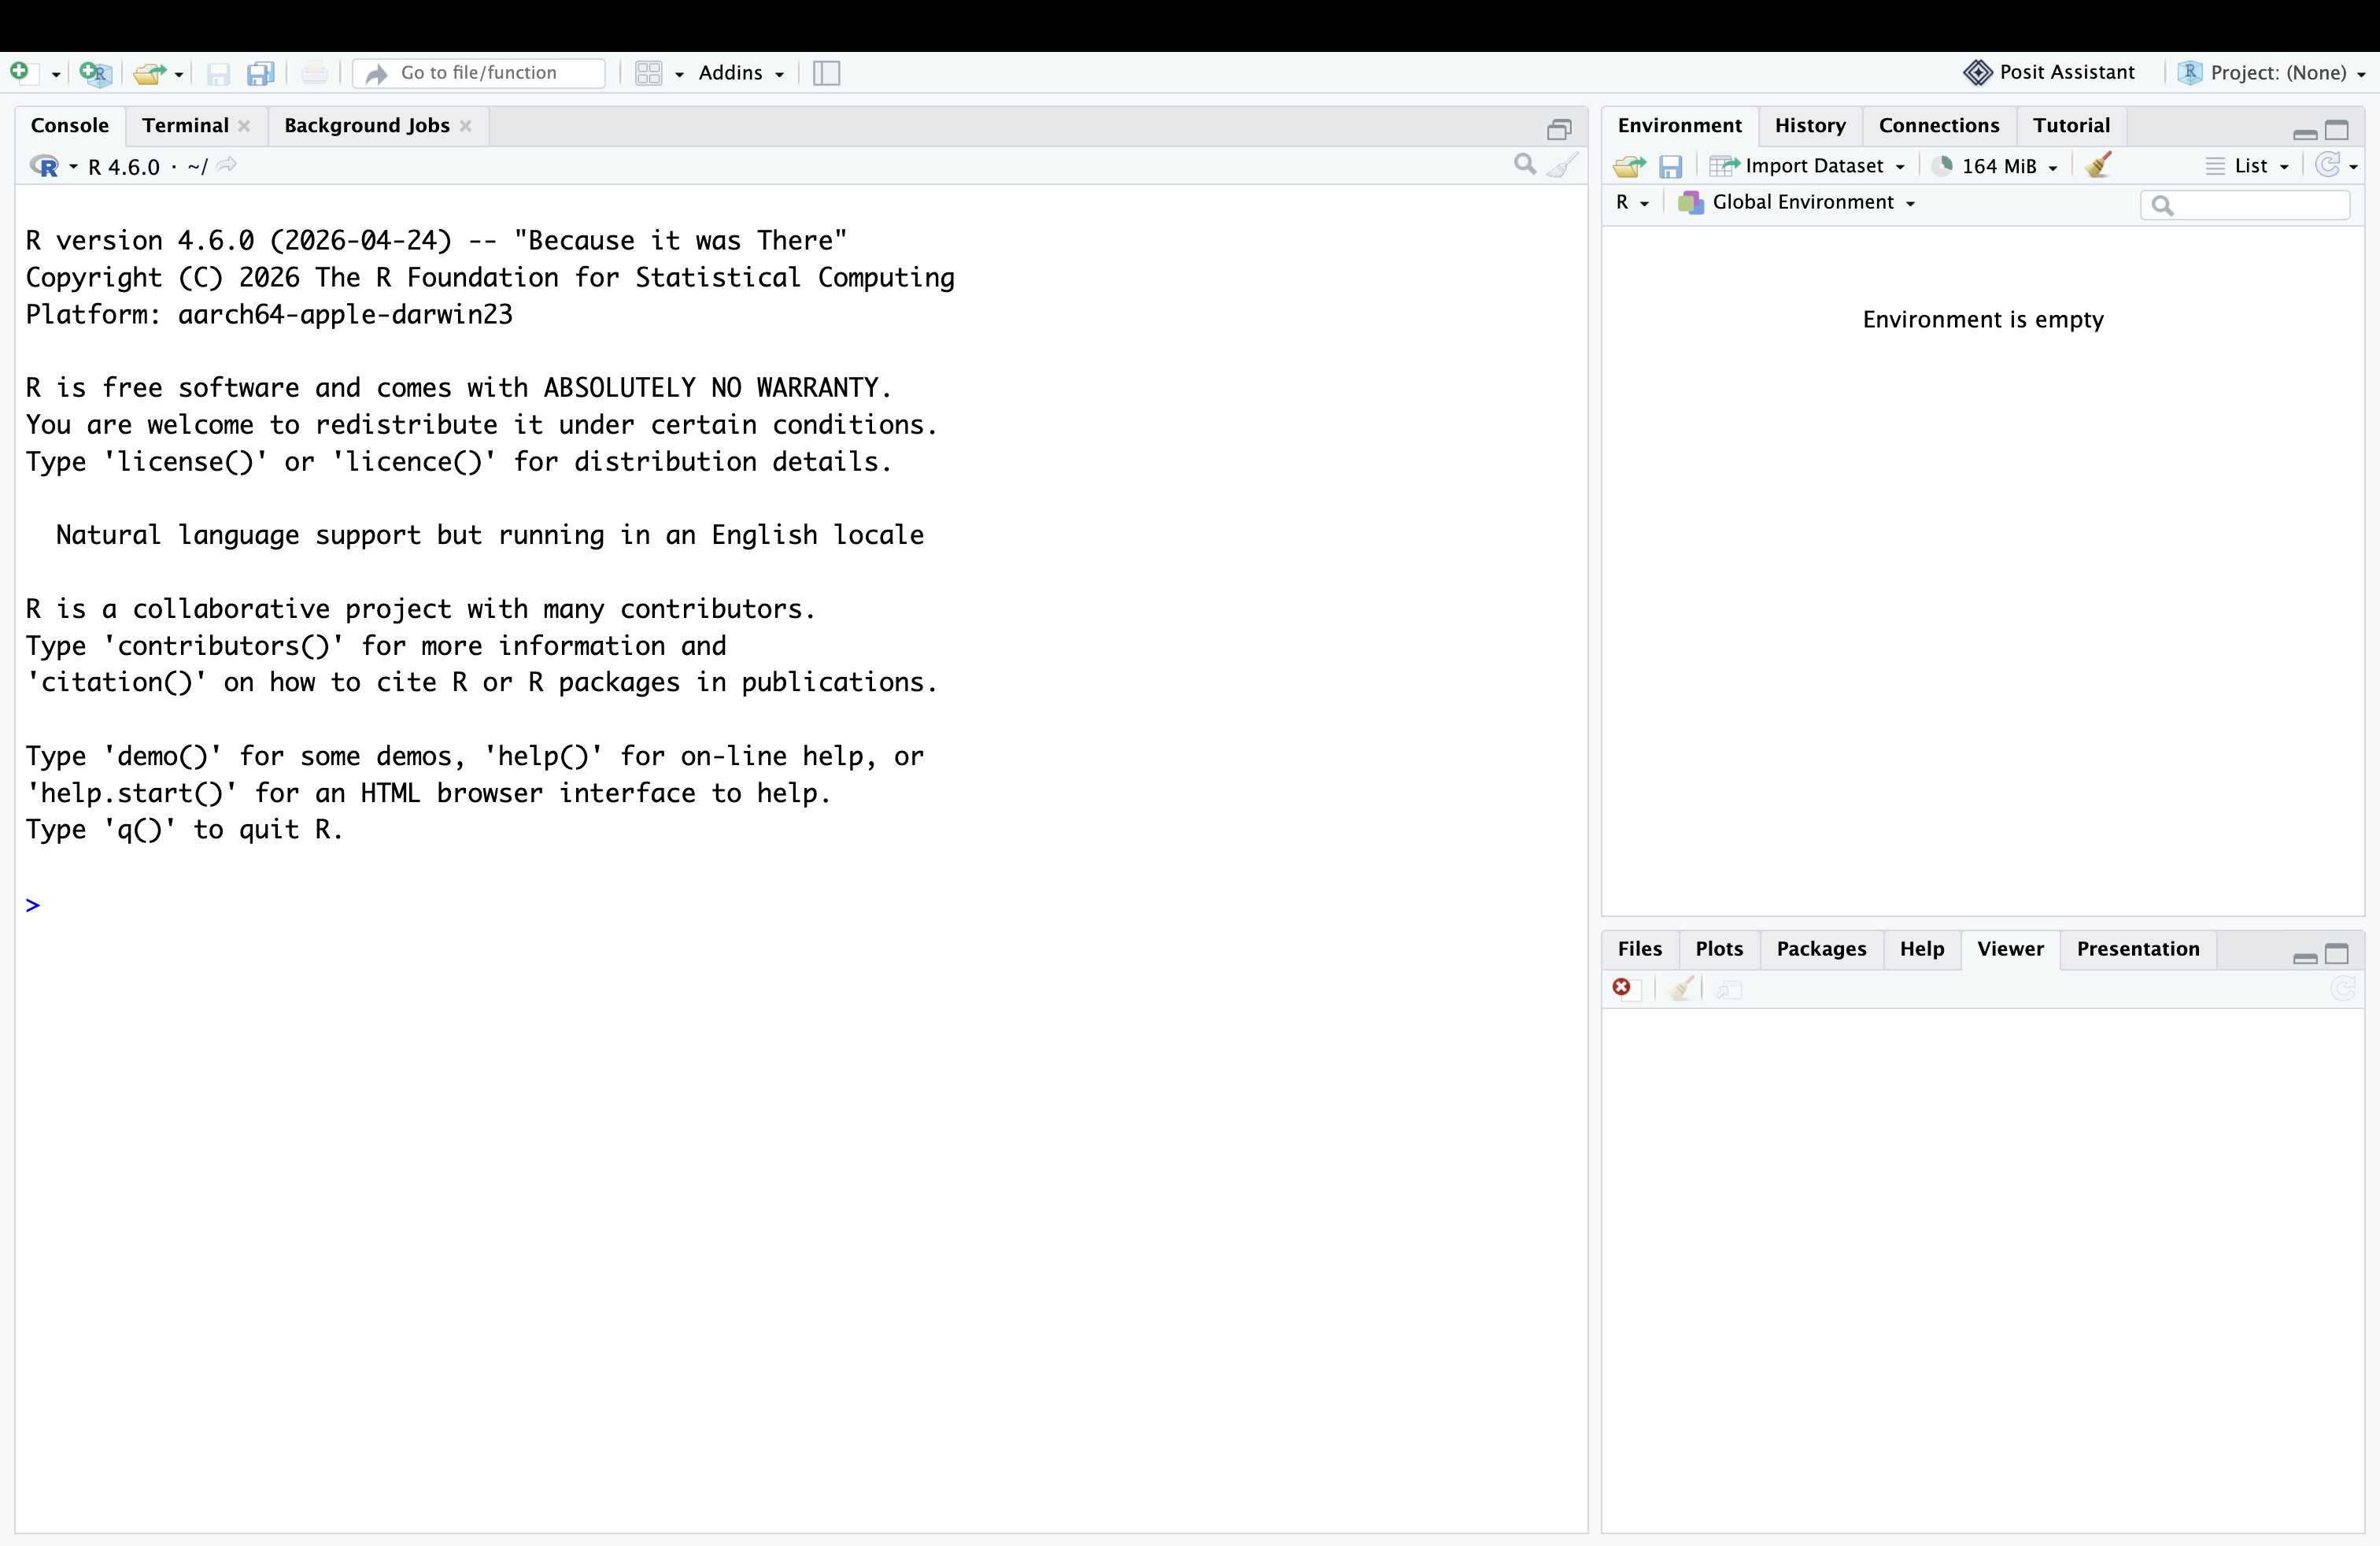
\includegraphics[width=1\textwidth,height=\textheight]{images/rstudio.png}

}

\caption{\label{fig-img-rstudio}RStudio interface}

\end{figure}%

You will learn more about how to use the features included in RStudio
throughout this course, but we recommend watching the
\href{https://posit.co/resources/videos/programming-part-1-writing-code-in-rstudio/}{RStudio
Essentials 1} series of videos from the Posit team (the company who
maintain RStudio). The video we link here lasts around 30 minutes and
gives a tour of the main parts of RStudio.

\subsection{Console vs.~scripts}\label{console-vs.-scripts}

When you first open up RStudio, you will not see an R script like above,
there will just be the console window taking up the whole left half. You
can write code in the console to test it out, but you cannot save that
code anywhere, and you would lose all your code if you closed down
RStudio.

For this chapter only, we will use the console window to show you some
simple R code, but from Chapter 2 - \hyperref[C2-repro-docs]{Creating
reproducible documents} - we will teach you to work in a type of R
script called an \textbf{R Markdown} document which ends with the file
name .Rmd.

You can open a new file in a number of ways, but the simplest is in the
top menu of RStudio, selecting
\textbf{\texttt{File\ \textgreater{}\textgreater{}\ New\ File\ \textgreater{}\textgreater{}\ R\ Markdown}}
and clicking OK. You will then be able to see the extra pane in the top
left like Figure Figure~\ref{fig-img-rstudio}.

\section{Writing code with functions and
arguments}\label{writing-code-with-functions-and-arguments}

R code is made up of \textbf{functions} and \textbf{arguments} that go
into the functions to create outputs. \textbf{Functions} in R execute
specific tasks and normally take one or more \textbf{arguments}. You can
think of these concepts like a spoken language as verbs (function) that
require a subject and an object (arguments). You could also think of
them as a kind of recipe. Some recipes (function) are quite simple and
have one or two ingredients (arguments), while other recipes are more
complicated with many ingredients (arguments).

You can spot functions as they end in round brackets (known as
parentheses, \texttt{()}), and the arguments go within the round
brackets. They tend to look a bit like this:

\begin{Shaded}
\begin{Highlighting}[]
\FunctionTok{function\_name}\NormalTok{(}\AttributeTok{argument1 =}\NormalTok{ value, }\AttributeTok{argument2 =}\NormalTok{ value)}
\end{Highlighting}
\end{Shaded}

That would be the layout of a function with two arguments and each
argument takes a value. Bare with us as these concepts might feel super
abstract until you start using them.

You will learn to use many functions throughout this book and you can
look up all the arguments that a function takes in the help
documentation by using the format \texttt{?function}. You will see some
arguments are required while others are optional. Optional arguments
will often use what is known as a default setting, value, or option
(normally specified in the help documentation) if you do not enter any
value.

As an example, let us look at the help documentation for the function
\texttt{rnorm()} - a function which randomly generates a set of numbers
from what is known as the \textbf{Normal Distribution}.

\subsection{Activity 1 - Finding help documentation for
functions}\label{activity-1---finding-help-documentation-for-functions}

Open up RStudio and in the console window (bottom left), type the
following code:

\begin{Shaded}
\begin{Highlighting}[]
\NormalTok{?rnorm}
\end{Highlighting}
\end{Shaded}

The help documentation for \texttt{rnorm()} should appear in the bottom
right help panel. In the \textbf{Usage} section of the help, we see that
\texttt{rnorm()} takes the following form:

\begin{Shaded}
\begin{Highlighting}[]
\FunctionTok{rnorm}\NormalTok{(n, }\AttributeTok{mean =} \DecValTok{0}\NormalTok{, }\AttributeTok{sd =} \DecValTok{1}\NormalTok{)}
\end{Highlighting}
\end{Shaded}

In the \textbf{Arguments} section of the help, there are explanations
for each of the arguments:

\begin{itemize}
\item
  \texttt{n} is the number of observations/numbers/data points we want
  to create,
\item
  \texttt{mean} is the \textbf{mean} of the observations/numbers/data
  points we will create.
\item
  and \texttt{sd} is the \textbf{standard deviation} of the
  observations/numbers/data points we will create.
\end{itemize}

In the \textbf{Details} section of the help, it notes that if no values
are entered for \texttt{mean} and \texttt{sd} it will use a default of 0
for the mean and 1 for the standard deviation. So, these are the values
the function will use for its arguments of \texttt{mean} and \texttt{sd}
if you do not state any. However, because there is no \textbf{default
value} for \texttt{n}, this means that you must state a value for the
arguments \texttt{n}, otherwise the code will not run.

This is all still a little abstract, so let us try an example. Still
using \texttt{rnorm()} let us set the required argument \texttt{n} to
ask R to produce 5 random numbers.

\subsection{Activity 2 - Running your first
function}\label{activity-2---running-your-first-function}

Type the following two lines of code into your console window. Press
enter/return on your keyboard at the end of each line to ``run'' that
line. So, type \texttt{set.seed(10072024)} and press enter/return and
then type \texttt{rnorm(n\ =\ 5)} and press enter/return. You will now
see these numbers in your console window:

\begin{verbatim}
[1] -0.6773381  2.9686894 -1.0461339 -1.4800300  0.4313315
\end{verbatim}

These numbers have a mean close to 0 (\emph{M} = 0.039) and a standard
deviation (\emph{SD}) close to 1 (\emph{SD} = 1.784) - they are not
exact because you only sampled a very small set and that sampling is
random.

\begin{tcolorbox}[enhanced jigsaw, breakable, colframe=quarto-callout-note-color-frame, arc=.35mm, opacitybacktitle=0.6, titlerule=0mm, colbacktitle=quarto-callout-note-color!10!white, colback=white, toprule=.15mm, bottomtitle=1mm, toptitle=1mm, title=\textcolor{quarto-callout-note-color}{\faInfo}\hspace{0.5em}{What does set.seed() do?}, bottomrule=.15mm, rightrule=.15mm, leftrule=.75mm, coltitle=black, left=2mm, opacityback=0]

You can get R to generate seemingly random numbers, but they are not
totally random. Computers generate random numbers through a predictable
process, but they pick a starting point based on something like the
clock time. If you run \texttt{rnorm(n\ =\ 5)} several times in the
console, you will see the five numbers are different each time. However,
when you run \texttt{set.seed(10072024)} first, you will get the same
five numbers every time, which is useful when you want a random but
reproducible set of numbers.

\end{tcolorbox}

Now, we can play with the function and change the additional arguments
to produce a different set of numbers. This time we will say we want 5
numbers again (\texttt{n\ =\ 5}) but we want our mean closer to 10
(\texttt{mean\ =\ 10}) and our standard deviation closer to 2
(\texttt{sd\ =\ 2}). We would do that as follows and you should see the
output numbers below.

\begin{Shaded}
\begin{Highlighting}[]
\FunctionTok{set.seed}\NormalTok{(}\DecValTok{10072024}\NormalTok{)}

\FunctionTok{rnorm}\NormalTok{(}\AttributeTok{n =} \DecValTok{5}\NormalTok{, }\AttributeTok{mean =} \DecValTok{10}\NormalTok{, }\AttributeTok{sd =} \DecValTok{2}\NormalTok{)}
\end{Highlighting}
\end{Shaded}

\begin{verbatim}
[1]  8.645324 15.937379  7.907732  7.039940 10.862663
\end{verbatim}

This time, we created 5 random numbers again, but this set has a mean
close to 10 (\emph{M} = 10.079) and a SD close to 2 (\emph{SD} = 3.569).
Hopefully, you are starting to get a sense of arguments within
functions, how you can change them, and how you can always remember to
use the help documentation to understand what arguments a function
requires.

Over time, you start to remember which arguments you need within
functions you commonly use, but even experienced R users have to
regularly check the documentation. Coding is not a memory test, so do
not worry if you find yourself needing to constantly look up the name of
arguments.

\begin{tcolorbox}[enhanced jigsaw, breakable, colframe=quarto-callout-important-color-frame, arc=.35mm, opacitybacktitle=0.6, titlerule=0mm, colbacktitle=quarto-callout-important-color!10!white, colback=white, toprule=.15mm, bottomtitle=1mm, toptitle=1mm, title=\textcolor{quarto-callout-important-color}{\faExclamation}\hspace{0.5em}{Error mode}, bottomrule=.15mm, rightrule=.15mm, leftrule=.75mm, coltitle=black, left=2mm, opacityback=0]

One thing that can be intimidating at first is making errors. They have
little red marks and produce sometimes vague messages to try and explain
what went wrong. You will make many errors as you learn and over time,
you do not stop making errors, but you get faster at working out what
went wrong and how you can fix it. So, we will introduce you to common
errors as we work through the book to help with problem solving.

Try and run the following code in the console:

\begin{Shaded}
\begin{Highlighting}[]
\FunctionTok{rnorm}\NormalTok{(}\AttributeTok{mean =} \DecValTok{10}\NormalTok{, }\AttributeTok{sd =} \DecValTok{2}\NormalTok{)}
\end{Highlighting}
\end{Shaded}

You should get an error saying something like
\texttt{Error\ in\ rnorm(mean\ =\ 10,\ sd\ =\ 2):\ argument\ "n"\ is\ missing,\ with\ no\ default}.
This error message is useful as it is telling us we forget to state the
\texttt{n} argument which has no default value, so the function has no
idea how many observations to give you. You would fix this error by
adding a value for \texttt{n} within the function.

\end{tcolorbox}

\subsection{Stating argument names}\label{stating-argument-names}

In the examples above, we have written out the argument names in our
code (for example, we wrote \texttt{n\ =\ 5}, \texttt{mean\ =\ 10},
\texttt{sd\ =\ 2}), however, this is not strictly necessary. The
following two lines of code would produce very similar outputs with the
same number of values and similar means and standard deviations.
Remember though: each time you run \texttt{rnorm()}, it will produce a
slightly different set of numbers unless you set a seed.

\begin{Shaded}
\begin{Highlighting}[]
\FunctionTok{rnorm}\NormalTok{(}\AttributeTok{n =} \DecValTok{6}\NormalTok{, }\AttributeTok{mean =} \DecValTok{3}\NormalTok{, }\AttributeTok{sd =} \DecValTok{1}\NormalTok{)}
\FunctionTok{rnorm}\NormalTok{(}\DecValTok{6}\NormalTok{, }\DecValTok{3}\NormalTok{, }\DecValTok{1}\NormalTok{)}
\end{Highlighting}
\end{Shaded}

The main thing is that both lines of code would still work - the code
knows what to do with the numbers. Both options work as the code is
following a set order of arguments: \texttt{n} then \texttt{mean} then
\texttt{sd}. If you do not write out the argument names, the code will
use the default order of arguments, which for \texttt{rnorm} will assume
that the first number you enter is \texttt{n}, the second number is
\texttt{mean}, and the third number is \texttt{sd}.

So, you can write the argument names or not, but it is important to know
the default order if you choose not to write the argument names.
Alternatively, if you write out the argument names, then you can write
the arguments in whatever order you like. The code below will still work
and produce six numbers with a mean close to 3 and a standard deviation
close to 1.

\begin{Shaded}
\begin{Highlighting}[]
\FunctionTok{rnorm}\NormalTok{(}\AttributeTok{sd =} \DecValTok{1}\NormalTok{, }
      \AttributeTok{n =} \DecValTok{6}\NormalTok{, }
      \AttributeTok{mean =} \DecValTok{3}\NormalTok{)}
\end{Highlighting}
\end{Shaded}

When you are first learning R, we recommend writing out the argument
names every time as it can help you remember and understand what each
part of the function is doing. However, as your skills progress you may
find it quicker to omit the argument names and you will also see
examples of code online that do not use argument names. In this course,
we will always write out the argument names the first time we use each
function, but afterwards, we may omit them.

\begin{tcolorbox}[enhanced jigsaw, breakable, colframe=quarto-callout-warning-color-frame, arc=.35mm, opacitybacktitle=0.6, titlerule=0mm, colbacktitle=quarto-callout-warning-color!10!white, colback=white, toprule=.15mm, bottomtitle=1mm, toptitle=1mm, title=\textcolor{quarto-callout-warning-color}{\faExclamationTriangle}\hspace{0.5em}{Warning}, bottomrule=.15mm, rightrule=.15mm, leftrule=.75mm, coltitle=black, left=2mm, opacityback=0]

If you do omit argument names, it is important to check the values you
use for arguments are the ones you intended to use. The sneakiest errors
are the ones that ``work'' in that they do not produce an error, but
they are doing something different to what you expect. For example, if
you wanted five numbers with a mean of 1 and \emph{SD} of 2,
\texttt{rnorm(5,\ 2,\ 1)} would work, but we accidentally entered the
mean and SD the wrong way around.

\end{tcolorbox}

\subsection{Tab auto-complete}\label{tab-auto-complete}

One very useful feature of RStudio is the tab auto-complete for
functions (see Figure Figure~\ref{fig-img-autocomplete}). If you write
the name of the function and then press the tab key on your keyboard,
RStudio will show you the arguments that function takes along with a
brief description. If you press enter on the argument name, it will fill
in the name for you, just like auto-complete on your phone.

You can also use the tab button when writing a function name to
auto-complete that function name or to find functions that start with
certain letters. This feature can be really helpful if you cannot quite
remember the name of a function or argument.

\begin{figure}

\centering{

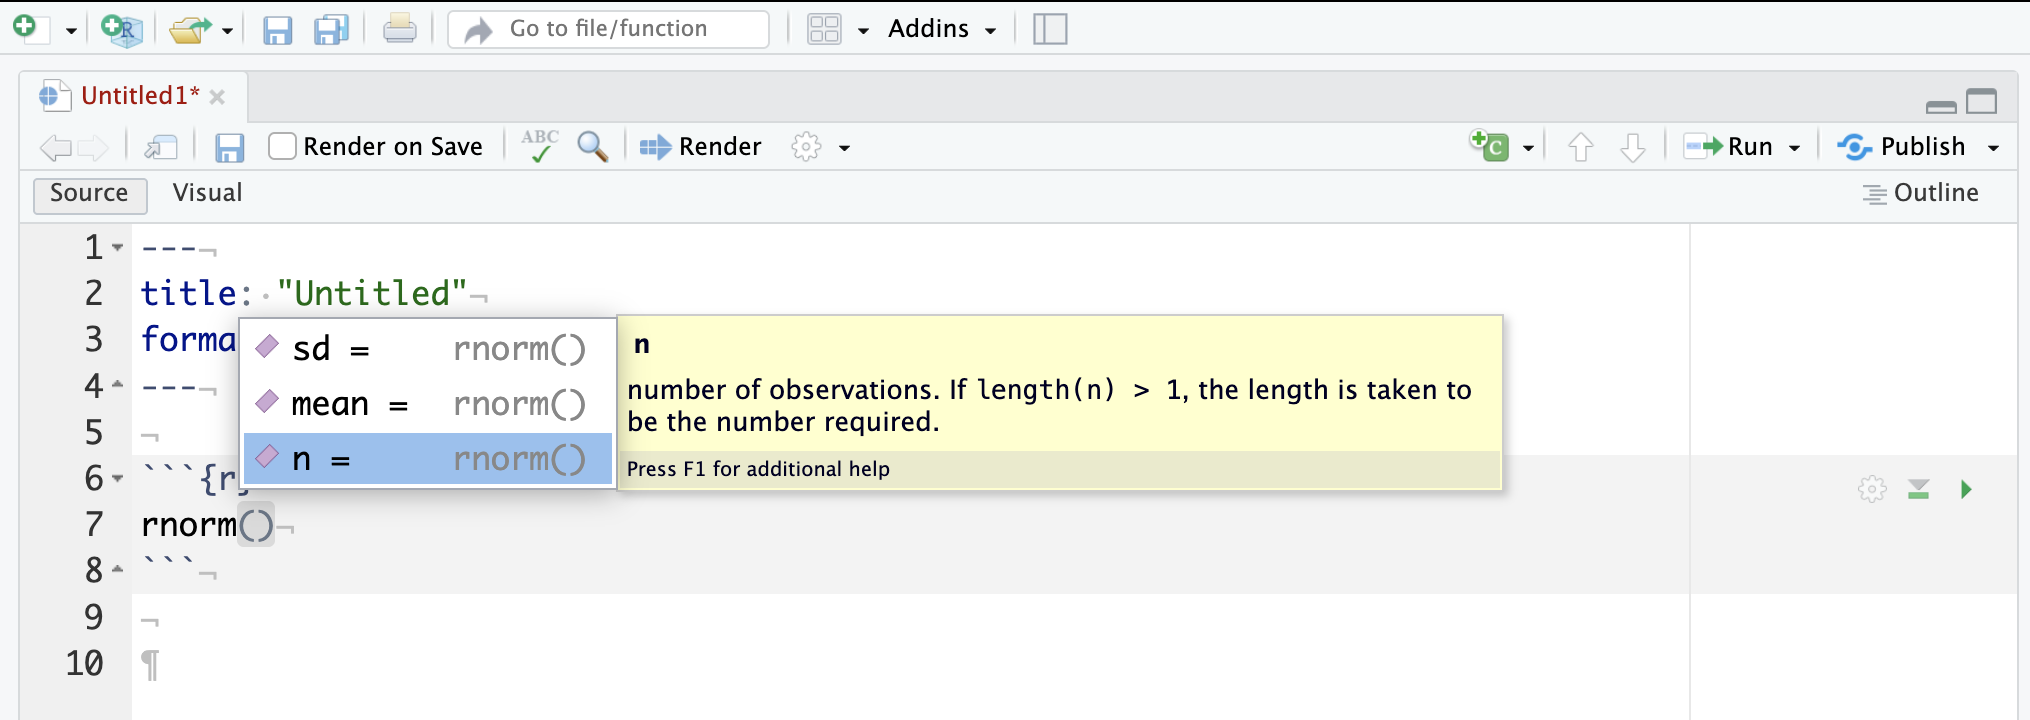
\includegraphics[width=1\textwidth,height=\textheight]{images/autocomplete.png}

}

\caption{\label{fig-img-autocomplete}Tab auto-complete}

\end{figure}%

\section{Base R and packages}\label{packages}

When you install R, you will have access to a range of functions
including options for data wrangling and statistical analysis. The
functions that are included in the default installation of R are
typically referred to as \textbf{Base R} and there is a useful cheat
sheet that shows many Base R functions about halfway down
\href{https://www.rstudio.com/resources/cheatsheets/}{this page under
Contributed Cheatsheets here}, along with a host of other cheatsheets
you might find useful.

However, the power of R is that it is extendable and open source. If a
function does not exist or does not work very well, anyone can create a
new \textbf{package} that contains data and/or code to allow you to
perform new tasks. You can think of \textbf{Base R} as the default apps
that come on your phone and other packages as additional apps; the ones
that you really want to use to make the phone your own, but you need to
download them separately.

\subsection{Activity 3 - Install the tidyverse to your own
computer}\label{install-tidy}

To use a package, you must first install it. The following code installs
the package \texttt{tidyverse}, a package we will use extensively
throughout this course and introduce in the next chapter.

\begin{tcolorbox}[enhanced jigsaw, breakable, colframe=quarto-callout-warning-color-frame, arc=.35mm, opacitybacktitle=0.6, titlerule=0mm, colbacktitle=quarto-callout-warning-color!10!white, colback=white, toprule=.15mm, bottomtitle=1mm, toptitle=1mm, title=\textcolor{quarto-callout-warning-color}{\faExclamationTriangle}\hspace{0.5em}{Warning}, bottomrule=.15mm, rightrule=.15mm, leftrule=.75mm, coltitle=black, left=2mm, opacityback=0]

\textbf{Please do not complete this activity if you are working on the
online R server or if you are using the computers in a University lab or
Boyd Orr Building}. You should only complete this activity on your own
device. The university computers and server already have a version of
all the packages we introduce you to, and installing a new version can
cause problems by having a conflict between one version on your user
profile and another version on the system profile.

\end{tcolorbox}

If you are working on your own computer, use the code below to install
the \textbf{tidyverse} and typing it into the console and pressing
enter/return. Remember: if you are using the online R server or using a
university computer, then skip this activity.

\begin{Shaded}
\begin{Highlighting}[]
\FunctionTok{install.packages}\NormalTok{(}\StringTok{"tidyverse"}\NormalTok{)}
\end{Highlighting}
\end{Shaded}

\begin{tcolorbox}[enhanced jigsaw, breakable, colframe=quarto-callout-important-color-frame, arc=.35mm, opacitybacktitle=0.6, titlerule=0mm, colbacktitle=quarto-callout-important-color!10!white, colback=white, toprule=.15mm, bottomtitle=1mm, toptitle=1mm, title=\textcolor{quarto-callout-important-color}{\faExclamation}\hspace{0.5em}{Important}, bottomrule=.15mm, rightrule=.15mm, leftrule=.75mm, coltitle=black, left=2mm, opacityback=0]

If you have a Windows computer and get an error message that says
something like ``WARNING: Rtools is required to build R packages'' you
may need to download and install an extra bit of software called
\href{https://cran.r-project.org/bin/windows/Rtools/}{Rtools}. This was
part of the R/RStudio installation instructions, so please see
\href{https://psyteachr.github.io/ug1-practical/installing-r.html}{Installing
R} for more detailed instructions.

\end{tcolorbox}

You only need to install a package once, but each time you start R /
RStudio, you must load the packages you want to use. This is like how
you need to install an app on your phone once, but you need to open it
every time you want to use it.

To load packages, we use the function \texttt{library()} which loads
packages into your working library. Typically, you would start any
analysis script by loading all of the packages you need, but we will
come back to that in the next chapter.

\subsection{Activity 4 - Load the
tidyverse}\label{activity-4---load-the-tidyverse}

Run the code below to load the tidyverse into your working library. You
must complete this activity regardless of whether you are using your own
computer or the university computers / online server.

\begin{Shaded}
\begin{Highlighting}[]
\FunctionTok{library}\NormalTok{(tidyverse)}
\end{Highlighting}
\end{Shaded}

Often when you load packages you get information in your console window.
Some packages will provide little messages to tell you what it has done
or warn you about something. Sometimes these messages can look like
errors and make you panic, but try and read over what it is saying
first. For example, you should have something that looks like Figure
Figure~\ref{fig-img-load-tidyverse} when you load \texttt{tidyverse}.
You might think you have done something wrong as it has little red
crosses, but it is just telling you that it has loaded a set of packages
and there are some \textbf{conflicts}.

\begin{figure}

\centering{

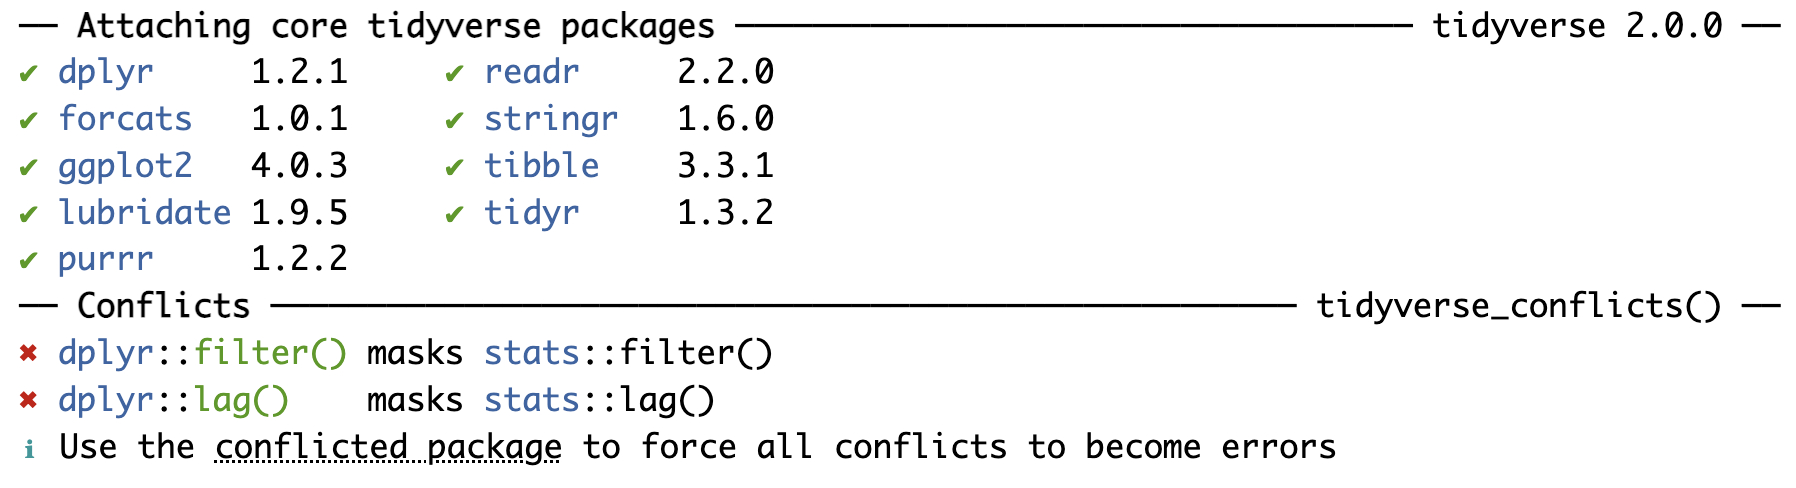
\includegraphics[width=1\textwidth,height=\textheight]{images/tidyverse-loading.png}

}

\caption{\label{fig-img-load-tidyverse}Example loading message from
tidyverse.}

\end{figure}%

Now that we have loaded the \texttt{tidyverse} package, we can use any
of the functions it contains but remember, you must run the
\texttt{library()} function every time you start R.

\subsection{Package updates}\label{package-updates}

In addition to updates to R and R Studio, the creators of packages also
update their code. This can be to add additional functions to a package,
or it can be to fix errors.

One thing to avoid is unintentionally updating an installed package.
When you run \texttt{install.packages()}, it will always install the
latest version of the package and it will overwrite any older versions
you may have installed. Often this is not a problem, but sometimes you
will find that the update means your code no longer works as the package
has changed substantially. It is possible to revert back to an older
version of a package but try to avoid updating a package
unintentionally.

\begin{tcolorbox}[enhanced jigsaw, breakable, colframe=quarto-callout-warning-color-frame, arc=.35mm, opacitybacktitle=0.6, titlerule=0mm, colbacktitle=quarto-callout-warning-color!10!white, colback=white, toprule=.15mm, bottomtitle=1mm, toptitle=1mm, title=\textcolor{quarto-callout-warning-color}{\faExclamationTriangle}\hspace{0.5em}{Warning}, bottomrule=.15mm, rightrule=.15mm, leftrule=.75mm, coltitle=black, left=2mm, opacityback=0]

To avoid accidentally overwriting a package with a later version, you
should \textbf{never} include \texttt{install.packages()} in your
analysis scripts in case you, or someone else runs the code by mistake.
Remember, the online server and university computers will already have
all of the packages you need for this course, so you only need to
install packages if you are using your own computer.

\end{tcolorbox}

\subsection{Package conflicts}\label{conflicts}

There are thousands of different R packages and each package has many
functions. Unfortunately, different people develop different packages
and sometimes they use the same name for different functions. For
example, the packages \texttt{dplyr} and \texttt{MASS} both have a
function called \texttt{select()}. \textbf{Do not run the below code},
but if you did you would see a warning telling you that there is a
conflict.

\begin{Shaded}
\begin{Highlighting}[]
\FunctionTok{library}\NormalTok{(dplyr)}
\end{Highlighting}
\end{Shaded}

\begin{verbatim}

Attaching package: 'dplyr'
\end{verbatim}

\begin{verbatim}
The following objects are masked from 'package:stats':

    filter, lag
\end{verbatim}

\begin{verbatim}
The following objects are masked from 'package:base':

    intersect, setdiff, setequal, union
\end{verbatim}

\begin{Shaded}
\begin{Highlighting}[]
\FunctionTok{library}\NormalTok{(MASS)}
\end{Highlighting}
\end{Shaded}

\begin{verbatim}

Attaching package: 'MASS'
\end{verbatim}

\begin{verbatim}
The following object is masked from 'package:dplyr':

    select
\end{verbatim}

You would see a warning that
\texttt{The\ following\ object\ is\ masked\ from\ \textquotesingle{}package:dplyr\textquotesingle{}:\ select}.

In this case, R is telling you that the function \texttt{select()} in
the \texttt{dplyr} package is being hidden (or `masked') by another
function with the same name from the \texttt{MASS} package. If you were
to try and use \texttt{select()}, R would use the function from the
package that was loaded most recently - in this case it would use the
function from \texttt{MASS}. This can be an issue because you think you
are using one function but really you are using another. They often work
differently and you get odd issues in your code that you do not expect.

There are various solutions but one simple one - if you already know of
the clash - is to specify which package you want to use for a particular
function by writing the code in the format \texttt{package::function},
meaning ``use the function from the package'', for example:

\begin{Shaded}
\begin{Highlighting}[]
\NormalTok{dplyr}\SpecialCharTok{::}\FunctionTok{select}\NormalTok{()}
\NormalTok{MASS}\SpecialCharTok{::}\FunctionTok{select}\NormalTok{()}
\end{Highlighting}
\end{Shaded}

Clashes are inevitable in your learning and when you see one, you will
probably not spot it at first but you will learn to resolve them
quickly.

\section{Objects}\label{objects}

So far, you have learnt about packages, and functions and arguments.
Earlier we said functions give us outputs and another name for outputs -
or at least specific types of outputs - are \textbf{objects}.

Objects are the output of functions but you can also create objects
without functions. Most of your coding will involve creating and
manipulating objects. Objects contain stuff, which could be numbers,
words, or the result of functions, operations, and analyses.

The first key thing to know about objects is how to create them and to
give them content. You assign content to an object using
\texttt{\textless{}-} - often called the ``left arrow'' or the
\textbf{assignment operator} which you can read as ``assigned to''. Note
that we do not use the \texttt{=} symbol as an assignment operator.
There is a large discussion on why objects are assigned content and not
equal to content but that is for another time. For now, just remember
that we assign (\texttt{\textless{}-}) content, be it words, numbers, or
function output, to objects.

\subsection{Activity 5 - Create some
objects}\label{activity-5---create-some-objects}

Type the following code into the console window and run each line. You
should see that \texttt{name}, \texttt{age}, \texttt{today},
\texttt{new\_year}, and \texttt{data} appear in the environment pane
like Figure Figure~\ref{fig-img-objects-enviro}.

\begin{Shaded}
\begin{Highlighting}[]
\NormalTok{name }\OtherTok{\textless{}{-}} \StringTok{"James"}
\NormalTok{age }\OtherTok{\textless{}{-}} \DecValTok{16} \SpecialCharTok{+} \DecValTok{14} 
\NormalTok{today }\OtherTok{\textless{}{-}} \FunctionTok{Sys.Date}\NormalTok{()}
\NormalTok{new\_year }\OtherTok{\textless{}{-}} \FunctionTok{as.Date}\NormalTok{(}\StringTok{"2025{-}01{-}01"}\NormalTok{)}
\NormalTok{data }\OtherTok{\textless{}{-}} \FunctionTok{rnorm}\NormalTok{(}\AttributeTok{n =} \DecValTok{10}\NormalTok{, }\AttributeTok{mean =} \DecValTok{15}\NormalTok{, }\AttributeTok{sd =} \DecValTok{3}\NormalTok{)}
\end{Highlighting}
\end{Shaded}

\begin{figure}

\centering{

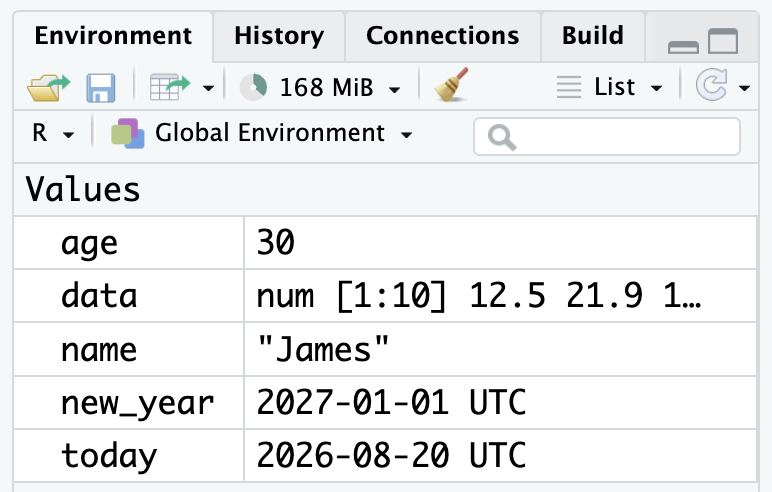
\includegraphics[width=1\textwidth,height=\textheight]{images/objects-enviro.png}

}

\caption{\label{fig-img-objects-enviro}Objects in the environment. Feel
free to change your numbers and check that they match the environment!}

\end{figure}%

Note that in these examples, \texttt{name},\texttt{age}, and
\texttt{new\_year} would always contain the values \texttt{James}, 30,
and the date of New Year's Day 2025, but \texttt{today} will draw the
date from the operating system on the day you are using the computer,
and \texttt{data} will be a randomly generated set of data - as we saw
earlier - so the values of these objects will not be static.

\begin{tcolorbox}[enhanced jigsaw, breakable, colframe=quarto-callout-tip-color-frame, arc=.35mm, opacitybacktitle=0.6, titlerule=0mm, colbacktitle=quarto-callout-tip-color!10!white, colback=white, toprule=.15mm, bottomtitle=1mm, toptitle=1mm, title=\textcolor{quarto-callout-tip-color}{\faLightbulb}\hspace{0.5em}{Try this}, bottomrule=.15mm, rightrule=.15mm, leftrule=.75mm, coltitle=black, left=2mm, opacityback=0]

Try changing the name to your name and the age to your age, and seeing
if they update in the environment window.

\end{tcolorbox}

Importantly, for what we will learn in future chapters, you can use
different objects in calculations and interact with each other. For
example:

\begin{Shaded}
\begin{Highlighting}[]
\NormalTok{age }\SpecialCharTok{+} \DecValTok{10}
\end{Highlighting}
\end{Shaded}

\begin{verbatim}
[1] 40
\end{verbatim}

\begin{Shaded}
\begin{Highlighting}[]
\NormalTok{new\_year }\SpecialCharTok{{-}}\NormalTok{ today}
\end{Highlighting}
\end{Shaded}

\begin{verbatim}
Time difference of -259 days
\end{verbatim}

\begin{Shaded}
\begin{Highlighting}[]
\FunctionTok{mean}\NormalTok{(data)}
\end{Highlighting}
\end{Shaded}

\begin{verbatim}
[1] 14.41643
\end{verbatim}

Finally, you can store the result of these operations on objects in a
new object as below:

\begin{Shaded}
\begin{Highlighting}[]
\NormalTok{decade }\OtherTok{\textless{}{-}}\NormalTok{ age }\SpecialCharTok{+} \DecValTok{10}
\end{Highlighting}
\end{Shaded}

Remember that you may find it helpful to read \texttt{\textless{}-} as
\texttt{contains} or \texttt{assigned\ to}, e.g., \texttt{name} contains
the text \texttt{James} or \texttt{James} is assigned to the object
\texttt{name}.

You will constantly be creating objects throughout this course and you
will learn more about them and how they behave as we go along. For now,
it is enough to understand that they are a way of saving values, that
these values can be numbers, text, or the result of operations, and that
you can use objects in further operations to create new objects.

\begin{tcolorbox}[enhanced jigsaw, breakable, colframe=quarto-callout-note-color-frame, arc=.35mm, opacitybacktitle=0.6, titlerule=0mm, colbacktitle=quarto-callout-note-color!10!white, colback=white, toprule=.15mm, bottomtitle=1mm, toptitle=1mm, title=\textcolor{quarto-callout-note-color}{\faInfo}\hspace{0.5em}{What should I call objects?}, bottomrule=.15mm, rightrule=.15mm, leftrule=.75mm, coltitle=black, left=2mm, opacityback=0]

In coding, we are trying to balance keeping objects names as short as
possible to be easy to type repeatedly, while being informative enough
that you know what they represent days, weeks, or months later when they
are not fresh in your memory.

For example, \texttt{dob} might save time now, but \texttt{birth\_date}
will be easier to understand in future.

\end{tcolorbox}

\subsection{Looking after the environment}\label{look-env}

Now that you are starting to learn about the other windows in RStudio
like the environment window, if you have been writing a lot of code, you
may find that the environment window (or workspace) becomes cluttered
with many objects. This can make it difficult to figure out which object
you need and you run the risk of using the wrong value or data frame. If
you are working on a new dataset, or if you have tried lots of different
code before getting the final version, it is good practice to remember
to clear the environment to avoid using the wrong object. You can do
this in several ways.

\begin{enumerate}
\def\labelenumi{\arabic{enumi}.}
\item
  To remove individual objects, you can type \texttt{rm(object\_name)}
  in the console. Try this now to remove one of the objects you created
  in the previous section. For example, you would remove the object
  \texttt{age} by writing \texttt{rm(age)}.
\item
  To clear all objects from the environment, run
  \texttt{rm(list\ =\ ls())} in the console.
\item
  To clear all objects from the environment, you can also click the
  broom icon in the environment pane like Figure
  Figure~\ref{fig-img-broom}.
\end{enumerate}

\begin{figure}

\centering{


\includegraphics[width=1\textwidth,height=\textheight]{images/broom.png}

}

\caption{\label{fig-img-broom}Clearing the workspace.}

\end{figure}%

\section{Global options}\label{global-options}

When you open RStudio, it will show you what you were last working on,
including your code and any objects you have created, assuming this is
not the first time you have used RStudio. This might sound helpful, but
it can cause more problems than it is worth because it means that you
risk accidentally using an old version of an object.

For example, you might have \texttt{Date} in the environment from the
last time you did some work and you start working on the wrong
\texttt{Date} without realising. In reality, we recommend changing the
settings so that each time you start RStudio, it opens a fresh new
environment.

You can do this by clicking on the top menu
\textbf{\texttt{Tools\ \textgreater{}\textgreater{}\ Global\ Options...}}
and then deselecting boxes so that your General box looks like Figure
Figure~\ref{fig-img-options} and applying the changes to save your
selections.

\begin{figure}

\centering{


\includegraphics[width=1\textwidth,height=\textheight]{images/global_options.png}

}

\caption{\label{fig-img-options}Global options - you want to make your
global options look similar, in terms of what is ticked, to the above.
The main thing is to make sure that you untick Restore RData into
workspace at startup, and set Save workspace to .RData on exit to Never.
Unticking the History options are optional but can help. The update
option is really just in case you want to.}

\end{figure}%

That should save a lot of hassle going forward. You will still encounter
issues of course, so we are going to end this chapter by outlining where
you can get help.

\section{Getting Help}\label{getting-help}

\subsection{Help and additional
resources}\label{help-and-additional-resources}

Learning to code really means trying stuff out, searching for help
online when it does not work, and finding examples of code to adapt to
your own needs.

If you are having difficulty with any of the content in this book, then
you can of course ask for help from the course team but learning to
problem solve effectively is a key skill that you will develop
throughout this course and beyond.

There are a wealth of \hyperref[additional-resources]{additional
resources} in the Appendix of this book, so it might be worth checking
them out, but here are four approaches we take to resolving an issue
when we hit a problem.

\begin{itemize}
\item
  Use the help documentation. If you are struggling to understand how a
  function works or what the arguments are, remember the
  \texttt{?function} command.
\item
  Think about when you last had to use this function or code
  successfully. Look back on what you did then and see what is the
  difference.
\item
  If you get an error message, copy and paste it into Google. It is very
  likely someone else has had the same problem.
\item
  Trying Googling your question in the style of the package name or
  function name and what you want to do. For example, \textbf{arrange
  data tidyverse} or maybe \textbf{sort data in R}.
\end{itemize}

If those approaches do not work, in addition to these course materials
and the other \href{https://psyteachr.github.io/}{PsyTeachR books} from
other courses we run, there are many excellent online resources for
learning data skills that can serve as quick guides:

\begin{itemize}
\item
  Individual package cheat sheets which you can find via the top menu:
  \textbf{\texttt{Help\ \textgreater{}\textgreater{}\ Cheat\ Sheets}}.
\item
  \href{http://www.cookbook-r.com/}{R Cookbook}.
\item
  \href{https://stackoverflow.com/}{StackOverflow}.
\item
  \href{https://r4ds.had.co.nz/}{R for Data Science}.
\end{itemize}

\subsection{Debugging tips}\label{debugging-tips}

Another top skill for resolving issues is what is known as debugging -
fixing your coding mistakes. A large part of coding is trying to figure
why your code does not work and this is true whether you are a novice or
an expert. As you progress through this course, try and keep a record of
mistakes you make and how you fixed them. We will highlight common
mistakes to look out for throughout the book but you will undoubtedly
make (and fix) new mistakes yourself.

You never stop making mistakes, you just get better at problem solving
and having a list of strategies that worked in the past. That is why we
include \textbf{error mode} as a set of activities to develop your
problem solving skills and normalise making errors.

As a short list of suggestions when you come across an error, keep in
mind:

\begin{itemize}
\item
  Have you loaded the correct packages for the functions you are trying
  to use? One common mistake is to write the code to load the package,
  e.g., \texttt{library(tidyverse)} but then forget to press
  enter/return to run it.
\item
  Have you made a typo? Coding has to be specific on spelling and
  \texttt{data} is not the same as \texttt{DATA}, and \texttt{t.test} is
  not the same as \texttt{t\_test}.
\item
  Is there a package conflict? Have you tried specifying the package and
  function with \texttt{package::function}?
\item
  Is it definitely an error? Not all red text in R / RStudio means an
  error. Sometimes it is just giving you a message with information.
\end{itemize}

\subsection{Activity 6 - Reset your R
session}\label{activity-6---reset-your-r-session}

Finally, if you find that your code is not working and you cannot figure
out why, it might be worth starting a new session. This will clear the
environment and detach all loaded packages. Think of it like restarting
your phone.

When you open up R and start writing code, loading packages, and
creating objects, you are typically doing so in a new \textbf{session}.
In addition to clearing your environment workspace, it can sometimes be
useful to start a new session. This will happen automatically each time
you start RStudio on your computer, although sessions can persist if you
use the online server.

This last activity shows a quick way to restart R from inside RStudio.
On the Top Menu, click
\textbf{\texttt{Session\ \textgreater{}\textgreater{}\ Restart\ R}} like
Figure Figure~\ref{fig-img-session}.

\begin{figure}

\centering{


\includegraphics[width=1\textwidth,height=\textheight]{images/new_session.png}

}

\caption{\label{fig-img-session}Restarting your R session from within
RStudio.}

\end{figure}%

Try not to worry about making mistakes. Accept that you will make them
and learn from them. We are always here to help if you are struggling,
so reach out to the course team, post on Teams, or attend a graduate
teaching assistant (GTA) session.

\section{Test yourself}\label{test-yourself}

Throughout the book, you will find additional questions and activities
like these to help you check your understanding. Some will have blanks
to fill in, some will be multiple choice, but the chapters include the
answers and explanations to check your understanding against. You are
always welcome to ask further questions to the course team though.

\subsection{Knowledge check}\label{knowledge-check}

\textbf{Question 1.} Why should you never include the code
\texttt{install.packages()} in your analysis scripts?

\begin{itemize}
\tightlist
\item
  \begin{enumerate}
  \def\labelenumi{(\Alph{enumi})}
  \tightlist
  \item
    You should use library() instead\\
  \end{enumerate}
\item
  \begin{enumerate}
  \def\labelenumi{(\Alph{enumi})}
  \setcounter{enumi}{1}
  \tightlist
  \item
    Packages are already part of Base R\\
  \end{enumerate}
\item
  \begin{enumerate}
  \def\labelenumi{(\Alph{enumi})}
  \setcounter{enumi}{2}
  \tightlist
  \item
    You (or someone else) may accidentally install a package update that
    stops your code working\\
  \end{enumerate}
\item
  \begin{enumerate}
  \def\labelenumi{(\Alph{enumi})}
  \setcounter{enumi}{3}
  \tightlist
  \item
    You already have the latest version of the package
  \end{enumerate}
\end{itemize}

\begin{tcolorbox}[enhanced jigsaw, breakable, colframe=quarto-callout-caution-color-frame, arc=.35mm, opacitybacktitle=0.6, titlerule=0mm, colbacktitle=quarto-callout-caution-color!10!white, colback=white, toprule=.15mm, bottomtitle=1mm, toptitle=1mm, title=\textcolor{quarto-callout-caution-color}{\faFire}\hspace{0.5em}{Explain this answer}, bottomrule=.15mm, rightrule=.15mm, leftrule=.75mm, coltitle=black, left=2mm, opacityback=0]

Remember, when you run \texttt{install.packages()} it will always
install the latest version of the package and it will overwrite any
older versions of the package you may have installed.

\end{tcolorbox}

\textbf{Question 2.} What will the following code produce?

\begin{Shaded}
\begin{Highlighting}[]
\FunctionTok{rnorm}\NormalTok{(}\DecValTok{6}\NormalTok{, }\DecValTok{50}\NormalTok{, }\DecValTok{10}\NormalTok{)}
\end{Highlighting}
\end{Shaded}

\begin{itemize}
\tightlist
\item
  \begin{enumerate}
  \def\labelenumi{(\Alph{enumi})}
  \tightlist
  \item
    A dataset with 10 numbers that has a mean of 6 and an SD of 50\\
  \end{enumerate}
\item
  \begin{enumerate}
  \def\labelenumi{(\Alph{enumi})}
  \setcounter{enumi}{1}
  \tightlist
  \item
    A dataset with 6 numbers that has a mean of 50 and an SD of 10\\
  \end{enumerate}
\item
  \begin{enumerate}
  \def\labelenumi{(\Alph{enumi})}
  \setcounter{enumi}{2}
  \tightlist
  \item
    A dataset with 50 numbers that has a mean of 10 and an SD of 6\\
  \end{enumerate}
\item
  \begin{enumerate}
  \def\labelenumi{(\Alph{enumi})}
  \setcounter{enumi}{3}
  \tightlist
  \item
    A dataset with 50 numbers that has a mean of 10 and an SD of 6
  \end{enumerate}
\end{itemize}

\begin{tcolorbox}[enhanced jigsaw, breakable, colframe=quarto-callout-caution-color-frame, arc=.35mm, opacitybacktitle=0.6, titlerule=0mm, colbacktitle=quarto-callout-caution-color!10!white, colback=white, toprule=.15mm, bottomtitle=1mm, toptitle=1mm, title=\textcolor{quarto-callout-caution-color}{\faFire}\hspace{0.5em}{Explain this answer}, bottomrule=.15mm, rightrule=.15mm, leftrule=.75mm, coltitle=black, left=2mm, opacityback=0]

The default form for \texttt{rnorm()} is \texttt{rnorm(n,\ mean,\ sd)}.
If you need help remembering what each argument of a function does, look
up the help documentation by running \texttt{?rnorm}.

\end{tcolorbox}

\textbf{Question 3.} If you have two packages that have functions with
the same name and you want to specify exactly which package to use, what
code would you use?

\begin{itemize}
\tightlist
\item
  \begin{enumerate}
  \def\labelenumi{(\Alph{enumi})}
  \tightlist
  \item
    package::function\\
  \end{enumerate}
\item
  \begin{enumerate}
  \def\labelenumi{(\Alph{enumi})}
  \setcounter{enumi}{1}
  \tightlist
  \item
    function::package\\
  \end{enumerate}
\item
  \begin{enumerate}
  \def\labelenumi{(\Alph{enumi})}
  \setcounter{enumi}{2}
  \tightlist
  \item
    library(package)\\
  \end{enumerate}
\item
  \begin{enumerate}
  \def\labelenumi{(\Alph{enumi})}
  \setcounter{enumi}{3}
  \tightlist
  \item
    install.packages(package)
  \end{enumerate}
\end{itemize}

\begin{tcolorbox}[enhanced jigsaw, breakable, colframe=quarto-callout-caution-color-frame, arc=.35mm, opacitybacktitle=0.6, titlerule=0mm, colbacktitle=quarto-callout-caution-color!10!white, colback=white, toprule=.15mm, bottomtitle=1mm, toptitle=1mm, title=\textcolor{quarto-callout-caution-color}{\faFire}\hspace{0.5em}{Explain this answer}, bottomrule=.15mm, rightrule=.15mm, leftrule=.75mm, coltitle=black, left=2mm, opacityback=0]

You should use the form \texttt{package::function}, for example
\texttt{dplyr::select}. Remember that when you first load your packages
R will warn you if any functions have the same name - remember to look
out for this!

\end{tcolorbox}

\textbf{Question 4.} Which of the following is most likely to be the
input to an argument?

\begin{itemize}
\tightlist
\item
  \begin{enumerate}
  \def\labelenumi{(\Alph{enumi})}
  \tightlist
  \item
    read\_csv()\\
  \end{enumerate}
\item
  \begin{enumerate}
  \def\labelenumi{(\Alph{enumi})}
  \setcounter{enumi}{1}
  \tightlist
  \item
    35\\
  \end{enumerate}
\item
  \begin{enumerate}
  \def\labelenumi{(\Alph{enumi})}
  \setcounter{enumi}{2}
  \tightlist
  \item
    \textless-
  \end{enumerate}
\end{itemize}

\begin{tcolorbox}[enhanced jigsaw, breakable, colframe=quarto-callout-caution-color-frame, arc=.35mm, opacitybacktitle=0.6, titlerule=0mm, colbacktitle=quarto-callout-caution-color!10!white, colback=white, toprule=.15mm, bottomtitle=1mm, toptitle=1mm, title=\textcolor{quarto-callout-caution-color}{\faFire}\hspace{0.5em}{Explain this answer}, bottomrule=.15mm, rightrule=.15mm, leftrule=.75mm, coltitle=black, left=2mm, opacityback=0]

read\_csv() looks like a function as it has the round brackets at the
end and the \textless- is the assignment symbol, so it is most likely
that 35 might be the input to an argument as it is just a value.

\end{tcolorbox}

\textbf{Question 5.} An easy way to spot functions is to look for

\begin{itemize}
\tightlist
\item
  \begin{enumerate}
  \def\labelenumi{(\Alph{enumi})}
  \tightlist
  \item
    round brackets\\
  \end{enumerate}
\item
  \begin{enumerate}
  \def\labelenumi{(\Alph{enumi})}
  \setcounter{enumi}{1}
  \tightlist
  \item
    computers\\
  \end{enumerate}
\item
  \begin{enumerate}
  \def\labelenumi{(\Alph{enumi})}
  \setcounter{enumi}{2}
  \tightlist
  \item
    numbers
  \end{enumerate}
\end{itemize}

\begin{tcolorbox}[enhanced jigsaw, breakable, colframe=quarto-callout-caution-color-frame, arc=.35mm, opacitybacktitle=0.6, titlerule=0mm, colbacktitle=quarto-callout-caution-color!10!white, colback=white, toprule=.15mm, bottomtitle=1mm, toptitle=1mm, title=\textcolor{quarto-callout-caution-color}{\faFire}\hspace{0.5em}{Explain this answer}, bottomrule=.15mm, rightrule=.15mm, leftrule=.75mm, coltitle=black, left=2mm, opacityback=0]

Remember that functions tend to have round brackets or parentheses at
the end of their name and the arguments and values go inside the
parentheses.

\end{tcolorbox}

\textbf{Question 6.} The job of \texttt{\textless{}-} is to send the
output from the function to a/an

\begin{itemize}
\tightlist
\item
  \begin{enumerate}
  \def\labelenumi{(\Alph{enumi})}
  \tightlist
  \item
    object\\
  \end{enumerate}
\item
  \begin{enumerate}
  \def\labelenumi{(\Alph{enumi})}
  \setcounter{enumi}{1}
  \tightlist
  \item
    assignment\\
  \end{enumerate}
\item
  \begin{enumerate}
  \def\labelenumi{(\Alph{enumi})}
  \setcounter{enumi}{2}
  \tightlist
  \item
    argument
  \end{enumerate}
\end{itemize}

\begin{tcolorbox}[enhanced jigsaw, breakable, colframe=quarto-callout-caution-color-frame, arc=.35mm, opacitybacktitle=0.6, titlerule=0mm, colbacktitle=quarto-callout-caution-color!10!white, colback=white, toprule=.15mm, bottomtitle=1mm, toptitle=1mm, title=\textcolor{quarto-callout-caution-color}{\faFire}\hspace{0.5em}{Explain this answer}, bottomrule=.15mm, rightrule=.15mm, leftrule=.75mm, coltitle=black, left=2mm, opacityback=0]

This is the assignment operator (\texttt{\textless{}-}) and we use it to
assign content such as the output of functions to an object.

\end{tcolorbox}

\subsection{Error mode}\label{error-mode-1}

The following questions are designed to introduce you to making and
fixing errors. Try and run the code, look at the error message, and see
if you can fix it before checking the answer. Consider keeping a note of
what kind of error messages you receive and how you fixed them, so you
have a bank of solutions when you tackle errors independently.

\textbf{Question 7.} Type the following code into the console and press
enter/return: \texttt{rnorm(n\ =\ 10,\ meen\ =\ 5,\ sd\ =\ 1)}. You
should get an error saying something like
\texttt{Error\ in\ rnorm(n\ =\ 10,\ meen\ =\ 5,\ sd\ =\ 1)\ :\ unused\ argument\ (meen\ =\ 5)}.
How can you fix it?

\begin{tcolorbox}[enhanced jigsaw, breakable, colframe=quarto-callout-caution-color-frame, arc=.35mm, opacitybacktitle=0.6, titlerule=0mm, colbacktitle=quarto-callout-caution-color!10!white, colback=white, toprule=.15mm, bottomtitle=1mm, toptitle=1mm, title=\textcolor{quarto-callout-caution-color}{\faFire}\hspace{0.5em}{Explain this answer}, bottomrule=.15mm, rightrule=.15mm, leftrule=.75mm, coltitle=black, left=2mm, opacityback=0]

We accidentally spelt one of the arguments incorrectly. If you look
closely, you will see that we typed \texttt{meen} spelt with two es
instead of one e when we should have typed \texttt{mean}.

\end{tcolorbox}

\textbf{Question 8.} To end on a sneaky one that we have not covered in
this chapter, type the following code into the console and press
enter/return: \texttt{rnorm(n\ =\ 10,\ mean\ =\ 5,\ sd\ =\ 1}. What
happened and how can you fix it? Before checking the explain this answer
box below, maybe try and Google what happens to see if you can describe
it and find a solution.

\begin{tcolorbox}[enhanced jigsaw, breakable, colframe=quarto-callout-caution-color-frame, arc=.35mm, opacitybacktitle=0.6, titlerule=0mm, colbacktitle=quarto-callout-caution-color!10!white, colback=white, toprule=.15mm, bottomtitle=1mm, toptitle=1mm, title=\textcolor{quarto-callout-caution-color}{\faFire}\hspace{0.5em}{Explain this answer}, bottomrule=.15mm, rightrule=.15mm, leftrule=.75mm, coltitle=black, left=2mm, opacityback=0]

We missed the final bracket, so we start the function name
\texttt{rnorm(}, enter our arguments, but there is no closing bracket.
You will see in the console like Figure
Figure~\ref{fig-img-unfinished-bracket}, there is a little \texttt{+}
symbol and you can enter new code, but there is no output.

\begin{figure}[H]

\centering{


\includegraphics[width=1\textwidth,height=\textheight]{images/unfinished-bracket.png}

}

\caption{\label{fig-img-unfinished-bracket}An R function without a
closing bracket in the console.}

\end{figure}%

This can be really frustrating as it looks like nothing is happening,
but when you did not add a closing bracket, R is just sitting there
waiting for you to add something else. To fix it, you can either type
\texttt{)} and press enter/return to finish the function and it should
work, or you can press the escape (esc) key to cancel the code and start
again.

\end{tcolorbox}

\section{Words from this Chapter}\label{words-from-this-chapter}

Below, you will find a list of words that we used in this chapter that
might be new to you in case you need to refer back to what they mean.
The links in this table take you to the entry for the words in the
\href{https://psyteachr.github.io/glossary/}{PsyTeachR Glossary}. Note
that numerous members of the team wrote entries in the Glossary and as
such the entries may use slightly different terminology from what we
used in the chapter.

\begin{longtable}[]{@{}
  >{\raggedright\arraybackslash}p{(\columnwidth - 2\tabcolsep) * \real{0.2512}}
  >{\raggedright\arraybackslash}p{(\columnwidth - 2\tabcolsep) * \real{0.7488}}@{}}
\toprule\noalign{}
\begin{minipage}[b]{\linewidth}\raggedright
term
\end{minipage} & \begin{minipage}[b]{\linewidth}\raggedright
definition
\end{minipage} \\
\midrule\noalign{}
\endhead
\bottomrule\noalign{}
\endlastfoot
\href{https://psyteachr.github.io/glossary/a\#argument}{argument} & A
variable that provides input to a function. \\
\href{https://psyteachr.github.io/glossary/a\#assignment-operator}{assignment-operator}
& The symbol \textless-, which functions like = and assigns the value on
the right to the object on the left \\
\href{https://psyteachr.github.io/glossary/b\#base-r}{base-r} & The set
of R functions that come with a basic installation of R, before you add
external packages. \\
\href{https://psyteachr.github.io/glossary/c\#conflict}{conflict} &
Having two packages loaded that have a function with the same name. \\
\href{https://psyteachr.github.io/glossary/c\#console}{console} & The
pane in RStudio where you can type in commands and view output
messages. \\
\href{https://psyteachr.github.io/glossary/d\#default-value}{default-value}
& A value that a function uses for an argument if it is skipped. \\
\href{https://psyteachr.github.io/glossary/e\#environment}{environment}
& A data structure that contains R objects such as variables and
functions \\
\href{https://psyteachr.github.io/glossary/f\#function}{function} & A
named section of code that can be reused. \\
\href{https://psyteachr.github.io/glossary/m\#mean}{mean} & A
descriptive statistic that measures the average value of a set of
numbers. \\
\href{https://psyteachr.github.io/glossary/n\#normal-distribution}{normal-distribution}
& A symmetric distribution of data where values near the centre are most
probable. \\
\href{https://psyteachr.github.io/glossary/o\#object}{object} & A word
that identifies and stores the value of some data for later use. \\
\href{https://psyteachr.github.io/glossary/p\#package}{package} & A
group of R functions. \\
\href{https://psyteachr.github.io/glossary/r\#r-markdown}{r-markdown} &
The R-specific version of markdown: a way to specify formatting, such as
headers, paragraphs, lists, bolding, and links, as well as code blocks
and inline code. \\
\href{https://psyteachr.github.io/glossary/r\#rstudio}{rstudio} & An
integrated development environment (IDE) that helps you process R
code. \\
\href{https://psyteachr.github.io/glossary/s\#script}{script} & A
plain-text file that contains commands in a coding language, such as
R. \\
\href{https://psyteachr.github.io/glossary/s\#session}{session} & When
you start R/RStudio and executive code to fill the workspace until you
close R/RStudio \\
\href{https://psyteachr.github.io/glossary/s\#standard-deviation}{standard-deviation}
& A descriptive statistic that measures how spread out data are relative
to the mean. \\
\href{https://psyteachr.github.io/glossary/t\#tidyverse}{tidyverse} & A
set of R packages that help you create and work with tidy data \\
\end{longtable}

\section{End of chapter}\label{end-of-chapter}

Well done on reaching the end of the first chapter! This was one of the
longest chapters in the book to introduce you to several foundational
concepts of coding in R and RStudio. The next chapter builds on these
skills to produce something a little more concrete by showing you how to
create reproducible documents.

\bookmarksetup{startatroot}

\chapter{Creating Reproducible Documents}\label{C02-repro-docs}

In this chapter, we introduce you to using code to create
\textbf{reproducible research}. Creating reproducible research means you
will write text and code that completely and transparently performs an
analysis from start to finish in a way that produces the same result for
different people using the same software on different computers. We will
cover things such as file structure and setting a working directory,
using \textbf{R Markdown} files, and writing code chunks.

As well as improving transparency with others researchers, reproducible
research benefits \textbf{you}. When you return to an analysis or task
after days, weeks, or months, you will thank past you for doing things
in a transparent, reproducible way, as you can easily pick up right
where you left off.

\textbf{Chapter Intended Learning Outcomes (ILOs)}

By the end of this chapter, you will be able to:

\begin{itemize}
\item
  Understand and set your working directory, either manually or through
  creating an R project.
\item
  Create a knit an R Markdown file to create a reproducible document.
\item
  Use inline code to combine text and code output in your reproducible
  documents.
\item
  Identify and fix common errors in knitting R Markdown files.
\end{itemize}

\section{File structure, working directories, and R
Projects}\label{02-projects}

In chapter 1, we never worked with files, so you did not have to worry
about where you put things on your computer. Before we can start working
with R Markdown files, we must explain what a \textbf{working directory}
is and how your computer knows where to find things.

Your working directory is the folder where your computer starts to look
for files. It would be able to access files from within that folder and
within sub-folders in your working directory, but it would not be able
to access folders outside your working directory.

In this course, we are going to prescribe a way of working to support an
organised file system, helping you to know where everything is and where
R will try to save things on your computer and where it will try to save
and load things. Once you become more comfortable working with files,
you can work in a different way that makes sense to you, but we
recommend following our instructions for at least RM1 as the first
course.

\subsection{Activity 1: Create a folder for all your
work}\label{intro-a1}

In your documents or OneDrive, create a new folder called
\texttt{ResearchMethods1\_2}. This will be your highest level folder
where you will save everything for Research Methods 1 and 2.

\begin{tcolorbox}[enhanced jigsaw, breakable, colframe=quarto-callout-tip-color-frame, arc=.35mm, opacitybacktitle=0.6, titlerule=0mm, colbacktitle=quarto-callout-tip-color!10!white, colback=white, toprule=.15mm, bottomtitle=1mm, toptitle=1mm, title=\textcolor{quarto-callout-tip-color}{\faLightbulb}\hspace{0.5em}{Top tip}, bottomrule=.15mm, rightrule=.15mm, leftrule=.75mm, coltitle=black, left=2mm, opacityback=0]

When you are a student at the University of Glasgow, you have access to
the full Microsoft suite of software. One of those is the cloud storage
system OneDrive. We heavily recommend using this to save all your work
in as it backs up your work online and you can access it from multiple
devices.

\end{tcolorbox}

Within that folder, create two new folders called \texttt{Assessments}
and \texttt{Quant\_Fundamentals}. In \texttt{Assessments}, you can save
all your assessments for RM1 and RM2 as you come to them. In
\texttt{Quant\_Fundamentals}, that is where you will save all your work
as you progress through this book.

Within \texttt{Quant\_Fundamentals}, create a new folder called
\texttt{Chapter\_02\_reproducible\_docs}. As you work through the book,
you will create a new chapter folder each time you start a new chapter
and the sub-folders will always be the same. Within
\texttt{Chapter\_02\_reproducible\_docs}, create two new folders called
\texttt{data} and \texttt{figures}. As a diagram, it should look like
Figure~\ref{fig-img-file-structure}.

\begin{figure}

\centering{


\includegraphics[width=1\textwidth,height=\textheight]{images/file-structure.png}

}

\caption{\label{fig-img-file-structure}Prescribed file structure for RM
1 and RM 2.}

\end{figure}%

\begin{tcolorbox}[enhanced jigsaw, breakable, colframe=quarto-callout-tip-color-frame, arc=.35mm, opacitybacktitle=0.6, titlerule=0mm, colbacktitle=quarto-callout-tip-color!10!white, colback=white, toprule=.15mm, bottomtitle=1mm, toptitle=1mm, title=\textcolor{quarto-callout-tip-color}{\faLightbulb}\hspace{0.5em}{How to name files and folders}, bottomrule=.15mm, rightrule=.15mm, leftrule=.75mm, coltitle=black, left=2mm, opacityback=0]

You might notice in the folder names we avoided using spaces by adding
things like underscores \_ or capitalising different words.
Historically, spaces in folder/file names could cause problems for code,
but now it's just slightly easier when file names and folder names do
not have spaces in them.

For naming files and folders, try and choose something sensible so you
know what it refers to. You are trying to balance being as short as
possible, while still being immediately identifiable. For example,
instead of fundamentals of quantitative analysis, we called it
\texttt{Quant\_Fundamentals}.

\end{tcolorbox}

\begin{tcolorbox}[enhanced jigsaw, breakable, colframe=quarto-callout-warning-color-frame, arc=.35mm, opacitybacktitle=0.6, titlerule=0mm, colbacktitle=quarto-callout-warning-color!10!white, colback=white, toprule=.15mm, bottomtitle=1mm, toptitle=1mm, title=\textcolor{quarto-callout-warning-color}{\faExclamationTriangle}\hspace{0.5em}{Warning}, bottomrule=.15mm, rightrule=.15mm, leftrule=.75mm, coltitle=black, left=2mm, opacityback=0]

When you create and name folders to use with R / RStudio, whatever you
do, do not call the folder ``R''. If you do this, sometimes R has an
identity crisis and will not save or load your files properly. It can
also really damage your setup and require you to reinstall everything as
R tends to save all the packages in a folder called R. If there is
another folder called R, then it gets confused and stops working
properly.

\end{tcolorbox}

\begin{tcolorbox}[enhanced jigsaw, breakable, colframe=quarto-callout-note-color-frame, arc=.35mm, opacitybacktitle=0.6, titlerule=0mm, colbacktitle=quarto-callout-note-color!10!white, colback=white, toprule=.15mm, bottomtitle=1mm, toptitle=1mm, title=\textcolor{quarto-callout-note-color}{\faInfo}\hspace{0.5em}{File management when using the online server}, bottomrule=.15mm, rightrule=.15mm, leftrule=.75mm, coltitle=black, left=2mm, opacityback=0]

If we support you to use the online University of Glasgow \textbf{R
Server}, working with files is a little different. If you downloaded R /
RStudio to your own computer or you are using one of the library/lab
computers, please ignore this section.

The main disadvantage to using the R server is that you will need create
folders on the server and then upload and download any files you are
working on to and from the server. Please be aware that \textbf{there is
no link between your computer and the R server}. If you change files on
the server, they will not appear on your computer until you download
them from the server, and you need to be very careful when you submit
your assessment files that you are submitting the right file. This is
the main reason we recommend installing R / RStudio on your computer
wherever possible.

Going forward throughout this book, if you are using the server, you
will need to follow an extra step where you also upload them to the
sever. As an example:

\begin{enumerate}
\def\labelenumi{\arabic{enumi}.}
\item
  Log on to the \textbf{R server} using the link we provided to you.
\item
  In the file pane, click \texttt{New\ folder} and create the same
  structure we demonstrated above.
\item
  Download \texttt{ahi-cesd.csv} and \texttt{participant-info.csv} into
  the \texttt{data} folder you created for chapter 2. To download a file
  from this book, right click the link and select ``save link as''. Make
  sure that both files are saved as ``.csv''. Do not open them on your
  machine as often other software like Excel can change setting and ruin
  the files.
\item
  Now that the files are stored on your computer, go to RStudio on the
  server and click \texttt{Upload} then \texttt{Browse} and choose the
  folder for the chapter you are working on.
\item
  Click \texttt{Choose\ file} and go and find the data you want to
  upload.
\end{enumerate}

\end{tcolorbox}

\subsection{Manually setting the working directory}\label{intro-a2}

Now that you have a folder structure that will keep everything nice and
organised, we will demonstrate how you can manually \textbf{set the
working directory}. If you open RStudio, you can check where the current
working directory is by typing the function \texttt{getwd()} into the
console and pressing enter/return. That will show you the current file
path R is using to navigate files. If you look at the Files window in
the bottom right, this will also show you the files and folders
available from your working directory.

If you click on the top menu
\textbf{\texttt{Session\ \textgreater{}\textgreater{}\ Set\ Working\ Directory\ \textgreater{}\textgreater{}\ Choose\ Directory...}},
(Figure~\ref{fig-img-working-dir}) you can navigate through your
documents or OneDrive until you can select
\texttt{Chapter\_02\_reproducible\_docs}. Click open and that will set
the folder as your working directory. You can double check this worked
by running \texttt{getwd()} again in the console.

\begin{figure}

\centering{


\includegraphics[width=1\textwidth,height=\textheight]{images/working-dir.png}

}

\caption{\label{fig-img-working-dir}Manually setting the working
directory.}

\end{figure}%

\subsection{Activity 2 - Creating an R
Project}\label{activity-2---creating-an-r-project}

Knowing how to check and manually set your working directory is useful,
but there is a more efficient way of setting your working directory
alongside organised file management. You are going to create something
called an \textbf{R Project}.

To create a new project for the work you will do in this chapter
(Figure~\ref{fig-new-proj}):

\begin{enumerate}
\def\labelenumi{\arabic{enumi}.}
\item
  Click on the top menu and navigate to
  \texttt{File\ \textgreater{}\textgreater{}\ New\ Project...}.
\item
  You have the option to select from New Directory, Existing Directory,
  or Version Control. You already created a folder for
  \texttt{Chapter\_02\_reproducible\_docs}, so select Existing
  Directory.
\item
  Click Browse\ldots{} next to Project working directory to select the
  folder you want to create the project in.
\item
  When you have navigated to \texttt{Chapter\_02\_reproducible\_docs}
  for this chapter, click Open and then Create Project.
\end{enumerate}

\begin{figure}

\begin{minipage}{0.50\linewidth}

\includegraphics{images/project-pageone.png}\end{minipage}%
%
\begin{minipage}{0.50\linewidth}

\includegraphics{images/project-pagetwo.png}\end{minipage}%

\caption{\label{fig-new-proj}Starting a new project.}

\end{figure}%

RStudio will restart itself and open with this new project directory as
the working directory. You should see something like
Figure~\ref{fig-img-project-screen}.

\begin{figure}

\centering{


\includegraphics[width=1\textwidth,height=\textheight]{images/new_project.png}

}

\caption{\label{fig-img-project-screen}RStudio screen in a new project
in your chapter 2 folder.}

\end{figure}%

In the files tab in the bottom right window, you will see all the
contents in your project directory. You can see your two sub-folders for
data and figures and a file called
\texttt{Chapter\_02\_reproducible\_docs.Rproj}. This is a file that
contains all of the project information. When you come back to this
project after closing down RStudio, if you double click on the .Rproj
file, it will open up your project and have your working directory all
set up and ready to go.

\begin{tcolorbox}[enhanced jigsaw, breakable, colframe=quarto-callout-warning-color-frame, arc=.35mm, opacitybacktitle=0.6, titlerule=0mm, colbacktitle=quarto-callout-warning-color!10!white, colback=white, toprule=.15mm, bottomtitle=1mm, toptitle=1mm, title=\textcolor{quarto-callout-warning-color}{\faExclamationTriangle}\hspace{0.5em}{Warning}, bottomrule=.15mm, rightrule=.15mm, leftrule=.75mm, coltitle=black, left=2mm, opacityback=0]

In each chapter, we will repeat these instructions at the start to
prescribe this file structure, but when you create your own folders and
projects, do not ever save a new project \textbf{inside} another
project. This can cause some hard to resolve problems. For example, it
would be fine to create a new project within the
\texttt{Quant\_Fundamentals} folder as we will do for each new chapter,
but should never create a new project within the
\texttt{Chapter\_02\_reproducible\_docs} folder.

\end{tcolorbox}

\section{Creating and navigating R Markdown
documents}\label{creating-and-navigating-r-markdown-documents}

Now you know how to navigate files and folders on your computer, we can
start working with R Markdown files.

Throughout this data skills book and related assignments, you will use a
file format called R Markdown (abbreviated as .Rmd) which is a great way
to create dynamic documents combining regular text and embedded code
chunks.

R Markdown documents are self-contained and fully reproducible, meaning
if you have the necessary data, you should be able to run someone else's
analyses. This is an important part of your open science training as one
of the reasons we teach data skills this way is that it enables us to
share open and reproducible information.

Using these worksheets enables you to keep a record of all the code you
write as you progress through this book (as well as any notes to help
yourself), for data skills assessments we can give you a task to add
required code, and in your research reports you can independently
process, visualise, and analyse your data all from one file.

For more information about R Markdown, feel free to have a look at their
main webpage \url{http://rmarkdown.rstudio.com}, but for now the key
advantage to know about is that it allows you to write code into a
document, along with regular text, and then \textbf{knit} it to create
your document as either a webpage (\textbf{html}), a PDF, or Word
document (.docx).

\subsection{Activity 3: Open, save, and knit a new R Markdown
document}\label{intro-a3}

Open a new R Markdown document by clicking the `new item' icon and then
click `R Markdown' like Figure~\ref{fig-img-new-markdown}.

\begin{figure}

\begin{minipage}{0.50\linewidth}

\includegraphics{images/Create_Rmd_menu.png}\end{minipage}%
%
\begin{minipage}{0.50\linewidth}

\includegraphics{images/Create_Rmd_options.png}\end{minipage}%

\caption{\label{fig-img-new-markdown}Creating a new R Markdown document
from the menu (left) and setting title, author, date, and output
(right).}

\end{figure}%

After selecting R Markdown, there are different format options you can
explore in time, but Select Document and there are four boxes to
complete:

\begin{itemize}
\item
  Title: This is the title for the document which will appear at the top
  of the page. For this chapter, enter
  \texttt{02\ Creating\ Reproducible\ Documents}.
\item
  Author: This is where you can add your name or names for multiple
  people. For this chapter, enter your GUID as this will be good
  practice for the data skills assignments.
\item
  Date: By default, it adds today's date, so it will update every time
  you knit the document. Leave the default so you know when you
  completed the chapter, but if you untick, you can manually enter a
  static date.
\item
  Default Output Format: You have the option to select from html, PDF,
  and Word. We will demonstrate how to change output format in a later
  chapter, so keep html for now as it's the most flexible format.
\end{itemize}

Once you click \textbf{OK}, this will open a new R Markdown document.

Save this R Markdown document by clicking
\textbf{\texttt{File\ \textgreater{}\textgreater{}\ Save\ as}} from the
top menu, and name this file ``\texttt{02\_reproducible\_docs}''. Note
the document title and file name are separate, so you still have to name
the file when you save it.

If you have set the working directory correctly, you should now see this
file appear in your Files window in the bottom right hand corner like
Figure~\ref{fig-img-file-dir}, alongside your .Rproj file and two
folders.

\begin{figure}

\centering{


\includegraphics[width=1\textwidth,height=\textheight]{images/Files_newRmd.png}

}

\caption{\label{fig-img-file-dir}New .Rmd file in your working
directory.}

\end{figure}%

Now you have the default version of the R Markdown file, you have a
bunch of text and code to show its capabilities
(Figure~\ref{fig-img-markdown-default}).

\begin{figure}

\centering{


\includegraphics[width=1\textwidth,height=\textheight]{images/Default_Rmd.png}

}

\caption{\label{fig-img-markdown-default}Default text and code in a new
R Markdown document.}

\end{figure}%

We will now demonstrate what it looks like to \textbf{knit} a document.
This means that we are going to compile (i.e., turn) our code into a
document that is more presentable. This way, you can check it knits and
there are no errors. So, as we add changes in the following activities,
you can identify if and when any errors appear and fix them quicker.

At the top of your R Markdown window, you should see a Knit button next
to a little ball of yarn (Figure~\ref{fig-img-knit-document}). If you
click that, the document will knit and produce a html file.

\begin{figure}

\centering{


\includegraphics[width=1\textwidth,height=\textheight]{images/knit_document.png}

}

\caption{\label{fig-img-knit-document}Clicking the knit button on a .Rmd
document.}

\end{figure}%

You will see a small version of the knitted document appear in the
Viewer tab in the bottom right of your screen. You will also see it has
created a new file in your working directory. It will have the same name
as your R Markdown file, but with .html as the file ending. You can view
the knitted document by clicking the ``Show in new window'' button or
opening the file from your folder
(Figure~\ref{fig-img-knitted-default}). This should open the document in
your default internet browser as websites are created in html.

\begin{figure}

\begin{minipage}{0.50\linewidth}

\includegraphics{images/Knitted_default_files.png}\end{minipage}%
%
\begin{minipage}{0.50\linewidth}

\includegraphics{images/Knitted_default_browser.png}\end{minipage}%

\caption{\label{fig-img-knitted-default}On the left, you can see a small
version of the knitted document in the Viewer tab. On the right, you can
see the full version open in your internet browser.}

\end{figure}%

Now everything is working and knitting, we can start editing the R
Markdown file to add new content.

\subsection{Activity 4: Create a new code chunk}\label{intro-a4}

Let's start using your new R Markdown document to combine code and text.
Follow these steps:

\begin{enumerate}
\def\labelenumi{\arabic{enumi}.}
\tightlist
\item
  Delete \textbf{everything} below line 10.
\end{enumerate}

\begin{tcolorbox}[enhanced jigsaw, breakable, colframe=quarto-callout-note-color-frame, arc=.35mm, opacitybacktitle=0.6, titlerule=0mm, colbacktitle=quarto-callout-note-color!10!white, colback=white, toprule=.15mm, bottomtitle=1mm, toptitle=1mm, title=\textcolor{quarto-callout-note-color}{\faInfo}\hspace{0.5em}{What does the \{r setup\} chunk do?}, bottomrule=.15mm, rightrule=.15mm, leftrule=.75mm, coltitle=black, left=2mm, opacityback=0]

At the moment, you do not need to worry about the code chunk between
lines 8 and 10. We are slowly introducing you to different features in R
Markdown as it's easier to understand by doing, rather than giving you a
list of explanations.

If you are really curious though, this setting forces R Markdown to show
both the code and output for all code chunks. When we add code shortly,
if you change it to \texttt{echo\ =\ FALSE}, it will only show the
output and not the code.

\end{tcolorbox}

\begin{enumerate}
\def\labelenumi{\arabic{enumi}.}
\setcounter{enumi}{1}
\item
  On line 12, type ``\#\# About me''.
\item
  With your cursor on line 14, insert a blank code chunk by clicking on
  the top menu
  \textbf{\texttt{Code\ \textgreater{}\textgreater{}\ Insert\ Chunk}} or
  using the shortcut at the top of the R Markdown window that looks like
  a small green c and select R.
\end{enumerate}

Your document should now look something like
Figure~\ref{fig-img-new-chunk}.

\begin{figure}

\centering{


\includegraphics[width=1\textwidth,height=\textheight]{images/Rmd_blank_insert_chunk.png}

}

\caption{\label{fig-img-new-chunk}Creating a new R chunk in your blank R
Markdown document}

\end{figure}%

What you have created is called a \textbf{code chunk}. R Markdown
assumes anything written outside of a code chunk is just normal text,
just like you would have in a text editor like Word. It assumes anything
written inside the code chunk is R code. This makes it easy to combine
both text and code in one document.

\begin{tcolorbox}[enhanced jigsaw, breakable, colframe=quarto-callout-important-color-frame, arc=.35mm, opacitybacktitle=0.6, titlerule=0mm, colbacktitle=quarto-callout-important-color!10!white, colback=white, toprule=.15mm, bottomtitle=1mm, toptitle=1mm, title=\textcolor{quarto-callout-important-color}{\faExclamation}\hspace{0.5em}{Error mode}, bottomrule=.15mm, rightrule=.15mm, leftrule=.75mm, coltitle=black, left=2mm, opacityback=0]

When you create a new code chunk, you should notice that the grey box
starts and ends with three back ticks
(\texttt{\textasciigrave{}\textasciigrave{}\textasciigrave{}}), followed
by the \{r\}, and then it ends with three back ticks again. This is the
structure that creates a code chunk. You could actually just type this
structure instead of using the \texttt{Insert} approach but we are
introducing you to some shortcuts

One common mistake is to accidentally delete one or more of these back
ticks. A useful thing to notice is that code chunks tend to have a
different color background - in the default appearance of RStudio a code
chunk is grey and the normal text is white. You can use this to look for
mistakes. If the colour of certain parts of your Markdown does not look
right, check that you have not deleted the backticks.

Remember it is backticks (i.e.~this `) and not single quotes (i.e.~not
this ').

\end{tcolorbox}

\begin{tcolorbox}[enhanced jigsaw, breakable, colframe=quarto-callout-note-color-frame, arc=.35mm, opacitybacktitle=0.6, titlerule=0mm, colbacktitle=quarto-callout-note-color!10!white, colback=white, toprule=.15mm, bottomtitle=1mm, toptitle=1mm, title=\textcolor{quarto-callout-note-color}{\faInfo}\hspace{0.5em}{Markdown language}, bottomrule=.15mm, rightrule=.15mm, leftrule=.75mm, coltitle=black, left=2mm, opacityback=0]

When you typed ``\#\# About me'', you might notice the two hashes. You
will see the effect of this shortly, but this is using \textbf{Markdown}
language to add document formatting. Markdown is a type of formatting
language, so instead of using buttons to add features like you would in
Word, you add symbols which will produce different features when you
knit the document.

The hashes create headers. One (\#) creates a first level header (larger
text), two (\#\#) creates a second level header, and so on. Make sure
there is a space between the text and hash or it will not knit properly.

As we progress through the book, we will slowly introduce you to
different Markdown features, but you can see the
\href{https://rmarkdown.rstudio.com/lesson-8.html}{RStudio Markdown
Basics page} if you are interested.

\end{tcolorbox}

\subsection{Activity 5: Write some code}\label{intro-a5}

Now we are going to use the code examples you read about in Chapter 1 -
\hyperref[C01-programming-basics]{Introduction to programming with R/R
Studio} - to add some code to our R Markdown document.

In your code chunk, write the code below but replace the values of
name/age/birthday with your own details). Remember that the four lines
of code should all be inside the code chunk.

\textbf{Note:} Text and dates need to be contained in quotation marks,
e.g., ``my name''. Numerical values are written without quotation marks,
e.g., 45.

\begin{Shaded}
\begin{Highlighting}[]
\NormalTok{name }\OtherTok{\textless{}{-}} \StringTok{"James"} 
\NormalTok{age }\OtherTok{\textless{}{-}} \DecValTok{30}
\NormalTok{today }\OtherTok{\textless{}{-}} \FunctionTok{Sys.Date}\NormalTok{()}
\NormalTok{next\_birthday }\OtherTok{\textless{}{-}} \FunctionTok{as.Date}\NormalTok{(}\StringTok{"2025{-}02{-}18"}\NormalTok{) }\CommentTok{\# Year, month, day format}
\end{Highlighting}
\end{Shaded}

\begin{tcolorbox}[enhanced jigsaw, breakable, colframe=quarto-callout-important-color-frame, arc=.35mm, opacitybacktitle=0.6, titlerule=0mm, colbacktitle=quarto-callout-important-color!10!white, colback=white, toprule=.15mm, bottomtitle=1mm, toptitle=1mm, title=\textcolor{quarto-callout-important-color}{\faExclamation}\hspace{0.5em}{Error mode}, bottomrule=.15mm, rightrule=.15mm, leftrule=.75mm, coltitle=black, left=2mm, opacityback=0]

Missing and/or unnecessary quotation marks are a common cause of code
not working. For example, if you try and type
\texttt{name\ \textless{}-\ James}, R will try and look for an object
called \texttt{James} and throw an error since there is not an object
called that. When you add quotation marks, R recognises you are storing
a character.

\end{tcolorbox}

\subsection{Activity 6: Run your code}\label{intro-a6}

We now have code in our code chunk and now we are going to \textbf{run}
the code. Running the code just means making it do what you told it,
such as creating objects or using functions. Remember you need to write
the code first, then tell RStudio to run the code.

When you are working in an R Markdown document, there are several ways
to run your lines of code.

\begin{enumerate}
\def\labelenumi{\arabic{enumi}.}
\tightlist
\item
  One option is you can highlight the code you want to run and then
  click
  \textbf{\texttt{Run\ \textgreater{}\textgreater{}\ Run\ Selected\ Line(s)}}
  (Figure~\ref{fig-img-run1}).
\end{enumerate}

\begin{figure}

\centering{

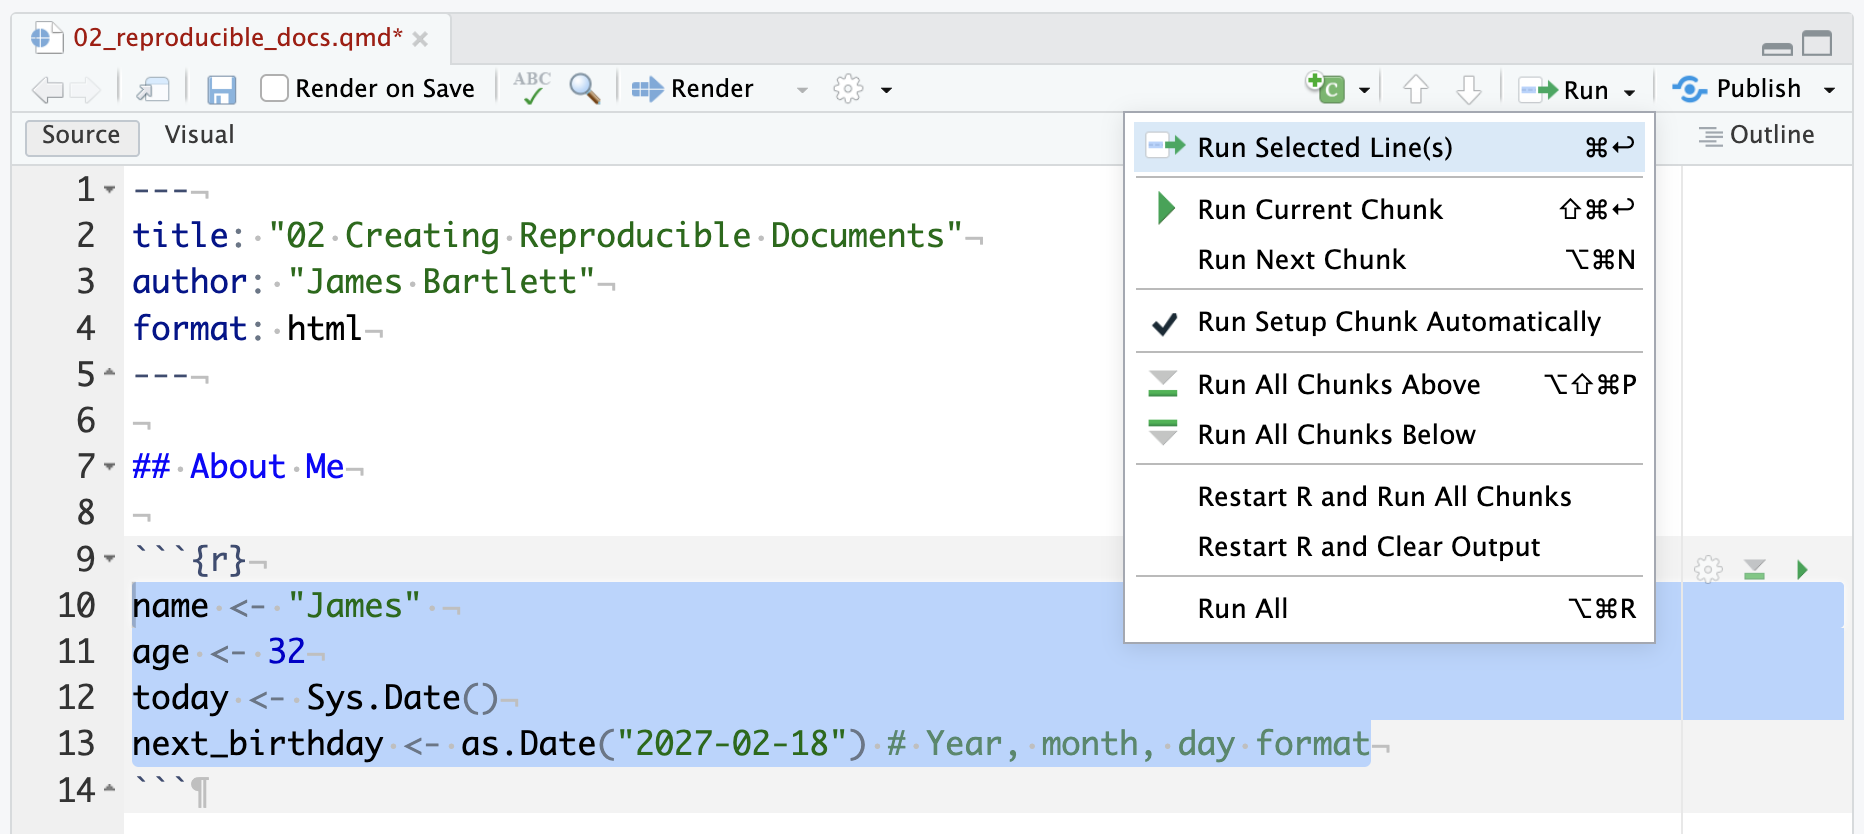
\includegraphics[width=1\textwidth,height=\textheight]{images/run1.png}

}

\caption{\label{fig-img-run1}Slower method of running code by
highlighting and clicking Run Selected Line(s).}

\end{figure}%

\begin{enumerate}
\def\labelenumi{\arabic{enumi}.}
\setcounter{enumi}{1}
\tightlist
\item
  You can press the green ``play'' button at the top-right of the code
  chunk and this will run \textbf{all} lines of code in that chunk
  (Figure~\ref{fig-img-run2}).
\end{enumerate}

\begin{figure}

\centering{

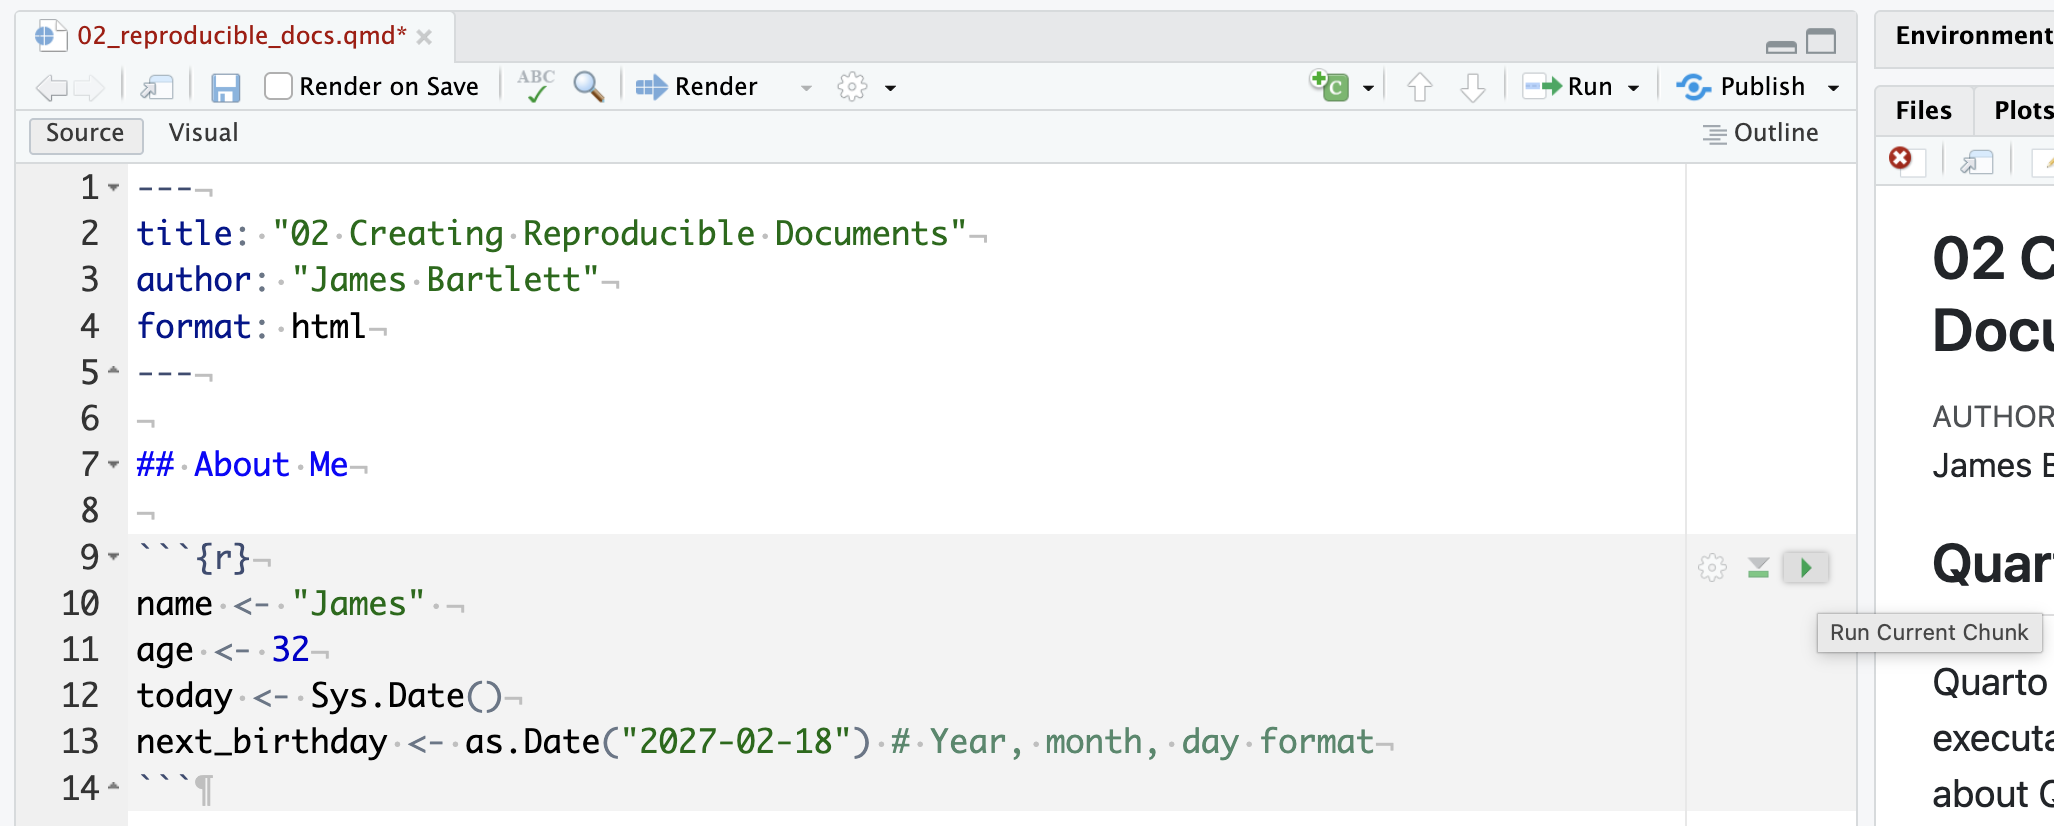
\includegraphics[width=1\textwidth,height=\textheight]{images/run2.png}

}

\caption{\label{fig-img-run2}Slightly faster method of running all code
in a chunk by clicking the green ``play'' button.}

\end{figure}%

\begin{enumerate}
\def\labelenumi{\arabic{enumi}.}
\setcounter{enumi}{2}
\tightlist
\item
  There are keyboard shortcuts to run code which will be the fastest as
  you learn and use RStudio more frequently. For example, to run a
  single line of code, make sure that the cursor is in the line of code
  (it can be anywhere on the line) you want to run and press
  \texttt{ctrl\ +\ enter} (\texttt{command\ +\ return} on a Mac).
\end{enumerate}

\begin{tcolorbox}[enhanced jigsaw, breakable, colframe=quarto-callout-note-color-frame, arc=.35mm, opacitybacktitle=0.6, titlerule=0mm, colbacktitle=quarto-callout-note-color!10!white, colback=white, toprule=.15mm, bottomtitle=1mm, toptitle=1mm, title=\textcolor{quarto-callout-note-color}{\faInfo}\hspace{0.5em}{Keyboard shortcuts}, bottomrule=.15mm, rightrule=.15mm, leftrule=.75mm, coltitle=black, left=2mm, opacityback=0]

There are loads of keyboard shortcuts, but you might only use a handful
to speed up your day-to-day tasks. For a full list, look in the top menu
\texttt{Help\ \textgreater{}\textgreater{}\ Keyboard\ shortcuts\ help}.

\end{tcolorbox}

Now run your code using one of the methods above. You should see the
variables \texttt{name}, \texttt{age}, \texttt{today}, and
\texttt{next\_birthday} appear in the environment pane in the top right
corner.

\begin{tcolorbox}[enhanced jigsaw, breakable, colframe=quarto-callout-tip-color-frame, arc=.35mm, opacitybacktitle=0.6, titlerule=0mm, colbacktitle=quarto-callout-tip-color!10!white, colback=white, toprule=.15mm, bottomtitle=1mm, toptitle=1mm, title=\textcolor{quarto-callout-tip-color}{\faLightbulb}\hspace{0.5em}{Try this}, bottomrule=.15mm, rightrule=.15mm, leftrule=.75mm, coltitle=black, left=2mm, opacityback=0]

Clear out the \hyperref[look-env]{environment using the broom handle
approach} we saw in Chapter 1 and try a different method to see which
works best for you.

\end{tcolorbox}

\subsection{Activity 7: Inline code}\label{intro-a7}

Your code works and you now know how to run it, but one of the
incredible benefits we said about R Markdown is that you can mix text
and code. Even better is the ability to combine code with text to put
specific outputs of your code, like a value, using \textbf{inline code}.

Think about a time you have had to copy and paste a value or text from
one file into another and you will know how easy it can be to make
mistakes or find the origin of your mistake. Inline code avoids this. It
is easier to show you what inline code does rather than to explain it so
let us have a go.

First, copy and paste this text exactly (do not change \emph{anything})
to underneath and outside your code chunk:

\begin{Shaded}
\begin{Highlighting}[]
\NormalTok{My name is }\StringTok{\textasciigrave{}}\AttributeTok{r name}\StringTok{\textasciigrave{}}\NormalTok{ and I am }\StringTok{\textasciigrave{}}\AttributeTok{r age}\StringTok{\textasciigrave{}}\NormalTok{ years old. }

\NormalTok{It is }\StringTok{\textasciigrave{}}\AttributeTok{r next\_birthday {-} today}\StringTok{\textasciigrave{}}\NormalTok{ days until my birthday.}
\end{Highlighting}
\end{Shaded}

Your .Rmd should look like Figure~\ref{fig-img-aboutme-rmd} but nothing
will happen yet. Unlike code chunks, you cannot run inline code. You
need to knit your document for it to do it's magic.

\begin{figure}

\centering{


\includegraphics[width=1\textwidth,height=\textheight]{images/Rmd_about_me.png}

}

\caption{\label{fig-img-aboutme-rmd}Complete .Rmd file with your about
me section and inline code.}

\end{figure}%

\begin{tcolorbox}[enhanced jigsaw, breakable, colframe=quarto-callout-note-color-frame, arc=.35mm, opacitybacktitle=0.6, titlerule=0mm, colbacktitle=quarto-callout-note-color!10!white, colback=white, toprule=.15mm, bottomtitle=1mm, toptitle=1mm, title=\textcolor{quarto-callout-note-color}{\faInfo}\hspace{0.5em}{How does inline code work?}, bottomrule=.15mm, rightrule=.15mm, leftrule=.75mm, coltitle=black, left=2mm, opacityback=0]

Inline code has the following form:

\begin{Shaded}
\begin{Highlighting}[]
\StringTok{\textasciigrave{}}\AttributeTok{r object}\StringTok{\textasciigrave{}}
\end{Highlighting}
\end{Shaded}

or

\begin{Shaded}
\begin{Highlighting}[]
\StringTok{\textasciigrave{}}\AttributeTok{r function(...)}\StringTok{\textasciigrave{}}
\end{Highlighting}
\end{Shaded}

Here, we are using the first version where we are referencing an object
we already created. This is normally a good idea if you have a long
function to run as it's easier to spot mistakes in a code chunk than
inline code.

You will see it has the form of a backtick (\texttt{\textasciigrave{}}),
\texttt{r} and a space, the object/function you want to reference, and a
final backtick. When the R Markdown file knits, it sees the \texttt{r}
and recognises it as inline code and uses the object or function.

If you just write the two backticks without the \texttt{r}, it will just
add code formatting and not produce inline code.

\end{tcolorbox}

\subsection{Activity 8: Knitting your file}\label{intro-a8}

As our final step in this part, we are going to knit our file again to
see how it looks now. So, click the Knit button to regenerate your
knitted .html version.

If you look at the knitted .html document in the Viewer tab or in your
browser, you should see the sentence we copied in from Activity 7. As if
by magic, that slightly odd bit of text you copied and pasted now
appears as a normal sentence with the values pulled in from the objects
you created:

My name is \textbf{James} and I am \textbf{30} years old. It is
\textbf{-211} days until my birthday.

R Markdown is an incredibly powerful and flexible format, we wrote this
whole book using it! There are a few final things to note about knitting
that will be useful going forward for your data skills learning and
assessments:

\begin{itemize}
\item
  R Markdown will only knit if your code works. If you have an error, it
  will stop and tell you to fix the error before you can click knit and
  try again. This is a good way of checking whether you have written
  functioning code in your assessments.
\item
  When you knit an R Markdown document, it runs the code from the start
  of the document to the end in order, and in a fresh session. This
  means it cannot access your environment, just the objects you create
  within that R Markdown. One common error can be writing and running
  code as you work on the document, but the code chunks are in the wrong
  order, or you created an object in the console but not in the code
  chunks. This means R Markdown would not know the object exists yet, or
  it does not have access to it at all.
\item
  You can choose to knit to a Word document rather than HTML. This can
  be useful for sharing with others or adding further edits, but you
  might lose some functionality. By default, html looks good and is
  accessible, so that will be our default throughout this book, but look
  out for our instructions on what output format we want your
  assessments in.
\item
  You can choose to knit to PDF, however, unless you are using the
  server this requires a \textbf{LaTeX} installation and can be quite
  complicated. If you do not already know what LaTeX is and how to use
  it, we do not recommend trying to knit to PDF just yet. If you do know
  how to use LaTeX, you probably do not need us to give you
  instructions!
\end{itemize}

We will test some of these warnings in error mode in the test yourself
section, but we have one final demonstration for how R Markdown files
support reproducibility.

\section{Demonstrating
reproducibility}\label{demonstrating-reproducibility}

At the start of this chapter, we plugged the benefits of reproducible
research as the ability to produce the same result for different people
using the same software on different computers. We are going to end the
chapter on a demonstration of this by giving you an R Markdown document
and data. You should be able to click knit and see the results without
editing anything. We do not expect you to understand the code included
in it, we are previewing the skills you will develop over the next four
chapters on visualisation and data wrangling.

\subsection{Activity 9 - Knit the reproducibility demonstration
document}\label{activity-9---knit-the-reproducibility-demonstration-document}

Please follow these steps and you should be able to knit the document
without editing anything. Make sure you are still in your
\texttt{Chapter\_02\_reproducible\_docs} folder. If you are coming back
to this activity, remember to set your working directory by opening the
.Rproj file.

\begin{enumerate}
\def\labelenumi{\arabic{enumi}.}
\item
  If you are working on your own computer, make sure you installed the
  \texttt{tidyverse} package. Please refer to
  \hyperref[install-tidy]{Chapter 1 - Activity 3} if you have not
  completed this step yet. If you are working on a university computer
  or the online server, you \textbf{do not} need to complete this step
  as \texttt{tidyverse} will already be installed.
\item
  Download the R Markdown document through the following link:
  \href{activity_files/02_reproducibility_demo.Rmd}{02\_reproducibility\_demo.Rmd}.
  To download a file from this book, right click the link and select
  ``save link as'', or just clicking the link will save the file to your
  Downloads. Save or copy the file to your
  \texttt{Chapter\_02\_reproducible\_docs} folder.
\item
  Download these two data files. Data file one:
  \href{data/ahi-cesd.csv}{ahi-cesd.csv}. Data file two:
  \href{data/participant-info.csv}{participant-info.csv}. Right click
  the links and select ``save link as'', or clicking the links will save
  the files to your Downloads. Make sure that both files are saved as
  ``.csv''. Do not open them on your machine as often other software
  like Excel can change setting and ruin the files. Save or copy the
  file to your \texttt{data/} folder within
  \texttt{Chapter\_02\_reproducible\_docs}.
\end{enumerate}

At this point, you should have
``\textbf{02\_reproducibility\_demo.Rmd}'' within your
\texttt{Chapter\_02\_reproducible\_docs} folder. You should have
``\textbf{ahi-cesd.csv}'' and ``\textbf{participant\_info.csv}'' in the
\texttt{data/} folder within \texttt{Chapter\_02\_reproducible\_docs}.

If you open ``02\_reproducibility\_demo.Rmd'' and followed all the steps
above, you should be able to click knit. This will turn the R Markdown
file into a knitted html file, showing some data wrangling, summary
statistics, and two graphs (Figure~\ref{fig-img-repro-demo}). In the
next chapter, you will learn how to write this code yourself, starting
with creating graphs.

\begin{figure}

\begin{minipage}{0.50\linewidth}

\includegraphics{images/repro_demo_Rmd.png}\end{minipage}%
%
\begin{minipage}{0.50\linewidth}
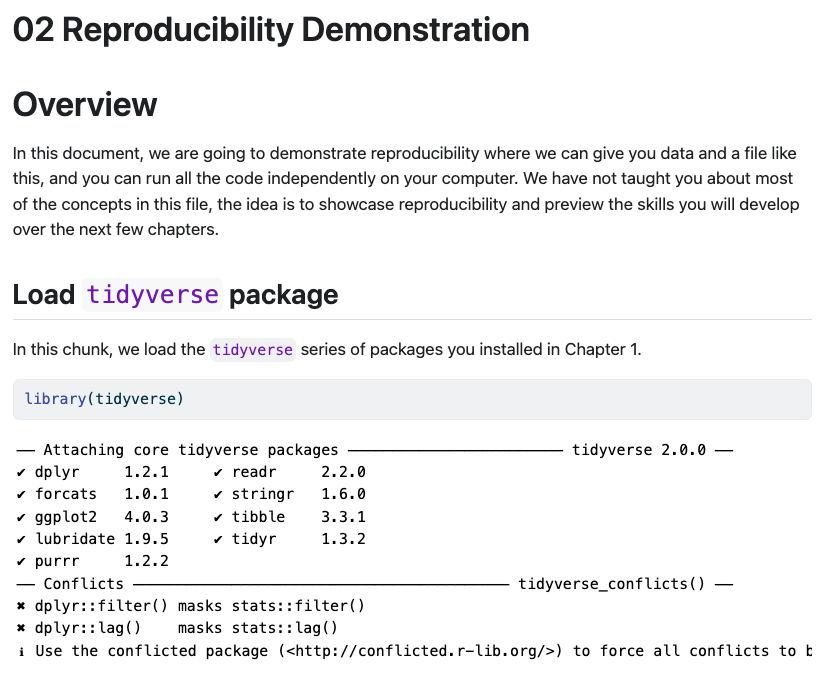
\includegraphics{images/repro_demo_html.png}\end{minipage}%

\caption{\label{fig-img-repro-demo}You should see the reproducibility
demonstration as the .Rmd (left) and be able to knit it into a html file
(right).}

\end{figure}%

If you have any questions or problems about anything contained in this
chapter, please remember you are always welcome to post on the course
Teams channel, attend a GTA support session, or attend the office hours
of one of the team.

\section{Test yourself}\label{test-yourself-1}

To end the chapter, we have some knowledge check questions to test your
understanding of the concepts we covered in the chapter. We then have
some error mode tasks to see if you can find the solution to some common
errors in the concepts we covered in this chapter.

\subsection{Knowledge check}\label{knowledge-check-1}

\textbf{Question 1}. One of the key first steps when we open RStudio is
to:

\begin{itemize}
\tightlist
\item
  \begin{enumerate}
  \def\labelenumi{(\Alph{enumi})}
  \tightlist
  \item
    set your working directory/open a project\\
  \end{enumerate}
\item
  \begin{enumerate}
  \def\labelenumi{(\Alph{enumi})}
  \setcounter{enumi}{1}
  \tightlist
  \item
    put on some music as we will be here a while\\
  \end{enumerate}
\item
  \begin{enumerate}
  \def\labelenumi{(\Alph{enumi})}
  \setcounter{enumi}{2}
  \tightlist
  \item
    check out the news\\
  \end{enumerate}
\item
  \begin{enumerate}
  \def\labelenumi{(\Alph{enumi})}
  \setcounter{enumi}{3}
  \tightlist
  \item
    make a coffee
  \end{enumerate}
\end{itemize}

\begin{tcolorbox}[enhanced jigsaw, breakable, colframe=quarto-callout-caution-color-frame, arc=.35mm, opacitybacktitle=0.6, titlerule=0mm, colbacktitle=quarto-callout-caution-color!10!white, colback=white, toprule=.15mm, bottomtitle=1mm, toptitle=1mm, title=\textcolor{quarto-callout-caution-color}{\faFire}\hspace{0.5em}{Explain this answer}, bottomrule=.15mm, rightrule=.15mm, leftrule=.75mm, coltitle=black, left=2mm, opacityback=0]

One of the most common issues we see where code does not work the first
time is because people have forgotten to set the working directory. The
working directory is the starting folder on your computer where you want
to save any files, any output, or contains your data. R/RStudio needs to
know where you want it to look, so you must either manually set your
working directory, or open a .Rproj file.

\end{tcolorbox}

\textbf{Question 2}. When using the default environment color settings
for RStudio, what color would the background of a code chunk be in R
Markdown?

\begin{itemize}
\tightlist
\item
  \begin{enumerate}
  \def\labelenumi{(\Alph{enumi})}
  \tightlist
  \item
    white\\
  \end{enumerate}
\item
  \begin{enumerate}
  \def\labelenumi{(\Alph{enumi})}
  \setcounter{enumi}{1}
  \tightlist
  \item
    red\\
  \end{enumerate}
\item
  \begin{enumerate}
  \def\labelenumi{(\Alph{enumi})}
  \setcounter{enumi}{2}
  \tightlist
  \item
    green\\
  \end{enumerate}
\item
  \begin{enumerate}
  \def\labelenumi{(\Alph{enumi})}
  \setcounter{enumi}{3}
  \tightlist
  \item
    grey
  \end{enumerate}
\end{itemize}

\textbf{Question 3}. When using the default environment color settings
for RStudio, what color would the background of normal text be in R
Markdown?

\begin{itemize}
\tightlist
\item
  \begin{enumerate}
  \def\labelenumi{(\Alph{enumi})}
  \tightlist
  \item
    white\\
  \end{enumerate}
\item
  \begin{enumerate}
  \def\labelenumi{(\Alph{enumi})}
  \setcounter{enumi}{1}
  \tightlist
  \item
    red\\
  \end{enumerate}
\item
  \begin{enumerate}
  \def\labelenumi{(\Alph{enumi})}
  \setcounter{enumi}{2}
  \tightlist
  \item
    green\\
  \end{enumerate}
\item
  \begin{enumerate}
  \def\labelenumi{(\Alph{enumi})}
  \setcounter{enumi}{3}
  \tightlist
  \item
    grey
  \end{enumerate}
\end{itemize}

\begin{tcolorbox}[enhanced jigsaw, breakable, colframe=quarto-callout-caution-color-frame, arc=.35mm, opacitybacktitle=0.6, titlerule=0mm, colbacktitle=quarto-callout-caution-color!10!white, colback=white, toprule=.15mm, bottomtitle=1mm, toptitle=1mm, title=\textcolor{quarto-callout-caution-color}{\faFire}\hspace{0.5em}{Explain this answer}, bottomrule=.15mm, rightrule=.15mm, leftrule=.75mm, coltitle=black, left=2mm, opacityback=0]

Assuming you have not changed any of the settings in RStudio, code
chunks will tend to have a grey background and normal text will tend to
have a white background. This is a good way to check that you have
closed and opened code chunks correctly.

\end{tcolorbox}

\textbf{Question 4}. Code chunks start and end with:

\begin{itemize}
\tightlist
\item
  \begin{enumerate}
  \def\labelenumi{(\Alph{enumi})}
  \tightlist
  \item
    three single quotes\\
  \end{enumerate}
\item
  \begin{enumerate}
  \def\labelenumi{(\Alph{enumi})}
  \setcounter{enumi}{1}
  \tightlist
  \item
    three backticks\\
  \end{enumerate}
\item
  \begin{enumerate}
  \def\labelenumi{(\Alph{enumi})}
  \setcounter{enumi}{2}
  \tightlist
  \item
    three double quotes\\
  \end{enumerate}
\item
  \begin{enumerate}
  \def\labelenumi{(\Alph{enumi})}
  \setcounter{enumi}{3}
  \tightlist
  \item
    three single clefs
  \end{enumerate}
\end{itemize}

\begin{tcolorbox}[enhanced jigsaw, breakable, colframe=quarto-callout-caution-color-frame, arc=.35mm, opacitybacktitle=0.6, titlerule=0mm, colbacktitle=quarto-callout-caution-color!10!white, colback=white, toprule=.15mm, bottomtitle=1mm, toptitle=1mm, title=\textcolor{quarto-callout-caution-color}{\faFire}\hspace{0.5em}{Explain this answer}, bottomrule=.15mm, rightrule=.15mm, leftrule=.75mm, coltitle=black, left=2mm, opacityback=0]

Code chunks always take the same general format of three backticks
followed by curly parentheses and a lower case r inside the parentheses
(\texttt{\{r\}}). People often mistake these backticks for single quotes
but that will not work. If you have set your code chunk correctly using
backticks, the background color should change to grey from white

\end{tcolorbox}

\textbf{Question 5}. Inline code is:

\begin{itemize}
\tightlist
\item
  \begin{enumerate}
  \def\labelenumi{(\Alph{enumi})}
  \tightlist
  \item
    where you nicely organise your code in a line.\\
  \end{enumerate}
\item
  \begin{enumerate}
  \def\labelenumi{(\Alph{enumi})}
  \setcounter{enumi}{1}
  \tightlist
  \item
    where you make sure all the code is nicely indented from the side.\\
  \end{enumerate}
\item
  \begin{enumerate}
  \def\labelenumi{(\Alph{enumi})}
  \setcounter{enumi}{2}
  \tightlist
  \item
    a fancy way of saying you have written good code.\\
  \end{enumerate}
\item
  \begin{enumerate}
  \def\labelenumi{(\Alph{enumi})}
  \setcounter{enumi}{3}
  \tightlist
  \item
    an approach of integrating code and text in a sentence outside of a
    code chunk.
  \end{enumerate}
\end{itemize}

\begin{tcolorbox}[enhanced jigsaw, breakable, colframe=quarto-callout-caution-color-frame, arc=.35mm, opacitybacktitle=0.6, titlerule=0mm, colbacktitle=quarto-callout-caution-color!10!white, colback=white, toprule=.15mm, bottomtitle=1mm, toptitle=1mm, title=\textcolor{quarto-callout-caution-color}{\faFire}\hspace{0.5em}{Explain this answer}, bottomrule=.15mm, rightrule=.15mm, leftrule=.75mm, coltitle=black, left=2mm, opacityback=0]

Inline coding is an incredibly useful approach for merging text and code
in a sentence outside of a code chunk. It can be really useful for when
you want to add values from your code directly into your text. If you
copy and paste values, you can easily create errors, so it's useful to
add inline code where possible.

\end{tcolorbox}

\subsection{Error mode}\label{error-mode-4}

The following questions are designed to introduce you to making and
fixing errors. For this topic, we focus on R Markdown and potential
errors in using code blocks and inline code. Remember to keep a note of
what kind of error messages you receive and how you fixed them, so you
have a bank of solutions when you tackle errors independently.

Create and save a new R Markdown file by following the instructions in
\hyperref[intro-a3]{activity 3} and \hyperref[intro-a4]{activity 4}. You
should have a blank R Markdown file below line 10. Below, we have
several variations of a code chunk and inline code errors. Copy and
paste them into your R Markdown file, click knit, and look at the error
message you receive. See if you can fix the error and get it working
before checking the answer.

\textbf{Note}: For all of our error mode activities, the error is based
on clicking knit so it applies to inline code examples. If you try and
run the code instead of clicking knit on the whole document, you might
see a different error message to what we report.

\textbf{Question 6}. Copy the following text/code/code chunk into your R
Markdown file and press knit. You should receive an error like
\texttt{Line\ 18\ Execution\ halted} in the Render tab.

\begin{Shaded}
\begin{Highlighting}[]
\NormalTok{city \textless{}{-} "Glasgow"}

\InformationTok{\textasciigrave{}\textasciigrave{}\textasciigrave{}\{r\}}

\InformationTok{\textasciigrave{}\textasciigrave{}\textasciigrave{}}
\InformationTok{\textasciigrave{}r city\textasciigrave{}}\NormalTok{ is a city in Scotland. }
\end{Highlighting}
\end{Shaded}

\begin{tcolorbox}[enhanced jigsaw, breakable, colframe=quarto-callout-caution-color-frame, arc=.35mm, opacitybacktitle=0.6, titlerule=0mm, colbacktitle=quarto-callout-caution-color!10!white, colback=white, toprule=.15mm, bottomtitle=1mm, toptitle=1mm, title=\textcolor{quarto-callout-caution-color}{\faFire}\hspace{0.5em}{Explain the solution}, bottomrule=.15mm, rightrule=.15mm, leftrule=.75mm, coltitle=black, left=2mm, opacityback=0]

Here, we wrote \texttt{city\ \textless{}-\ "Glasgow"} outside the code
chunk. So, when we try and knit, it is not evaluated as code, and city
does not exist as an object to be referenced in inline code. If you copy
\texttt{city\ \textless{}-\ "Glasgow"} into the code chunk and press
knit, it should work.

\end{tcolorbox}

\textbf{Question 7}. Copy the following text/code/code chunk into your R
Markdown file and press knit. You should receive an error like
\texttt{Error\ in\ parse():\ !\ attempt\ to\ use\ zero-length\ variable\ name}
which is not very helpful for diagnosing the problem.

\begin{Shaded}
\begin{Highlighting}[]

\InformationTok{\textasciigrave{}\textasciigrave{}\textasciigrave{}\{r\}}
\InformationTok{city \textless{}{-} "Glasgow"}
\InformationTok{\textasciigrave{}\textasciigrave{}}

\InformationTok{\textasciigrave{}r city\textasciigrave{} is a city in Scotland. }
\end{Highlighting}
\end{Shaded}

\begin{tcolorbox}[enhanced jigsaw, breakable, colframe=quarto-callout-caution-color-frame, arc=.35mm, opacitybacktitle=0.6, titlerule=0mm, colbacktitle=quarto-callout-caution-color!10!white, colback=white, toprule=.15mm, bottomtitle=1mm, toptitle=1mm, title=\textcolor{quarto-callout-caution-color}{\faFire}\hspace{0.5em}{Explain the solution}, bottomrule=.15mm, rightrule=.15mm, leftrule=.75mm, coltitle=black, left=2mm, opacityback=0]

Here, we missed a final backtick in the code chunk. You might have
noticed all the text had a grey background, so R Markdown thought
everything was code. So, when it reached the inline code and text, it
tried interpreting it as code and caused the error. If you add the final
backtick to the code chunk, you should be able to click knit
successfully.

\end{tcolorbox}

\textbf{Question 8}. Copy the following text/code/code chunk into your R
Markdown file and press knit. You should receive an error like
\texttt{Line\ 12\ Execution\ halted} in the Render tab.

\begin{Shaded}
\begin{Highlighting}[]

\InformationTok{\textasciigrave{}r city\textasciigrave{}}\NormalTok{ is a city in Scotland. }

\InformationTok{\textasciigrave{}\textasciigrave{}\textasciigrave{}\{r\}}
\InformationTok{city \textless{}{-} "Glasgow"}
\InformationTok{\textasciigrave{}\textasciigrave{}\textasciigrave{}}
\end{Highlighting}
\end{Shaded}

\begin{tcolorbox}[enhanced jigsaw, breakable, colframe=quarto-callout-caution-color-frame, arc=.35mm, opacitybacktitle=0.6, titlerule=0mm, colbacktitle=quarto-callout-caution-color!10!white, colback=white, toprule=.15mm, bottomtitle=1mm, toptitle=1mm, title=\textcolor{quarto-callout-caution-color}{\faFire}\hspace{0.5em}{Explain the solution}, bottomrule=.15mm, rightrule=.15mm, leftrule=.75mm, coltitle=black, left=2mm, opacityback=0]

Here, we tried using inline code before the code chunk. R Markdown runs
the code from start to finish in a fresh environment. We tried
referencing \texttt{city} in inline code, but R Markdown did not know it
existed yet. To fix it, you need to move the inline code below the code
chunk, so you create \texttt{city} before referencing it in inline code.

\end{tcolorbox}

\textbf{Question 9}. Copy the following text/code/code chunk into your R
Markdown file and press knit. This\ldots works?

\begin{Shaded}
\begin{Highlighting}[]

\InformationTok{\textasciigrave{}\textasciigrave{}\textasciigrave{}\{r\}}
\InformationTok{city \textless{}{-} "Glasgow"}
\InformationTok{\textasciigrave{}\textasciigrave{}\textasciigrave{}}

\InformationTok{\textasciigrave{}city\textasciigrave{}}\NormalTok{ is a city in Scotland. }
\end{Highlighting}
\end{Shaded}

\begin{tcolorbox}[enhanced jigsaw, breakable, colframe=quarto-callout-caution-color-frame, arc=.35mm, opacitybacktitle=0.6, titlerule=0mm, colbacktitle=quarto-callout-caution-color!10!white, colback=white, toprule=.15mm, bottomtitle=1mm, toptitle=1mm, title=\textcolor{quarto-callout-caution-color}{\faFire}\hspace{0.5em}{Explain the solution}, bottomrule=.15mm, rightrule=.15mm, leftrule=.75mm, coltitle=black, left=2mm, opacityback=0]

Here, we have a sneaky kind of ``error'' where it knits, but it is not
doing what we wanted it to do. In the inline code part, we only added
code formatting \texttt{city}, we did not add the r to get R Markdown to
interpret it as R code:

\begin{Shaded}
\begin{Highlighting}[]
\StringTok{\textasciigrave{}}\AttributeTok{r city}\StringTok{\textasciigrave{}}
\end{Highlighting}
\end{Shaded}

If you add the \texttt{r} after the first backtick, it should knit and
add the city object in.

\end{tcolorbox}

\section{Words from this Chapter}\label{words-from-this-chapter-1}

Below, you will find a list of words that we used in this chapter that
might be new to you in case you need to refer back to what they mean.
The links in this table take you to the entry for the words in the
\href{https://psyteachr.github.io/glossary/}{PsyTeachR Glossary}. Note
that numerous members of the team wrote entries in the Glossary and as
such the entries may use slightly different terminology from what we
used in the chapter.

\begin{longtable}[]{@{}
  >{\raggedright\arraybackslash}p{(\columnwidth - 2\tabcolsep) * \real{0.2333}}
  >{\raggedright\arraybackslash}p{(\columnwidth - 2\tabcolsep) * \real{0.7667}}@{}}
\toprule\noalign{}
\begin{minipage}[b]{\linewidth}\raggedright
term
\end{minipage} & \begin{minipage}[b]{\linewidth}\raggedright
definition
\end{minipage} \\
\midrule\noalign{}
\endhead
\bottomrule\noalign{}
\endlastfoot
\href{https://psyteachr.github.io/glossary/c\#chunk}{chunk} & A section
of code in an R Markdown file \\
\href{https://psyteachr.github.io/glossary/h\#html}{html} & Hyper-Text
Markup Language: A system for semantically tagging structure and
information on web pages. \\
\href{https://psyteachr.github.io/glossary/i\#inline-code}{inline-code}
& Directly inserting the result of code into the text of a .Rmd file. \\
\href{https://psyteachr.github.io/glossary/k\#knit}{knit} & To create an
HTML, PDF, or Word document from an R Markdown (Rmd) document \\
\href{https://psyteachr.github.io/glossary/l\#latex}{latex} & A
typesetting program needed to create PDF files from R Markdown
documents. \\
\href{https://psyteachr.github.io/glossary/m\#markdown}{markdown} & A
way to specify formatting, such as headers, paragraphs, lists, bolding,
and links. \\
\href{https://psyteachr.github.io/glossary/r\#r-markdown}{r-markdown} &
The R-specific version of markdown: a way to specify formatting, such as
headers, paragraphs, lists, bolding, and links, as well as code blocks
and inline code. \\
\href{https://psyteachr.github.io/glossary/r\#r-project}{r-project} & A
project is simply a working directory designated with a .RProj file.
When you open an R project, it automatically sets the working directory
to the folder the project is located in. \\
\href{https://psyteachr.github.io/glossary/r\#reproducible-research}{reproducible-research}
& Research that documents all of the steps between raw data and results
in a way that can be verified. \\
\href{https://psyteachr.github.io/glossary/w\#working-directory}{working-directory}
& The filepath where R is currently loading files from and saving files
to. \\
\end{longtable}

\section{End of chapter}\label{end-of-chapter-1}

Well done on reaching the end of the second chapter! This was another
long chapter as we had to cover a range of foundational skills to
prepare you for learning more of the coding element in future chapters.

The next chapter builds on all the skills you have developed so far in R
programming and creating reproducible documents to focus on something
more tangible: data visualisation in R to create plots of your data.

\bookmarksetup{startatroot}

\chapter{Introduction to Data Visualisation}\label{c03-intro-data-viz}

In this chapter, we introduce you to data visualisation. Visualising our
data and the relationships between our variables is an incredibly useful
and important skill.

It is important for \textbf{you} before you conduct any statistical
analyses or present any summary statistics. We should always visualise
our data as it is a quick and easy way to check our data make sense and
identify any unusual trends. It is also important for \textbf{others}
who read your work. Data visualisation can honestly present the features
of our data to anyone who reads our research and provides a faster
overview of our findings than reading a wall of numbers.

Across several chapters, we introduce you to the extremely flexible
\texttt{ggplot2} package for data visualisation as part of the
\texttt{tidyverse} family. In two or three lines of code, you can create
plots like Figure~\ref{fig-ggplotdemo} for exploratory data analysis.
With a few extra lines, you can create publication quality plots that
could go into a report.

In this chapter, we introduce you to the \texttt{ggplot2} system of
creating plots and cover histograms and bar plots. In future chapters,
we cover different types of plot to communicate more complex data and
analyses.

\textbf{Chapter Intended Learning Outcomes (ILOs)}

By the end of this chapter, you will be able to:

\begin{itemize}
\item
  Read data files into R/RStudio.
\item
  Understand the \texttt{ggplot2} layering system of creating plots.
\item
  Create and edit histograms to visualise the frequency of observations
  collated into bins.
\item
  Create and edit barplots to visualise the frequency of different
  categories.
\item
  Save plots as an image to use in reports or presentations.
\end{itemize}

\begin{figure}

\centering{

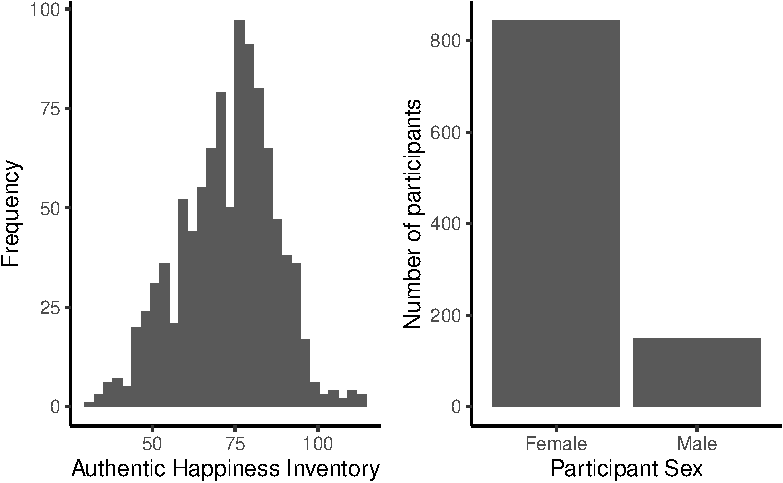
\includegraphics[width=1\textwidth,height=\textheight]{03-intro-data-viz_files/figure-pdf/fig-ggplotdemo-1.pdf}

}

\caption{\label{fig-ggplotdemo}Preview of the kind of plots you can
quickly create using the ggplot2 package. On the left, a histogram of
responses to a happiness questionnaire. On the right, a bar plot showing
the frequency men and women in the study.}

\end{figure}%

\section{Chapter preparation}\label{chapter-preparation}

\subsection{Introduction to the data
set}\label{introduction-to-the-data-set}

From now on, we are going to use different data sets from psychology to
develop and practice your data skills. This will prepare you for working
with different kinds of psychology data and introduce you to different
kinds of research questions they might ask. For this chapter, we are
using open data from Woodworth et al. (2018). The abstract of their
article is:

\begin{quote}
We present two datasets. The first dataset comprises 992 point-in-time
records of self-reported happiness and depression in 295 participants,
each assigned to one of four intervention groups, in a study of the
effect of web-based positive-psychology interventions. Each
point-in-time measurement consists of a participant's responses to the
24 items of the Authentic Happiness Inventory and to the 20 items of the
Center for Epidemiological Studies Depression (CES-D) scale.
Measurements were sought at the time of each participant's enrolment in
the study and on five subsequent occasions, the last being approximately
189 days after enrolment. The second dataset contains basic demographic
information about each participant.
\end{quote}

In summary, we have two files containing demographic information about
participants and measurements of two scales on happiness and depression:

\begin{itemize}
\item
  The Authentic Happiness Inventory (AHI),
\item
  The Center for Epidemiological Studies Depression (CES-D) scale.
\end{itemize}

\subsection{Organising your files and project for the
chapter}\label{organising-your-files-and-project-for-the-chapter}

Before we can get started, you need to organise your files and project
for the chapter, so your working directory is in order. If you need a
refresher of this process, you can look back over Chapter 2 -
\hyperref[02-projects]{File structure, working directories, and R
Projects}.

\begin{enumerate}
\def\labelenumi{\arabic{enumi}.}
\item
  In your folder for research methods and the book
  \texttt{ResearchMethods1\_2/Quant\_Fundamentals}, create a new folder
  called \texttt{Chapter\_03\_intro\_data\_viz}. Within
  \texttt{Chapter\_03\_intro\_data\_viz}, create two new folders called
  \texttt{data} and \texttt{figures}.
\item
  Create an R Project for \texttt{Chapter\_03\_intro\_data\_viz} as an
  existing directory for your chapter folder. This should now be your
  working directory.
\item
  Create a new R Markdown document and give it a sensible title
  describing the chapter, such as
  \texttt{03\ Introduction\ to\ Data\ Visualisation}. Delete everything
  below line 10 so you have a blank file to work with and save the file
  in your \texttt{Chapter\_03\_intro\_data\_viz} folder.
\item
  Download these two data files which we used at the end of Chapter 2.
  Data file one: \href{data/ahi-cesd.csv}{ahi-cesd.csv}. Data file two:
  \href{data/participant-info.csv}{participant-info.csv}. Right click
  the links and select ``save link as'', or clicking the links will save
  the files to your Downloads. Make sure that both files are saved as
  ``.csv''. Do not open them on your machine as often other software
  like Excel can change setting and ruin the files. Save or copy the
  file to your \texttt{data/} folder within
  \texttt{Chapter\_03\_intro\_data\_viz}.
\end{enumerate}

You are now ready to start working on the chapter!

\begin{tcolorbox}[enhanced jigsaw, breakable, colframe=quarto-callout-note-color-frame, arc=.35mm, opacitybacktitle=0.6, titlerule=0mm, colbacktitle=quarto-callout-note-color!10!white, colback=white, toprule=.15mm, bottomtitle=1mm, toptitle=1mm, title=\textcolor{quarto-callout-note-color}{\faInfo}\hspace{0.5em}{Reminder of file management if you use the online server}, bottomrule=.15mm, rightrule=.15mm, leftrule=.75mm, coltitle=black, left=2mm, opacityback=0]

If we support you to use the online University of Glasgow R Server,
working with files is a little different. If you downloaded R / RStudio
to your own computer or you are using one of the library/lab computers,
please ignore this section.

The main disadvantage to using the R server is that you will need create
folders on the server and then upload and download any files you are
working on to and from the server. Please be aware that \textbf{there is
no link between your computer and the R server}. If you change files on
the server, they will not appear on your computer until you download
them from the server, and you need to be very careful when you submit
your assessment files that you are submitting the right file. This is
the main reason we recommend installing R / RStudio on your computer
wherever possible.

Going forward throughout this book, if you are using the server, you
will need to follow an extra step where you also upload them to the
sever. As an example:

\begin{enumerate}
\def\labelenumi{\arabic{enumi}.}
\item
  Log on to the \textbf{R server} using the link we provided to you.
\item
  In the file pane, click \texttt{New\ folder} and create the same
  structure we demonstrated above.
\item
  Download these two data files which we used at the end of Chapter 2.
  Data file one: \href{data/ahi-cesd.csv}{ahi-cesd.csv}. Data file two:
  \href{data/participant_info.csv}{participant-info.csv}. Save the two
  files into the \texttt{data} folder you created for chapter 3. To
  download a file from this book, right click the link and select ``save
  link as''. Make sure that both files are saved as ``.csv''. Do not
  open them on your machine as often other software like Excel can
  change setting and ruin the files.
\item
  Now that the files are stored on your computer, go to RStudio on the
  server and click \texttt{Upload} then \texttt{Browse} and choose the
  folder for the chapter you are working on.
\item
  Click \texttt{Choose\ file} and go and find the data you want to
  upload.
\end{enumerate}

\end{tcolorbox}

\section{\texorpdfstring{Loading the \texttt{tidyverse} and reading data
files}{Loading the tidyverse and reading data files}}\label{loading-the-tidyverse-and-reading-data-files}

\subsection{\texorpdfstring{Activity 1 - Loading the \texttt{tidyverse}
package}{Activity 1 - Loading the tidyverse package}}\label{activity-1---loading-the-tidyverse-package}

For everything we do in this chapter and almost every chapter from now,
we need to use the \textbf{tidyverse} package. The \texttt{tidyverse} is
a package of packages, containing a kind of ecosystem of functions that
work together for \textbf{data wrangling}, \textbf{descriptive}
statistics, and visualisation. So let's load that package into our
library using the \texttt{library()} function.

To load the \texttt{tidyverse}, below line 10 of your RMarkdown
document, create a code chunk, type the following code into your code
chunk, and run the code:

\begin{Shaded}
\begin{Highlighting}[]
\FunctionTok{library}\NormalTok{(tidyverse)}
\end{Highlighting}
\end{Shaded}

Remember that sometimes in the \textbf{console} or below your code
chunk, you will see information about the package you have loaded. If
you see an error message, be sure to read it and try to identify what
the problem is. For example, if you are working on your own computer,
have you installed \texttt{tidyverse} so R/RStudio can access it? Are
there any spelling mistakes in the function or package?

Remember though, not all messages are errors, \texttt{tidyverse}
explains what packages it loaded and highlights function name clashes.
See \hyperref[install-tidy]{activity 3} and 4 from Chapter 1 if you need
a refresher.

\subsection{\texorpdfstring{Activity 2 - Reading data files using
\texttt{read\_csv()}}{Activity 2 - Reading data files using read\_csv()}}\label{activity-2---reading-data-files-using-read_csv}

Now we have loaded \texttt{tidyverse}, we can read in the data we need
for the remaining activities. ``Read'' in this sense just means to bring
the data into RStudio and store it in an \textbf{object}, so we can work
with it.

We will use the function \texttt{read\_csv()} that allows us to read in
\textbf{.csv files}. There are also functions that allow you to read in
Excel files (e.g.~.xlsx) and other formats, but in this course we will
only use .csv files as they are not software specific, meaning they are
more accessible to share, promoting our open science principles.

\begin{tcolorbox}[enhanced jigsaw, breakable, colframe=quarto-callout-note-color-frame, arc=.35mm, opacitybacktitle=0.6, titlerule=0mm, colbacktitle=quarto-callout-note-color!10!white, colback=white, toprule=.15mm, bottomtitle=1mm, toptitle=1mm, title=\textcolor{quarto-callout-note-color}{\faInfo}\hspace{0.5em}{Where does \texttt{read\_csv()} come from?}, bottomrule=.15mm, rightrule=.15mm, leftrule=.75mm, coltitle=black, left=2mm, opacityback=0]

When we describe tidyverse as a package of packages, the
\texttt{read\_csv()} function comes from a package called
\texttt{readr}. This is one of the packages that tidyverse loads and
contains several functions for reading different kinds of data.

\end{tcolorbox}

Create a new code chunk below where you loaded \texttt{tidyverse}, type
the following code, and run the code chunk:

\begin{Shaded}
\begin{Highlighting}[]
\NormalTok{dat }\OtherTok{\textless{}{-}} \FunctionTok{read\_csv}\NormalTok{(}\StringTok{"data/ahi{-}cesd.csv"}\NormalTok{)}

\NormalTok{pinfo }\OtherTok{\textless{}{-}} \FunctionTok{read\_csv}\NormalTok{(}\StringTok{"data/participant{-}info.csv"}\NormalTok{)}
\end{Highlighting}
\end{Shaded}

To break down the code:

\begin{itemize}
\item
  First, we create an object called \texttt{dat} that contains the data
  in the \texttt{ahi-cesd.csv} file within \texttt{data/}.
\item
  Next, we create an object called \texttt{pinfo} that contains the data
  in the \texttt{participant-info.csv} file within \texttt{data/}.
\item
  Both lines have the same format of
  \texttt{object\ \textless{}-\ function("folder/datafile\_name.csv")}
\item
  Remember that \texttt{\textless{}-} is called the \textbf{assignment
  operator} but we can read it as ``assigned to''. For example, the
  first line can be read as the data in \texttt{data/ahi-cesd.csv} is
  assigned to the object called \texttt{dat}.
\end{itemize}

\begin{tcolorbox}[enhanced jigsaw, breakable, colframe=quarto-callout-important-color-frame, arc=.35mm, opacitybacktitle=0.6, titlerule=0mm, colbacktitle=quarto-callout-important-color!10!white, colback=white, toprule=.15mm, bottomtitle=1mm, toptitle=1mm, title=\textcolor{quarto-callout-important-color}{\faExclamation}\hspace{0.5em}{Error mode}, bottomrule=.15mm, rightrule=.15mm, leftrule=.75mm, coltitle=black, left=2mm, opacityback=0]

There are several common mistakes that can happen here, so be careful
how you are typing the code to read in the data.

\begin{itemize}
\item
  You need the double quotation marks around the data file name, so R
  recognises you are giving it a file path.
\item
  Computers are literal, so you must spell the data file name correctly.
  For example, R would not know what \texttt{data/participant-inf.csv}
  is. This is where pressing the tab key on your keyboard can be super
  helpful, as you can search and auto-complete your files and avoid
  spelling mistakes.
\item
  For the same reason as spelling mistakes, you must add the .csv part
  on the end to tell R the specific file you want.
\item
  You must point R to the right folder relative to your working
  directory. If you typed \texttt{ahi-cesd.csv}, you would receive an
  error as R would look in your chapter folder where
  \texttt{ahi-cesd.csv} does not exist, rather than within the
  \texttt{data/} folder you stored it in.
\end{itemize}

\end{tcolorbox}

If you have done this activity correctly, you should now see the objects
\texttt{dat} and \texttt{pinfo} in the \textbf{environment} window in
the top right of RStudio. If they are not there, check there are no
error messages, check the spelling of the code and file names, and check
your working directory is \texttt{Chapter\_03\_intro\_data\_viz}.

\begin{tcolorbox}[enhanced jigsaw, breakable, colframe=quarto-callout-warning-color-frame, arc=.35mm, opacitybacktitle=0.6, titlerule=0mm, colbacktitle=quarto-callout-warning-color!10!white, colback=white, toprule=.15mm, bottomtitle=1mm, toptitle=1mm, title=\textcolor{quarto-callout-warning-color}{\faExclamationTriangle}\hspace{0.5em}{Be careful to use the right \texttt{read\_csv()} function}, bottomrule=.15mm, rightrule=.15mm, leftrule=.75mm, coltitle=black, left=2mm, opacityback=0]

There is also a function called \texttt{read.csv()}. Be very careful
\textbf{not} to use this function instead of \texttt{read\_csv()} as
they have different ways of naming columns. For the activities and the
assignments in RM1 and RM2, we will \textbf{always} ask and expect you
to use \texttt{read\_csv()}. This is really a reminder to watch spelling
on functions and to be careful to use the right functions, especially
when the names are so close.

\end{tcolorbox}

\subsection{Activity 3 - Wrangling the two data
sets}\label{activity-3---wrangling-the-two-data-sets}

For this final preparation step, we would like you to add the following
code. We are not tackling data wrangling until the next chapter, so we
are not going to fully explain the code just yet. Copy the code (if you
hover over the code, there is a copy to clipboard icon in the top right)
and paste it into a code chunk below where you read the two data files,
then run the code again.

\begin{Shaded}
\begin{Highlighting}[]
\NormalTok{all\_dat }\OtherTok{\textless{}{-}} \FunctionTok{inner\_join}\NormalTok{(dat, }
\NormalTok{                      pinfo, }
                      \AttributeTok{by=} \FunctionTok{c}\NormalTok{(}\StringTok{"id"}\NormalTok{, }\StringTok{"intervention"}\NormalTok{))}

\NormalTok{summarydata }\OtherTok{\textless{}{-}} \FunctionTok{select}\NormalTok{(}\AttributeTok{.data =}\NormalTok{ all\_dat, }
\NormalTok{                      id,}
\NormalTok{                      occasion, }
\NormalTok{                      elapsed.days,}
\NormalTok{                      intervention,}
\NormalTok{                      ahiTotal, }
\NormalTok{                      cesdTotal, }
\NormalTok{                      sex, }
\NormalTok{                      age, }
\NormalTok{                      educ, }
\NormalTok{                      income)}
\end{Highlighting}
\end{Shaded}

For a brief overview, we are joining the two data files by common
columns (``id'' and ``intervention'') to create the object
\texttt{all\_dat}. We are then selecting 10 columns from the original 54
to make the data easier to work with in \texttt{summarydata}.

This final object \texttt{summarydata} is the source of the data we will
be working with for the rest of this chapter.

\subsection{Activity 4 - Exploring the data
set}\label{activity-4---exploring-the-data-set}

Before we start plotting, it is a good idea to explore the data set you
are working with. There is a handy function called \texttt{glimpse()}
which provides an overview of the columns and responses in your data
set.

Create a new code chunk below where you read and wrangled the data, and
type and run the following code:

\begin{Shaded}
\begin{Highlighting}[]
\FunctionTok{glimpse}\NormalTok{(summarydata)}
\end{Highlighting}
\end{Shaded}

\begin{verbatim}
Rows: 992
Columns: 10
$ id           <dbl> 12, 162, 162, 267, 126, 289, 113, 8, 185, 185, 246, 185, ~
$ occasion     <dbl> 5, 2, 3, 0, 5, 0, 2, 2, 2, 4, 4, 0, 4, 0, 1, 4, 0, 5, 4, ~
$ elapsed.days <dbl> 182.025139, 14.191806, 33.033831, 0.000000, 202.096887, 0~
$ intervention <dbl> 2, 3, 3, 4, 2, 1, 1, 2, 3, 3, 3, 3, 1, 2, 2, 2, 3, 2, 2, ~
$ ahiTotal     <dbl> 32, 34, 34, 35, 36, 37, 38, 38, 38, 38, 39, 40, 41, 41, 4~
$ cesdTotal    <dbl> 50, 49, 47, 41, 36, 35, 50, 55, 47, 39, 45, 47, 33, 27, 3~
$ sex          <dbl> 1, 1, 1, 1, 1, 1, 2, 1, 2, 2, 1, 2, 1, 2, 2, 1, 1, 1, 1, ~
$ age          <dbl> 46, 37, 37, 19, 40, 49, 42, 57, 41, 41, 52, 41, 52, 58, 5~
$ educ         <dbl> 4, 3, 3, 2, 5, 4, 4, 4, 4, 4, 5, 4, 5, 5, 5, 4, 3, 4, 3, ~
$ income       <dbl> 3, 2, 2, 1, 2, 1, 1, 2, 1, 1, 2, 1, 3, 2, 2, 3, 2, 2, 2, ~
\end{verbatim}

\begin{tcolorbox}[enhanced jigsaw, breakable, colframe=quarto-callout-note-color-frame, arc=.35mm, opacitybacktitle=0.6, titlerule=0mm, colbacktitle=quarto-callout-note-color!10!white, colback=white, toprule=.15mm, bottomtitle=1mm, toptitle=1mm, title=\textcolor{quarto-callout-note-color}{\faInfo}\hspace{0.5em}{Where does \texttt{glimpse()} come from?}, bottomrule=.15mm, rightrule=.15mm, leftrule=.75mm, coltitle=black, left=2mm, opacityback=0]

The \texttt{glimpse()} function comes from a package called
\texttt{dplyr}, which is part of the tidyverse. This package contains
many functions for wrangling data like joining data sets and selecting
columns. We will explore loads of functions within \texttt{dplyr} in the
next few chapters on data wrangling.

\end{tcolorbox}

This function provides a condensed summary of your data. You can see
there are 992 rows and 10 columns. You see all the column names for each
variable in the data set. You can also see that all the variables are
automatically considered as numeric (in this case double represented by
\texttt{\textless{}dbl\textgreater{}}). Treating categorical variables
like ``sex'' and ``income'' as numbers will cause us problems later, but
it is fine for the variables we will be working on now.

\section{\texorpdfstring{\texttt{ggplot2} and the layer
system}{ggplot2 and the layer system}}\label{ggplot2-and-the-layer-system}

There are multiple approaches to data visualisation in R but we will use
\texttt{ggplot2} which uses a layered grammar of graphics where you
build up plots in a series of layers. You can think of it as building a
picture with multiple elements that sit over each other.

Figure~\ref{fig-img-layers} from Nordmann et al. (2022) demonstrates the
idea of building up a plot by adding layers. One function creates the
first layer, the basic plot area, and you add functions and arguments to
add additional layers such as the data, the labels, the colors etc. If
you are used to making plots in other software, this might seem a bit
odd at first, but it means that you can customise each layer separately
to make complex and beautiful figures with relative ease.

You can get a sense of what plots are possible from
\href{https://www.data-to-viz.com/}{the website data-to-viz}, but we
will build up your data visualisation skills over the RM1 and RM2
courses.

\begin{figure}

\centering{


\includegraphics[width=1\textwidth,height=\textheight]{images/layers2.PNG}

}

\caption{\label{fig-img-layers}Building a figure using the ggplot2
layering system from Nordmann et al.~(2022).}

\end{figure}%

\section{Histograms and density
plots}\label{histograms-and-density-plots}

We are going to start by plotting the distribution of participant age in
a histogram, and add layers to demonstrate how we build the plot
step-by-step.

\subsection{\texorpdfstring{Step 1: Start with the \texttt{ggplot}
function}{Step 1: Start with the ggplot function}}\label{step-1-start-with-the-ggplot-function}

This first layer tells R to access the \texttt{ggplot} function.

The first argument tells R to plot the \texttt{summarydata} dataframe.
In the \texttt{aes} function, you specify the aesthetics of the plot,
such as the axes and colours. What you need to specify depends on the
plot you want to make (you will learn more about this later).

For a basic histogram, you only need to specify the x-axis (the y-axis
will automatically be counts).

For each step, type the code in a new code chunk and run it after we add
each layer to see it's effect.

\begin{Shaded}
\begin{Highlighting}[]
\CommentTok{\# Plot the variable age from summarydata}
\FunctionTok{ggplot}\NormalTok{(summarydata, }\FunctionTok{aes}\NormalTok{(}\AttributeTok{x =}\NormalTok{ age)) }\CommentTok{\# Plot age on the x axis}
\end{Highlighting}
\end{Shaded}

\begin{center}
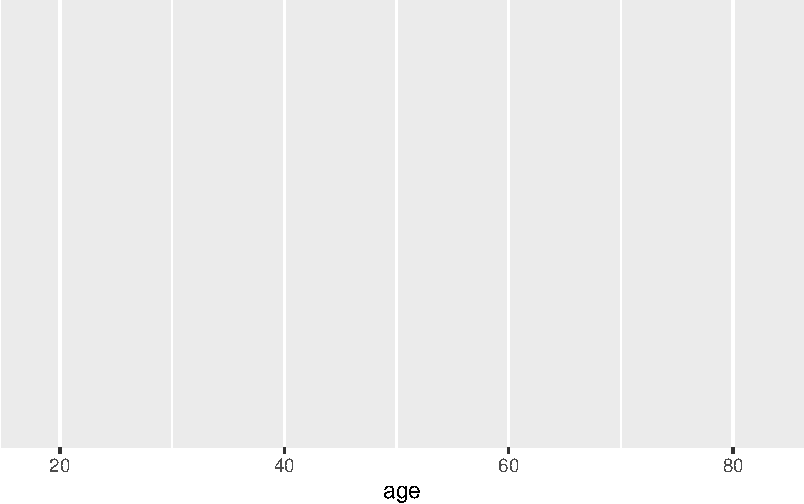
\includegraphics[width=1\textwidth,height=\textheight]{03-intro-data-viz_files/figure-pdf/histogram1-1.pdf}
\end{center}

\begin{tcolorbox}[enhanced jigsaw, breakable, colframe=quarto-callout-tip-color-frame, arc=.35mm, opacitybacktitle=0.6, titlerule=0mm, colbacktitle=quarto-callout-tip-color!10!white, colback=white, toprule=.15mm, bottomtitle=1mm, toptitle=1mm, title=\textcolor{quarto-callout-tip-color}{\faLightbulb}\hspace{0.5em}{R Markdown tip of the chapter: Add code comments}, bottomrule=.15mm, rightrule=.15mm, leftrule=.75mm, coltitle=black, left=2mm, opacityback=0]

After we introduced you to R Markdown to create reproducible documents
in Chapter 2, we are going to add a tip in every chapter to demonstrate
extra functionality.

In the code chunk above, we added a code comment by adding a hash
(\texttt{\#}). In code chunks and scripts, you can add a comment which R
will ignore, so you can explain to yourself what the code is doing. In R
Markdown, you can combine adding notes to yourself outside and inside
the code chunks.

Code comments help explain what the code is doing and why you added
certain values. It might seem redundant for simple functions, but as
your code becomes more complex, you will forget what it is doing when
you return to it after days, months, or years. Future you will thank
past you.

\end{tcolorbox}

\subsection{Step 2: Add the geom\_histogram
layer}\label{step-2-add-the-geom_histogram-layer}

You can see that the code above produces an empty plot, because we have
not specified which type of plot we want to make.

We will do this by adding another layer: \texttt{geom\_histogram()}. A
geom is an expression of the type of plot you want to create. For this
variable, we want to create a histogram which is a type of plot showing
the frequency of each observation.

You will see that you add the layers by adding a \texttt{+} at the end
of each layer. As you read new code, try and read it line by line to
walk through what it is doing. You can interpret \texttt{+} as ``and
then''. So, you could describe the plot as currently saying ``plot the
age variable from summary data, and then add a histogram''.

\begin{Shaded}
\begin{Highlighting}[]
\CommentTok{\# Plot the variable age from summarydata}
\FunctionTok{ggplot}\NormalTok{(summarydata, }\FunctionTok{aes}\NormalTok{(}\AttributeTok{x =}\NormalTok{ age)) }\SpecialCharTok{+}  \CommentTok{\# Plot age on the x axis}
  \FunctionTok{geom\_histogram}\NormalTok{()}
\end{Highlighting}
\end{Shaded}

\begin{verbatim}
`stat_bin()` using `bins = 30`. Pick better value with `binwidth`.
\end{verbatim}

\begin{center}
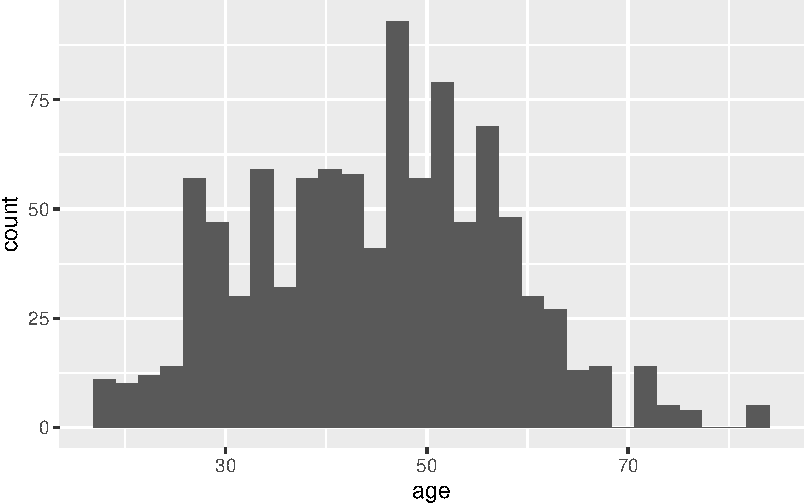
\includegraphics[width=1\textwidth,height=\textheight]{03-intro-data-viz_files/figure-pdf/histogram2-1.pdf}
\end{center}

\subsection{Step 3: Edit the histogram
bins}\label{step-3-edit-the-histogram-bins}

In just two lines of code, we have a histogram! For exploratory data
analysis, this is how \texttt{ggplot2} is such a flexible and quick tool
to get a visual overview of your data.

After running the last code chunk, you might have noticed a message
warning you about the bin width:
\texttt{stat\_bin()\ using\ bins\ =\ 30}. A histogram describes the
frequency of values within your variable. To do so, it must collect the
values into ``bins''. By default - the warning \texttt{ggplot2} gives
you - it uses 30 bins, meaning it tries to plot 30 bars. Depending on
the granularity of your data, you might want more or fewer bins.

You can control this using one of two arguments. First, you can add an
argument called \texttt{binwidth} which sets the bins by how wide you
want the bars on your x-axis scale. For example, we can plot the data
for every 5 years:

\begin{Shaded}
\begin{Highlighting}[]
\CommentTok{\# Plot the variable age from summarydata}
\FunctionTok{ggplot}\NormalTok{(summarydata, }\FunctionTok{aes}\NormalTok{(}\AttributeTok{x =}\NormalTok{ age)) }\SpecialCharTok{+}  \CommentTok{\# Plot age on the x axis}
  \FunctionTok{geom\_histogram}\NormalTok{(}\AttributeTok{binwidth =} \DecValTok{5}\NormalTok{) }\CommentTok{\# collate bins into a 5{-}year span}
\end{Highlighting}
\end{Shaded}

\begin{center}
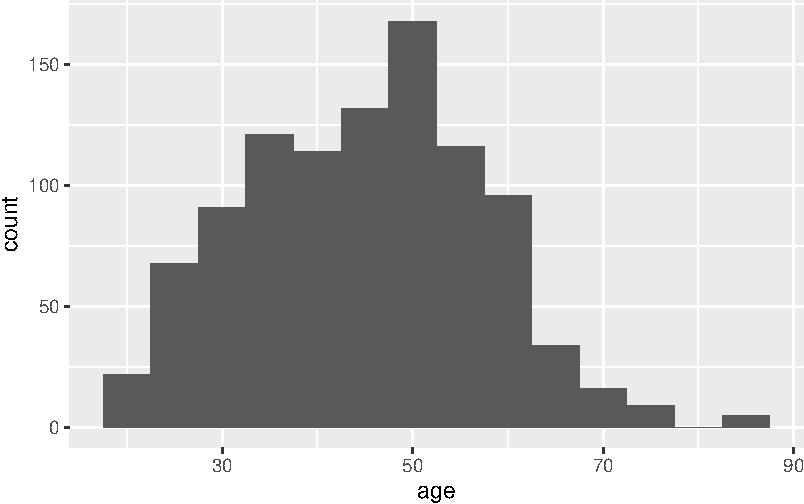
\includegraphics[width=1\textwidth,height=\textheight]{03-intro-data-viz_files/figure-pdf/histogram3a-1.pdf}
\end{center}

Alternatively, you can control precisely how many bars the histograms
uses through the \texttt{bins} argument. For example, we can plot age by
collecting the observations into 10 bars:

\begin{Shaded}
\begin{Highlighting}[]
\CommentTok{\# Plot the variable age from summarydata}
\FunctionTok{ggplot}\NormalTok{(summarydata, }\FunctionTok{aes}\NormalTok{(}\AttributeTok{x =}\NormalTok{ age)) }\SpecialCharTok{+}  \CommentTok{\# Plot age on the x axis}
  \FunctionTok{geom\_histogram}\NormalTok{(}\AttributeTok{bins =} \DecValTok{10}\NormalTok{) }\CommentTok{\# Plot age using 10 bars}
\end{Highlighting}
\end{Shaded}

\begin{center}
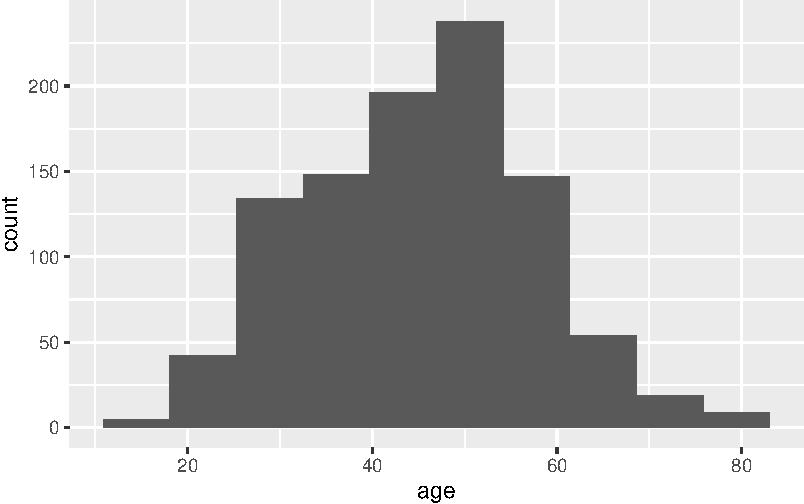
\includegraphics[width=1\textwidth,height=\textheight]{03-intro-data-viz_files/figure-pdf/histogram3b-1.pdf}
\end{center}

\begin{tcolorbox}[enhanced jigsaw, breakable, colframe=quarto-callout-tip-color-frame, arc=.35mm, opacitybacktitle=0.6, titlerule=0mm, colbacktitle=quarto-callout-tip-color!10!white, colback=white, toprule=.15mm, bottomtitle=1mm, toptitle=1mm, title=\textcolor{quarto-callout-tip-color}{\faLightbulb}\hspace{0.5em}{Try this}, bottomrule=.15mm, rightrule=.15mm, leftrule=.75mm, coltitle=black, left=2mm, opacityback=0]

Play around with the \texttt{bin} and \texttt{binwidth} arguments to see
what effect it has on the plot. One of the best ways of learning is
through trial and error to see what effect your changes have on the
result.

\end{tcolorbox}

\subsection{Step 4: Edit the axis
names}\label{step-4-edit-the-axis-names}

By default, the axis names come from the variable names in your data.
When you are making quick plots for yourself, you rarely need to worry
about this. However, as you edit your plot for a report to show other
people, it is normally a good idea to edit the names so they clearly
communicate what they represent.

There are different layers to control the axes depending on the type of
variable you use. Both the x- and y-axis here are continuous numbers, so
we can use the \texttt{scale\_x\_continuous} and
\texttt{scale\_y\_continuous} layers to control them.

There are many options available in \texttt{ggplot2} for controlling the
axes, but you will learn through experience and searching what you need
in different scenarios.

\begin{Shaded}
\begin{Highlighting}[]
\CommentTok{\# Plot the variable age from summarydata}
\FunctionTok{ggplot}\NormalTok{(summarydata, }\FunctionTok{aes}\NormalTok{(}\AttributeTok{x =}\NormalTok{ age)) }\SpecialCharTok{+}  \CommentTok{\# Plot age on the x axis}
  \FunctionTok{geom\_histogram}\NormalTok{(}\AttributeTok{binwidth =} \DecValTok{5}\NormalTok{) }\SpecialCharTok{+} \CommentTok{\# collate bins into a 5{-}year span}
  \FunctionTok{scale\_x\_continuous}\NormalTok{(}\AttributeTok{name =} \StringTok{"Age"}\NormalTok{) }\SpecialCharTok{+}
  \FunctionTok{scale\_y\_continuous}\NormalTok{(}\AttributeTok{name =} \StringTok{"Frequency"}\NormalTok{)}
\end{Highlighting}
\end{Shaded}

\begin{center}
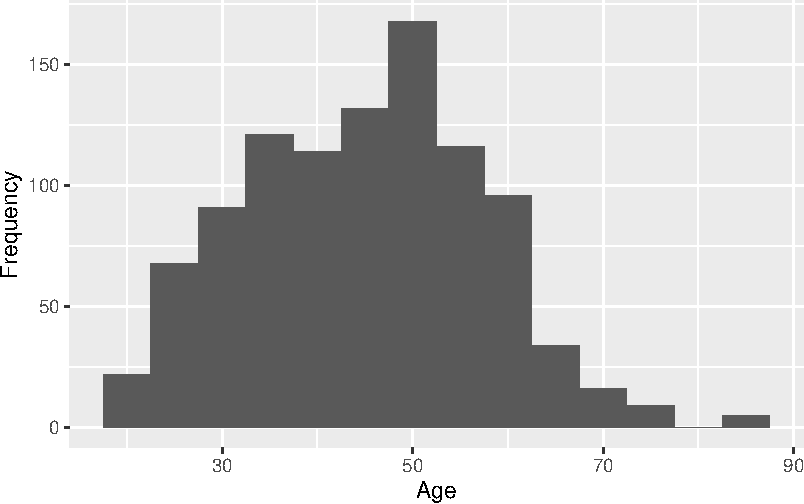
\includegraphics[width=1\textwidth,height=\textheight]{03-intro-data-viz_files/figure-pdf/histogram4-1.pdf}
\end{center}

\subsection{Step 5: Change the plot
theme}\label{step-5-change-the-plot-theme}

So far, we used the default plot theme which has the grey gridlines as a
background. This looks pretty ugly, so we can edit the plot them by
adding a \texttt{theme\_} layer. For example, we can add a
black-and-white theme:

\begin{Shaded}
\begin{Highlighting}[]
\CommentTok{\# Plot the variable age from summarydata}
\FunctionTok{ggplot}\NormalTok{(summarydata, }\FunctionTok{aes}\NormalTok{(}\AttributeTok{x =}\NormalTok{ age)) }\SpecialCharTok{+}  \CommentTok{\# Plot age on the x axis}
  \FunctionTok{geom\_histogram}\NormalTok{(}\AttributeTok{binwidth =} \DecValTok{5}\NormalTok{) }\SpecialCharTok{+} \CommentTok{\# collate bins into a 5{-}year span}
  \FunctionTok{scale\_x\_continuous}\NormalTok{(}\AttributeTok{name =} \StringTok{"Age"}\NormalTok{) }\SpecialCharTok{+}
  \FunctionTok{scale\_y\_continuous}\NormalTok{(}\AttributeTok{name =} \StringTok{"Frequency"}\NormalTok{) }\SpecialCharTok{+} 
  \FunctionTok{theme\_bw}\NormalTok{()}
\end{Highlighting}
\end{Shaded}

\begin{center}
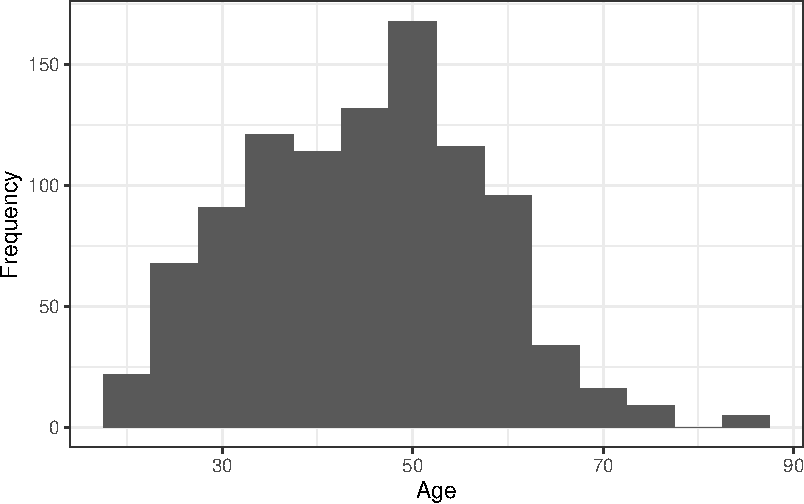
\includegraphics[width=1\textwidth,height=\textheight]{03-intro-data-viz_files/figure-pdf/histogram5-1.pdf}
\end{center}

\begin{tcolorbox}[enhanced jigsaw, breakable, colframe=quarto-callout-tip-color-frame, arc=.35mm, opacitybacktitle=0.6, titlerule=0mm, colbacktitle=quarto-callout-tip-color!10!white, colback=white, toprule=.15mm, bottomtitle=1mm, toptitle=1mm, title=\textcolor{quarto-callout-tip-color}{\faLightbulb}\hspace{0.5em}{Try this}, bottomrule=.15mm, rightrule=.15mm, leftrule=.75mm, coltitle=black, left=2mm, opacityback=0]

There are loads of themes available. As you start typing
\texttt{theme\_}, you should see the full range appear as a drop-down to
autocomplete. Try one or two alternatives such as
\texttt{theme\_classic()} or \texttt{theme\_minimal()} to see how they
look.

\end{tcolorbox}

\subsection{Switch the geom layer}\label{switch-the-geom-layer}

The layer system makes it easy to create new types of plots by adapting
existing recipes. For example, rather than creating a histogram, we can
create a smoothed density plot by calling \texttt{geom\_density()}
rather than \texttt{geom\_histogram()}. Apart from the name of the
y-axis, the rest of the code remains identical to demonstrate how easy
it is to customise your \texttt{ggplot2} layers.

\begin{Shaded}
\begin{Highlighting}[]
\CommentTok{\# Plot the variable age from summarydata}
\FunctionTok{ggplot}\NormalTok{(summarydata, }\FunctionTok{aes}\NormalTok{(}\AttributeTok{x =}\NormalTok{ age)) }\SpecialCharTok{+}  \CommentTok{\# Plot age on the x axis}
  \FunctionTok{geom\_density}\NormalTok{() }\SpecialCharTok{+} \CommentTok{\# summarise age as a smoothed density plot}
  \FunctionTok{scale\_x\_continuous}\NormalTok{(}\AttributeTok{name =} \StringTok{"Age"}\NormalTok{) }\SpecialCharTok{+}
  \FunctionTok{scale\_y\_continuous}\NormalTok{(}\AttributeTok{name =} \StringTok{"Density"}\NormalTok{) }\SpecialCharTok{+} 
  \FunctionTok{theme\_bw}\NormalTok{()}
\end{Highlighting}
\end{Shaded}

\begin{center}
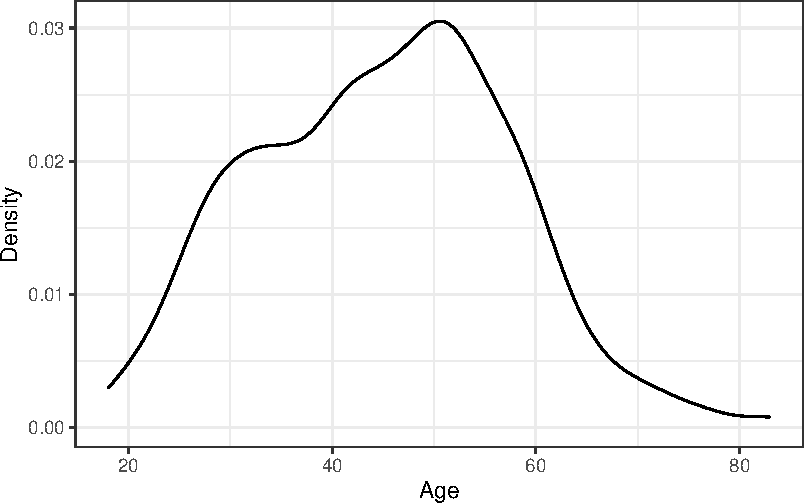
\includegraphics[width=1\textwidth,height=\textheight]{03-intro-data-viz_files/figure-pdf/density-rt-1.pdf}
\end{center}

\subsection{Activity 5 - Apply your plotting skills to a new
variable}\label{activity-5---apply-your-plotting-skills-to-a-new-variable}

Before we move on to barplots, an important learning step is being able
to apply or transfer what you learnt in one scenario to something new.

In the data set, there is a variable for The Authentic Happiness
Inventory (AHI): \texttt{ahiTotal}. Plot the new variable and try to
recreate the customisation layers before checking the solution below. It
might take some trial-and-error to get some features right, so do not
worry if it does not immediately look the same.

\begin{center}
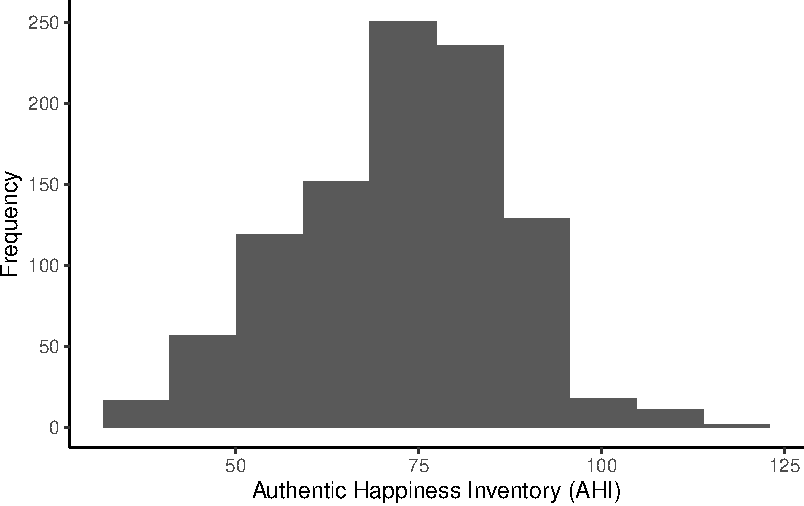
\includegraphics[width=1\textwidth,height=\textheight]{03-intro-data-viz_files/figure-pdf/unnamed-chunk-6-1.pdf}
\end{center}

\begin{tcolorbox}[enhanced jigsaw, breakable, colframe=quarto-callout-tip-color-frame, arc=.35mm, opacitybacktitle=0.6, titlerule=0mm, colbacktitle=quarto-callout-tip-color!10!white, colback=white, toprule=.15mm, bottomtitle=1mm, toptitle=1mm, title=\textcolor{quarto-callout-tip-color}{\faLightbulb}\hspace{0.5em}{Show me the solution code}, bottomrule=.15mm, rightrule=.15mm, leftrule=.75mm, coltitle=black, left=2mm, opacityback=0]

To recreate the plot, this is the code:

\begin{Shaded}
\begin{Highlighting}[]
\CommentTok{\# Plot the variable ahi total from summarydata}
\FunctionTok{ggplot}\NormalTok{(summarydata, }\FunctionTok{aes}\NormalTok{(}\AttributeTok{x =}\NormalTok{ ahiTotal)) }\SpecialCharTok{+}  \CommentTok{\# Plot ahi total on the x axis}
  \FunctionTok{geom\_histogram}\NormalTok{(}\AttributeTok{bins =} \DecValTok{10}\NormalTok{) }\SpecialCharTok{+} 
  \FunctionTok{scale\_x\_continuous}\NormalTok{(}\AttributeTok{name =} \StringTok{"Authentic Happiness Inventory (AHI)"}\NormalTok{) }\SpecialCharTok{+}
  \FunctionTok{scale\_y\_continuous}\NormalTok{(}\AttributeTok{name =} \StringTok{"Frequency"}\NormalTok{) }\SpecialCharTok{+} 
  \FunctionTok{theme\_classic}\NormalTok{()}
\end{Highlighting}
\end{Shaded}

We were a little sneaky with using the classic theme to get you
exploring.

\end{tcolorbox}

\section{Barplots}\label{barplots}

In the next section, we are going to cover making barplots - potentially
the most common type of visualisation you will see in published
research. A barplot shows counts of categorical data, or factors, where
the height of each bar represents the count of that particular variable.

You will see people use them to represent continuous outcomes, such as
showing the mean on the y-axis, but there is good reason to never use
bar plots to communicate continuous data we will cover in the course
materials (see Weissgerber et al., 2019 if you are interested). We will
cover more advanced plots for continuous data in
\hyperref[07-more-viz]{Chapter 7 - Building your data visualisation
skills}.

\subsection{Activity 6 - Convert to factors}\label{introviz-a2}

Earlier, we highlighted that all the variables were processed as
numbers. This was fine for most of the variables, but \texttt{sex},
\texttt{educ}, and \texttt{income} should be categories or what we call
\textbf{factors}.

To get around this, we need to convert these variables into factors.
This is relates to data wrangling, so this is one final time we would
like you to copy and run code, before we fully explain how to write this
kind of code independently in the next chapter.

Copy and run the following code in your R Markdown document, at least
below where you read and wrangled the data:

\begin{Shaded}
\begin{Highlighting}[]
\CommentTok{\# Overwrite summary data }
\NormalTok{summarydata }\OtherTok{\textless{}{-}} \FunctionTok{mutate}\NormalTok{(summarydata, }\CommentTok{\# mutate to change columns }
         \AttributeTok{sex =} \FunctionTok{as.factor}\NormalTok{(sex), }\CommentTok{\# save sex as a factor}
         \AttributeTok{educ =} \FunctionTok{as.factor}\NormalTok{(educ),}
         \AttributeTok{income =} \FunctionTok{as.factor}\NormalTok{(income))}
\end{Highlighting}
\end{Shaded}

You can interpret this code as ``overwrite \texttt{summarydata} and
transform three columns (\texttt{sex}, \texttt{educ}, and
\texttt{income}) into the same values but now considered factors and not
doubles''.

\begin{tcolorbox}[enhanced jigsaw, breakable, colframe=quarto-callout-important-color-frame, arc=.35mm, opacitybacktitle=0.6, titlerule=0mm, colbacktitle=quarto-callout-important-color!10!white, colback=white, toprule=.15mm, bottomtitle=1mm, toptitle=1mm, title=\textcolor{quarto-callout-important-color}{\faExclamation}\hspace{0.5em}{Error mode}, bottomrule=.15mm, rightrule=.15mm, leftrule=.75mm, coltitle=black, left=2mm, opacityback=0]

If you do not do convert numbers to factors when they should represent
distinct categories, you can get some weird looking figures. Instead of
treating the numbers as categories, it will try and plot the full range
of numerical values. If you notice this, just go back and convert your
variables to factors (which we will break down in the next chapter).

\end{tcolorbox}

\subsection{Activity 7 - Create a bar plot}\label{introviz-a3}

Now you are familiar with the layering system, we will jump straight
into creating the barplot. As before, type and run the code in each
step, making notes to yourself either in the R Markdown document outside
the code chunks, or using code comments.

\begin{Shaded}
\begin{Highlighting}[]
\CommentTok{\# Plot the variable sex from summarydata}
\FunctionTok{ggplot}\NormalTok{(summarydata, }\FunctionTok{aes}\NormalTok{(}\AttributeTok{x =}\NormalTok{ sex)) }\SpecialCharTok{+} 
  \FunctionTok{geom\_bar}\NormalTok{()}
\end{Highlighting}
\end{Shaded}

\begin{center}
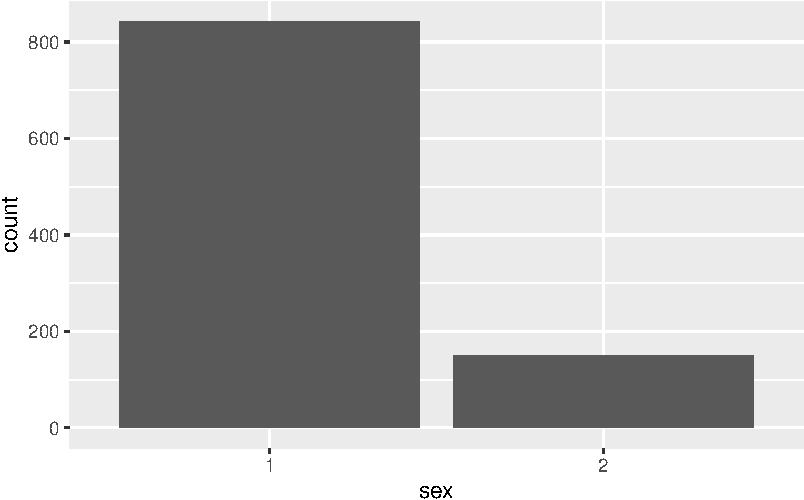
\includegraphics[width=1\textwidth,height=\textheight]{03-intro-data-viz_files/figure-pdf/barplot1-1.pdf}
\end{center}

Compared to the histogram plot, the only difference here is using the
\texttt{geom\_bar()} as the layer instead. Rather than plot the
frequency of your variable in bins, we plot the frequency of each unique
category.

We can see 1s are way more frequent than 2s, but for this to make sense
to you and your reader, we need to edit the axis labels.

\subsection{Activity 8 - Edit the axis
labels}\label{activity-8---edit-the-axis-labels}

In the histogram section, we demonstrated how to edit the axis labels.
We used \texttt{scale\_y\_continuous} and \texttt{scale\_x\_continuous}
as we had two continuous variables for the x-axis range and the y-axis
frequency. This time, we need a slightly different layer since the
x-axis now represents distinct groups: \texttt{scale\_x\_discrete}.

Type and run the following code:

\begin{Shaded}
\begin{Highlighting}[]
\CommentTok{\# Plot the variable sex from summarydata}
\FunctionTok{ggplot}\NormalTok{(summarydata, }\FunctionTok{aes}\NormalTok{(}\AttributeTok{x =}\NormalTok{ sex)) }\SpecialCharTok{+} 
  \FunctionTok{geom\_bar}\NormalTok{() }\SpecialCharTok{+} 
  \FunctionTok{scale\_x\_discrete}\NormalTok{(}\AttributeTok{name =} \StringTok{"Participant Sex"}\NormalTok{, }
                   \AttributeTok{labels =} \FunctionTok{c}\NormalTok{(}\StringTok{"Female"}\NormalTok{, }\CommentTok{\# 1 = Female}
                              \StringTok{"Male"}\NormalTok{)) }\SpecialCharTok{+} \CommentTok{\# 2 = Male}
  \FunctionTok{scale\_y\_continuous}\NormalTok{(}\AttributeTok{name =} \StringTok{"Number of Participants"}\NormalTok{)}
\end{Highlighting}
\end{Shaded}

\begin{center}
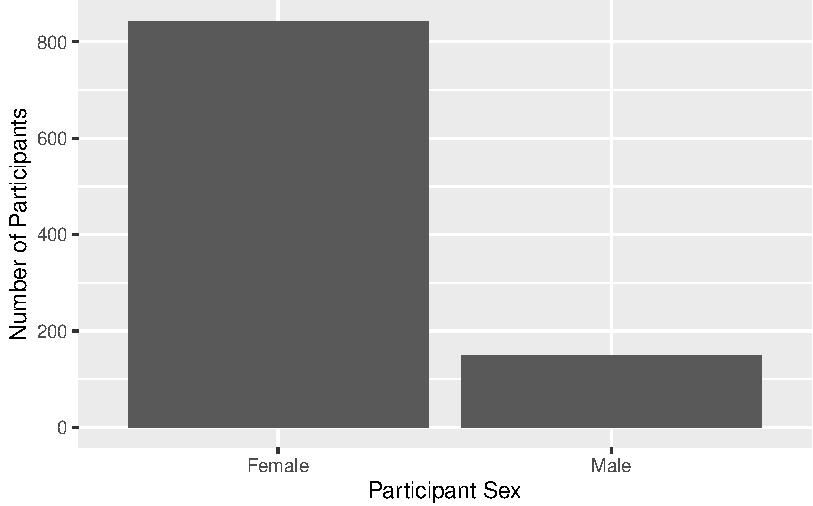
\includegraphics[width=1\textwidth,height=\textheight]{03-intro-data-viz_files/figure-pdf/unnamed-chunk-8-1.pdf}
\end{center}

Within \texttt{scale\_x\_discrete}, we have a new argument called
``labels''. This is where we can edit the labels for each category.
Instead of 1 and 2, we labelled the x-axis clearer as ``Female'' and
``Male'', making it easier to understand there are way more female
participants compared to male.

\begin{tcolorbox}[enhanced jigsaw, breakable, colframe=quarto-callout-note-color-frame, arc=.35mm, opacitybacktitle=0.6, titlerule=0mm, colbacktitle=quarto-callout-note-color!10!white, colback=white, toprule=.15mm, bottomtitle=1mm, toptitle=1mm, title=\textcolor{quarto-callout-note-color}{\faInfo}\hspace{0.5em}{What does \texttt{c()} mean in labels?}, bottomrule=.15mm, rightrule=.15mm, leftrule=.75mm, coltitle=black, left=2mm, opacityback=0]

When we specified the labels, you might have noticed the
\texttt{c("Female",\ "Male")} format. \texttt{c()} stands for
concatenate and you will see it a lot in R. When we give a value to a
function argument, we must provide one ``value''. However, in scenarios
like this, we want to apply multiple values since we have several
categories.

We can do this by adding all of our categories within \texttt{c()},
separated by a comma between each category.

\end{tcolorbox}

\begin{tcolorbox}[enhanced jigsaw, breakable, colframe=quarto-callout-important-color-frame, arc=.35mm, opacitybacktitle=0.6, titlerule=0mm, colbacktitle=quarto-callout-important-color!10!white, colback=white, toprule=.15mm, bottomtitle=1mm, toptitle=1mm, title=\textcolor{quarto-callout-important-color}{\faExclamation}\hspace{0.5em}{Error mode}, bottomrule=.15mm, rightrule=.15mm, leftrule=.75mm, coltitle=black, left=2mm, opacityback=0]

When you edit ``labels'', it is crucial the values you give it are in
the right order. There would be nothing stopping us from writing
\texttt{c("Male",\ "Female")} and R will gladly listen to you and add
those labels. However, that would be inaccurate as 1s mean Female and 2s
mean Male. We are only editing the labels and not the underlying values
in the data.

These errors are the most sneaky as it will not cause an error to fix,
but they are still incorrect.

\end{tcolorbox}

\subsection{Activity 9 - Apply your plotting skills to a new
variable}\label{activity-9---apply-your-plotting-skills-to-a-new-variable}

An important learning step is being able to apply or transfer what you
learnt in one scenario to something new.

In the data set, there is a variable for the level of education:
\texttt{educ}. Plot the new variable and try to recreate the
customisation layers before checking the solution below.

\begin{center}
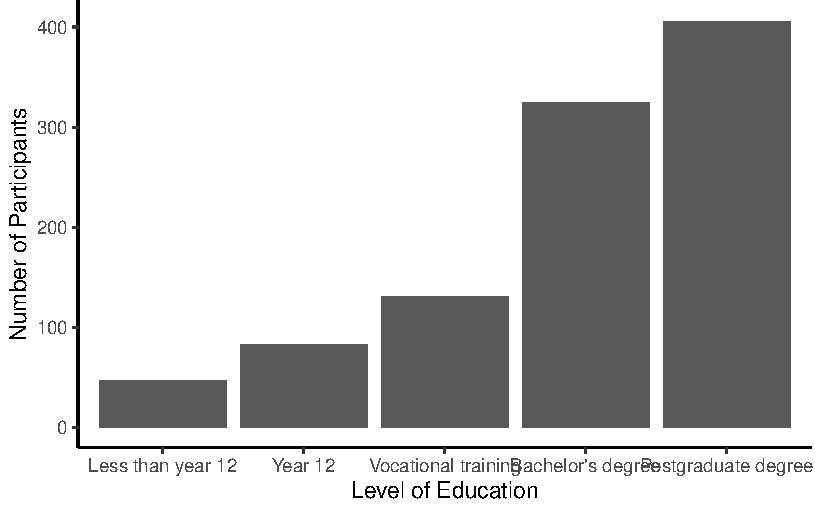
\includegraphics[width=1\textwidth,height=\textheight]{03-intro-data-viz_files/figure-pdf/unnamed-chunk-9-1.pdf}
\end{center}

\begin{tcolorbox}[enhanced jigsaw, breakable, colframe=quarto-callout-tip-color-frame, arc=.35mm, opacitybacktitle=0.6, titlerule=0mm, colbacktitle=quarto-callout-tip-color!10!white, colback=white, toprule=.15mm, bottomtitle=1mm, toptitle=1mm, title=\textcolor{quarto-callout-tip-color}{\faLightbulb}\hspace{0.5em}{Show me the solution code}, bottomrule=.15mm, rightrule=.15mm, leftrule=.75mm, coltitle=black, left=2mm, opacityback=0]

To recreate the plot, this is the code:

\begin{Shaded}
\begin{Highlighting}[]
\CommentTok{\# Plot the variable educ from summarydata}
\FunctionTok{ggplot}\NormalTok{(summarydata, }\FunctionTok{aes}\NormalTok{(}\AttributeTok{x =}\NormalTok{ educ)) }\SpecialCharTok{+} 
  \FunctionTok{geom\_bar}\NormalTok{() }\SpecialCharTok{+} 
  \FunctionTok{theme\_classic}\NormalTok{() }\SpecialCharTok{+} 
  \FunctionTok{scale\_x\_discrete}\NormalTok{(}\AttributeTok{name =} \StringTok{"Level of Education"}\NormalTok{, }
                   \AttributeTok{labels =} \FunctionTok{c}\NormalTok{(}\StringTok{"Less than year 12"}\NormalTok{, }\CommentTok{\# 1}
                              \StringTok{"Year 12"}\NormalTok{, }\CommentTok{\# 2 }
                              \StringTok{"Vocational training"}\NormalTok{, }\CommentTok{\# 3}
                              \StringTok{"Bachelor\textquotesingle{}s degree"}\NormalTok{, }\CommentTok{\# 4}
                              \StringTok{"Postgraduate degree"}\NormalTok{)) }\SpecialCharTok{+} \CommentTok{\# 5 }
  \FunctionTok{scale\_y\_continuous}\NormalTok{(}\AttributeTok{name =} \StringTok{"Number of Participants"}\NormalTok{)}
\end{Highlighting}
\end{Shaded}

\end{tcolorbox}

\section{Saving your Figures}\label{saving-your-figures}

The final step today will be to demonstrate how to save plots you create
in \texttt{ggplot2}. It is so useful to be able to save a copy of your
plots as an image file so that you can use them in a presentation or
report. One approach we can use is the function \texttt{ggsave()}.

\subsection{Activity 10 - Saving your last plot}\label{introviz-a6}

There are two ways you can use \texttt{ggsave()}. If you do not tell
\texttt{ggsave()} which plot you want to save, by default it will save
\textbf{the last plot you created}.

To demonstrate this, let us run the code again from Activity 8 to
produce the final version of our barplot. You do not need to write the
code again if you already have it available in a code chunk, but make
sure you run the code:

\begin{Shaded}
\begin{Highlighting}[]
\CommentTok{\# Plot the variable sex from summarydata}
\FunctionTok{ggplot}\NormalTok{(summarydata, }\FunctionTok{aes}\NormalTok{(}\AttributeTok{x =}\NormalTok{ sex)) }\SpecialCharTok{+} 
  \FunctionTok{geom\_bar}\NormalTok{() }\SpecialCharTok{+} 
  \FunctionTok{scale\_x\_discrete}\NormalTok{(}\AttributeTok{name =} \StringTok{"Participant Sex"}\NormalTok{, }
                   \AttributeTok{labels =} \FunctionTok{c}\NormalTok{(}\StringTok{"Female"}\NormalTok{, }\CommentTok{\# 1 = Female}
                              \StringTok{"Male"}\NormalTok{)) }\SpecialCharTok{+} \CommentTok{\# 2 = Male}
  \FunctionTok{scale\_y\_continuous}\NormalTok{(}\AttributeTok{name =} \StringTok{"Number of Participants"}\NormalTok{)}
\end{Highlighting}
\end{Shaded}

Now that we have the plot we want to save as our last produced plot, all
that \texttt{ggsave()} requires is for you to tell it the file path /
name that it should save the plot to and the type of image file you want
to create. The example below uses .png but you could also use .jpeg or
another image type.

Type and run the following code into a new code chunk and then check
your \texttt{figures} folder. If you have performed this correctly, then
you should see the saved image. This is why we include a
\texttt{figures} folder as part of the chapter structure, so you know
exactly where your figures will be if you want to find them again.

\begin{Shaded}
\begin{Highlighting}[]
\FunctionTok{ggsave}\NormalTok{(}\StringTok{"figures/participant\_sex\_barplot.png"}\NormalTok{)}
\end{Highlighting}
\end{Shaded}

The image tends to save at a default size, or the size that the image is
displayed in your viewer, but you can change this manually if you think
that the dimensions of the plot are not correct or if you need a
particular size or file type. Sometimes the dimensions look a little off
when you save them, so you might need to play around with the size.

Type and run the following code to overwrite the image file with new
dimensions. Try different dimensions and units to see the difference.
You might want to create \texttt{participant\_sex\_barplot-v1.png},
\texttt{participant\_sex\_barplot-v2.png} etc. and compare them.

One final tip, by default, the plot has a transparent background which
you do not notice on a white document, but looks odd on anything else.
So, you can set a specific background colour through the argument
\texttt{bg}.

\begin{Shaded}
\begin{Highlighting}[]
 \FunctionTok{ggsave}\NormalTok{(}\StringTok{"figures/participant\_sex\_barplot.png"}\NormalTok{, }
        \AttributeTok{width =} \DecValTok{10}\NormalTok{, }\CommentTok{\# 10 inches wide}
        \AttributeTok{height =} \DecValTok{8}\NormalTok{, }\CommentTok{\# 8 inches high}
        \AttributeTok{units =} \StringTok{"in"}\NormalTok{, }
        \AttributeTok{bg =} \StringTok{"white"}\NormalTok{) }\CommentTok{\# Make sure the background is white}
\end{Highlighting}
\end{Shaded}

Remember, you can use \texttt{?ggsave()} in the console window to bring
up the help file for this function if you want to look at what other
arguments are available.

\subsection{Saving a specific plot}\label{saving-a-specific-plot}

Alternatively, the second way of using \texttt{ggsave()} is to save your
plot as an object, and then tell it which object you want to save.

Type and run the code below and then check your folder for the image
file. Resize the plot if you think it needs it.

\begin{tcolorbox}[enhanced jigsaw, breakable, colframe=quarto-callout-warning-color-frame, arc=.35mm, opacitybacktitle=0.6, titlerule=0mm, colbacktitle=quarto-callout-warning-color!10!white, colback=white, toprule=.15mm, bottomtitle=1mm, toptitle=1mm, title=\textcolor{quarto-callout-warning-color}{\faExclamationTriangle}\hspace{0.5em}{Warning}, bottomrule=.15mm, rightrule=.15mm, leftrule=.75mm, coltitle=black, left=2mm, opacityback=0]

We do not add on \texttt{ggsave()} as a plot layer. Instead it is a
separate line of code and we tell it which object to save. So, do not
add \texttt{+\ ggsave()} as a layer to your plot.

\end{tcolorbox}

\begin{Shaded}
\begin{Highlighting}[]
\NormalTok{sex\_barplot }\OtherTok{\textless{}{-}} \FunctionTok{ggplot}\NormalTok{(summarydata, }\FunctionTok{aes}\NormalTok{(}\AttributeTok{x =}\NormalTok{ sex)) }\SpecialCharTok{+}
  \FunctionTok{geom\_bar}\NormalTok{() }\SpecialCharTok{+}
  \FunctionTok{scale\_x\_discrete}\NormalTok{(}\AttributeTok{name =} \StringTok{"Participant Sex"}\NormalTok{,}
                   \AttributeTok{labels =} \FunctionTok{c}\NormalTok{(}\StringTok{"Female"}\NormalTok{, }\CommentTok{\# 1 = Female}
                              \StringTok{"Male"}\NormalTok{)) }\SpecialCharTok{+} \CommentTok{\# 2 = Male}
  \FunctionTok{scale\_y\_continuous}\NormalTok{(}\AttributeTok{name =} \StringTok{"Number of Participants"}\NormalTok{)}


\FunctionTok{ggsave}\NormalTok{(}\StringTok{"figures/participant{-}sex{-}barplot.png"}\NormalTok{, }
       \AttributeTok{plot =}\NormalTok{ sex\_barplot)}
\end{Highlighting}
\end{Shaded}

Note that when you save a plot to an object, you will not see the plot
displayed anywhere. To get the figure to display, you need to type the
object name in the console (i.e., \texttt{sex\_barplot}). The benefit of
saving figures this way is that if you are making several plots, you
cannot accidentally save the wrong one because you are explicitly
specifying which plot to save rather than just saving the last one.

\section{Test Yourself}\label{test-yourself-2}

To end the chapter, we have some knowledge check questions to test your
understanding of the concepts we covered in the chapter. We then have
some error mode tasks to see if you can find the solution to some common
errors in the concepts we covered in this chapter.

\subsection{Knowledge check}\label{knowledge-check-2}

\textbf{Question 1.} Which of these is the appropriate order of
functions to create a barplot?

\begin{itemize}
\tightlist
\item
  \begin{enumerate}
  \def\labelenumi{(\Alph{enumi})}
  \tightlist
  \item
    geom\_bar() + ggplot()\\
  \end{enumerate}
\item
  \begin{enumerate}
  \def\labelenumi{(\Alph{enumi})}
  \setcounter{enumi}{1}
  \tightlist
  \item
    ggplot() + geom\_bar()\\
  \end{enumerate}
\item
  \begin{enumerate}
  \def\labelenumi{(\Alph{enumi})}
  \setcounter{enumi}{2}
  \tightlist
  \item
    geom\_plot() + geom\_boxplot()\\
  \end{enumerate}
\item
  \begin{enumerate}
  \def\labelenumi{(\Alph{enumi})}
  \setcounter{enumi}{3}
  \tightlist
  \item
    ggplot() \%\textgreater\% geom\_bar()
  \end{enumerate}
\end{itemize}

\textbf{Question 2.} Why would this line of code not create a barplot,
assuming you already loaded all data and libraries and you spelt the
data and column names correctly?

\begin{Shaded}
\begin{Highlighting}[]
\FunctionTok{ggplot}\NormalTok{(summarydata, }\FunctionTok{aes}\NormalTok{(}\AttributeTok{x =}\NormalTok{ sex)) }\SpecialCharTok{+}
  \FunctionTok{geom\_barplot}\NormalTok{()}
\end{Highlighting}
\end{Shaded}

\begin{itemize}
\tightlist
\item
  \begin{enumerate}
  \def\labelenumi{(\Alph{enumi})}
  \tightlist
  \item
    because this would create a histogram\\
  \end{enumerate}
\item
  \begin{enumerate}
  \def\labelenumi{(\Alph{enumi})}
  \setcounter{enumi}{1}
  \tightlist
  \item
    because you have piped the barplot and not added it\\
  \end{enumerate}
\item
  \begin{enumerate}
  \def\labelenumi{(\Alph{enumi})}
  \setcounter{enumi}{2}
  \tightlist
  \item
    because you have not included a y axis\\
  \end{enumerate}
\item
  \begin{enumerate}
  \def\labelenumi{(\Alph{enumi})}
  \setcounter{enumi}{3}
  \tightlist
  \item
    because there is no geom\_barplot() and it should be geom\_bar()
  \end{enumerate}
\end{itemize}

\textbf{Question 3.} If I wanted precisely 5 bars in my histogram, what
argument would I use?

\begin{itemize}
\tightlist
\item
  \begin{enumerate}
  \def\labelenumi{(\Alph{enumi})}
  \tightlist
  \item
    ggplot() + geom\_histogram(binwidth = 5)\\
  \end{enumerate}
\item
  \begin{enumerate}
  \def\labelenumi{(\Alph{enumi})}
  \setcounter{enumi}{1}
  \tightlist
  \item
    ggplot() + geom\_histogram()\\
  \end{enumerate}
\item
  \begin{enumerate}
  \def\labelenumi{(\Alph{enumi})}
  \setcounter{enumi}{2}
  \tightlist
  \item
    ggplot() + geom\_histogram(bins = 5)\\
  \end{enumerate}
\item
  \begin{enumerate}
  \def\labelenumi{(\Alph{enumi})}
  \setcounter{enumi}{3}
  \tightlist
  \item
    ggplot() + geom\_histogram(bars = 5)
  \end{enumerate}
\end{itemize}

\begin{tcolorbox}[enhanced jigsaw, breakable, colframe=quarto-callout-caution-color-frame, arc=.35mm, opacitybacktitle=0.6, titlerule=0mm, colbacktitle=quarto-callout-caution-color!10!white, colback=white, toprule=.15mm, bottomtitle=1mm, toptitle=1mm, title=\textcolor{quarto-callout-caution-color}{\faFire}\hspace{0.5em}{Explain this answer}, bottomrule=.15mm, rightrule=.15mm, leftrule=.75mm, coltitle=black, left=2mm, opacityback=0]

\begin{itemize}
\item
  \texttt{ggplot()\ +\ geom\_histogram(bins\ =\ 5)}. This is the
  \textbf{correct} answer as you are asking ggplot2 to give you the plot
  organised into 5 bins.
\item
  \texttt{ggplot()\ +\ geom\_histogram(bars\ =\ 5)}. This is incorrect
  as you bars is not the right argument name. You want 5 bars, but the
  argument is bins.
\item
  \texttt{ggplot()\ +\ geom\_histogram(binwidth\ =\ 5)}. This is
  incorrect as binwidth controls the x-axis range to include per bar,
  rather than the number of bars.
\item
  \texttt{ggplot()\ +\ geom\_histogram()}. This is incorrect as you did
  not control the number of bins, so it will default to 30.
\end{itemize}

\end{tcolorbox}

\subsection{Error mode}\label{error-mode-8}

The following questions are designed to introduce you to making and
fixing errors. For this topic, we focus on reading data and using
ggplot2. Remember to keep a note of what kind of error messages you
receive and how you fixed them, so you have a bank of solutions when you
tackle errors independently.

Create and save a new R Markdown file for these activities by following
the instructions in Chapter 2. You should have a blank R Markdown file
below line 10. Below, we have several variations of a code chunk and
inline code errors. Copy and paste them into your R Markdown file, click
knit, and look at the error message you receive. See if you can fix the
error and get it working before checking the answer.

\textbf{Question 4}. Copy the following code chunk into your R Markdown
file and press knit. You should receive an error like
\texttt{Error\ in\ read\_csv():\ !\ could\ not\ find\ function\ "read\_csv"}.

\begin{Shaded}
\begin{Highlighting}[]
\InformationTok{\textasciigrave{}\textasciigrave{}\textasciigrave{}\{r\}}
\InformationTok{pinfo \textless{}{-} read\_csv("data/participant{-}info.csv")}
\InformationTok{\textasciigrave{}\textasciigrave{}\textasciigrave{}}
\end{Highlighting}
\end{Shaded}

\begin{tcolorbox}[enhanced jigsaw, breakable, colframe=quarto-callout-caution-color-frame, arc=.35mm, opacitybacktitle=0.6, titlerule=0mm, colbacktitle=quarto-callout-caution-color!10!white, colback=white, toprule=.15mm, bottomtitle=1mm, toptitle=1mm, title=\textcolor{quarto-callout-caution-color}{\faFire}\hspace{0.5em}{Explain the solution}, bottomrule=.15mm, rightrule=.15mm, leftrule=.75mm, coltitle=black, left=2mm, opacityback=0]

If you only added this code chunk in, you have not loaded tidyverse yet.
Remember R Markdown knits from start to finish in a fresh session, so it
will not work even if you have loaded already tidyverse outside the R
Markdown document. So, you would need to add \texttt{library(tidyverse)}
first.

\end{tcolorbox}

\textbf{Question 5}. Copy the following code chunk into your R Markdown
file and press knit. You should receive an error like
\texttt{!\ participant-info.csv\ does\ not\ exist\ in\ current\ working\ directory}.

\begin{Shaded}
\begin{Highlighting}[]
\InformationTok{\textasciigrave{}\textasciigrave{}\textasciigrave{}\{r\}}
\InformationTok{library(tidyverse)}

\InformationTok{pinfo \textless{}{-} read\_csv("participant{-}info.csv")}
\InformationTok{\textasciigrave{}\textasciigrave{}\textasciigrave{}}
\end{Highlighting}
\end{Shaded}

\begin{tcolorbox}[enhanced jigsaw, breakable, colframe=quarto-callout-caution-color-frame, arc=.35mm, opacitybacktitle=0.6, titlerule=0mm, colbacktitle=quarto-callout-caution-color!10!white, colback=white, toprule=.15mm, bottomtitle=1mm, toptitle=1mm, title=\textcolor{quarto-callout-caution-color}{\faFire}\hspace{0.5em}{Explain the solution}, bottomrule=.15mm, rightrule=.15mm, leftrule=.75mm, coltitle=black, left=2mm, opacityback=0]

You had tidyverse loaded this time, but it is not pointing to the right
folder. Your working directory should be the main chapter folder, where
\texttt{participant-info.csv} does not exist. You will need to edit it
to \texttt{data/participant-info.csv} to work.

\end{tcolorbox}

\textbf{Question 6}. Copy the following code chunk into your R Markdown
file and press knit. You should receive a long error where the problem
is buried in the first five lines:

\begin{quote}
\texttt{Error\ in\ geom\_histogram()}
\end{quote}

\begin{quote}
\texttt{!\ Problem\ while\ computing\ stat.}
\end{quote}

\begin{quote}
\texttt{i\ Error\ occurred\ in\ the\ 1st\ layer.}
\end{quote}

\begin{quote}
\texttt{Caused\ by\ error\ in\ setup\_params():}
\end{quote}

\begin{quote}
\texttt{!\ stat\_bin()\ requires\ an\ x\ or\ y\ aesthetic.}
\end{quote}

\begin{Shaded}
\begin{Highlighting}[]
\InformationTok{\textasciigrave{}\textasciigrave{}\textasciigrave{}\{r\}}
\InformationTok{library(tidyverse)}

\InformationTok{pinfo \textless{}{-} read\_csv("data/participant{-}info.csv")}

\InformationTok{\# Plot the variable age from pinfo}
\InformationTok{ggplot(pinfo, x = age) +   \# Plot age on the x axis}
\InformationTok{  geom\_histogram()}
\InformationTok{\textasciigrave{}\textasciigrave{}\textasciigrave{}}
\end{Highlighting}
\end{Shaded}

\begin{tcolorbox}[enhanced jigsaw, breakable, colframe=quarto-callout-caution-color-frame, arc=.35mm, opacitybacktitle=0.6, titlerule=0mm, colbacktitle=quarto-callout-caution-color!10!white, colback=white, toprule=.15mm, bottomtitle=1mm, toptitle=1mm, title=\textcolor{quarto-callout-caution-color}{\faFire}\hspace{0.5em}{Explain the solution}, bottomrule=.15mm, rightrule=.15mm, leftrule=.75mm, coltitle=black, left=2mm, opacityback=0]

This is potentially a sneaky one where we missed the \texttt{aes()}
argument and it is only line 5 of the error which gives it away:
\texttt{!\ stat\_bin()\ requires\ an\ x\ or\ y\ aesthetic}. The first
ggplot2 layer has two key components: the data object you want to use,
and the aesthetics to set. You need to add ``aes()'' around where you
specify the x-axis: \texttt{ggplot(pinfo,\ aes(x\ =\ age))}.

\end{tcolorbox}

\textbf{Question 7}. Copy the following code chunk into your R Markdown
file and press knit. This\ldots works, but does not look quite right?

\begin{Shaded}
\begin{Highlighting}[]
\InformationTok{\textasciigrave{}\textasciigrave{}\textasciigrave{}\{r\}}
\InformationTok{library(tidyverse)}

\InformationTok{pinfo \textless{}{-} read\_csv("data/participant{-}info.csv")}

\InformationTok{\# Plot the variable age from pinfo}
\InformationTok{ggplot(pinfo, aes(x = age)) \# Plot age on the x axis}
\InformationTok{  geom\_histogram()}
\InformationTok{\textasciigrave{}\textasciigrave{}\textasciigrave{}}
\end{Highlighting}
\end{Shaded}

\begin{tcolorbox}[enhanced jigsaw, breakable, colframe=quarto-callout-caution-color-frame, arc=.35mm, opacitybacktitle=0.6, titlerule=0mm, colbacktitle=quarto-callout-caution-color!10!white, colback=white, toprule=.15mm, bottomtitle=1mm, toptitle=1mm, title=\textcolor{quarto-callout-caution-color}{\faFire}\hspace{0.5em}{Explain the solution}, bottomrule=.15mm, rightrule=.15mm, leftrule=.75mm, coltitle=black, left=2mm, opacityback=0]

There is a missing \texttt{+} between the two ggplot2 layers. The code
should be:

\begin{Shaded}
\begin{Highlighting}[]
\CommentTok{\# Plot the variable age from pinfo}
\FunctionTok{ggplot}\NormalTok{(pinfo, }\FunctionTok{aes}\NormalTok{(}\AttributeTok{x =}\NormalTok{ age)) }\SpecialCharTok{+}  \CommentTok{\# Plot age on the x axis}
  \FunctionTok{geom\_histogram}\NormalTok{()}
\end{Highlighting}
\end{Shaded}

At the moment, it runs the first layer to create an empty plot, then
prints the information contained within geom\_histogram.

\end{tcolorbox}

\textbf{Question 8}. Copy the following code chunk into your R Markdown
file and press knit. You should receive a long error again with lines
5-7 key:

\begin{quote}
\texttt{!\ stat\_bin()\ requires\ a\ continuous\ x\ aesthetic.}
\end{quote}

\begin{quote}
\texttt{x\ the\ x\ aesthetic\ is\ discrete.}
\end{quote}

\begin{quote}
\texttt{i\ Perhaps\ you\ want\ stat="count"?}
\end{quote}

\begin{Shaded}
\begin{Highlighting}[]
\InformationTok{\textasciigrave{}\textasciigrave{}\textasciigrave{}\{r\}}
\InformationTok{library(tidyverse)}

\InformationTok{pinfo \textless{}{-} read\_csv("data/participant{-}info.csv")}

\InformationTok{\# Plot the variable age from pinfo}
\InformationTok{ggplot(pinfo, aes(x = age)) +   \# Plot age on the x axis}
\InformationTok{  geom\_histogram() + }
\InformationTok{  scale\_x\_discrete(name = "Participant Age")}
\InformationTok{\textasciigrave{}\textasciigrave{}\textasciigrave{}}
\end{Highlighting}
\end{Shaded}

\begin{tcolorbox}[enhanced jigsaw, breakable, colframe=quarto-callout-caution-color-frame, arc=.35mm, opacitybacktitle=0.6, titlerule=0mm, colbacktitle=quarto-callout-caution-color!10!white, colback=white, toprule=.15mm, bottomtitle=1mm, toptitle=1mm, title=\textcolor{quarto-callout-caution-color}{\faFire}\hspace{0.5em}{Explain the solution}, bottomrule=.15mm, rightrule=.15mm, leftrule=.75mm, coltitle=black, left=2mm, opacityback=0]

The error message here is a little more useful and points to how we
tried to edit the x-axis name. In a histogram, the x-axis is continuous
for the range of a numeric variable. We tried using the discrete version
of the layer to control the axis
(\texttt{scale\_x\_discrete(name\ =\ "Participant\ Age")}) which we had
to use for the bar plot. To fix the error, you would need to correct the
layer to \texttt{scale\_x\_continuous(name\ =\ "Participant\ Age")}.

\end{tcolorbox}

\section{Words from this Chapter}\label{words-from-this-chapter-2}

Below you will find a list of words that were used in this chapter that
might be new to you in case it helps to have somewhere to refer back to
what they mean. The links in this table take you to the entry for the
words in the \href{https://psyteachr.github.io/glossary/}{PsyTeachR
Glossary}. Note that the Glossary is written by numerous members of the
team and as such may use slightly different terminology from that shown
in the chapter.

\begin{longtable}[]{@{}
  >{\raggedright\arraybackslash}p{(\columnwidth - 2\tabcolsep) * \real{0.2213}}
  >{\raggedright\arraybackslash}p{(\columnwidth - 2\tabcolsep) * \real{0.7787}}@{}}
\toprule\noalign{}
\begin{minipage}[b]{\linewidth}\raggedright
term
\end{minipage} & \begin{minipage}[b]{\linewidth}\raggedright
definition
\end{minipage} \\
\midrule\noalign{}
\endhead
\bottomrule\noalign{}
\endlastfoot
\href{https://psyteachr.github.io/glossary/a\#assignment-operator}{assignment-operator}
& The symbol \textless-, which functions like = and assigns the value on
the right to the object on the left \\
\href{https://psyteachr.github.io/glossary/b\#barplot}{barplot} & also
known as a bar chart, barplots represent the frequency or count of a
variable through the height of one or more bars. \\
\href{https://psyteachr.github.io/glossary/c\#comment}{comment} &
Comments are text that R will not run as code. You can annotate .R files
or chunks in R Markdown files with comments by prefacing each line of
the comment with one or more hash symbols (\#). \\
\href{https://psyteachr.github.io/glossary/c\#console}{console} & The
pane in RStudio where you can type in commands and view output
messages. \\
\href{https://psyteachr.github.io/glossary/c\#csv}{csv} &
Comma-separated variable: a file type for representing data where each
variable is separated from the next by a comma. \\
\href{https://psyteachr.github.io/glossary/d\#data-visualisation}{data-visualisation}
& A graphical representation of your data set. \\
\href{https://psyteachr.github.io/glossary/d\#data-wrangling}{data-wrangling}
& The process of preparing data for visualisation and statistical
analysis. \\
\href{https://psyteachr.github.io/glossary/d\#descriptive}{descriptive}
& Statistics that describe an aspect of data (e.g., mean, median, mode,
variance, range) \\
\href{https://psyteachr.github.io/glossary/d\#double}{double} & A data
type representing a real decimal number \\
\href{https://psyteachr.github.io/glossary/e\#environment}{environment}
& A data structure that contains R objects such as variables and
functions \\
\href{https://psyteachr.github.io/glossary/f\#factor-data-type}{factor-data-type}
& A data type where a specific set of values are stored with labels \\
\href{https://psyteachr.github.io/glossary/g\#geom}{geom} & The
geometric style in which data are displayed, such as boxplot, density,
or histogram. \\
\href{https://psyteachr.github.io/glossary/h\#histogram}{histogram} & A
type of plot showing the frequency of each observation organised into
bins. Bins control the width of each bar and how many observations it
represents. \\
\href{https://psyteachr.github.io/glossary/n\#numeric}{numeric} & A data
type representing a real decimal number or integer. \\
\href{https://psyteachr.github.io/glossary/o\#object}{object} & A word
that identifies and stores the value of some data for later use. \\
\href{https://psyteachr.github.io/glossary/t\#tidyverse}{tidyverse} & A
set of R packages that help you create and work with tidy data \\
\end{longtable}

\section{End of chapter}\label{end-of-chapter-2}

Well done! It takes a while to get used to the layering system in
ggplot2, particularly if you are used to making graphs a different way.
But once it clicks, you will be able to make informative and
professional visualisations with ease. Remember, data visualisation is
useful for yourself to quickly plot your data, and it's useful for your
reader in communicating your key findings.

\bookmarksetup{startatroot}

\chapter{Data wrangling 1: Join, select, and
mutate}\label{04-wrangling-1}

In this chapter, we start our exploration of data wrangling. Some of you
might have experience painstakingly copying and pasting values into new
columns or trying to match up values from multiple spreadsheets. As well
as taking a long time, there is so much room for error as you might
repeat or miss values.

We have mentioned a few times now the benefits of working with R/RStudio
to develop reproducible research practices over the first few chapters.
But, if you take nothing else away from these materials, developing your
data wrangling skills is one of the primary benefits that will benefit
you in many assessments and careers. Researchers actually spend far more
of their time cleaning and preparing their data than they spend
analysing it. Dasu \& Johnson (2003) estimated that up to 80\% of time
spent on data analysis involves data preparation tasks! Although every
data set presents unique challenges, there are some systematic
principles that you will constantly use to make your analyses less
error-prone and more efficient. Our mantra is: the data changes but the
skills stay the same.

Over the next three chapters, we are going to introduce you to a range
of functions within the tidyverse for wrangling data. In this chapter,
we will cover joining two data sets by a common identifier, selecting
columns to simplify your data, arranging values within a data set, and
mutating data to create new variables.

\textbf{Chapter Intended Learning Outcomes (ILOs)}

By the end of this chapter, you will be able to:

\begin{itemize}
\item
  Join two data sets by matching one or more identifying columns in
  common.
\item
  Select a range and reorder variables in your data set.
\item
  Arrange values in numerical or alphabetical order.
\item
  Modify or create variables, such as recoding values or creating new
  groups.
\end{itemize}

\section{Chapter preparation}\label{chapter-preparation-1}

\subsection{Introduction to the data
set}\label{introduction-to-the-data-set-1}

For this chapter, we are using open data from Woodworth et al. (2018)
one more time. In the last two chapters, we asked you to trust us and
copy some code until we reached data wrangling, and now is the time to
fill in those gaps. If you need a reminder, the abstract of their
article is:

\begin{quote}
We present two datasets. The first dataset comprises 992 point-in-time
records of self-reported happiness and depression in 295 participants,
each assigned to one of four intervention groups, in a study of the
effect of web-based positive-psychology interventions. Each
point-in-time measurement consists of a participant's responses to the
24 items of the Authentic Happiness Inventory and to the 20 items of the
Center for Epidemiological Studies Depression (CES-D) scale.
Measurements were sought at the time of each participant's enrolment in
the study and on five subsequent occasions, the last being approximately
189 days after enrolment. The second dataset contains basic demographic
information about each participant.
\end{quote}

In summary, we have one data set containing demographic information
about participants and a second data set containing measurements of two
scales on happiness and depression.

\subsection{Organising your files and project for the
chapter}\label{organising-your-files-and-project-for-the-chapter-1}

Before we can get started, you need to organise your files and project
for the chapter, so your working directory is in order.

\begin{enumerate}
\def\labelenumi{\arabic{enumi}.}
\item
  In your folder for research methods and the book
  \texttt{ResearchMethods1\_2/Quant\_Fundamentals}, create a new folder
  called \texttt{Chapter\_04\_06\_datawrangling}. As we are spending
  three chapters on data wrangling, we will work within one folder.
  Within \texttt{Chapter\_04\_06\_datawrangling}, create two new folders
  called \texttt{data} and \texttt{figures}.
\item
  Create an R Project for \texttt{Chapter\_04\_06\_datawrangling} as an
  existing directory for your chapter folder. This should now be your
  working directory.
\item
  We will work within one folder, but create a new R Markdown for each
  chapter. Create a new R Markdown document and give it a sensible title
  describing the chapter, such as \texttt{04\ Data\ Wrangling\ 1}.
  Delete everything below line 10 so you have a blank file to work with
  and save the file in your \texttt{Chapter\_04\_06\_datawrangling}
  folder.
\item
  If you already have the two files from chapter 3, copy and paste them
  into the \texttt{data/} folder. If you need to download them again,
  the links are data file one (\href{data/ahi-cesd.csv}{ahi-cesd.csv})
  and data file two
  (\href{data/participant-info.csv}{participant-info.csv}). Right click
  the links and select ``save link as'', or clicking the links will save
  the files to your Downloads. Make sure that both files are saved as
  ``.csv''. Save or copy the file to your \texttt{data/} folder within
  \texttt{Chapter\_04\_06\_datawrangling}.
\end{enumerate}

You are now ready to start working on the chapter!

\begin{tcolorbox}[enhanced jigsaw, breakable, colframe=quarto-callout-note-color-frame, arc=.35mm, opacitybacktitle=0.6, titlerule=0mm, colbacktitle=quarto-callout-note-color!10!white, colback=white, toprule=.15mm, bottomtitle=1mm, toptitle=1mm, title=\textcolor{quarto-callout-note-color}{\faInfo}\hspace{0.5em}{Reminder of file management if you use the online server}, bottomrule=.15mm, rightrule=.15mm, leftrule=.75mm, coltitle=black, left=2mm, opacityback=0]

If we support you to use the online University of Glasgow R Server,
working with files is a little different. If you downloaded R / RStudio
to your own computer or you are using one of the library/lab computers,
please ignore this section.

\begin{enumerate}
\def\labelenumi{\arabic{enumi}.}
\item
  Log on to the \textbf{R server} using the link we provided to you.
\item
  In the file pane, click \texttt{New\ folder} and create the same
  structure we demonstrated above.
\item
  Download these two data files which we used in Chapter 3. Data file
  one: \href{data/ahi-cesd.csv}{ahi-cesd.csv}. Data file two:
  \href{data/participant_info.csv}{participant-info.csv}. Save the two
  files into the \texttt{data} folder you created for chapter 3. To
  download a file from this book, right click the link and select ``save
  link as''. Make sure that both files are saved as ``.csv''. Do not
  open them on your machine as often other software like Excel can
  change setting and ruin the files.
\item
  Now that the files are stored on your computer, go to RStudio on the
  server and click \texttt{Upload} then \texttt{Browse} and choose the
  folder for the chapter you are working on.
\item
  Click \texttt{Choose\ file} and go and find the data you want to
  upload.
\end{enumerate}

\end{tcolorbox}

\subsection{Activity 1 - Load tidyverse and read the data
files}\label{activity-1---load-tidyverse-and-read-the-data-files}

As the first activity, try and test yourself by loading tidyverse and
reading the two data files. As a prompt, save the data files to these
two object names to be consistent with the activities below, but you can
check your answer below if you are stuck.

\begin{Shaded}
\begin{Highlighting}[]
\CommentTok{\# Load the tidyverse package below}
\NormalTok{?}
  
\CommentTok{\# Load the two data files}
\CommentTok{\# This should be the ahi{-}cesd.csv file }
\NormalTok{dat }\OtherTok{\textless{}{-}}\NormalTok{ ?}

\CommentTok{\# This should be the participant{-}info.csv file}
\NormalTok{pinfo }\OtherTok{\textless{}{-}}\NormalTok{ ?}
\end{Highlighting}
\end{Shaded}

\begin{tcolorbox}[enhanced jigsaw, breakable, colframe=quarto-callout-tip-color-frame, arc=.35mm, opacitybacktitle=0.6, titlerule=0mm, colbacktitle=quarto-callout-tip-color!10!white, colback=white, toprule=.15mm, bottomtitle=1mm, toptitle=1mm, title=\textcolor{quarto-callout-tip-color}{\faLightbulb}\hspace{0.5em}{Show me the solution}, bottomrule=.15mm, rightrule=.15mm, leftrule=.75mm, coltitle=black, left=2mm, opacityback=0]

You should have the following in a code chunk:

\begin{Shaded}
\begin{Highlighting}[]
\CommentTok{\# Load the tidyverse package below}
\FunctionTok{library}\NormalTok{(tidyverse)}

\CommentTok{\# Load the two data files}
\CommentTok{\# This should be the ahi{-}cesd.csv file }
\NormalTok{dat }\OtherTok{\textless{}{-}} \FunctionTok{read\_csv}\NormalTok{(}\StringTok{"data/ahi{-}cesd.csv"}\NormalTok{)}

\CommentTok{\# This should be the participant{-}info.csv file}
\NormalTok{pinfo }\OtherTok{\textless{}{-}} \FunctionTok{read\_csv}\NormalTok{(}\StringTok{"data/participant{-}info.csv"}\NormalTok{)}
\end{Highlighting}
\end{Shaded}

\end{tcolorbox}

\section{Tidyverse and the dplyr
package}\label{tidyverse-and-the-dplyr-package}

So far, we have loaded a package called tidyverse in every chapter and
it is going to be at the core of all the data skills you develop. The
tidyverse (\url{https://www.tidyverse.org/}, Wickham (2017) is an
ecosystem containing six core packages: dplyr, tidyr, readr, purrr,
ggplot2, and tibble. Within these six core packages, you have access to
functions that will pretty much cover everything you need to wrangle and
visualise your data.

In chapter 3, we introduced you to the package ggplot2 for data
visualisation. In this chapter, we focus on functions from the
\href{https://dplyr.tidyverse.org/}{dplyr} package, which the authors
describe as a grammar of data manipulation (in the wrangling sense, not
deviously making up data).

The dplyr package contains several key functions based on common English
verbs to help you understand what the code is doing. For an overview, we
will introduce you to the following functions:

\begin{longtable}[]{@{}cl@{}}
\toprule\noalign{}
Function & Description \\
\midrule\noalign{}
\endhead
\bottomrule\noalign{}
\endlastfoot
\texttt{*\_join()} & Add columns from two data sets by matching
observations \\
\texttt{select()} & Include or exclude certain variables (columns) \\
\texttt{mutate()} & Create new variables (columns) \\
\texttt{arrange()} & Change the order of observations (rows) \\
\texttt{filter()} & Include or exclude certain observations (rows) \\
\texttt{group\_by()} & Organize the observations (rows) into groups \\
\texttt{summarise()} & Create summary variables for groups of
observations \\
\end{longtable}

Just looking at the names gives you some idea of what the functions do.
For example, \texttt{select()} selects columns and \texttt{arrange()}
orders observations. You will be surprised by how far you can get with
data wrangling using just these functions. There will always be unique
problems to solve, but these functions cover the most common that apply
to almost every data set.

In this chapter, we focus on the \texttt{*\_join()} series of functions,
\texttt{select()}, \texttt{arrange()}, and \texttt{mutate()}.

\section{\texorpdfstring{Joining two data frames with \texttt{*\_join()}
functions}{Joining two data frames with *\_join() functions}}\label{04-joins}

The first thing we will do is combine data files. We have two files,
\texttt{dat} and \texttt{pinfo}, but what we really want is a single
file that has both the happiness and depression scores and the
demographic information about the participants as it makes it easier to
work with the combined data.

To do this, we are going to use the function \texttt{inner\_join()}. So
far, we have described these types of functions as \texttt{*\_join()}.
This is because there are a series of functions that join two data sets
in slightly different ways. You do not need to memorise these, but it
might be useful to refer back to later.

\begin{longtable}[]{@{}
  >{\centering\arraybackslash}p{(\columnwidth - 2\tabcolsep) * \real{0.4211}}
  >{\raggedright\arraybackslash}p{(\columnwidth - 2\tabcolsep) * \real{0.5789}}@{}}
\toprule\noalign{}
\begin{minipage}[b]{\linewidth}\centering
Join function
\end{minipage} & \begin{minipage}[b]{\linewidth}\raggedright
Description
\end{minipage} \\
\midrule\noalign{}
\endhead
\bottomrule\noalign{}
\endlastfoot
\texttt{inner\_join()} & Keep observations in data set x that has a
matching key in data set y \\
\texttt{left\_join()} & Keep all observations in data set x \\
\texttt{right\_join()} & Keep all observations in data set y \\
\texttt{full\_join()} & Keep all observations in both data set x and
y \\
\end{longtable}

\begin{tcolorbox}[enhanced jigsaw, breakable, colframe=quarto-callout-important-color-frame, arc=.35mm, opacitybacktitle=0.6, titlerule=0mm, colbacktitle=quarto-callout-important-color!10!white, colback=white, toprule=.15mm, bottomtitle=1mm, toptitle=1mm, title=\textcolor{quarto-callout-important-color}{\faExclamation}\hspace{0.5em}{Important}, bottomrule=.15mm, rightrule=.15mm, leftrule=.75mm, coltitle=black, left=2mm, opacityback=0]

As these functions join data sets in different ways, they will produce
different sample sizes depending on the presence of missing data in one
or both data sets. For example, \texttt{inner\_join()} will be the
strictest as you must have matching observations in each data set. On
the other hand, \texttt{full\_join()} will be the least strict, as you
retain observations that may not exist in one data set or the other.

\end{tcolorbox}

\subsection{Activity 2 - Join the files
together}\label{activity-2---join-the-files-together}

We are going to join \texttt{dat} and \texttt{pinfo} by common
identifiers. When we use \texttt{inner\_join()}, this means we want to
keep all the observations in \texttt{dat} that also has a corresponding
identifier in \texttt{pinfo}. This is known as an \textbf{inner-join},
where you would exclude participants if they did not have a matching
observation in one of the data sets.

The code below will create a new object, called \texttt{all\_dat}, that
combines the data from both \texttt{dat} and \texttt{pinfo} using the
columns \texttt{id} and \texttt{intervention} to match the participants'
data across the two sets of data. \texttt{id} is a code or number for
each unique participant and will be the most common approach you see for
creating an identifier. \texttt{intervention} is the group the
participant was placed in for the study by Woodworth et al. (2018).

Type and run the code in a new code chunk to inner join the two sets of
data.

\begin{Shaded}
\begin{Highlighting}[]
\NormalTok{all\_dat }\OtherTok{\textless{}{-}} \FunctionTok{inner\_join}\NormalTok{(}\AttributeTok{x =}\NormalTok{ dat, }
                      \AttributeTok{y =}\NormalTok{ pinfo, }
                      \AttributeTok{by =} \FunctionTok{c}\NormalTok{(}\StringTok{"id"}\NormalTok{, }\StringTok{"intervention"}\NormalTok{))}
\end{Highlighting}
\end{Shaded}

To break down what this code is doing:

\begin{itemize}
\item
  \texttt{all\_dat} is the new object you created with the joined data.
\item
  \texttt{x} is the first argument and it should be the first data set /
  object you want to combine.
\item
  \texttt{y} is the second argument and it should be the second data set
  / object you want to combine.
\item
  \texttt{by} is the third argument and it lists the identifier as the
  name(s) of the column(s) you want to combine the data by in quote
  marks. In this scenario, there are two identifiers common to each data
  set. They both contain columns called ``id'' and ``intervention''. We
  have to wrap them in \texttt{c()} to say that there is more than one
  column to combine by. If there was only one common identifier, you
  would write \texttt{by\ =\ "id"}.
\end{itemize}

\begin{tcolorbox}[enhanced jigsaw, breakable, colframe=quarto-callout-important-color-frame, arc=.35mm, opacitybacktitle=0.6, titlerule=0mm, colbacktitle=quarto-callout-important-color!10!white, colback=white, toprule=.15mm, bottomtitle=1mm, toptitle=1mm, title=\textcolor{quarto-callout-important-color}{\faExclamation}\hspace{0.5em}{Why does my data include .x and .y columns?}, bottomrule=.15mm, rightrule=.15mm, leftrule=.75mm, coltitle=black, left=2mm, opacityback=0]

If your data sets have more than one common column, you must enter them
all in the \texttt{by} argument. This tells R there are matching columns
and values across the data sets. If you do not enter all the common
columns, then R will add on a .x and .y when it adds them together, to
label which come from each data set.

For example, try and run this code and look at the columns in
\texttt{all\_dat2}. You will see it has an extra column compared to
\texttt{all\_dat} as there is both ``intervention.x'' and
``intervention.y''.

\begin{Shaded}
\begin{Highlighting}[]
\NormalTok{all\_dat2 }\OtherTok{\textless{}{-}} \FunctionTok{inner\_join}\NormalTok{(}\AttributeTok{x =}\NormalTok{ dat, }
                      \AttributeTok{y =}\NormalTok{ pinfo, }
                      \AttributeTok{by =} \StringTok{"id"}\NormalTok{)}
\end{Highlighting}
\end{Shaded}

\end{tcolorbox}

\subsection{Activity 3 - Explore your data
objects}\label{activity-3---explore-your-data-objects}

Once you have run this code, you should now see the new
\texttt{all\_dat} object in the environment pane. Remember to get into
the habit of exploring your data and objects as you make changes, to
check your wrangling is working as intended.

There are two main ways you can do this:

\begin{enumerate}
\def\labelenumi{\arabic{enumi}.}
\tightlist
\item
  Click on the data object in the Environment pane. This will open it up
  as a tab in RStudio, and you will be able to scroll through the rows
  and columns (Figure~\ref{fig-img-preview-alldat}).
\end{enumerate}

\begin{tcolorbox}[enhanced jigsaw, breakable, colframe=quarto-callout-important-color-frame, arc=.35mm, opacitybacktitle=0.6, titlerule=0mm, colbacktitle=quarto-callout-important-color!10!white, colback=white, toprule=.15mm, bottomtitle=1mm, toptitle=1mm, title=\textcolor{quarto-callout-important-color}{\faExclamation}\hspace{0.5em}{Why do I not see all my columns?}, bottomrule=.15mm, rightrule=.15mm, leftrule=.75mm, coltitle=black, left=2mm, opacityback=0]

One common source of confusion is not seeing all your columns when you
open up a data object as a tab. This is because RStudio shows you a
maximum of 50 columns at a time. If you have more than 50 columns, to
see more, you must use the arrows at the top of the tab where it says
``Cols:''. For example in \texttt{all\_dat}, it will say 1-50, if you
click the right arrow, it will then say 5-54 so you can see the final 4
columns.

\end{tcolorbox}

\begin{figure}

\centering{


\includegraphics[width=1\textwidth,height=\textheight]{images/alldat_previewdata.png}

}

\caption{\label{fig-img-preview-alldat}Exploring a data object in
RStudio by opening it as a tab. You can navigate around the columns and
rows without opening it up in something like Excel. If there are more
than 50 columns, you can click the arrows next to Cols.}

\end{figure}%

\begin{enumerate}
\def\labelenumi{\arabic{enumi}.}
\setcounter{enumi}{1}
\tightlist
\item
  Use the \texttt{glimpse()} function to see an overview of the data
  objects.
\end{enumerate}

We explored this in chapter 3, but \texttt{glimpse()} tells you how many
rows and columns your data have, plus an overview of responses per
column. Note: you will see a preview of all 54 columns, but we have
shortened the preview to 10 columns to take up less space in the book.

\begin{Shaded}
\begin{Highlighting}[]
\FunctionTok{glimpse}\NormalTok{(all\_dat)}
\end{Highlighting}
\end{Shaded}

\begin{verbatim}
Rows: 992
Columns: 10
$ id           <dbl> 12, 162, 162, 267, 126, 289, 113, 8, 185, 185, 246, 185, ~
$ occasion     <dbl> 5, 2, 3, 0, 5, 0, 2, 2, 2, 4, 4, 0, 4, 0, 1, 4, 0, 5, 4, ~
$ elapsed.days <dbl> 182.025139, 14.191806, 33.033831, 0.000000, 202.096887, 0~
$ intervention <dbl> 2, 3, 3, 4, 2, 1, 1, 2, 3, 3, 3, 3, 1, 2, 2, 2, 3, 2, 2, ~
$ ahi01        <dbl> 1, 1, 1, 1, 2, 2, 2, 2, 1, 1, 1, 1, 2, 1, 1, 2, 1, 1, 2, ~
$ ahi02        <dbl> 2, 2, 2, 2, 2, 2, 1, 1, 2, 2, 2, 2, 2, 2, 2, 2, 2, 2, 3, ~
$ ahi03        <dbl> 2, 1, 1, 2, 2, 4, 1, 1, 4, 4, 4, 4, 3, 3, 3, 2, 2, 2, 3, ~
$ ahi04        <dbl> 1, 2, 2, 2, 2, 2, 1, 1, 1, 2, 2, 1, 2, 2, 2, 1, 2, 2, 1, ~
$ ahi05        <dbl> 1, 2, 2, 2, 2, 1, 1, 1, 3, 5, 2, 2, 2, 2, 2, 2, 2, 2, 2, ~
$ ahi06        <dbl> 1, 1, 2, 2, 1, 1, 1, 1, 1, 1, 1, 1, 1, 2, 2, 2, 1, 1, 1, ~
\end{verbatim}

\begin{tcolorbox}[enhanced jigsaw, breakable, colframe=quarto-callout-tip-color-frame, arc=.35mm, opacitybacktitle=0.6, titlerule=0mm, colbacktitle=quarto-callout-tip-color!10!white, colback=white, toprule=.15mm, bottomtitle=1mm, toptitle=1mm, title=\textcolor{quarto-callout-tip-color}{\faLightbulb}\hspace{0.5em}{Try this}, bottomrule=.15mm, rightrule=.15mm, leftrule=.75mm, coltitle=black, left=2mm, opacityback=0]

Now you have explored \texttt{all\_dat}, try and use one or both of
these methods to explore the original \texttt{dat} and \texttt{pinfo}
objects to see how they changed. Notice how the number of
rows/observations and columns change from the original objects to when
you join them.

\end{tcolorbox}

\section{\texorpdfstring{Selecting variables of interest with
\texttt{select()}}{Selecting variables of interest with select()}}\label{selecting-variables-of-interest-with-select}

Data sets often have a lot of variables we do not need and it can be
easier to focus on just the columns we do need. In \texttt{all\_dat}, we
have 54 variables which takes ages to scroll through and it can be
harder to find what you are looking for.

For the two scales on happiness and depression, we have all their items,
as well as their total scores. We can create a data set that only
includes the key variables and ignores all the individual items using
the select() function. There are two ways you can use select: by
selecting the variables you want to include, or by selecting the
variables you want to ignore.

\subsection{Activity 4 - Selecting variables you want to
include}\label{activity-4---selecting-variables-you-want-to-include}

If there are a smaller number of variables you want to include, then it
will be more efficient to specify which variables you want to
\textbf{include}. Returning to the data wrangling from chapter 3, we can
select the columns from \texttt{all\_dat} that we want to keep.

\begin{Shaded}
\begin{Highlighting}[]
\NormalTok{summarydata }\OtherTok{\textless{}{-}} \FunctionTok{select}\NormalTok{(}\AttributeTok{.data =}\NormalTok{ all\_dat, }\CommentTok{\# First argument as the data object}
\NormalTok{                      id, }\CommentTok{\# Stating variables we want to include}
\NormalTok{                      occasion, }
\NormalTok{                      elapsed.days,}
\NormalTok{                      intervention,}
\NormalTok{                      ahiTotal, }
\NormalTok{                      cesdTotal, }
\NormalTok{                      sex, }
\NormalTok{                      age, }
\NormalTok{                      educ, }
\NormalTok{                      income)}
\end{Highlighting}
\end{Shaded}

To break down this code:

\begin{itemize}
\item
  We are creating a new object called \texttt{summarydata}.
\item
  From \texttt{all\_dat}, we are selecting 10 columns we want to keep,
  which we list one by one.
\end{itemize}

\begin{tcolorbox}[enhanced jigsaw, breakable, colframe=quarto-callout-note-color-frame, arc=.35mm, opacitybacktitle=0.6, titlerule=0mm, colbacktitle=quarto-callout-note-color!10!white, colback=white, toprule=.15mm, bottomtitle=1mm, toptitle=1mm, title=\textcolor{quarto-callout-note-color}{\faInfo}\hspace{0.5em}{Note}, bottomrule=.15mm, rightrule=.15mm, leftrule=.75mm, coltitle=black, left=2mm, opacityback=0]

In this example, the variables are in the same order as they were
\texttt{all\_dat}, but they do not need to be. You can use
\texttt{select()} to create a new variable order if that helps you see
all the important variables first. You can also rename variables as you
select or reorder them, using the form \texttt{new\_name\ =\ old\_name}.

\end{tcolorbox}

Keep in mind it is important you select variables and assign them to a
new object, or overwrite the old object. Both work, but think about if
you need the original object later in your analysis and you do not want
to go back and rerun code to recreate it. If you just use the select
function on it's own, it does not do anything to the object, R just
shows you the variables you selected:

\begin{Shaded}
\begin{Highlighting}[]
\FunctionTok{select}\NormalTok{(}\AttributeTok{.data =}\NormalTok{ all\_dat, }\CommentTok{\# First argument as the data object}
\NormalTok{       id, }\CommentTok{\# Stating variables we want to include}
\NormalTok{       occasion, }
\NormalTok{       elapsed.days,}
\NormalTok{       intervention,}
\NormalTok{       ahiTotal, }
\NormalTok{       cesdTotal, }
\NormalTok{       sex, }
\NormalTok{       age, }
\NormalTok{       educ, }
\NormalTok{       income)}
\end{Highlighting}
\end{Shaded}

If you have several variables in order that you want to select, you can
use a shortcut to avoid typing out every single name. When you select
variables, you can use the format \texttt{firstcolumn:lastcolumn} to
select all the variables from the first column you specify until the
last column.

For example, if we wanted to isolate the individual items, we could use
the following code:

\begin{Shaded}
\begin{Highlighting}[]
\NormalTok{scaleitems }\OtherTok{\textless{}{-}} \FunctionTok{select}\NormalTok{(}\AttributeTok{.data =}\NormalTok{ all\_dat, }\CommentTok{\# First argument as the data object}
\NormalTok{                     ahi01}\SpecialCharTok{:}\NormalTok{cesd20) }\CommentTok{\# Range of variables to select}
\end{Highlighting}
\end{Shaded}

You can also pair this with individual variable selection:

\begin{Shaded}
\begin{Highlighting}[]
\NormalTok{scaleitems }\OtherTok{\textless{}{-}} \FunctionTok{select}\NormalTok{(}\AttributeTok{.data =}\NormalTok{ all\_dat, }\CommentTok{\# First argument as the data object}
\NormalTok{                     id, }\CommentTok{\# Individual variable to include}
\NormalTok{                     ahi01}\SpecialCharTok{:}\NormalTok{cesd20) }\CommentTok{\# Range of variables to select}
\end{Highlighting}
\end{Shaded}

\begin{tcolorbox}[enhanced jigsaw, breakable, colframe=quarto-callout-tip-color-frame, arc=.35mm, opacitybacktitle=0.6, titlerule=0mm, colbacktitle=quarto-callout-tip-color!10!white, colback=white, toprule=.15mm, bottomtitle=1mm, toptitle=1mm, title=\textcolor{quarto-callout-tip-color}{\faLightbulb}\hspace{0.5em}{Try this}, bottomrule=.15mm, rightrule=.15mm, leftrule=.75mm, coltitle=black, left=2mm, opacityback=0]

If you wanted to select all the variables from \texttt{id} to
\texttt{intervention}, plus all the variables from \texttt{ahiTotal} to
\texttt{income}, how could you use this shortcut format? Try and
complete the following code to recreate \texttt{summarydata}. Check your
answer below when you have tried on your own.

\begin{Shaded}
\begin{Highlighting}[]
\NormalTok{summarydata2 }\OtherTok{\textless{}{-}}\NormalTok{ ?}
\end{Highlighting}
\end{Shaded}

\end{tcolorbox}

\begin{tcolorbox}[enhanced jigsaw, breakable, colframe=quarto-callout-caution-color-frame, arc=.35mm, opacitybacktitle=0.6, titlerule=0mm, colbacktitle=quarto-callout-caution-color!10!white, colback=white, toprule=.15mm, bottomtitle=1mm, toptitle=1mm, title=\textcolor{quarto-callout-caution-color}{\faFire}\hspace{0.5em}{Solution}, bottomrule=.15mm, rightrule=.15mm, leftrule=.75mm, coltitle=black, left=2mm, opacityback=0]

Instead of typing all 10 variables, you can select them using two ranges
to ignore the scale items in the middle:

\begin{Shaded}
\begin{Highlighting}[]
\NormalTok{summarydata2 }\OtherTok{\textless{}{-}} \FunctionTok{select}\NormalTok{(}\AttributeTok{.data =}\NormalTok{ all\_dat, }\CommentTok{\# First argument as the data object}
\NormalTok{                      id}\SpecialCharTok{:}\NormalTok{intervention, }\CommentTok{\# variable range 1}
\NormalTok{                      ahiTotal}\SpecialCharTok{:}\NormalTok{income) }\CommentTok{\# variable range 2}
\end{Highlighting}
\end{Shaded}

\end{tcolorbox}

\subsection{Activity 5 - Selecting variables you want to
ignore}\label{activity-5---selecting-variables-you-want-to-ignore}

Alternatively, you can also state which variables you do not want to
keep. This is really handy if you want to keep many columns and only
remove one or two.

For example, if we wanted to remove two variables, you add a dash (-)
before the variable name:

\begin{Shaded}
\begin{Highlighting}[]
\NormalTok{all\_dat\_reduced2 }\OtherTok{\textless{}{-}} \FunctionTok{select}\NormalTok{(}\AttributeTok{.data =}\NormalTok{ all\_dat, }
                           \SpecialCharTok{{-}}\NormalTok{occasion, }\CommentTok{\# Remove occasion}
                           \SpecialCharTok{{-}}\NormalTok{elapsed.days) }\CommentTok{\# Remove elapsed.days}
\end{Highlighting}
\end{Shaded}

This also works using the range method, but you must add the dash before
the first and last column in the range you want to remove. For example,
we can recreate \texttt{summarydata} one more time by removing the scale
items in the middle:

\begin{Shaded}
\begin{Highlighting}[]
\NormalTok{summarydata3 }\OtherTok{\textless{}{-}} \FunctionTok{select}\NormalTok{(}\AttributeTok{.data =}\NormalTok{ all\_dat, }\CommentTok{\# data object}
                       \SpecialCharTok{{-}}\NormalTok{ahi01}\SpecialCharTok{:{-}}\NormalTok{cesd20) }\CommentTok{\# Remove range of variables}
\end{Highlighting}
\end{Shaded}

\begin{tcolorbox}[enhanced jigsaw, breakable, colframe=quarto-callout-tip-color-frame, arc=.35mm, opacitybacktitle=0.6, titlerule=0mm, colbacktitle=quarto-callout-tip-color!10!white, colback=white, toprule=.15mm, bottomtitle=1mm, toptitle=1mm, title=\textcolor{quarto-callout-tip-color}{\faLightbulb}\hspace{0.5em}{Tip}, bottomrule=.15mm, rightrule=.15mm, leftrule=.75mm, coltitle=black, left=2mm, opacityback=0]

You can see there were at least three different ways of creating
\texttt{summarydata} to keep the 10 variables we want to focus on. This
is an important lesson as there is often not just one unique way of
completing a task in R.

When you first start coding, you might begin with the long way that
makes sense to you. As you practice more, you recognise ways to simplify
your code.

\end{tcolorbox}

\section{\texorpdfstring{Arranging variables of interest with
\texttt{arrange()}}{Arranging variables of interest with arrange()}}\label{arranging-variables-of-interest-with-arrange}

Another handy skill is being able to change the order of observations
within columns in your data set. The function arrange() will sort the
rows/observations by one or more columns. This can be useful for
exploring your data set and answering basic questions, such as: who was
the youngest or oldest participant?

\subsection{Activity 6 - Arranging in ascending
order}\label{activity-6---arranging-in-ascending-order}

Using \texttt{summarydata}, we can order the participants' ages in
ascending order:

\begin{Shaded}
\begin{Highlighting}[]
\NormalTok{age\_ascend }\OtherTok{\textless{}{-}} \FunctionTok{arrange}\NormalTok{(summarydata,}
\NormalTok{                    age)}
\end{Highlighting}
\end{Shaded}

To break down the code,

\begin{itemize}
\item
  We create a new object called \texttt{age\_ascend}.
\item
  We apply the function \texttt{arrange()} to the \texttt{summarydata}
  object. Note we have not typed \texttt{.data\ =} to start reinforcing
  how you can omit the argument name providing the arguments are in the
  correct order.
\item
  We order the observations by \texttt{age}, which is by default in
  ascending order from smallest to largest.
\end{itemize}

If you look in \texttt{age\_ascend}, we organised the data in ascending
order based on age and can see the youngest participant was 18 years
old.

\subsection{Activity 7 - Arranging in descending
order}\label{activity-7---arranging-in-descending-order}

By default, \texttt{arrange()} sorts observations in ascending order
from the smallest to largest value, or alphabetical order from A to Z.
If you want to arrange observations in descending order, you can wrap
the name of the variable in the \texttt{desc()} function.

For example, we can order participants from oldest to youngest:

\begin{Shaded}
\begin{Highlighting}[]
\NormalTok{age\_descend }\OtherTok{\textless{}{-}} \FunctionTok{arrange}\NormalTok{(summarydata, }
                     \FunctionTok{desc}\NormalTok{(age)) }\CommentTok{\# descending order of age}
\end{Highlighting}
\end{Shaded}

This time, we can see the oldest participant was 83 years old.

\subsection{Activity 8 - Sorting by multiple
columns}\label{activity-8---sorting-by-multiple-columns}

Finally, you can also sort by more than one column and a combination of
ascending and descending columns. Unlike \texttt{select()}, you might
not need to save your sorted observations as a new object, you could use
\texttt{arrange()} more as a tool to explore your data.

For example, we could look for the oldest female participant. Note: your
code will show all 992 observations you could scroll through, but we
show the first 10 to save space.

\begin{Shaded}
\begin{Highlighting}[]
\FunctionTok{arrange}\NormalTok{(summarydata, }
\NormalTok{        sex, }\CommentTok{\# order by sex first}
        \FunctionTok{desc}\NormalTok{(age)) }\CommentTok{\# then descending age}
\end{Highlighting}
\end{Shaded}

\begin{verbatim}
# A tibble: 10 x 10
      id occasion elapsed.days intervention ahiTotal cesdTotal   sex   age  educ
   <dbl>    <dbl>        <dbl>        <dbl>    <dbl>     <dbl> <dbl> <dbl> <dbl>
 1    51        4        94.9             2       86        15     1    83     2
 2    51        3        32.6             2       87         7     1    83     2
 3    51        0         0               2       90         5     1    83     2
 4    51        2        15.8             2       90         4     1    83     2
 5    51        5       186.              2       91        10     1    83     2
 6   244        0         0               2       64        33     1    77     3
 7   244        1         7.24            2       70        37     1    77     3
 8   244        2        16.9             2       71        16     1    77     3
 9   244        3        31.3             2       75        22     1    77     3
10   215        0         0               4       76         1     1    75     3
# i 1 more variable: income <dbl>
\end{verbatim}

\begin{tcolorbox}[enhanced jigsaw, breakable, colframe=quarto-callout-tip-color-frame, arc=.35mm, opacitybacktitle=0.6, titlerule=0mm, colbacktitle=quarto-callout-tip-color!10!white, colback=white, toprule=.15mm, bottomtitle=1mm, toptitle=1mm, title=\textcolor{quarto-callout-tip-color}{\faLightbulb}\hspace{0.5em}{Try this}, bottomrule=.15mm, rightrule=.15mm, leftrule=.75mm, coltitle=black, left=2mm, opacityback=0]

Using \texttt{summarydata} and \texttt{arrange()}, sort the data to
answer the following questions:

\begin{enumerate}
\def\labelenumi{\arabic{enumi}.}
\item
  How old is the participant with the highest total happiness score
  (\texttt{ahiTotal})? \_\_
\item
  What is the highest total depression score (\texttt{cesdTotal}) in a
  female participant (remember 1 = female, 2 = male)? \_\_
\end{enumerate}

\end{tcolorbox}

\begin{tcolorbox}[enhanced jigsaw, breakable, colframe=quarto-callout-caution-color-frame, arc=.35mm, opacitybacktitle=0.6, titlerule=0mm, colbacktitle=quarto-callout-caution-color!10!white, colback=white, toprule=.15mm, bottomtitle=1mm, toptitle=1mm, title=\textcolor{quarto-callout-caution-color}{\faFire}\hspace{0.5em}{Solution}, bottomrule=.15mm, rightrule=.15mm, leftrule=.75mm, coltitle=black, left=2mm, opacityback=0]

\begin{enumerate}
\def\labelenumi{\arabic{enumi}.}
\tightlist
\item
  We only need to arrange by \texttt{ahiTotal} in descending order to
  find the highest value, then look at the age column.
\end{enumerate}

\begin{Shaded}
\begin{Highlighting}[]
\FunctionTok{arrange}\NormalTok{(summarydata, }
        \FunctionTok{desc}\NormalTok{(ahiTotal)) }\CommentTok{\# descending ahiTotal}
\end{Highlighting}
\end{Shaded}

\begin{enumerate}
\def\labelenumi{\arabic{enumi}.}
\setcounter{enumi}{1}
\tightlist
\item
  We first order by \texttt{sex} in ascending order so 1s are first,
  then descending order of \texttt{cesdTotal} for the highest value.
\end{enumerate}

\begin{Shaded}
\begin{Highlighting}[]
\FunctionTok{arrange}\NormalTok{(summarydata, }
\NormalTok{        sex, }\CommentTok{\# order by sex first}
        \FunctionTok{desc}\NormalTok{(cesdTotal)) }\CommentTok{\# Descending depression total}
\end{Highlighting}
\end{Shaded}

\end{tcolorbox}

\section{\texorpdfstring{Modifying or creating variables with
\texttt{mutate()}}{Modifying or creating variables with mutate()}}\label{modifying-or-creating-variables-with-mutate}

In the final data wrangling function for this chapter, we can use the
function mutate() to modify existing variables or create new variables.
This is an extremely powerful and flexible function. We will not be able
to cover everything you can do with it in this chapter but we will
introduce you to some common tasks you might want to apply.

\subsection{Activity 9 - Modifying existing
variables}\label{activity-9---modifying-existing-variables}

If you remember back to chapter 3, we had a problem where R interpreted
variables like \texttt{sex}, \texttt{educ}, and \texttt{income} as
numeric, but ideally we wanted to treat them as distinct categories or
factors. We used \texttt{mutate()} to convert the three columns to
factors:

\begin{Shaded}
\begin{Highlighting}[]
\CommentTok{\# Overwrite summary data }
\NormalTok{summarydata }\OtherTok{\textless{}{-}} \FunctionTok{mutate}\NormalTok{(summarydata, }\CommentTok{\# mutate to change columns in summarydata}
         \AttributeTok{sex =} \FunctionTok{as.factor}\NormalTok{(sex), }\CommentTok{\# save sex as a factor}
         \AttributeTok{educ =} \FunctionTok{as.factor}\NormalTok{(educ),}
         \AttributeTok{income =} \FunctionTok{as.factor}\NormalTok{(income))}
\end{Highlighting}
\end{Shaded}

To break down the code:

\begin{itemize}
\item
  We overwrite \texttt{summarydata} by assigning the function to an
  existing object name.
\item
  We use the \texttt{mutate()} function on the old \texttt{summarydata}
  data by using it as the first argument.
\item
  We can add one or more arguments to modify or create variables. Here,
  we modify an existing variable \texttt{sex}, use an equals sign (=),
  then how we want to modify the variable. In this example, we convert
  sex to a factor by using the function \texttt{as.factor(sex)}.
\end{itemize}

You might not just want to turn a variable into a factor, you might want
to completely recode what it's values represent. For this, there is a
function called case\_match() which you can use within
\texttt{mutate()}. For example, if we wanted to make \texttt{sex} easier
to interpret, we could overwrite it's values from 1 and 2:

\begin{Shaded}
\begin{Highlighting}[]
\NormalTok{sex\_recode }\OtherTok{\textless{}{-}} \FunctionTok{mutate}\NormalTok{(summarydata,}
                     \AttributeTok{sex =} \FunctionTok{case\_match}\NormalTok{(sex, }\CommentTok{\# overwrite existing}
                                      \StringTok{"1"} \SpecialCharTok{\textasciitilde{}} \StringTok{"Female"}\NormalTok{, }\CommentTok{\# old to new}
                                      \StringTok{"2"} \SpecialCharTok{\textasciitilde{}} \StringTok{"Male"}\NormalTok{)) }\CommentTok{\# old to new}
\end{Highlighting}
\end{Shaded}

To break down this code,

\begin{itemize}
\item
  We create a new object \texttt{sex\_recode} by mutating the
  \texttt{summarydata} object.
\item
  We modify an existing variable \texttt{sex} by applying
  \texttt{case\_match()} to \texttt{sex}.
\item
  Within \texttt{case\_match()}, the value on the left is the existing
  value in the data you want to recode. The value on the right is the
  new value you want to overwrite it to. So, we want to change all the
  1s in the data to Female. We then add a new line for every old value
  we want to change.
\end{itemize}

\begin{tcolorbox}[enhanced jigsaw, breakable, colframe=quarto-callout-important-color-frame, arc=.35mm, opacitybacktitle=0.6, titlerule=0mm, colbacktitle=quarto-callout-important-color!10!white, colback=white, toprule=.15mm, bottomtitle=1mm, toptitle=1mm, title=\textcolor{quarto-callout-important-color}{\faExclamation}\hspace{0.5em}{Error mode}, bottomrule=.15mm, rightrule=.15mm, leftrule=.75mm, coltitle=black, left=2mm, opacityback=0]

In the previous exercise, we already converted sex to a factor. So, we
had to add quote marks around the old values (\texttt{"1"}) as they are
no longer considered numeric. If you do not add the quote marks, you
will get an error like
\texttt{Can\textquotesingle{}t\ convert\ "..1\ (left)"\ \textless{}double\textgreater{}\ to\ \textless{}factor\textgreater{}}.

If you applied this step \emph{before} converting \texttt{sex} to a
factor, then \texttt{1\ \textasciitilde{}\ "Female"} would work. This
shows why it is important to keep data types in mind as R might not know
what you mean if you state one data type when it is expecting another.

\end{tcolorbox}

\begin{tcolorbox}[enhanced jigsaw, breakable, colframe=quarto-callout-tip-color-frame, arc=.35mm, opacitybacktitle=0.6, titlerule=0mm, colbacktitle=quarto-callout-tip-color!10!white, colback=white, toprule=.15mm, bottomtitle=1mm, toptitle=1mm, title=\textcolor{quarto-callout-tip-color}{\faLightbulb}\hspace{0.5em}{Try this}, bottomrule=.15mm, rightrule=.15mm, leftrule=.75mm, coltitle=black, left=2mm, opacityback=0]

Using what you just learnt about using \texttt{mutate} and
\texttt{case\_match()}, recode the variable \texttt{income} and complete
the code below. These are what the numeric values mean as labels:

1 = Below average

2 = Average

3 = Above average

\begin{Shaded}
\begin{Highlighting}[]
\NormalTok{income\_recode }\OtherTok{\textless{}{-}} \FunctionTok{mutate}\NormalTok{(summarydata,}
                     \AttributeTok{income =}\NormalTok{ ?}
\NormalTok{                       )}
\end{Highlighting}
\end{Shaded}

Check your code against the solution when you have attempted yourself
first.

\end{tcolorbox}

\begin{tcolorbox}[enhanced jigsaw, breakable, colframe=quarto-callout-caution-color-frame, arc=.35mm, opacitybacktitle=0.6, titlerule=0mm, colbacktitle=quarto-callout-caution-color!10!white, colback=white, toprule=.15mm, bottomtitle=1mm, toptitle=1mm, title=\textcolor{quarto-callout-caution-color}{\faFire}\hspace{0.5em}{Solution}, bottomrule=.15mm, rightrule=.15mm, leftrule=.75mm, coltitle=black, left=2mm, opacityback=0]

Following the same format as \texttt{sex}, we add a new label for each
of the three levels of income.

\begin{Shaded}
\begin{Highlighting}[]
\NormalTok{income\_recode }\OtherTok{\textless{}{-}} \FunctionTok{mutate}\NormalTok{(summarydata,}
                     \AttributeTok{income =} \FunctionTok{case\_match}\NormalTok{(income, }\CommentTok{\# overwrite existing}
                                      \StringTok{"1"} \SpecialCharTok{\textasciitilde{}} \StringTok{"Below average"}\NormalTok{, }\CommentTok{\# old to new}
                                      \StringTok{"2"} \SpecialCharTok{\textasciitilde{}} \StringTok{"Average"}\NormalTok{, }\CommentTok{\# old to new}
                                      \StringTok{"3"} \SpecialCharTok{\textasciitilde{}} \StringTok{"Above average"}\NormalTok{)) }\CommentTok{\# old to new}
\end{Highlighting}
\end{Shaded}

\end{tcolorbox}

\subsection{Activity 10 - Creating new
variables}\label{activity-10---creating-new-variables}

You can also create new variables using \texttt{mutate()}. There are
many possibilities here, so we will demonstrate a few key principles for
inspiration and you will learn how to tackle unique problems as you come
to them.

In it's simplest application, you can use \texttt{mutate()} to add a
single value to all rows. For example, you might want to label a data
set before joining with another data set so you can identify their
origin. Instead of overwriting an existing variable, we specify a new
variable name and the value we want to assign:

\begin{Shaded}
\begin{Highlighting}[]
\NormalTok{summarydata }\OtherTok{\textless{}{-}} \FunctionTok{mutate}\NormalTok{(summarydata,}
                      \AttributeTok{study =} \StringTok{"Woodworth et al. (2018)"}\NormalTok{)}
\end{Highlighting}
\end{Shaded}

Using a similar kind of logic to \texttt{case\_match()} we introduced
you to earlier, there is an extremely flexible function called
case\_when() to help create new variables. Before we explain how it
works, we will jump straight into an example to give you something
concrete to work with.

Woodworth et al. (2018) includes scores from the Center for
Epidemiological Studies Depression (CES-D) scale. Scores range from 0 to
60, with scores of 16 or more considered a cut-off for being at risk of
clinical depression. We have the scores, so we can use
\texttt{case\_when()} to label whether participants are at risk or not.

\begin{Shaded}
\begin{Highlighting}[]
\NormalTok{summarydata }\OtherTok{\textless{}{-}} \FunctionTok{mutate}\NormalTok{(summarydata,}
                      \AttributeTok{depression\_risk =} \FunctionTok{case\_when}\NormalTok{(}
\NormalTok{                        cesdTotal }\SpecialCharTok{\textless{}} \DecValTok{16} \SpecialCharTok{\textasciitilde{}} \StringTok{"Not at risk"}\NormalTok{,}
\NormalTok{                        cesdTotal }\SpecialCharTok{\textgreater{}} \DecValTok{15} \SpecialCharTok{\textasciitilde{}} \StringTok{"At risk"}\NormalTok{))}
\end{Highlighting}
\end{Shaded}

To break down the code:

\begin{itemize}
\item
  We overwrite \texttt{summarydata} by mutating the existing
  \texttt{summarydata} object.
\item
  We create a new variable called \texttt{depression\_risk} by applying
  the \texttt{case\_when()} function to the variable \texttt{cesdTotal}.
\item
  We apply two comparisons to label responses as either ``Not at risk''
  or ``At risk''. If \texttt{cesdTotal} is less than 16 (i.e., 15 or
  smaller), then it receives the value ``Not at risk''. If
  \texttt{cesdTotal} is more than 15 (i.e., 16 or higher), then it
  receives the value ``At risk''.
\end{itemize}

The function \texttt{case\_when()} applies these criteria \textbf{line
by line} as it works through your rows. Depending on which criteria your
observation meet, it receives the label ``Not at risk'' or ``At risk''.
You can also set the argument \texttt{.default} to assign one value for
anything that does not pass any criteria you give it.

The comparisons use something called a Boolean expression. These are
logical expressions which can return the values of TRUE or FALSE. To
demonstrate the idea, imagine we were applying the logic manually to
scores in the data. The first value is 50, so we could apply our
criteria to see which one it meets:

\begin{Shaded}
\begin{Highlighting}[]
\DecValTok{50} \SpecialCharTok{\textless{}} \DecValTok{16}
\DecValTok{50} \SpecialCharTok{\textgreater{}} \DecValTok{15}
\end{Highlighting}
\end{Shaded}

\begin{verbatim}
[1] FALSE
[1] TRUE
\end{verbatim}

R evaluates the first comparison as FALSE as 50 is not smaller than 16,
but it evaluates the second comparison as TRUE as 50 is larger than 15.
So, \texttt{case\_when()} would apply the label ``At risk'' as the
second statement evaluates to TRUE.

\begin{tcolorbox}[enhanced jigsaw, breakable, colframe=quarto-callout-tip-color-frame, arc=.35mm, opacitybacktitle=0.6, titlerule=0mm, colbacktitle=quarto-callout-tip-color!10!white, colback=white, toprule=.15mm, bottomtitle=1mm, toptitle=1mm, title=\textcolor{quarto-callout-tip-color}{\faLightbulb}\hspace{0.5em}{Try this}, bottomrule=.15mm, rightrule=.15mm, leftrule=.75mm, coltitle=black, left=2mm, opacityback=0]

Try and pick a few more \texttt{cesdTotal} scores from the data and
apply the criteria to see if they are evaluated as TRUE OR FALSE. It can
be tricky moving from imagining what you want to do to being able to
express it in code, so the more practice the better.

\end{tcolorbox}

We have only used less than or greater than, but there are several
options for expressing Boolean logic, the most common of which are:

\begin{longtable}[]{@{}lll@{}}
\toprule\noalign{}
Operator & Name & is TRUE if and only if \\
\midrule\noalign{}
\endhead
\bottomrule\noalign{}
\endlastfoot
A \textless{} B & less than & A is less than B \\
A \textless= B & less than or equal & A is less than or equal to B \\
A \textgreater{} B & greater than & A is greater than B \\
A \textgreater= B & greater than or equal & A is greater than or equal
to B \\
A == B & equivalence & A exactly equals B \\
A != B & not equal & A does not exactly equal B \\
A \%in\% B & in & A is an element of vector B \\
\end{longtable}

\begin{tcolorbox}[enhanced jigsaw, breakable, colframe=quarto-callout-note-color-frame, arc=.35mm, opacitybacktitle=0.6, titlerule=0mm, colbacktitle=quarto-callout-note-color!10!white, colback=white, toprule=.15mm, bottomtitle=1mm, toptitle=1mm, title=\textcolor{quarto-callout-note-color}{\faInfo}\hspace{0.5em}{What is a vector?}, bottomrule=.15mm, rightrule=.15mm, leftrule=.75mm, coltitle=black, left=2mm, opacityback=0]

Vectors are essentially a group or list of elements of the same data
type (you will learn more about data types in Chapter 5). For example,
\texttt{c(1,\ 2,\ 3,\ 4)} or
\texttt{c("James",\ "Jude",\ "Phil",\ "Gaby")}.

\end{tcolorbox}

Boolean expressions will come up again in chapter 5 when it comes to
\texttt{filter()}, so there will be plenty more practice as you apply
your understanding to different data sets and use cases.

\begin{tcolorbox}[enhanced jigsaw, breakable, colframe=quarto-callout-tip-color-frame, arc=.35mm, opacitybacktitle=0.6, titlerule=0mm, colbacktitle=quarto-callout-tip-color!10!white, colback=white, toprule=.15mm, bottomtitle=1mm, toptitle=1mm, title=\textcolor{quarto-callout-tip-color}{\faLightbulb}\hspace{0.5em}{Try this}, bottomrule=.15mm, rightrule=.15mm, leftrule=.75mm, coltitle=black, left=2mm, opacityback=0]

Using what you just learnt about using \texttt{mutate} and
\texttt{case\_when()}, create a new variable called \texttt{happy} using
the \texttt{ahiTotal} variable and complete the code below.

The Authentic Happiness Inventory (AHI) does not have official cutoffs,
but let us pretend scores of \textbf{65 or more} are ``happy'' and
scores of \textbf{less than 65} are ``unhappy''.

\begin{Shaded}
\begin{Highlighting}[]
\NormalTok{summarydata }\OtherTok{\textless{}{-}} \FunctionTok{mutate}\NormalTok{(summarydata,}
                     \AttributeTok{happy =}\NormalTok{ ?}
\NormalTok{                       )}
\end{Highlighting}
\end{Shaded}

Check your code against the solution when you have attempted it yourself
first.

\end{tcolorbox}

\begin{tcolorbox}[enhanced jigsaw, breakable, colframe=quarto-callout-caution-color-frame, arc=.35mm, opacitybacktitle=0.6, titlerule=0mm, colbacktitle=quarto-callout-caution-color!10!white, colback=white, toprule=.15mm, bottomtitle=1mm, toptitle=1mm, title=\textcolor{quarto-callout-caution-color}{\faFire}\hspace{0.5em}{Solution}, bottomrule=.15mm, rightrule=.15mm, leftrule=.75mm, coltitle=black, left=2mm, opacityback=0]

Following the same format as \texttt{depression\_risk} and
\texttt{cesdTotal}, we add a new comparison for each criterion we want
to use as a Boolean expression:

\begin{Shaded}
\begin{Highlighting}[]
\NormalTok{summarydata }\OtherTok{\textless{}{-}} \FunctionTok{mutate}\NormalTok{(summarydata,}
                      \AttributeTok{happy =} \FunctionTok{case\_when}\NormalTok{(}
\NormalTok{                        ahiTotal }\SpecialCharTok{\textless{}} \DecValTok{65} \SpecialCharTok{\textasciitilde{}} \StringTok{"Unhappy"}\NormalTok{,}
\NormalTok{                        ahiTotal }\SpecialCharTok{\textgreater{}} \DecValTok{64} \SpecialCharTok{\textasciitilde{}} \StringTok{"Happy"}\NormalTok{))}
\end{Highlighting}
\end{Shaded}

If you looked at the table of Boolean operators, you could also express
65 or more as:

\begin{Shaded}
\begin{Highlighting}[]
\NormalTok{summarydata }\OtherTok{\textless{}{-}} \FunctionTok{mutate}\NormalTok{(summarydata,}
                      \AttributeTok{happy =} \FunctionTok{case\_when}\NormalTok{(}
\NormalTok{                        ahiTotal }\SpecialCharTok{\textless{}} \DecValTok{65} \SpecialCharTok{\textasciitilde{}} \StringTok{"Unhappy"}\NormalTok{,}
\NormalTok{                        ahiTotal }\SpecialCharTok{\textgreater{}=} \DecValTok{65} \SpecialCharTok{\textasciitilde{}} \StringTok{"Happy"}\NormalTok{))}
\end{Highlighting}
\end{Shaded}

\end{tcolorbox}

\section{Test yourself}\label{ld-test}

To end the chapter, we have some knowledge check questions to test your
understanding of the concepts we covered in the chapter. We then have
some error mode tasks to see if you can find the solution to some common
errors in the concepts we covered in this chapter.

\subsection{Knowledge check}\label{knowledge-check-3}

\textbf{Question 1}. Which of the following functions would you use if
you wanted to keep only certain columns?

\begin{itemize}
\tightlist
\item
  \begin{enumerate}
  \def\labelenumi{(\Alph{enumi})}
  \tightlist
  \item
    select()\\
  \end{enumerate}
\item
  \begin{enumerate}
  \def\labelenumi{(\Alph{enumi})}
  \setcounter{enumi}{1}
  \tightlist
  \item
    arrange()\\
  \end{enumerate}
\item
  \begin{enumerate}
  \def\labelenumi{(\Alph{enumi})}
  \setcounter{enumi}{2}
  \tightlist
  \item
    mutate()\\
  \end{enumerate}
\item
  \begin{enumerate}
  \def\labelenumi{(\Alph{enumi})}
  \setcounter{enumi}{3}
  \tightlist
  \item
    inner\_join()
  \end{enumerate}
\end{itemize}

\textbf{Question 2}. Which of the following functions would you use if
you wanted to join two data sets by their shared identifier?

\begin{itemize}
\tightlist
\item
  \begin{enumerate}
  \def\labelenumi{(\Alph{enumi})}
  \tightlist
  \item
    select()\\
  \end{enumerate}
\item
  \begin{enumerate}
  \def\labelenumi{(\Alph{enumi})}
  \setcounter{enumi}{1}
  \tightlist
  \item
    arrange()\\
  \end{enumerate}
\item
  \begin{enumerate}
  \def\labelenumi{(\Alph{enumi})}
  \setcounter{enumi}{2}
  \tightlist
  \item
    mutate()\\
  \end{enumerate}
\item
  \begin{enumerate}
  \def\labelenumi{(\Alph{enumi})}
  \setcounter{enumi}{3}
  \tightlist
  \item
    inner\_join()
  \end{enumerate}
\end{itemize}

\textbf{Question 3}. Which of the following functions would you use if
you wanted to add or modify a column?

\begin{itemize}
\tightlist
\item
  \begin{enumerate}
  \def\labelenumi{(\Alph{enumi})}
  \tightlist
  \item
    select()\\
  \end{enumerate}
\item
  \begin{enumerate}
  \def\labelenumi{(\Alph{enumi})}
  \setcounter{enumi}{1}
  \tightlist
  \item
    arrange()\\
  \end{enumerate}
\item
  \begin{enumerate}
  \def\labelenumi{(\Alph{enumi})}
  \setcounter{enumi}{2}
  \tightlist
  \item
    mutate()\\
  \end{enumerate}
\item
  \begin{enumerate}
  \def\labelenumi{(\Alph{enumi})}
  \setcounter{enumi}{3}
  \tightlist
  \item
    inner\_join()
  \end{enumerate}
\end{itemize}

\textbf{Question 4}. When you use mutate(), which additional function
could you use to recode an existing variable?

\begin{itemize}
\tightlist
\item
  \begin{enumerate}
  \def\labelenumi{(\Alph{enumi})}
  \tightlist
  \item
    arrange()\\
  \end{enumerate}
\item
  \begin{enumerate}
  \def\labelenumi{(\Alph{enumi})}
  \setcounter{enumi}{1}
  \tightlist
  \item
    case\_when()\\
  \end{enumerate}
\item
  \begin{enumerate}
  \def\labelenumi{(\Alph{enumi})}
  \setcounter{enumi}{2}
  \tightlist
  \item
    case\_match()\\
  \end{enumerate}
\item
  \begin{enumerate}
  \def\labelenumi{(\Alph{enumi})}
  \setcounter{enumi}{3}
  \tightlist
  \item
    filter()
  \end{enumerate}
\end{itemize}

\textbf{Question 5}. When you use mutate(), which additional function
could you use to create a new variable depending on specific criteria
you set?

\begin{itemize}
\tightlist
\item
  \begin{enumerate}
  \def\labelenumi{(\Alph{enumi})}
  \tightlist
  \item
    arrange()\\
  \end{enumerate}
\item
  \begin{enumerate}
  \def\labelenumi{(\Alph{enumi})}
  \setcounter{enumi}{1}
  \tightlist
  \item
    case\_when()\\
  \end{enumerate}
\item
  \begin{enumerate}
  \def\labelenumi{(\Alph{enumi})}
  \setcounter{enumi}{2}
  \tightlist
  \item
    case\_match()\\
  \end{enumerate}
\item
  \begin{enumerate}
  \def\labelenumi{(\Alph{enumi})}
  \setcounter{enumi}{3}
  \tightlist
  \item
    filter()
  \end{enumerate}
\end{itemize}

\subsection{Error mode}\label{error-mode-10}

The following questions are designed to introduce you to making and
fixing errors. For this topic, we focus on data wrangling using the
functions \texttt{inner\_join()}, \texttt{select()}, and
\texttt{mutate()}. Remember to keep a note of what kind of error
messages you receive and how you fixed them, so you have a bank of
solutions when you tackle errors independently.

Create and save a new R Markdown file for these activities. Delete the
example code, so your file is blank from line 10. Create a new code
chunk to load \texttt{tidyverse} and the two data files:

\begin{Shaded}
\begin{Highlighting}[]
\CommentTok{\# Load the tidyverse package}
\FunctionTok{library}\NormalTok{(tidyverse)}

\CommentTok{\# Load the two data files}
\NormalTok{dat }\OtherTok{\textless{}{-}} \FunctionTok{read\_csv}\NormalTok{(}\StringTok{"data/ahi{-}cesd.csv"}\NormalTok{)}
\NormalTok{pinfo }\OtherTok{\textless{}{-}} \FunctionTok{read\_csv}\NormalTok{(}\StringTok{"data/participant{-}info.csv"}\NormalTok{)}
\end{Highlighting}
\end{Shaded}

Below, we have several variations of a code chunk error or
misspecification. Copy and paste them into your R Markdown file below
the code chunk to load \texttt{tidyverse} and the data. Once you have
copied the activities, click knit and look at the error message you
receive. See if you can fix the error and get it working before checking
the answer.

\textbf{Question 6}. Copy the following code chunk into your R Markdown
file and press knit. This\ldots works, but we want 54 columns rather
than 55 columns. Some of the columns do not look quite right?

\begin{Shaded}
\begin{Highlighting}[]
\InformationTok{\textasciigrave{}\textasciigrave{}\textasciigrave{}\{r\}}
\InformationTok{all\_dat \textless{}{-} inner\_join(x = dat, }
\InformationTok{                      y = pinfo, }
\InformationTok{                      by = c("id"))}
\InformationTok{\textasciigrave{}\textasciigrave{}\textasciigrave{}}
\end{Highlighting}
\end{Shaded}

\begin{tcolorbox}[enhanced jigsaw, breakable, colframe=quarto-callout-caution-color-frame, arc=.35mm, opacitybacktitle=0.6, titlerule=0mm, colbacktitle=quarto-callout-caution-color!10!white, colback=white, toprule=.15mm, bottomtitle=1mm, toptitle=1mm, title=\textcolor{quarto-callout-caution-color}{\faFire}\hspace{0.5em}{Explain the solution}, bottomrule=.15mm, rightrule=.15mm, leftrule=.75mm, coltitle=black, left=2mm, opacityback=0]

This was a prompt to look out for duplicate columns when we do not
specify all the common columns between the data sets you want to join.
You join by ``id'' which works, but because you did not also add
``intervention'', you get .x and .y appended to two ``intervention''
columns.

\begin{Shaded}
\begin{Highlighting}[]
\NormalTok{all\_dat }\OtherTok{\textless{}{-}} \FunctionTok{inner\_join}\NormalTok{(}\AttributeTok{x =}\NormalTok{ dat, }
                      \AttributeTok{y =}\NormalTok{ pinfo, }
                      \AttributeTok{by =} \FunctionTok{c}\NormalTok{(}\StringTok{"id"}\NormalTok{, }\StringTok{"intervention"}\NormalTok{))}
\end{Highlighting}
\end{Shaded}

\end{tcolorbox}

\textbf{Question 7}. Copy the following code chunk into your R Markdown
file and press knit. You should receive an error like
\texttt{!\ Can\textquotesingle{}t\ subset\ columns\ that\ don\textquotesingle{}t\ exist.\ x\ Column\ "interventnion"\ doesnt\ exist.}

\begin{Shaded}
\begin{Highlighting}[]
\InformationTok{\textasciigrave{}\textasciigrave{}\textasciigrave{}\{r\}}
\InformationTok{select\_data \textless{}{-} select(.data = pinfo,}
\InformationTok{                      id,}
\InformationTok{                      intervetnion,}
\InformationTok{                      sex, }
\InformationTok{                      age, }
\InformationTok{                      educ, }
\InformationTok{                      income)}
\InformationTok{\textasciigrave{}\textasciigrave{}\textasciigrave{}}
\end{Highlighting}
\end{Shaded}

\begin{tcolorbox}[enhanced jigsaw, breakable, colframe=quarto-callout-caution-color-frame, arc=.35mm, opacitybacktitle=0.6, titlerule=0mm, colbacktitle=quarto-callout-caution-color!10!white, colback=white, toprule=.15mm, bottomtitle=1mm, toptitle=1mm, title=\textcolor{quarto-callout-caution-color}{\faFire}\hspace{0.5em}{Explain the solution}, bottomrule=.15mm, rightrule=.15mm, leftrule=.75mm, coltitle=black, left=2mm, opacityback=0]

This is an example of a sneaky typo causing an error. R is case and
spelling sensitive, so it does not know what you mean when you asked it
to select the column ``intervetnion'' rather than ``intervention''. To
fix the error, you just need to fix the typo:

\begin{Shaded}
\begin{Highlighting}[]
\NormalTok{select\_data }\OtherTok{\textless{}{-}} \FunctionTok{select}\NormalTok{(}\AttributeTok{.data =}\NormalTok{ pinfo,}
\NormalTok{                      id,}
\NormalTok{                      intervention,}
\NormalTok{                      sex, }
\NormalTok{                      age, }
\NormalTok{                      educ, }
\NormalTok{                      income)}
\end{Highlighting}
\end{Shaded}

\end{tcolorbox}

\textbf{Question 8}. Copy the following code chunk into your R Markdown
file and press knit. You should receive an error like
\texttt{!\ Cant\ convert\ "..1\ (left)"\ \textless{}character\textgreater{}\ to\ \textless{}double\textgreater{}.}

\begin{Shaded}
\begin{Highlighting}[]
\InformationTok{\textasciigrave{}\textasciigrave{}\textasciigrave{}\{r\}}
\InformationTok{recode\_variable \textless{}{-} mutate(pinfo,}
\InformationTok{                          sex = case\_match(sex,}
\InformationTok{                                           "1" \textasciitilde{} "Female",}
\InformationTok{                                           "2" \textasciitilde{} "Male"))}
\InformationTok{\textasciigrave{}\textasciigrave{}\textasciigrave{}}
\end{Highlighting}
\end{Shaded}

\begin{tcolorbox}[enhanced jigsaw, breakable, colframe=quarto-callout-caution-color-frame, arc=.35mm, opacitybacktitle=0.6, titlerule=0mm, colbacktitle=quarto-callout-caution-color!10!white, colback=white, toprule=.15mm, bottomtitle=1mm, toptitle=1mm, title=\textcolor{quarto-callout-caution-color}{\faFire}\hspace{0.5em}{Explain the solution}, bottomrule=.15mm, rightrule=.15mm, leftrule=.75mm, coltitle=black, left=2mm, opacityback=0]

This is the opposite problem to what we warned about in the
\texttt{case\_match} section. You need to honour data types and we have
not converted sex to a factor or character in this example. So, R does
not know how to match the character ``1'' against the number/double 1 in
the data. To fix the error, you need to remove the double quotes to give
R a number/double like it can see in the data:

\begin{Shaded}
\begin{Highlighting}[]
\NormalTok{recode\_variable }\OtherTok{\textless{}{-}} \FunctionTok{mutate}\NormalTok{(pinfo,}
                          \AttributeTok{sex =} \FunctionTok{case\_match}\NormalTok{(sex,}
                                           \DecValTok{1} \SpecialCharTok{\textasciitilde{}} \StringTok{"Female"}\NormalTok{,}
                                           \DecValTok{2} \SpecialCharTok{\textasciitilde{}} \StringTok{"Male"}\NormalTok{))}
\end{Highlighting}
\end{Shaded}

\end{tcolorbox}

\textbf{Question 9}. Copy the following code chunk into your R Markdown
file and press knit. We want to create two groups depending on if we
consider a participant a teenager if they are younger than 20, or not a
teenger if they are 20 years or older. The code below\ldots works? This
is a sneaky one, so think about the criteria we want vs the criteria we
set.

\begin{Shaded}
\begin{Highlighting}[]
\InformationTok{\textasciigrave{}\textasciigrave{}\textasciigrave{}\{r\}}
\InformationTok{age\_groups \textless{}{-} mutate(pinfo,}
\InformationTok{                      age\_groups = case\_when(}
\InformationTok{                        age \textless{} 20 \textasciitilde{} "Teenager",}
\InformationTok{                        age \textgreater{} 20 \textasciitilde{} "Not a teenager"))}
\InformationTok{\textasciigrave{}\textasciigrave{}\textasciigrave{}}
\end{Highlighting}
\end{Shaded}

\begin{tcolorbox}[enhanced jigsaw, breakable, colframe=quarto-callout-caution-color-frame, arc=.35mm, opacitybacktitle=0.6, titlerule=0mm, colbacktitle=quarto-callout-caution-color!10!white, colback=white, toprule=.15mm, bottomtitle=1mm, toptitle=1mm, title=\textcolor{quarto-callout-caution-color}{\faFire}\hspace{0.5em}{Explain the solution}, bottomrule=.15mm, rightrule=.15mm, leftrule=.75mm, coltitle=black, left=2mm, opacityback=0]

This is a really sneaky one as it does not actually affect a participant
in the data, but there is a small mismatch between the criteria we want
and the criteria we set.

In our ``teenager'' group, this is accurate as we want to classify them
if they are younger than 20. However, in the ``not a teenager'' group we
currently set the criterion if they are older than 20, i.e., 21 or
older. This would mean 20 year old participants are stuck in the middle
with no group.

We see this kind of mistake a lot, so think carefully about your Boolean
expression and check examples in the console if you are unsure. To fix,
you could use:

\begin{Shaded}
\begin{Highlighting}[]
\NormalTok{age\_groups }\OtherTok{\textless{}{-}} \FunctionTok{mutate}\NormalTok{(pinfo,}
                      \AttributeTok{age\_groups =} \FunctionTok{case\_when}\NormalTok{(}
\NormalTok{                        age }\SpecialCharTok{\textless{}} \DecValTok{20} \SpecialCharTok{\textasciitilde{}} \StringTok{"Teenager"}\NormalTok{,}
\NormalTok{                        age }\SpecialCharTok{\textgreater{}} \DecValTok{19} \SpecialCharTok{\textasciitilde{}} \StringTok{"Not a teenager"}\NormalTok{))}
\end{Highlighting}
\end{Shaded}

or

\begin{Shaded}
\begin{Highlighting}[]
\NormalTok{age\_groups }\OtherTok{\textless{}{-}} \FunctionTok{mutate}\NormalTok{(pinfo,}
                      \AttributeTok{age\_groups =} \FunctionTok{case\_when}\NormalTok{(}
\NormalTok{                        age }\SpecialCharTok{\textless{}} \DecValTok{20} \SpecialCharTok{\textasciitilde{}} \StringTok{"Teenager"}\NormalTok{,}
\NormalTok{                        age }\SpecialCharTok{\textgreater{}=} \DecValTok{20} \SpecialCharTok{\textasciitilde{}} \StringTok{"Not a teenager"}\NormalTok{))}
\end{Highlighting}
\end{Shaded}

\end{tcolorbox}

\section{Words from this Chapter}\label{words-from-this-chapter-3}

Below you will find a list of words that were used in this chapter that
might be new to you in case it helps to have somewhere to refer back to
what they mean. The links in this table take you to the entry for the
words in the \href{https://psyteachr.github.io/glossary/}{PsyTeachR
Glossary}. Note that the Glossary is written by numerous members of the
team and as such may use slightly different terminology from that shown
in the chapter.

\begin{longtable}[]{@{}
  >{\raggedright\arraybackslash}p{(\columnwidth - 2\tabcolsep) * \real{0.2031}}
  >{\raggedright\arraybackslash}p{(\columnwidth - 2\tabcolsep) * \real{0.7969}}@{}}
\toprule\noalign{}
\begin{minipage}[b]{\linewidth}\raggedright
term
\end{minipage} & \begin{minipage}[b]{\linewidth}\raggedright
definition
\end{minipage} \\
\midrule\noalign{}
\endhead
\bottomrule\noalign{}
\endlastfoot
\href{https://psyteachr.github.io/glossary/a\#arrange()}{arrange()} &
Order the rows of a data set by the values of one or more columns. \\
\href{https://psyteachr.github.io/glossary/b\#boolean-expression}{boolean-expression}
& A logical statement in programming to evaluate a condition and return
a Boolean value, which can be TRUE or FALSE. \\
\href{https://psyteachr.github.io/glossary/c\#case_match()}{case\_match()}
& You can switch values from old to new. Statements are evaluated
sequentially, meaning the old value is replaced with the first new value
it matches. \\
\href{https://psyteachr.github.io/glossary/c\#case_when()}{case\_when()}
& An if else statement to check old values against a set of criteria.
Statements are evaluated sequentially, meaning each observation is
checked against the criteria, and it receives the first match it
passes. \\
\href{https://psyteachr.github.io/glossary/d\#data-wrangling}{data-wrangling}
& The process of preparing data for visualisation and statistical
analysis. \\
\href{https://psyteachr.github.io/glossary/f\#function}{function} & A
named section of code that can be reused. \\
\href{https://psyteachr.github.io/glossary/i\#inner-join}{inner-join} &
A mutating join that returns all the rows that have a match in the other
table. \\
\href{https://psyteachr.github.io/glossary/m\#mutate()}{mutate()} & You
can create new columns that are functions of existing variables. You can
also modify variables if the name is the same as an existing column. \\
\href{https://psyteachr.github.io/glossary/p\#package}{package} & A
group of R functions. \\
\href{https://psyteachr.github.io/glossary/s\#select()}{select()} &
Select, reorder, or rename variables in your data set. \\
\end{longtable}

\section{End of Chapter}\label{end-of-chapter-3}

Excellent work so far! Data wrangling is a critical skill and being able
to clean and prepare your data using code will save you time in the long
run. Manually tidying data might seem quicker now when you are unfamilar
with these functions, but it is open to errors which may not have a
paper trail as you edit files. By reproducibly wrangling your data, you
can still make mistakes, but they are reproducible mistakes you can fix.

In the next chapter, we start by recapping the key functions from this
chapter on a new data set, then introduce you to more data wrangling
functions from dplyr to expand your toolkit.

\bookmarksetup{startatroot}

\chapter{Data wrangling 2: Filter and summarise}\label{05-wrangling-2}

One of the key aspects in a researcher's toolbox is the knowledge and
skill to work with data regardless of how it comes to you. When you run
a study, you might get lots of different data types in various different
files. For instance, some experimental software creates a new file for
every participant, and each participant's file might contain columns and
rows of different data types, only some of which are important. Being
able to wrangle that data, manipulate it into different layouts, extract
the parts you need, and summarise it, is one of the most important
skills we will help you learn throughout this book.

In the last chapter, we introduced you to several one-table functions
from dplyr which we use to wrangle data. Over the course of this book,
we will reinforce these functions and skills across different data sets
to give you a wide range of exposure to what psychology is about, and to
reiterate that the same skills apply across different data sets. Always
remember: \textbf{while the data changes, the skills stay the same!}

In this chapter, we are going to continue developing our understanding
of data, and build on the knowledge and skills you have developed so
far. We start with a recap of data wrangling functions from Chapter 4
and ask you to apply them to a new data set. Feel free through to refer
back to Chapter 4 for help - this is not a test - but try and complete
the activities independently to judge how well you can transfer your
skills to a new scenario. We then introduce you to new data wrangling
functions to filter and summarise.

\textbf{Chapter Intended Learning Outcomes (ILOs)}

By the end of this chapter, you will be able to:

\begin{itemize}
\item
  Apply your data wrangling skills to a new unseen data set.
\item
  Filter observations to retain a subset of your data, such as keeping
  only postgraduate students.
\item
  Summarise your data to calculate summary statistics, either across all
  of your observations, or by subsetting across one or more additional
  variables.
\end{itemize}

\section{Chapter preparation}\label{chapter-preparation-2}

\subsection{Introduction to the data
set}\label{introduction-to-the-data-set-2}

For this chapter, we are using open data from Witt et al. (2018). The
abstract of their article is:

\begin{quote}
Can one's ability to perform an action, such as hitting a softball,
influence one's perception? According to the action-specific account,
perception of spatial layout is influenced by the perceiver's abilities
to perform an intended action. Alternative accounts posit that purported
effects are instead due to nonperceptual processes, such as response
bias. Despite much confirmatory research on both sides of the debate,
researchers who promote a response-bias account have never used the Pong
task, which has yielded one of the most robust action-specific effects.
Conversely, researchers who promote a perceptual account have rarely
used the opposition's preferred test for response bias, namely, the
postexperiment survey. The current experiments rectified this. We found
that even for people naive to the experiment's hypothesis, the ability
to block a moving ball affected the ball's perceived speed. Moreover,
when participants were explicitly told the hypothesis and instructed to
resist the influence of their ability to block the ball, their ability
still affected their perception of the ball's speed.
\end{quote}

To summarise, their research question was: \textbf{does your ability to
perform an action influence your perception?} For instance, does your
ability to hit a tennis ball influence how fast you perceive the ball to
be moving? Or to phrase another way, do expert tennis players perceive
the ball moving slower than novice tennis players?

This experiment does not use tennis players, instead they used the Pong
task like the classic retro arcade game. Participants aimed to block
moving balls with various sizes of paddles. Participants tend to
estimate the balls as moving faster when they have to block it with a
smaller paddle as opposed to when they have a bigger paddle. In this
chapter, we will wrangle their data to reinforce skills from Chapter 4,
and add more dplyr functions to your toolkit.

\subsection{Organising your files and project for the
chapter}\label{organising-your-files-and-project-for-the-chapter-2}

Before we can get started, you need to organise your files and project
for the chapter, so your working directory is in order.

\begin{enumerate}
\def\labelenumi{\arabic{enumi}.}
\item
  In your folder for research methods and the book
  \texttt{ResearchMethods1\_2/Quant\_Fundamentals}, you should have a
  folder from chapter 4 called \texttt{Chapter\_04\_06\_datawrangling}
  where you created an R Project.
\item
  Create a new R Markdown document and give it a sensible title
  describing the chapter, such as \texttt{05\ Data\ Wrangling\ 2}.
  Delete everything below line 10 so you have a blank file to work with
  and save the file in your \texttt{Chapter\_04\_06\_datawrangling}
  folder.
\item
  We are working with a new data set, so please save the following data
  file: \href{data/witt_2018.csv}{witt\_2018.csv}. Right click the link
  and select ``save link as'', or clicking the link will save the files
  to your Downloads. Make sure that you save the file as ``.csv''. Save
  or copy the file to your \texttt{data/} folder within
  \texttt{Chapter\_04\_06\_datawrangling}.
\end{enumerate}

You are now ready to start working on the chapter!

\section{Select, arrange, and mutate
recap}\label{select-arrange-and-mutate-recap}

Before we introduce you to new functions, we will recap data wrangling
functions from Chapter 4 to select, arrange, and mutate. Following along
is one thing but being able to transfer your understanding to a new data
set is a key sign of your skill development. Feel free to use Chapter 4
to help you, but try and complete the recap activities independently
before checking the solutions. This will help prepare you as we move
from the chapters, to the data analysis journeys, to the assessments,
and to your future career.

\subsection{Activity 1 - Load tidyverse and read the data
file}\label{activity-1---load-tidyverse-and-read-the-data-file}

As the first activity, try and test yourself by loading tidyverse and
reading the data file. As a prompt, save the data file to this object
name to be consistent with the activities below, but you can check your
answer below if you are stuck.

\begin{Shaded}
\begin{Highlighting}[]
\CommentTok{\# Load the tidyverse package below}
\NormalTok{?}
  
\CommentTok{\# Load the data file}
\CommentTok{\# This should be the witt\_2018.csv file }
\NormalTok{pong\_data }\OtherTok{\textless{}{-}}\NormalTok{ ?}
\end{Highlighting}
\end{Shaded}

\begin{tcolorbox}[enhanced jigsaw, breakable, colframe=quarto-callout-tip-color-frame, arc=.35mm, opacitybacktitle=0.6, titlerule=0mm, colbacktitle=quarto-callout-tip-color!10!white, colback=white, toprule=.15mm, bottomtitle=1mm, toptitle=1mm, title=\textcolor{quarto-callout-tip-color}{\faLightbulb}\hspace{0.5em}{Show me the solution}, bottomrule=.15mm, rightrule=.15mm, leftrule=.75mm, coltitle=black, left=2mm, opacityback=0]

You should have the following in a code chunk:

\begin{Shaded}
\begin{Highlighting}[]
\CommentTok{\# Load the tidyverse package below}
\FunctionTok{library}\NormalTok{(tidyverse)}

\CommentTok{\# Load the data file}
\CommentTok{\# This should be the witt\_2018.csv file }
\NormalTok{pong\_data }\OtherTok{\textless{}{-}} \FunctionTok{read\_csv}\NormalTok{(}\StringTok{"data/witt\_2018.csv"}\NormalTok{)}
\end{Highlighting}
\end{Shaded}

\end{tcolorbox}

\subsection{\texorpdfstring{Activity 2 - Explore
\texttt{pong\_data}}{Activity 2 - Explore pong\_data}}\label{activity-2---explore-pong_data}

Remember the first critical step when you come across any new data is
exploring to see how many columns you are working with, how many
rows/observations there are, and what the values look like. For example,
you can click on \texttt{pong\_data} in the environment and scroll
around it as a tab. You can also get a preview of your data by using the
\texttt{glimpse()} function.

\begin{Shaded}
\begin{Highlighting}[]
\FunctionTok{glimpse}\NormalTok{(pong\_data)}
\end{Highlighting}
\end{Shaded}

\begin{verbatim}
Rows: 4,608
Columns: 8
$ Participant     <dbl> 1, 1, 1, 1, 1, 1, 1, 1, 1, 1, 1, 1, 1, 1, 1, 1, 1, 1, ~
$ JudgedSpeed     <dbl> 1, 0, 1, 0, 1, 0, 1, 0, 0, 0, 1, 1, 0, 1, 0, 1, 0, 1, ~
$ PaddleLength    <dbl> 50, 250, 50, 250, 250, 50, 250, 50, 250, 50, 50, 250, ~
$ BallSpeed       <dbl> 5, 3, 4, 3, 7, 5, 6, 2, 4, 4, 7, 7, 3, 6, 5, 7, 2, 5, ~
$ TrialNumber     <dbl> 1, 2, 3, 4, 5, 6, 7, 8, 9, 10, 11, 12, 13, 14, 15, 16,~
$ BackgroundColor <chr> "red", "blue", "red", "red", "blue", "blue", "red", "r~
$ HitOrMiss       <dbl> 0, 1, 0, 1, 1, 1, 1, 1, 1, 1, 0, 1, 1, 1, 1, 0, 1, 1, ~
$ BlockNumber     <dbl> 1, 1, 1, 1, 1, 1, 1, 1, 1, 1, 1, 1, 1, 1, 1, 1, 1, 1, ~
\end{verbatim}

If you look at that table, you can see there are 8 columns and 4608
rows. Seven of the column names are
\texttt{\textless{}dbl\textgreater{}}, short for double, and one is
\texttt{\textless{}chr\textgreater{}}, short for character. We will need
to keep the data types in mind as we wrangle the data.

\subsection{Data types in R}\label{data-types-in-r}

We try and balance developing your data skills in a practical way while
slowly introducing some of the underlying technical points. In the last
chapter, we warned about honoring data types so R knew how to handle
numbers/doubles vs factors. Now we have explored a few data sets, it is
time to clarify some key differences between data types in R.

We often store data in two-dimensional tables, either called data
frames, tables, or tibbles. There are other ways of storing data that
you will discover in time but in this book, we will be using data frame
or tibbles (a special type of data frame in the tidyverse). A data frame
is really just a table of data with columns and rows of information.
Within the cells of the data frame - a cell being where a row and a
column meet - you get different types of data, including double,
integer, character and factor. To summarise:

\begin{longtable}[]{@{}
  >{\raggedright\arraybackslash}p{(\columnwidth - 2\tabcolsep) * \real{0.1733}}
  >{\raggedright\arraybackslash}p{(\columnwidth - 2\tabcolsep) * \real{0.8267}}@{}}
\toprule\noalign{}
\begin{minipage}[b]{\linewidth}\raggedright
Type of Data
\end{minipage} & \begin{minipage}[b]{\linewidth}\raggedright
Description
\end{minipage} \\
\midrule\noalign{}
\endhead
\bottomrule\noalign{}
\endlastfoot
Double & Numbers that can take decimals \\
Integer & Numbers that cannot take decimals \\
Character & Tends to contain letters or be words \\
Factor & Nominal (categorical). Can be words or numbers (e.g., animal or
human, 1 or 2) \\
\end{longtable}

Double and integer can both be referred to as numeric data, and you will
see this word from time to time. For clarity, we will use double as a
term for any number that can take a decimal (e.g.~3.14) and integer as a
term for any whole number (no decimal, e.g.~3).

Somewhat confusingly, double data might not have decimal places in it.
For instance, the value of 1 could be double as well as integer.
However, the value of 1.1 could only be double and never integer.
Integers cannot have decimal places. The more you work with data the
more this will make sense, but it highlights the importance of looking
at your data and checking what type it is as the type determines what
you can do with the data.

\begin{tcolorbox}[enhanced jigsaw, breakable, colframe=quarto-callout-note-color-frame, arc=.35mm, opacitybacktitle=0.6, titlerule=0mm, colbacktitle=quarto-callout-note-color!10!white, colback=white, toprule=.15mm, bottomtitle=1mm, toptitle=1mm, title=\textcolor{quarto-callout-note-color}{\faInfo}\hspace{0.5em}{Functions to convert variables}, bottomrule=.15mm, rightrule=.15mm, leftrule=.75mm, coltitle=black, left=2mm, opacityback=0]

Until now, we have used the function \texttt{as.factor()} which takes an
existing variable and converts it to a factor where possible. There are
functions which convert variables to each data type, such as
\texttt{as.character()}, \texttt{as.numeric()}, and \texttt{as.Date()}.
In a data frame, each variable can only be one data type. For example, a
variable like age would only be numeric/double for age in years, while a
variable like occupation would be character or a factor for distinct
groups. You can use these conversion functions to convert a whole
variable to another data type where possible. If there is an errant data
entry and it is not possible to convert it to the desired data type, it
will replace it with an NA and give you a warning.

\end{tcolorbox}

In \texttt{pong\_data}, each row (observation) represents one trial per
participant and there are 288 trials for each of the 16 participants.
Most of the data is a double (i.e., numbers) and one column is a
character (i.e., text). The columns (variables) we have in the data set
are:

\begin{longtable}[]{@{}
  >{\centering\arraybackslash}p{(\columnwidth - 4\tabcolsep) * \real{0.1951}}
  >{\raggedright\arraybackslash}p{(\columnwidth - 4\tabcolsep) * \real{0.4146}}
  >{\raggedright\arraybackslash}p{(\columnwidth - 4\tabcolsep) * \real{0.3902}}@{}}
\toprule\noalign{}
\begin{minipage}[b]{\linewidth}\centering
Variable
\end{minipage} & \begin{minipage}[b]{\linewidth}\raggedright
Type
\end{minipage} & \begin{minipage}[b]{\linewidth}\raggedright
Description
\end{minipage} \\
\midrule\noalign{}
\endhead
\bottomrule\noalign{}
\endlastfoot
Participant & double & participant number \\
JudgedSpeed & double & speed judgement (1 = fast, 0 = slow) \\
PaddleLength & double & paddle length (pixels) \\
BallSpeed & double & ball speed (2 pixels/4ms) \\
TrialNumber & double & trial number \\
BackgroundColor & character & background display colour \\
HitOrMiss & double & hit ball = 1, missed ball = 0 \\
BlockNumber & double & block number (out of 12 blocks) \\
\end{longtable}

\subsection{\texorpdfstring{Activity 3 - \texttt{select()} a range of
columns}{Activity 3 - select() a range of columns}}\label{dw2-a3}

Either by inclusion (stating all the variables you want to keep) or
exclusion (stating all the variables you want to drop), create a new
object named \texttt{select\_dat} and select the following columns from
\texttt{pong\_data}:

\begin{itemize}
\item
  \texttt{Participant}
\item
  \texttt{PaddleLength}
\item
  \texttt{TrialNumber}
\item
  \texttt{BackgroundColor}
\item
  \texttt{HitOrMiss}
\end{itemize}

\begin{Shaded}
\begin{Highlighting}[]
\CommentTok{\# select 5 variables from pong\_data}
\NormalTok{select\_dat }\OtherTok{\textless{}{-}}\NormalTok{ ?}
\end{Highlighting}
\end{Shaded}

\begin{tcolorbox}[enhanced jigsaw, breakable, colframe=quarto-callout-tip-color-frame, arc=.35mm, opacitybacktitle=0.6, titlerule=0mm, colbacktitle=quarto-callout-tip-color!10!white, colback=white, toprule=.15mm, bottomtitle=1mm, toptitle=1mm, title=\textcolor{quarto-callout-tip-color}{\faLightbulb}\hspace{0.5em}{Show me the solution}, bottomrule=.15mm, rightrule=.15mm, leftrule=.75mm, coltitle=black, left=2mm, opacityback=0]

You should have the following in a code chunk:

\begin{Shaded}
\begin{Highlighting}[]
\CommentTok{\# select 5 variables from pong\_data}
\NormalTok{select\_dat }\OtherTok{\textless{}{-}} \FunctionTok{select}\NormalTok{(pong\_data,}
\NormalTok{                     Participant,}
\NormalTok{                     PaddleLength,}
\NormalTok{                     TrialNumber,}
\NormalTok{                     BackgroundColor,}
\NormalTok{                     HitOrMiss)}
\end{Highlighting}
\end{Shaded}

or

\begin{Shaded}
\begin{Highlighting}[]
\CommentTok{\# remove 3 variables from pong\_data}
\NormalTok{select\_dat }\OtherTok{\textless{}{-}} \FunctionTok{select}\NormalTok{(pong\_data,}
                     \SpecialCharTok{{-}}\NormalTok{JudgedSpeed,}
                     \SpecialCharTok{{-}}\NormalTok{BallSpeed,}
                     \SpecialCharTok{{-}}\NormalTok{BlockNumber)}
\end{Highlighting}
\end{Shaded}

\end{tcolorbox}

\subsection{\texorpdfstring{Activity 4 - Reorder the variables using
\texttt{select()}}{Activity 4 - Reorder the variables using select()}}\label{dw2-a4}

We can also use \texttt{select()} to reorder your columns, as the new
data object will display the variables in the order that you entered
them.

Use \texttt{select()} to keep only the columns \texttt{Participant},
\texttt{JudgedSpeed}, \texttt{BallSpeed}, \texttt{TrialNumber}, and
\texttt{HitOrMiss} from \texttt{pong\_data} but this time, display them
in ascending alphabetical order. Save this tibble in a new object named
\texttt{reorder\_dat}.

\begin{Shaded}
\begin{Highlighting}[]
\CommentTok{\# reorder the 5 variables from pong\_data}
\NormalTok{reorder\_dat }\OtherTok{\textless{}{-}}\NormalTok{ ?}
\end{Highlighting}
\end{Shaded}

\begin{tcolorbox}[enhanced jigsaw, breakable, colframe=quarto-callout-tip-color-frame, arc=.35mm, opacitybacktitle=0.6, titlerule=0mm, colbacktitle=quarto-callout-tip-color!10!white, colback=white, toprule=.15mm, bottomtitle=1mm, toptitle=1mm, title=\textcolor{quarto-callout-tip-color}{\faLightbulb}\hspace{0.5em}{Show me the solution}, bottomrule=.15mm, rightrule=.15mm, leftrule=.75mm, coltitle=black, left=2mm, opacityback=0]

You should have the following in a code chunk:

\begin{Shaded}
\begin{Highlighting}[]
\CommentTok{\# reorder the 5 variables from pong\_data}
\NormalTok{reorder\_dat }\OtherTok{\textless{}{-}} \FunctionTok{select}\NormalTok{(pong\_data, }\CommentTok{\# original data}
\NormalTok{                     BallSpeed,}
\NormalTok{                     HitOrMiss,}
\NormalTok{                     JudgedSpeed,}
\NormalTok{                     Participant,}
\NormalTok{                     TrialNumber)}
\end{Highlighting}
\end{Shaded}

\end{tcolorbox}

\subsection{\texorpdfstring{Activity 5 - Reorder observations using
\texttt{arrange()}}{Activity 5 - Reorder observations using arrange()}}\label{dw2-a5}

Reorder observations in the data using the following two variables:
\texttt{HitOrMiss} (putting hits (1) first) and \texttt{JudgedSpeed}
(putting fast judgement (1) first). Store this in an object named
\texttt{arrange\_dat}.

\begin{Shaded}
\begin{Highlighting}[]
\CommentTok{\# arrange pong\_data by HitOrMiss and JudgedSpeed}
\NormalTok{arrange\_dat }\OtherTok{\textless{}{-}}\NormalTok{ ?}
\end{Highlighting}
\end{Shaded}

Now try and answer the following questions about the data.

\begin{enumerate}
\def\labelenumi{\arabic{enumi}.}
\item
  What is the trial number (\texttt{TrialNumber}) in the 1st row? \_
\item
  What is the background colour (\texttt{BackgroundColor}) in the 10th
  row? \_\_\_\_
\end{enumerate}

\begin{tcolorbox}[enhanced jigsaw, breakable, colframe=quarto-callout-tip-color-frame, arc=.35mm, opacitybacktitle=0.6, titlerule=0mm, colbacktitle=quarto-callout-tip-color!10!white, colback=white, toprule=.15mm, bottomtitle=1mm, toptitle=1mm, title=\textcolor{quarto-callout-tip-color}{\faLightbulb}\hspace{0.5em}{Show me the solution}, bottomrule=.15mm, rightrule=.15mm, leftrule=.75mm, coltitle=black, left=2mm, opacityback=0]

You needed to include \texttt{desc()} to change it from running
smallest-to-largest to largest-to-smallest as the values are 0 and 1.
You should have the following in a code chunk:

\begin{Shaded}
\begin{Highlighting}[]
\CommentTok{\# arrange pong\_data by HitOrMiss and JudgedSpeed}
\NormalTok{arrange\_dat }\OtherTok{\textless{}{-}} \FunctionTok{arrange}\NormalTok{(pong\_data, }\CommentTok{\# original data}
                     \FunctionTok{desc}\NormalTok{(HitOrMiss),}
                     \FunctionTok{desc}\NormalTok{(JudgedSpeed))}
\end{Highlighting}
\end{Shaded}

\end{tcolorbox}

\subsection{\texorpdfstring{Activity 6 - Modifying or creating variables
using
\texttt{mutate()}}{Activity 6 - Modifying or creating variables using mutate()}}\label{dw2-a7}

Some of these values could be a little easier to understand. They are
represented in the data by 0s and 1s, but it might not be immediately
obvious what they mean.

Create a new variable called \texttt{JudgedSpeedLabel} by mutating the
original \texttt{pong\_data} object. Change the values in
\texttt{JudgedSpeed} using the following labels:

0 = Slow

1 = Fast

\begin{Shaded}
\begin{Highlighting}[]
\CommentTok{\# mutate pong\_data and recode values into a new variable}
\NormalTok{pong\_data }\OtherTok{\textless{}{-}}\NormalTok{ ?}
\end{Highlighting}
\end{Shaded}

\begin{tcolorbox}[enhanced jigsaw, breakable, colframe=quarto-callout-tip-color-frame, arc=.35mm, opacitybacktitle=0.6, titlerule=0mm, colbacktitle=quarto-callout-tip-color!10!white, colback=white, toprule=.15mm, bottomtitle=1mm, toptitle=1mm, title=\textcolor{quarto-callout-tip-color}{\faLightbulb}\hspace{0.5em}{Show me the solution}, bottomrule=.15mm, rightrule=.15mm, leftrule=.75mm, coltitle=black, left=2mm, opacityback=0]

You should have the following in a code chunk:

\begin{Shaded}
\begin{Highlighting}[]
\CommentTok{\# mutate pong\_data and recode values into a new variable}
\NormalTok{pong\_data }\OtherTok{\textless{}{-}} \FunctionTok{mutate}\NormalTok{(pong\_data, }
                    \AttributeTok{JudgedSpeedLabel =} \FunctionTok{case\_match}\NormalTok{(JudgedSpeed, }
                                                  \DecValTok{0} \SpecialCharTok{\textasciitilde{}} \StringTok{"Slow"}\NormalTok{,}
                                                  \DecValTok{1} \SpecialCharTok{\textasciitilde{}} \StringTok{"Fast"}\NormalTok{))}
\end{Highlighting}
\end{Shaded}

\end{tcolorbox}

\section{\texorpdfstring{Removing or retaining observations using
\texttt{filter()}}{Removing or retaining observations using filter()}}\label{removing-or-retaining-observations-using-filter}

Now we have revisited key data wrangling functions from Chapter 4 to
select, arrange, and mutate, it is time to add some new functions from
dplyr to your toolkit.

Using select, we could remove columns, but there are many situations
where you want to include or exclude certain observations/rows. The
function filter() will possibly be one of your most used for data
wrangling. For example, imagine you want to only analyse participants
who provided informed consent and exclude participants who did not.
Similarly, you might want to focus your analyses only on participants
who are under the age of 21.

\subsection{Activity 7 - Filter using one
criterion}\label{activity-7---filter-using-one-criterion}

We will jump straight into an example. Imagine that you realised you
made a mistake creating your experiment and all your trial numbers are
wrong. The first trial (trial number 1) was a practice, so you should
exclude it and your experiment actually started on trial 2.

\begin{Shaded}
\begin{Highlighting}[]
\NormalTok{pong\_data\_filter }\OtherTok{\textless{}{-}} \FunctionTok{filter}\NormalTok{(pong\_data,}
\NormalTok{                           TrialNumber }\SpecialCharTok{\textgreater{}} \DecValTok{1}\NormalTok{)}
\end{Highlighting}
\end{Shaded}

To break down the code:

\begin{itemize}
\item
  We create a new object called \texttt{pong\_data\_filter} by applying
  the filter function to \texttt{pong\_data}.
\item
  We add the Boolean expression \texttt{TrialNumber\ \textgreater{}\ 1}
  to keep all responses higher than 1 (i.e., 2 or higher).
\end{itemize}

The \texttt{filter()} function uses our old friends the Boolean
expressions we introduced you to in Chapter 4. You can add one or more
logical expressions to filter observations. The function retains
observations when they are evaluated to TRUE and ignores observations
when they are evaluated to FALSE. Remember, when you are working out how
to express your ideas in code, test them out. For example, we can see
what the expression would do to different trial numbers:

\begin{Shaded}
\begin{Highlighting}[]
\DecValTok{1} \SpecialCharTok{\textgreater{}} \DecValTok{1}
\DecValTok{2} \SpecialCharTok{\textgreater{}} \DecValTok{1}
\end{Highlighting}
\end{Shaded}

\begin{verbatim}
[1] FALSE
[1] TRUE
\end{verbatim}

1 is not larger than 1, so it's evaluated to FALSE and would be ignored.
2 is larger than 2, so it's evaluated to TRUE and would be retained.
Explore the two data sets \texttt{pong\_data} and
\texttt{pong\_data\_filter} and the number of rows they have to see the
effects of applying the function.

As a reminder from Chapter 4, the most common Boolean expressions are:

\begin{longtable}[]{@{}lll@{}}
\toprule\noalign{}
Operator & Name & is TRUE if and only if \\
\midrule\noalign{}
\endhead
\bottomrule\noalign{}
\endlastfoot
A \textless{} B & less than & A is less than B \\
A \textless= B & less than or equal & A is less than or equal to B \\
A \textgreater{} B & greater than & A is greater than B \\
A \textgreater= B & greater than or equal & A is greater than or equal
to B \\
A == B & equivalence & A exactly equals B \\
A != B & not equal & A does not exactly equal B \\
A \%in\% B & in & A is an element of vector B \\
\end{longtable}

\begin{tcolorbox}[enhanced jigsaw, breakable, colframe=quarto-callout-tip-color-frame, arc=.35mm, opacitybacktitle=0.6, titlerule=0mm, colbacktitle=quarto-callout-tip-color!10!white, colback=white, toprule=.15mm, bottomtitle=1mm, toptitle=1mm, title=\textcolor{quarto-callout-tip-color}{\faLightbulb}\hspace{0.5em}{Try this}, bottomrule=.15mm, rightrule=.15mm, leftrule=.75mm, coltitle=black, left=2mm, opacityback=0]

Using the \texttt{filter()} example and the table above, imagine we
wanted to only keep trials where participants judged the speed to be
``Fast''. Use the \texttt{pong\_data\_filter} after removing trial
number 1 and assign it to a new object \texttt{pong\_data\_fast}. You
could use the \texttt{JudgedSpeed} or \texttt{JudgedSpeedLabel} variable
to do this.

For a hint, you want to keep responses when they are equivalent to
``Fast'' or 1 depending on the variable you use.

\begin{Shaded}
\begin{Highlighting}[]
\CommentTok{\# Retain fast judged speed trials}
\NormalTok{pong\_data\_fast }\OtherTok{\textless{}{-}} \FunctionTok{filter}\NormalTok{(pong\_data\_filter,}
\NormalTok{                         ?)}
\end{Highlighting}
\end{Shaded}

\end{tcolorbox}

\begin{tcolorbox}[enhanced jigsaw, breakable, colframe=quarto-callout-caution-color-frame, arc=.35mm, opacitybacktitle=0.6, titlerule=0mm, colbacktitle=quarto-callout-caution-color!10!white, colback=white, toprule=.15mm, bottomtitle=1mm, toptitle=1mm, title=\textcolor{quarto-callout-caution-color}{\faFire}\hspace{0.5em}{Solution}, bottomrule=.15mm, rightrule=.15mm, leftrule=.75mm, coltitle=black, left=2mm, opacityback=0]

You were looking for the equivalence Boolean operator (==) to retain
responses which were equal to ``Fast'' or 1. If you used
\texttt{JudgedSpeedLabel}, you should have:

\begin{Shaded}
\begin{Highlighting}[]
\CommentTok{\# Retain fast judged speed trials}
\NormalTok{pong\_data\_fast }\OtherTok{\textless{}{-}} \FunctionTok{filter}\NormalTok{(pong\_data\_filter,}
\NormalTok{                         JudgedSpeedLabel }\SpecialCharTok{==} \StringTok{"Fast"}\NormalTok{)}
\end{Highlighting}
\end{Shaded}

If you used \texttt{JudgedSpeed}, you should have:

\begin{Shaded}
\begin{Highlighting}[]
\CommentTok{\# Retain fast judged speed trials}
\NormalTok{pong\_data\_fast }\OtherTok{\textless{}{-}} \FunctionTok{filter}\NormalTok{(pong\_data\_filter,}
\NormalTok{                         JudgedSpeed }\SpecialCharTok{==} \DecValTok{1}\NormalTok{)}
\end{Highlighting}
\end{Shaded}

Note we use a double equals == and not a single equals = for the Boolean
operator. We also must honour the data type for the expression we set.

\end{tcolorbox}

\subsection{Activity 8 - Filter using two or more
criteria}\label{activity-8---filter-using-two-or-more-criteria}

You explored using one criterion to filter out or retain
observations/rows, but you can make the expressions arbitrarily more
complicated by adding two or more criteria to evaluate against. Just
note the more criteria you add, the more selective you are being. You
are probably going to be excluding more and more observations, so think
about what you want to achieve.

Focusing on one variable, you can specify multiple values to compare
against. For example, you might want to only keep responses which had a
ball speed of 2 or 4:

\begin{Shaded}
\begin{Highlighting}[]
\NormalTok{pong\_data\_BallSpeed }\OtherTok{\textless{}{-}} \FunctionTok{filter}\NormalTok{(pong\_data\_filter,}
\NormalTok{                              BallSpeed }\SpecialCharTok{==} \DecValTok{2} \SpecialCharTok{|}\NormalTok{ BallSpeed }\SpecialCharTok{==} \DecValTok{4}\NormalTok{)}
\end{Highlighting}
\end{Shaded}

To break down the code:

\begin{itemize}
\item
  We create a new object called \texttt{pong\_data\_BallSpeed} by
  applying the filter function to \texttt{pong\_data\_filter}.
\item
  We add the Boolean expression \texttt{BallSpeed\ ==\ 2}, the vertical
  line symbol (\texttt{\textbar{}}), then a second expression
  \texttt{BallSpeed\ ==\ 4}. The vertical line symbol
  (\texttt{\textbar{}}) means ``or'', so our expression is retain
  \texttt{BallSpeed} responses which equal 2 OR 4, and ignore all the
  others.
\end{itemize}

For two values, this is pretty straightforward, but it could get out of
hand when you have four or five values to evaluate against. There is a
super handy shortcut from the Boolean expressions table for ``in'' which
we can apply if we wanted to keep ball speeds of 2, 4, 5, and 7:

\begin{Shaded}
\begin{Highlighting}[]
\NormalTok{pong\_data\_BallSpeed }\OtherTok{\textless{}{-}} \FunctionTok{filter}\NormalTok{(pong\_data\_filter,}
\NormalTok{                              BallSpeed }\SpecialCharTok{\%in\%} \FunctionTok{c}\NormalTok{(}\DecValTok{2}\NormalTok{, }\DecValTok{4}\NormalTok{, }\DecValTok{5}\NormalTok{, }\DecValTok{7}\NormalTok{))}
\end{Highlighting}
\end{Shaded}

You can read the expression here as: for each observation/row, check
whether the value of \texttt{BallSpeed} is in the vector of numbers 2,
4, 5, 7. Remember \texttt{filter()} works by whether the expression is
evaluted to TRUE or FALSE, so you can see how it works by testing some
numbers:

\begin{Shaded}
\begin{Highlighting}[]
\DecValTok{1} \SpecialCharTok{\%in\%} \FunctionTok{c}\NormalTok{(}\DecValTok{2}\NormalTok{, }\DecValTok{4}\NormalTok{, }\DecValTok{5}\NormalTok{, }\DecValTok{7}\NormalTok{)}
\DecValTok{2} \SpecialCharTok{\%in\%} \FunctionTok{c}\NormalTok{(}\DecValTok{2}\NormalTok{, }\DecValTok{4}\NormalTok{, }\DecValTok{5}\NormalTok{, }\DecValTok{7}\NormalTok{)}
\end{Highlighting}
\end{Shaded}

\begin{verbatim}
[1] FALSE
[1] TRUE
\end{verbatim}

1 is not present in \texttt{c(2,\ 4,\ 5,\ 7)}, so it is evaluated to
FALSE and would be ignored. 2 is presented in \texttt{c(2,\ 4,\ 5,\ 7)},
so it is evaluated to TRUE and would be retained.

You can also add two or more expressions including multiple variables by
adding them to the function separated by commas. For example, imagine we
wanted to retain observations/rows which had a ``Fast'' speed judgement
with ball speeds of 2, 4, 5, and 7:

\begin{Shaded}
\begin{Highlighting}[]
\NormalTok{pong\_fast\_BallSpeed }\OtherTok{\textless{}{-}} \FunctionTok{filter}\NormalTok{(pong\_data\_filter, }
\NormalTok{                         JudgedSpeedLabel }\SpecialCharTok{==} \StringTok{"Fast"}\NormalTok{, }
\NormalTok{                         BallSpeed }\SpecialCharTok{\%in\%} \FunctionTok{c}\NormalTok{(}\DecValTok{2}\NormalTok{, }\DecValTok{4}\NormalTok{, }\DecValTok{5}\NormalTok{, }\DecValTok{7}\NormalTok{))}
\end{Highlighting}
\end{Shaded}

In the first expression, we only want to keep observations/rows which
have a \texttt{JudgedSpeedLabel} of ``Fast''. In the second expression,
we only want to keep observations/rows which have a BallSpeed of 2, 4,
5, or 7. In other words, retain ``Fast'' observations AND those with a
ball speed of 2, 4, 5, or 7. Adding more expressions makes your criteria
more selective as rows must pass both conditions to be retained in the
data.

\begin{tcolorbox}[enhanced jigsaw, breakable, colframe=quarto-callout-tip-color-frame, arc=.35mm, opacitybacktitle=0.6, titlerule=0mm, colbacktitle=quarto-callout-tip-color!10!white, colback=white, toprule=.15mm, bottomtitle=1mm, toptitle=1mm, title=\textcolor{quarto-callout-tip-color}{\faLightbulb}\hspace{0.5em}{Try this}, bottomrule=.15mm, rightrule=.15mm, leftrule=.75mm, coltitle=black, left=2mm, opacityback=0]

Using the examples above, imagine we wanted to only keep trials where:

\begin{enumerate}
\def\labelenumi{\arabic{enumi}.}
\item
  The \texttt{PaddleLength} is 50.
\item
  The \texttt{BackgroundColor} is red.
\item
  The \texttt{HitOrMiss} is 1.
\end{enumerate}

Use the \texttt{pong\_data\_filter} object and assign it to a new object
\texttt{pong\_data\_three\_criteria}.

\begin{Shaded}
\begin{Highlighting}[]
\CommentTok{\# apply three criteria to filter pong\_data\_filter}
\NormalTok{pong\_data\_three\_criteria }\OtherTok{\textless{}{-}} \FunctionTok{filter}\NormalTok{(pong\_data\_filter,}
\NormalTok{                                   ?)}
\end{Highlighting}
\end{Shaded}

\end{tcolorbox}

\begin{tcolorbox}[enhanced jigsaw, breakable, colframe=quarto-callout-caution-color-frame, arc=.35mm, opacitybacktitle=0.6, titlerule=0mm, colbacktitle=quarto-callout-caution-color!10!white, colback=white, toprule=.15mm, bottomtitle=1mm, toptitle=1mm, title=\textcolor{quarto-callout-caution-color}{\faFire}\hspace{0.5em}{Solution}, bottomrule=.15mm, rightrule=.15mm, leftrule=.75mm, coltitle=black, left=2mm, opacityback=0]

You should have the following in a code chunk:

\begin{Shaded}
\begin{Highlighting}[]
\CommentTok{\# apply three criteria to filter pong\_data\_filter}
\NormalTok{pong\_data\_three\_criteria }\OtherTok{\textless{}{-}} \FunctionTok{filter}\NormalTok{(pong\_data\_filter,}
\NormalTok{                                   PaddleLength }\SpecialCharTok{==} \DecValTok{50}\NormalTok{,}
\NormalTok{                                   BackgroundColor }\SpecialCharTok{==} \StringTok{"red"}\NormalTok{,}
\NormalTok{                                   HitOrMiss }\SpecialCharTok{==} \DecValTok{1}\NormalTok{)}
\end{Highlighting}
\end{Shaded}

\end{tcolorbox}

\section{\texorpdfstring{Counting observations using
\texttt{count()}}{Counting observations using count()}}\label{counting-observations-using-count}

As we work from wrangling data towards analysing your data to produce
numerical summaries, we can start introducing different ways of
summarising your data set.

In it's simplest sense, we can look at different ways of counting your
observations. Often, it is helpful to know how many observations you
have, either in total, or broken down by groups. This can help you spot
if something has gone wrong in a calculation, e.g., if you have done
something with the code and your mean or median is only being calculated
using a subset of the values you intended. Alternatively, it can be
useful for reporting descriptive statistics, such as how many
participants were in your study or how many people were in each group.

\subsection{Activity 9 - Counting
observations}\label{activity-9---counting-observations}

To count observations, you have the function count(). Without any
additional arguments, you can use the function to report how many
observations are in your data set:

\begin{Shaded}
\begin{Highlighting}[]
\FunctionTok{count}\NormalTok{(pong\_data\_filter)}
\end{Highlighting}
\end{Shaded}

\begin{verbatim}
# A tibble: 1 x 1
      n
  <int>
1  4592
\end{verbatim}

This corresponds nicely with the number of observations you can see in
the data environment window and from when we have used
\texttt{glimpse()} for a summary of the object.

You can then add one or more variables to the function to count the
number of observations within each variable and across the combination
of variables when you supply two or more. For example, we could count
the number of observations within \texttt{BackgroundColor}:

\begin{Shaded}
\begin{Highlighting}[]
\FunctionTok{count}\NormalTok{(pong\_data\_filter,}
\NormalTok{      BackgroundColor) }\CommentTok{\# count observations within variable 1}
\end{Highlighting}
\end{Shaded}

\begin{verbatim}
# A tibble: 2 x 2
  BackgroundColor     n
  <chr>           <int>
1 blue             2296
2 red              2296
\end{verbatim}

We can see there are an equal number of blue and red backgrounds across
all the observations.

\begin{tcolorbox}[enhanced jigsaw, breakable, colframe=quarto-callout-tip-color-frame, arc=.35mm, opacitybacktitle=0.6, titlerule=0mm, colbacktitle=quarto-callout-tip-color!10!white, colback=white, toprule=.15mm, bottomtitle=1mm, toptitle=1mm, title=\textcolor{quarto-callout-tip-color}{\faLightbulb}\hspace{0.5em}{Try this}, bottomrule=.15mm, rightrule=.15mm, leftrule=.75mm, coltitle=black, left=2mm, opacityback=0]

One way of sense checking your data and making sure there is not a
sneaky error is checking how many observations there are per unique
participant and ensuring that matches up with what you understand about
the study.

Use the \texttt{count()} function on the \texttt{pong\_data\_filter}
object to answer the following questions about the data:

\begin{enumerate}
\def\labelenumi{\arabic{enumi}.}
\item
  How many observations do we have for each unique \texttt{Participant}
  in the data? \_\_\_
\item
  \texttt{HitOrMiss} codes for whether the \texttt{Participant} hit or
  missed the ball in the trial. If you count the number of
  \texttt{HitOrMiss} per \texttt{Participant}, participant number 3 made
  \_\_\_ hits and \_\_ misses.
\end{enumerate}

\begin{Shaded}
\begin{Highlighting}[]
\CommentTok{\# count observations per Participant}
\FunctionTok{count}\NormalTok{(pong\_data\_filter,}
\NormalTok{      ?)}

\CommentTok{\# count observations of HitOrMiss per Participant}
\CommentTok{\# Hint: you can add multiple variables with a comma. }
\FunctionTok{count}\NormalTok{(pong\_data\_filter,}
\NormalTok{      ?)}
\end{Highlighting}
\end{Shaded}

\end{tcolorbox}

\begin{tcolorbox}[enhanced jigsaw, breakable, colframe=quarto-callout-caution-color-frame, arc=.35mm, opacitybacktitle=0.6, titlerule=0mm, colbacktitle=quarto-callout-caution-color!10!white, colback=white, toprule=.15mm, bottomtitle=1mm, toptitle=1mm, title=\textcolor{quarto-callout-caution-color}{\faFire}\hspace{0.5em}{Solution}, bottomrule=.15mm, rightrule=.15mm, leftrule=.75mm, coltitle=black, left=2mm, opacityback=0]

To answer question 1, we only need to add \texttt{Participant} as an
argument after the data \texttt{pong\_data\_filter}.

\begin{Shaded}
\begin{Highlighting}[]
\CommentTok{\# count observations per Participant}
\FunctionTok{count}\NormalTok{(pong\_data\_filter,}
\NormalTok{      Participant)}
\end{Highlighting}
\end{Shaded}

To answer question 2, we need both \texttt{Participant} and
\texttt{HitOrMiss} as arguments after the data
\texttt{pong\_data\_filter}, as we want the number of hits and misses
per participant.

\begin{Shaded}
\begin{Highlighting}[]
\CommentTok{\# count observations of HitOrMiss per Participant}
\FunctionTok{count}\NormalTok{(pong\_data\_filter,}
\NormalTok{      Participant,}
\NormalTok{      HitOrMiss)}
\end{Highlighting}
\end{Shaded}

\end{tcolorbox}

\section{\texorpdfstring{Summarising data using \texttt{summarise()} and
\texttt{group\_by()}}{Summarising data using summarise() and group\_by()}}\label{summarising-data-using-summarise-and-group_by}

Counting data is useful, but it might not be the only way of summarising
data that you want. A more flexible function is summarise() which you
can use to calculate summary statistics across your whole data frame, or
grouped by additional variables.

\subsection{Activity 10 - Summarising all the
observations}\label{activity-10---summarising-all-the-observations}

To start with something familiar, we can use \texttt{summarise()} to
count observations. The function works in a similar format to
\texttt{mutate()} where you enter a variable name and tell R what
function you want applying to the data frame or variable. For example,
we can use the \texttt{n()} function to calculate the number of
observations in \texttt{pong\_data\_filter}:

\begin{Shaded}
\begin{Highlighting}[]
\NormalTok{N\_observations }\OtherTok{\textless{}{-}} \FunctionTok{summarise}\NormalTok{(pong\_data\_filter,}
                            \AttributeTok{N\_observations =} \FunctionTok{n}\NormalTok{())}
\end{Highlighting}
\end{Shaded}

To break down the code:

\begin{itemize}
\item
  We create a new object \texttt{N\_observations} by applying the
  \texttt{summarise()} function to \texttt{pong\_data\_filter}.
\item
  We create a new variable name called \texttt{N\_observations}, add an
  equals for what that new variable represents, and add our desired
  function \texttt{n()}. You do not need to add any further arguments,
  it calculates the number of observations in the object you give it.
\end{itemize}

This creates a new object as a data frame with 1 observation and 1
column to produce a single number:

\begin{verbatim}
# A tibble: 1 x 1
  N_observations
           <int>
1           4592
\end{verbatim}

Reassuringly, this is exactly the same as we received for
\texttt{count()}. If you only want the number of observations, then
\texttt{count()} will be more efficient. However, if you want to produce
the number of observations in addition to other summary statistics, then
\texttt{summarise()} is going to be more useful.

To demonstrate the flexibility of \texttt{summarise()}, we can add
another summary statistic for the mean hit rate. When binary outcomes
like a hit or a miss are coded as 0 and 1, taking the mean provides the
proportion of hits (or whatever is coded as 1).

\begin{Shaded}
\begin{Highlighting}[]
\FunctionTok{summarise}\NormalTok{(pong\_data\_filter,}
          \AttributeTok{N\_observations =} \FunctionTok{n}\NormalTok{(),}
          \AttributeTok{hit\_proportion =} \FunctionTok{mean}\NormalTok{(HitOrMiss, }
                                \AttributeTok{na.rm =} \ConstantTok{TRUE}\NormalTok{))}
\end{Highlighting}
\end{Shaded}

\begin{verbatim}
# A tibble: 1 x 2
  N_observations hit_proportion
           <int>          <dbl>
1           4592          0.688
\end{verbatim}

In this example, we have not saved the \texttt{summarise()} output to a
new object, just printed it's result. We can see we get the number of
observations as before, but we also get the mean value for the hit rate.
The proportion of hits across all observations was 0.688 or 68.8\%.

\begin{tcolorbox}[enhanced jigsaw, breakable, colframe=quarto-callout-important-color-frame, arc=.35mm, opacitybacktitle=0.6, titlerule=0mm, colbacktitle=quarto-callout-important-color!10!white, colback=white, toprule=.15mm, bottomtitle=1mm, toptitle=1mm, title=\textcolor{quarto-callout-important-color}{\faExclamation}\hspace{0.5em}{Why is my mean NA?}, bottomrule=.15mm, rightrule=.15mm, leftrule=.75mm, coltitle=black, left=2mm, opacityback=0]

When you use the \texttt{mean()} function, you might find the result is
\texttt{NA}. This is likely due to the presence of an NA or missing
value in your variable. NAs are contagious as if you try and calculate
the mean of a set of numbers containing one or more NA values, the
overall mean will also be an NA.

So, the \texttt{mean()} function has an additional argument
\texttt{na.rm\ =\ TRUE} which tells R what to do if there are missing
values. The job of \texttt{na.rm} is to say whether to remove (rm) the
NAs (\texttt{na.rm\ =\ TRUE}) or not (\texttt{na.rm\ =\ FALSE}).

This data set has no missing values but we showed you how to use it here
so you can try to remember it exists in future. You do not need to use
it all the time and you should think carefully about whether you should
ignore NAs, but the option is there if you need it.

\end{tcolorbox}

\begin{tcolorbox}[enhanced jigsaw, breakable, colframe=quarto-callout-tip-color-frame, arc=.35mm, opacitybacktitle=0.6, titlerule=0mm, colbacktitle=quarto-callout-tip-color!10!white, colback=white, toprule=.15mm, bottomtitle=1mm, toptitle=1mm, title=\textcolor{quarto-callout-tip-color}{\faLightbulb}\hspace{0.5em}{Try this}, bottomrule=.15mm, rightrule=.15mm, leftrule=.75mm, coltitle=black, left=2mm, opacityback=0]

Using what you learnt above, apply the \texttt{summarise()} function to
calculate the mean value of \texttt{JudgedSpeed} using the
\texttt{pong\_data\_filter} object and fill in the blanks below.
Remember, calculating the mean of a binary outcome of 0s and 1s tells
you the proportion, so the mean here would be the proportion of
responses judged to be fast.

Rounded to 3 decimal places, the mean proportion of fast responses is
\_\_\_\_\_ or rounded to 1 decimal place \_\_\_\_\%.

\begin{Shaded}
\begin{Highlighting}[]
\CommentTok{\# mean value of JudgedSpeed for the proportion}
\FunctionTok{summarise}\NormalTok{(pong\_data\_filter,}
\NormalTok{          ?)}
\end{Highlighting}
\end{Shaded}

\end{tcolorbox}

\begin{tcolorbox}[enhanced jigsaw, breakable, colframe=quarto-callout-caution-color-frame, arc=.35mm, opacitybacktitle=0.6, titlerule=0mm, colbacktitle=quarto-callout-caution-color!10!white, colback=white, toprule=.15mm, bottomtitle=1mm, toptitle=1mm, title=\textcolor{quarto-callout-caution-color}{\faFire}\hspace{0.5em}{Solution}, bottomrule=.15mm, rightrule=.15mm, leftrule=.75mm, coltitle=black, left=2mm, opacityback=0]

You only needed to add one argument to calculate the mean of the
\texttt{JudgedSpeed} variable. We called the new variable
\texttt{fast\_proportion}, but this was not important for the answer.
Just make sure you call your variables something sensible, so you could
understand what it means later.

\begin{Shaded}
\begin{Highlighting}[]
\CommentTok{\# mean value of JudgedSpeed for the proportion}
\FunctionTok{summarise}\NormalTok{(pong\_data\_filter,}
          \AttributeTok{fast\_proportion =} \FunctionTok{mean}\NormalTok{(JudgedSpeed))}
\end{Highlighting}
\end{Shaded}

\end{tcolorbox}

\subsection{Activity 11 - Grouping your summary
statistics}\label{activity-11---grouping-your-summary-statistics}

Summarising your whole data set is great, but there will often be times
you want separate summary statistics for different groups in your data.
The group\_by() function takes an existing data frame or tibble and
creates a grouped data frame. As a data frame, this does not look much
different, but it adds a kind of hidden property which functions like
\texttt{summarise()} detects and uses.

As an example, let us see how the summary statistics compare between
each level of judged speed. For the initial step, we need to apply the
\texttt{group\_by()} function:

\begin{Shaded}
\begin{Highlighting}[]
\CommentTok{\# Group pong\_data\_filter by JudgedSpeedLabel}
\NormalTok{pong\_data\_grouped }\OtherTok{\textless{}{-}} \FunctionTok{group\_by}\NormalTok{(pong\_data\_filter,}
\NormalTok{                              JudgedSpeedLabel)}
\end{Highlighting}
\end{Shaded}

To break down the code:

\begin{itemize}
\item
  We create a new object \texttt{pong\_data\_grouped} by applying the
  \texttt{group\_by()} function to \texttt{pong\_data\_filter}.
\item
  We add one or more variables we want to group any summary statistics
  by. In this case, we group by \texttt{JudgedSpeedLabel} so we will get
  separate values for fast and slow.
\end{itemize}

If you open \texttt{pong\_data\_grouped} as a tab, it does not look any
different. Remember, \texttt{group\_by()} adds a kind of hidden
property. To check this, we can run the \texttt{str()} function on the
data object which will show us the structure of an object:

\begin{Shaded}
\begin{Highlighting}[]
\CommentTok{\# Show the structure of the data object pong\_data\_grouped}
\FunctionTok{str}\NormalTok{(pong\_data\_grouped)}
\end{Highlighting}
\end{Shaded}

\begin{verbatim}
gropd_df [4,592 x 9] (S3: grouped_df/tbl_df/tbl/data.frame)
 $ Participant     : num [1:4592] 1 1 1 1 1 1 1 1 1 1 ...
 $ JudgedSpeed     : num [1:4592] 0 1 0 1 0 1 0 0 0 1 ...
 $ PaddleLength    : num [1:4592] 250 50 250 250 50 250 50 250 50 50 ...
 $ BallSpeed       : num [1:4592] 3 4 3 7 5 6 2 4 4 7 ...
 $ TrialNumber     : num [1:4592] 2 3 4 5 6 7 8 9 10 11 ...
 $ BackgroundColor : chr [1:4592] "blue" "red" "red" "blue" ...
 $ HitOrMiss       : num [1:4592] 1 0 1 1 1 1 1 1 1 0 ...
 $ BlockNumber     : num [1:4592] 1 1 1 1 1 1 1 1 1 1 ...
 $ JudgedSpeedLabel: chr [1:4592] "Slow" "Fast" "Slow" "Fast" ...
 - attr(*, "groups")= tibble [2 x 2] (S3: tbl_df/tbl/data.frame)
  ..$ JudgedSpeedLabel: chr [1:2] "Fast" "Slow"
  ..$ .rows           : list<int> [1:2] 
  .. ..$ : int [1:2512] 2 4 6 10 11 13 15 17 19 22 ...
  .. ..$ : int [1:2080] 1 3 5 7 8 9 12 14 16 18 ...
  .. ..@ ptype: int(0) 
  ..- attr(*, ".drop")= logi TRUE
\end{verbatim}

The two key elements here are in the first line
(\texttt{gropd\_df\ {[}4,592\ ×\ 9{]}\ (S3:\ grouped\_df/tbl\_df/tbl/data.frame)})
and below the variables
(\texttt{-\ attr(*,\ "groups")...\ ..\$\ JudgedSpeedLabel:\ chr\ {[}1:2{]}\ "Fast"\ "Slow"}).
The first line confirms we now have a grouped data frame and the two
lines below the variables show the values we group by.

The next step is applying the \texttt{summarise()} function as before.
Here, we will calculate the total and mean number of hits by whether the
participants judged the speed to be fast or slow:

\begin{Shaded}
\begin{Highlighting}[]
\CommentTok{\# Sum hits for the number of hits }
\CommentTok{\# Mean hits for the proportion of hits}
\NormalTok{hits\_by\_judgedspeed }\OtherTok{\textless{}{-}} \FunctionTok{summarise}\NormalTok{(pong\_data\_grouped,}
                                 \AttributeTok{sum\_hits =} \FunctionTok{sum}\NormalTok{(HitOrMiss),}
                                 \AttributeTok{prop\_hits =} \FunctionTok{mean}\NormalTok{(HitOrMiss))}
\end{Highlighting}
\end{Shaded}

Calling the object shows we now get two rows per summary statistic:

\begin{Shaded}
\begin{Highlighting}[]
\NormalTok{hits\_by\_judgedspeed}
\end{Highlighting}
\end{Shaded}

\begin{verbatim}
# A tibble: 2 x 3
  JudgedSpeedLabel sum_hits prop_hits
  <chr>               <dbl>     <dbl>
1 Fast                 1651     0.657
2 Slow                 1508     0.725
\end{verbatim}

Although there were more hits in the fast judged speed, the proportion
of hits to misses was lower. Participants hit .657 (65.7\%) of trials
they judged to be fast but .725 (72.5\%) of trials they judged to be
slow.

\begin{tcolorbox}[enhanced jigsaw, breakable, colframe=quarto-callout-tip-color-frame, arc=.35mm, opacitybacktitle=0.6, titlerule=0mm, colbacktitle=quarto-callout-tip-color!10!white, colback=white, toprule=.15mm, bottomtitle=1mm, toptitle=1mm, title=\textcolor{quarto-callout-tip-color}{\faLightbulb}\hspace{0.5em}{Try this}, bottomrule=.15mm, rightrule=.15mm, leftrule=.75mm, coltitle=black, left=2mm, opacityback=0]

Using what you learnt above, apply the \texttt{group\_by()} and
\texttt{summarise()} functions to calculate the sum and mean value of
\texttt{HitOrMiss} depending on whether \texttt{BackgroundColor} was
blue or red. In your \texttt{group\_by()} object, make sure you use the
\texttt{pong\_data\_filter} object. After writing the code and checking
the new object, answer the following questions:

\begin{enumerate}
\def\labelenumi{\arabic{enumi}.}
\item
  Rounded to 2 decimal places, the mean proportion of hits to the
  \textbf{blue} background was \_\_\_\_, or as a percentage rounded to 0
  decimal places: \_\_\%.
\item
  Rounded to 3 decimal places, the mean proportion of hits to the
  \textbf{red} background was \_\_\_\_\_ or as a percentage rounded to 1
  decimal place: \_\_\_\_\%.
\end{enumerate}

\begin{Shaded}
\begin{Highlighting}[]
\CommentTok{\# Group pong\_data\_filter by BackgroundColor}
\NormalTok{pong\_data\_background }\OtherTok{\textless{}{-}}\NormalTok{ ?}

\CommentTok{\# Sum hits for the number of hits }
\CommentTok{\# Mean hits for the proportion of hits}
\NormalTok{hits\_by\_background }\OtherTok{\textless{}{-}}\NormalTok{ ?}
\end{Highlighting}
\end{Shaded}

\end{tcolorbox}

\begin{tcolorbox}[enhanced jigsaw, breakable, colframe=quarto-callout-caution-color-frame, arc=.35mm, opacitybacktitle=0.6, titlerule=0mm, colbacktitle=quarto-callout-caution-color!10!white, colback=white, toprule=.15mm, bottomtitle=1mm, toptitle=1mm, title=\textcolor{quarto-callout-caution-color}{\faFire}\hspace{0.5em}{Solution}, bottomrule=.15mm, rightrule=.15mm, leftrule=.75mm, coltitle=black, left=2mm, opacityback=0]

There are two steps here to follow the previous example. The main
difference is using \texttt{BackgroundColor} in \texttt{group\_by()},
and then the \texttt{summarise()} element is largely the same.

\begin{Shaded}
\begin{Highlighting}[]
\CommentTok{\# Group pong\_data\_filter by BackgroundColor}
\NormalTok{pong\_data\_background }\OtherTok{\textless{}{-}} \FunctionTok{group\_by}\NormalTok{(pong\_data\_filter,}
\NormalTok{                                 BackgroundColor)}

\CommentTok{\# Sum hits for the number of hits }
\CommentTok{\# Mean hits for the proportion of hits}
\NormalTok{hits\_by\_background }\OtherTok{\textless{}{-}} \FunctionTok{summarise}\NormalTok{(pong\_data\_background,}
                                 \AttributeTok{sum\_hits =} \FunctionTok{sum}\NormalTok{(HitOrMiss),}
                                 \AttributeTok{prop\_hits =} \FunctionTok{mean}\NormalTok{(HitOrMiss))}
\end{Highlighting}
\end{Shaded}

\end{tcolorbox}

\begin{tcolorbox}[enhanced jigsaw, breakable, colframe=quarto-callout-tip-color-frame, arc=.35mm, opacitybacktitle=0.6, titlerule=0mm, colbacktitle=quarto-callout-tip-color!10!white, colback=white, toprule=.15mm, bottomtitle=1mm, toptitle=1mm, title=\textcolor{quarto-callout-tip-color}{\faLightbulb}\hspace{0.5em}{R Markdown tip of the chapter: Create pretty tables}, bottomrule=.15mm, rightrule=.15mm, leftrule=.75mm, coltitle=black, left=2mm, opacityback=0]

After we introduced you to R Markdown to create reproducible documents
in Chapter 2, we are going to add a tip in every chapter to demonstrate
extra functionality.

R Markdown is great for embedding plots and statistics in reproducible
documents, but tables can be a little tricky. If you only call objects
like \texttt{hits\_by\_background}, the output does not look super
professional and it is not consistent with APA formatting guidelines.

There are a few options available to you. One of the packages that helps
create R Markdown - knitr - can create tables from objects you create.
There is a function called \texttt{kable()} which can create tables with
no further arguments, but you will need to edit the object to make sure
it has headers and labels consistent with APA. The following code
creates a simple table if you have knitr installed:

\begin{Shaded}
\begin{Highlighting}[]
\NormalTok{knitr}\SpecialCharTok{::}\FunctionTok{kable}\NormalTok{(hits\_by\_judgedspeed)}
\end{Highlighting}
\end{Shaded}

You will need to knit your document to see what it looks like, but it
should look similar to Figure~\ref{fig-img-kable-demo}. The row labels
are fine, but you would need to tidy up the headers and round
\texttt{prop\_hits} to three decimals (see the function
\texttt{round()}).

\begin{figure}[H]

\centering{


\includegraphics[width=1\textwidth,height=\textheight]{images/kable_demo.png}

}

\caption{\label{fig-img-kable-demo}Example of using kable() to create
tables in R Markdown.}

\end{figure}%

See \href{https://bookdown.org/yihui/rmarkdown-cookbook/kable.html}{The
R Markdown Cookbook} for a guide on creating tables using
\texttt{kable()}.

Alternatively, there is a package called gt which can also create tables
with plenty of formatting options. See their documentation
\url{https://gt.rstudio.com/} online for further information.

\end{tcolorbox}

\subsection{Ungrouping data}\label{ungrouping-data}

For a final word of warning, there is an additional function which
removes a group from a data frame. For example, if you wanted to use
objects like \texttt{pong\_data\_grouped} for additional wrangling,
visualisation, or analysis, it can create problems if you leave the
group property. If you only use these objects to create summary tables
like \texttt{hits\_by\_judgedspeed}, then there is no issue.

It is good practice to ungroup the data before performing another
function using the ungroup() function:

\begin{Shaded}
\begin{Highlighting}[]
\NormalTok{pong\_data\_grouped }\OtherTok{\textless{}{-}} \FunctionTok{ungroup}\NormalTok{(pong\_data\_grouped)}
\end{Highlighting}
\end{Shaded}

If you run \texttt{str(pong\_data\_grouped)} again, you will see we
removed the grouping property. Remember, you only need to apply this if
you are using the object in further steps. We will demonstrate in the
next chapter how you can add this in a more streamlined way.

\section{Test yourself}\label{test-yourself-3}

To end the chapter, we have some knowledge check questions to test your
understanding of the concepts we covered in the chapter. We then have
some error mode tasks to see if you can find the solution to some common
errors in the concepts we covered in this chapter.

\subsection{Knowledge check}\label{knowledge-check-4}

\textbf{Question 1}. What type of data would these most likely be:

\begin{itemize}
\item
  Male =
\item
  \begin{enumerate}
  \def\labelenumi{(\Alph{enumi})}
  \tightlist
  \item
    Double\\
  \end{enumerate}
\item
  \begin{enumerate}
  \def\labelenumi{(\Alph{enumi})}
  \setcounter{enumi}{1}
  \tightlist
  \item
    Integer\\
  \end{enumerate}
\item
  \begin{enumerate}
  \def\labelenumi{(\Alph{enumi})}
  \setcounter{enumi}{2}
  \tightlist
  \item
    Character
  \end{enumerate}
\item
  7.15 =
\item
  \begin{enumerate}
  \def\labelenumi{(\Alph{enumi})}
  \tightlist
  \item
    Integer\\
  \end{enumerate}
\item
  \begin{enumerate}
  \def\labelenumi{(\Alph{enumi})}
  \setcounter{enumi}{1}
  \tightlist
  \item
    Character\\
  \end{enumerate}
\item
  \begin{enumerate}
  \def\labelenumi{(\Alph{enumi})}
  \setcounter{enumi}{2}
  \tightlist
  \item
    Double
  \end{enumerate}
\item
  137 =
\item
  \begin{enumerate}
  \def\labelenumi{(\Alph{enumi})}
  \tightlist
  \item
    Integer\\
  \end{enumerate}
\item
  \begin{enumerate}
  \def\labelenumi{(\Alph{enumi})}
  \setcounter{enumi}{1}
  \tightlist
  \item
    Character\\
  \end{enumerate}
\item
  \begin{enumerate}
  \def\labelenumi{(\Alph{enumi})}
  \setcounter{enumi}{2}
  \tightlist
  \item
    Double
  \end{enumerate}
\end{itemize}

\begin{tcolorbox}[enhanced jigsaw, breakable, colframe=quarto-callout-caution-color-frame, arc=.35mm, opacitybacktitle=0.6, titlerule=0mm, colbacktitle=quarto-callout-caution-color!10!white, colback=white, toprule=.15mm, bottomtitle=1mm, toptitle=1mm, title=\textcolor{quarto-callout-caution-color}{\faFire}\hspace{0.5em}{Explain this answer}, bottomrule=.15mm, rightrule=.15mm, leftrule=.75mm, coltitle=black, left=2mm, opacityback=0]

There are several different types of data as well as different levels of
measurement and it takes a while to recognise the nuanced differences.
It is important to try to remember which is which because you can only
do certain types of analyses on certain types of data and certain types
of measurements. For instance, you cannot take the average of characters
or categorical data. Likewise, you can do any maths on double data, just
like you can on interval and ratio data. Integer data is funny in that
sometimes it is ordinal and sometimes it is interval, sometimes you
should take the median, sometimes you should take the mean. The main
point is to always know what type of data you are using and to think
about what you can and cannot do with them.

Note: in the last answer, 137 could also be double as it is not clear if
it could take a decimal or not.

\end{tcolorbox}

\textbf{Question 2}. Which of the dplyr functions would you use to count
the number of observations in your data set or variables?

\begin{itemize}
\tightlist
\item
  \begin{enumerate}
  \def\labelenumi{(\Alph{enumi})}
  \tightlist
  \item
    mutate\\
  \end{enumerate}
\item
  \begin{enumerate}
  \def\labelenumi{(\Alph{enumi})}
  \setcounter{enumi}{1}
  \tightlist
  \item
    select\\
  \end{enumerate}
\item
  \begin{enumerate}
  \def\labelenumi{(\Alph{enumi})}
  \setcounter{enumi}{2}
  \tightlist
  \item
    count\\
  \end{enumerate}
\item
  \begin{enumerate}
  \def\labelenumi{(\Alph{enumi})}
  \setcounter{enumi}{3}
  \tightlist
  \item
    group\_by\\
  \end{enumerate}
\item
  \begin{enumerate}
  \def\labelenumi{(\Alph{enumi})}
  \setcounter{enumi}{4}
  \tightlist
  \item
    filter
  \end{enumerate}
\end{itemize}

\textbf{Question 3}. Which of the dplyr functions would you use to
calculate the mean of a column?

\begin{itemize}
\tightlist
\item
  \begin{enumerate}
  \def\labelenumi{(\Alph{enumi})}
  \tightlist
  \item
    filter\\
  \end{enumerate}
\item
  \begin{enumerate}
  \def\labelenumi{(\Alph{enumi})}
  \setcounter{enumi}{1}
  \tightlist
  \item
    summarise\\
  \end{enumerate}
\item
  \begin{enumerate}
  \def\labelenumi{(\Alph{enumi})}
  \setcounter{enumi}{2}
  \tightlist
  \item
    group\_by\\
  \end{enumerate}
\item
  \begin{enumerate}
  \def\labelenumi{(\Alph{enumi})}
  \setcounter{enumi}{3}
  \tightlist
  \item
    mutate\\
  \end{enumerate}
\item
  \begin{enumerate}
  \def\labelenumi{(\Alph{enumi})}
  \setcounter{enumi}{4}
  \tightlist
  \item
    select
  \end{enumerate}
\end{itemize}

\textbf{Question 4}. Which of the dplyr functions would you use to
remove certain observations (e.g., remove all males)?

\begin{itemize}
\tightlist
\item
  \begin{enumerate}
  \def\labelenumi{(\Alph{enumi})}
  \tightlist
  \item
    count\\
  \end{enumerate}
\item
  \begin{enumerate}
  \def\labelenumi{(\Alph{enumi})}
  \setcounter{enumi}{1}
  \tightlist
  \item
    mutate\\
  \end{enumerate}
\item
  \begin{enumerate}
  \def\labelenumi{(\Alph{enumi})}
  \setcounter{enumi}{2}
  \tightlist
  \item
    filter\\
  \end{enumerate}
\item
  \begin{enumerate}
  \def\labelenumi{(\Alph{enumi})}
  \setcounter{enumi}{3}
  \tightlist
  \item
    summarise\\
  \end{enumerate}
\item
  \begin{enumerate}
  \def\labelenumi{(\Alph{enumi})}
  \setcounter{enumi}{4}
  \tightlist
  \item
    group\_by\\
  \end{enumerate}
\item
  \begin{enumerate}
  \def\labelenumi{(\Alph{enumi})}
  \setcounter{enumi}{5}
  \tightlist
  \item
    select
  \end{enumerate}
\end{itemize}

\textbf{Question 5}. Which of the dplyr functions would you use to
subset summary statistics by?

\begin{itemize}
\tightlist
\item
  \begin{enumerate}
  \def\labelenumi{(\Alph{enumi})}
  \tightlist
  \item
    select\\
  \end{enumerate}
\item
  \begin{enumerate}
  \def\labelenumi{(\Alph{enumi})}
  \setcounter{enumi}{1}
  \tightlist
  \item
    count\\
  \end{enumerate}
\item
  \begin{enumerate}
  \def\labelenumi{(\Alph{enumi})}
  \setcounter{enumi}{2}
  \tightlist
  \item
    group\_by\\
  \end{enumerate}
\item
  \begin{enumerate}
  \def\labelenumi{(\Alph{enumi})}
  \setcounter{enumi}{3}
  \tightlist
  \item
    mutate\\
  \end{enumerate}
\item
  \begin{enumerate}
  \def\labelenumi{(\Alph{enumi})}
  \setcounter{enumi}{4}
  \tightlist
  \item
    summarise\\
  \end{enumerate}
\item
  \begin{enumerate}
  \def\labelenumi{(\Alph{enumi})}
  \setcounter{enumi}{5}
  \tightlist
  \item
    filter
  \end{enumerate}
\end{itemize}

\subsection{Error mode}\label{error-mode-11}

The following questions are designed to introduce you to making and
fixing errors. For this topic, we focus on data wrangling using the
functions \texttt{filter()}, \texttt{count()}, and \texttt{group\_by()}
and \texttt{summarise()}. Remember to keep a note of what kind of error
messages you receive and how you fixed them, so you have a bank of
solutions when you tackle errors independently.

Create and save a new R Markdown file for these activities. Delete the
example code, so your file is blank from line 10. Create a new code
chunk to load \texttt{tidyverse} and the data file:

\begin{Shaded}
\begin{Highlighting}[]
\CommentTok{\# Load the tidyverse package below}
\FunctionTok{library}\NormalTok{(tidyverse)}

\CommentTok{\# Load the data file}
\NormalTok{pong\_data }\OtherTok{\textless{}{-}} \FunctionTok{read\_csv}\NormalTok{(}\StringTok{"data/witt\_2018.csv"}\NormalTok{)}
\end{Highlighting}
\end{Shaded}

Below, we have several variations of a code chunk error or
misspecification. Copy and paste them into your R Markdown file below
the code chunk to load \texttt{tidyverse} and the data. Once you have
copied the activities, click knit and look at the error message you
receive. See if you can fix the error and get it working before checking
the answer.

\textbf{Question 6}. Copy the following code chunk into your R Markdown
file and press knit. We want to filter data to only include a paddle
length of 50. You should receive the error starting with
\texttt{Error\ in\ "filter()"\ !\ We\ detected\ a\ named\ input}.

\begin{Shaded}
\begin{Highlighting}[]

\InformationTok{\textasciigrave{}\textasciigrave{}\textasciigrave{}\{r\}}
\InformationTok{\# filter pong\_data to retain PaddleLength of 50}
\InformationTok{pong\_data\_filter \textless{}{-} filter(pong\_data,}
\InformationTok{                           PaddleLength = 50)}
\InformationTok{\textasciigrave{}\textasciigrave{}\textasciigrave{}}
\end{Highlighting}
\end{Shaded}

\begin{tcolorbox}[enhanced jigsaw, breakable, colframe=quarto-callout-caution-color-frame, arc=.35mm, opacitybacktitle=0.6, titlerule=0mm, colbacktitle=quarto-callout-caution-color!10!white, colback=white, toprule=.15mm, bottomtitle=1mm, toptitle=1mm, title=\textcolor{quarto-callout-caution-color}{\faFire}\hspace{0.5em}{Explain the solution}, bottomrule=.15mm, rightrule=.15mm, leftrule=.75mm, coltitle=black, left=2mm, opacityback=0]

In the code, we use a single equals sign (\texttt{=}) rather than the
Boolean operator a double equals sign (\texttt{==}). With a single
equals, R is interpreting this as ``PaddleLength is equal to 50'' like
you were saving an object or setting an argument. The error message
below line two tries to help and suggests you might need to include
\texttt{==} instead.

\begin{Shaded}
\begin{Highlighting}[]
\CommentTok{\# filter pong\_data to retain PaddleLength of 50}
\NormalTok{pong\_data\_filter }\OtherTok{\textless{}{-}} \FunctionTok{filter}\NormalTok{(pong\_data,}
\NormalTok{                           PaddleLength }\SpecialCharTok{==} \DecValTok{50}\NormalTok{)}
\end{Highlighting}
\end{Shaded}

\end{tcolorbox}

\textbf{Question 7}. Copy the following code chunk into your R Markdown
file and press knit. We want to count the number of trials per block
(\texttt{BlockNumber}). This\ldots works, but if you look at the output,
have we counted the number of trials?

\begin{Shaded}
\begin{Highlighting}[]
\InformationTok{\textasciigrave{}\textasciigrave{}\textasciigrave{}\{r\}}
\InformationTok{\# Count block numbers from pong\_data}
\InformationTok{count\_blocknumbers \textless{}{-} summarise(pong\_data,}
\InformationTok{                                N\_blocks = sum(BlockNumber))}
\InformationTok{\textasciigrave{}\textasciigrave{}\textasciigrave{}}
\end{Highlighting}
\end{Shaded}

\begin{tcolorbox}[enhanced jigsaw, breakable, colframe=quarto-callout-caution-color-frame, arc=.35mm, opacitybacktitle=0.6, titlerule=0mm, colbacktitle=quarto-callout-caution-color!10!white, colback=white, toprule=.15mm, bottomtitle=1mm, toptitle=1mm, title=\textcolor{quarto-callout-caution-color}{\faFire}\hspace{0.5em}{Explain the solution}, bottomrule=.15mm, rightrule=.15mm, leftrule=.75mm, coltitle=black, left=2mm, opacityback=0]

The mistake is using \texttt{sum()} to count the number of trials per
block. \texttt{sum()} would only work when you have 0s and 1s. Here, it
just adds up all the numbers, totalling 29952. There are two options
here. In every other scenario, you need to either \texttt{count()}:

\begin{Shaded}
\begin{Highlighting}[]
\CommentTok{\# Count block numbers from pong\_data}
\NormalTok{count\_blocknumbers }\OtherTok{\textless{}{-}} \FunctionTok{count}\NormalTok{(pong\_data,}
\NormalTok{                            BlockNumber)}
\end{Highlighting}
\end{Shaded}

or \texttt{group\_by()} and `n():

\begin{Shaded}
\begin{Highlighting}[]
\CommentTok{\# Group by block number}
\NormalTok{group\_blocks }\OtherTok{\textless{}{-}} \FunctionTok{group\_by}\NormalTok{(pong\_data,}
\NormalTok{                         BlockNumber)}
\CommentTok{\# Then calculate the number of trials per block}
\NormalTok{count\_blocknumbers }\OtherTok{\textless{}{-}} \FunctionTok{summarise}\NormalTok{(group\_blocks,}
                                \AttributeTok{N\_blocks =} \FunctionTok{n}\NormalTok{())}
\end{Highlighting}
\end{Shaded}

\end{tcolorbox}

\textbf{Question 8}. Copy the following code chunk into your R Markdown
file and press knit. Here, we want the proportion of fast judgements per
paddle length by taking the mean of \texttt{JudgedSpeed}. This
code\ldots{} works, but do we have a proportion of fast judgements per
paddle length?

\begin{Shaded}
\begin{Highlighting}[]
\InformationTok{\textasciigrave{}\textasciigrave{}\textasciigrave{}\{r\}}
\InformationTok{\# Mean judged speed for the proportion of fast judgements}
\InformationTok{hits\_by\_background \textless{}{-} summarise(pong\_data,}
\InformationTok{                                prop\_fast = mean(JudgedSpeed))}
\InformationTok{\textasciigrave{}\textasciigrave{}\textasciigrave{}}
\end{Highlighting}
\end{Shaded}

\begin{tcolorbox}[enhanced jigsaw, breakable, colframe=quarto-callout-caution-color-frame, arc=.35mm, opacitybacktitle=0.6, titlerule=0mm, colbacktitle=quarto-callout-caution-color!10!white, colback=white, toprule=.15mm, bottomtitle=1mm, toptitle=1mm, title=\textcolor{quarto-callout-caution-color}{\faFire}\hspace{0.5em}{Explain the solution}, bottomrule=.15mm, rightrule=.15mm, leftrule=.75mm, coltitle=black, left=2mm, opacityback=0]

We wanted the mean proportion of fast judgements, but we forgot to add a
group by! We only got one value, so we need to add an initial step to
group the responses by \texttt{PaddleLength} first, before we then
calculate the mean proportion.

\begin{Shaded}
\begin{Highlighting}[]
\CommentTok{\# Group pong\_data by paddle length}
\NormalTok{pong\_data\_paddle }\OtherTok{\textless{}{-}} \FunctionTok{group\_by}\NormalTok{(pong\_data,}
\NormalTok{                                 PaddleLength)}

\CommentTok{\# Mean judged speed for the proportion of fast judgements}
\NormalTok{hits\_by\_background }\OtherTok{\textless{}{-}} \FunctionTok{summarise}\NormalTok{(pong\_data\_paddle,}
                                 \AttributeTok{prop\_fast =} \FunctionTok{mean}\NormalTok{(JudgedSpeed))}
\end{Highlighting}
\end{Shaded}

\end{tcolorbox}

\section{Words from this Chapter}\label{words-from-this-chapter-4}

Below you will find a list of words that were used in this chapter that
might be new to you in case it helps to have somewhere to refer back to
what they mean. The links in this table take you to the entry for the
words in the \href{https://psyteachr.github.io/glossary/}{PsyTeachR
Glossary}. Note that the Glossary is written by numerous members of the
team and as such may use slightly different terminology from that shown
in the chapter.

\begin{longtable}[]{@{}
  >{\raggedright\arraybackslash}p{(\columnwidth - 2\tabcolsep) * \real{0.2315}}
  >{\raggedright\arraybackslash}p{(\columnwidth - 2\tabcolsep) * \real{0.7685}}@{}}
\toprule\noalign{}
\begin{minipage}[b]{\linewidth}\raggedright
term
\end{minipage} & \begin{minipage}[b]{\linewidth}\raggedright
definition
\end{minipage} \\
\midrule\noalign{}
\endhead
\bottomrule\noalign{}
\endlastfoot
\href{https://psyteachr.github.io/glossary/c\#character}{character} & A
data type representing strings of text. \\
\href{https://psyteachr.github.io/glossary/c\#count()}{count()} & Count
the observations in your data set, or the number of observations in one
or more variables. \\
\href{https://psyteachr.github.io/glossary/d\#data-frame}{data-frame} &
A container data type for storing tabular data. \\
\href{https://psyteachr.github.io/glossary/d\#double}{double} & A data
type representing a real decimal number \\
\href{https://psyteachr.github.io/glossary/f\#factor}{factor} & A data
type where a specific set of values are stored with labels; An
explanatory variable manipulated by the experimenter \\
\href{https://psyteachr.github.io/glossary/f\#filter()}{filter()} & The
ability to subset a data frame to keep all observations/rows that
satisfy one or more conditions. \\
\href{https://psyteachr.github.io/glossary/f\#function}{function} & A
named section of code that can be reused. \\
\href{https://psyteachr.github.io/glossary/g\#group_by()}{group\_by()} &
Take an existing data frame or tibble and convert it to a grouped data
frame. \\
\href{https://psyteachr.github.io/glossary/i\#integer}{integer} & A data
type representing whole numbers. \\
\href{https://psyteachr.github.io/glossary/n\#numeric}{numeric} & A data
type representing a real decimal number or integer. \\
\href{https://psyteachr.github.io/glossary/s\#summarise()}{summarise()}
& Creates a new data frame to summarise all the observations you
provide. You can also group by an additional variable to create separate
summary statistics. \\
\href{https://psyteachr.github.io/glossary/t\#tibble}{tibble} & A
container for tabular data with some different properties to a data
frame \\
\href{https://psyteachr.github.io/glossary/u\#ungroup()}{ungroup()} &
Remove a grouping property from a grouped data frame or tibble. \\
\end{longtable}

\section{End of chapter}\label{end-of-chapter-4}

Brilliant work again! You have another handful of functions added to
your data wrangling toolkit and we are almost ready to tackle more
advanced plotting techniques and inferential statistics.

In the next chapter, we finish the key data wrangling functions. For
example, showing you how you can pipe together multiple functions to
streamline your code. We will also demonstrate how to pivot your data
wider from long form where there are multiple observations per
participant to wide form where there is one row per participant, and
vice versa.

\bookmarksetup{startatroot}

\chapter{Data Wrangling 3: Pivots and Pipes}\label{06-wrangling-03}

In the last chapter, we added two more functions to your data wrangling
toolkit. You learnt how to filter data to retain or remove observations
and summarise data to calculate different summary statistics.

In this chapter, we start with another recap of all your data wrangling
skills so far on a new data set. There is no substitute for practice
when it comes to data skills. By applying your skills to new data, you
can transfer your knowledge to novel scenarios and develop independence.
We then add two more sets of data wrangling functions. First, we
demonstrate pivots to restructure your data from wide format into long
format, and vice versa. Second, we show how you can string together
multiple functions from the tidyverse using pipes. These help streamline
your code to avoid creating lots of intermediary objects.

After this chapter, you will be ready for the first data analysis
journey chapter: \hyperref[journey-01-wrangling]{Analysis Journey 1:
Data Wrangling}. This is where you can test the skills you have
developed so far on a more independent task as a bridge between the core
chapters and your assessments.

\textbf{Chapter Intended Learning Outcomes (ILOs)}

By the end of this chapter, you will be able to:

\begin{itemize}
\item
  Apply all your data wrangling skills to a new data set.
\item
  Restructure data into different formats, such as long and wide form.
\item
  Understand the tidy data structure for how most of the tidyverse
  functions expect your data to look.
\item
  String together multiple functions using pipes.
\end{itemize}

\section{Chapter preparation}\label{chapter-preparation-3}

\subsection{Introduction to the data
set}\label{introduction-to-the-data-set-3}

For this chapter, we are using open data from Alter et al. (2024). The
abstract of their article is:

\begin{quote}
The biggest difference in statistical training from previous decades is
the increased use of software. However, little research examines how
software impacts learning statistics. Assessing the value of software to
statistical learning demands appropriate, valid, and reliable measures.
The present study expands the arsenal of tools by reporting on the
psychometric properties of the Value of Software to Statistical Learning
(VSSL) scale in an undergraduate student sample. We propose a brief
measure with strong psychometric support to assess students' perceived
value of software in an educational setting. We provide data from a
course using SPSS, given its wide use and popularity in the social
sciences. However, the VSSL is adaptable to any statistical software,
and we provide instructions for customizing it to suit alternative
packages. Recommendations for administering, scoring, and interpreting
the VSSL are provided to aid statistics instructors and education
researchers understand how software influences students' statistical
learning.
\end{quote}

To summarise, they developed a new scale to measure students' perceived
value of software to learning statistics - Value of Software to
Statistical Learning (VSSL). The authors wanted to develop this scale in
a way that could be adapted to different software, from SPSS in their
article (which some of you may have used in the past), to perhaps R in
future. Alongside data from their new scale, they collected data from
other scales measuring a similar kind of construct (e.g., Students'
Attitudes toward Statistics and Technology) and related constructs
(e.g., Quantitative Attitudes).

In this chapter, we will wrangle their data to reinforce skills from
Chapter 4 and 5. Scale data is extremely common to work with in
psychology and there is a high likelihood you will use one or more in
your dissertation or future careers. After recapping skills from the
past two chapters on this new data set, we will add more data wrangling
functions to your toolkit.

\subsection{Organising your files and project for the
chapter}\label{organising-your-files-and-project-for-the-chapter-3}

Before we can get started, you need to organise your files and project
for the chapter, so your working directory is in order.

\begin{enumerate}
\def\labelenumi{\arabic{enumi}.}
\item
  In your folder for research methods and the book
  \texttt{ResearchMethods1\_2/Quant\_Fundamentals}, you should have a
  folder from chapter 4 called \texttt{Chapter\_04\_06\_datawrangling}
  where you created an R Project.
\item
  Create a new R Markdown document and give it a sensible title
  describing the chapter, such as \texttt{06\ Data\ Wrangling\ 3}.
  Delete everything below line 10 so you have a blank file to work with
  and save the file in your \texttt{Chapter\_04\_06\_datawrangling}
  folder.
\item
  We are working with a new data set separated into two files. The links
  are data file one
  (\href{data/Alter_2024_demographics.csv}{Alter\_2024\_demographics.csv})
  and data file two
  (\href{data/Alter_2024_scales.csv}{Alter\_2024\_scales.csv}). Right
  click the links and select ``save link as'', or clicking the links
  will save the files to your Downloads. Make sure that both files are
  saved as ``.csv''. Save or copy the file to your \texttt{data/} folder
  within \texttt{Chapter\_04\_06\_datawrangling}.
\end{enumerate}

You are now ready to start working on the chapter!

\section{Recapping all the previous dplyr
functions}\label{recapping-all-the-previous-dplyr-functions}

In this first section, we will prepare the data for some analysis later
by practicing the data wrangling skills you learnt in Chapters 4 and 5
on this new data set.

\subsection{Activity 1 - Load tidyverse and read the data
files}\label{activity-1---load-tidyverse-and-read-the-data-files-1}

As the first activity, load tidyverse and read the two data files. As a
prompt, save the data files to these object names to be consistent with
the activities below, but you can check your answer below if you are
stuck.

\begin{Shaded}
\begin{Highlighting}[]
\CommentTok{\# Load the tidyverse package below}
\NormalTok{?}

\CommentTok{\# Load the data files}
\CommentTok{\# This should be the Alter\_2024\_demographics.csv file }
\NormalTok{demog }\OtherTok{\textless{}{-}}\NormalTok{ ?}

\CommentTok{\# This should be the Alter\_2024\_scales.csv file }
\NormalTok{scales }\OtherTok{\textless{}{-}}\NormalTok{ ?}
\end{Highlighting}
\end{Shaded}

\begin{tcolorbox}[enhanced jigsaw, breakable, colframe=quarto-callout-tip-color-frame, arc=.35mm, opacitybacktitle=0.6, titlerule=0mm, colbacktitle=quarto-callout-tip-color!10!white, colback=white, toprule=.15mm, bottomtitle=1mm, toptitle=1mm, title=\textcolor{quarto-callout-tip-color}{\faLightbulb}\hspace{0.5em}{Show me the solution}, bottomrule=.15mm, rightrule=.15mm, leftrule=.75mm, coltitle=black, left=2mm, opacityback=0]

You should have the following in a code chunk:

\begin{Shaded}
\begin{Highlighting}[]
\CommentTok{\# Load the tidyverse package below}
\FunctionTok{library}\NormalTok{(tidyverse)}

\CommentTok{\# Load the data files}
\CommentTok{\# This should be the Alter\_2024\_demographics.csv file }
\NormalTok{demog }\OtherTok{\textless{}{-}} \FunctionTok{read\_csv}\NormalTok{(}\StringTok{"data/Alter\_2024\_demographics.csv"}\NormalTok{)}

\CommentTok{\# This should be the Alter\_2024\_scales.csv file }
\NormalTok{scales }\OtherTok{\textless{}{-}} \FunctionTok{read\_csv}\NormalTok{(}\StringTok{"data/Alter\_2024\_scales.csv"}\NormalTok{)}
\end{Highlighting}
\end{Shaded}

\end{tcolorbox}

\subsection{\texorpdfstring{Activity 2 - Explore \texttt{demog} and
\texttt{scales}}{Activity 2 - Explore demog and scales}}\label{activity-2---explore-demog-and-scales}

The data from Alter et al. (2024) is split into two data files. In
\texttt{demog}, we have the participant ID (\texttt{StudentIDE}) and
several demographic variables. The columns (variables) we have in the
data set are:

\begin{longtable}[]{@{}
  >{\centering\arraybackslash}p{(\columnwidth - 4\tabcolsep) * \real{0.1951}}
  >{\raggedright\arraybackslash}p{(\columnwidth - 4\tabcolsep) * \real{0.4146}}
  >{\raggedright\arraybackslash}p{(\columnwidth - 4\tabcolsep) * \real{0.3902}}@{}}
\toprule\noalign{}
\begin{minipage}[b]{\linewidth}\centering
Variable
\end{minipage} & \begin{minipage}[b]{\linewidth}\raggedright
Type
\end{minipage} & \begin{minipage}[b]{\linewidth}\raggedright
Description
\end{minipage} \\
\midrule\noalign{}
\endhead
\bottomrule\noalign{}
\endlastfoot
StudentIDE & double & Participant number \\
GenderE & double & Gender: 1 = Female, 2 = Male, 3 = Non-Binary \\
RaceEthE & double & Race: 1 = Black/African American, 2 = Hispanic/Other
Latinx, 3 = White, 4 = Multiracial, 5 = Asian/Pacific Islander, 6 =
Native American/Alaska Native, 7 = South/Central American \\
GradeE & character & Expected grade: 1 = A, 2 = B, 3 = C, 4 = D, 5 =
F \\
StuStaE & character & Student status: 1 = Freshman, 2 = Sophomore, 3 =
Junior, 4 = Senior or Higher \\
GPAE & character & Expected Grade Point Average (GPA) \\
MajorE & character & Degree major \\
AgeE & double & Age in years \\
\end{longtable}

In \texttt{scales}, we then have the participant ID
(\texttt{StudentIDE}) and all the individual scale items. The columns
(variables) we have in the data set are:

\begin{longtable}[]{@{}
  >{\centering\arraybackslash}p{(\columnwidth - 4\tabcolsep) * \real{0.1951}}
  >{\raggedright\arraybackslash}p{(\columnwidth - 4\tabcolsep) * \real{0.4146}}
  >{\raggedright\arraybackslash}p{(\columnwidth - 4\tabcolsep) * \real{0.3902}}@{}}
\toprule\noalign{}
\begin{minipage}[b]{\linewidth}\centering
Variable
\end{minipage} & \begin{minipage}[b]{\linewidth}\raggedright
Type
\end{minipage} & \begin{minipage}[b]{\linewidth}\raggedright
Description
\end{minipage} \\
\midrule\noalign{}
\endhead
\bottomrule\noalign{}
\endlastfoot
StudentIDE & double & Participant number \\
MA1E to MA8E & double & \textbf{Enjoyment of Mathematics and
statistics}, not analysed in this study. \\
QANX1E to QANX4E & double & \textbf{Quantitative anxiety}: four items
scored on a 5-point Likert scale ranging from 1 (Not at all Anxious) to
5 (Extremely Anxious) \\
QINFL1E to QINFL7E & double & \textbf{Quantitative attitudes}: seven
items scored on a 5-point Likert scale ranging from 1 (Strongly
Disagree) to 5 (Strongly Agree) \\
QSF1E to QSF4E & double & \textbf{Study motivation}, not analysed in
this study. \\
QHIND1E to QHIND5E & double & \textbf{Quantitative hindrances}: five
items scored on a 5-point Likert scale ranging from 1 (Strongly
Disagree) to 5 (Strongly Agree) \\
QSC1E to QSC4E & double & \textbf{Mathematical self-efficacy}, not
analysed in this study. \\
QSE1E to QSE6E & double & \textbf{Mathematical ability}, not analysed in
this study. \\
SPSS1E to SPSS10E & double & \textbf{VSSL scale on SPSS}: 10 items
scored on a 5-point Likert scale ranging from 1 (Never True) to 5
(Always True) \\
\end{longtable}

\begin{tcolorbox}[enhanced jigsaw, breakable, colframe=quarto-callout-tip-color-frame, arc=.35mm, opacitybacktitle=0.6, titlerule=0mm, colbacktitle=quarto-callout-tip-color!10!white, colback=white, toprule=.15mm, bottomtitle=1mm, toptitle=1mm, title=\textcolor{quarto-callout-tip-color}{\faLightbulb}\hspace{0.5em}{Try this}, bottomrule=.15mm, rightrule=.15mm, leftrule=.75mm, coltitle=black, left=2mm, opacityback=0]

Now we have introduced the two data sets, explore them using different
methods we introduced. For example, opening the data objects as a tab to
scroll around, explore with \texttt{glimpse()}, or even try plotting
some of the variables to see what they look like using visualisation
skills from Chapter 3.

\end{tcolorbox}

\subsection{\texorpdfstring{Activity 3 - Joining the two data sets using
\texttt{inner\_join()}}{Activity 3 - Joining the two data sets using inner\_join()}}\label{activity-3---joining-the-two-data-sets-using-inner_join}

At the moment, we have two separate data sets, but it will make things
easier to join them together so we have both demographic information and
the participants' responses to the scales.

We did not recap joining data sets in the last chapter, so you might
need to revisit Chapter 4 - \hyperref[04-joins]{Joining two data frames}
- for a recap.

Create a new data object called \texttt{full\_data} and see if you can
spot a common variable between both data sets that you can use an
identifier.

\begin{Shaded}
\begin{Highlighting}[]
\CommentTok{\# join demog and scales by a common identifier }
\NormalTok{full\_data }\OtherTok{\textless{}{-}}\NormalTok{ ?}
\end{Highlighting}
\end{Shaded}

\begin{tcolorbox}[enhanced jigsaw, breakable, colframe=quarto-callout-tip-color-frame, arc=.35mm, opacitybacktitle=0.6, titlerule=0mm, colbacktitle=quarto-callout-tip-color!10!white, colback=white, toprule=.15mm, bottomtitle=1mm, toptitle=1mm, title=\textcolor{quarto-callout-tip-color}{\faLightbulb}\hspace{0.5em}{Show me the solution}, bottomrule=.15mm, rightrule=.15mm, leftrule=.75mm, coltitle=black, left=2mm, opacityback=0]

You should have the following in a code chunk:

\begin{Shaded}
\begin{Highlighting}[]
\CommentTok{\# join demog and scales by a common identifier }
\NormalTok{full\_data }\OtherTok{\textless{}{-}} \FunctionTok{inner\_join}\NormalTok{(}\AttributeTok{x =}\NormalTok{ demog,}
                        \AttributeTok{y =}\NormalTok{ scales,}
                        \AttributeTok{by =} \StringTok{"StudentIDE"}\NormalTok{)}
\end{Highlighting}
\end{Shaded}

\end{tcolorbox}

\subsection{\texorpdfstring{Activity 4 - Selecting a range of columns
using
\texttt{select()}}{Activity 4 - Selecting a range of columns using select()}}\label{activity-4---selecting-a-range-of-columns-using-select}

There are some scales in the data that Alter et al. (2024) did not
analyse, so we can get rid of them to declutter. Furthermore, the
purpose of their study was to validate the new VSSL scale and they found
some items did not make the cut. Create a new object called
\texttt{full\_data\_select} and retain the following variables from your
new \texttt{full\_data} object:

\begin{itemize}
\item
  \texttt{StudentIDE}
\item
  \texttt{GenderE}
\item
  \texttt{RaceEthE}
\item
  \texttt{AgeE}
\item
  \texttt{QANX1E} to \texttt{QINFL7E}
\item
  \texttt{QHIND1E} to \texttt{QHIND5E}
\item
  \texttt{SPSS1E}, \texttt{SPSS4E}, \texttt{SPSS5E}, \texttt{SPSS6E},
  \texttt{SPSS7E}, \texttt{SPSS8E}, \texttt{SPSS9E}.
\end{itemize}

Remember: you can select variables either by \textbf{retaining} the
variables you want to keep, or \textbf{removing} the variables you want
to remove. You should have \textbf{27} columns remaining.

\begin{Shaded}
\begin{Highlighting}[]
\CommentTok{\# select the key variables listed above}
\NormalTok{full\_data\_select }\OtherTok{\textless{}{-}}\NormalTok{ ?}
\end{Highlighting}
\end{Shaded}

\begin{tcolorbox}[enhanced jigsaw, breakable, colframe=quarto-callout-tip-color-frame, arc=.35mm, opacitybacktitle=0.6, titlerule=0mm, colbacktitle=quarto-callout-tip-color!10!white, colback=white, toprule=.15mm, bottomtitle=1mm, toptitle=1mm, title=\textcolor{quarto-callout-tip-color}{\faLightbulb}\hspace{0.5em}{Show me the solution}, bottomrule=.15mm, rightrule=.15mm, leftrule=.75mm, coltitle=black, left=2mm, opacityback=0]

You should have the following in a code chunk if you chose to retain:

\begin{Shaded}
\begin{Highlighting}[]
\CommentTok{\# select the key variables listed above}
\NormalTok{full\_data\_select }\OtherTok{\textless{}{-}} \FunctionTok{select}\NormalTok{(full\_data,}
\NormalTok{                           StudentIDE, }
\NormalTok{                           GenderE,}
\NormalTok{                           RaceEthE, }
\NormalTok{                           AgeE, }
\NormalTok{                           QANX1E}\SpecialCharTok{:}\NormalTok{QINFL7E, }
\NormalTok{                           QHIND1E}\SpecialCharTok{:}\NormalTok{QHIND5E, }
\NormalTok{                           SPSS1E, SPSS4E, SPSS5E, SPSS6E, SPSS7E, SPSS8E, SPSS9E)}
\end{Highlighting}
\end{Shaded}

or the following if you chose to remove:

\begin{Shaded}
\begin{Highlighting}[]
\CommentTok{\# select the key variables listed above}
\NormalTok{full\_data\_select }\OtherTok{\textless{}{-}} \FunctionTok{select}\NormalTok{(full\_data,}
                           \SpecialCharTok{{-}}\NormalTok{GradeE, }
                           \SpecialCharTok{{-}}\NormalTok{StuStaE, }
                           \SpecialCharTok{{-}}\NormalTok{GPAE, }
                           \SpecialCharTok{{-}}\NormalTok{MajorE, }
                           \SpecialCharTok{{-}}\NormalTok{MA1E}\SpecialCharTok{:{-}}\NormalTok{MA8E,}
                           \SpecialCharTok{{-}}\NormalTok{QSF1E}\SpecialCharTok{:{-}}\NormalTok{QSF4E,}
                           \SpecialCharTok{{-}}\NormalTok{QSC1E}\SpecialCharTok{:{-}}\NormalTok{QSE6E,}
                           \SpecialCharTok{{-}}\NormalTok{SPSS2E, }\SpecialCharTok{{-}}\NormalTok{SPSS3E, }\SpecialCharTok{{-}}\NormalTok{SPSS10E)}
\end{Highlighting}
\end{Shaded}

There are a similar number to retain or remove, so there is no real time
saving one way or the other.

\end{tcolorbox}

\subsection{\texorpdfstring{Activity 5 - Reorder observations using
\texttt{arrange()}}{Activity 5 - Reorder observations using arrange()}}\label{activity-5---reorder-observations-using-arrange}

For a quick check of the data, order the values of \texttt{AgeE} using
the object \texttt{full\_data\_select} and answer the following
questions:

\begin{enumerate}
\def\labelenumi{\arabic{enumi}.}
\item
  The youngest participant is \_\_ years old.
\item
  The old participant is \_\_ years old.
\end{enumerate}

\begin{Shaded}
\begin{Highlighting}[]
\CommentTok{\# youngest participants}
\NormalTok{?}

\CommentTok{\# oldest participants}
\NormalTok{?}
\end{Highlighting}
\end{Shaded}

\begin{tcolorbox}[enhanced jigsaw, breakable, colframe=quarto-callout-tip-color-frame, arc=.35mm, opacitybacktitle=0.6, titlerule=0mm, colbacktitle=quarto-callout-tip-color!10!white, colback=white, toprule=.15mm, bottomtitle=1mm, toptitle=1mm, title=\textcolor{quarto-callout-tip-color}{\faLightbulb}\hspace{0.5em}{Show me the solution}, bottomrule=.15mm, rightrule=.15mm, leftrule=.75mm, coltitle=black, left=2mm, opacityback=0]

You should have the following in a code chunk:

\begin{Shaded}
\begin{Highlighting}[]
\CommentTok{\# youngest participants}
\FunctionTok{arrange}\NormalTok{(full\_data\_select, }
\NormalTok{        AgeE)}

\CommentTok{\# oldest participants}
\FunctionTok{arrange}\NormalTok{(full\_data\_select, }
        \FunctionTok{desc}\NormalTok{(AgeE))}
\end{Highlighting}
\end{Shaded}

\end{tcolorbox}

\subsection{\texorpdfstring{Activity 6 - Modifying or creating variables
using
\texttt{mutate()}}{Activity 6 - Modifying or creating variables using mutate()}}\label{activity-6---modifying-or-creating-variables-using-mutate}

At the moment, we have categorical variables such gender
(\texttt{GenderE}) and race (\texttt{RaceEthE}) which have numerical
codes. When it comes to summarising or plotting later, this would not be
the easiest to understand.

Using the \texttt{full\_data\_select} object, use \texttt{mutate()} to
recode these two existing variables and replace the numbers with labels
and create a new object \texttt{full\_data\_mutate}. As a reminder of
what each number refers to:

\texttt{GenderE}

\begin{itemize}
\item
  1 = Female
\item
  2 = Male
\item
  3 = Non-binary
\end{itemize}

\texttt{RaceEthE}

\begin{itemize}
\item
  1 = Black/African American
\item
  2 = Hispanic/Other Latinx
\item
  3 = White
\item
  4 = Multiracial
\item
  5 = Asian/Pacific Islander
\item
  6 = Native American/Alaska Native
\item
  7 = South/Central American
\end{itemize}

\begin{Shaded}
\begin{Highlighting}[]
\CommentTok{\# recode gender and race to labels}
\NormalTok{full\_data\_mutate }\OtherTok{\textless{}{-}}\NormalTok{ ?}
\end{Highlighting}
\end{Shaded}

\begin{tcolorbox}[enhanced jigsaw, breakable, colframe=quarto-callout-tip-color-frame, arc=.35mm, opacitybacktitle=0.6, titlerule=0mm, colbacktitle=quarto-callout-tip-color!10!white, colback=white, toprule=.15mm, bottomtitle=1mm, toptitle=1mm, title=\textcolor{quarto-callout-tip-color}{\faLightbulb}\hspace{0.5em}{Show me the solution}, bottomrule=.15mm, rightrule=.15mm, leftrule=.75mm, coltitle=black, left=2mm, opacityback=0]

You should have the following in a code chunk (some lines wrap due to
being quite long, but it will look right if you copy and paste it to
your RStudio):

\begin{Shaded}
\begin{Highlighting}[]
\CommentTok{\# recode gender and race to labels}
\NormalTok{full\_data\_mutate }\OtherTok{\textless{}{-}} \FunctionTok{mutate}\NormalTok{(full\_data\_select,}
                           \AttributeTok{GenderE =} \FunctionTok{case\_match}\NormalTok{(GenderE,}
                                                \DecValTok{1} \SpecialCharTok{\textasciitilde{}} \StringTok{"Female"}\NormalTok{,}
                                                \DecValTok{2} \SpecialCharTok{\textasciitilde{}} \StringTok{"Male"}\NormalTok{,}
                                                \DecValTok{3} \SpecialCharTok{\textasciitilde{}} \StringTok{"Non{-}binary"}\NormalTok{),}
                           \AttributeTok{RaceEthE =} \FunctionTok{case\_match}\NormalTok{(RaceEthE,}
                                                 \DecValTok{1} \SpecialCharTok{\textasciitilde{}} \StringTok{"Black/African American"}\NormalTok{,}
                                                 \DecValTok{2} \SpecialCharTok{\textasciitilde{}} \StringTok{"Hispanic/Other Latinx"}\NormalTok{,}
                                                 \DecValTok{3} \SpecialCharTok{\textasciitilde{}} \StringTok{"White"}\NormalTok{,}
                                                 \DecValTok{4} \SpecialCharTok{\textasciitilde{}} \StringTok{"Multiracial"}\NormalTok{,}
                                                 \DecValTok{5} \SpecialCharTok{\textasciitilde{}} \StringTok{"Asian/Pacific Islander"}\NormalTok{,}
                                                 \DecValTok{6} \SpecialCharTok{\textasciitilde{}} \StringTok{"Native American/Alaska Native"}\NormalTok{,}
                                                 \DecValTok{7} \SpecialCharTok{\textasciitilde{}} \StringTok{"South/Central American"}\NormalTok{))}
\end{Highlighting}
\end{Shaded}

\end{tcolorbox}

\subsubsection{Bonus activity - reverse coding
scales}\label{06-reverse-coding}

For a bonus activity, we want to demonstrate a super common task when
working with scale data. Often, scales will \textbf{reverse code} some
items to express the same idea in opposite ways: one positive and one
negative. If the scale is measuring a consistent construct, the
responses should be more positive in one and more negative in the other.
If you analysed this immediately, you would get two opposing answers, so
a key data wrangling step is reverse coding some items so all the
numbers mean a similar thing.

In Alter et al. (2024), the three VSSL items we removed were the ones
which needed to be reverse coded, but it is a good excuse to practice.
Using the \texttt{scales} object, what function could you use to recode
existing responses? Hint: we want to recode 1 to 5, 2 to 4, etc.

\begin{Shaded}
\begin{Highlighting}[]
\CommentTok{\# recode items 2, 3, and 10}
\NormalTok{scales\_reverse }\OtherTok{\textless{}{-}} \FunctionTok{mutate}\NormalTok{(scales,}
                         \AttributeTok{SPSS2\_R =}\NormalTok{ ?,}
                         \AttributeTok{SPSS3\_R =}\NormalTok{ ?,}
                         \AttributeTok{SPSS10\_R =}\NormalTok{ ?)}
\end{Highlighting}
\end{Shaded}

\begin{tcolorbox}[enhanced jigsaw, breakable, colframe=quarto-callout-tip-color-frame, arc=.35mm, opacitybacktitle=0.6, titlerule=0mm, colbacktitle=quarto-callout-tip-color!10!white, colback=white, toprule=.15mm, bottomtitle=1mm, toptitle=1mm, title=\textcolor{quarto-callout-tip-color}{\faLightbulb}\hspace{0.5em}{Show me the solution}, bottomrule=.15mm, rightrule=.15mm, leftrule=.75mm, coltitle=black, left=2mm, opacityback=0]

Based on what we covered before, we expect you will have completed a
perfectly accurate but long process of recoding each item one by one:

\begin{Shaded}
\begin{Highlighting}[]
\CommentTok{\# recode items 2, 3, and 10}
\NormalTok{scales\_reverse }\OtherTok{\textless{}{-}} \FunctionTok{mutate}\NormalTok{(scales,}
                         \AttributeTok{SPSS2\_R =} \FunctionTok{case\_match}\NormalTok{(SPSS2E,}
                                              \DecValTok{1} \SpecialCharTok{\textasciitilde{}} \DecValTok{5}\NormalTok{,}
                                              \DecValTok{2} \SpecialCharTok{\textasciitilde{}} \DecValTok{4}\NormalTok{,}
                                              \DecValTok{3} \SpecialCharTok{\textasciitilde{}} \DecValTok{3}\NormalTok{,}
                                              \DecValTok{4} \SpecialCharTok{\textasciitilde{}} \DecValTok{2}\NormalTok{,}
                                              \DecValTok{5} \SpecialCharTok{\textasciitilde{}} \DecValTok{1}\NormalTok{),}
                         \AttributeTok{SPSS3\_R =} \FunctionTok{case\_match}\NormalTok{(SPSS3E,}
                                              \DecValTok{1} \SpecialCharTok{\textasciitilde{}} \DecValTok{5}\NormalTok{,}
                                              \DecValTok{2} \SpecialCharTok{\textasciitilde{}} \DecValTok{4}\NormalTok{,}
                                              \DecValTok{3} \SpecialCharTok{\textasciitilde{}} \DecValTok{3}\NormalTok{,}
                                              \DecValTok{4} \SpecialCharTok{\textasciitilde{}} \DecValTok{2}\NormalTok{,}
                                              \DecValTok{5} \SpecialCharTok{\textasciitilde{}} \DecValTok{1}\NormalTok{),}
                         \AttributeTok{SPSS10\_R =} \FunctionTok{case\_match}\NormalTok{(SPSS10E,}
                                              \DecValTok{1} \SpecialCharTok{\textasciitilde{}} \DecValTok{5}\NormalTok{,}
                                              \DecValTok{2} \SpecialCharTok{\textasciitilde{}} \DecValTok{4}\NormalTok{,}
                                              \DecValTok{3} \SpecialCharTok{\textasciitilde{}} \DecValTok{3}\NormalTok{,}
                                              \DecValTok{4} \SpecialCharTok{\textasciitilde{}} \DecValTok{2}\NormalTok{,}
                                              \DecValTok{5} \SpecialCharTok{\textasciitilde{}} \DecValTok{1}\NormalTok{))}
\end{Highlighting}
\end{Shaded}

However, there is a neat shortcut where you can subtract the response
from the biggest scale unit plus 1. For example, if you have a 5-point
scale, you would subtract the response from 6, if you have a 7-point
scale, from 8 etc.

\begin{Shaded}
\begin{Highlighting}[]
\CommentTok{\# Reverse code by subtracting responses from 6}
\NormalTok{scales\_reverse }\OtherTok{\textless{}{-}} \FunctionTok{mutate}\NormalTok{(scales,}
                         \AttributeTok{SPSS2\_R =} \DecValTok{6} \SpecialCharTok{{-}}\NormalTok{ SPSS2E,}
                         \AttributeTok{SPSS3\_R =} \DecValTok{6} \SpecialCharTok{{-}}\NormalTok{ SPSS3E,}
                         \AttributeTok{SPSS10\_R =} \DecValTok{6} \SpecialCharTok{{-}}\NormalTok{ SPSS10E)}
\end{Highlighting}
\end{Shaded}

Explore your new data object to see what the new reverse coded variables
look like.

\end{tcolorbox}

\subsection{\texorpdfstring{Activity 7 - Removing or retaining
observations using
\texttt{filter()}}{Activity 7 - Removing or retaining observations using filter()}}\label{activity-7---removing-or-retaining-observations-using-filter}

To practice filtering data to retain specific participants, imagine we
wanted to focus on two specific groups of people.

First, we just want to explore the data of ``Non-binary'' participants.
Second, we want to explore the data of ``Female'', ``Asian/Pacific
Islander'' participants. Use \texttt{filter()} on the
\texttt{full\_data\_mutate} object to create two objects:
\texttt{NB\_participants} and \texttt{F\_asian\_participants}.

\begin{Shaded}
\begin{Highlighting}[]
\CommentTok{\# non{-}binary participants}
\NormalTok{NB\_participants }\OtherTok{\textless{}{-}}\NormalTok{ ?}

\CommentTok{\# female, Asian/Pacific Islander participants}
\NormalTok{F\_asian\_participants }\OtherTok{\textless{}{-}}\NormalTok{ ?}
\end{Highlighting}
\end{Shaded}

After creating the objects, answer the following questions:

\begin{enumerate}
\def\labelenumi{\arabic{enumi}.}
\item
  We have \_ non-binary participant(s) in the data set.
\item
  We have \_ female, Asian/Pacific Islander participant(s) in the data
  set.
\end{enumerate}

\begin{tcolorbox}[enhanced jigsaw, breakable, colframe=quarto-callout-tip-color-frame, arc=.35mm, opacitybacktitle=0.6, titlerule=0mm, colbacktitle=quarto-callout-tip-color!10!white, colback=white, toprule=.15mm, bottomtitle=1mm, toptitle=1mm, title=\textcolor{quarto-callout-tip-color}{\faLightbulb}\hspace{0.5em}{Show me the solution}, bottomrule=.15mm, rightrule=.15mm, leftrule=.75mm, coltitle=black, left=2mm, opacityback=0]

You should have the following in a code chunk:

\begin{Shaded}
\begin{Highlighting}[]
\CommentTok{\# non{-}binary participants}
\NormalTok{NB\_participants }\OtherTok{\textless{}{-}} \FunctionTok{filter}\NormalTok{(full\_data\_mutate,}
\NormalTok{                          GenderE }\SpecialCharTok{==} \StringTok{"Non{-}binary"}\NormalTok{)}

\CommentTok{\# female, Asian/Pacific Islander participants}
\NormalTok{F\_asian\_participants }\OtherTok{\textless{}{-}} \FunctionTok{filter}\NormalTok{(full\_data\_mutate,}
\NormalTok{                          GenderE }\SpecialCharTok{==} \StringTok{"Female"}\NormalTok{,}
\NormalTok{                          RaceEthE }\SpecialCharTok{==} \StringTok{"Asian/Pacific Islander"}\NormalTok{)}
\end{Highlighting}
\end{Shaded}

\end{tcolorbox}

\subsubsection{\texorpdfstring{Bonus activity - Removing NAs with
\texttt{drop\_na()}}{Bonus activity - Removing NAs with drop\_na()}}\label{06-drop-NAs}

One concept we will spend more time on in \href{}{Chapter 11 - Screening
Data} - is removing participants who do not provide an answer. We delve
more into the decision making in the course materials, but there is a
handy function in tidyr called \texttt{drop\_na()}. You could do this
using filter, but the standalone function streamlines things. If you run
the function on your whole data set, it will remove observations with
one or more NAs in all their variables:

\begin{Shaded}
\begin{Highlighting}[]
\CommentTok{\# remove observations with any NAs}
\NormalTok{no\_NAs }\OtherTok{\textless{}{-}} \FunctionTok{drop\_na}\NormalTok{(full\_data\_mutate)}
\end{Highlighting}
\end{Shaded}

However, often you do not want to remove all variables with an NA as
there might be valuable information elsewhere. You can add one or more
variables to ask \texttt{drop\_na()} to only remove NAs present in those
specific variables:

\begin{Shaded}
\begin{Highlighting}[]
\CommentTok{\# remove observations with any NAs}
\NormalTok{age\_NAs }\OtherTok{\textless{}{-}} \FunctionTok{drop\_na}\NormalTok{(full\_data\_mutate,}
\NormalTok{                   AgeE)}
\end{Highlighting}
\end{Shaded}

This impacts the number of participants we remove as we had \textbf{171}
when we removed all NAs, but \textbf{179} when we only removed NAs in
age.

\subsection{\texorpdfstring{Activity 8 - Summarising data using
\texttt{count()} and
\texttt{summarise()}}{Activity 8 - Summarising data using count() and summarise()}}\label{activity-8---summarising-data-using-count-and-summarise}

\subsubsection{Counting observations}\label{counting-observations}

As the final recap activity, it is time to calculate some summary
statistics to understand our data set. First, use \texttt{count()} on
the \texttt{full\_data\_mutate} object to answer the following
questions:

\begin{enumerate}
\def\labelenumi{\arabic{enumi}.}
\item
  How many observations do we have of each gender? \_\_ males, \_\_\_
  females, and \_ non-binary.
\item
  How many observations do we have of each race? \_\_\_ white, \_\_
  Black/African American, and \_ NA with missing data.
\end{enumerate}

\begin{Shaded}
\begin{Highlighting}[]
\CommentTok{\# count each group in GenderE}
\NormalTok{?}

\CommentTok{\# count each group in RaceE}
\NormalTok{?}
\end{Highlighting}
\end{Shaded}

\begin{tcolorbox}[enhanced jigsaw, breakable, colframe=quarto-callout-tip-color-frame, arc=.35mm, opacitybacktitle=0.6, titlerule=0mm, colbacktitle=quarto-callout-tip-color!10!white, colback=white, toprule=.15mm, bottomtitle=1mm, toptitle=1mm, title=\textcolor{quarto-callout-tip-color}{\faLightbulb}\hspace{0.5em}{Show me the solution}, bottomrule=.15mm, rightrule=.15mm, leftrule=.75mm, coltitle=black, left=2mm, opacityback=0]

You should have the following in a code chunk:

\begin{Shaded}
\begin{Highlighting}[]
\CommentTok{\# count each group in GenderE}
\FunctionTok{count}\NormalTok{(full\_data\_mutate,}
\NormalTok{      GenderE)}

\CommentTok{\# count each group in RaceE}
\FunctionTok{count}\NormalTok{(full\_data\_mutate,}
\NormalTok{      RaceEthE)}
\end{Highlighting}
\end{Shaded}

\end{tcolorbox}

\subsubsection{Summarising observations}\label{summarising-observations}

One useful demographic summary is the mean and standard deviation
(\emph{SD}) of participant ages. We have covered the function for the
mean (\texttt{mean()}) several times, but a key part of coding is
knowing what you want, but not the function to do it. So, in the process
of the next answer, try and find the function for the standard deviation
on your own. If you are really stuck though, you can see the hint below.

\begin{tcolorbox}[enhanced jigsaw, breakable, colframe=quarto-callout-note-color-frame, arc=.35mm, opacitybacktitle=0.6, titlerule=0mm, colbacktitle=quarto-callout-note-color!10!white, colback=white, toprule=.15mm, bottomtitle=1mm, toptitle=1mm, title=\textcolor{quarto-callout-note-color}{\faInfo}\hspace{0.5em}{Give me a hint for the SD function}, bottomrule=.15mm, rightrule=.15mm, leftrule=.75mm, coltitle=black, left=2mm, opacityback=0]

\begin{Shaded}
\begin{Highlighting}[]
\CommentTok{\# Function for the standard deviation}
\FunctionTok{sd}\NormalTok{()}
\end{Highlighting}
\end{Shaded}

\end{tcolorbox}

\begin{Shaded}
\begin{Highlighting}[]
\CommentTok{\# Mean and SD age}
\NormalTok{mean\_age }\OtherTok{\textless{}{-}} \FunctionTok{summarise}\NormalTok{(full\_data\_mutate,}
                      \AttributeTok{mean\_age =}\NormalTok{ ?,}
                      \AttributeTok{SD\_age =}\NormalTok{ ?)}
\end{Highlighting}
\end{Shaded}

\begin{tcolorbox}[enhanced jigsaw, breakable, colframe=quarto-callout-tip-color-frame, arc=.35mm, opacitybacktitle=0.6, titlerule=0mm, colbacktitle=quarto-callout-tip-color!10!white, colback=white, toprule=.15mm, bottomtitle=1mm, toptitle=1mm, title=\textcolor{quarto-callout-tip-color}{\faLightbulb}\hspace{0.5em}{Show me the solution}, bottomrule=.15mm, rightrule=.15mm, leftrule=.75mm, coltitle=black, left=2mm, opacityback=0]

You should have the following in a code chunk:

\begin{Shaded}
\begin{Highlighting}[]
\CommentTok{\# Mean and SD age}
\NormalTok{mean\_age }\OtherTok{\textless{}{-}} \FunctionTok{summarise}\NormalTok{(full\_data\_mutate,}
                      \AttributeTok{mean\_age =} \FunctionTok{mean}\NormalTok{(AgeE, }\AttributeTok{na.rm =} \ConstantTok{TRUE}\NormalTok{),}
                      \AttributeTok{SD\_age =} \FunctionTok{sd}\NormalTok{(AgeE, }\AttributeTok{na.rm =} \ConstantTok{TRUE}\NormalTok{))}
\end{Highlighting}
\end{Shaded}

Remember, if there are NAs present in the data like this, you need to
add \texttt{na.rm\ =\ TRUE} or handle NAs prior to applying the
function.

\end{tcolorbox}

\begin{tcolorbox}[enhanced jigsaw, breakable, colframe=quarto-callout-important-color-frame, arc=.35mm, opacitybacktitle=0.6, titlerule=0mm, colbacktitle=quarto-callout-important-color!10!white, colback=white, toprule=.15mm, bottomtitle=1mm, toptitle=1mm, title=\textcolor{quarto-callout-important-color}{\faExclamation}\hspace{0.5em}{Error mode}, bottomrule=.15mm, rightrule=.15mm, leftrule=.75mm, coltitle=black, left=2mm, opacityback=0]

As a transition point to restructuring data, imagine we wanted to
calculate the sum score of the items to calculate a number for the whole
scale per participant. Based on how we have used \texttt{mutate()} or
\texttt{summarise()} before, you might try:

\begin{Shaded}
\begin{Highlighting}[]
\NormalTok{sum\_VSSL }\OtherTok{\textless{}{-}} \FunctionTok{mutate}\NormalTok{(full\_data\_mutate,}
                      \AttributeTok{VSSL =} \FunctionTok{sum}\NormalTok{(}\FunctionTok{c}\NormalTok{(SPSS1E, SPSS4E, SPSS5E, SPSS6E, SPSS7E, SPSS8E, SPSS9E), }\AttributeTok{na.rm =} \ConstantTok{TRUE}\NormalTok{))}
\end{Highlighting}
\end{Shaded}

However, if you look at the object, the VSSL column is the same for
every participant (4413) which does not look right? This is due to how
functions work within \texttt{mutate()}. It is essentially applying the
\texttt{sum()} function to all the columns first and adding them
together, rather than summing the values of each column within each
participant.

We can fix this problem by restructuring the data.

\end{tcolorbox}

\section{\texorpdfstring{Restructuring data using
\texttt{pivot\_longer()} and
\texttt{pivot\_wider()}}{Restructuring data using pivot\_longer() and pivot\_wider()}}\label{restructuring-data-using-pivot_longer-and-pivot_wider}

Apart from joining two data sets, we have pretty much just worked with
the data files as they come to us where each row represents one
observation/participant and each column represents one variable. That is
great but there are scenarios where you get data sets in messier formats
that do not follow this pattern. Furthermore, you might need to
restructure your data to perform certain functions, like taking the
mean/sum of many columns per participant or visualising multiple
elements. Before we work on the data wrangling side, we need a brief
explanation of data formats.

\subsection{Tidy data}\label{tidy-data}

For most of this book, we use a type of data organisation known as tidy
data. Any data in this format is easily processed through the tidyverse
family of packages. However, the data you work with will not always be
formatted in the most efficient way possible. If that happens, then our
first step is to put it into a tidy data format. There are two
fundamental principles defining tidy data:

\begin{enumerate}
\def\labelenumi{\arabic{enumi}.}
\item
  Each variable must have its own column.
\item
  Each observation must have its own row.
\end{enumerate}

Wickham (2014) adds the following principle:

\begin{enumerate}
\def\labelenumi{\arabic{enumi}.}
\setcounter{enumi}{2}
\tightlist
\item
  Each type of observation unit forms a table.
\end{enumerate}

\href{https://r4ds.hadley.nz/data-tidy.html}{Grolemund and Wickham
(2023)} restate this third principle as: ``Each value must have its own
cell (i.e.~no grouping two variables together, e.g.~time/date in one
cell)'' where a cell is where any specific row and column meet. A single
data point in a data frame / tibble is a cell for example. The Grolemund
and Wickham (2023) book is a very useful source for further reading and
it is free, but browsing the chapter on tidy data will help you
visualise how you want to arrange data.

\begin{tcolorbox}[enhanced jigsaw, breakable, colframe=quarto-callout-note-color-frame, arc=.35mm, opacitybacktitle=0.6, titlerule=0mm, colbacktitle=quarto-callout-note-color!10!white, colback=white, toprule=.15mm, bottomtitle=1mm, toptitle=1mm, title=\textcolor{quarto-callout-note-color}{\faInfo}\hspace{0.5em}{Note}, bottomrule=.15mm, rightrule=.15mm, leftrule=.75mm, coltitle=black, left=2mm, opacityback=0]

If you have worked with any kind of data before, particularly if you
have used Excel, it is likely that you will have used \textbf{wide
format} or \textbf{long format} data. In wide format, each participant's
data is all in one row with multiple columns for different data points.
This means that the data set tends to be very wide and you will have as
many rows as you have participants.

Long format is where each \textbf{row} is a single observation,
typically a single trial in an experiment or a response to a single item
on a questionnaire. When you have multiple trials per participant, you
will have multiple rows for the same participant. To identify
participants, you would need a variable with some kind of participant
id, which can be as simple as a distinct integer value for each
participant. In addition to the participant identifier, you would have
any measurements taken during each observation (e.g., response time) and
what experimental condition the observation was taken under.

In wide format data, each \textbf{row} corresponds to a single
participant, with multiple observations for that participant spread
across columns. So for instance, with survey data, you would have a
separate column for each survey question.

Tidy data is a mix of both of these approaches and most functions in the
tidyverse assume the tidy format, so typically the first thing you need
to do when you get data is think about what format you need your data to
perform the functions and analyses you want. For some functions, you
need your data in wide format, and in others you need your data in long
format. This means being able to quickly restructure your data is a key
skill.

\end{tcolorbox}

\subsection{\texorpdfstring{Activity 9: Gathering with
\texttt{pivot\_longer()}}{Activity 9: Gathering with pivot\_longer()}}\label{activity-9-gathering-with-pivot_longer}

In it's current format, we have wide data where each row is a separate
participant and each column is a separate variable. We can use the
function pivot\_longer() from the tidyr package within tidyverse.

The pivot functions can be easier to show than explain first, so type
and run the following code using the \texttt{full\_data\_mutate} object:

\begin{Shaded}
\begin{Highlighting}[]
\NormalTok{full\_data\_long }\OtherTok{\textless{}{-}} \FunctionTok{pivot\_longer}\NormalTok{(}\AttributeTok{data =}\NormalTok{ full\_data\_mutate,}
                      \AttributeTok{cols =}\NormalTok{ SPSS1E}\SpecialCharTok{:}\NormalTok{SPSS9E,}
                      \AttributeTok{names\_to =} \StringTok{"Question"}\NormalTok{, }
                      \AttributeTok{values\_to =} \StringTok{"Response"}\NormalTok{)}
\end{Highlighting}
\end{Shaded}

To break down the code:

\begin{itemize}
\item
  We create a new data object called \texttt{full\_data\_long} by
  applying the \texttt{pivot\_longer()} function to
  \texttt{full\_data\_mutate}.
\item
  In the \texttt{cols} argument, we specify the columns we want to
  gather. We use the colon method here like \texttt{select()} to choose
  the 7 columns for the VSSL items. If the columns are not in order, you
  could use the \texttt{c()} method instead (e.g.,
  \texttt{cols\ =\ c(SPSS1E,\ SPSS9E)}).
\item
  The \texttt{names\_to} argument is what your first new column will be
  called. All the column names you selected in \texttt{cols} will be
  pivoted into this new column, so call it something sensible you will
  remember later. Here, we call the new column ``Question''.
\item
  The \texttt{values\_to} argument is what your second new column will
  be called. For all the columns you gather, the response of each
  participant will be in one column stacked on top of each other next to
  its label in ``Question''. You also need to call this something
  memorable, like ``Response'' here.
\end{itemize}

Now, explore the new \texttt{full\_data\_long} object you just created
and compare it to \texttt{full\_data\_mutate}. Instead of \textbf{181}
rows, we now have \textbf{1267} rows. Instead of 27 variables, we now
have 22 variables. We have 181 participants who responded to 7 VSSL
items, so we pivot the data into long format to get 181 * 7 =
\textbf{1267} rows.

Visually, you can see the difference with a preview of just the
participant ID and VSSL items here:

\subsubsection{Original wide format}

\begin{verbatim}
# A tibble: 10 x 8
   StudentIDE SPSS1E SPSS4E SPSS5E SPSS6E SPSS7E SPSS8E SPSS9E
        <dbl>  <dbl>  <dbl>  <dbl>  <dbl>  <dbl>  <dbl>  <dbl>
 1          1      4      3      3      3      4      4      4
 2          2      4      4      4      4      4      4      4
 3          3      3      2      3      2      2      3      3
 4          4      2      2      2      2      2      2      2
 5          5      4      3      4      4      3      4      3
 6          6      2      3      2      1      3      3      3
 7          7      4      2      4      4      2      3      2
 8          8      2      3      3      3      3      3      2
 9          9      3      3      3      1      4      3      2
10         10      4      4      3      5      4      2      4
\end{verbatim}

\subsubsection{New long format}

\begin{verbatim}
# A tibble: 10 x 3
   StudentIDE Question Response
        <dbl> <chr>       <dbl>
 1          1 SPSS1E          4
 2          1 SPSS4E          3
 3          1 SPSS5E          3
 4          1 SPSS6E          3
 5          1 SPSS7E          4
 6          1 SPSS8E          4
 7          1 SPSS9E          4
 8          2 SPSS1E          4
 9          2 SPSS4E          4
10          2 SPSS5E          4
\end{verbatim}

Now we have our data in long form, we can calculate summary statistics
for participants using \texttt{group\_by()} and \texttt{summarise()}.
First, we group the data by the participant ID, as we want one value per
participant:

\begin{Shaded}
\begin{Highlighting}[]
\CommentTok{\# group full\_data\_long by StudentIDE}
\NormalTok{longdata\_grouped }\OtherTok{\textless{}{-}} \FunctionTok{group\_by}\NormalTok{(full\_data\_long, }
\NormalTok{                             StudentIDE)}
\end{Highlighting}
\end{Shaded}

Second, we create a new variable using \texttt{summarise()} to take the
sum of all the items. This will create the VSSL scale score consistent
with Alter et al. (2024):

\begin{Shaded}
\begin{Highlighting}[]
\CommentTok{\# Calculate the sum of VSSL items by taking the sum of Response}
\NormalTok{VSSL\_sum }\OtherTok{\textless{}{-}} \FunctionTok{summarise}\NormalTok{(longdata\_grouped,}
                      \AttributeTok{VSSL\_sum =} \FunctionTok{sum}\NormalTok{(Response))}
\end{Highlighting}
\end{Shaded}

Our new object goes from 1267 rows back to 181 as we grouped by the
participant ID and took the sum of \texttt{Response}. This means we
apply the function we provide \texttt{summarise()} to all the rows we
want to group by, in this case across all 7 VSSL items. Your new object
has just two columns: \texttt{StudentIDE} and \texttt{VSSL\_sum} and
should look like the following extract:

\begin{verbatim}
# A tibble: 6 x 2
  StudentIDE VSSL_sum
       <dbl>    <dbl>
1          1       25
2          2       28
3          3       18
4          4       14
5          5       25
6          6       17
\end{verbatim}

At this point, you could join the object to \texttt{full\_data\_mutate}
to add the scale score to all the other variables.

\begin{tcolorbox}[enhanced jigsaw, breakable, colframe=quarto-callout-tip-color-frame, arc=.35mm, opacitybacktitle=0.6, titlerule=0mm, colbacktitle=quarto-callout-tip-color!10!white, colback=white, toprule=.15mm, bottomtitle=1mm, toptitle=1mm, title=\textcolor{quarto-callout-tip-color}{\faLightbulb}\hspace{0.5em}{Try this}, bottomrule=.15mm, rightrule=.15mm, leftrule=.75mm, coltitle=black, left=2mm, opacityback=0]

We calculated the VSSL scale score by pivoting longer, grouping the
data, and taking the sum of the 7 items. To test your understanding,
complete the same steps to calculate the scale score of
\textbf{Quantitative anxiety} using the four columns \texttt{QANX1E} to
\texttt{QANX4E}. The scale score here also involves taking the sum of
the columns. Use the \texttt{full\_data\_mutate} object as your starting
point for the data.

Check your attempt with the solution below when you have tried on your
own.

\begin{Shaded}
\begin{Highlighting}[]
\CommentTok{\# gather the four quant anxiety items to long form}
\NormalTok{quant\_anxiety\_long }\OtherTok{\textless{}{-}}\NormalTok{ ?}

\CommentTok{\# group the long data by participant ID}
\NormalTok{quant\_anxiety\_group }\OtherTok{\textless{}{-}}\NormalTok{ ?}

\CommentTok{\# calculate the sum quant anxiety per participant}
\NormalTok{sum\_quant\_anxiety }\OtherTok{\textless{}{-}}\NormalTok{ ?}
\end{Highlighting}
\end{Shaded}

To check your answers:

\begin{enumerate}
\def\labelenumi{\arabic{enumi}.}
\item
  Participant 1 has a sum quantitative anxiety score of \_
\item
  Participant 5 has a sum quantitative anxiety score of \_\_
\end{enumerate}

\end{tcolorbox}

\begin{tcolorbox}[enhanced jigsaw, breakable, colframe=quarto-callout-caution-color-frame, arc=.35mm, opacitybacktitle=0.6, titlerule=0mm, colbacktitle=quarto-callout-caution-color!10!white, colback=white, toprule=.15mm, bottomtitle=1mm, toptitle=1mm, title=\textcolor{quarto-callout-caution-color}{\faFire}\hspace{0.5em}{Solution}, bottomrule=.15mm, rightrule=.15mm, leftrule=.75mm, coltitle=black, left=2mm, opacityback=0]

We complete the task in three steps. First, we pivot longer using the
four columns QANX1E to QANX4E to create the new
\texttt{quant\_anxiety\_long} object. Second, we group that new long
data object by the participant ID. Third, we calculate the sum
quantitative anxiety score by taking the sum of the responses per
participant ID.

\begin{Shaded}
\begin{Highlighting}[]
\CommentTok{\# gather the four quant anxiety items to long form}
\NormalTok{quant\_anxiety\_long }\OtherTok{\textless{}{-}} \FunctionTok{pivot\_longer}\NormalTok{(}\AttributeTok{data =}\NormalTok{ full\_data\_mutate,}
                                   \AttributeTok{cols =}\NormalTok{ QANX1E}\SpecialCharTok{:}\NormalTok{QANX4E,}
                                   \AttributeTok{names\_to =} \StringTok{"Question"}\NormalTok{,}
                                   \AttributeTok{values\_to =} \StringTok{"Response"}\NormalTok{)}

\CommentTok{\# group the long data by participant ID}
\NormalTok{quant\_anxiety\_group }\OtherTok{\textless{}{-}} \FunctionTok{group\_by}\NormalTok{(quant\_anxiety\_long, }
\NormalTok{                                StudentIDE)}

\CommentTok{\# calculate the sum quant anxiety per participant}
\NormalTok{sum\_quant\_anxiety }\OtherTok{\textless{}{-}} \FunctionTok{summarise}\NormalTok{(quant\_anxiety\_group,}
                               \AttributeTok{sum\_quant\_anxiety =} \FunctionTok{sum}\NormalTok{(Response))}
\end{Highlighting}
\end{Shaded}

\end{tcolorbox}

\subsection{\texorpdfstring{Spreading with
\texttt{pivot\_wider()}}{Spreading with pivot\_wider()}}\label{spreading-with-pivot_wider}

You might also find yourself in situations where you must restructure
data in the opposite direction: from long to wide. There is a
complementary function called pivot\_wider() where you can spread values
from one column to multiple columns. You need two columns in your long
form data set, one for the variable names which will be your new column
names, then one for the responses which will be the values in each cell.

To demonstrate this function, we will transform
\texttt{full\_data\_long} back to wide format so we have 7 columns of
VSSL items:

\begin{Shaded}
\begin{Highlighting}[]
\NormalTok{full\_data\_wide }\OtherTok{\textless{}{-}} \FunctionTok{pivot\_wider}\NormalTok{(}\AttributeTok{data =}\NormalTok{ full\_data\_long,}
                              \AttributeTok{names\_from =} \StringTok{"Question"}\NormalTok{,}
                              \AttributeTok{values\_from =} \StringTok{"Response"}\NormalTok{)}
\end{Highlighting}
\end{Shaded}

To break down the code:

\begin{itemize}
\item
  We create a new object \texttt{full\_data\_wide} by applying the
  function \texttt{pivot\_wider()} to \texttt{full\_data\_long}.
\item
  In the \texttt{names\_from} argument, we add the column name
  ``Question'' which contains the names of the variables you want as
  your new column names.
\item
  In the \texttt{values\_from} argument, we add the column name
  ``Response'' which contains the values of the variables which will be
  the cells of your data frame.
\end{itemize}

The new object \texttt{full\_data\_wide} should now look exactly the
same as the \texttt{full\_data\_mutate} object we started with.

\begin{tcolorbox}[enhanced jigsaw, breakable, colframe=quarto-callout-note-color-frame, arc=.35mm, opacitybacktitle=0.6, titlerule=0mm, colbacktitle=quarto-callout-note-color!10!white, colback=white, toprule=.15mm, bottomtitle=1mm, toptitle=1mm, title=\textcolor{quarto-callout-note-color}{\faInfo}\hspace{0.5em}{Do I need to add quotes to the column names?}, bottomrule=.15mm, rightrule=.15mm, leftrule=.75mm, coltitle=black, left=2mm, opacityback=0]

You might have noticed we added quotes around the column names to
specify the \texttt{names\_from} and \texttt{values\_from} arguments.
When we specify columns in tidyverse functions, we do not need to add
the quotes, we can just type the name and it will work
(\texttt{names\_from\ =\ "Question"} and
\texttt{names\_from\ =\ Question} would both work here). However, in
other functions outside the tidyverse, you normally need to add the
quotes around column names. When to add quotes or not can take a while
to get used to, so this is just a note to highlight you might try one
method and it does not work, but you can try the other method if you get
an error.

\end{tcolorbox}

\begin{tcolorbox}[enhanced jigsaw, breakable, colframe=quarto-callout-tip-color-frame, arc=.35mm, opacitybacktitle=0.6, titlerule=0mm, colbacktitle=quarto-callout-tip-color!10!white, colback=white, toprule=.15mm, bottomtitle=1mm, toptitle=1mm, title=\textcolor{quarto-callout-tip-color}{\faLightbulb}\hspace{0.5em}{Try this}, bottomrule=.15mm, rightrule=.15mm, leftrule=.75mm, coltitle=black, left=2mm, opacityback=0]

In the \texttt{pivot\_longer()} section, you should have created a new
object \texttt{quant\_anxiety\_long} if you completed the ``Try this''
activity. To test your understanding of \texttt{pivot\_wider()}, spread
the four items and responses of \textbf{Quantitative anxiety} back to
wide format. Use the \texttt{quant\_anxiety\_long} object as your
starting point and create a new object called
\texttt{quant\_anxiety\_wide}.

Check your attempt with the solution below when you have tried on your
own.

\begin{Shaded}
\begin{Highlighting}[]
\CommentTok{\# spread the quant anxiety items back to wide form}
\NormalTok{quant\_anxiety\_wide }\OtherTok{\textless{}{-}}\NormalTok{ ?}
\end{Highlighting}
\end{Shaded}

\end{tcolorbox}

\begin{tcolorbox}[enhanced jigsaw, breakable, colframe=quarto-callout-caution-color-frame, arc=.35mm, opacitybacktitle=0.6, titlerule=0mm, colbacktitle=quarto-callout-caution-color!10!white, colback=white, toprule=.15mm, bottomtitle=1mm, toptitle=1mm, title=\textcolor{quarto-callout-caution-color}{\faFire}\hspace{0.5em}{Solution}, bottomrule=.15mm, rightrule=.15mm, leftrule=.75mm, coltitle=black, left=2mm, opacityback=0]

This task follows the exact format as \texttt{full\_data\_wide} if you
named your variables the same as ours. It is just important the
\texttt{names\_from} and \texttt{values\_from} columns are the same as
those you used in \texttt{quant\_anxiety\_long}.

\begin{Shaded}
\begin{Highlighting}[]
\CommentTok{\# spread the quant anxiety items back to wide form}
\NormalTok{quant\_anxiety\_wide }\OtherTok{\textless{}{-}} \FunctionTok{pivot\_wider}\NormalTok{(quant\_anxiety\_long, }
                                  \AttributeTok{names\_from =} \StringTok{"Question"}\NormalTok{,}
                                  \AttributeTok{values\_from =} \StringTok{"Response"}\NormalTok{)}
\end{Highlighting}
\end{Shaded}

\end{tcolorbox}

\section{Combining several functions with
pipes}\label{combining-several-functions-with-pipes}

In this final section on data wrangling, we are not covering new
functions, but a new way of working. So far, we have created lots of new
objects by applying individual tidyverse functions, but there is a way
to string together several functions and streamline your code. We wanted
to introduce you to the individual functions first to develop your
fundamentals skills and understanding of what the functions do, but now
we can be a little more efficient.

Instead of creating several objects, you can use pipes. We write pipes
as \texttt{\%\textgreater{}\%} and you can read them as ``and then''.
Pipes allow you to string together `sentences' of code into `paragraphs'
so that you do not need to create intermediary objects.

This is another one of those concepts that is initially easier to show
than tell:

\begin{Shaded}
\begin{Highlighting}[]
\CommentTok{\# Create an object starting with demog }
\NormalTok{full\_data\_pipe }\OtherTok{\textless{}{-}}\NormalTok{  demog }\SpecialCharTok{\%\textgreater{}\%}
  \CommentTok{\# Join with scales}
  \FunctionTok{inner\_join}\NormalTok{(}\AttributeTok{y =}\NormalTok{ scales,}
             \AttributeTok{by =} \StringTok{"StudentIDE"}\NormalTok{) }\SpecialCharTok{\%\textgreater{}\%}
  \CommentTok{\# Select key columns}
  \FunctionTok{select}\NormalTok{(StudentIDE, }
\NormalTok{         GenderE,}
\NormalTok{         RaceEthE, }
\NormalTok{         AgeE, }
\NormalTok{         QANX1E}\SpecialCharTok{:}\NormalTok{QINFL7E, }
\NormalTok{         QHIND1E}\SpecialCharTok{:}\NormalTok{QHIND5E, }
\NormalTok{         SPSS1E, SPSS4E, SPSS5E, SPSS6E, SPSS7E, SPSS8E, SPSS9E) }\SpecialCharTok{\%\textgreater{}\%} 
  \CommentTok{\# Recode variables with labels}
  \FunctionTok{mutate}\NormalTok{(}\AttributeTok{GenderE =} \FunctionTok{case\_match}\NormalTok{(GenderE,}
                              \DecValTok{1} \SpecialCharTok{\textasciitilde{}} \StringTok{"Female"}\NormalTok{,}
                              \DecValTok{2} \SpecialCharTok{\textasciitilde{}} \StringTok{"Male"}\NormalTok{,}
                              \DecValTok{3} \SpecialCharTok{\textasciitilde{}} \StringTok{"Non{-}binary"}\NormalTok{),}
         \AttributeTok{RaceEthE =} \FunctionTok{case\_match}\NormalTok{(RaceEthE,}
                               \DecValTok{1} \SpecialCharTok{\textasciitilde{}} \StringTok{"Black/African American"}\NormalTok{,}
                               \DecValTok{2} \SpecialCharTok{\textasciitilde{}} \StringTok{"Hispanic/Other Latinx"}\NormalTok{,}
                               \DecValTok{3} \SpecialCharTok{\textasciitilde{}} \StringTok{"White"}\NormalTok{,}
                               \DecValTok{4} \SpecialCharTok{\textasciitilde{}} \StringTok{"Multiracial"}\NormalTok{,}
                               \DecValTok{5} \SpecialCharTok{\textasciitilde{}} \StringTok{"Asian/Pacific Islander"}\NormalTok{,}
                               \DecValTok{6} \SpecialCharTok{\textasciitilde{}} \StringTok{"Native American/Alaska Native"}\NormalTok{,}
                               \DecValTok{7} \SpecialCharTok{\textasciitilde{}} \StringTok{"South/Central American"}\NormalTok{))}
\end{Highlighting}
\end{Shaded}

Instead of creating all the intermediary objects, we go straight from
joining the two data sets to recoding the variables in mutate, all in
one object. Side by side, you can see the difference in the process we
had to go through:

\subsubsection{Creating separate objects}

\begin{Shaded}
\begin{Highlighting}[]
\CommentTok{\# join demog and scales by a common identifier }
\NormalTok{full\_data }\OtherTok{\textless{}{-}} \FunctionTok{inner\_join}\NormalTok{(}\AttributeTok{x =}\NormalTok{ demog,}
                        \AttributeTok{y =}\NormalTok{ scales,}
                        \AttributeTok{by =} \StringTok{"StudentIDE"}\NormalTok{)}

\CommentTok{\# select the key variables listed above}
\NormalTok{full\_data\_select }\OtherTok{\textless{}{-}} \FunctionTok{select}\NormalTok{(full\_data,}
\NormalTok{                           StudentIDE, }
\NormalTok{                           GenderE,}
\NormalTok{                           RaceEthE, }
\NormalTok{                           AgeE, }
\NormalTok{                           QANX1E}\SpecialCharTok{:}\NormalTok{QINFL7E, }
\NormalTok{                           QHIND1E}\SpecialCharTok{:}\NormalTok{QHIND5E, }
\NormalTok{                           SPSS1E, SPSS4E}\SpecialCharTok{:}\NormalTok{SPSS9E)}

\CommentTok{\# recode gender and race to labels}
\NormalTok{full\_data\_mutate }\OtherTok{\textless{}{-}} \FunctionTok{mutate}\NormalTok{(full\_data\_select,}
                           \AttributeTok{GenderE =} \FunctionTok{case\_match}\NormalTok{(GenderE,}
                                                \DecValTok{1} \SpecialCharTok{\textasciitilde{}} \StringTok{"Female"}\NormalTok{,}
                                                \DecValTok{2} \SpecialCharTok{\textasciitilde{}} \StringTok{"Male"}\NormalTok{,}
                                                \DecValTok{3} \SpecialCharTok{\textasciitilde{}} \StringTok{"Non{-}binary"}\NormalTok{),}
                           \AttributeTok{RaceEthE =} \FunctionTok{case\_match}\NormalTok{(RaceEthE,}
                                                 \DecValTok{1} \SpecialCharTok{\textasciitilde{}} \StringTok{"Black..."}\NormalTok{,}
                                                 \DecValTok{2} \SpecialCharTok{\textasciitilde{}} \StringTok{"Hispanic..."}\NormalTok{,}
                                                 \DecValTok{3} \SpecialCharTok{\textasciitilde{}} \StringTok{"White"}\NormalTok{,}
                                                 \DecValTok{4} \SpecialCharTok{\textasciitilde{}} \StringTok{"Multiracial"}\NormalTok{,}
                                                 \DecValTok{5} \SpecialCharTok{\textasciitilde{}} \StringTok{"Asian..."}\NormalTok{,}
                                                 \DecValTok{6} \SpecialCharTok{\textasciitilde{}} \StringTok{"Native American..."}\NormalTok{,}
                                                 \DecValTok{7} \SpecialCharTok{\textasciitilde{}} \StringTok{"South..."}\NormalTok{))}
\end{Highlighting}
\end{Shaded}

\subsubsection{Combining functions using pipes}

\begin{Shaded}
\begin{Highlighting}[]
\CommentTok{\# Create an object starting with demog }
\NormalTok{full\_data\_pipe }\OtherTok{\textless{}{-}}\NormalTok{  demog }\SpecialCharTok{\%\textgreater{}\%}
  \CommentTok{\# Join with scales}
  \FunctionTok{inner\_join}\NormalTok{(}\AttributeTok{y =}\NormalTok{ scales,}
             \AttributeTok{by =} \StringTok{"StudentIDE"}\NormalTok{) }\SpecialCharTok{\%\textgreater{}\%}
  \CommentTok{\# Select key columns}
  \FunctionTok{select}\NormalTok{(StudentIDE, }
\NormalTok{         GenderE,}
\NormalTok{         RaceEthE, }
\NormalTok{         AgeE, }
\NormalTok{         QANX1E}\SpecialCharTok{:}\NormalTok{QINFL7E, }
\NormalTok{         QHIND1E}\SpecialCharTok{:}\NormalTok{QHIND5E, }
\NormalTok{         SPSS1E, SPSS4E}\SpecialCharTok{:}\NormalTok{SPSS9E) }\SpecialCharTok{\%\textgreater{}\%} 
  \CommentTok{\# Recode variables with labels}
  \FunctionTok{mutate}\NormalTok{(}\AttributeTok{GenderE =} \FunctionTok{case\_match}\NormalTok{(GenderE,}
                              \DecValTok{1} \SpecialCharTok{\textasciitilde{}} \StringTok{"Female"}\NormalTok{,}
                              \DecValTok{2} \SpecialCharTok{\textasciitilde{}} \StringTok{"Male"}\NormalTok{,}
                              \DecValTok{3} \SpecialCharTok{\textasciitilde{}} \StringTok{"Non{-}binary"}\NormalTok{),}
         \AttributeTok{RaceEthE =} \FunctionTok{case\_match}\NormalTok{(RaceEthE,}
                               \DecValTok{1} \SpecialCharTok{\textasciitilde{}} \StringTok{"Black..."}\NormalTok{,}
                               \DecValTok{2} \SpecialCharTok{\textasciitilde{}} \StringTok{"Hispanic..."}\NormalTok{,}
                               \DecValTok{3} \SpecialCharTok{\textasciitilde{}} \StringTok{"White"}\NormalTok{,}
                               \DecValTok{4} \SpecialCharTok{\textasciitilde{}} \StringTok{"Multiracial"}\NormalTok{,}
                               \DecValTok{5} \SpecialCharTok{\textasciitilde{}} \StringTok{"Asian..."}\NormalTok{,}
                               \DecValTok{6} \SpecialCharTok{\textasciitilde{}} \StringTok{"Native American..."}\NormalTok{,}
                               \DecValTok{7} \SpecialCharTok{\textasciitilde{}} \StringTok{"South..."}\NormalTok{))}
\end{Highlighting}
\end{Shaded}

As you get used to using pipes, remember you can interpret them as ``and
then''. So, we could explain the function of the code to ourselves as:

\begin{itemize}
\item
  Create \texttt{full\_data\_pipe} by starting with \texttt{demog} data,
  \textbf{and then}
\item
  Join with the \texttt{scales} data using \texttt{StudentIDE} as an
  identifier, \textbf{and then},
\item
  Select our key columns, \textbf{and then}
\item
  Mutate to recode gender and race.
\end{itemize}

It can be tricky at first to understand what pipes are doing from a
conceptual point of view, but it is well worth learning to use them.
When your code starts getting longer, they are much more efficient and
you write less code which is always a good thing to debug and find
errors. You also have fewer objects in your environment as we created
one object instead of three, tidying your workspace.

\begin{tcolorbox}[enhanced jigsaw, breakable, colframe=quarto-callout-important-color-frame, arc=.35mm, opacitybacktitle=0.6, titlerule=0mm, colbacktitle=quarto-callout-important-color!10!white, colback=white, toprule=.15mm, bottomtitle=1mm, toptitle=1mm, title=\textcolor{quarto-callout-important-color}{\faExclamation}\hspace{0.5em}{Error mode}, bottomrule=.15mm, rightrule=.15mm, leftrule=.75mm, coltitle=black, left=2mm, opacityback=0]

One key difference that can trip people up is we no longer specify the
data object as the first argument in each function. The reason that this
function - the \texttt{\%\textgreater{}\%} - is called a pipe is because
it `pipes' the data through to the next function. When you wrote the
code previously, the first argument of each function was the dataset you
wanted to work on. When you use pipes, it will automatically take the
data from the previous line of code so you do not need to specify it
again.

For example, if we tried to specify \texttt{demog} again in
\texttt{select()}, we would just receive an error.

\begin{Shaded}
\begin{Highlighting}[]
\CommentTok{\# Create an object starting with demog }
\NormalTok{full\_data\_pipe }\OtherTok{\textless{}{-}}\NormalTok{  demog }\SpecialCharTok{\%\textgreater{}\%}
  \CommentTok{\# Join with scales}
  \FunctionTok{inner\_join}\NormalTok{(}\AttributeTok{y =}\NormalTok{ scales,}
             \AttributeTok{by =} \StringTok{"StudentIDE"}\NormalTok{) }\SpecialCharTok{\%\textgreater{}\%}
  \CommentTok{\# Select key columns}
  \FunctionTok{select}\NormalTok{(}\AttributeTok{.data =}\NormalTok{ demog,}
\NormalTok{         StudentIDE, }
\NormalTok{         GenderE,}
\NormalTok{         RaceEthE, }
\NormalTok{         AgeE, }
\NormalTok{         QANX1E}\SpecialCharTok{:}\NormalTok{QINFL7E, }
\NormalTok{         QHIND1E}\SpecialCharTok{:}\NormalTok{QHIND5E, }
\NormalTok{         SPSS1E, SPSS4E}\SpecialCharTok{:}\NormalTok{SPSS9E)}
\end{Highlighting}
\end{Shaded}

\end{tcolorbox}

\begin{tcolorbox}[enhanced jigsaw, breakable, colframe=quarto-callout-tip-color-frame, arc=.35mm, opacitybacktitle=0.6, titlerule=0mm, colbacktitle=quarto-callout-tip-color!10!white, colback=white, toprule=.15mm, bottomtitle=1mm, toptitle=1mm, title=\textcolor{quarto-callout-tip-color}{\faLightbulb}\hspace{0.5em}{Try this}, bottomrule=.15mm, rightrule=.15mm, leftrule=.75mm, coltitle=black, left=2mm, opacityback=0]

Pipes also work with other functions like \texttt{filter()},
\texttt{group\_by()} and \texttt{summarise()}. If you start with the
object \texttt{full\_data\_mutate}, try and express the following
instructions in code:

\begin{enumerate}
\def\labelenumi{\arabic{enumi}.}
\item
  Create a new object \texttt{age\_groups} using
  \texttt{full\_data\_mutate} as your starting point, \textbf{and then}
\item
  Filter to only include ``White'' and ``Black/African American''
  participants using \texttt{RaceEthE}, \textbf{and then},
\item
  Group the observations by \texttt{RaceEthE}, \textbf{and then},
\item
  Summarise the data to calculate the mean and standard deviation
  \texttt{AgeE}.
\end{enumerate}

Check your attempt with the solution below when you have tried on your
own.

\begin{Shaded}
\begin{Highlighting}[]
\CommentTok{\# create age\_groups by filtering, grouping, and summarising}
\NormalTok{age\_groups }\OtherTok{\textless{}{-}}\NormalTok{ full\_data\_mutate }\SpecialCharTok{\%\textgreater{}\%} 
\NormalTok{  ?}
\end{Highlighting}
\end{Shaded}

\end{tcolorbox}

\begin{tcolorbox}[enhanced jigsaw, breakable, colframe=quarto-callout-caution-color-frame, arc=.35mm, opacitybacktitle=0.6, titlerule=0mm, colbacktitle=quarto-callout-caution-color!10!white, colback=white, toprule=.15mm, bottomtitle=1mm, toptitle=1mm, title=\textcolor{quarto-callout-caution-color}{\faFire}\hspace{0.5em}{Solution}, bottomrule=.15mm, rightrule=.15mm, leftrule=.75mm, coltitle=black, left=2mm, opacityback=0]

We complete this task in three steps. First, we filter
\texttt{full\_data\_mutate} to just focus on White and Black/African
American participants. Second, we group the data by \texttt{RaceEthE} so
our summary statistics are split into two groups. Third, we calculate
the mean and SD age.

\begin{Shaded}
\begin{Highlighting}[]
\CommentTok{\# create age\_groups by filtering, grouping, and summarising}
\NormalTok{age\_groups }\OtherTok{\textless{}{-}}\NormalTok{ full\_data\_mutate }\SpecialCharTok{\%\textgreater{}\%} 
  \FunctionTok{filter}\NormalTok{(RaceEthE }\SpecialCharTok{\%in\%} \FunctionTok{c}\NormalTok{(}\StringTok{"White"}\NormalTok{, }\StringTok{"Black/African American"}\NormalTok{)) }\SpecialCharTok{\%\textgreater{}\%} 
  \FunctionTok{group\_by}\NormalTok{(RaceEthE) }\SpecialCharTok{\%\textgreater{}\%} 
  \FunctionTok{summarise}\NormalTok{(}\AttributeTok{mean\_age =} \FunctionTok{mean}\NormalTok{(AgeE, }\AttributeTok{na.rm =} \ConstantTok{TRUE}\NormalTok{),}
            \AttributeTok{SD\_age =} \FunctionTok{sd}\NormalTok{(AgeE, }\AttributeTok{na.rm =} \ConstantTok{TRUE}\NormalTok{))}
\end{Highlighting}
\end{Shaded}

\end{tcolorbox}

\section{Test yourself}\label{test-yourself-4}

To end the chapter, we have some knowledge check questions to test your
understanding of the concepts we covered in the chapter. We then have
some error mode tasks to see if you can find the solution to some common
errors in the concepts we covered in this chapter.

\subsection{Knowledge check}\label{knowledge-check-5}

Which function(s) would you use to approach each of the following
problems?

\textbf{Question 1}. We have a data set of 400 adults but we want to
remove anyone with an age of 50 years or more. To do this, we could use:

\begin{itemize}
\tightlist
\item
  \begin{enumerate}
  \def\labelenumi{(\Alph{enumi})}
  \tightlist
  \item
    filter()\\
  \end{enumerate}
\item
  \begin{enumerate}
  \def\labelenumi{(\Alph{enumi})}
  \setcounter{enumi}{1}
  \tightlist
  \item
    select()\\
  \end{enumerate}
\item
  \begin{enumerate}
  \def\labelenumi{(\Alph{enumi})}
  \setcounter{enumi}{2}
  \tightlist
  \item
    summarise()\\
  \end{enumerate}
\item
  \begin{enumerate}
  \def\labelenumi{(\Alph{enumi})}
  \setcounter{enumi}{3}
  \tightlist
  \item
    arrange()\\
  \end{enumerate}
\item
  \begin{enumerate}
  \def\labelenumi{(\Alph{enumi})}
  \setcounter{enumi}{4}
  \tightlist
  \item
    group\_by()\\
  \end{enumerate}
\item
  \begin{enumerate}
  \def\labelenumi{(\Alph{enumi})}
  \setcounter{enumi}{5}
  \tightlist
  \item
    mutate()
  \end{enumerate}
\end{itemize}

\textbf{Question 2}. We are interested in overall summary statistics for
our data, such as the mean and total number of observations for a
variable. To do this, we could use:

\begin{itemize}
\tightlist
\item
  \begin{enumerate}
  \def\labelenumi{(\Alph{enumi})}
  \tightlist
  \item
    select()\\
  \end{enumerate}
\item
  \begin{enumerate}
  \def\labelenumi{(\Alph{enumi})}
  \setcounter{enumi}{1}
  \tightlist
  \item
    arrange()\\
  \end{enumerate}
\item
  \begin{enumerate}
  \def\labelenumi{(\Alph{enumi})}
  \setcounter{enumi}{2}
  \tightlist
  \item
    filter()\\
  \end{enumerate}
\item
  \begin{enumerate}
  \def\labelenumi{(\Alph{enumi})}
  \setcounter{enumi}{3}
  \tightlist
  \item
    mutate()\\
  \end{enumerate}
\item
  \begin{enumerate}
  \def\labelenumi{(\Alph{enumi})}
  \setcounter{enumi}{4}
  \tightlist
  \item
    group\_by()\\
  \end{enumerate}
\item
  \begin{enumerate}
  \def\labelenumi{(\Alph{enumi})}
  \setcounter{enumi}{5}
  \tightlist
  \item
    summarise()
  \end{enumerate}
\end{itemize}

\textbf{Question 3}. Our data set has a column with the number of cats a
person has and a column with the number of dogs. We want to calculate a
new column which contains the total number of pets each participant has.
To do this, we could use:

\begin{itemize}
\tightlist
\item
  \begin{enumerate}
  \def\labelenumi{(\Alph{enumi})}
  \tightlist
  \item
    select()\\
  \end{enumerate}
\item
  \begin{enumerate}
  \def\labelenumi{(\Alph{enumi})}
  \setcounter{enumi}{1}
  \tightlist
  \item
    arrange()\\
  \end{enumerate}
\item
  \begin{enumerate}
  \def\labelenumi{(\Alph{enumi})}
  \setcounter{enumi}{2}
  \tightlist
  \item
    filter()\\
  \end{enumerate}
\item
  \begin{enumerate}
  \def\labelenumi{(\Alph{enumi})}
  \setcounter{enumi}{3}
  \tightlist
  \item
    group\_by()\\
  \end{enumerate}
\item
  \begin{enumerate}
  \def\labelenumi{(\Alph{enumi})}
  \setcounter{enumi}{4}
  \tightlist
  \item
    summarise()\\
  \end{enumerate}
\item
  \begin{enumerate}
  \def\labelenumi{(\Alph{enumi})}
  \setcounter{enumi}{5}
  \tightlist
  \item
    mutate()
  \end{enumerate}
\end{itemize}

\textbf{Question 4}. We want to calculate the mean value of a column for
several groups in our data set. To do this, we could use:

\begin{itemize}
\tightlist
\item
  \begin{enumerate}
  \def\labelenumi{(\Alph{enumi})}
  \tightlist
  \item
    arrange() and mutate()\\
  \end{enumerate}
\item
  \begin{enumerate}
  \def\labelenumi{(\Alph{enumi})}
  \setcounter{enumi}{1}
  \tightlist
  \item
    filter() and select()\\
  \end{enumerate}
\item
  \begin{enumerate}
  \def\labelenumi{(\Alph{enumi})}
  \setcounter{enumi}{2}
  \tightlist
  \item
    group\_by() and arrange()\\
  \end{enumerate}
\item
  \begin{enumerate}
  \def\labelenumi{(\Alph{enumi})}
  \setcounter{enumi}{3}
  \tightlist
  \item
    group\_by() and summarise()
  \end{enumerate}
\end{itemize}

\textbf{Question 5}. If we wanted to apply the following wrangling steps
with pipes, which series of functions would work? With the object
\texttt{wide\_data}, select several columns \textbf{and then}, pivot
three columns longer \textbf{and then}, group by a participant ID
\textbf{and then}, calculate the sum of responses.

\begin{itemize}
\tightlist
\item
  \begin{enumerate}
  \def\labelenumi{(\Alph{enumi})}
  \tightlist
  \item
    wide\_data \%\textgreater\% select() \%\textgreater\%
    pivot\_longer() \%\textgreater\% group\_by() \%\textgreater\%
    summarise()\\
  \end{enumerate}
\item
  \begin{enumerate}
  \def\labelenumi{(\Alph{enumi})}
  \setcounter{enumi}{1}
  \tightlist
  \item
    select() \%\textgreater\% pivot\_longer() \%\textgreater\%
    group\_by() \%\textgreater\% summarise() \%\textgreater\%
    wide\_data\\
  \end{enumerate}
\item
  \begin{enumerate}
  \def\labelenumi{(\Alph{enumi})}
  \setcounter{enumi}{2}
  \tightlist
  \item
    long\_data \%\textgreater\% select() \%\textgreater\%
    pivot\_\_longer\_wider() \%\textgreater\% group\_by()
    \%\textgreater\% summarise()\\
  \end{enumerate}
\item
  \begin{enumerate}
  \def\labelenumi{(\Alph{enumi})}
  \setcounter{enumi}{3}
  \tightlist
  \item
    wide\_data \%\textgreater\% pivot\_longer() \%\textgreater\%
    select() \%\textgreater\% summarise() \%\textgreater\% group\_by()
  \end{enumerate}
\end{itemize}

\subsection{Error mode}\label{error-mode-14}

The following questions are designed to introduce you to making and
fixing errors. For this topic, we focus on data wrangling using past
functions, \texttt{pivot\_longer()}, and pipes
(\texttt{\%\textgreater{}\%}). Remember to keep a note of what kind of
error messages you receive and how you fixed them, so you have a bank of
solutions when you tackle errors independently.

Create and save a new R Markdown file for these activities. Delete the
example code, so your file is blank from line 10. Create a new code
chunk to load tidyverse and the data files:

\begin{Shaded}
\begin{Highlighting}[]
\CommentTok{\# Load the tidyverse package below}
\FunctionTok{library}\NormalTok{(tidyverse)}

\CommentTok{\# Load the data files}
\CommentTok{\# This should be the Alter\_2024\_demographics.csv file }
\NormalTok{demog }\OtherTok{\textless{}{-}} \FunctionTok{read\_csv}\NormalTok{(}\StringTok{"data/Alter\_2024\_demographics.csv"}\NormalTok{)}

\CommentTok{\# This should be the Alter\_2024\_scales.csv file }
\NormalTok{scales }\OtherTok{\textless{}{-}} \FunctionTok{read\_csv}\NormalTok{(}\StringTok{"data/Alter\_2024\_scales.csv"}\NormalTok{)}
\end{Highlighting}
\end{Shaded}

Below, we have several variations of a code chunk error or
misspecification. Copy and paste them into your R Markdown file below
the code chunk to load tidyverse and the data files. Once you have
copied the activities, click knit and look at the error message you
receive. See if you can fix the error and get it working before checking
the answer.

\textbf{Question 6}. Copy the following code chunk into your R Markdown
file and press knit. In this code chunk, we want to calculate the mean
and SD age of all participants using \texttt{demog}. There are two
errors/omissions here to try and fix:

\begin{enumerate}
\def\labelenumi{\arabic{enumi}.}
\item
  One causes the document not to knit. You should receive an error like
  \texttt{Caused\ by\ error\ in\ "SD()":\ !\ could\ not\ find\ function\ "SD"}.
\item
  The other looks like we just get NA values?
\end{enumerate}

\begin{Shaded}
\begin{Highlighting}[]
\InformationTok{\textasciigrave{}\textasciigrave{}\textasciigrave{}\{r\}}
\InformationTok{\# calculate the mean and SD age}
\InformationTok{demog \%\textgreater{}\% }
\InformationTok{  summarise(mean\_age = mean(AgeE),}
\InformationTok{            SD\_age = SD(AgeE))}
\InformationTok{\textasciigrave{}\textasciigrave{}\textasciigrave{}}
\end{Highlighting}
\end{Shaded}

\begin{tcolorbox}[enhanced jigsaw, breakable, colframe=quarto-callout-caution-color-frame, arc=.35mm, opacitybacktitle=0.6, titlerule=0mm, colbacktitle=quarto-callout-caution-color!10!white, colback=white, toprule=.15mm, bottomtitle=1mm, toptitle=1mm, title=\textcolor{quarto-callout-caution-color}{\faFire}\hspace{0.5em}{Explain the solution}, bottomrule=.15mm, rightrule=.15mm, leftrule=.75mm, coltitle=black, left=2mm, opacityback=0]

The first error is using the wrong function name for SD. Because we
always abbreviate standard deviation to SD, it is tempting to try and
use that as the function name. However, the function is lowercase:
\texttt{sd()}.

The second error is not including the \texttt{na.rm\ =\ TRUE} argument.
There are NAs in the data, so you either need to address them before
running the function, or ignoring the NAs with \texttt{na.rm\ =\ TRUE}.

\begin{Shaded}
\begin{Highlighting}[]
\CommentTok{\# calculate the mean and SD age}
\NormalTok{demog }\SpecialCharTok{\%\textgreater{}\%} 
  \FunctionTok{summarise}\NormalTok{(}\AttributeTok{mean\_age =} \FunctionTok{mean}\NormalTok{(AgeE, }\AttributeTok{na.rm =} \ConstantTok{TRUE}\NormalTok{),}
            \AttributeTok{SD\_age =} \FunctionTok{sd}\NormalTok{(AgeE, }\AttributeTok{na.rm =} \ConstantTok{TRUE}\NormalTok{))}
\end{Highlighting}
\end{Shaded}

\end{tcolorbox}

\textbf{Question 7}. Copy the following code chunk into your R Markdown
file and press knit. We want to calculate the sum of the five
quantitative hindrances items per participant. This code\ldots{} works,
but does it look like it fits in the possible 5-25 range?

\begin{Shaded}
\begin{Highlighting}[]
\InformationTok{\textasciigrave{}\textasciigrave{}\textasciigrave{}\{r\}}
\InformationTok{\# sum quant hindrances items per participant}
\InformationTok{sum\_quant\_hindrance \textless{}{-} scales \%\textgreater{}\% }
\InformationTok{  mutate(sum\_quant\_hindrance = sum(c(QHIND1E, QHIND2E, QHIND3E, QHIND4E, QHIND5E), na.rm = TRUE))}
\InformationTok{\textasciigrave{}\textasciigrave{}\textasciigrave{}}
\end{Highlighting}
\end{Shaded}

\begin{tcolorbox}[enhanced jigsaw, breakable, colframe=quarto-callout-caution-color-frame, arc=.35mm, opacitybacktitle=0.6, titlerule=0mm, colbacktitle=quarto-callout-caution-color!10!white, colback=white, toprule=.15mm, bottomtitle=1mm, toptitle=1mm, title=\textcolor{quarto-callout-caution-color}{\faFire}\hspace{0.5em}{Explain the solution}, bottomrule=.15mm, rightrule=.15mm, leftrule=.75mm, coltitle=black, left=2mm, opacityback=0]

This is the main of warning we flagged in the opening section to
\texttt{pivot\_longer()}. Intuitively, it is the right idea to try and
calculate the sum in a new column. However, in \texttt{mutate()}, it
sums all the columns, not the observations for each participant.

Instead, we can pivot longer focusing on the quantitative hindrance
items, group by participant ID, and summarise.

\begin{Shaded}
\begin{Highlighting}[]
\CommentTok{\# sum quant hindrances items per participant}
\NormalTok{sum\_quant\_hindrance }\OtherTok{\textless{}{-}}\NormalTok{ scales }\SpecialCharTok{\%\textgreater{}\%} 
  \CommentTok{\# pivot longer on 5 quant hindrances items}
  \FunctionTok{pivot\_longer}\NormalTok{(}\AttributeTok{cols =}\NormalTok{ QHIND1E}\SpecialCharTok{:}\NormalTok{QHIND5E,}
               \AttributeTok{names\_to =} \StringTok{"Question"}\NormalTok{,}
               \AttributeTok{values\_to =} \StringTok{"Response"}\NormalTok{) }\SpecialCharTok{\%\textgreater{}\%} 
  \CommentTok{\# group by student ID}
  \FunctionTok{group\_by}\NormalTok{(StudentIDE) }\SpecialCharTok{\%\textgreater{}\%} 
  \CommentTok{\# summarise for sum of new long column }
  \FunctionTok{summarise}\NormalTok{(}\AttributeTok{sum\_quant\_hindrance =} \FunctionTok{sum}\NormalTok{(Response, }\AttributeTok{na.rm =} \ConstantTok{TRUE}\NormalTok{))}
\end{Highlighting}
\end{Shaded}

\end{tcolorbox}

\textbf{Question 8}. Copy the following code chunk into your R Markdown
file and press knit. We want to filter \texttt{demog} to focus on female
participant and calculate the mean age of the female participants. You
should receive an error containing
\texttt{Caused\ by\ error:!\ "..1\$StudentIDE"\ must\ be\ a\ logical\ vector,\ not\ a\ double\ vector}
which is not the most helpful error for diagnosing the problem.

\begin{Shaded}
\begin{Highlighting}[]
\InformationTok{\textasciigrave{}\textasciigrave{}\textasciigrave{}\{r\}}
\InformationTok{\# filter for females then calculate mean age}
\InformationTok{demog \%\textgreater{}\% }
\InformationTok{  filter(.data = demog, }
\InformationTok{         GenderE == 2) \%\textgreater{}\% }
\InformationTok{  summarise(.data = demog,}
\InformationTok{            mean\_age = mean(AgeE, na.rm = TRUE))}
\InformationTok{\textasciigrave{}\textasciigrave{}\textasciigrave{}}
\end{Highlighting}
\end{Shaded}

\begin{tcolorbox}[enhanced jigsaw, breakable, colframe=quarto-callout-caution-color-frame, arc=.35mm, opacitybacktitle=0.6, titlerule=0mm, colbacktitle=quarto-callout-caution-color!10!white, colback=white, toprule=.15mm, bottomtitle=1mm, toptitle=1mm, title=\textcolor{quarto-callout-caution-color}{\faFire}\hspace{0.5em}{Explain the solution}, bottomrule=.15mm, rightrule=.15mm, leftrule=.75mm, coltitle=black, left=2mm, opacityback=0]

We are using pipes but we tried adding in the \texttt{.data} argument in
each line. Remember \texttt{\%\textgreater{}\%} ``pipes'' the previous
line into the next line, so you do not need to specify an object for it
to work with. If you try and specify the .data argument with pipes, it
thinks you are trying to set the next argument in the list.

\begin{Shaded}
\begin{Highlighting}[]
\CommentTok{\# filter for females then calculate mean age}
\NormalTok{demog }\SpecialCharTok{\%\textgreater{}\%} 
  \FunctionTok{filter}\NormalTok{(GenderE }\SpecialCharTok{==} \DecValTok{2}\NormalTok{) }\SpecialCharTok{\%\textgreater{}\%} 
  \FunctionTok{summarise}\NormalTok{(}\AttributeTok{mean\_age =} \FunctionTok{mean}\NormalTok{(AgeE, }\AttributeTok{na.rm =} \ConstantTok{TRUE}\NormalTok{))}
\end{Highlighting}
\end{Shaded}

\end{tcolorbox}

\section{Words from this Chapter}\label{words-from-this-chapter-5}

Below you will find a list of words that were used in this chapter that
might be new to you in case it helps to have somewhere to refer back to
what they mean. The links in this table take you to the entry for the
words in the \href{https://psyteachr.github.io/glossary/}{PsyTeachR
Glossary}. Note that the Glossary is written by numerous members of the
team and as such may use slightly different terminology from that shown
in the chapter.

\begin{longtable}[]{@{}
  >{\raggedright\arraybackslash}p{(\columnwidth - 2\tabcolsep) * \real{0.3247}}
  >{\raggedright\arraybackslash}p{(\columnwidth - 2\tabcolsep) * \real{0.6753}}@{}}
\toprule\noalign{}
\begin{minipage}[b]{\linewidth}\raggedright
term
\end{minipage} & \begin{minipage}[b]{\linewidth}\raggedright
definition
\end{minipage} \\
\midrule\noalign{}
\endhead
\bottomrule\noalign{}
\endlastfoot
\href{https://psyteachr.github.io/glossary/p\#pipe}{pipe} & A way to
order your code in a more readable format using the symbol
\%\textgreater\% \\
\href{https://psyteachr.github.io/glossary/p\#pivot_longer()}{pivot\_longer()}
& Gather data by increasing the number of rows and decreasing the number
of columns. \\
\href{https://psyteachr.github.io/glossary/p\#pivot_wider()}{pivot\_wider()}
& Spread data by decreasing the number of rows and increasing the number
of columns. \\
\href{https://psyteachr.github.io/glossary/r\#reverse-code}{reverse-code}
& Having two similar questions, one expressed in a positive way, and
another expressed in a negative way. \\
\href{https://psyteachr.github.io/glossary/t\#tidy-data}{tidy-data} & A
format for data that maps the meaning onto the structure. \\
\end{longtable}

\section{End of chapter}\label{end-of-chapter-5}

Brilliant work again! You recapped data wrangling functions from the
past two chapters to a new data set, and added two more concepts to your
arsenal: pivots and pipes. There really is no substitute for practicing
on new data to transfer your knowledge and understanding. As you work
with more and more data, you will see how far these data wrangling
functions take you. They will your foundational skills for any new data
set and give you the confidence to search for new functions when there
is a new problem to solve.

This is a key milestone, so remember to go over anything you are unsure
of. If you have any questions about data wrangling, please post them on
Teams, visit the GTA support sessions, or pop into office hours.

At this point, we direct you to the first data analysis journey chapter:
\hyperref[journey-01-wrangling]{Analysis Journey 1: Data Wrangling}.
This is a bridge between the structured learning in these chapters and
your assessments. We present you with a new data set, show you what the
end product should look like, and see if you can apply your data
wrangling skills to get there. If you get stuck, we have a range of
hints and steps you can unhide, then the solution to check your attempts
against.

In the next core chapter though, we turn to more advanced data
visualisation to demonstrate how to create scatterplots, boxplots, and
violin-boxplots.

\bookmarksetup{startatroot}

\chapter{Scatterplots, boxplots, and
violin-boxplots}\label{sec-07-more-viz}

Back in Chapter 3, we introduced you to data visualisation in R/RStudio
using the package ggplot2. You developed foundational skills in using
the layering system and customising your plots, but we only covered
visualising one variable at a time in a histogram or barplot. This gets
you a long way, but you typically want to visualise the relationship or
difference between variables.

In this chapter, we develop your data visualisation skills to cover
scatterplots, boxplots, and violin-boxplots. This will give you the
skills to visualise your data in the next few chapters on inferential
statistics. This is the final data visualisation specific chapter in the
book, but by learning these core concepts, you will be able to find out
how to create additional types of data visualisation independently.

\textbf{Chapter Intended Learning Outcomes (ILOs)}

By the end of this chapter, you will be able to:

\begin{itemize}
\item
  Create and edit a scatterplot to visualise the relationship between
  two continuous variables.
\item
  Create and edit a boxplot to visualise summary statistics for a
  continuous outcome.
\item
  Create and edit a violin-boxplot to visualise the density of data
  points in a continuous outcome.
\item
  Customise your plots to include colourblind-friendly colour palettes
  and facet your data to visualise multiple independent variables.
\end{itemize}

\section{Chapter preparation}\label{chapter-preparation-4}

\subsection{Introduction to the data
set}\label{introduction-to-the-data-set-4}

For this chapter, we are using open data from Zhang et al. (2014). The
abstract of their article is:

\begin{quote}
Although documenting everyday activities may seem trivial, four studies
reveal that creating records of the present generates unexpected
benefits by allowing future rediscoveries. In Study 1, we used a
time-capsule paradigm to show that individuals underestimate the extent
to which rediscovering experiences from the past will be curiosity
provoking and interesting in the future. In Studies 2 and 3, we found
that people are particularly likely to underestimate the pleasure of
rediscovering ordinary, mundane experiences, as opposed to extraordinary
experiences. Finally, Study 4 demonstrates that underestimating the
pleasure of rediscovery leads to time-inconsistent choices: Individuals
forgo opportunities to document the present but then prefer
rediscovering those moments in the future to engaging in an alternative
fun activity. Underestimating the value of rediscovery is linked to
people's erroneous faith in their memory of everyday events. By
documenting the present, people provide themselves with the opportunity
to rediscover mundane moments that may otherwise have been forgotten.
\end{quote}

In summary, they were interested in whether people could predict how
interested they would be in rediscovering past experiences. They call it
a ``time capsule'' effect, where people store photos or messages to
remind themselves of past events in the future.

At the start of the study (time 1), participants in a romantic
relationship wrote about two kinds of experiences. An ``extraordinary''
experience with their partner on Valentine's day and an ``ordinary''
experience one week before. They were then asked how enjoyable,
interesting, and meaningful they predict they will find these
recollections in three months time (time 2). Three months later, Zhang
et al.~randomised participants into one of two groups. In the
``extraordinary'' group, they reread the extraordinary recollection. In
the ``ordinary'' group, they reread the ordinary recollection. All the
participants completed measures on how enjoyable, interesting, and
meaningful they found the experience, but this time what they actually
felt, rather than what they predict they will feel.

They predicted participants in the ordinary group would underestimate
their future feelings (i.e., there would be a bigger difference between
time 1 and time 2 measures) compared to participants in the
extraordinary group. In this chapter, we focus on a composite measure
which took the mean of items on interest, meaningfulness, and enjoyment.

\subsection{Organising your files and project for the
chapter}\label{organising-your-files-and-project-for-the-chapter-4}

Before we can get started, you need to organise your files and project
for the chapter, so your working directory is in order.

\begin{enumerate}
\def\labelenumi{\arabic{enumi}.}
\item
  In your folder for research methods and the book
  \texttt{ResearchMethods1\_2/Quant\_Fundamentals}, create a new folder
  called \texttt{Chapter\_07\_dataviz}. Within
  \texttt{Chapter\_07\_dataviz}, create two new folders called
  \texttt{data} and \texttt{figures}.
\item
  Create an R Project for \texttt{Chapter\_07\_dataviz} as an existing
  directory for your chapter folder. This should now be your working
  directory.
\item
  Create a new R Markdown document and give it a sensible title
  describing the chapter, such as
  \texttt{07\ Scatterplots\ Boxplots\ Violins}. Delete everything below
  line 10 so you have a blank file to work with and save the file in
  your \texttt{Chapter\_07\_dataviz} folder.
\item
  We are working with a new data set, so please save the following data
  file: \href{data/Zhang_2014.csv}{Zhang\_2014.csv}. Right click the
  link and select ``save link as'', or clicking the link will save the
  files to your Downloads. Make sure that you save the file as ``.csv''.
  Save or copy the file to your \texttt{data/} folder within
  \texttt{Chapter\_07\_dataviz}.
\end{enumerate}

You are now ready to start working on the chapter!

\subsection{Activity 1 - Read and wrangle the
data}\label{activity-1---read-and-wrangle-the-data}

As the first activity, try and test yourself by completing the following
task list to practice your data wrangling skills. Create an object
called \texttt{zhang\_data} to be consistent with the tasks below. If
you want to focus on data visualisation, then you can just type the code
in the solution.

\begin{tcolorbox}[enhanced jigsaw, breakable, colframe=quarto-callout-tip-color-frame, arc=.35mm, opacitybacktitle=0.6, titlerule=0mm, colbacktitle=quarto-callout-tip-color!10!white, colback=white, toprule=.15mm, bottomtitle=1mm, toptitle=1mm, title=\textcolor{quarto-callout-tip-color}{\faLightbulb}\hspace{0.5em}{Try this}, bottomrule=.15mm, rightrule=.15mm, leftrule=.75mm, coltitle=black, left=2mm, opacityback=0]

To wrangle the data, complete the following tasks:

\begin{enumerate}
\def\labelenumi{\arabic{enumi}.}
\item
  Load the tidyverse package.
\item
  Read the data file \texttt{data/Zhang\_2014.csv}.
\item
  Select the following columns:

  \begin{itemize}
  \item
    \texttt{Gender}
  \item
    \texttt{Age}
  \item
    \texttt{Condition}
  \item
    \texttt{T1\_Predicted\_Interest\_Composite} renamed to
    \texttt{time1\_interest}
  \item
    \texttt{T2\_Actual\_Interest\_Composite} renamed to
    \texttt{time2\_interest}.
  \end{itemize}
\item
  There is currently no identifier, so create a new variable called
  \texttt{participant\_ID}. Hint: try
  \texttt{participant\_ID\ =\ row\_number()}.
\item
  Recode two variables to be easier to understand and visualise:

  \begin{itemize}
  \item
    Gender: 1 = ``Male'', 2 = ``Female''.
  \item
    Condition: 1 = ``Ordinary'', 2 = ``Extraordinary''.
  \end{itemize}
\end{enumerate}

Your data should now be in wide format and ready to create a
scatterplot.

\end{tcolorbox}

\begin{tcolorbox}[enhanced jigsaw, breakable, colframe=quarto-callout-caution-color-frame, arc=.35mm, opacitybacktitle=0.6, titlerule=0mm, colbacktitle=quarto-callout-caution-color!10!white, colback=white, toprule=.15mm, bottomtitle=1mm, toptitle=1mm, title=\textcolor{quarto-callout-caution-color}{\faFire}\hspace{0.5em}{Show me the solution}, bottomrule=.15mm, rightrule=.15mm, leftrule=.75mm, coltitle=black, left=2mm, opacityback=0]

You should have the following in a code chunk:

\begin{Shaded}
\begin{Highlighting}[]
\CommentTok{\# Load the tidyverse package below}
\FunctionTok{library}\NormalTok{(tidyverse)}

\CommentTok{\# Load the data file}
\CommentTok{\# This should be the Zhang\_2014.csv file }
\NormalTok{zhang\_data }\OtherTok{\textless{}{-}} \FunctionTok{read\_csv}\NormalTok{(}\StringTok{"data/Zhang\_2014.csv"}\NormalTok{)}

\CommentTok{\# Wrangle the data for plotting. }
\CommentTok{\# select and rename key variables}
\CommentTok{\# mutate to add participant ID and recode}
\NormalTok{zhang\_data }\OtherTok{\textless{}{-}}\NormalTok{ zhang\_data }\SpecialCharTok{\%\textgreater{}\%}
  \FunctionTok{select}\NormalTok{(Gender, }
\NormalTok{         Age, }
\NormalTok{         Condition, }
         \AttributeTok{time1\_interest =}\NormalTok{ T1\_Predicted\_Interest\_Composite, }
         \AttributeTok{time2\_interest =}\NormalTok{ T2\_Actual\_Interest\_Composite) }\SpecialCharTok{\%\textgreater{}\%}
  \FunctionTok{mutate}\NormalTok{(}\AttributeTok{participant\_ID =} \FunctionTok{row\_number}\NormalTok{(),}
         \AttributeTok{Condition =} \FunctionTok{case\_match}\NormalTok{(Condition, }
                            \DecValTok{1} \SpecialCharTok{\textasciitilde{}} \StringTok{"Ordinary"}\NormalTok{, }
                            \DecValTok{2} \SpecialCharTok{\textasciitilde{}} \StringTok{"Extraordinary"}\NormalTok{),}
         \AttributeTok{Gender =} \FunctionTok{case\_match}\NormalTok{(Gender,}
                             \DecValTok{1} \SpecialCharTok{\textasciitilde{}} \StringTok{"Male"}\NormalTok{,}
                             \DecValTok{2} \SpecialCharTok{\textasciitilde{}} \StringTok{"Female"}\NormalTok{)) }
\end{Highlighting}
\end{Shaded}

\end{tcolorbox}

\subsection{Activity 2 - Explore the
data}\label{activity-2---explore-the-data}

\begin{tcolorbox}[enhanced jigsaw, breakable, colframe=quarto-callout-tip-color-frame, arc=.35mm, opacitybacktitle=0.6, titlerule=0mm, colbacktitle=quarto-callout-tip-color!10!white, colback=white, toprule=.15mm, bottomtitle=1mm, toptitle=1mm, title=\textcolor{quarto-callout-tip-color}{\faLightbulb}\hspace{0.5em}{Try this}, bottomrule=.15mm, rightrule=.15mm, leftrule=.75mm, coltitle=black, left=2mm, opacityback=0]

After the wrangling steps, try and explore \texttt{zhang\_data} to see
what variables you are working with. For example, opening the data
object as a tab to scroll around, explore with \texttt{glimpse()}, or
try plotting some of the individual variables to see what they look like
using visualisation skills from Chapter 3.

\end{tcolorbox}

In \texttt{zhang\_data}, we have the following variables:

\begin{longtable}[]{@{}
  >{\centering\arraybackslash}p{(\columnwidth - 4\tabcolsep) * \real{0.1951}}
  >{\raggedright\arraybackslash}p{(\columnwidth - 4\tabcolsep) * \real{0.4146}}
  >{\raggedright\arraybackslash}p{(\columnwidth - 4\tabcolsep) * \real{0.3902}}@{}}
\toprule\noalign{}
\begin{minipage}[b]{\linewidth}\centering
Variable
\end{minipage} & \begin{minipage}[b]{\linewidth}\raggedright
Type
\end{minipage} & \begin{minipage}[b]{\linewidth}\raggedright
Description
\end{minipage} \\
\midrule\noalign{}
\endhead
\bottomrule\noalign{}
\endlastfoot
Gender & character & Participant gender: Male (1) or Female (2) \\
Age & double & Participant age in years. \\
Condition & character & Condition participant was randomly allocated
into: Ordinary (1) or Extraordinary (2). \\
time1\_interest & double & How interested they predict they will find
the recollection on a 1 (not at all) to 7 (extremely) scale. This
measure is the mean of enjoyment, interest, and meaningfulness. \\
time2\_interest & double & How interested they actually found the
recollection on a 1 (not at all) to 7 (extremely) scale. This measure is
the mean of enjoyment, interest, and meaningfulness. \\
participant\_ID & integer & Our new participant ID as an integer from 1
to 130. \\
\end{longtable}

We will use this data set to demonstrate different ways of visualising
continuous variables, either combining multiple continuous variables in
a scatterplot or splitting continuous variables into categories in a
boxplot or violin-boxplot.

\section{Scatterplots}\label{viz-a3}

The first visualisation is a scatterplot to show the relationship
between two continuous variables. One variable goes on the x-axis and
the other variables goes on the y-axis. Each dot then represents the
intersection of those two variables per observation/participant. You
will use these plots often when reporting a correlation or regression.

\subsection{Activity 3 - Creating a basic
scatterplot}\label{activity-3---creating-a-basic-scatterplot}

Let us start by making a scatterplot of \texttt{Age} and
\texttt{time1\_interest} to see if there is any relationship between the
two. We need to specify both the x- and y-axis variables, but the only
difference to what we created in Chapter 3 is using a new layer
\texttt{geom\_point}.

\begin{Shaded}
\begin{Highlighting}[]
\NormalTok{zhang\_data }\SpecialCharTok{\%\textgreater{}\%} 
  \FunctionTok{ggplot}\NormalTok{(}\FunctionTok{aes}\NormalTok{(}\AttributeTok{x =}\NormalTok{ time1\_interest, }\AttributeTok{y =}\NormalTok{ Age)) }\SpecialCharTok{+}
       \FunctionTok{geom\_point}\NormalTok{()}
\end{Highlighting}
\end{Shaded}

\begin{center}
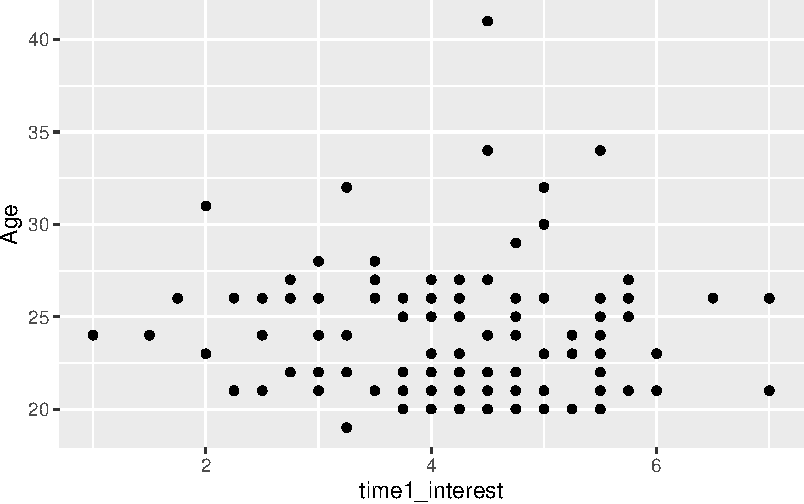
\includegraphics[width=1\textwidth,height=\textheight]{07-more-visualisation_files/figure-pdf/scat1-1.pdf}
\end{center}

\subsection{Activity 4 - Editing axis
labels}\label{activity-4---editing-axis-labels}

This plot is great for some exploratory data analysis, but it looks a
little untidy to put into a report. We can use the
\texttt{scale\_x\_continuous} and \texttt{scale\_y\_continuous} layers
to control the tick marks, as well as the axis name.

\begin{Shaded}
\begin{Highlighting}[]
\NormalTok{zhang\_data }\SpecialCharTok{\%\textgreater{}\%}  
  \FunctionTok{ggplot}\NormalTok{(}\FunctionTok{aes}\NormalTok{(}\AttributeTok{x =}\NormalTok{ time1\_interest,}\AttributeTok{y =}\NormalTok{ Age)) }\SpecialCharTok{+}
  \FunctionTok{geom\_point}\NormalTok{() }\SpecialCharTok{+}
  \FunctionTok{scale\_x\_continuous}\NormalTok{(}\AttributeTok{name =} \StringTok{"Time 1 interest score (1{-}7)"}\NormalTok{, }
                     \AttributeTok{breaks =} \FunctionTok{c}\NormalTok{(}\DecValTok{1}\SpecialCharTok{:}\DecValTok{7}\NormalTok{)) }\SpecialCharTok{+} \CommentTok{\# tick marks from 1 to 7}
  \FunctionTok{scale\_y\_continuous}\NormalTok{(}\AttributeTok{name =} \StringTok{"Age"}\NormalTok{,}
                     \AttributeTok{limits =} \FunctionTok{c}\NormalTok{(}\DecValTok{15}\NormalTok{, }\DecValTok{45}\NormalTok{), }\CommentTok{\# change limits to 15 to 45}
                     \AttributeTok{breaks =} \FunctionTok{seq}\NormalTok{(}\AttributeTok{from =} \DecValTok{15}\NormalTok{, }\CommentTok{\# sequence from 15}
                                  \AttributeTok{to =} \DecValTok{45}\NormalTok{, }\CommentTok{\# to 45 }
                                  \AttributeTok{by =} \DecValTok{5}\NormalTok{)) }\CommentTok{\# in steps of 5}
\end{Highlighting}
\end{Shaded}

\begin{center}
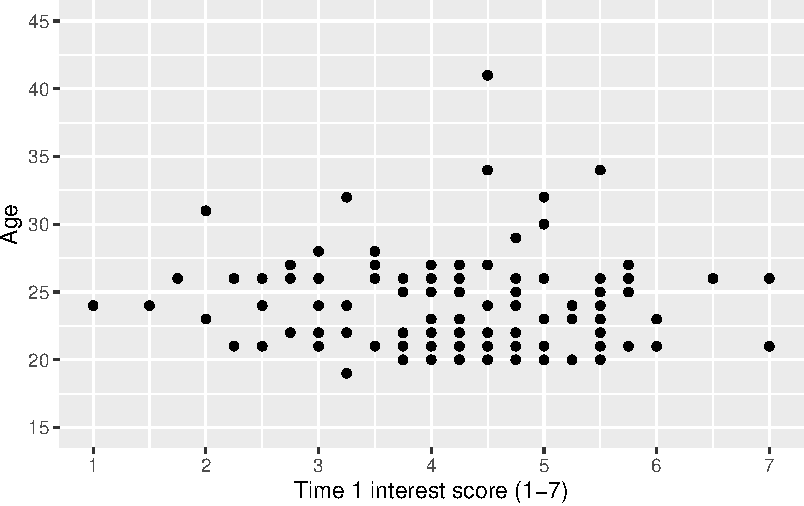
\includegraphics[width=1\textwidth,height=\textheight]{07-more-visualisation_files/figure-pdf/scat2-1.pdf}
\end{center}

To break down these new arguments/functions in the layers:

\begin{itemize}
\item
  \texttt{breaks} set the tick marks on the plot. We demonstrate two
  ways of setting this. On the x-axis, we just manually set values for 1
  to 7. On the y-axis, we use a second function to set the breaks.
\item
  \texttt{seq()} creates a sequence of numbers and can save a lot of
  time when you need to add lots of values. We set three arguments,
  \texttt{from} for the starting point, \texttt{to} for the end point,
  and \texttt{by} for the steps the sequence goes up in.
\item
  \texttt{limits} controls the start and end point of the graph scale.
  In the original graph, we can see there are points below 20 and above
  40, so we might want to increase the \texttt{limits} of the graph to
  include a wider range.
\end{itemize}

\begin{tcolorbox}[enhanced jigsaw, breakable, colframe=quarto-callout-important-color-frame, arc=.35mm, opacitybacktitle=0.6, titlerule=0mm, colbacktitle=quarto-callout-important-color!10!white, colback=white, toprule=.15mm, bottomtitle=1mm, toptitle=1mm, title=\textcolor{quarto-callout-important-color}{\faExclamation}\hspace{0.5em}{Error mode}, bottomrule=.15mm, rightrule=.15mm, leftrule=.75mm, coltitle=black, left=2mm, opacityback=0]

When controlling the limits of the graph, sometimes you want to decrease
the \texttt{limits} range to zoom in on an element of the data. If you
decrease the range which cuts off some data points, you must be very
careful as it actually cuts off data which you would receive a warning
about:

\begin{Shaded}
\begin{Highlighting}[]
\NormalTok{zhang\_data }\SpecialCharTok{\%\textgreater{}\%}  
  \FunctionTok{ggplot}\NormalTok{(}\FunctionTok{aes}\NormalTok{(}\AttributeTok{x =}\NormalTok{ time1\_interest,}\AttributeTok{y =}\NormalTok{ Age)) }\SpecialCharTok{+}
  \FunctionTok{geom\_point}\NormalTok{() }\SpecialCharTok{+}
  \FunctionTok{scale\_y\_continuous}\NormalTok{(}\AttributeTok{name =} \StringTok{"Age"}\NormalTok{,}
                     \AttributeTok{limits =} \FunctionTok{c}\NormalTok{(}\DecValTok{30}\NormalTok{, }\DecValTok{40}\NormalTok{)) }\CommentTok{\# in steps of 5}
\end{Highlighting}
\end{Shaded}

\begin{verbatim}
Warning: Removed 124 rows containing missing values or values outside the scale range
(`geom_point()`).
\end{verbatim}

\begin{center}
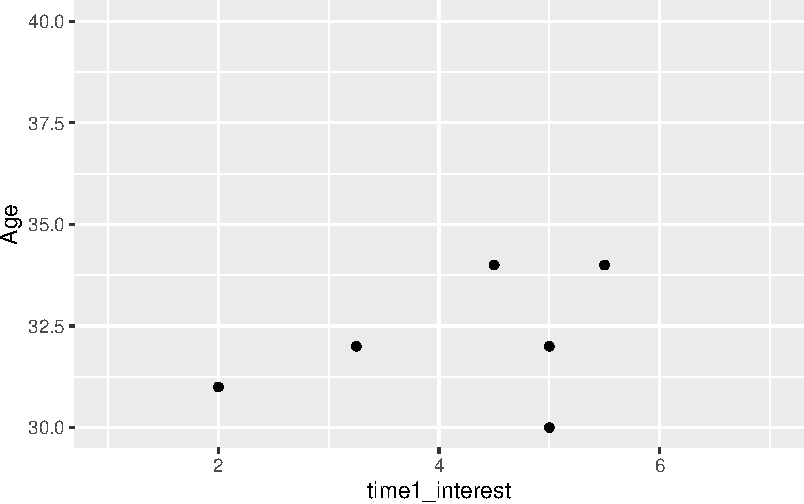
\includegraphics[width=1\textwidth,height=\textheight]{07-more-visualisation_files/figure-pdf/unnamed-chunk-2-1.pdf}
\end{center}

You must be very careful when truncating axes, but if you \emph{do} need
to do it, there is a different function layer to use:

\begin{Shaded}
\begin{Highlighting}[]
\NormalTok{zhang\_data }\SpecialCharTok{\%\textgreater{}\%}  
  \FunctionTok{ggplot}\NormalTok{(}\FunctionTok{aes}\NormalTok{(}\AttributeTok{x =}\NormalTok{ time1\_interest,}\AttributeTok{y =}\NormalTok{ Age)) }\SpecialCharTok{+}
  \FunctionTok{geom\_point}\NormalTok{() }\SpecialCharTok{+}
  \FunctionTok{coord\_cartesian}\NormalTok{(}\AttributeTok{ylim =} \FunctionTok{c}\NormalTok{(}\DecValTok{30}\NormalTok{, }\DecValTok{40}\NormalTok{))}
\end{Highlighting}
\end{Shaded}

\begin{center}
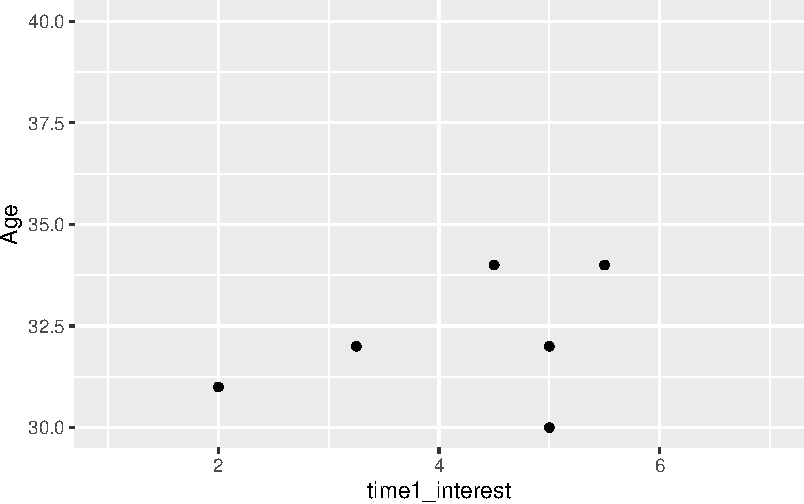
\includegraphics[width=1\textwidth,height=\textheight]{07-more-visualisation_files/figure-pdf/unnamed-chunk-3-1.pdf}
\end{center}

\end{tcolorbox}

\subsection{Activity 5 - Adding a regression
line}\label{activity-5---adding-a-regression-line}

It is often useful to add a regression line or line of best fit to a
scatterplot. You can add a regression line with the
\texttt{geom\_smooth()} layer and by default will also provide a 95\%
confidence interval ribbon. You can specify what type of line you want
to draw, most often you will need \texttt{method\ =\ "lm"} for a linear
model or a straight line.

\begin{Shaded}
\begin{Highlighting}[]
\NormalTok{zhang\_data }\SpecialCharTok{\%\textgreater{}\%}  
  \FunctionTok{ggplot}\NormalTok{(}\FunctionTok{aes}\NormalTok{(}\AttributeTok{x =}\NormalTok{ time1\_interest,}\AttributeTok{y =}\NormalTok{ Age)) }\SpecialCharTok{+}
  \FunctionTok{geom\_point}\NormalTok{() }\SpecialCharTok{+}
  \FunctionTok{scale\_x\_continuous}\NormalTok{(}\AttributeTok{name =} \StringTok{"Time 1 interest score (1{-}7)"}\NormalTok{, }
                     \AttributeTok{breaks =} \FunctionTok{c}\NormalTok{(}\DecValTok{1}\SpecialCharTok{:}\DecValTok{7}\NormalTok{)) }\SpecialCharTok{+} \CommentTok{\# tick marks from 1 to 7}
  \FunctionTok{scale\_y\_continuous}\NormalTok{(}\AttributeTok{name =} \StringTok{"Age"}\NormalTok{,}
                     \AttributeTok{limits =} \FunctionTok{c}\NormalTok{(}\DecValTok{15}\NormalTok{, }\DecValTok{45}\NormalTok{), }\CommentTok{\# change limits to 15 to 45}
                     \AttributeTok{breaks =} \FunctionTok{seq}\NormalTok{(}\AttributeTok{from =} \DecValTok{15}\NormalTok{, }\CommentTok{\# sequence from 15}
                                  \AttributeTok{to =} \DecValTok{45}\NormalTok{, }\CommentTok{\# to 45 }
                                  \AttributeTok{by =} \DecValTok{5}\NormalTok{)) }\SpecialCharTok{+}  \CommentTok{\# in steps of 5}
  \FunctionTok{geom\_smooth}\NormalTok{(}\AttributeTok{method =} \StringTok{"lm"}\NormalTok{)}
\end{Highlighting}
\end{Shaded}

\begin{center}
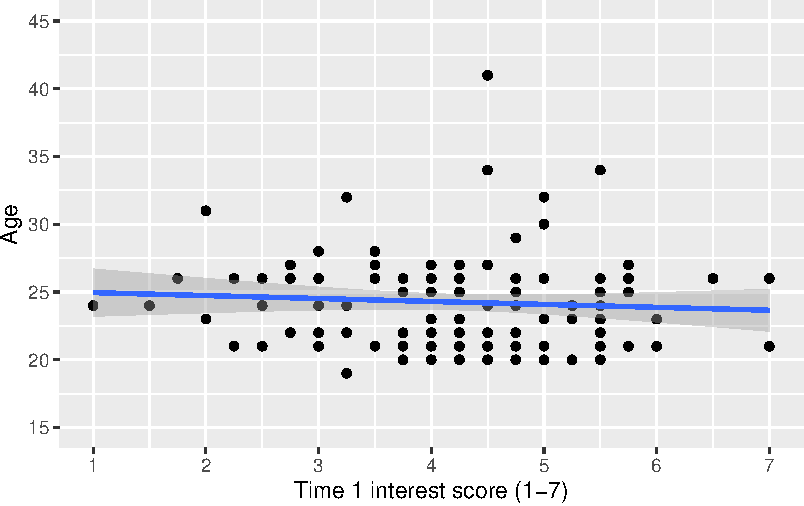
\includegraphics[width=1\textwidth,height=\textheight]{07-more-visualisation_files/figure-pdf/scat3-1.pdf}
\end{center}

With the regression line, we can see there is very little relationship
between age and interest score at time 1.

\begin{tcolorbox}[enhanced jigsaw, breakable, colframe=quarto-callout-important-color-frame, arc=.35mm, opacitybacktitle=0.6, titlerule=0mm, colbacktitle=quarto-callout-important-color!10!white, colback=white, toprule=.15mm, bottomtitle=1mm, toptitle=1mm, title=\textcolor{quarto-callout-important-color}{\faExclamation}\hspace{0.5em}{Important}, bottomrule=.15mm, rightrule=.15mm, leftrule=.75mm, coltitle=black, left=2mm, opacityback=0]

Remember, you can save your plots using the function \texttt{ggsave()}.
You can use the function after creating the last plot, or saving your
plot as an object and using the \texttt{plot} argument. You have a
\texttt{Figures/} directory for the chapter, so try and save the plots
you make to remind yourself later.

\end{tcolorbox}

\begin{tcolorbox}[enhanced jigsaw, breakable, colframe=quarto-callout-tip-color-frame, arc=.35mm, opacitybacktitle=0.6, titlerule=0mm, colbacktitle=quarto-callout-tip-color!10!white, colback=white, toprule=.15mm, bottomtitle=1mm, toptitle=1mm, title=\textcolor{quarto-callout-tip-color}{\faLightbulb}\hspace{0.5em}{Try this}, bottomrule=.15mm, rightrule=.15mm, leftrule=.75mm, coltitle=black, left=2mm, opacityback=0]

So far, we made a scatterplot of age against interest at time 1. Now,
create a scatterplot on your own using the two interest rating
variables: \texttt{time1\_interest} and \texttt{time2\_interest}.

After you made the scatterplot, it looks like there is a

\begin{itemize}
\tightlist
\item
  \begin{enumerate}
  \def\labelenumi{(\Alph{enumi})}
  \tightlist
  \item
    positive\\
  \end{enumerate}
\item
  \begin{enumerate}
  \def\labelenumi{(\Alph{enumi})}
  \setcounter{enumi}{1}
  \tightlist
  \item
    negative
  \end{enumerate}
\end{itemize}

relationship between interest ratings at time 1 and time 2.

\end{tcolorbox}

\begin{tcolorbox}[enhanced jigsaw, breakable, colframe=quarto-callout-caution-color-frame, arc=.35mm, opacitybacktitle=0.6, titlerule=0mm, colbacktitle=quarto-callout-caution-color!10!white, colback=white, toprule=.15mm, bottomtitle=1mm, toptitle=1mm, title=\textcolor{quarto-callout-caution-color}{\faFire}\hspace{0.5em}{Show me the solution}, bottomrule=.15mm, rightrule=.15mm, leftrule=.75mm, coltitle=black, left=2mm, opacityback=0]

You should have the following in a code chunk:

\begin{Shaded}
\begin{Highlighting}[]
\NormalTok{zhang\_data }\SpecialCharTok{\%\textgreater{}\%}  
  \FunctionTok{ggplot}\NormalTok{(}\FunctionTok{aes}\NormalTok{(}\AttributeTok{x =}\NormalTok{ time1\_interest, }\AttributeTok{y =}\NormalTok{ time2\_interest)) }\SpecialCharTok{+}
  \FunctionTok{geom\_point}\NormalTok{() }\SpecialCharTok{+}
  \FunctionTok{scale\_x\_continuous}\NormalTok{(}\AttributeTok{name =} \StringTok{"Time 1 interest score (1{-}7)"}\NormalTok{, }
                     \AttributeTok{breaks =} \FunctionTok{c}\NormalTok{(}\DecValTok{1}\SpecialCharTok{:}\DecValTok{7}\NormalTok{)) }\SpecialCharTok{+} \CommentTok{\# tick marks from 1 to 7}
  \FunctionTok{scale\_y\_continuous}\NormalTok{(}\AttributeTok{name =} \StringTok{"Time 2 interest score (1{-}7)"}\NormalTok{, }
                     \AttributeTok{breaks =} \FunctionTok{c}\NormalTok{(}\DecValTok{1}\SpecialCharTok{:}\DecValTok{7}\NormalTok{)) }\SpecialCharTok{+} \CommentTok{\# tick marks from 1 to 7}
  \FunctionTok{geom\_smooth}\NormalTok{(}\AttributeTok{method =} \StringTok{"lm"}\NormalTok{)}
\end{Highlighting}
\end{Shaded}

\begin{center}
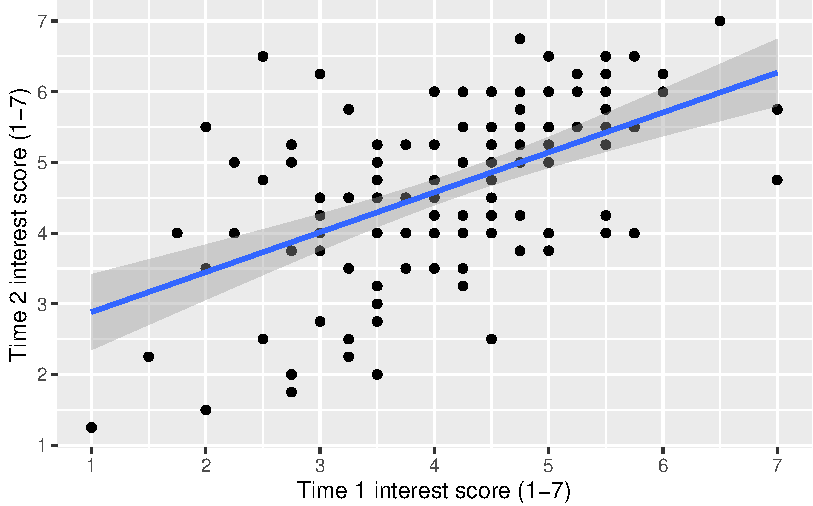
\includegraphics[width=1\textwidth,height=\textheight]{07-more-visualisation_files/figure-pdf/unnamed-chunk-4-1.pdf}
\end{center}

\end{tcolorbox}

\subsection{Activity 6 - Creating a grouped
scatterplot}\label{activity-6---creating-a-grouped-scatterplot}

Before we move on, we can add a third variable to show how the
relationship might differ for different groups within our data. We can
do this by adding the \texttt{colour} argument to \texttt{aes()} and
setting it as whatever variable we would like to distinguish between. In
this case, we will see how the relationship between age and interest at
time 1 differs for the male and female participants. There are a few
participants with missing gender, so we will first filter them out.

\begin{Shaded}
\begin{Highlighting}[]
\NormalTok{zhang\_data }\SpecialCharTok{\%\textgreater{}\%}
  \FunctionTok{drop\_na}\NormalTok{(Gender) }\SpecialCharTok{\%\textgreater{}\%} 
  \FunctionTok{ggplot}\NormalTok{(}\FunctionTok{aes}\NormalTok{(}\AttributeTok{x =}\NormalTok{ time1\_interest, }\AttributeTok{y =}\NormalTok{ Age, }\AttributeTok{colour =}\NormalTok{ Gender)) }\SpecialCharTok{+}
  \FunctionTok{geom\_point}\NormalTok{() }\SpecialCharTok{+}
  \FunctionTok{scale\_x\_continuous}\NormalTok{(}\AttributeTok{name =} \StringTok{"Mean interest score (1{-}7)"}\NormalTok{,}
                     \AttributeTok{breaks =} \FunctionTok{c}\NormalTok{(}\DecValTok{1}\SpecialCharTok{:}\DecValTok{7}\NormalTok{)) }\SpecialCharTok{+} 
  \FunctionTok{scale\_y\_continuous}\NormalTok{(}\AttributeTok{name =} \StringTok{"Age"}\NormalTok{) }\SpecialCharTok{+}
  \FunctionTok{geom\_smooth}\NormalTok{(}\AttributeTok{method =} \StringTok{"lm"}\NormalTok{)}
\end{Highlighting}
\end{Shaded}

\begin{figure}[H]

{\centering 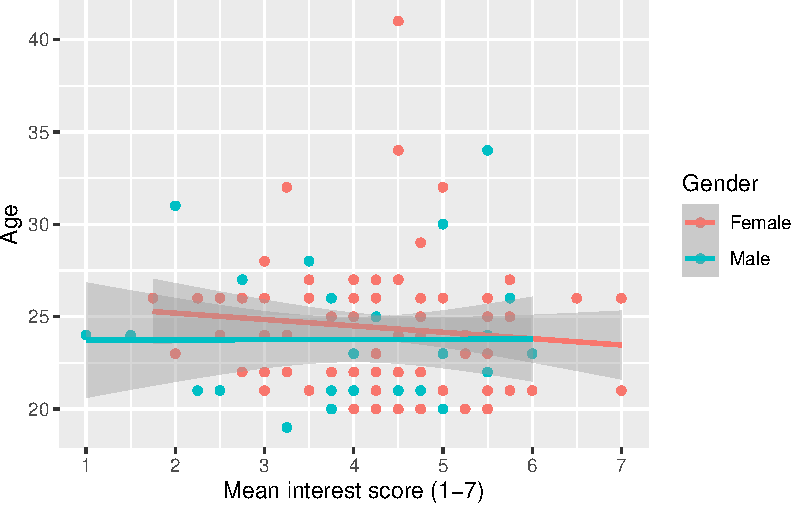
\includegraphics[width=1\textwidth,height=\textheight]{07-more-visualisation_files/figure-pdf/scat4-1.pdf}

}

\caption{Grouped scatterplot}

\end{figure}%

\begin{tcolorbox}[enhanced jigsaw, breakable, colframe=quarto-callout-tip-color-frame, arc=.35mm, opacitybacktitle=0.6, titlerule=0mm, colbacktitle=quarto-callout-tip-color!10!white, colback=white, toprule=.15mm, bottomtitle=1mm, toptitle=1mm, title=\textcolor{quarto-callout-tip-color}{\faLightbulb}\hspace{0.5em}{Try this}, bottomrule=.15mm, rightrule=.15mm, leftrule=.75mm, coltitle=black, left=2mm, opacityback=0]

For your independent scatterplot of the two interest rating variables:
\texttt{time1\_interest} and \texttt{time2\_interest}, add a
\texttt{colour} argument using the \texttt{Condition} variable. This
will show the relationship between time 1 and time 2 interest separately
for participants in the ordinary and extraordinary groups.

\end{tcolorbox}

\begin{tcolorbox}[enhanced jigsaw, breakable, colframe=quarto-callout-caution-color-frame, arc=.35mm, opacitybacktitle=0.6, titlerule=0mm, colbacktitle=quarto-callout-caution-color!10!white, colback=white, toprule=.15mm, bottomtitle=1mm, toptitle=1mm, title=\textcolor{quarto-callout-caution-color}{\faFire}\hspace{0.5em}{Show me the solution}, bottomrule=.15mm, rightrule=.15mm, leftrule=.75mm, coltitle=black, left=2mm, opacityback=0]

You should have the following in a code chunk:

\begin{Shaded}
\begin{Highlighting}[]
\NormalTok{zhang\_data }\SpecialCharTok{\%\textgreater{}\%}  
  \FunctionTok{ggplot}\NormalTok{(}\FunctionTok{aes}\NormalTok{(}\AttributeTok{x =}\NormalTok{ time1\_interest, }\AttributeTok{y =}\NormalTok{ time2\_interest, }\AttributeTok{colour =}\NormalTok{ Condition)) }\SpecialCharTok{+}
  \FunctionTok{geom\_point}\NormalTok{() }\SpecialCharTok{+}
  \FunctionTok{scale\_x\_continuous}\NormalTok{(}\AttributeTok{name =} \StringTok{"Time 1 interest score (1{-}7)"}\NormalTok{, }
                     \AttributeTok{breaks =} \FunctionTok{c}\NormalTok{(}\DecValTok{1}\SpecialCharTok{:}\DecValTok{7}\NormalTok{)) }\SpecialCharTok{+} \CommentTok{\# tick marks from 1 to 7}
  \FunctionTok{scale\_y\_continuous}\NormalTok{(}\AttributeTok{name =} \StringTok{"Time 2 interest score (1{-}7)"}\NormalTok{, }
                     \AttributeTok{breaks =} \FunctionTok{c}\NormalTok{(}\DecValTok{1}\SpecialCharTok{:}\DecValTok{7}\NormalTok{)) }\SpecialCharTok{+} \CommentTok{\# tick marks from 1 to 7}
  \FunctionTok{geom\_smooth}\NormalTok{(}\AttributeTok{method =} \StringTok{"lm"}\NormalTok{)}
\end{Highlighting}
\end{Shaded}

\begin{center}
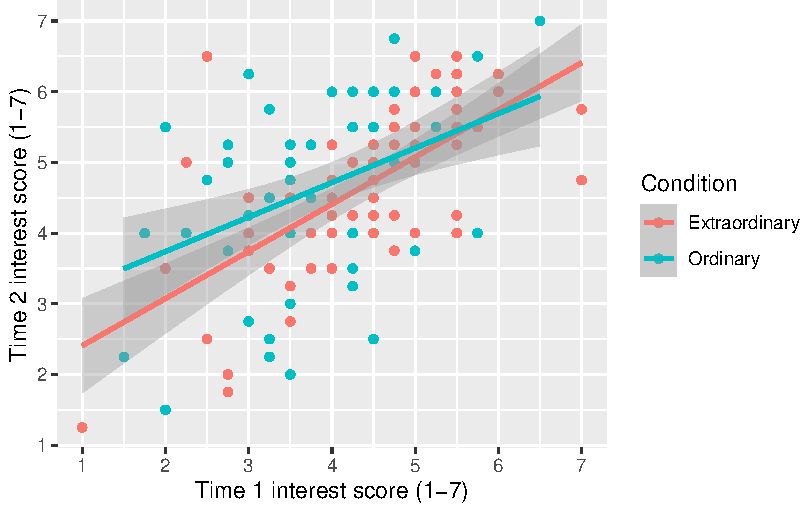
\includegraphics[width=1\textwidth,height=\textheight]{07-more-visualisation_files/figure-pdf/unnamed-chunk-5-1.pdf}
\end{center}

\end{tcolorbox}

\section{Boxplots}\label{viz-a4}

The next visualisation is the boxplot which presents a range of summary
statistics for your outcome, which you can split between different
groups on the x-axis, or add further variables to divide by. For the
boxplot element, you get five summary statistics: the median centre
line, the first and third quartile as the box (essentially, the
interquartile range), and 1.5 times the first and third quartiles as the
whiskers extending from the box. If there are any values beyond the
whiskers, you see the individual data points and this is one definition
of an outlier (more on that in Chapter 11)

\subsection{Activity 7 - Creating a basic
boxplot}\label{activity-7---creating-a-basic-boxplot}

Before we create the boxplot, we need a final data wrangling step. At
the moment, we have \texttt{time1\_interest} and
\texttt{time2\_interest} in wide format, but to plot together, we need
to express it as a single variable. For that, we must restructure the
data. This is why we spent so much time on data wrangling, as you might
need to quickly restructure your data to plot certain elements.

\begin{tcolorbox}[enhanced jigsaw, breakable, colframe=quarto-callout-tip-color-frame, arc=.35mm, opacitybacktitle=0.6, titlerule=0mm, colbacktitle=quarto-callout-tip-color!10!white, colback=white, toprule=.15mm, bottomtitle=1mm, toptitle=1mm, title=\textcolor{quarto-callout-tip-color}{\faLightbulb}\hspace{0.5em}{Try this}, bottomrule=.15mm, rightrule=.15mm, leftrule=.75mm, coltitle=black, left=2mm, opacityback=0]

To wrangle the data, gather the variables \texttt{time1\_interest} and
\texttt{time2\_interest}. Create a new object called
\texttt{zhang\_data\_long} and use the names \texttt{Time} and
\texttt{Interest} for your column names to be consistent with the
demonstrations below.

\end{tcolorbox}

\begin{tcolorbox}[enhanced jigsaw, breakable, colframe=quarto-callout-caution-color-frame, arc=.35mm, opacitybacktitle=0.6, titlerule=0mm, colbacktitle=quarto-callout-caution-color!10!white, colback=white, toprule=.15mm, bottomtitle=1mm, toptitle=1mm, title=\textcolor{quarto-callout-caution-color}{\faFire}\hspace{0.5em}{Show me the solution}, bottomrule=.15mm, rightrule=.15mm, leftrule=.75mm, coltitle=black, left=2mm, opacityback=0]

You should have the following in a code chunk:

\begin{Shaded}
\begin{Highlighting}[]
\CommentTok{\# gather the data to convert to long format}
\NormalTok{zhang\_data\_long }\OtherTok{\textless{}{-}}\NormalTok{ zhang\_data }\SpecialCharTok{\%\textgreater{}\%} 
  \FunctionTok{pivot\_longer}\NormalTok{(}\AttributeTok{cols =}\NormalTok{ time1\_interest}\SpecialCharTok{:}\NormalTok{time2\_interest,}
               \AttributeTok{names\_to =} \StringTok{"Time"}\NormalTok{,}
               \AttributeTok{values\_to =} \StringTok{"Interest"}\NormalTok{)}
\end{Highlighting}
\end{Shaded}

\end{tcolorbox}

If you only want to visualise one continuous variable, we need one
variable on the y-axis and a new function layer
\texttt{geom\_boxplot()}.

\begin{Shaded}
\begin{Highlighting}[]
\NormalTok{zhang\_data\_long }\SpecialCharTok{\%\textgreater{}\%} 
  \FunctionTok{ggplot}\NormalTok{(}\FunctionTok{aes}\NormalTok{(}\AttributeTok{y =}\NormalTok{ Interest)) }\SpecialCharTok{+}
  \FunctionTok{geom\_boxplot}\NormalTok{() }\SpecialCharTok{+} 
  \FunctionTok{scale\_y\_continuous}\NormalTok{(}\AttributeTok{name =} \StringTok{"Interest score (1{-}7)"}\NormalTok{, }
                     \AttributeTok{breaks =} \FunctionTok{c}\NormalTok{(}\DecValTok{1}\SpecialCharTok{:}\DecValTok{7}\NormalTok{))}
\end{Highlighting}
\end{Shaded}

\begin{center}
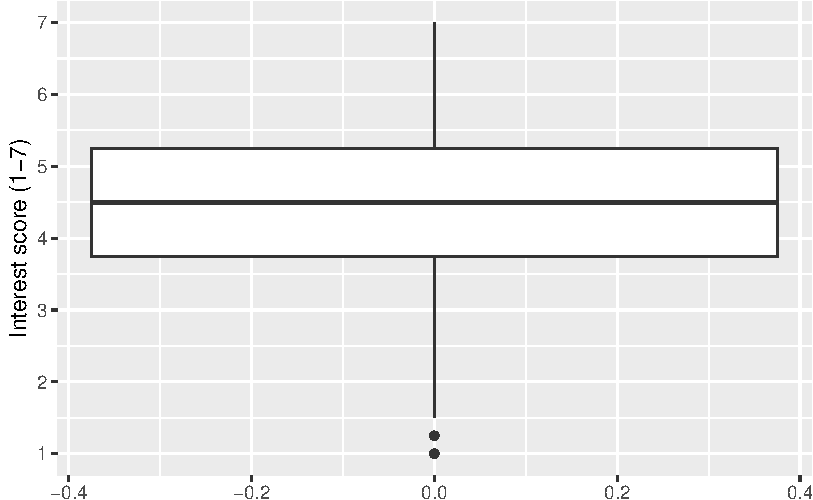
\includegraphics[width=1\textwidth,height=\textheight]{07-more-visualisation_files/figure-pdf/bp1-1.pdf}
\end{center}

Typically, you want to compare the outcome between one or more
categories, so we can add a categorical variable like gender to the
x-axis, removing the missing values first.

\begin{Shaded}
\begin{Highlighting}[]
\NormalTok{zhang\_data\_long }\SpecialCharTok{\%\textgreater{}\%} 
  \FunctionTok{drop\_na}\NormalTok{(Gender) }\SpecialCharTok{\%\textgreater{}\%} 
  \FunctionTok{ggplot}\NormalTok{(}\FunctionTok{aes}\NormalTok{(}\AttributeTok{y =}\NormalTok{ Interest, }\AttributeTok{x =}\NormalTok{ Gender)) }\SpecialCharTok{+}
  \FunctionTok{geom\_boxplot}\NormalTok{() }\SpecialCharTok{+} 
  \FunctionTok{scale\_y\_continuous}\NormalTok{(}\AttributeTok{name =} \StringTok{"Interest score (1{-}7)"}\NormalTok{, }
                     \AttributeTok{breaks =} \FunctionTok{c}\NormalTok{(}\DecValTok{1}\SpecialCharTok{:}\DecValTok{7}\NormalTok{))}
\end{Highlighting}
\end{Shaded}

\begin{center}
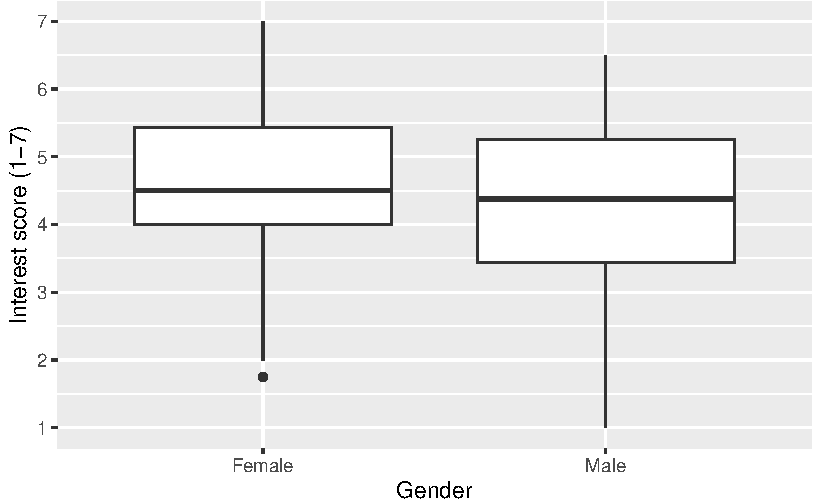
\includegraphics[width=1\textwidth,height=\textheight]{07-more-visualisation_files/figure-pdf/unnamed-chunk-7-1.pdf}
\end{center}

\subsection{Activity 8 - Adding colour to
variables}\label{activity-8---adding-colour-to-variables}

It is not as important when you only have one variable on the x-axis,
but one useful feature is adding colour to distinguish between
categories. You can control this by adding a variable to the
\texttt{fill} argument within \texttt{aes()}.

By default, we get a legend which is redundant when we only have
different colours on the x-axis, so we can turn it off by adding
\texttt{guides(fill\ =\ FALSE)} as a layer.

\begin{Shaded}
\begin{Highlighting}[]
\NormalTok{zhang\_data\_long }\SpecialCharTok{\%\textgreater{}\%} 
  \FunctionTok{drop\_na}\NormalTok{(Gender) }\SpecialCharTok{\%\textgreater{}\%} 
  \FunctionTok{ggplot}\NormalTok{(}\FunctionTok{aes}\NormalTok{(}\AttributeTok{y =}\NormalTok{ Interest, }\AttributeTok{x =}\NormalTok{ Gender, }\AttributeTok{fill =}\NormalTok{ Gender)) }\SpecialCharTok{+}
  \FunctionTok{geom\_boxplot}\NormalTok{() }\SpecialCharTok{+} 
  \FunctionTok{scale\_y\_continuous}\NormalTok{(}\AttributeTok{name =} \StringTok{"Interest score (1{-}7)"}\NormalTok{, }
                     \AttributeTok{breaks =} \FunctionTok{c}\NormalTok{(}\DecValTok{1}\SpecialCharTok{:}\DecValTok{7}\NormalTok{)) }\SpecialCharTok{+} 
  \FunctionTok{guides}\NormalTok{(}\AttributeTok{fill =} \ConstantTok{FALSE}\NormalTok{) }\CommentTok{\# remove the legend}
\end{Highlighting}
\end{Shaded}

\begin{center}
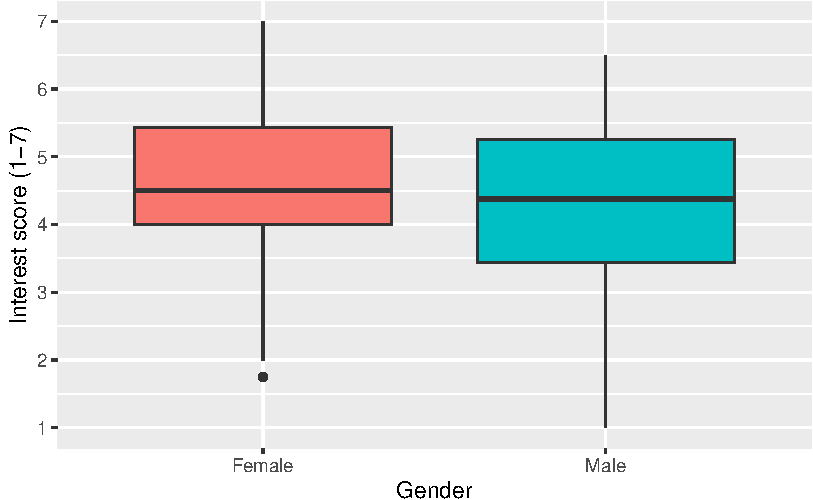
\includegraphics[width=1\textwidth,height=\textheight]{07-more-visualisation_files/figure-pdf/bp4-1.pdf}
\end{center}

\begin{tcolorbox}[enhanced jigsaw, breakable, colframe=quarto-callout-important-color-frame, arc=.35mm, opacitybacktitle=0.6, titlerule=0mm, colbacktitle=quarto-callout-important-color!10!white, colback=white, toprule=.15mm, bottomtitle=1mm, toptitle=1mm, title=\textcolor{quarto-callout-important-color}{\faExclamation}\hspace{0.5em}{Error mode}, bottomrule=.15mm, rightrule=.15mm, leftrule=.75mm, coltitle=black, left=2mm, opacityback=0]

You might have noticed we have now used two different arguments to
control the colour. In scatterplots, we used \texttt{colour}. In
boxplots, we used \texttt{fill}. It is one of those concepts that takes
time to recognise which you need, depending on the type of geom you are
using. Roughly, \texttt{colour} is when you want to control the outline
or symbol, like the points. Whereas \texttt{fill} is when you want the
inside of a geom coloured. You can see the difference here by
controlling \texttt{fill} first:

\begin{Shaded}
\begin{Highlighting}[]
\NormalTok{zhang\_data\_long }\SpecialCharTok{\%\textgreater{}\%} 
  \FunctionTok{drop\_na}\NormalTok{(Gender) }\SpecialCharTok{\%\textgreater{}\%} 
  \FunctionTok{ggplot}\NormalTok{(}\FunctionTok{aes}\NormalTok{(}\AttributeTok{y =}\NormalTok{ Interest, }\AttributeTok{x =}\NormalTok{ Gender, }\AttributeTok{fill =}\NormalTok{ Gender)) }\SpecialCharTok{+}
  \FunctionTok{geom\_boxplot}\NormalTok{() }\SpecialCharTok{+} 
  \FunctionTok{scale\_y\_continuous}\NormalTok{(}\AttributeTok{name =} \StringTok{"Interest score (1{-}7)"}\NormalTok{, }
                     \AttributeTok{breaks =} \FunctionTok{c}\NormalTok{(}\DecValTok{1}\SpecialCharTok{:}\DecValTok{7}\NormalTok{))}
\end{Highlighting}
\end{Shaded}

\begin{center}
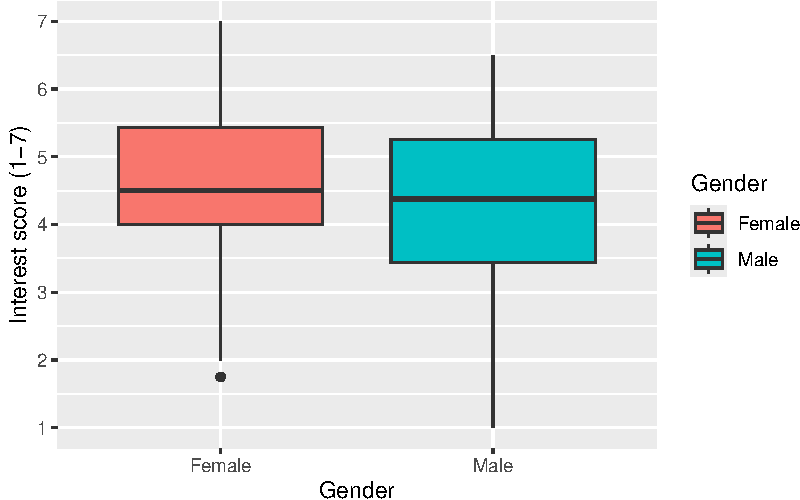
\includegraphics[width=1\textwidth,height=\textheight]{07-more-visualisation_files/figure-pdf/unnamed-chunk-8-1.pdf}
\end{center}

Then \texttt{colour}:

\begin{Shaded}
\begin{Highlighting}[]
\NormalTok{zhang\_data\_long }\SpecialCharTok{\%\textgreater{}\%} 
  \FunctionTok{drop\_na}\NormalTok{(Gender) }\SpecialCharTok{\%\textgreater{}\%} 
  \FunctionTok{ggplot}\NormalTok{(}\FunctionTok{aes}\NormalTok{(}\AttributeTok{y =}\NormalTok{ Interest, }\AttributeTok{x =}\NormalTok{ Gender, }\AttributeTok{colour =}\NormalTok{ Gender)) }\SpecialCharTok{+}
  \FunctionTok{geom\_boxplot}\NormalTok{() }\SpecialCharTok{+} 
  \FunctionTok{scale\_y\_continuous}\NormalTok{(}\AttributeTok{name =} \StringTok{"Interest score (1{-}7)"}\NormalTok{, }
                     \AttributeTok{breaks =} \FunctionTok{c}\NormalTok{(}\DecValTok{1}\SpecialCharTok{:}\DecValTok{7}\NormalTok{))}
\end{Highlighting}
\end{Shaded}

\begin{center}
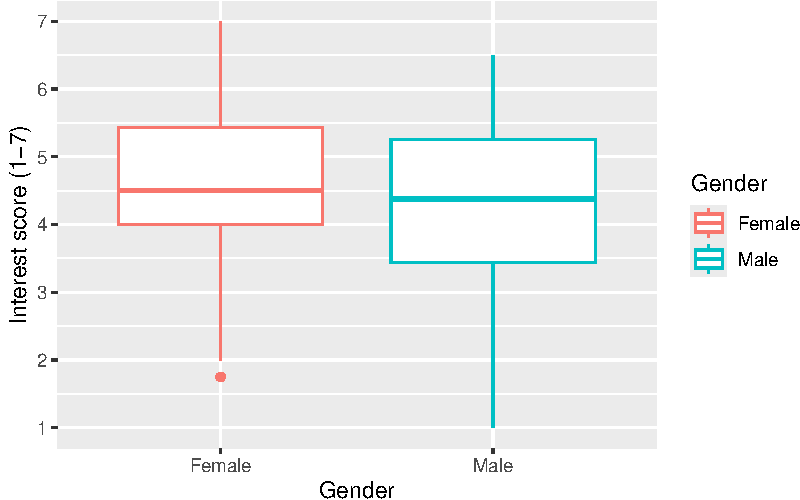
\includegraphics[width=1\textwidth,height=\textheight]{07-more-visualisation_files/figure-pdf/unnamed-chunk-9-1.pdf}
\end{center}

\end{tcolorbox}

\subsection{Activity 9 - Controlling
colours}\label{activity-9---controlling-colours}

ggplot2 has a default colour scheme which is fine for quick plots, but
it is useful to control the colour scheme. You can do this manually by
editing \texttt{scale\_fill\_discrete()} and choosing colours through
the \texttt{type} argument (you can do this through character names or
choosing a HEX code: \url{https://r-charts.com/colors/}).

\begin{Shaded}
\begin{Highlighting}[]
\NormalTok{zhang\_data\_long }\SpecialCharTok{\%\textgreater{}\%} 
  \FunctionTok{drop\_na}\NormalTok{(Gender) }\SpecialCharTok{\%\textgreater{}\%} 
  \FunctionTok{ggplot}\NormalTok{(}\FunctionTok{aes}\NormalTok{(}\AttributeTok{y =}\NormalTok{ Interest, }\AttributeTok{x =}\NormalTok{ Gender, }\AttributeTok{fill =}\NormalTok{ Gender)) }\SpecialCharTok{+}
  \FunctionTok{geom\_boxplot}\NormalTok{() }\SpecialCharTok{+} 
  \FunctionTok{scale\_y\_continuous}\NormalTok{(}\AttributeTok{name =} \StringTok{"Interest score (1{-}7)"}\NormalTok{, }
                     \AttributeTok{breaks =} \FunctionTok{c}\NormalTok{(}\DecValTok{1}\SpecialCharTok{:}\DecValTok{7}\NormalTok{)) }\SpecialCharTok{+} 
  \FunctionTok{scale\_fill\_discrete}\NormalTok{(}\AttributeTok{type =} \FunctionTok{c}\NormalTok{(}\StringTok{"blue"}\NormalTok{, }\StringTok{"pink"}\NormalTok{))}
\end{Highlighting}
\end{Shaded}

\begin{center}
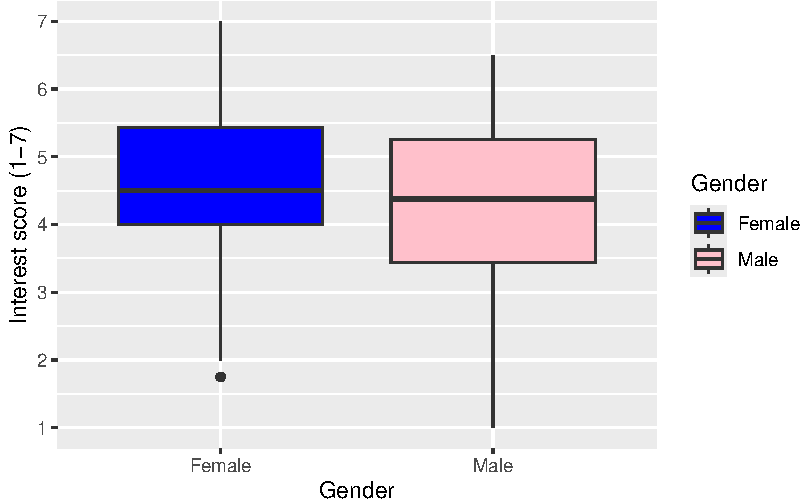
\includegraphics[width=1\textwidth,height=\textheight]{07-more-visualisation_files/figure-pdf/unnamed-chunk-10-1.pdf}
\end{center}

Alternatively (and what we recommend), you can use
\texttt{scale\_fill\_viridis\_d()}. This function does exactly the same
thing but it uses a colour-blind friendly palette (which also prints in
black and white). There are 5 different options for colours and you can
see them by changing \texttt{option} to A, B, C, D or E. We like option
E with \texttt{alpha\ =\ 0.6} (to control transparency and soften the
tone) but play around with the options to see what you prefer.

\begin{Shaded}
\begin{Highlighting}[]
\NormalTok{zhang\_data\_long }\SpecialCharTok{\%\textgreater{}\%} 
  \FunctionTok{drop\_na}\NormalTok{(Gender) }\SpecialCharTok{\%\textgreater{}\%} 
  \FunctionTok{ggplot}\NormalTok{(}\FunctionTok{aes}\NormalTok{(}\AttributeTok{y =}\NormalTok{ Interest, }\AttributeTok{x =}\NormalTok{ Gender, }\AttributeTok{fill =}\NormalTok{ Gender)) }\SpecialCharTok{+}
  \FunctionTok{geom\_boxplot}\NormalTok{() }\SpecialCharTok{+} 
  \FunctionTok{scale\_y\_continuous}\NormalTok{(}\AttributeTok{name =} \StringTok{"Interest score (1{-}7)"}\NormalTok{, }
                     \AttributeTok{breaks =} \FunctionTok{c}\NormalTok{(}\DecValTok{1}\SpecialCharTok{:}\DecValTok{7}\NormalTok{)) }\SpecialCharTok{+} 
  \FunctionTok{scale\_fill\_viridis\_d}\NormalTok{(}\AttributeTok{option =} \StringTok{"E"}\NormalTok{, }
                       \AttributeTok{alpha =} \FloatTok{0.6}\NormalTok{) }\SpecialCharTok{+} 
  \FunctionTok{guides}\NormalTok{(}\AttributeTok{fill =} \StringTok{"none"}\NormalTok{)}
\end{Highlighting}
\end{Shaded}

\begin{figure}[H]

{\centering 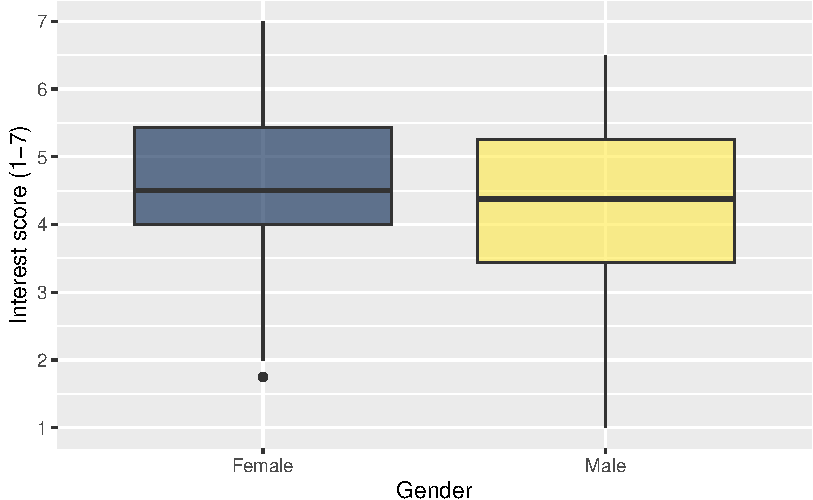
\includegraphics[width=1\textwidth,height=\textheight]{07-more-visualisation_files/figure-pdf/unnamed-chunk-11-1.pdf}

}

\caption{Boxplots with friendly colours}

\end{figure}%

\begin{tcolorbox}[enhanced jigsaw, breakable, colframe=quarto-callout-tip-color-frame, arc=.35mm, opacitybacktitle=0.6, titlerule=0mm, colbacktitle=quarto-callout-tip-color!10!white, colback=white, toprule=.15mm, bottomtitle=1mm, toptitle=1mm, title=\textcolor{quarto-callout-tip-color}{\faLightbulb}\hspace{0.5em}{Try this}, bottomrule=.15mm, rightrule=.15mm, leftrule=.75mm, coltitle=black, left=2mm, opacityback=0]

For your independent boxplot, use \texttt{zhang\_data\_long} to
visualise \texttt{Interest} as your continuous variable and
\texttt{Condition} for different categories. This will show the
difference in interest rating between those in the ordinary and
extraordinary groups.

Comparing the ordinary and extraordinary groups, it looks like

\begin{itemize}
\tightlist
\item
  \begin{enumerate}
  \def\labelenumi{(\Alph{enumi})}
  \tightlist
  \item
    ordinary score higher on average\\
  \end{enumerate}
\item
  \begin{enumerate}
  \def\labelenumi{(\Alph{enumi})}
  \setcounter{enumi}{1}
  \tightlist
  \item
    very little difference on average\\
  \end{enumerate}
\item
  \begin{enumerate}
  \def\labelenumi{(\Alph{enumi})}
  \setcounter{enumi}{2}
  \tightlist
  \item
    extraordinary score higher on average
  \end{enumerate}
\end{itemize}

.

\end{tcolorbox}

\begin{tcolorbox}[enhanced jigsaw, breakable, colframe=quarto-callout-caution-color-frame, arc=.35mm, opacitybacktitle=0.6, titlerule=0mm, colbacktitle=quarto-callout-caution-color!10!white, colback=white, toprule=.15mm, bottomtitle=1mm, toptitle=1mm, title=\textcolor{quarto-callout-caution-color}{\faFire}\hspace{0.5em}{Show me the solution}, bottomrule=.15mm, rightrule=.15mm, leftrule=.75mm, coltitle=black, left=2mm, opacityback=0]

You should have the following in a code chunk:

\begin{Shaded}
\begin{Highlighting}[]
\NormalTok{zhang\_data\_long }\SpecialCharTok{\%\textgreater{}\%} 
  \FunctionTok{ggplot}\NormalTok{(}\FunctionTok{aes}\NormalTok{(}\AttributeTok{y =}\NormalTok{ Interest, }\AttributeTok{x =}\NormalTok{ Condition, }\AttributeTok{fill =}\NormalTok{ Condition)) }\SpecialCharTok{+}
  \FunctionTok{geom\_boxplot}\NormalTok{() }\SpecialCharTok{+} 
  \FunctionTok{scale\_y\_continuous}\NormalTok{(}\AttributeTok{name =} \StringTok{"Interest score (1{-}7)"}\NormalTok{, }
                     \AttributeTok{breaks =} \FunctionTok{c}\NormalTok{(}\DecValTok{1}\SpecialCharTok{:}\DecValTok{7}\NormalTok{)) }\SpecialCharTok{+} 
  \FunctionTok{scale\_fill\_viridis\_d}\NormalTok{(}\AttributeTok{option =} \StringTok{"E"}\NormalTok{, }
                       \AttributeTok{alpha =} \FloatTok{0.6}\NormalTok{) }\SpecialCharTok{+} 
  \FunctionTok{guides}\NormalTok{(}\AttributeTok{fill =} \StringTok{"none"}\NormalTok{)}
\end{Highlighting}
\end{Shaded}

\begin{center}
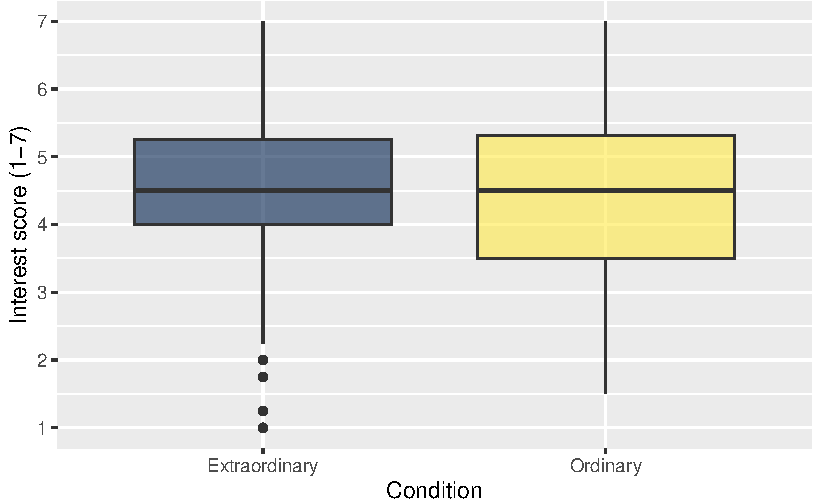
\includegraphics[width=1\textwidth,height=\textheight]{07-more-visualisation_files/figure-pdf/unnamed-chunk-12-1.pdf}
\end{center}

\end{tcolorbox}

\subsection{Activity 10 - Ordering
categories}\label{activity-10---ordering-categories}

When we plot variables like \texttt{Gender} on the x-axis, R has an
internal order it sets unless you create a factor. The default is
alphabetical or numerical. In previous plots, it displayed Female then
Male, as F comes before M.

Controlling the order of categories is an important design choice to
communicate your message, and the most direct way is controlling the
factor order before plotting. Here, we add \texttt{mutate()} in a pipe
and manually set the factor levels, just be careful as it is case
sensitive to the values in your data.

\begin{Shaded}
\begin{Highlighting}[]
\NormalTok{zhang\_data\_long }\SpecialCharTok{\%\textgreater{}\%} 
  \FunctionTok{drop\_na}\NormalTok{(Gender) }\SpecialCharTok{\%\textgreater{}\%} 
  \FunctionTok{mutate}\NormalTok{(}\AttributeTok{Gender =} \FunctionTok{factor}\NormalTok{(Gender, }
                         \AttributeTok{levels =} \FunctionTok{c}\NormalTok{(}\StringTok{"Male"}\NormalTok{, }\StringTok{"Female"}\NormalTok{))) }\SpecialCharTok{\%\textgreater{}\%} 
  \FunctionTok{ggplot}\NormalTok{(}\FunctionTok{aes}\NormalTok{(}\AttributeTok{y =}\NormalTok{ Interest, }\AttributeTok{x =}\NormalTok{ Gender, }\AttributeTok{fill =}\NormalTok{ Gender)) }\SpecialCharTok{+}
  \FunctionTok{geom\_boxplot}\NormalTok{() }\SpecialCharTok{+} 
  \FunctionTok{scale\_y\_continuous}\NormalTok{(}\AttributeTok{name =} \StringTok{"Interest score (1{-}7)"}\NormalTok{, }
                     \AttributeTok{breaks =} \FunctionTok{c}\NormalTok{(}\DecValTok{1}\SpecialCharTok{:}\DecValTok{7}\NormalTok{)) }\SpecialCharTok{+} 
  \FunctionTok{scale\_fill\_viridis\_d}\NormalTok{(}\AttributeTok{option =} \StringTok{"E"}\NormalTok{, }
                       \AttributeTok{alpha =} \FloatTok{0.6}\NormalTok{) }\SpecialCharTok{+} 
  \FunctionTok{guides}\NormalTok{(}\AttributeTok{fill =} \StringTok{"none"}\NormalTok{)}
\end{Highlighting}
\end{Shaded}

\begin{center}
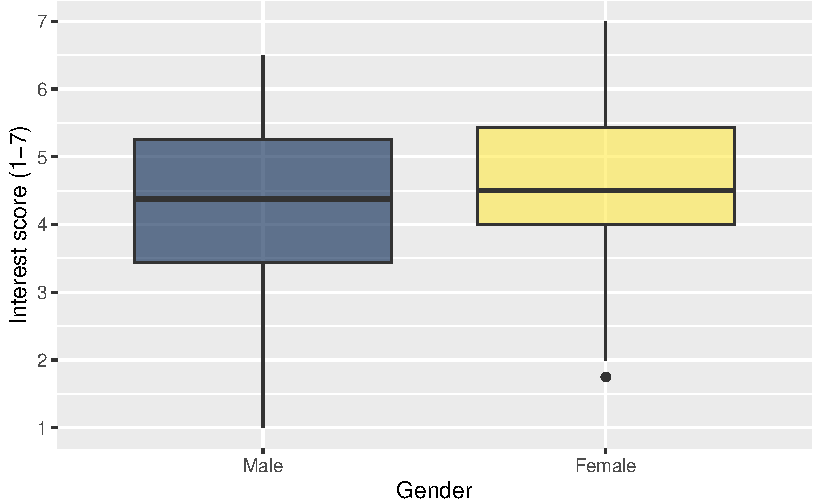
\includegraphics[width=1\textwidth,height=\textheight]{07-more-visualisation_files/figure-pdf/unnamed-chunk-13-1.pdf}
\end{center}

\subsection{Activity 11- Boxplots for multiple
factors}\label{activity-11--boxplots-for-multiple-factors}

When you only have one independent variable, using the \texttt{fill}
argument to change the colour can be a little redundant as the colours
do not add any additional information. It makes more sense to use colour
to represent a second variable.

For this example, we will use \texttt{Condition} and \texttt{Time} as
variables. \texttt{fill()} now specifies a second independent variable,
rather than repeating the variable on the x-axis as in the previous
plot, so we do not want to deactivate the legend.

\begin{Shaded}
\begin{Highlighting}[]
\NormalTok{zhang\_data\_long }\SpecialCharTok{\%\textgreater{}\%} 
  \FunctionTok{ggplot}\NormalTok{(}\FunctionTok{aes}\NormalTok{(}\AttributeTok{y =}\NormalTok{ Interest, }\AttributeTok{x =}\NormalTok{ Condition, }\AttributeTok{fill =}\NormalTok{ Time)) }\SpecialCharTok{+}
  \FunctionTok{geom\_boxplot}\NormalTok{() }\SpecialCharTok{+} 
  \FunctionTok{scale\_y\_continuous}\NormalTok{(}\AttributeTok{name =} \StringTok{"Interest score (1{-}7)"}\NormalTok{, }
                     \AttributeTok{breaks =} \FunctionTok{c}\NormalTok{(}\DecValTok{1}\SpecialCharTok{:}\DecValTok{7}\NormalTok{)) }\SpecialCharTok{+} 
  \FunctionTok{scale\_fill\_viridis\_d}\NormalTok{(}\AttributeTok{option =} \StringTok{"E"}\NormalTok{, }
                       \AttributeTok{alpha =} \FloatTok{0.6}\NormalTok{)}
\end{Highlighting}
\end{Shaded}

\begin{center}
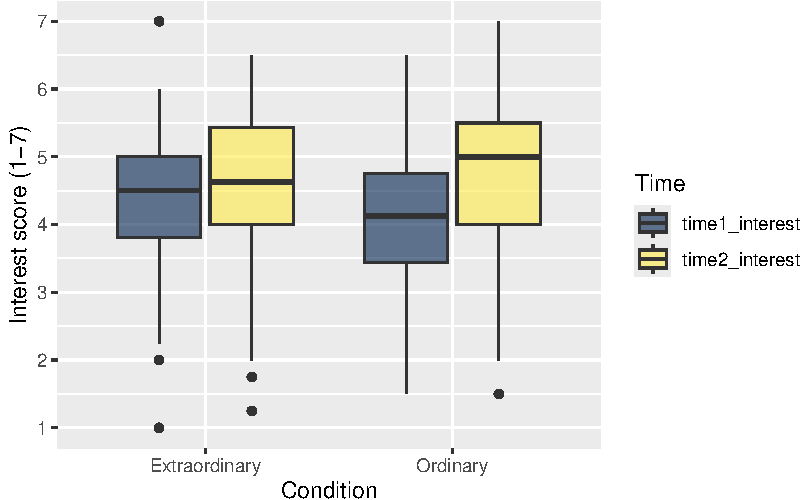
\includegraphics[width=1\textwidth,height=\textheight]{07-more-visualisation_files/figure-pdf/bp5-1.pdf}
\end{center}

As a final point here, the \texttt{fill} values on the legend are not
the most professional looking. Like reordering factors, the easiest way
of addressing this is editing the underlying data before piping to
ggplot2.

\begin{Shaded}
\begin{Highlighting}[]
\NormalTok{zhang\_data\_long }\SpecialCharTok{\%\textgreater{}\%} 
  \FunctionTok{mutate}\NormalTok{(}\AttributeTok{Time =} \FunctionTok{case\_match}\NormalTok{(Time,}
                           \StringTok{"time1\_interest"} \SpecialCharTok{\textasciitilde{}} \StringTok{"Time 1"}\NormalTok{,}
                           \StringTok{"time2\_interest"} \SpecialCharTok{\textasciitilde{}} \StringTok{"Time 2"}\NormalTok{)) }\SpecialCharTok{\%\textgreater{}\%} 
  \FunctionTok{ggplot}\NormalTok{(}\FunctionTok{aes}\NormalTok{(}\AttributeTok{y =}\NormalTok{ Interest, }\AttributeTok{x =}\NormalTok{ Condition, }\AttributeTok{fill =}\NormalTok{ Time)) }\SpecialCharTok{+}
  \FunctionTok{geom\_boxplot}\NormalTok{() }\SpecialCharTok{+} 
  \FunctionTok{scale\_y\_continuous}\NormalTok{(}\AttributeTok{name =} \StringTok{"Interest score (1{-}7)"}\NormalTok{, }
                     \AttributeTok{breaks =} \FunctionTok{c}\NormalTok{(}\DecValTok{1}\SpecialCharTok{:}\DecValTok{7}\NormalTok{)) }\SpecialCharTok{+} 
  \FunctionTok{scale\_fill\_viridis\_d}\NormalTok{(}\AttributeTok{option =} \StringTok{"E"}\NormalTok{, }
                       \AttributeTok{alpha =} \FloatTok{0.6}\NormalTok{)}
\end{Highlighting}
\end{Shaded}

\begin{center}
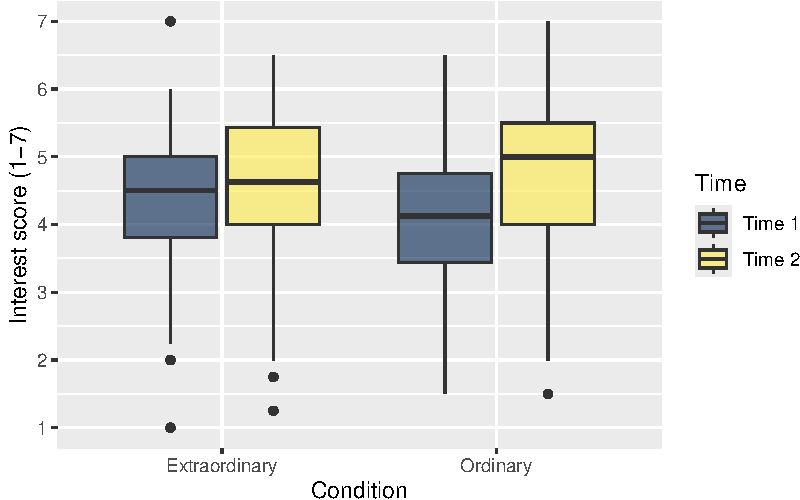
\includegraphics[width=1\textwidth,height=\textheight]{07-more-visualisation_files/figure-pdf/unnamed-chunk-14-1.pdf}
\end{center}

\section{Violin-boxplots}\label{viz-a7}

Boxplots are great for your own exploratory data analysis but you do not
often see them reported in isolation. They visualise summary statistics,
but you do not get much sense of the underlying distribution of values.
When you want to communicate continuous outcomes, researchers in
psychology are using violin-boxplots more often. This combines both
elements: a violin plot to show the distribution of the data, and a
boxplot to add summary statistics. This is where ggplot2 comes into it's
own as we can add and customise several layers.

\subsection{Activity 12 - Creating a basic violin
plot}\label{activity-12---creating-a-basic-violin-plot}

Violin plots get their name as they look something like a violin when
the data are roughly normally distributed. They show density, so the
fatter the violin element, the more data points there are for that
value. Compared to the boxplot, the only difference is changing the
layer to \texttt{geom\_violin()}.

\begin{Shaded}
\begin{Highlighting}[]
\NormalTok{zhang\_data\_long }\SpecialCharTok{\%\textgreater{}\%} 
  \FunctionTok{drop\_na}\NormalTok{(Gender) }\SpecialCharTok{\%\textgreater{}\%} 
  \FunctionTok{ggplot}\NormalTok{(}\FunctionTok{aes}\NormalTok{(}\AttributeTok{y =}\NormalTok{ Interest, }\AttributeTok{x =}\NormalTok{ Gender)) }\SpecialCharTok{+}
  \FunctionTok{geom\_violin}\NormalTok{() }\SpecialCharTok{+} 
  \FunctionTok{scale\_y\_continuous}\NormalTok{(}\AttributeTok{name =} \StringTok{"Interest score (1{-}7)"}\NormalTok{, }
                     \AttributeTok{breaks =} \FunctionTok{c}\NormalTok{(}\DecValTok{1}\SpecialCharTok{:}\DecValTok{7}\NormalTok{))}
\end{Highlighting}
\end{Shaded}

\begin{center}
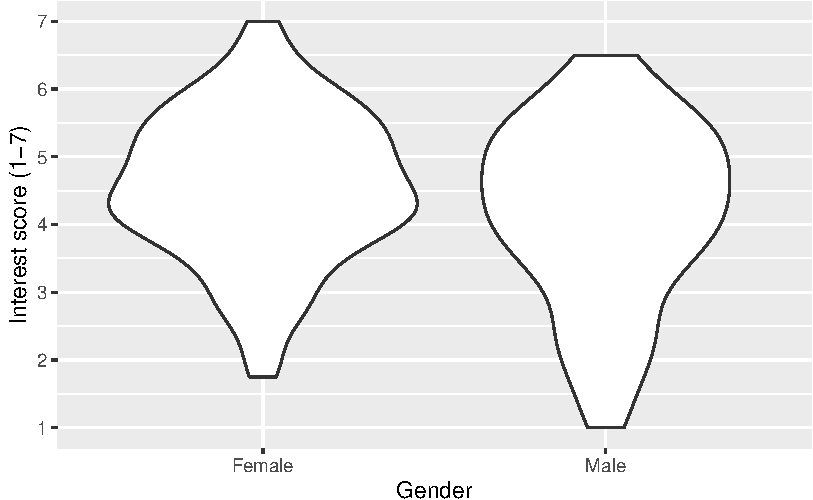
\includegraphics[width=1\textwidth,height=\textheight]{07-more-visualisation_files/figure-pdf/vp1-1.pdf}
\end{center}

The distribution of values is great, but sometimes it might be useful to
also add the underlying data points. These are all important design
choices as it can be useful when you have smaller amounts of data, but
overwhelming when you have thousands of data points. So, keep in mind
what you want to communicate. Here, we use the layer
\texttt{geom\_jitter()} to jitter the points slightly, so they are not
all in a vertical line and we get a better sense of the density.

\begin{Shaded}
\begin{Highlighting}[]
\NormalTok{zhang\_data\_long }\SpecialCharTok{\%\textgreater{}\%} 
  \FunctionTok{drop\_na}\NormalTok{(Gender) }\SpecialCharTok{\%\textgreater{}\%} 
  \FunctionTok{ggplot}\NormalTok{(}\FunctionTok{aes}\NormalTok{(}\AttributeTok{y =}\NormalTok{ Interest, }\AttributeTok{x =}\NormalTok{ Gender)) }\SpecialCharTok{+}
  \FunctionTok{geom\_violin}\NormalTok{() }\SpecialCharTok{+} 
  \FunctionTok{geom\_jitter}\NormalTok{(}\AttributeTok{height =} \DecValTok{0}\NormalTok{, }\CommentTok{\# do not jitter height}
              \AttributeTok{width =}\NormalTok{ .}\DecValTok{1}\NormalTok{) }\SpecialCharTok{+} \CommentTok{\# jitter width of points}
  \FunctionTok{scale\_y\_continuous}\NormalTok{(}\AttributeTok{name =} \StringTok{"Interest score (1{-}7)"}\NormalTok{, }
                     \AttributeTok{breaks =} \FunctionTok{c}\NormalTok{(}\DecValTok{1}\SpecialCharTok{:}\DecValTok{7}\NormalTok{))}
\end{Highlighting}
\end{Shaded}

\begin{center}
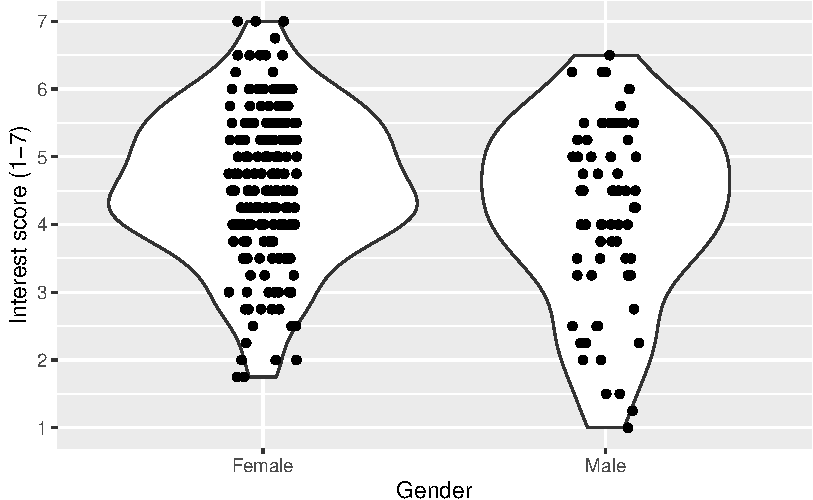
\includegraphics[width=1\textwidth,height=\textheight]{07-more-visualisation_files/figure-pdf/vp2-1.pdf}
\end{center}

\begin{tcolorbox}[enhanced jigsaw, breakable, colframe=quarto-callout-important-color-frame, arc=.35mm, opacitybacktitle=0.6, titlerule=0mm, colbacktitle=quarto-callout-important-color!10!white, colback=white, toprule=.15mm, bottomtitle=1mm, toptitle=1mm, title=\textcolor{quarto-callout-important-color}{\faExclamation}\hspace{0.5em}{Important}, bottomrule=.15mm, rightrule=.15mm, leftrule=.75mm, coltitle=black, left=2mm, opacityback=0]

It is important to remember that R is very literal. ggplot2 works on a
system of layers. It will add new geoms on top of existing ones and it
will not stop to think whether this is a good idea. Try running the code
above but put \texttt{geom\_jitter()} first and then add
\texttt{geom\_violin()}. The order of your layers matters.

\end{tcolorbox}

\subsection{Activity 13 - Creating a
violin-boxplot}\label{activity-13---creating-a-violin-boxplot}

Instead of adding the data points in a layer, we can add a boxplot to
create the violin-boxplot. This way, we get distribution information
from the violin layer and summary statistics from the boxplot layer.

\begin{Shaded}
\begin{Highlighting}[]
\NormalTok{zhang\_data\_long }\SpecialCharTok{\%\textgreater{}\%} 
  \FunctionTok{drop\_na}\NormalTok{(Gender) }\SpecialCharTok{\%\textgreater{}\%} 
  \FunctionTok{ggplot}\NormalTok{(}\FunctionTok{aes}\NormalTok{(}\AttributeTok{y =}\NormalTok{ Interest, }\AttributeTok{x =}\NormalTok{ Gender)) }\SpecialCharTok{+}
  \FunctionTok{geom\_violin}\NormalTok{() }\SpecialCharTok{+} 
  \FunctionTok{geom\_boxplot}\NormalTok{() }\SpecialCharTok{+} 
  \FunctionTok{scale\_y\_continuous}\NormalTok{(}\AttributeTok{name =} \StringTok{"Interest score (1{-}7)"}\NormalTok{, }
                     \AttributeTok{breaks =} \FunctionTok{c}\NormalTok{(}\DecValTok{1}\SpecialCharTok{:}\DecValTok{7}\NormalTok{))}
\end{Highlighting}
\end{Shaded}

\begin{center}
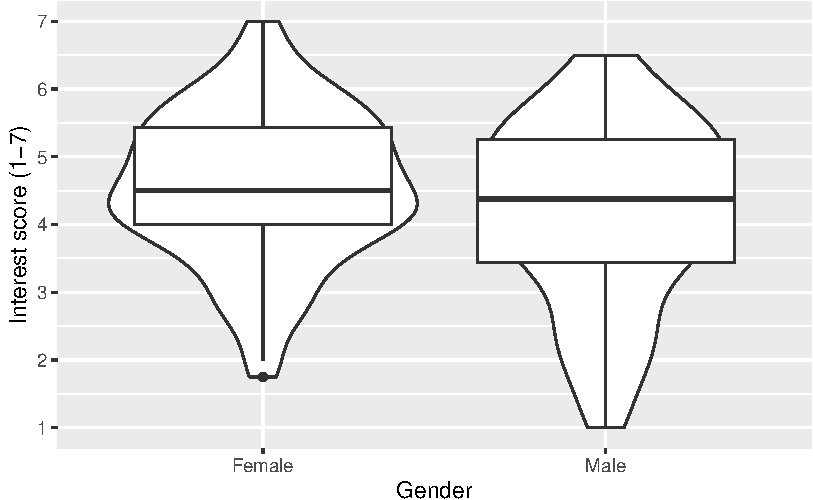
\includegraphics[width=1\textwidth,height=\textheight]{07-more-visualisation_files/figure-pdf/unnamed-chunk-15-1.pdf}
\end{center}

On it's own, this does not look great. We can edit the settings to
reduce the width of the boxplots, add a colour scheme, and add
transparency to the violin layer to make it easier to see the boxplot.

\begin{Shaded}
\begin{Highlighting}[]
\NormalTok{zhang\_data\_long }\SpecialCharTok{\%\textgreater{}\%} 
  \FunctionTok{drop\_na}\NormalTok{(Gender) }\SpecialCharTok{\%\textgreater{}\%} 
  \FunctionTok{ggplot}\NormalTok{(}\FunctionTok{aes}\NormalTok{(}\AttributeTok{y =}\NormalTok{ Interest, }\AttributeTok{x =}\NormalTok{ Gender, }\AttributeTok{fill =}\NormalTok{ Gender)) }\SpecialCharTok{+}
  \FunctionTok{geom\_violin}\NormalTok{(}\AttributeTok{alpha =} \FloatTok{0.5}\NormalTok{) }\SpecialCharTok{+} 
  \FunctionTok{geom\_boxplot}\NormalTok{(}\AttributeTok{width =} \FloatTok{0.2}\NormalTok{) }\SpecialCharTok{+} 
  \FunctionTok{scale\_fill\_viridis\_d}\NormalTok{(}\AttributeTok{option =} \StringTok{"E"}\NormalTok{) }\SpecialCharTok{+} 
  \FunctionTok{scale\_y\_continuous}\NormalTok{(}\AttributeTok{name =} \StringTok{"Interest score (1{-}7)"}\NormalTok{, }
                     \AttributeTok{breaks =} \FunctionTok{c}\NormalTok{(}\DecValTok{1}\SpecialCharTok{:}\DecValTok{7}\NormalTok{)) }\SpecialCharTok{+} 
  \FunctionTok{guides}\NormalTok{(}\AttributeTok{fill =} \StringTok{"none"}\NormalTok{)}
\end{Highlighting}
\end{Shaded}

\begin{center}
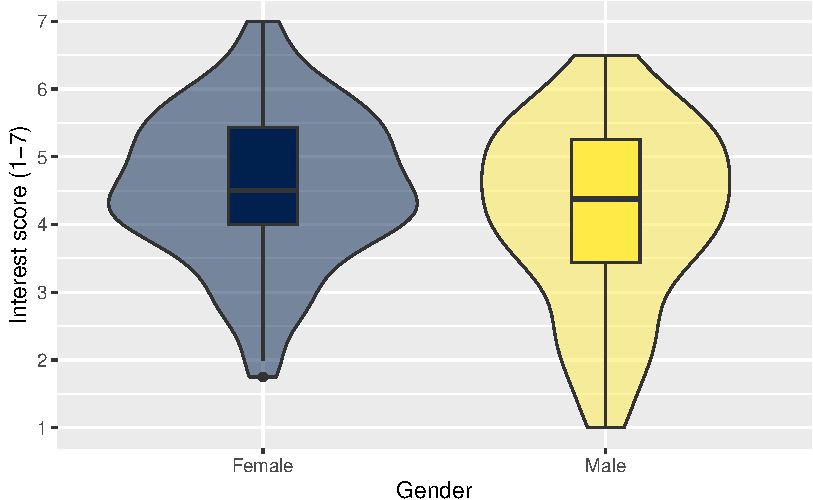
\includegraphics[width=1\textwidth,height=\textheight]{07-more-visualisation_files/figure-pdf/unnamed-chunk-16-1.pdf}
\end{center}

The boxplot uses the median for the centre line, but in your report you
might be presenting means per category which will be slightly different.
One further variation is removing the centre median line, and replacing
it with the mean and 95\% confidence interval (more on that in the
lectures and Chapter 8). This way, you get three layers: the violin plot
for the density, the boxplot for distribution summary statistics, and
the mean and 95\% confidence interval.

This code uses two calls to \texttt{stat\_summary()} which is a layer to
add summary statistics. The first layer draws a \texttt{point} to
represent the mean, and the second draws an \texttt{errorbar} that
represents the 95\% confidence interval around the mean.

\begin{Shaded}
\begin{Highlighting}[]
\NormalTok{zhang\_data\_long }\SpecialCharTok{\%\textgreater{}\%} 
  \FunctionTok{drop\_na}\NormalTok{(Gender) }\SpecialCharTok{\%\textgreater{}\%} 
  \FunctionTok{ggplot}\NormalTok{(}\FunctionTok{aes}\NormalTok{(}\AttributeTok{y =}\NormalTok{ Interest, }\AttributeTok{x =}\NormalTok{ Gender, }\AttributeTok{fill =}\NormalTok{ Gender)) }\SpecialCharTok{+}
  \FunctionTok{geom\_violin}\NormalTok{(}\AttributeTok{alpha =} \FloatTok{0.5}\NormalTok{) }\SpecialCharTok{+} 
  \FunctionTok{geom\_boxplot}\NormalTok{(}\AttributeTok{width =} \FloatTok{0.2}\NormalTok{, }
               \AttributeTok{fatten =} \ConstantTok{NULL}\NormalTok{) }\SpecialCharTok{+} 
  \FunctionTok{stat\_summary}\NormalTok{(}\AttributeTok{fun =} \StringTok{"mean"}\NormalTok{, }
               \AttributeTok{geom =} \StringTok{"point"}\NormalTok{) }\SpecialCharTok{+}
  \FunctionTok{stat\_summary}\NormalTok{(}\AttributeTok{fun.data =} \StringTok{"mean\_cl\_boot"}\NormalTok{, }\CommentTok{\# confidence interval}
               \AttributeTok{geom =} \StringTok{"errorbar"}\NormalTok{, }
               \AttributeTok{width =} \FloatTok{0.1}\NormalTok{) }\SpecialCharTok{+}
  \FunctionTok{scale\_fill\_viridis\_d}\NormalTok{(}\AttributeTok{option =} \StringTok{"E"}\NormalTok{) }\SpecialCharTok{+} 
  \FunctionTok{scale\_y\_continuous}\NormalTok{(}\AttributeTok{name =} \StringTok{"Interest score (1{-}7)"}\NormalTok{, }
                     \AttributeTok{breaks =} \FunctionTok{c}\NormalTok{(}\DecValTok{1}\SpecialCharTok{:}\DecValTok{7}\NormalTok{)) }\SpecialCharTok{+} 
  \FunctionTok{guides}\NormalTok{(}\AttributeTok{fill =} \StringTok{"none"}\NormalTok{)}
\end{Highlighting}
\end{Shaded}

\begin{center}
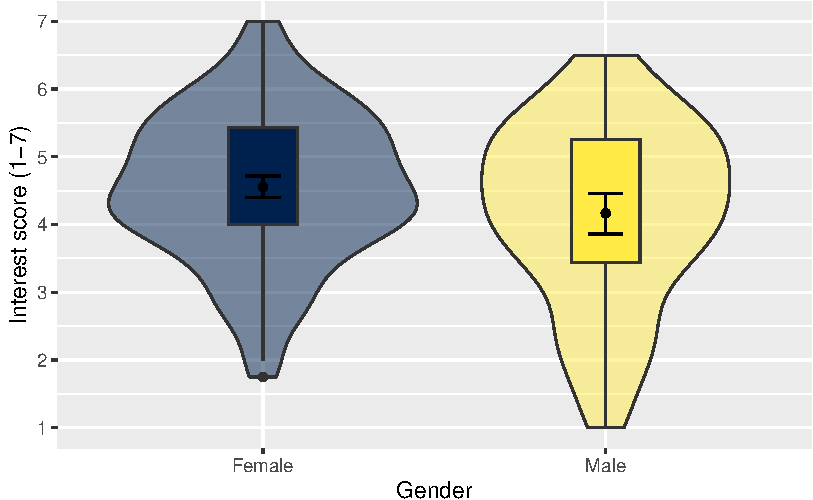
\includegraphics[width=1\textwidth,height=\textheight]{07-more-visualisation_files/figure-pdf/vbp1-1.pdf}
\end{center}

\begin{tcolorbox}[enhanced jigsaw, breakable, colframe=quarto-callout-warning-color-frame, arc=.35mm, opacitybacktitle=0.6, titlerule=0mm, colbacktitle=quarto-callout-warning-color!10!white, colback=white, toprule=.15mm, bottomtitle=1mm, toptitle=1mm, title=\textcolor{quarto-callout-warning-color}{\faExclamationTriangle}\hspace{0.5em}{Warning}, bottomrule=.15mm, rightrule=.15mm, leftrule=.75mm, coltitle=black, left=2mm, opacityback=0]

When you run the line
\texttt{stat\_summary(fun.data\ =\ "mean\_cl\_boot",\ geom\ =\ "errorbar",\ width\ =\ .1)}
for the first time, you might be prompted to install the R package
Hmisc. If you are on your own computer, follow the instructions in the
Console to install the package. If you are on a university computer,
this should already be installed.

\end{tcolorbox}

\begin{tcolorbox}[enhanced jigsaw, breakable, colframe=quarto-callout-tip-color-frame, arc=.35mm, opacitybacktitle=0.6, titlerule=0mm, colbacktitle=quarto-callout-tip-color!10!white, colback=white, toprule=.15mm, bottomtitle=1mm, toptitle=1mm, title=\textcolor{quarto-callout-tip-color}{\faLightbulb}\hspace{0.5em}{Try this}, bottomrule=.15mm, rightrule=.15mm, leftrule=.75mm, coltitle=black, left=2mm, opacityback=0]

For your independent violin-boxplot, use \texttt{zhang\_data\_long} to
visualise \texttt{Interest} as your continuous variable and
\texttt{Condition} for different categories on the x-axis. Try and
create the plot to look like this, so you might need to play around with
different themes:

\begin{center}
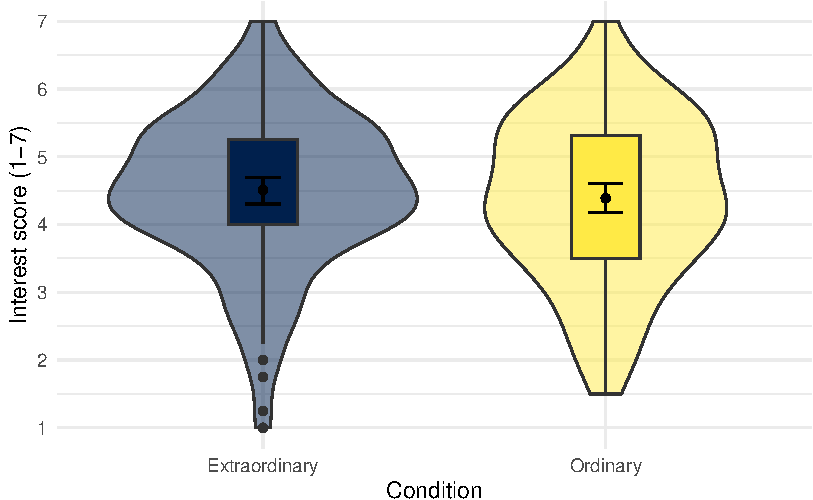
\includegraphics[width=1\textwidth,height=\textheight]{07-more-visualisation_files/figure-pdf/unnamed-chunk-17-1.pdf}
\end{center}

\end{tcolorbox}

\begin{tcolorbox}[enhanced jigsaw, breakable, colframe=quarto-callout-caution-color-frame, arc=.35mm, opacitybacktitle=0.6, titlerule=0mm, colbacktitle=quarto-callout-caution-color!10!white, colback=white, toprule=.15mm, bottomtitle=1mm, toptitle=1mm, title=\textcolor{quarto-callout-caution-color}{\faFire}\hspace{0.5em}{Show me the solution}, bottomrule=.15mm, rightrule=.15mm, leftrule=.75mm, coltitle=black, left=2mm, opacityback=0]

You should have the following in a code chunk:

\begin{Shaded}
\begin{Highlighting}[]
\NormalTok{zhang\_data\_long }\SpecialCharTok{\%\textgreater{}\%} 
  \FunctionTok{ggplot}\NormalTok{(}\FunctionTok{aes}\NormalTok{(}\AttributeTok{y =}\NormalTok{ Interest, }\AttributeTok{x =}\NormalTok{ Condition, }\AttributeTok{fill =}\NormalTok{ Condition)) }\SpecialCharTok{+}
  \FunctionTok{geom\_violin}\NormalTok{(}\AttributeTok{alpha =} \FloatTok{0.5}\NormalTok{) }\SpecialCharTok{+} 
  \FunctionTok{geom\_boxplot}\NormalTok{(}\AttributeTok{width =} \FloatTok{0.2}\NormalTok{, }
               \AttributeTok{fatten =} \ConstantTok{NULL}\NormalTok{) }\SpecialCharTok{+} 
  \FunctionTok{stat\_summary}\NormalTok{(}\AttributeTok{fun =} \StringTok{"mean"}\NormalTok{, }
               \AttributeTok{geom =} \StringTok{"point"}\NormalTok{) }\SpecialCharTok{+}
  \FunctionTok{stat\_summary}\NormalTok{(}\AttributeTok{fun.data =} \StringTok{"mean\_cl\_boot"}\NormalTok{, }
               \AttributeTok{geom =} \StringTok{"errorbar"}\NormalTok{, }
               \AttributeTok{width =}\NormalTok{ .}\DecValTok{1}\NormalTok{) }\SpecialCharTok{+}
  \FunctionTok{scale\_fill\_viridis\_d}\NormalTok{(}\AttributeTok{option =} \StringTok{"E"}\NormalTok{) }\SpecialCharTok{+} 
  \FunctionTok{scale\_y\_continuous}\NormalTok{(}\AttributeTok{name =} \StringTok{"Interest score (1{-}7)"}\NormalTok{, }
                     \AttributeTok{breaks =} \FunctionTok{c}\NormalTok{(}\DecValTok{1}\SpecialCharTok{:}\DecValTok{7}\NormalTok{)) }\SpecialCharTok{+} 
  \FunctionTok{theme\_minimal}\NormalTok{() }\SpecialCharTok{+} 
  \FunctionTok{guides}\NormalTok{(}\AttributeTok{fill =} \StringTok{"none"}\NormalTok{)}
\end{Highlighting}
\end{Shaded}

\end{tcolorbox}

\subsection{Activity 14 - Adding additional
variables}\label{activity-14---adding-additional-variables}

Like boxplots, we can add a second grouping variable to \texttt{fill}
instead of just using it for colour.

\begin{Shaded}
\begin{Highlighting}[]
\NormalTok{zhang\_data\_long }\SpecialCharTok{\%\textgreater{}\%} 
  \FunctionTok{ggplot}\NormalTok{(}\FunctionTok{aes}\NormalTok{(}\AttributeTok{y =}\NormalTok{ Interest, }\AttributeTok{x =}\NormalTok{ Condition, }\AttributeTok{fill =}\NormalTok{ Time)) }\SpecialCharTok{+}
  \FunctionTok{geom\_violin}\NormalTok{(}\AttributeTok{alpha =} \FloatTok{0.5}\NormalTok{) }\SpecialCharTok{+} 
  \FunctionTok{geom\_boxplot}\NormalTok{(}\AttributeTok{width =} \FloatTok{0.2}\NormalTok{, }
               \AttributeTok{fatten =} \ConstantTok{NULL}\NormalTok{) }\SpecialCharTok{+} 
  \FunctionTok{stat\_summary}\NormalTok{(}\AttributeTok{fun =} \StringTok{"mean"}\NormalTok{, }
               \AttributeTok{geom =} \StringTok{"point"}\NormalTok{) }\SpecialCharTok{+}
  \FunctionTok{stat\_summary}\NormalTok{(}\AttributeTok{fun.data =} \StringTok{"mean\_cl\_boot"}\NormalTok{, }
               \AttributeTok{geom =} \StringTok{"errorbar"}\NormalTok{, }
               \AttributeTok{width =}\NormalTok{ .}\DecValTok{1}\NormalTok{) }\SpecialCharTok{+}
  \FunctionTok{scale\_fill\_viridis\_d}\NormalTok{(}\AttributeTok{option =} \StringTok{"E"}\NormalTok{) }\SpecialCharTok{+} 
  \FunctionTok{scale\_y\_continuous}\NormalTok{(}\AttributeTok{name =} \StringTok{"Interest score (1{-}7)"}\NormalTok{, }
                     \AttributeTok{breaks =} \FunctionTok{c}\NormalTok{(}\DecValTok{1}\SpecialCharTok{:}\DecValTok{7}\NormalTok{)) }\SpecialCharTok{+} 
  \FunctionTok{theme\_minimal}\NormalTok{()}
\end{Highlighting}
\end{Shaded}

\begin{center}
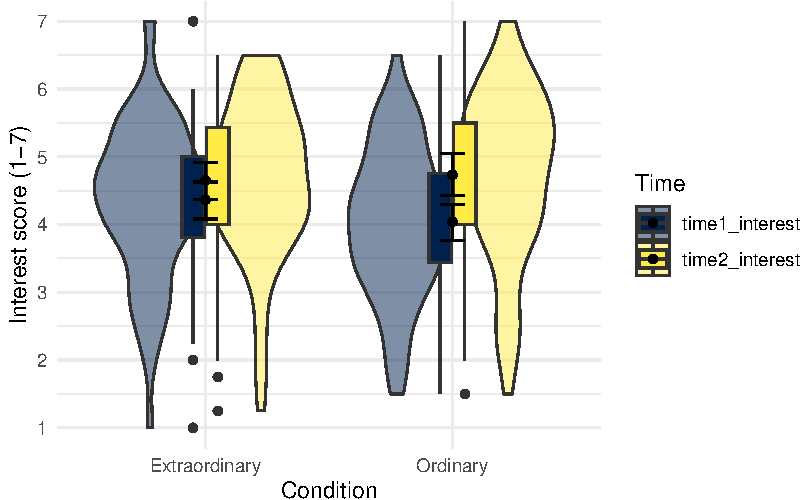
\includegraphics[width=1\textwidth,height=\textheight]{07-more-visualisation_files/figure-pdf/unnamed-chunk-19-1.pdf}
\end{center}

However, unless you are trying to recreate a Kandinsky painting in
ggplot2, that does not look quite right. This is because we have
multiple layers that each plot separate groups in different ways. To
make it all fall into line, we need to add a constant value to offset
the elements. We start off by defining a position dodge value as an
object. This way, we can use the object name later, and we only need to
edit it in one place if we wanted to change the value.

\begin{Shaded}
\begin{Highlighting}[]
\CommentTok{\# specify as an object, so we only change it in one place}
\NormalTok{dodge\_value }\OtherTok{\textless{}{-}} \FloatTok{0.9}

\NormalTok{zhang\_data\_long }\SpecialCharTok{\%\textgreater{}\%} 
  \FunctionTok{ggplot}\NormalTok{(}\FunctionTok{aes}\NormalTok{(}\AttributeTok{y =}\NormalTok{ Interest, }\AttributeTok{x =}\NormalTok{ Condition, }\AttributeTok{fill =}\NormalTok{ Time)) }\SpecialCharTok{+}
  \FunctionTok{geom\_violin}\NormalTok{(}\AttributeTok{alpha =} \FloatTok{0.5}\NormalTok{) }\SpecialCharTok{+} 
  \FunctionTok{geom\_boxplot}\NormalTok{(}\AttributeTok{width =} \FloatTok{0.2}\NormalTok{, }
               \AttributeTok{fatten =} \ConstantTok{NULL}\NormalTok{,}
               \AttributeTok{position =} \FunctionTok{position\_dodge}\NormalTok{(dodge\_value)) }\SpecialCharTok{+} 
  \FunctionTok{stat\_summary}\NormalTok{(}\AttributeTok{fun =} \StringTok{"mean"}\NormalTok{, }
               \AttributeTok{geom =} \StringTok{"point"}\NormalTok{,}
               \AttributeTok{position =} \FunctionTok{position\_dodge}\NormalTok{(dodge\_value)) }\SpecialCharTok{+}
  \FunctionTok{stat\_summary}\NormalTok{(}\AttributeTok{fun.data =} \StringTok{"mean\_cl\_boot"}\NormalTok{, }
               \AttributeTok{geom =} \StringTok{"errorbar"}\NormalTok{, }
               \AttributeTok{width =}\NormalTok{ .}\DecValTok{1}\NormalTok{,}
               \AttributeTok{position =} \FunctionTok{position\_dodge}\NormalTok{(dodge\_value)) }\SpecialCharTok{+}
  \FunctionTok{scale\_fill\_viridis\_d}\NormalTok{(}\AttributeTok{option =} \StringTok{"E"}\NormalTok{) }\SpecialCharTok{+} 
  \FunctionTok{scale\_y\_continuous}\NormalTok{(}\AttributeTok{name =} \StringTok{"Interest score (1{-}7)"}\NormalTok{, }
                     \AttributeTok{breaks =} \FunctionTok{c}\NormalTok{(}\DecValTok{1}\SpecialCharTok{:}\DecValTok{7}\NormalTok{))}
\end{Highlighting}
\end{Shaded}

\begin{center}
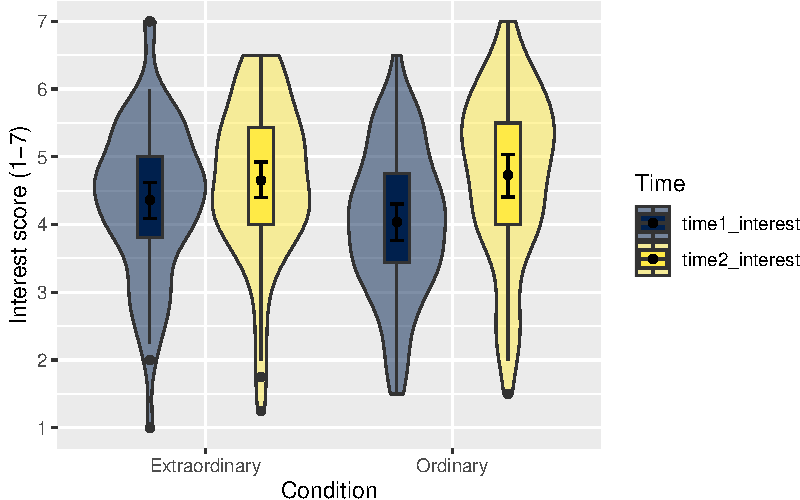
\includegraphics[width=1\textwidth,height=\textheight]{07-more-visualisation_files/figure-pdf/unnamed-chunk-20-1.pdf}
\end{center}

This looks much better! Remember, if you want to change the legend
labels, the easiest way is recoding the data before piping to ggplot2.

Finally, we might want to add a third variable to group the data by.
There is a facet function that produces different plots for each level
of a grouping variable which can be very useful when you have more than
two factors. The following code shows interest ratings for all three
variables we have worked with: Condition, Time, and Gender.

\begin{Shaded}
\begin{Highlighting}[]
\CommentTok{\# specify as an object, so we only change it in one place}
\NormalTok{dodge\_value }\OtherTok{\textless{}{-}} \FloatTok{0.9}

\NormalTok{zhang\_data\_long }\SpecialCharTok{\%\textgreater{}\%} 
  \FunctionTok{drop\_na}\NormalTok{(Gender) }\SpecialCharTok{\%\textgreater{}\%} 
  \FunctionTok{ggplot}\NormalTok{(}\FunctionTok{aes}\NormalTok{(}\AttributeTok{y =}\NormalTok{ Interest, }\AttributeTok{x =}\NormalTok{ Condition, }\AttributeTok{fill =}\NormalTok{ Time)) }\SpecialCharTok{+}
  \FunctionTok{geom\_violin}\NormalTok{(}\AttributeTok{alpha =} \FloatTok{0.5}\NormalTok{) }\SpecialCharTok{+} 
  \FunctionTok{geom\_boxplot}\NormalTok{(}\AttributeTok{width =} \FloatTok{0.2}\NormalTok{, }
               \AttributeTok{fatten =} \ConstantTok{NULL}\NormalTok{,}
               \AttributeTok{position =} \FunctionTok{position\_dodge}\NormalTok{(dodge\_value)) }\SpecialCharTok{+} 
  \FunctionTok{stat\_summary}\NormalTok{(}\AttributeTok{fun =} \StringTok{"mean"}\NormalTok{, }
               \AttributeTok{geom =} \StringTok{"point"}\NormalTok{,}
               \AttributeTok{position =} \FunctionTok{position\_dodge}\NormalTok{(dodge\_value)) }\SpecialCharTok{+}
  \FunctionTok{stat\_summary}\NormalTok{(}\AttributeTok{fun.data =} \StringTok{"mean\_cl\_boot"}\NormalTok{, }
               \AttributeTok{geom =} \StringTok{"errorbar"}\NormalTok{, }
               \AttributeTok{width =}\NormalTok{ .}\DecValTok{1}\NormalTok{,}
               \AttributeTok{position =} \FunctionTok{position\_dodge}\NormalTok{(dodge\_value)) }\SpecialCharTok{+}
  \FunctionTok{facet\_wrap}\NormalTok{(}\SpecialCharTok{\textasciitilde{}}\NormalTok{ Gender) }\SpecialCharTok{+} \CommentTok{\# facet by Gender}
  \FunctionTok{scale\_fill\_viridis\_d}\NormalTok{(}\AttributeTok{option =} \StringTok{"E"}\NormalTok{) }\SpecialCharTok{+} 
  \FunctionTok{scale\_y\_continuous}\NormalTok{(}\AttributeTok{name =} \StringTok{"Interest score (1{-}7)"}\NormalTok{, }
                     \AttributeTok{breaks =} \FunctionTok{c}\NormalTok{(}\DecValTok{1}\SpecialCharTok{:}\DecValTok{7}\NormalTok{))}
\end{Highlighting}
\end{Shaded}

\begin{center}
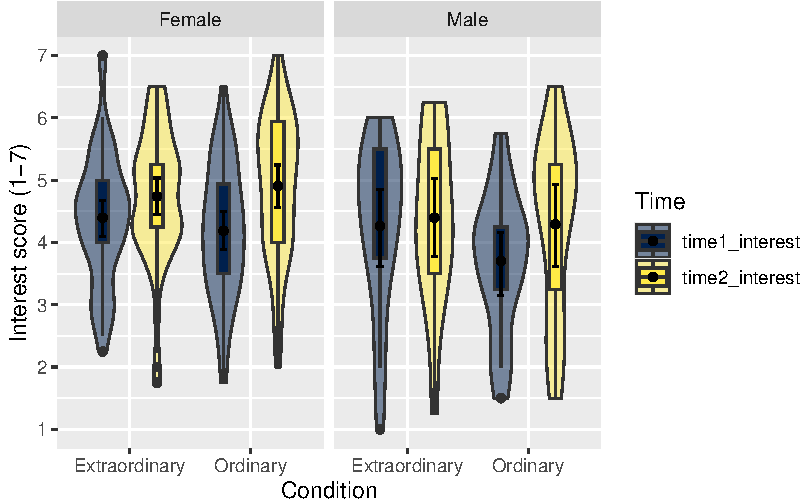
\includegraphics[width=1\textwidth,height=\textheight]{07-more-visualisation_files/figure-pdf/facet1-1.pdf}
\end{center}

Facets work in the same way as adding a variable to \texttt{fill}. It is
not easy to change the labels within ggplot2, you are better off editing
the values in your data first.

\section{Test yourself}\label{test-yourself-5}

To end the chapter, we have some knowledge check questions to test your
understanding of the concepts we covered in the chapter. We then have
some error mode tasks to see if you can find the solution to some common
errors in the concepts we covered in this chapter.

\subsection{Knowledge check}\label{knowledge-check-6}

\textbf{Question 1}. You want to plot several summary statistics
including the median for your outcome, which ggplot2 layer could you
use?

\begin{itemize}
\tightlist
\item
  \begin{enumerate}
  \def\labelenumi{(\Alph{enumi})}
  \tightlist
  \item
    geom\_boxplot()\\
  \end{enumerate}
\item
  \begin{enumerate}
  \def\labelenumi{(\Alph{enumi})}
  \setcounter{enumi}{1}
  \tightlist
  \item
    geom\_point()\\
  \end{enumerate}
\item
  \begin{enumerate}
  \def\labelenumi{(\Alph{enumi})}
  \setcounter{enumi}{2}
  \tightlist
  \item
    geom\_violin()
  \end{enumerate}
\end{itemize}

\textbf{Question 2}. You want to create a scatterplot to show the
correlation between two continuous variables, which ggplot2 layer could
you use?

\begin{itemize}
\tightlist
\item
  \begin{enumerate}
  \def\labelenumi{(\Alph{enumi})}
  \tightlist
  \item
    geom\_violin()\\
  \end{enumerate}
\item
  \begin{enumerate}
  \def\labelenumi{(\Alph{enumi})}
  \setcounter{enumi}{1}
  \tightlist
  \item
    geom\_point()\\
  \end{enumerate}
\item
  \begin{enumerate}
  \def\labelenumi{(\Alph{enumi})}
  \setcounter{enumi}{2}
  \tightlist
  \item
    geom\_boxplot()
  \end{enumerate}
\end{itemize}

\textbf{Question 3}. You want to show the density of values in your
outcome, which ggplot2 layer could you use?

\begin{itemize}
\tightlist
\item
  \begin{enumerate}
  \def\labelenumi{(\Alph{enumi})}
  \tightlist
  \item
    geom\_point()\\
  \end{enumerate}
\item
  \begin{enumerate}
  \def\labelenumi{(\Alph{enumi})}
  \setcounter{enumi}{1}
  \tightlist
  \item
    geom\_violin()\\
  \end{enumerate}
\item
  \begin{enumerate}
  \def\labelenumi{(\Alph{enumi})}
  \setcounter{enumi}{2}
  \tightlist
  \item
    geom\_boxplot()
  \end{enumerate}
\end{itemize}

\textbf{Question 4}. To separate a scatterplot into different groups,
you could specify a grouping variable using the \texttt{fill} argument
to change the colour of the points? TRUE / FALSE

\begin{tcolorbox}[enhanced jigsaw, breakable, colframe=quarto-callout-caution-color-frame, arc=.35mm, opacitybacktitle=0.6, titlerule=0mm, colbacktitle=quarto-callout-caution-color!10!white, colback=white, toprule=.15mm, bottomtitle=1mm, toptitle=1mm, title=\textcolor{quarto-callout-caution-color}{\faFire}\hspace{0.5em}{Explain this answer}, bottomrule=.15mm, rightrule=.15mm, leftrule=.75mm, coltitle=black, left=2mm, opacityback=0]

This was a sneaky one, but relates to the error mode warning within the
chapter. There are two ways to add a grouping variable for separate
colours: \texttt{colour} and \texttt{fill}. In this scenario,
\texttt{colour} would change the colour of the points, whereas
\texttt{fill} would only change the colour of the regression line and
its 95\% confidence interval ribbon. Sometimes you need to play around
with the settings to produce the effects you want.

\end{tcolorbox}

\textbf{Question 5}. The order of layers is important in ggplot2. Which
order of layers would show individual data points on top of a boxplot?

\begin{itemize}
\tightlist
\item
  \begin{enumerate}
  \def\labelenumi{(\Alph{enumi})}
  \tightlist
  \item
    data \%\textgreater\% ggplot() + geom\_boxplot() + geom\_jitter()\\
  \end{enumerate}
\item
  \begin{enumerate}
  \def\labelenumi{(\Alph{enumi})}
  \setcounter{enumi}{1}
  \tightlist
  \item
    data + ggplot() + geom\_jitter() + geom\_boxplot()\\
  \end{enumerate}
\item
  \begin{enumerate}
  \def\labelenumi{(\Alph{enumi})}
  \setcounter{enumi}{2}
  \tightlist
  \item
    data \%\textgreater\% ggplot() + geom\_jitter() + geom\_boxplot()\\
  \end{enumerate}
\item
  \begin{enumerate}
  \def\labelenumi{(\Alph{enumi})}
  \setcounter{enumi}{3}
  \tightlist
  \item
    data + ggplot() + geom\_boxplot() + geom\_jitter()
  \end{enumerate}
\end{itemize}

\begin{tcolorbox}[enhanced jigsaw, breakable, colframe=quarto-callout-caution-color-frame, arc=.35mm, opacitybacktitle=0.6, titlerule=0mm, colbacktitle=quarto-callout-caution-color!10!white, colback=white, toprule=.15mm, bottomtitle=1mm, toptitle=1mm, title=\textcolor{quarto-callout-caution-color}{\faFire}\hspace{0.5em}{Explain this answer}, bottomrule=.15mm, rightrule=.15mm, leftrule=.75mm, coltitle=black, left=2mm, opacityback=0]

In addition to the layer order, we also added an error mode feature to
recognise when you need to use the pipe \texttt{\%\textgreater{}\%} vs
the \texttt{+}.

\begin{itemize}
\item
  \texttt{data\ \%\textgreater{}\%\ ggplot()\ +\ geom\_boxplot()\ +\ geom\_jitter()}
  was the correct answer as we add data point after the boxplot.
\item
  \texttt{data\ +\ ggplot()\ +\ geom\_boxplot()\ +\ geom\_jitter()} had
  the right order, but we used \texttt{+} instead of the pipe between
  the data and the initial \texttt{ggplot()} function.
\item
  \texttt{data\ +\ ggplot()\ +\ geom\_jitter()\ +\ geom\_boxplot()} and
  \texttt{data\ \%\textgreater{}\%\ ggplot()\ +\ geom\_jitter()\ +\ geom\_boxplot()}
  both had the wrong layer order as the boxplot would overlay the
  points.
\end{itemize}

\end{tcolorbox}

\subsection{Error mode}\label{error-mode-17}

The following questions are designed to introduce you to making and
fixing errors. For this topic, we focus on the new types of data
visualisation. Remember to keep a note of what kind of error messages
you receive and how you fixed them, so you have a bank of solutions when
you tackle errors independently.

Create and save a new R Markdown file for these activities. Delete the
example code, so your file is blank from line 10. Create a new code
chunk to load tidyverse and wrangle the data files:

\begin{Shaded}
\begin{Highlighting}[]
\CommentTok{\# Load the tidyverse package below}
\FunctionTok{library}\NormalTok{(tidyverse)}

\CommentTok{\# Load the data file}
\CommentTok{\# This should be the Zhang\_2014.csv file }
\NormalTok{zhang\_data }\OtherTok{\textless{}{-}} \FunctionTok{read\_csv}\NormalTok{(}\StringTok{"data/Zhang\_2014.csv"}\NormalTok{)}

\CommentTok{\# Wrangle the data for plotting. }
\CommentTok{\# select and rename key variables}
\CommentTok{\# mutate to add participant ID and recode}
\NormalTok{zhang\_data }\OtherTok{\textless{}{-}}\NormalTok{ zhang\_data }\SpecialCharTok{\%\textgreater{}\%}
  \FunctionTok{select}\NormalTok{(Gender, }
\NormalTok{         Age, }
\NormalTok{         Condition, }
         \AttributeTok{time1\_interest =}\NormalTok{ T1\_Predicted\_Interest\_Composite, }
         \AttributeTok{time2\_interest =}\NormalTok{ T2\_Actual\_Interest\_Composite) }\SpecialCharTok{\%\textgreater{}\%}
  \FunctionTok{mutate}\NormalTok{(}\AttributeTok{participant\_ID =} \FunctionTok{row\_number}\NormalTok{(),}
         \AttributeTok{Condition =} \FunctionTok{case\_match}\NormalTok{(Condition, }
                            \DecValTok{1} \SpecialCharTok{\textasciitilde{}} \StringTok{"Ordinary"}\NormalTok{, }
                            \DecValTok{2} \SpecialCharTok{\textasciitilde{}} \StringTok{"Extraordinary"}\NormalTok{),}
         \AttributeTok{Gender =} \FunctionTok{case\_match}\NormalTok{(Gender,}
                             \DecValTok{1} \SpecialCharTok{\textasciitilde{}} \StringTok{"Male"}\NormalTok{,}
                             \DecValTok{2} \SpecialCharTok{\textasciitilde{}} \StringTok{"Female"}\NormalTok{)) }

\CommentTok{\# gather the data to convert to long format}
\NormalTok{zhang\_data\_long }\OtherTok{\textless{}{-}}\NormalTok{ zhang\_data }\SpecialCharTok{\%\textgreater{}\%} 
  \FunctionTok{pivot\_longer}\NormalTok{(}\AttributeTok{cols =}\NormalTok{ time1\_interest}\SpecialCharTok{:}\NormalTok{time2\_interest,}
               \AttributeTok{names\_to =} \StringTok{"Time"}\NormalTok{,}
               \AttributeTok{values\_to =} \StringTok{"Interest"}\NormalTok{)}
\end{Highlighting}
\end{Shaded}

Below, we have several variations of a code chunk error or
misspecification. Copy and paste them into your R Markdown file below
the code chunk to load tidyverse and the data files. Once you have
copied the activities, click knit and look at the error message you
receive. See if you can fix the error and get it working before checking
the answer.

\textbf{Question 6}. Copy the following code chunk into your R Markdown
file and press knit. This code\ldots{} works, but it does not look quite
right? Why are the tick marks not displaying properly?

\begin{Shaded}
\begin{Highlighting}[]
\InformationTok{\textasciigrave{}\textasciigrave{}\textasciigrave{}\{r\}}
\InformationTok{zhang\_data \%\textgreater{}\%  }
\InformationTok{  ggplot(aes(x = time1\_interest, y = time2\_interest)) +}
\InformationTok{  geom\_point() +}
\InformationTok{  theme\_classic() + }
\InformationTok{  scale\_x\_discrete(name = "Time 1 interest score (1{-}7)", }
\InformationTok{                     breaks = c(1:7)) + \# tick marks from 1 to 7}
\InformationTok{  scale\_y\_discrete(name = "Time 2 interest score (1{-}7)", }
\InformationTok{                     breaks = c(1:7)) + \# tick marks from 1 to 7}
\InformationTok{  geom\_smooth(method = "lm")}
\InformationTok{\textasciigrave{}\textasciigrave{}\textasciigrave{}}
\end{Highlighting}
\end{Shaded}

\begin{tcolorbox}[enhanced jigsaw, breakable, colframe=quarto-callout-caution-color-frame, arc=.35mm, opacitybacktitle=0.6, titlerule=0mm, colbacktitle=quarto-callout-caution-color!10!white, colback=white, toprule=.15mm, bottomtitle=1mm, toptitle=1mm, title=\textcolor{quarto-callout-caution-color}{\faFire}\hspace{0.5em}{Explain the solution}, bottomrule=.15mm, rightrule=.15mm, leftrule=.75mm, coltitle=black, left=2mm, opacityback=0]

In this example, we used the wrong function for continuous variables. We
used \texttt{scale\_x\_discrete} and \texttt{scale\_y\_discrete},
instead of \texttt{scale\_x\_continuous} and
\texttt{scale\_y\_continuous}. We must honour the variable type when we
customise the plot, so think about what type of variable is on each axis
and which function lets you edit it.

\begin{Shaded}
\begin{Highlighting}[]
\NormalTok{zhang\_data }\SpecialCharTok{\%\textgreater{}\%}  
  \FunctionTok{ggplot}\NormalTok{(}\FunctionTok{aes}\NormalTok{(}\AttributeTok{x =}\NormalTok{ time1\_interest, }\AttributeTok{y =}\NormalTok{ time2\_interest)) }\SpecialCharTok{+}
  \FunctionTok{geom\_point}\NormalTok{() }\SpecialCharTok{+}
  \FunctionTok{theme\_classic}\NormalTok{() }\SpecialCharTok{+} 
  \FunctionTok{scale\_x\_continuous}\NormalTok{(}\AttributeTok{name =} \StringTok{"Time 1 interest score (1{-}7)"}\NormalTok{, }
                     \AttributeTok{breaks =} \FunctionTok{c}\NormalTok{(}\DecValTok{1}\SpecialCharTok{:}\DecValTok{7}\NormalTok{)) }\SpecialCharTok{+} \CommentTok{\# tick marks from 1 to 7}
  \FunctionTok{scale\_y\_continuous}\NormalTok{(}\AttributeTok{name =} \StringTok{"Time 2 interest score (1{-}7)"}\NormalTok{, }
                     \AttributeTok{breaks =} \FunctionTok{c}\NormalTok{(}\DecValTok{1}\SpecialCharTok{:}\DecValTok{7}\NormalTok{)) }\SpecialCharTok{+} \CommentTok{\# tick marks from 1 to 7}
  \FunctionTok{geom\_smooth}\NormalTok{(}\AttributeTok{method =} \StringTok{"lm"}\NormalTok{)}
\end{Highlighting}
\end{Shaded}

\end{tcolorbox}

\textbf{Question 7}. Copy the following code chunk into your R Markdown
file and press knit. You should receive an error like
\texttt{Error\ in\ "fortify()":!\ "data"\ must\ be\ a\ \textless{}data.frame\textgreater{},\ or\ an\ object\ coercible\ by\ "fortify()"}
which is a little cryptic.

\begin{Shaded}
\begin{Highlighting}[]
\InformationTok{\textasciigrave{}\textasciigrave{}\textasciigrave{}\{r\}}
\InformationTok{zhang\_data\_long + }
\InformationTok{  ggplot(aes(y = Interest, x = Condition, fill = Condition)) +}
\InformationTok{  geom\_boxplot() + }
\InformationTok{  scale\_y\_continuous(name = "Interest score (1{-}7)", }
\InformationTok{                     breaks = c(1:7)) + }
\InformationTok{  scale\_fill\_viridis\_d(option = "E", }
\InformationTok{                       alpha = 0.6) + }
\InformationTok{  guides(fill = FALSE)}
\InformationTok{\textasciigrave{}\textasciigrave{}\textasciigrave{}}
\end{Highlighting}
\end{Shaded}

\begin{tcolorbox}[enhanced jigsaw, breakable, colframe=quarto-callout-caution-color-frame, arc=.35mm, opacitybacktitle=0.6, titlerule=0mm, colbacktitle=quarto-callout-caution-color!10!white, colback=white, toprule=.15mm, bottomtitle=1mm, toptitle=1mm, title=\textcolor{quarto-callout-caution-color}{\faFire}\hspace{0.5em}{Explain the solution}, bottomrule=.15mm, rightrule=.15mm, leftrule=.75mm, coltitle=black, left=2mm, opacityback=0]

Once we start using a mixture of tidyverse functions, it is important to
remember which uses a pipe \texttt{\%\textgreater{}\%} between layers,
and which uses \texttt{+}. Here, we tried using the \texttt{+} between
the data object and the initial \texttt{ggplot()} layer. We need a pipe
here or it thinks you are trying to set the data argument using
\texttt{aes()}.

\begin{Shaded}
\begin{Highlighting}[]
\NormalTok{zhang\_data\_long }\SpecialCharTok{\%\textgreater{}\%} 
  \FunctionTok{ggplot}\NormalTok{(}\FunctionTok{aes}\NormalTok{(}\AttributeTok{y =}\NormalTok{ Interest, }\AttributeTok{x =}\NormalTok{ Condition, }\AttributeTok{fill =}\NormalTok{ Condition)) }\SpecialCharTok{+}
  \FunctionTok{geom\_boxplot}\NormalTok{() }\SpecialCharTok{+} 
  \FunctionTok{scale\_y\_continuous}\NormalTok{(}\AttributeTok{name =} \StringTok{"Interest score (1{-}7)"}\NormalTok{, }
                     \AttributeTok{breaks =} \FunctionTok{c}\NormalTok{(}\DecValTok{1}\SpecialCharTok{:}\DecValTok{7}\NormalTok{)) }\SpecialCharTok{+} 
  \FunctionTok{scale\_fill\_viridis\_d}\NormalTok{(}\AttributeTok{option =} \StringTok{"E"}\NormalTok{, }
                       \AttributeTok{alpha =} \FloatTok{0.6}\NormalTok{) }\SpecialCharTok{+} 
  \FunctionTok{guides}\NormalTok{(}\AttributeTok{fill =} \ConstantTok{FALSE}\NormalTok{)}
\end{Highlighting}
\end{Shaded}

\end{tcolorbox}

\textbf{Question 8}. Copy the following code chunk into your R Markdown
file and press knit. We want to change the order of the categories to
present males then female. This code\ldots works, but is it doing what
we think it is doing?

\begin{Shaded}
\begin{Highlighting}[]
\InformationTok{\textasciigrave{}\textasciigrave{}\textasciigrave{}\{r\}}
\InformationTok{zhang\_data\_long \%\textgreater{}\% }
\InformationTok{  drop\_na(Gender) \%\textgreater{}\% }
\InformationTok{  ggplot(aes(y = Interest, x = Gender)) +}
\InformationTok{  geom\_violin() + }
\InformationTok{  scale\_y\_continuous(name = "Interest score (1{-}7)", }
\InformationTok{                     breaks = c(1:7)) + }
\InformationTok{  scale\_x\_discrete(labels = c("Male", "Female"))}
\InformationTok{\textasciigrave{}\textasciigrave{}\textasciigrave{}}
\end{Highlighting}
\end{Shaded}

\begin{tcolorbox}[enhanced jigsaw, breakable, colframe=quarto-callout-caution-color-frame, arc=.35mm, opacitybacktitle=0.6, titlerule=0mm, colbacktitle=quarto-callout-caution-color!10!white, colback=white, toprule=.15mm, bottomtitle=1mm, toptitle=1mm, title=\textcolor{quarto-callout-caution-color}{\faFire}\hspace{0.5em}{Explain the solution}, bottomrule=.15mm, rightrule=.15mm, leftrule=.75mm, coltitle=black, left=2mm, opacityback=0]

We have introduced this error several times, but we see it so often it
is worth reinforcing. When we change the labels, this is really just to
tidy things up. The underlying data does not change, we are just trying
to communicate it clearer. If we want to change the order of categories,
we must change the underlying order of the data as a factor or R will
default to alphabetical/numerical. So, we mutate Gender as a factorm,
then pipe to ggplot2.

\begin{Shaded}
\begin{Highlighting}[]
\NormalTok{zhang\_data\_long }\SpecialCharTok{\%\textgreater{}\%} 
  \FunctionTok{mutate}\NormalTok{(}\AttributeTok{Gender =} \FunctionTok{factor}\NormalTok{(Gender,}
                         \AttributeTok{levels =}\NormalTok{ (}\FunctionTok{c}\NormalTok{(}\StringTok{"Male"}\NormalTok{, }\StringTok{"Female"}\NormalTok{)))) }\SpecialCharTok{\%\textgreater{}\%} 
  \FunctionTok{drop\_na}\NormalTok{(Gender) }\SpecialCharTok{\%\textgreater{}\%} 
  \FunctionTok{ggplot}\NormalTok{(}\FunctionTok{aes}\NormalTok{(}\AttributeTok{y =}\NormalTok{ Interest, }\AttributeTok{x =}\NormalTok{ Gender)) }\SpecialCharTok{+}
  \FunctionTok{geom\_violin}\NormalTok{() }\SpecialCharTok{+} 
  \FunctionTok{scale\_y\_continuous}\NormalTok{(}\AttributeTok{name =} \StringTok{"Interest score (1{-}7)"}\NormalTok{, }
                     \AttributeTok{breaks =} \FunctionTok{c}\NormalTok{(}\DecValTok{1}\SpecialCharTok{:}\DecValTok{7}\NormalTok{))}
\end{Highlighting}
\end{Shaded}

\end{tcolorbox}

\section{Words from this Chapter}\label{words-from-this-chapter-6}

Below you will find a list of words that were used in this chapter that
might be new to you in case it helps to have somewhere to refer back to
what they mean. The links in this table take you to the entry for the
words in the \href{https://psyteachr.github.io/glossary/}{PsyTeachR
Glossary}. Note that the Glossary is written by numerous members of the
team and as such may use slightly different terminology from that shown
in the chapter.

\begin{longtable}[]{@{}
  >{\raggedright\arraybackslash}p{(\columnwidth - 2\tabcolsep) * \real{0.2370}}
  >{\raggedright\arraybackslash}p{(\columnwidth - 2\tabcolsep) * \real{0.7630}}@{}}
\toprule\noalign{}
\begin{minipage}[b]{\linewidth}\raggedright
term
\end{minipage} & \begin{minipage}[b]{\linewidth}\raggedright
definition
\end{minipage} \\
\midrule\noalign{}
\endhead
\bottomrule\noalign{}
\endlastfoot
\href{https://psyteachr.github.io/glossary/b\#boxplot}{boxplot} &
Visualising a continuous variable by five summary statistics: the median
centre line, the first and third quartile, and 1.5 times the first and
third quartiles. \\
\href{https://psyteachr.github.io/glossary/s\#scatterplot}{scatterplot}
& Plotting two variables on the x- and y-axis to show the
correlation/relationship between the variables. \\
\href{https://psyteachr.github.io/glossary/v\#violin-boxplots}{violin-boxplots}
& A combination of a violin plot to show the density of data points and
a boxplot to show summary statistics of distribution. \\
\end{longtable}

\section{End of chapter}\label{end-of-chapter-6}

Well done, you have completed the second chapter dedicated to data
visualisation! This is a key area for psychology research and helping to
communicate your findings to your audience. Data visualisation also
comes with a lot of responsibility. There are lots of design choices to
make and help communicate your findings as effectively and transparently
as possible. We could dedicate a whole book to data visualisation
possibilities in R and ggplot2, so we have added a range of further
reading sources in the \hyperref[additional-resources]{Additional
Resources} appendix.

In the next chapter, we start on inferential statistics introducing you
to the concept of regression by focusing on one continuous predictor
variable.

\bookmarksetup{startatroot}

\chapter{Regression with one continuous
predictor}\label{regression-with-one-continuous-predictor}

So far in this book, we have been building your data wrangling and
visualisation skills and you now have the basis for a lot of the work
you will do in research. Most of the work in data analysis is invested
in getting your data into an appropriate form for analysis. Once you get
there, the functions for inferential statistics are pretty short, but
the challenge now comes to expressing your design as a statistical model
and interpreting the output.

In this chapter, we focus on simple linear regression for testing
research questions and hypotheses for the relationship between two
continuous predictors. We will also explore the concepts of correlation
and checking the statistical assumptions of your regression model.

\textbf{Chapter Intended Learning Outcomes (ILOs)}

By the end of this chapter, you will be able to:

\begin{itemize}
\item
  Visualise the relationship between two continuous variables using a
  scatterplot.
\item
  Apply and interpret a Pearson's and Spearman's correlation.
\item
  Apply and interpret linear regression with one continuous predictor
  variable.
\item
  Check the assumptions of linear regression through diagnostic plots.
\end{itemize}

\section{Chapter preparation}\label{chapter-preparation-5}

\subsection{Introduction to the data
set}\label{introduction-to-the-data-set-5}

For this chapter, we are using open data from Dawtry et al. (2015). The
abstract of their article is:

\begin{quote}
The present studies provide evidence that social-sampling processes lead
wealthier people to oppose redistribution policies. In samples of
American Internet users, wealthier participants reported higher levels
of wealth in their social circles (Studies 1a and 1b). This was
associated, in turn, with estimates of higher mean wealth in the wider
U.S. population, greater perceived fairness of the economic status quo,
and opposition to redistribution policies. Furthermore, results from a
large-scale, nationally representative New Zealand survey revealed that
low levels of neighborhood-level socioeconomic deprivation - an
objective index of wealth within participants' social circles mediated
the relation between income and satisfaction with the economic status
quo (Study 2). These findings held controlling for relevant variables,
including political orientation and perceived self-interest.
Social-structural inequalities appear to combine with social-sampling
processes to shape the different political attitudes of wealthier and
poorer people.
\end{quote}

In summary, the authors investigated why people with more money tend to
oppose wealth redistribution policies like higher taxes for higher
incomes to decrease inequality in society. We are using data from Study
1A where 305 people completed measures on household income, predicted
population income, their predicted social circle income, in addition to
measures on support for wealth redistribution and fairness and
satisfaction with the current system.

They predicted people with higher incomes have social circles with
higher incomes, so they are more satisfied with the current system of
wealth redistribution and less interested in changing it. In essence,
poorer people and richer people have different experiences of how rich
and equal their country is. In this chapter, we will explore the
relationship between a range of these variables.

\subsection{Organising your files and project for the
chapter}\label{organising-your-files-and-project-for-the-chapter-5}

Before we can get started, you need to organise your files and project
for the chapter, so your working directory is in order.

\begin{enumerate}
\def\labelenumi{\arabic{enumi}.}
\item
  In your folder for research methods and the book
  \texttt{ResearchMethods1\_2/Quant\_Fundamentals}, create a new folder
  called \texttt{Chapter\_08\_regression\_continuous}. Within
  \texttt{Chapter\_08\_regression\_continuous}, create two new folders
  called \texttt{data} and \texttt{figures}.
\item
  Create an R Project for \texttt{Chapter\_08\_regression\_continuous}
  as an existing directory for your chapter folder. This should now be
  your working directory.
\item
  Create a new R Markdown document and give it a sensible title
  describing the chapter, such as
  \texttt{08\ Correlations\ and\ Regression}. Delete everything below
  line 10 so you have a blank file to work with and save the file in
  your \texttt{Chapter\_08\_regression\_continuous} folder.
\item
  We are working with a new data set, so please save the following data
  file: \href{data/Dawtry_2015.csv}{Dawtry\_2015.csv}. Right click the
  link and select ``save link as'', or clicking the link will save the
  files to your Downloads. Make sure that you save the file as ``.csv''.
  Save or copy the file to your \texttt{data/} folder within
  \texttt{Chapter\_08\_regression\_continuous}.
\end{enumerate}

You are now ready to start working on the chapter!

\subsection{Activity 1 - Read and wrangle the
data}\label{activity-1---read-and-wrangle-the-data-1}

As the first activity, try and test yourself by completing the following
task list to practice your data wrangling skills. Create a final object
called \texttt{dawtry\_clean} to be consistent with the tasks below. If
you want to focus on correlations and regression, then you can just type
the code in the solution.

\begin{tcolorbox}[enhanced jigsaw, breakable, colframe=quarto-callout-tip-color-frame, arc=.35mm, opacitybacktitle=0.6, titlerule=0mm, colbacktitle=quarto-callout-tip-color!10!white, colback=white, toprule=.15mm, bottomtitle=1mm, toptitle=1mm, title=\textcolor{quarto-callout-tip-color}{\faLightbulb}\hspace{0.5em}{Try this}, bottomrule=.15mm, rightrule=.15mm, leftrule=.75mm, coltitle=black, left=2mm, opacityback=0]

To wrangle the data, complete the following tasks:

\begin{enumerate}
\def\labelenumi{\arabic{enumi}.}
\item
  Load the following packages (three of these are new, so revisit
  \hyperref[install-tidy]{Chapter 1} if you need a refresher of
  installing R packages, but remember not to install packages on the
  university computers / online server):

  \begin{itemize}
  \item
    tidyverse
  \item
    effectsize
  \item
    correlation
  \item
    performance
  \end{itemize}
\item
  Read the data file \texttt{data/Dawtry\_2015.csv} to the object name
  \texttt{dawtry\_data}.
\item
  Reverse code two items: \texttt{redist2} and \texttt{redist4} to
  create two new variables \texttt{redist2\_R} and \texttt{redist4\_R}.
  See the codebook below, but they are on a 1-6 scale.
\item
  Summarise the data to calculate the mean
  \texttt{fairness\_satisfaction} score, by taking the mean of two
  items: \texttt{fairness} and \texttt{satisfaction}.
\item
  Summarise the data to calculate the mean \texttt{redistribution}
  score, by taking the mean of four items: \texttt{redist1},
  \texttt{redist2\_R}, \texttt{redist3}, and \texttt{redist4\_R}.
\item
  Create a new object called \texttt{dawtry\_clean} by joining
  \texttt{dawtry\_data} with your two new variables
  \texttt{fairness\_satisfaction} and \texttt{redistribution}.
\item
  Decrease the number of columns in \texttt{dawtry\_clean} by selecting
  \texttt{PS}, all the columns between \texttt{Household\_Income} and
  \texttt{redistribution}, but removing the two reverse coded items
  \texttt{redist2\_R} and \texttt{redist4\_R}.
\end{enumerate}

Your data should look like this to be ready to analyse:

\begin{verbatim}
Rows: 305
Columns: 11
$ PS                                  <dbl> 233, 157, 275, 111, 52, 11, 76, 90~
$ Household_Income                    <dbl> NA, 20.00, 100.00, 150.00, 500.00,~
$ Political_Preference                <dbl> 5, 5, 5, 8, 5, 3, 4, 3, 2, 3, NA, ~
$ age                                 <dbl> 40, 59, 41, 59, 35, 34, 36, 39, 40~
$ gender                              <dbl> 2, 2, 2, 2, 1, 2, 2, 2, 2, 1, NA, ~
$ Population_Inequality_Gini_Index    <dbl> 38.78294, 37.21451, 20.75000, 35.3~
$ Population_Mean_Income              <dbl> 29715, 123630, 60000, 59355, 15360~
$ Social_Circle_Inequality_Gini_Index <dbl> 28.056738, 24.323388, 14.442577, 2~
$ Social_Circle_Mean_Income           <dbl> 21150, 65355, 107100, 86640, 56850~
$ fairness_satisfaction               <dbl> 1.0, 3.5, 5.0, 7.0, 4.5, 2.5, 3.0,~
$ redistribution                      <dbl> 5.50, 3.25, 3.75, 2.75, 3.00, 3.75~
\end{verbatim}

\end{tcolorbox}

\begin{tcolorbox}[enhanced jigsaw, breakable, colframe=quarto-callout-caution-color-frame, arc=.35mm, opacitybacktitle=0.6, titlerule=0mm, colbacktitle=quarto-callout-caution-color!10!white, colback=white, toprule=.15mm, bottomtitle=1mm, toptitle=1mm, title=\textcolor{quarto-callout-caution-color}{\faFire}\hspace{0.5em}{Show me the solution}, bottomrule=.15mm, rightrule=.15mm, leftrule=.75mm, coltitle=black, left=2mm, opacityback=0]

You should have the following in a code chunk:

\begin{Shaded}
\begin{Highlighting}[]
\CommentTok{\# Load the packages below}
\FunctionTok{library}\NormalTok{(tidyverse)}
\FunctionTok{library}\NormalTok{(effectsize)}
\FunctionTok{library}\NormalTok{(correlation)}
\FunctionTok{library}\NormalTok{(performance)}

\CommentTok{\# Load the data file}
\CommentTok{\# This should be the Dawtry\_2015.csv file }
\NormalTok{dawtry\_data }\OtherTok{\textless{}{-}} \FunctionTok{read\_csv}\NormalTok{(}\StringTok{"data/Dawtry\_2015.csv"}\NormalTok{)}

\CommentTok{\# Reverse code redist2 and redist4}
\NormalTok{dawtry\_data }\OtherTok{\textless{}{-}}\NormalTok{ dawtry\_data }\SpecialCharTok{\%\textgreater{}\%}
  \FunctionTok{mutate}\NormalTok{(}\AttributeTok{redist2\_R =} \DecValTok{7} \SpecialCharTok{{-}}\NormalTok{ redist2,}
         \AttributeTok{redist4\_R =} \DecValTok{7} \SpecialCharTok{{-}}\NormalTok{ redist4)}

\CommentTok{\# calculate mean fairness and satisfaction score  }
\NormalTok{fairness\_satisfaction }\OtherTok{\textless{}{-}}\NormalTok{ dawtry\_data }\SpecialCharTok{\%\textgreater{}\%} 
  \FunctionTok{pivot\_longer}\NormalTok{(}\AttributeTok{cols =}\NormalTok{ fairness}\SpecialCharTok{:}\NormalTok{satisfaction, }
               \AttributeTok{names\_to =} \StringTok{"Items"}\NormalTok{, }
               \AttributeTok{values\_to =} \StringTok{"Response"}\NormalTok{) }\SpecialCharTok{\%\textgreater{}\%} 
  \FunctionTok{group\_by}\NormalTok{(PS) }\SpecialCharTok{\%\textgreater{}\%} 
  \FunctionTok{summarise}\NormalTok{(}\AttributeTok{fairness\_satisfaction =} \FunctionTok{mean}\NormalTok{(Response)) }\SpecialCharTok{\%\textgreater{}\%} 
  \FunctionTok{ungroup}\NormalTok{()}

\CommentTok{\# calculate mean wealth redistribution score  }
\NormalTok{redistribution }\OtherTok{\textless{}{-}}\NormalTok{ dawtry\_data }\SpecialCharTok{\%\textgreater{}\%} 
  \FunctionTok{pivot\_longer}\NormalTok{(}\AttributeTok{cols =} \FunctionTok{c}\NormalTok{(redist1, redist2\_R, redist3, redist4\_R), }
               \AttributeTok{names\_to =} \StringTok{"Items"}\NormalTok{, }
               \AttributeTok{values\_to =} \StringTok{"Response"}\NormalTok{) }\SpecialCharTok{\%\textgreater{}\%} 
  \FunctionTok{group\_by}\NormalTok{(PS) }\SpecialCharTok{\%\textgreater{}\%} 
  \FunctionTok{summarise}\NormalTok{(}\AttributeTok{redistribution =} \FunctionTok{mean}\NormalTok{(Response)) }\SpecialCharTok{\%\textgreater{}\%} 
  \FunctionTok{ungroup}\NormalTok{()}

\CommentTok{\# join data and select columns for focus}
\NormalTok{dawtry\_clean }\OtherTok{\textless{}{-}}\NormalTok{ dawtry\_data }\SpecialCharTok{\%\textgreater{}\%} 
  \FunctionTok{inner\_join}\NormalTok{(fairness\_satisfaction, }\AttributeTok{by =} \StringTok{"PS"}\NormalTok{) }\SpecialCharTok{\%\textgreater{}\%} 
  \FunctionTok{inner\_join}\NormalTok{(redistribution, }\AttributeTok{by =} \StringTok{"PS"}\NormalTok{) }\SpecialCharTok{\%\textgreater{}\%} 
  \FunctionTok{select}\NormalTok{(PS, Household\_Income}\SpecialCharTok{:}\NormalTok{redistribution, }\SpecialCharTok{{-}}\NormalTok{redist2\_R, }\SpecialCharTok{{-}}\NormalTok{redist4\_R)}
\end{Highlighting}
\end{Shaded}

\end{tcolorbox}

\subsection{Activity 2 - Explore the data}\label{08-explore}

\begin{tcolorbox}[enhanced jigsaw, breakable, colframe=quarto-callout-tip-color-frame, arc=.35mm, opacitybacktitle=0.6, titlerule=0mm, colbacktitle=quarto-callout-tip-color!10!white, colback=white, toprule=.15mm, bottomtitle=1mm, toptitle=1mm, title=\textcolor{quarto-callout-tip-color}{\faLightbulb}\hspace{0.5em}{Try this}, bottomrule=.15mm, rightrule=.15mm, leftrule=.75mm, coltitle=black, left=2mm, opacityback=0]

After the wrangling steps, try and explore \texttt{dawtry\_clean} to see
what variables you are working with. For example, opening the data
object as a tab to scroll around, explore with \texttt{glimpse()}, or
try plotting some of the individual variables using a histogram.

\end{tcolorbox}

In \texttt{dawtry\_clean}, we have the following variables:

\begin{longtable}[]{@{}
  >{\centering\arraybackslash}p{(\columnwidth - 4\tabcolsep) * \real{0.1951}}
  >{\raggedright\arraybackslash}p{(\columnwidth - 4\tabcolsep) * \real{0.4146}}
  >{\raggedright\arraybackslash}p{(\columnwidth - 4\tabcolsep) * \real{0.3902}}@{}}
\toprule\noalign{}
\begin{minipage}[b]{\linewidth}\centering
Variable
\end{minipage} & \begin{minipage}[b]{\linewidth}\raggedright
Type
\end{minipage} & \begin{minipage}[b]{\linewidth}\raggedright
Description
\end{minipage} \\
\midrule\noalign{}
\endhead
\bottomrule\noalign{}
\endlastfoot
PS & double & Participant ID number. \\
Household\_Income & double & Household income in US Dollars (\$). \\
Political\_Preference & double & Political attitudes: 1 = very
liberal/very left-wing/strong Democrat to 7 = very conservative/very
right-wing/strong Republican. \\
age & double & Age in years. \\
gender & double & 1 = ``Male'', 2 = ``Female. \\
Population\_Inequality\_Gini\_Index & double & Measure of income
inequality from 0 (perfect equality) to 100 (perfect inequality), here
where participants estimated population in equality. \\
Population\_Mean\_Income & double & Participant estimate of the mean
household income in the population (\$). \\
Social\_Circle\_Inequality\_Gini\_Index & double & Measure of income
inequality from 0 (perfect equality) to 100 (perfect inequality), here
where participants estimated inequality in their social circle. \\
Social\_Circle\_Mean\_Income & double & Participant estimate of the mean
household income in their social circle (\$). \\
fairness\_satisfaction & double & Perceived fairness and satisfaction
about the current system of wealth redistribution: Mean of two items (1
extremely unfair -- 9 extremely fair). In the original paper, the
authors explain these items were reverse-coded but it looks like only
the labels were switched. So, higher values mean greater perceived
fairness and satisfaction with the current system. \\
redistribution & double & Support for wealth distribution: Mean of four
items (1 strongly disagree -- 6 strongly agree). \\
\end{longtable}

We will use this data set to demonstrate correlations and regression
when you have one continuous predictor.

\section{Correlation}\label{correlation}

Before we cover regression as a more flexible framework for inferential
statistics, we think it is useful to start with correlation to get a
feel for how we can capture the relationship between two variables. As a
reminder from the course materials, correlations are standardised to
range from -1 (a perfect negative correlation) to 1 (a perfect positive
correlation). A value of 0 would mean there is no correlation between
your variables.

\subsection{Activity 3 - Visualise the
relationship}\label{activity-3---visualise-the-relationship}

To explore the relationship between two variables, it is useful to
create a scatterplot early for yourself, then provide a more
professional looking version to help communicate your results. For most
of the demonstrations in this chapter, we will try and answer the
research question: ``Is there a relationship between support for wealth
redistribution and fairness and satisfaction with the current system?''

\begin{tcolorbox}[enhanced jigsaw, breakable, colframe=quarto-callout-tip-color-frame, arc=.35mm, opacitybacktitle=0.6, titlerule=0mm, colbacktitle=quarto-callout-tip-color!10!white, colback=white, toprule=.15mm, bottomtitle=1mm, toptitle=1mm, title=\textcolor{quarto-callout-tip-color}{\faLightbulb}\hspace{0.5em}{Try this}, bottomrule=.15mm, rightrule=.15mm, leftrule=.75mm, coltitle=black, left=2mm, opacityback=0]

Using your data visualisation skills from Chapter 7, recreate the
scatterplot below using the variables \texttt{fairness\_satisfaction}
and \texttt{redistribution} from \texttt{dawtry\_clean}.

\begin{center}
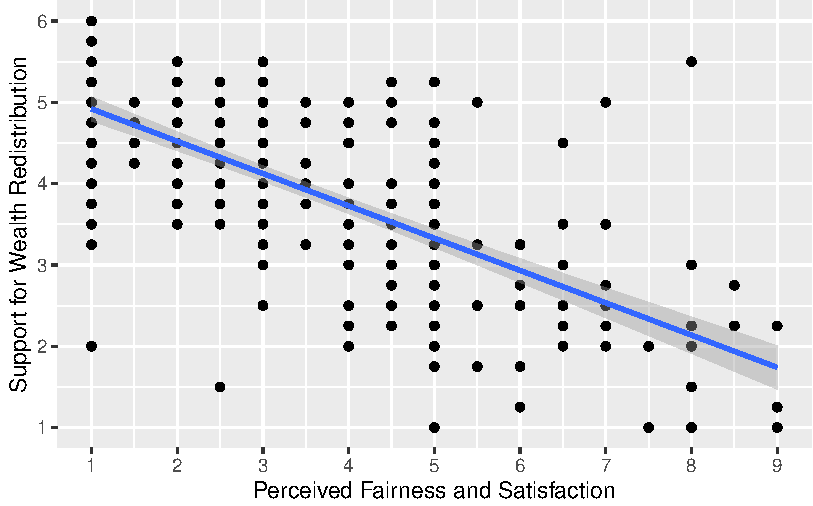
\includegraphics[width=1\textwidth,height=\textheight]{08-lm-continuous_files/figure-pdf/unnamed-chunk-5-1.pdf}
\end{center}

Looking at the graph, we can describe the relationship as

\begin{itemize}
\tightlist
\item
  \begin{enumerate}
  \def\labelenumi{(\Alph{enumi})}
  \tightlist
  \item
    positive\\
  \end{enumerate}
\item
  \begin{enumerate}
  \def\labelenumi{(\Alph{enumi})}
  \setcounter{enumi}{1}
  \tightlist
  \item
    little to no correlation\\
  \end{enumerate}
\item
  \begin{enumerate}
  \def\labelenumi{(\Alph{enumi})}
  \setcounter{enumi}{2}
  \tightlist
  \item
    negative
  \end{enumerate}
\end{itemize}

.

\end{tcolorbox}

\begin{tcolorbox}[enhanced jigsaw, breakable, colframe=quarto-callout-caution-color-frame, arc=.35mm, opacitybacktitle=0.6, titlerule=0mm, colbacktitle=quarto-callout-caution-color!10!white, colback=white, toprule=.15mm, bottomtitle=1mm, toptitle=1mm, title=\textcolor{quarto-callout-caution-color}{\faFire}\hspace{0.5em}{Show me the solution}, bottomrule=.15mm, rightrule=.15mm, leftrule=.75mm, coltitle=black, left=2mm, opacityback=0]

The scatterplot shows a negative correlation between the two variables.
You need to be careful interpreting fairness and satisfaction due to the
sneaky reverse-coding. Higher values mean \emph{greater} fairness and
satisfaction.

As support for wealth redistribution increases up the y-axis to be more
positive, perceived fairness and satisfaction tends to decrease on the
x-axis. In other words, for people who perceive things to be fair and
they are more satisfied, they are less supportive of reforms to wealth
redistribution.

You should have the following in a code chunk:

\begin{Shaded}
\begin{Highlighting}[]
\NormalTok{dawtry\_clean }\SpecialCharTok{\%\textgreater{}\%} 
  \FunctionTok{ggplot}\NormalTok{(}\FunctionTok{aes}\NormalTok{(}\AttributeTok{x =}\NormalTok{ fairness\_satisfaction, }\AttributeTok{y =}\NormalTok{ redistribution)) }\SpecialCharTok{+} 
  \FunctionTok{geom\_point}\NormalTok{() }\SpecialCharTok{+} 
  \FunctionTok{geom\_smooth}\NormalTok{(}\AttributeTok{method =} \StringTok{"lm"}\NormalTok{) }\SpecialCharTok{+} 
  \FunctionTok{scale\_x\_continuous}\NormalTok{(}\AttributeTok{name =} \StringTok{"Perceived Fairness and Satisfaction"}\NormalTok{, }
                     \AttributeTok{breaks =} \FunctionTok{c}\NormalTok{(}\DecValTok{1}\SpecialCharTok{:}\DecValTok{9}\NormalTok{)) }\SpecialCharTok{+} 
  \FunctionTok{scale\_y\_continuous}\NormalTok{(}\AttributeTok{name =} \StringTok{"Support for Wealth Redistribution"}\NormalTok{, }
                     \AttributeTok{breaks =} \FunctionTok{c}\NormalTok{(}\DecValTok{1}\SpecialCharTok{:}\DecValTok{6}\NormalTok{))}
\end{Highlighting}
\end{Shaded}

\end{tcolorbox}

\subsection{Activity 4 - Calculate the correlation
coefficient}\label{activity-4---calculate-the-correlation-coefficient}

Visualising the relationship between two variables is great for our
understanding, but it does not tell us anything about the inferential
statistics for what we can learn from our sample in hypothesis testing
and measures of effect size.

A correlation is a specific application of the general linear model. We
want to capture the covariation between two variables. If you are
interested, see the Handy Workbook
(\href{https://psyteachr.github.io/handyworkbook/pearson-correlation.html}{McAleer,
2023}) for the calculations behind different types of correlation and
how it represents the covariance of two variables compared to their
total variability. They are not the only methods, but the two most
common versions of a correlation are:

\begin{itemize}
\item
  Pearson's product-moment correlation (often shortened to the Pearson
  correlation) and symbolised by \textbf{r}.
\item
  Spearman's rank correlation coefficient (often shortened to the
  Spearman correlation) and symbolised by \(r_s\) or sometimes the Greek
  letter \textbf{rho} \(\rho\).
\end{itemize}

There is a function built into R (\texttt{cor.test()}) to calculate the
correlation between two variables, but we tend to use the
\texttt{correlation()} function from the correlation package as it has
more consistent reporting features. The \texttt{correlation()} function
requires:

\begin{itemize}
\item
  The name of the data set you are using.
\item
  The name of the first variable you want to select for the correlation.
\item
  The name of the second variable you want to select for the
  correlation.
\item
  The type of correlation you want to run: e.g.~\texttt{pearson},
  \texttt{spearman}.
\end{itemize}

For our \texttt{dawtry\_clean} data, we would run the following code for
a two-tailed Pearson correlation:

\begin{Shaded}
\begin{Highlighting}[]
\FunctionTok{correlation}\NormalTok{(}\AttributeTok{data =}\NormalTok{ dawtry\_clean, }
            \AttributeTok{select =} \StringTok{"fairness\_satisfaction"}\NormalTok{, }
            \AttributeTok{select2 =} \StringTok{"redistribution"}\NormalTok{,  }
            \AttributeTok{method =} \StringTok{"pearson"}\NormalTok{, }
            \AttributeTok{alternative =} \StringTok{"two.sided"}\NormalTok{)}
\end{Highlighting}
\end{Shaded}

\begin{verbatim}
Parameter1            |     Parameter2 |     r |         95% CI | t(303) |      p
---------------------------------------------------------------------------------
fairness_satisfaction | redistribution | -0.70 | [-0.75, -0.64] | -17.08 | < .001

Observations: 305
\end{verbatim}

Your output will look a little different due to how our book renders
tables, but you should get the same information. For the three key
concepts of inferential statistics, we get

\begin{itemize}
\item
  \textbf{Hypothesis testing}: \emph{p} \textless{} .001, suggesting we
  can reject the null hypothesis assuming \(\alpha\) = .05.
\item
  \textbf{Effect size}: \emph{r} = -.70, suggesting a strong negative
  correlation.
\item
  \textbf{Confidence interval}: {[}-0.75, -0.64{]}, showing the
  precision around the effect size estimate.
\end{itemize}

To summarise: a Pearson correlation showed there was a strong, negative,
statistically significant relationship between attitudes on wealth
redistribution and perceived fairness and satisfaction, \emph{r} (303) =
-0.70, \emph{p} \textless{} .001, 95\% CI = {[}-0.75, -0.64{]}.

If we had reason to use a Spearman correlation instead, all we need to
do is change the \texttt{method} argument.

\begin{Shaded}
\begin{Highlighting}[]
\FunctionTok{correlation}\NormalTok{(}\AttributeTok{data =}\NormalTok{ dawtry\_clean, }
            \AttributeTok{select =} \StringTok{"fairness\_satisfaction"}\NormalTok{, }
            \AttributeTok{select2 =} \StringTok{"redistribution"}\NormalTok{,  }
            \AttributeTok{method =} \StringTok{"spearman"}\NormalTok{, }
            \AttributeTok{alternative =} \StringTok{"two.sided"}\NormalTok{)}
\end{Highlighting}
\end{Shaded}

\begin{verbatim}
Parameter1            |     Parameter2 |   rho |         95% CI |        S |      p
-----------------------------------------------------------------------------------
fairness_satisfaction | redistribution | -0.68 | [-0.74, -0.61] | 7.95e+06 | < .001

Observations: 305
\end{verbatim}

Similarly, we could report the results as: a Spearman correlation showed
there was a strong, negative, statistically significant relationship
between attitudes on wealth redistribution and perceived fairness and
satisfaction, \(r_s\) (303) = -0.68, \emph{p} \textless{} .001, 95\% CI
= {[}-0.74, -0.61{]}.

\begin{tcolorbox}[enhanced jigsaw, breakable, colframe=quarto-callout-note-color-frame, arc=.35mm, opacitybacktitle=0.6, titlerule=0mm, colbacktitle=quarto-callout-note-color!10!white, colback=white, toprule=.15mm, bottomtitle=1mm, toptitle=1mm, title=\textcolor{quarto-callout-note-color}{\faInfo}\hspace{0.5em}{One-tailed tests}, bottomrule=.15mm, rightrule=.15mm, leftrule=.75mm, coltitle=black, left=2mm, opacityback=0]

By default, these functions will apply a two-tailed test to look for any
correlation value more extreme than zero - the null hypothesis - which
could be positive or negative. If you wanted to run a one-tailed
correlation and look for an effect in one specific direction, you would
use the argument \texttt{alternative\ =\ "greater"} for positive
correlations and \texttt{alternative\ =\ "less"} for negative
correlations.

\end{tcolorbox}

\begin{tcolorbox}[enhanced jigsaw, breakable, colframe=quarto-callout-tip-color-frame, arc=.35mm, opacitybacktitle=0.6, titlerule=0mm, colbacktitle=quarto-callout-tip-color!10!white, colback=white, toprule=.15mm, bottomtitle=1mm, toptitle=1mm, title=\textcolor{quarto-callout-tip-color}{\faLightbulb}\hspace{0.5em}{Try this}, bottomrule=.15mm, rightrule=.15mm, leftrule=.75mm, coltitle=black, left=2mm, opacityback=0]

Great work following along so far, but now it is time to test your
understanding on a new set of variables. Use the variables \texttt{age}
and \texttt{redistribution} from \texttt{dawtry\_clean}. We can ask the
question: ``What is the relationship between age and attitudes on wealth
redistribution?''

\begin{enumerate}
\def\labelenumi{\arabic{enumi}.}
\item
  Create a scatterplot to visualise the relationship between
  \texttt{age} and \texttt{redistribution} from \texttt{dawtry\_clean}.
\item
  Apply the Pearson correlation to get your inferential statistics and
  answer the following questions:

  \begin{itemize}
  \tightlist
  \item
    \textbf{Hypothesis testing}: Assuming \(\alpha\) = .05, the
    relationship between age and wealth redistribution is
  \end{itemize}
\end{enumerate}

\begin{itemize}
\tightlist
\item
  \begin{enumerate}
  \def\labelenumi{(\Alph{enumi})}
  \tightlist
  \item
    statistically significant\\
  \end{enumerate}
\item
  \begin{enumerate}
  \def\labelenumi{(\Alph{enumi})}
  \setcounter{enumi}{1}
  \tightlist
  \item
    not statistically significant
  \end{enumerate}
\end{itemize}

.

\begin{verbatim}
- **Effect size**: Rounded to 2 decimals, the value for Pearson's correlation coefficient is 
\end{verbatim}

\begin{itemize}
\tightlist
\item
  \begin{enumerate}
  \def\labelenumi{(\Alph{enumi})}
  \tightlist
  \item
    -0.14\\
  \end{enumerate}
\item
  \begin{enumerate}
  \def\labelenumi{(\Alph{enumi})}
  \setcounter{enumi}{1}
  \tightlist
  \item
    -0.03\\
  \end{enumerate}
\item
  \begin{enumerate}
  \def\labelenumi{(\Alph{enumi})}
  \setcounter{enumi}{2}
  \tightlist
  \item
    0.08\\
  \end{enumerate}
\item
  \begin{enumerate}
  \def\labelenumi{(\Alph{enumi})}
  \setcounter{enumi}{3}
  \tightlist
  \item
    -0.49
  \end{enumerate}
\end{itemize}

.

\begin{verbatim}
- **Confidence interval**: Rounded to 2 decimals, the lower bound is 
\end{verbatim}

\begin{itemize}
\tightlist
\item
  \begin{enumerate}
  \def\labelenumi{(\Alph{enumi})}
  \tightlist
  \item
    -0.14\\
  \end{enumerate}
\item
  \begin{enumerate}
  \def\labelenumi{(\Alph{enumi})}
  \setcounter{enumi}{1}
  \tightlist
  \item
    -0.03\\
  \end{enumerate}
\item
  \begin{enumerate}
  \def\labelenumi{(\Alph{enumi})}
  \setcounter{enumi}{2}
  \tightlist
  \item
    0.08\\
  \end{enumerate}
\item
  \begin{enumerate}
  \def\labelenumi{(\Alph{enumi})}
  \setcounter{enumi}{3}
  \tightlist
  \item
    -0.49
  \end{enumerate}
\end{itemize}

and the upper bound is

\begin{itemize}
\tightlist
\item
  \begin{enumerate}
  \def\labelenumi{(\Alph{enumi})}
  \tightlist
  \item
    -0.14\\
  \end{enumerate}
\item
  \begin{enumerate}
  \def\labelenumi{(\Alph{enumi})}
  \setcounter{enumi}{1}
  \tightlist
  \item
    -0.03\\
  \end{enumerate}
\item
  \begin{enumerate}
  \def\labelenumi{(\Alph{enumi})}
  \setcounter{enumi}{2}
  \tightlist
  \item
    0.08\\
  \end{enumerate}
\item
  \begin{enumerate}
  \def\labelenumi{(\Alph{enumi})}
  \setcounter{enumi}{3}
  \tightlist
  \item
    -0.49
  \end{enumerate}
\end{itemize}

.

\end{tcolorbox}

\begin{tcolorbox}[enhanced jigsaw, breakable, colframe=quarto-callout-caution-color-frame, arc=.35mm, opacitybacktitle=0.6, titlerule=0mm, colbacktitle=quarto-callout-caution-color!10!white, colback=white, toprule=.15mm, bottomtitle=1mm, toptitle=1mm, title=\textcolor{quarto-callout-caution-color}{\faFire}\hspace{0.5em}{Show me the solution}, bottomrule=.15mm, rightrule=.15mm, leftrule=.75mm, coltitle=black, left=2mm, opacityback=0]

The scatterplot shows very little correlation between the two variables.
The regression line is almost flat and there does not appear to be a
clear pattern to the data points.

\begin{Shaded}
\begin{Highlighting}[]
\NormalTok{dawtry\_clean }\SpecialCharTok{\%\textgreater{}\%} 
  \FunctionTok{ggplot}\NormalTok{(}\FunctionTok{aes}\NormalTok{(}\AttributeTok{x =}\NormalTok{ age, }\AttributeTok{y =}\NormalTok{ redistribution)) }\SpecialCharTok{+} 
  \FunctionTok{geom\_point}\NormalTok{() }\SpecialCharTok{+} 
  \FunctionTok{geom\_smooth}\NormalTok{(}\AttributeTok{method =} \StringTok{"lm"}\NormalTok{) }\SpecialCharTok{+} 
  \FunctionTok{scale\_y\_continuous}\NormalTok{(}\AttributeTok{name =} \StringTok{"Attitudes on Wealth Distribution"}\NormalTok{, }
                     \AttributeTok{breaks =} \FunctionTok{c}\NormalTok{(}\DecValTok{1}\SpecialCharTok{:}\DecValTok{6}\NormalTok{))}
\end{Highlighting}
\end{Shaded}

\begin{center}
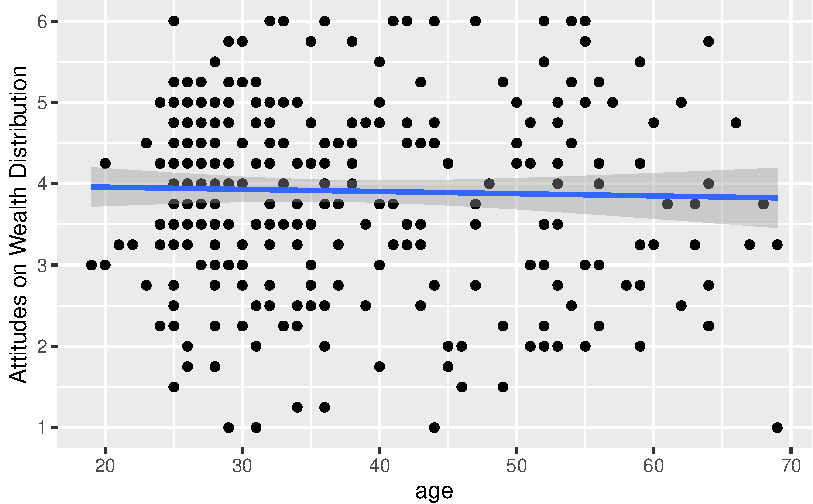
\includegraphics[width=1\textwidth,height=\textheight]{08-lm-continuous_files/figure-pdf/unnamed-chunk-11-1.pdf}
\end{center}

For our inferential statistics, the relationship is not statistically
significant and the Pearson correlation coefficient is very weak,
\emph{r} (302) = -0.03, \emph{p} = .625, 95\% CI = {[}-0.14, 0.08{]}.
Note there is a missing value for age, so we have one fewer participant
/ degrees of freedom.

\begin{Shaded}
\begin{Highlighting}[]
\FunctionTok{correlation}\NormalTok{(}\AttributeTok{data =}\NormalTok{ dawtry\_clean, }
            \AttributeTok{select =} \StringTok{"age"}\NormalTok{, }
            \AttributeTok{select2 =} \StringTok{"redistribution"}\NormalTok{,  }
            \AttributeTok{method =} \StringTok{"pearson"}\NormalTok{, }
            \AttributeTok{alternative =} \StringTok{"two.sided"}\NormalTok{)}
\end{Highlighting}
\end{Shaded}

\begin{verbatim}
# Correlation Matrix (pearson-method)

Parameter1 |     Parameter2 |     r |        95% CI | t(302) |     p
--------------------------------------------------------------------
age        | redistribution | -0.03 | [-0.14, 0.08] |  -0.49 | 0.625

p-value adjustment method: Holm (1979)
Observations: 304
\end{verbatim}

\end{tcolorbox}

\subsection{Reporting your correlation
reproducibly}\label{reporting-your-correlation-reproducibly}

When you write reports, you can take the numbers from your output and
type them out but it is easy to make typos or forget to update your
numbers. By writing reproducible reports in R, you can avoid this by
adding a little code to format the numbers into APA format.

For correlations, the first step is saving your \texttt{correlation()}
function as an object.

\begin{Shaded}
\begin{Highlighting}[]
\NormalTok{fairness\_redist\_object }\OtherTok{\textless{}{-}} \FunctionTok{correlation}\NormalTok{(}\AttributeTok{data =}\NormalTok{ dawtry\_clean, }
                                      \AttributeTok{select =} \StringTok{"fairness\_satisfaction"}\NormalTok{, }
                                      \AttributeTok{select2 =} \StringTok{"redistribution"}\NormalTok{,  }
                                      \AttributeTok{method =} \StringTok{"pearson"}\NormalTok{, }
                                      \AttributeTok{alternative =} \StringTok{"two.sided"}\NormalTok{)}
\end{Highlighting}
\end{Shaded}

If you look in the Environment, the correlation package helpfully saves
the output as a data frame which makes it easy to work with. For the
following code, this is a function we have created, so we do not expect
you to understand everything at this point. You just need to copy and
paste it into your .Rmd file before you want to reference the
correlation. Click show the correlation formatting function as we
initially hide it to avoid taking up lots of space.

\begin{Shaded}
\begin{Highlighting}[]
\NormalTok{report\_correlation }\OtherTok{\textless{}{-}} \ControlFlowTok{function}\NormalTok{(correlation\_object)\{}
  \CommentTok{\# This function will only work for correlation package objects}
  \CommentTok{\# Step 1 = save all the numbers with formatting }
\NormalTok{  r\_type }\OtherTok{\textless{}{-}} \FunctionTok{ifelse}\NormalTok{(correlation\_object}\SpecialCharTok{$}\NormalTok{Method }\SpecialCharTok{==} \StringTok{"Pearson correlation"}\NormalTok{, }
                   \StringTok{"*r* "}\NormalTok{, }\CommentTok{\# if true, report as Pearson correlation}
                   \StringTok{"*r\_s* "}\NormalTok{) }\CommentTok{\# if false, report as Spearman correlation}
  \CommentTok{\# save degrees of freedom}
\NormalTok{  df }\OtherTok{\textless{}{-}}\NormalTok{ correlation\_object}\SpecialCharTok{$}\NormalTok{df\_error}
  \CommentTok{\# save r rounded to 3 decimals with any trailing zeros}
\NormalTok{  r }\OtherTok{\textless{}{-}} \FunctionTok{sprintf}\NormalTok{(}\StringTok{"\%.3f"}\NormalTok{, }\FunctionTok{round}\NormalTok{(correlation\_object}\SpecialCharTok{$}\NormalTok{r, }\DecValTok{3}\NormalTok{))}
  \CommentTok{\# save p value with formatting if less than .001}
\NormalTok{  pval }\OtherTok{\textless{}{-}}\NormalTok{ correlation\_object}\SpecialCharTok{$}\NormalTok{p}
  \ControlFlowTok{if}\NormalTok{ (pval }\SpecialCharTok{\textgreater{}=} \FloatTok{0.001}\NormalTok{)\{}
\NormalTok{    pval }\OtherTok{\textless{}{-}} \FunctionTok{str\_sub}\NormalTok{(}\FunctionTok{as.character}\NormalTok{(pval), }\DecValTok{2}\NormalTok{, }\DecValTok{5}\NormalTok{)}
\NormalTok{    pval }\OtherTok{\textless{}{-}}  \FunctionTok{paste0}\NormalTok{(}\StringTok{", *p* = "}\NormalTok{, pval)}
  \CommentTok{\# If p \textless{} .001, manually format as p \textless{} .001}
\NormalTok{  \} }\ControlFlowTok{else} \ControlFlowTok{if}\NormalTok{ (pval }\SpecialCharTok{\textless{}} \FloatTok{0.001}\NormalTok{)\{}
\NormalTok{    pval }\OtherTok{\textless{}{-}} \StringTok{", *p* \textless{} .001"}
\NormalTok{  \}}
  \CommentTok{\# save lower 95\% CI}
\NormalTok{  lower\_CI }\OtherTok{\textless{}{-}} \FunctionTok{round}\NormalTok{(correlation\_object}\SpecialCharTok{$}\NormalTok{CI\_low, }\DecValTok{3}\NormalTok{)}
  \CommentTok{\# save lower 95\% CI}
\NormalTok{  upper\_CI }\OtherTok{\textless{}{-}} \FunctionTok{round}\NormalTok{(correlation\_object}\SpecialCharTok{$}\NormalTok{CI\_high, }\DecValTok{3}\NormalTok{)}
  \CommentTok{\# Switch CIs depending on sign }
\NormalTok{  r\_CI }\OtherTok{\textless{}{-}} \FunctionTok{ifelse}\NormalTok{(r }\SpecialCharTok{\textgreater{}} \DecValTok{0}\NormalTok{,}
                 \FunctionTok{paste0}\NormalTok{(lower\_CI, }\StringTok{", "}\NormalTok{, upper\_CI),}
                 \FunctionTok{paste0}\NormalTok{(upper\_CI, }\StringTok{", "}\NormalTok{, lower\_CI))}
  
  \CommentTok{\# Step 2 = add them together in APA format}
\NormalTok{  output }\OtherTok{\textless{}{-}} \FunctionTok{paste0}\NormalTok{(r\_type, }
                   \StringTok{"("}\NormalTok{, df,}\StringTok{") = "}\NormalTok{,}
\NormalTok{                   r,}
\NormalTok{                   pval,}
                   \StringTok{", 95\% CI = ["}\NormalTok{, r\_CI, }\StringTok{"]"}\NormalTok{)}
  
  \FunctionTok{return}\NormalTok{(output)}
\NormalTok{\}}
\end{Highlighting}
\end{Shaded}

Once you have saved the object and added the formatting function, you
can use the function to format your correlation:

\begin{Shaded}
\begin{Highlighting}[]
\FunctionTok{report\_correlation}\NormalTok{(fairness\_redist\_object)}
\end{Highlighting}
\end{Shaded}

\begin{verbatim}
[1] "*r* (303) = -0.700, *p* < .001, 95% CI = [-0.638, -0.753]"
\end{verbatim}

You can add that as inline code to insert into your report to make your
inferential statistics reproducible. Just note it's difficult to apply
all the APA format details, so you might need to remove leading zeros,
add italics to the math symbols etc.

\section{Linear regression with one continuous
predictor}\label{linear-regression-with-one-continuous-predictor}

Now you know how to calculate a correlation in R, we can turn to simple
linear regression as a more flexible tool for modelling the relationship
between variables.

In Research Methods 1, we focus on just two variables, before scaling up
to more complicated models in Research Methods 2. In this chapter, we
focus the relationship between a continuous outcome and one continuous
predictor, before extending the framework to one categorical predictor
in Chapter 9. There is also a chapter in the Handy Workbook
(\href{https://psyteachr.github.io/handyworkbook/simple-linear-regression.html}{McAleer,
2023}) dedicated to manually calculating simple linear regression.

\subsection{Activity 5- Calculating descriptive
statistics}\label{activity-5--calculating-descriptive-statistics}

For all the information we want to include in a report, calculating
descriptive statistics is helpful for the reader to show the context
behind the results you present. Here, we can report the mean and
standard deviation of our two variables.

\begin{Shaded}
\begin{Highlighting}[]
\NormalTok{dawtry\_clean }\SpecialCharTok{\%\textgreater{}\%} 
  \CommentTok{\# pivot longer to avoid repeating yourself}
  \FunctionTok{pivot\_longer}\NormalTok{(}\AttributeTok{cols =}\NormalTok{ fairness\_satisfaction}\SpecialCharTok{:}\NormalTok{redistribution,}
               \AttributeTok{names\_to =} \StringTok{"Variable"}\NormalTok{, }
               \AttributeTok{values\_to =} \StringTok{"Value"}\NormalTok{) }\SpecialCharTok{\%\textgreater{}\%} 
  \CommentTok{\# group by Variable to get one value per variable}
  \FunctionTok{group\_by}\NormalTok{(Variable) }\SpecialCharTok{\%\textgreater{}\%} 
  \CommentTok{\# mean and SD, rounded to 2 decimals}
  \FunctionTok{summarise}\NormalTok{(}\AttributeTok{mean\_variable =} \FunctionTok{round}\NormalTok{(}\FunctionTok{mean}\NormalTok{(Value), }\DecValTok{2}\NormalTok{),}
            \AttributeTok{sd\_variable =} \FunctionTok{round}\NormalTok{(}\FunctionTok{sd}\NormalTok{(Value), }\DecValTok{2}\NormalTok{))}
\end{Highlighting}
\end{Shaded}

\begin{verbatim}
# A tibble: 2 x 3
  Variable              mean_variable sd_variable
  <chr>                         <dbl>       <dbl>
1 fairness_satisfaction          3.54        2.02
2 redistribution                 3.91        1.15
\end{verbatim}

\begin{tcolorbox}[enhanced jigsaw, breakable, colframe=quarto-callout-note-color-frame, arc=.35mm, opacitybacktitle=0.6, titlerule=0mm, colbacktitle=quarto-callout-note-color!10!white, colback=white, toprule=.15mm, bottomtitle=1mm, toptitle=1mm, title=\textcolor{quarto-callout-note-color}{\faInfo}\hspace{0.5em}{Note}, bottomrule=.15mm, rightrule=.15mm, leftrule=.75mm, coltitle=black, left=2mm, opacityback=0]

If you want some reinforcement of how these skills apply to published
research, look at Table 1 in Dawtry et al. (2015). The means and
standard deviations here (and the correlation in Activity 4) exactly
reproduce the values they report.

\end{tcolorbox}

If other types of descriptive statistic would be more suitable to your
data, then you can just replace the functions you use within
\texttt{summarise()}.

\subsection{\texorpdfstring{Activity 6 - Using the \texttt{lm()}
function}{Activity 6 - Using the lm() function}}\label{activity-6---using-the-lm-function}

For our research question of ``is there a relationship between support
for wealth redistribution and fairness and satisfaction'', we can
address it with simple linear regression.

Instead of a standardised correlation coefficient, we can frame it as
whether knowing fairness and satisfaction can predict values of support
for wealth redistribution. The design is still correlational, so it does
not tell us anything about a causal relationship in isolation. We use
the word predict in the statistical sense, where we can ask whether
knowing values of one variable help us predict values of another
variable with a degree of error.

The first step is to create an object (\texttt{lm\_redistribution}) for
the linear model.

\begin{Shaded}
\begin{Highlighting}[]
\NormalTok{lm\_redistribution }\OtherTok{\textless{}{-}} \FunctionTok{lm}\NormalTok{(redistribution }\SpecialCharTok{\textasciitilde{}}\NormalTok{ fairness\_satisfaction,}
                        \AttributeTok{data =}\NormalTok{ dawtry\_clean)}
\end{Highlighting}
\end{Shaded}

The function \texttt{lm()} is built into R and is incredibly flexible
for creating linear regression models.

\begin{itemize}
\item
  The first argument is to specify a formula which defines our model.
  The first component (\texttt{redistribution}) is our outcome variable
  for what we are interested in modelling.
\item
  The tilde (\texttt{\textasciitilde{}}) separates the equation, where
  everything on the right is your predictor variable(s). In simple
  linear regression, we just have one predictor, which is
  \texttt{fairness\_satisfaction} in our model here. This is saying we
  want to predict \texttt{redistribution} as our outcome from
  \texttt{fairness\_satisfaction} as our predictor.
\item
  We then specify the data frame we want to use.
\end{itemize}

\begin{tcolorbox}[enhanced jigsaw, breakable, colframe=quarto-callout-note-color-frame, arc=.35mm, opacitybacktitle=0.6, titlerule=0mm, colbacktitle=quarto-callout-note-color!10!white, colback=white, toprule=.15mm, bottomtitle=1mm, toptitle=1mm, title=\textcolor{quarto-callout-note-color}{\faInfo}\hspace{0.5em}{Note}, bottomrule=.15mm, rightrule=.15mm, leftrule=.75mm, coltitle=black, left=2mm, opacityback=0]

In some resources, you might see people enter the same model as
\texttt{redistribution\ \textasciitilde{}\ 1\ +\ fairness\_satisfaction}.
The \texttt{1\ +} component explicitly tells R to fit an intercept, plus
a slope from \texttt{fairness\_satisfaction}. R includes an intercept by
default, so you do not need to add it, but some people like to include
it for clarity.

\end{tcolorbox}

When you create this object, it stores a bunch of information, but does
not really tell us all the statistics we expect. If you simply print the
object in the console, it will tell you the intercept and
coefficient(s), but none of the model fitting nor hypothesis testing
values. If you look at the object in the R environment, you will see it
is a list containing several elements. It stores things like the model,
the residuals, and other information you can use.

\begin{Shaded}
\begin{Highlighting}[]
\NormalTok{lm\_redistribution}
\end{Highlighting}
\end{Shaded}

\begin{verbatim}

Call:
lm(formula = redistribution ~ fairness_satisfaction, data = dawtry_clean)

Coefficients:
          (Intercept)  fairness_satisfaction  
               5.3169                -0.3975  
\end{verbatim}

To get that extra information, we need to call the \texttt{summary()}
function around the linear model object to explore it's properties like
estimates and model fit.

\begin{Shaded}
\begin{Highlighting}[]
\FunctionTok{summary}\NormalTok{(lm\_redistribution)}
\end{Highlighting}
\end{Shaded}

\begin{verbatim}

Call:
lm(formula = redistribution ~ fairness_satisfaction, data = dawtry_clean)

Residuals:
    Min      1Q  Median      3Q     Max 
-2.9193 -0.5279  0.0233  0.4782  3.3634 

Coefficients:
                      Estimate Std. Error t value Pr(>|t|)    
(Intercept)            5.31686    0.09488   56.04   <2e-16 ***
fairness_satisfaction -0.39754    0.02328  -17.08   <2e-16 ***
---
Signif. codes:  0 '***' 0.001 '**' 0.01 '*' 0.05 '.' 0.1 ' ' 1

Residual standard error: 0.8218 on 303 degrees of freedom
Multiple R-squared:  0.4905,    Adjusted R-squared:  0.4888 
F-statistic: 291.7 on 1 and 303 DF,  p-value: < 2.2e-16
\end{verbatim}

To walk through the output, \texttt{Call:} summarises the model you
specified. \texttt{Residuals:} provides a summary of the model residuals
which we will come back to later. \texttt{Coefficients:} provides our
model output, this time with inferential statistics. The two key lines
are:

\begin{enumerate}
\def\labelenumi{\arabic{enumi}.}
\tightlist
\item
  \texttt{(Intercept)} - This is the value of the outcome when our
  predictor is set to 0. For a fairness and satisfaction value of 0, we
  would expect a value of 5.32 for redistribution. You get a
  \emph{p}-value for this, but in isolation it is not too useful. It
  just compares the intercept estimate to 0 which typically you are not
  interested in.
\end{enumerate}

\begin{itemize}
\tightlist
\item
  \texttt{fairness\_satisfaction} - This is the regression slope or
  coefficient. This is the change in the outcome for every 1 unit change
  in the predictor. So, for every 1 unit increase in fairness and
  satisfaction, we expect support for wealth redistribution to decrease
  (as we have a negative value) by 0.40 units. This is consistent with
  the correlation as we have a negative relationship between the two
  variables. Looking at the \emph{p}-value, this is statistically
  significant (\emph{p} \textless{} .001), suggesting we can reject the
  null hypothesis and conclude there is an effect here.
\end{itemize}

\begin{tcolorbox}[enhanced jigsaw, breakable, colframe=quarto-callout-note-color-frame, arc=.35mm, opacitybacktitle=0.6, titlerule=0mm, colbacktitle=quarto-callout-note-color!10!white, colback=white, toprule=.15mm, bottomtitle=1mm, toptitle=1mm, title=\textcolor{quarto-callout-note-color}{\faInfo}\hspace{0.5em}{Does it matter if the slope is positive or negative?}, bottomrule=.15mm, rightrule=.15mm, leftrule=.75mm, coltitle=black, left=2mm, opacityback=0]

When you have a continuous predictor, the sign is important to keep in
mind. A positive slope would mean an increase in the predictor is
associated with increased values of your outcome. A negative slope would
mean an increase in the predictor is associated with decreased values of
your outcome. This is crucial for interpreting the coefficient.

\end{tcolorbox}

At the bottom of the model output, you then get the fit statistics.
Multiple \(R^2\) tells you how much variance in your outcome your
predictor(s) explain. Adjusted \(R^2\) tends to be more conservative as
it adjusts for the number of predictors in the model (something we will
not cover until Chapter 14), but they will be very similar when you have
one predictor. Adjusted \(R^2\) is .49, suggesting fairness and
satisfaction explains 49\% of the variance in support for wealth
redistribution.

Finally, we have the model fit statistics to tell us whether the model
explains a significant amount of variance in the outcome. With one
predictor, the \emph{p}-value next to the coefficient and next to the
model fit will be identical, as one predictor is the whole model. The
F-statistic is 291.7, the model degrees of freedom is 1, the residual
degrees of freedom is 303, and the \emph{p}-value is \emph{p}
\textless{} .001.

\begin{tcolorbox}[enhanced jigsaw, breakable, colframe=quarto-callout-important-color-frame, arc=.35mm, opacitybacktitle=0.6, titlerule=0mm, colbacktitle=quarto-callout-important-color!10!white, colback=white, toprule=.15mm, bottomtitle=1mm, toptitle=1mm, title=\textcolor{quarto-callout-important-color}{\faExclamation}\hspace{0.5em}{What does 2e-16 mean?}, bottomrule=.15mm, rightrule=.15mm, leftrule=.75mm, coltitle=black, left=2mm, opacityback=0]

For the \emph{p}-value here, the output looks a little weird. R reports
very small or very large numbers using scientific notation to save
space. We normally report \emph{p}-values to three decimals, so we
report anything smaller as \emph{p} \textless{} .001 to say it is
smaller than this.

If you want to see the real number, you can use the following function
which shows just how small the \emph{p}-value is:

\begin{Shaded}
\begin{Highlighting}[]
\FunctionTok{format}\NormalTok{(}\FloatTok{2e{-}16}\NormalTok{, }\AttributeTok{scientific =} \ConstantTok{FALSE}\NormalTok{)}
\end{Highlighting}
\end{Shaded}

\begin{verbatim}
[1] "0.0000000000000002"
\end{verbatim}

\end{tcolorbox}

\begin{tcolorbox}[enhanced jigsaw, breakable, colframe=quarto-callout-note-color-frame, arc=.35mm, opacitybacktitle=0.6, titlerule=0mm, colbacktitle=quarto-callout-note-color!10!white, colback=white, toprule=.15mm, bottomtitle=1mm, toptitle=1mm, title=\textcolor{quarto-callout-note-color}{\faInfo}\hspace{0.5em}{How are correlation and regression the same?}, bottomrule=.15mm, rightrule=.15mm, leftrule=.75mm, coltitle=black, left=2mm, opacityback=0]

If you are interested in the relationship between the two concepts, we
said correlation was a specific application of the general linear model.
It describes the - standardised - covariation between two variables
compared to their total variability. For values of -1 and 1, knowing the
value of one variable perfectly correlates to the value of your other
variable. As you approach 0, the relationship between the variables is
less perfect, meaning there is more variability left over compared to
the covariance.

In regression, we frame it as how much variance you explain compared to
the total amount of variance. The more variance your predictor explains,
the less unexplained variance there is left over. We no longer calculate
\emph{r}, we calculate \(R^2\) as the proportion of variance in your
outcome explained by your model. A value of 0 would be you explain no
variance and a value of 1 means you explain all the variance.

You can see the connection between the two by comparing the value of
Pearson's \emph{r} from Activity 4 (-.70) to the value of \(R^2\) =
.4905. If you take the square root to get \emph{r}
(\texttt{sqrt(.4905)}), you get .70, which is exactly the same absolute
value since \(R^2\) can only be positive.

So, when you have a single continuous predictor, it is the exact same
process as correlation, just expressed slightly different.

\end{tcolorbox}

\subsection{Activity 7 - Calculating confidence
intervals}\label{activity-7---calculating-confidence-intervals}

In the standard \texttt{lm()} and \texttt{summary()} output, we get most
of the key values we need for our inferential statistics, but the one
thing missing is confidence intervals around our estimates. Fortunately,
R has a built-in function called \texttt{confint()} for calculating
confidence intervals using your linear model object.

\begin{Shaded}
\begin{Highlighting}[]
\FunctionTok{confint}\NormalTok{(lm\_redistribution)}
\end{Highlighting}
\end{Shaded}

\begin{verbatim}
                           2.5 %     97.5 %
(Intercept)            5.1301581  5.5035664
fairness_satisfaction -0.4433442 -0.3517332
\end{verbatim}

Normally, you focus on the confidence interval around your slope
estimate as the intercept is not usually super useful for interpreting
your findings when you have a continuous predictor. Now, we can
summarise the three key concepts of inferential statistics as:

\begin{itemize}
\item
  \textbf{Hypothesis testing}: \emph{p} \textless{} .001, suggesting we
  can reject the null hypothesis assuming \(\alpha\) = .05. Fairness and
  satisfaction is a significant predictor of support for wealth
  redistribution.
\item
  \textbf{Effect size}: \(b_1\) = -0.40, suggesting fairness and
  satisfaction is a negative predictor.
\item
  \textbf{Confidence interval}: {[}-0.44, -0.35{]}, showing the
  precision around the slope estimate.
\end{itemize}

\begin{tcolorbox}[enhanced jigsaw, breakable, colframe=quarto-callout-tip-color-frame, arc=.35mm, opacitybacktitle=0.6, titlerule=0mm, colbacktitle=quarto-callout-tip-color!10!white, colback=white, toprule=.15mm, bottomtitle=1mm, toptitle=1mm, title=\textcolor{quarto-callout-tip-color}{\faLightbulb}\hspace{0.5em}{Try this}, bottomrule=.15mm, rightrule=.15mm, leftrule=.75mm, coltitle=black, left=2mm, opacityback=0]

Great work following along so far, but now it is time to test your
understanding on a new set of variables. This time, use
\texttt{redistribution} as your outcome, \texttt{age} as your predictor,
and use \texttt{dawtry\_clean} as your data. We can ask the same
question as before: ``What is the relationship between age and attitudes
on wealth redistribution?''.

Apply simple linear regression to get your inferential statistics and
answer the following questions:

\begin{itemize}
\item
  \textbf{Hypothesis testing}: Assuming \(\alpha\) = .05, age is a
\item
  \begin{enumerate}
  \def\labelenumi{(\Alph{enumi})}
  \tightlist
  \item
    statistically significant\\
  \end{enumerate}
\item
  \begin{enumerate}
  \def\labelenumi{(\Alph{enumi})}
  \setcounter{enumi}{1}
  \tightlist
  \item
    non-significant
  \end{enumerate}
\end{itemize}

predictor of support for wealth redistribution.

\begin{itemize}
\item
  \textbf{Effect size}: Rounded to 2 decimals, the age coefficient is
\item
  \begin{enumerate}
  \def\labelenumi{(\Alph{enumi})}
  \tightlist
  \item
    4.01\\
  \end{enumerate}
\item
  \begin{enumerate}
  \def\labelenumi{(\Alph{enumi})}
  \setcounter{enumi}{1}
  \tightlist
  \item
    -0.003\\
  \end{enumerate}
\item
  \begin{enumerate}
  \def\labelenumi{(\Alph{enumi})}
  \setcounter{enumi}{2}
  \tightlist
  \item
    0.005\\
  \end{enumerate}
\item
  \begin{enumerate}
  \def\labelenumi{(\Alph{enumi})}
  \setcounter{enumi}{3}
  \tightlist
  \item
    0.22
  \end{enumerate}
\end{itemize}

.

\begin{itemize}
\item
  \textbf{Confidence interval}: Rounded to 2 decimals, the lower bound
  of the age coefficient is
\item
  \begin{enumerate}
  \def\labelenumi{(\Alph{enumi})}
  \tightlist
  \item
    3.59\\
  \end{enumerate}
\item
  \begin{enumerate}
  \def\labelenumi{(\Alph{enumi})}
  \setcounter{enumi}{1}
  \tightlist
  \item
    -0.01\\
  \end{enumerate}
\item
  \begin{enumerate}
  \def\labelenumi{(\Alph{enumi})}
  \setcounter{enumi}{2}
  \tightlist
  \item
    4.44\\
  \end{enumerate}
\item
  \begin{enumerate}
  \def\labelenumi{(\Alph{enumi})}
  \setcounter{enumi}{3}
  \tightlist
  \item
    0.01
  \end{enumerate}
\end{itemize}

and the upper bound is

\begin{itemize}
\tightlist
\item
  \begin{enumerate}
  \def\labelenumi{(\Alph{enumi})}
  \tightlist
  \item
    3.59\\
  \end{enumerate}
\item
  \begin{enumerate}
  \def\labelenumi{(\Alph{enumi})}
  \setcounter{enumi}{1}
  \tightlist
  \item
    -0.01\\
  \end{enumerate}
\item
  \begin{enumerate}
  \def\labelenumi{(\Alph{enumi})}
  \setcounter{enumi}{2}
  \tightlist
  \item
    4.44\\
  \end{enumerate}
\item
  \begin{enumerate}
  \def\labelenumi{(\Alph{enumi})}
  \setcounter{enumi}{3}
  \tightlist
  \item
    0.01
  \end{enumerate}
\end{itemize}

.

\end{tcolorbox}

\begin{tcolorbox}[enhanced jigsaw, breakable, colframe=quarto-callout-caution-color-frame, arc=.35mm, opacitybacktitle=0.6, titlerule=0mm, colbacktitle=quarto-callout-caution-color!10!white, colback=white, toprule=.15mm, bottomtitle=1mm, toptitle=1mm, title=\textcolor{quarto-callout-caution-color}{\faFire}\hspace{0.5em}{Show me the solution}, bottomrule=.15mm, rightrule=.15mm, leftrule=.75mm, coltitle=black, left=2mm, opacityback=0]

The conclusions are the same as when we calculated the correlation where
age is not a statistically significant predictor of support for wealth
redistribution. As a regression model, we get the same conclusions
expressed in a slightly different way. Age is negative, but the size of
the slope is very small (-0.003) and non-significant (\emph{p} = .625).
We explain pretty much no variance in support for wealth redistribution
(\(R^2\) = .0008), so age is not very informative as a predictor.

\begin{Shaded}
\begin{Highlighting}[]
\CommentTok{\# Create lm object for age as a predictor}
\NormalTok{lm\_age }\OtherTok{\textless{}{-}} \FunctionTok{lm}\NormalTok{(redistribution }\SpecialCharTok{\textasciitilde{}}\NormalTok{ age,}
             \AttributeTok{data =}\NormalTok{ dawtry\_clean)}

\CommentTok{\# summary of the model object}
\FunctionTok{summary}\NormalTok{(lm\_age)}

\CommentTok{\# confidence intervals around estimates}
\FunctionTok{confint}\NormalTok{(lm\_age)}
\end{Highlighting}
\end{Shaded}

\begin{verbatim}

Call:
lm(formula = redistribution ~ age, data = dawtry_clean)

Residuals:
     Min       1Q   Median       3Q      Max 
-2.93382 -0.69527  0.08099  0.84379  2.13621 

Coefficients:
             Estimate Std. Error t value Pr(>|t|)    
(Intercept)  4.011931   0.216042   18.57   <2e-16 ***
age         -0.002693   0.005499   -0.49    0.625    
---
Signif. codes:  0 '***' 0.001 '**' 0.01 '*' 0.05 '.' 0.1 ' ' 1

Residual standard error: 1.153 on 302 degrees of freedom
  (1 observation deleted due to missingness)
Multiple R-squared:  0.0007938, Adjusted R-squared:  -0.002515 
F-statistic: 0.2399 on 1 and 302 DF,  p-value: 0.6246

                  2.5 %     97.5 %
(Intercept)  3.58679351 4.43706821
age         -0.01351424 0.00812738
\end{verbatim}

\end{tcolorbox}

\subsection{Activity 8 - Centering and standardising
predictors}\label{activity-8---centering-and-standardising-predictors}

So far, we have covered specifying your outcome and predictor variables
as their raw values in the data. However, there are two variations that
are useful to understand: centering and standardising predictors. These
do not change the model fitting or \emph{p}-values, but change how you
interpret the intercept and/or slope.

\subsubsection{Centering predictors}\label{centering-predictors}

Centering predictors is where you change the values of your predictor,
but not their scale. Typically, this means substracting the mean of your
predictor from each observation. This changes how you interpret the
intercept of your regression model.

Remember the interpretation of the intercept is the predicted value of
your outcome when your predictor is set to 0. If 0 is not present in
your data or a value of 0 would be uninformative, the intercept can be
difficult to interpret. When you center your predictor, 0 becomes the
mean value of your predictor. So, the intercept is now the predicted
value of your outcome for the mean value of your predictor, but the
slope itself does not change. You can see the impact of this by plotting
the data side by side in Figure~\ref{fig-centering-predictors}.

\begin{Shaded}
\begin{Highlighting}[]
\NormalTok{dawtry\_clean }\OtherTok{\textless{}{-}}\NormalTok{ dawtry\_clean }\SpecialCharTok{\%\textgreater{}\%} 
  \CommentTok{\# subtract fairness values from mean of fairness}
  \FunctionTok{mutate}\NormalTok{(}\AttributeTok{fairness\_center =}\NormalTok{ fairness\_satisfaction }\SpecialCharTok{{-}} \FunctionTok{mean}\NormalTok{(fairness\_satisfaction))}
\end{Highlighting}
\end{Shaded}

\begin{figure}

\centering{

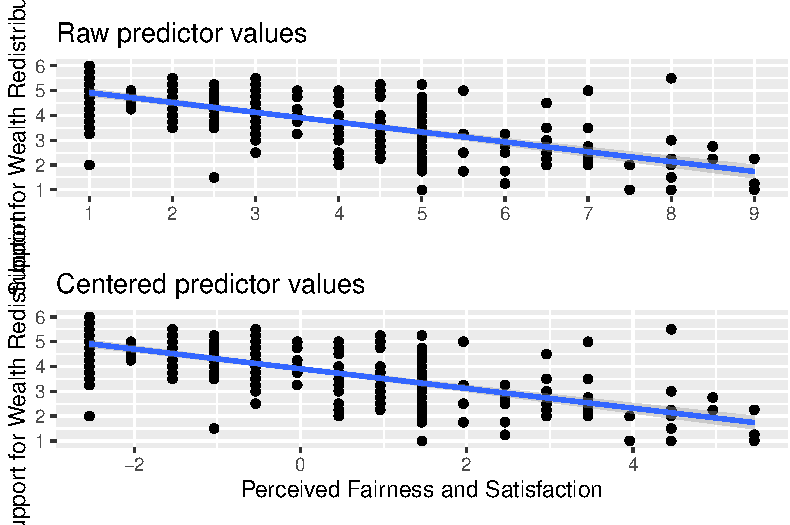
\includegraphics[width=1\textwidth,height=\textheight]{08-lm-continuous_files/figure-pdf/fig-centering-predictors-1.pdf}

}

\caption{\label{fig-centering-predictors}Top: The relationship between
wealth redistribution and perceived fairness and satisfaction using raw
values. Bottom: The relationship after centering perceived fairness and
satisfaction values.}

\end{figure}%

The relationship between the two variables is exactly the same, but the
values of fairness and satisfaction shifted so the mean is 0. If you
create a new linear model object, you can see the difference this makes
to the output.

\begin{Shaded}
\begin{Highlighting}[]
\NormalTok{lm\_center }\OtherTok{\textless{}{-}} \FunctionTok{lm}\NormalTok{(redistribution }\SpecialCharTok{\textasciitilde{}}\NormalTok{ fairness\_center, }
                \AttributeTok{data =}\NormalTok{ dawtry\_clean)}

\FunctionTok{summary}\NormalTok{(lm\_center)}
\end{Highlighting}
\end{Shaded}

\begin{verbatim}

Call:
lm(formula = redistribution ~ fairness_center, data = dawtry_clean)

Residuals:
    Min      1Q  Median      3Q     Max 
-2.9193 -0.5279  0.0233  0.4782  3.3634 

Coefficients:
                Estimate Std. Error t value Pr(>|t|)    
(Intercept)      3.90984    0.04706   83.09   <2e-16 ***
fairness_center -0.39754    0.02328  -17.08   <2e-16 ***
---
Signif. codes:  0 '***' 0.001 '**' 0.01 '*' 0.05 '.' 0.1 ' ' 1

Residual standard error: 0.8218 on 303 degrees of freedom
Multiple R-squared:  0.4905,    Adjusted R-squared:  0.4888 
F-statistic: 291.7 on 1 and 303 DF,  p-value: < 2.2e-16
\end{verbatim}

Every single one of the values remains the same apart from the
intercept. Now, we can interpret it as the predicted value of
redistribution when fairness and satisfaction is set to 0, i.e., the
mean value. So, for the mean value of fairness and satisfaction, we
would predict a value of 3.91 for redistribution.

\subsubsection{Standardising predictors}\label{standardising-predictors}

Standardising predictors is where you first convert your values to
z-scores. This means you interpret the values as standard deviations
rather than your original units. This is more useful in multiple
regression (Chapter 14) to compare the magnitude of predictors, but it
is useful to get used to now when you only have one predictor to focus
on.

The first step is to standardise \textbf{all} your variables, not just
the predictor this time. This involves subtracting the mean of your
variable from each value, and dividing by the standard deviation of the
variable. They now have a mean of 0 and a standard deviation of 1.

\begin{Shaded}
\begin{Highlighting}[]
\CommentTok{\# Be careful with the bracket placement to subtract the mean first}
\NormalTok{dawtry\_clean }\OtherTok{\textless{}{-}}\NormalTok{ dawtry\_clean }\SpecialCharTok{\%\textgreater{}\%} 
  \FunctionTok{mutate}\NormalTok{(}\AttributeTok{redistribution\_std =}\NormalTok{ (redistribution }\SpecialCharTok{{-}} \FunctionTok{mean}\NormalTok{(redistribution)) }\SpecialCharTok{/} \FunctionTok{sd}\NormalTok{(redistribution),}
         \AttributeTok{fairness\_std =}\NormalTok{ (fairness\_satisfaction }\SpecialCharTok{{-}} \FunctionTok{mean}\NormalTok{(fairness\_satisfaction)) }\SpecialCharTok{/} \FunctionTok{sd}\NormalTok{(fairness\_satisfaction))}
\end{Highlighting}
\end{Shaded}

Once we enter them into the model, we no longer have values in the
original units of measurement, we now have them expressed as standard
deviations.

\begin{Shaded}
\begin{Highlighting}[]
\NormalTok{lm\_standardised }\OtherTok{\textless{}{-}} \FunctionTok{lm}\NormalTok{(redistribution\_std }\SpecialCharTok{\textasciitilde{}}\NormalTok{ fairness\_std, }
                      \AttributeTok{data =}\NormalTok{ dawtry\_clean)}

\FunctionTok{summary}\NormalTok{(lm\_standardised)}
\end{Highlighting}
\end{Shaded}

\begin{verbatim}

Call:
lm(formula = redistribution_std ~ fairness_std, data = dawtry_clean)

Residuals:
     Min       1Q   Median       3Q      Max 
-2.53979 -0.45930  0.02026  0.41604  2.92617 

Coefficients:
               Estimate Std. Error t value Pr(>|t|)    
(Intercept)   7.387e-16  4.094e-02    0.00        1    
fairness_std -7.003e-01  4.101e-02  -17.08   <2e-16 ***
---
Signif. codes:  0 '***' 0.001 '**' 0.01 '*' 0.05 '.' 0.1 ' ' 1

Residual standard error: 0.715 on 303 degrees of freedom
Multiple R-squared:  0.4905,    Adjusted R-squared:  0.4888 
F-statistic: 291.7 on 1 and 303 DF,  p-value: < 2.2e-16
\end{verbatim}

Like centering, the model fit and \emph{p}-values do not change again,
apart from the intercept. The relationship between the variables is
exactly the same, but we changed their units. The intercept is tiny and
close enough to zero that the \emph{p}-value is 1.

More importantly, the slope is now expressed in standard deviations.
Annoyingly, R prints the values in scientific notation, so this can be
awkward to read (remember the \texttt{format()} function). Now, for
every 1 standard deviation increase in our predictor, we predict the
outcome to decrease by 0.70 standard deviations.

\begin{tcolorbox}[enhanced jigsaw, breakable, colframe=quarto-callout-tip-color-frame, arc=.35mm, opacitybacktitle=0.6, titlerule=0mm, colbacktitle=quarto-callout-tip-color!10!white, colback=white, toprule=.15mm, bottomtitle=1mm, toptitle=1mm, title=\textcolor{quarto-callout-tip-color}{\faLightbulb}\hspace{0.5em}{Tip}, bottomrule=.15mm, rightrule=.15mm, leftrule=.75mm, coltitle=black, left=2mm, opacityback=0]

It is important to demonstrate the underlying concepts first but if you
want a shortcut without needing to standardise all your variables, the
effectsize package has a handy function called
\texttt{standardize\_parameters()} which you can apply to your initial
\texttt{lm()} object.

\begin{Shaded}
\begin{Highlighting}[]
\FunctionTok{standardize\_parameters}\NormalTok{(lm\_redistribution)}
\end{Highlighting}
\end{Shaded}

\begin{verbatim}
# Standardization method: refit

Parameter             | Std. Coef. |         95% CI
---------------------------------------------------
(Intercept)           |   7.39e-16 | [-0.08,  0.08]
fairness satisfaction |      -0.70 | [-0.78, -0.62]
\end{verbatim}

\end{tcolorbox}

\section{Checking assumptions}\label{checking-assumptions}

For the inferential statistics to work as intended, the model makes
certain assumptions about the data you are putting into it and the
accuracy of the inferences depends on how sensible these assumption are.
Remember these functions will always work even if the numbers you enter
are nonsense, so it's important for you as the researcher to recognise
when it's appropriate to use these techniques and when it is not.

\subsection{Activity 9 - Diagnostic plots for linear
regression}\label{activity-9---diagnostic-plots-for-linear-regression}

As a reminder, the assumptions for simple linear regression are:

\begin{enumerate}
\def\labelenumi{\arabic{enumi}.}
\item
  The outcome is interval/ratio level data.
\item
  The predictor variable is interval/ratio or categorical (with two
  levels at a time).
\item
  All values of the outcome variable are independent (i.e., each score
  should come from a different participant/observation).
\item
  The predictors have non-zero variance.
\item
  The relationship between the outcome and predictor is linear.
\item
  The residuals should be normally distributed.
\item
  There should be homoscedasticity.
\end{enumerate}

Assumptions 1-4 are pretty straight forward as they relate to your
understanding of the design or a simple check on the data for non-zero
variance (the responses are not all the exact same value).

Assumptions 5-7 require diagnostic checks on the residuals from the
model. The residuals are the difference between your observed values in
the data and the values your model predicts given it's assumptions. If
you remember back, we highlighted the model output mentioned
\texttt{Residuals:} and they are saved within the model object.

\begin{Shaded}
\begin{Highlighting}[]
\CommentTok{\# head shows the first 6 values }
\FunctionTok{head}\NormalTok{(lm\_redistribution}\SpecialCharTok{$}\NormalTok{residuals)}
\end{Highlighting}
\end{Shaded}

\begin{verbatim}
         1          2          3          4          5          6 
 0.5806764 -0.6754769  0.4208311  0.2159084 -0.5279383 -0.5730156 
\end{verbatim}

\begin{tcolorbox}[enhanced jigsaw, breakable, colframe=quarto-callout-note-color-frame, arc=.35mm, opacitybacktitle=0.6, titlerule=0mm, colbacktitle=quarto-callout-note-color!10!white, colback=white, toprule=.15mm, bottomtitle=1mm, toptitle=1mm, title=\textcolor{quarto-callout-note-color}{\faInfo}\hspace{0.5em}{What does the \$ symbol mean?}, bottomrule=.15mm, rightrule=.15mm, leftrule=.75mm, coltitle=black, left=2mm, opacityback=0]

We have not used this symbol in the book yet, but it is a base R
operator for extracting information. You use it to access specific
components within a data frame or object.

Try the following in the console to see what it does:

\begin{itemize}
\item
  \texttt{dawtry\_clean\$age}
\item
  \texttt{lm\_redistribution\$coefficients}
\end{itemize}

If you type an object name into the console and add the \texttt{\$}, you
will see all the components appear to auto complete.

\end{tcolorbox}

In your reading, you might see individual statistical tests to check
these assumptions, but they have more limitations than benefits. The
best way to check the assumptions is through diagnostic plots which
express the model residuals in different ways. We want to walk through
this longer way of checking assumptions to develop a solid understanding
before showing you a shortcut to see them all below.

In the code below, we use a format you will be less familiar with as all
these functions come from base R. If you just run the code for the
diagnostic plots \texttt{plot(lm\_redistribution)}, each one gets
individually printed to your Plots window. Here, we create a 2x2 panel
to show them all together.

\begin{Shaded}
\begin{Highlighting}[]
\CommentTok{\# Change the panel layout to 2 x 2}
\FunctionTok{par}\NormalTok{(}\AttributeTok{mfrow=}\FunctionTok{c}\NormalTok{(}\DecValTok{2}\NormalTok{,}\DecValTok{2}\NormalTok{))}

\CommentTok{\# plot the diagnostic plots }
\FunctionTok{plot}\NormalTok{(lm\_redistribution)}
\end{Highlighting}
\end{Shaded}

\begin{center}
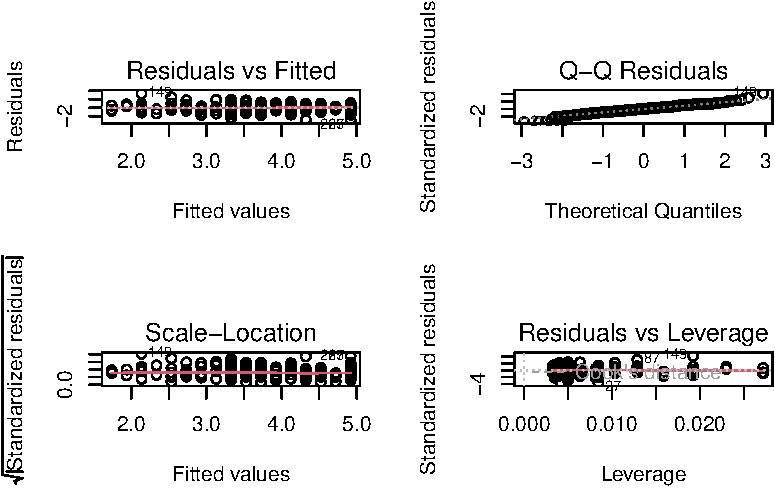
\includegraphics[width=1\textwidth,height=\textheight]{08-lm-continuous_files/figure-pdf/unnamed-chunk-29-1.pdf}
\end{center}

For more information on each of these plots, see this great resource by
\href{https://library.virginia.edu/data/articles/diagnostic-plots}{Kim
(2015)} via the University of Virginia, but we will break the key ones
down below.

\subsection{Checking linearity}\label{checking-linearity}

To isolate each plot, we can use the \texttt{which} argument. Plot 1 is
a residuals vs fitted plot and helps us check linearity by showing the
residuals on the y-axis and the fitted (predicted) values on the x-axis.

\begin{Shaded}
\begin{Highlighting}[]
\FunctionTok{plot}\NormalTok{(lm\_redistribution, }
     \AttributeTok{which =} \DecValTok{1}\NormalTok{)}
\end{Highlighting}
\end{Shaded}

\begin{center}
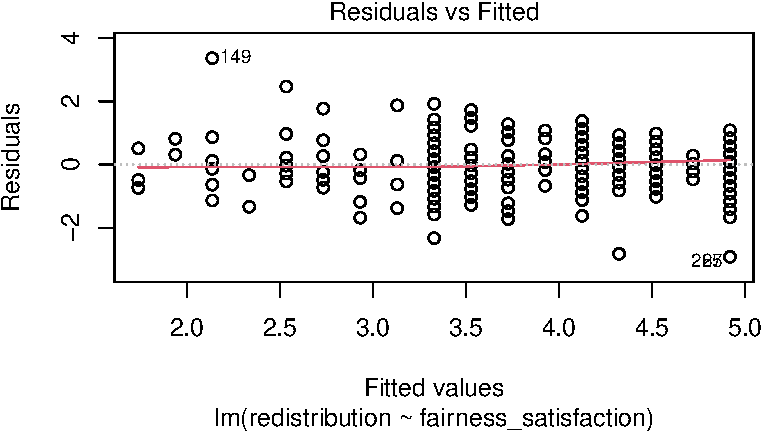
\includegraphics[width=1\textwidth,height=\textheight]{08-lm-continuous_files/figure-pdf/unnamed-chunk-30-1.pdf}
\end{center}

Here, you are looking out for a roughly flat horizontal red line. Common
patterns to look out for if there is a problem are when the line has an
obvious curve to look like a hump or several bends to look like an S.

The only downside to using diagnostic plots is it takes experience to
recognise when there is nothing wrong with a regression model compared
to when it violates the assumptions. It is easy to see a little
deviation and think there is some drastically wrong. Our advice is if
you squint and it looks fine, it is probably fine. You are looking for
clear and obvious deviations from what you expect and all the models we
use in Chapters 8 and 9 are intentionally fine to develop foundational
skills. In Chapter 11, we then introduce you to more problematic cases
and what your options are.

\begin{tcolorbox}[enhanced jigsaw, breakable, colframe=quarto-callout-important-color-frame, arc=.35mm, opacitybacktitle=0.6, titlerule=0mm, colbacktitle=quarto-callout-important-color!10!white, colback=white, toprule=.15mm, bottomtitle=1mm, toptitle=1mm, title=\textcolor{quarto-callout-important-color}{\faExclamation}\hspace{0.5em}{Error mode}, bottomrule=.15mm, rightrule=.15mm, leftrule=.75mm, coltitle=black, left=2mm, opacityback=0]

If you want to save these plots to add into a report, you might try
using \texttt{ggsave()} like we have covered in the data visualisation
chapters. However, it will not work as these plots have not been created
by ggplot2.

To save these plots, you can either right click and choose save as to
save on your computer. Alternatively, if they open in the Plots window,
you can click on Export and save them as an image or PDF to insert into
your documents.

\end{tcolorbox}

\subsection{Checking normality}\label{checking-normality}

Plot 2 is a qq-plot (quantile-quantile plot) and helps us check the
normality of the model residuals by showing the standardised residuals
on the y-axis and the theoretical quantiles on the x-axis. A common
misconception is your variables should all be normally distributed, but
it is actually the model residuals which should be normal.

\begin{Shaded}
\begin{Highlighting}[]
\FunctionTok{plot}\NormalTok{(lm\_redistribution, }
     \AttributeTok{which =} \DecValTok{2}\NormalTok{)}
\end{Highlighting}
\end{Shaded}

\begin{center}
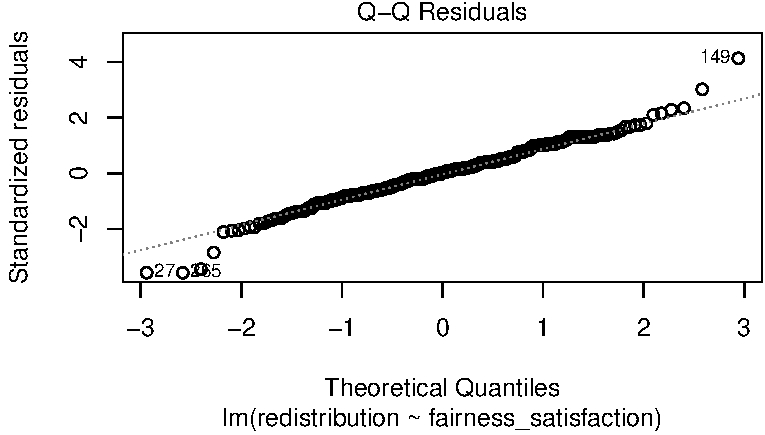
\includegraphics[width=1\textwidth,height=\textheight]{08-lm-continuous_files/figure-pdf/unnamed-chunk-31-1.pdf}
\end{center}

In this plot, you are looking for the data points to roughly follow the
dashed line. The idea is there should be a linear relationship between
the residuals and the values we would expect under a normal
distribution.

Like the other diagnostic plots, it is tempting to think there are
problems where there are none. The vast majority of the points here
follow the line nicely, but tail off a little at the extremes. It flags
the points with the largest deviations but there do not appear to be any
obvious problems.

When there are problems with normality, you are looking for obvious
deviations, like the points curving around in a banana shape, or snaking
around like an S.

\subsection{Checking homoscedasticity}\label{checking-homoscedasticity}

Plot 3 is a scale-location plot and helps us check homoscedasticity by
showing the square root of the standardised residuals on the y-axis and
the fitted values on the x-axis. Homoscedasticity is where the variance
of the residuals is approximately equal across the range of your
predictor(s).

\begin{Shaded}
\begin{Highlighting}[]
\FunctionTok{plot}\NormalTok{(lm\_redistribution, }
     \AttributeTok{which =} \DecValTok{3}\NormalTok{)}
\end{Highlighting}
\end{Shaded}

\begin{center}
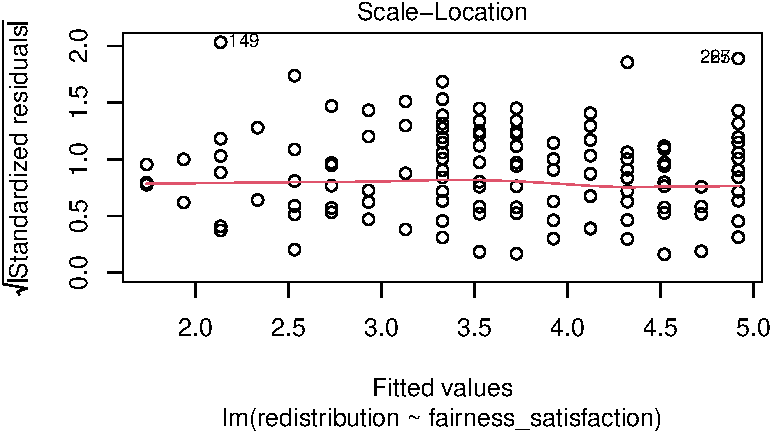
\includegraphics[width=1\textwidth,height=\textheight]{08-lm-continuous_files/figure-pdf/unnamed-chunk-32-1.pdf}
\end{center}

In this plot, you are looking out for a roughly random spread of points
as you move from one end of the x-axis to the other. The red line should
be roughly flat and horizontal.

When there is \emph{heteroscedasticity}, the characteristic patterns to
look out for are a kind of arrow shape where there is a wide spread of
points at one end and decreases to a denser range at the other end, or a
bow tie where there is a wide spread of points at each end and dense in
the middle.

\subsection{Checking influential
cases}\label{checking-influential-cases}

Finally, there are two main plots to help us identify influential cases.
You might have heard of the term outlier before and this is one way of
classifying data points that are different enough to the rest of the
data in a regression model. It is not strictly an assumption of linear
regression, but it can affect the other assumptions. Identifying
outliers is a complex decision and we will explore your options in the
course materials and Chapter 11 on data screening.

If you only run \texttt{plot(lm\_redistribution)} and cycle through the
plots, you do not see this version. This plot shows values of Cook's
distance for each observation in your data along the x-axis. Cook's
distance measures the influence of deleting a given observation, where
higher values mean deleting that observation results in a larger change
to the model estimates. There are different thresholds in the
literature, but estimates range from 1, 0.5, to 4/n.~We explore the
decision making around this and your options in Chapter 11.

\begin{Shaded}
\begin{Highlighting}[]
\FunctionTok{plot}\NormalTok{(lm\_redistribution, }
     \AttributeTok{which =} \DecValTok{4}\NormalTok{)}
\end{Highlighting}
\end{Shaded}

\begin{center}
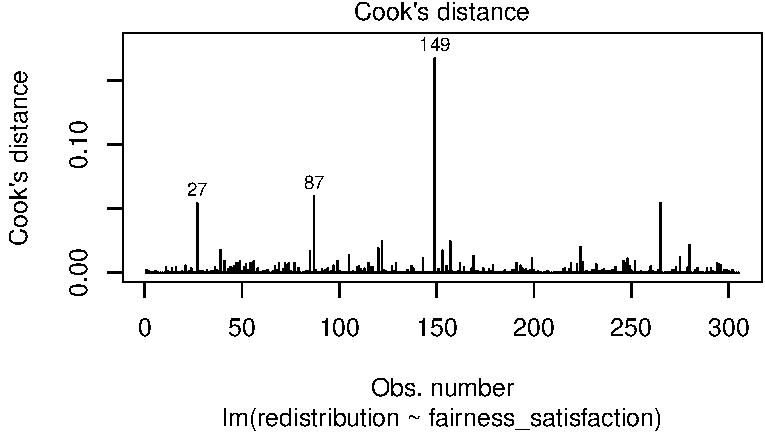
\includegraphics[width=1\textwidth,height=\textheight]{08-lm-continuous_files/figure-pdf/unnamed-chunk-33-1.pdf}
\end{center}

Finally, we get a residuals vs leverage plot to show influential cases
in a slightly different way. Instead of just the Cook's distance value
of each observation, it plots the standardised residuals against
leverage values.

\begin{Shaded}
\begin{Highlighting}[]
\FunctionTok{plot}\NormalTok{(lm\_redistribution, }
     \AttributeTok{which =} \DecValTok{5}\NormalTok{)}
\end{Highlighting}
\end{Shaded}

\begin{center}
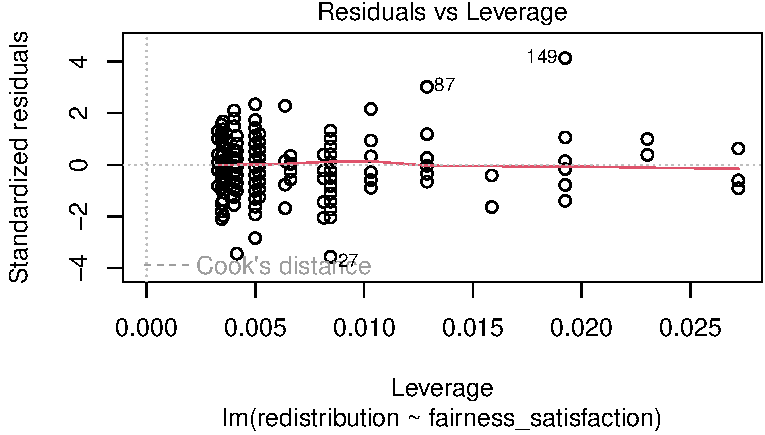
\includegraphics[width=1\textwidth,height=\textheight]{08-lm-continuous_files/figure-pdf/unnamed-chunk-34-1.pdf}
\end{center}

Influential points and potential outliers would have high leverage
values and the plot will show a threshold of Cook's distance as red
dashed lines. In this plot, they are not visible as there is no value
with a big enough leverage value, but you would be looking for data
points outside this threshold to identify influential values.

\subsection{Checking all the
assumptions}\label{checking-all-the-assumptions}

Now we have covered the individual diagnostic plots, there is a handy
function called \texttt{check\_model()} from the performance package.
This function reports all the diagnostic checks from \texttt{plot()},
but tidies up the presentation and has some useful reminders of what you
are looking for.

\begin{Shaded}
\begin{Highlighting}[]
\FunctionTok{check\_model}\NormalTok{(lm\_redistribution)}
\end{Highlighting}
\end{Shaded}

\begin{center}
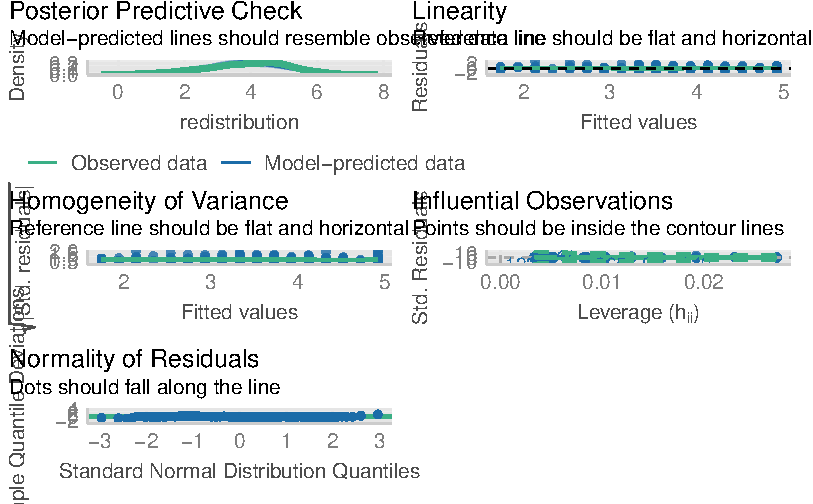
\includegraphics[width=1\textwidth,height=\textheight]{08-lm-continuous_files/figure-pdf/unnamed-chunk-35-1.pdf}
\end{center}

The key difference is you get a posterior predictive check (essentially
comparing values you observe compared to what your model predicts) and
the qq-plot for normality of residuals looks a little different. Instead
of a kind of angled line, the residuals are expressed as deviations
instead, so the points should be close to a flat horizontal line. This
version can make smaller deviations look worse, so keep in mind again
you are looking for clear deviations in the overall pattern.

\begin{tcolorbox}[enhanced jigsaw, breakable, colframe=quarto-callout-note-color-frame, arc=.35mm, opacitybacktitle=0.6, titlerule=0mm, colbacktitle=quarto-callout-note-color!10!white, colback=white, toprule=.15mm, bottomtitle=1mm, toptitle=1mm, title=\textcolor{quarto-callout-note-color}{\faInfo}\hspace{0.5em}{Note}, bottomrule=.15mm, rightrule=.15mm, leftrule=.75mm, coltitle=black, left=2mm, opacityback=0]

The performance version of the diagnostic plots are actually created
using ggplot2, so the function \texttt{ggsave()} would work here if you
need to save the plot to add into your report.

\end{tcolorbox}

\begin{tcolorbox}[enhanced jigsaw, breakable, colframe=quarto-callout-tip-color-frame, arc=.35mm, opacitybacktitle=0.6, titlerule=0mm, colbacktitle=quarto-callout-tip-color!10!white, colback=white, toprule=.15mm, bottomtitle=1mm, toptitle=1mm, title=\textcolor{quarto-callout-tip-color}{\faLightbulb}\hspace{0.5em}{Try this}, bottomrule=.15mm, rightrule=.15mm, leftrule=.75mm, coltitle=black, left=2mm, opacityback=0]

In activity 7, you should have calculated the relationship between age
and support for redistribution for your independent task. Using the
model object \texttt{lm\_age}, work through assumptions for simple
linear regression and make a note of whether you think it meets the
assumptions, or there might be any problems. Some of the assumptions you
consider what you know about the design, while others you need the
diagnostic plots.

\begin{enumerate}
\def\labelenumi{\arabic{enumi}.}
\item
  The outcome is interval/ratio level data.
\item
  The predictor variable is interval/ratio or categorical (with two
  levels at a time).
\item
  All values of the outcome variable are independent (i.e., each score
  should come from a different participant/observation).
\item
  The predictors have non-zero variance.
\item
  The relationship between the outcome and predictor is linear.
\item
  The residuals should be normally distributed.
\item
  There should be homoscedasticity.
\end{enumerate}

\end{tcolorbox}

\begin{tcolorbox}[enhanced jigsaw, breakable, colframe=quarto-callout-caution-color-frame, arc=.35mm, opacitybacktitle=0.6, titlerule=0mm, colbacktitle=quarto-callout-caution-color!10!white, colback=white, toprule=.15mm, bottomtitle=1mm, toptitle=1mm, title=\textcolor{quarto-callout-caution-color}{\faFire}\hspace{0.5em}{Show me the solution}, bottomrule=.15mm, rightrule=.15mm, leftrule=.75mm, coltitle=black, left=2mm, opacityback=0]

\begin{enumerate}
\def\labelenumi{\arabic{enumi}.}
\tightlist
\item
  The outcome is interval/ratio level data.
\end{enumerate}

\textbf{There is a debate here we cover in the course materials, but
there is an argument you can treat the average of multiple Likert items
as interval, but you need to be careful.}

\begin{enumerate}
\def\labelenumi{\arabic{enumi}.}
\setcounter{enumi}{1}
\tightlist
\item
  The predictor variable is interval/ratio or categorical (with two
  levels at a time).
\end{enumerate}

\textbf{Our predictor age is nicely ratio.}

\begin{enumerate}
\def\labelenumi{\arabic{enumi}.}
\setcounter{enumi}{2}
\tightlist
\item
  All values of the outcome variable are independent (i.e., each score
  should come from a different participant/observation).
\end{enumerate}

\textbf{You need to know this from the design / data collection, but it
appears to be the case in this study.}

\begin{enumerate}
\def\labelenumi{\arabic{enumi}.}
\setcounter{enumi}{3}
\tightlist
\item
  The predictors have non-zero variance.
\end{enumerate}

\textbf{There are a range of ages in the data.}

\begin{enumerate}
\def\labelenumi{\arabic{enumi}.}
\setcounter{enumi}{4}
\tightlist
\item
  The relationship between the outcome and predictor is linear.
\end{enumerate}

\textbf{Looking at the first plot, the red line is pretty flat and
horizontal, so we are happy with this.}

\begin{Shaded}
\begin{Highlighting}[]
\FunctionTok{plot}\NormalTok{(lm\_age, }\AttributeTok{which =} \DecValTok{1}\NormalTok{)}
\end{Highlighting}
\end{Shaded}

\begin{center}
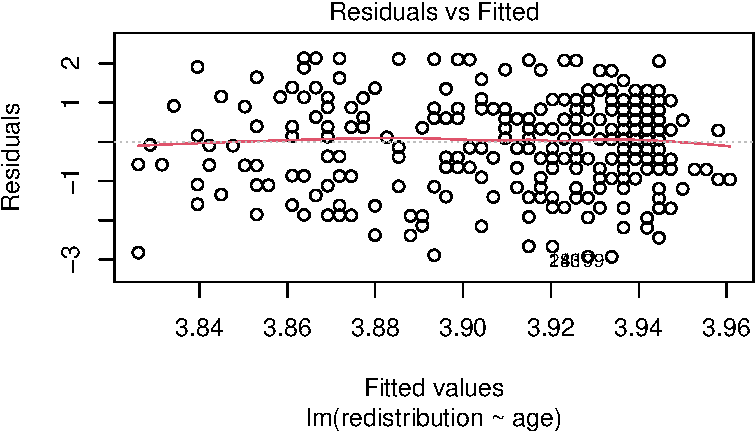
\includegraphics[width=1\textwidth,height=\textheight]{08-lm-continuous_files/figure-pdf/unnamed-chunk-36-1.pdf}
\end{center}

\begin{enumerate}
\def\labelenumi{\arabic{enumi}.}
\setcounter{enumi}{5}
\tightlist
\item
  The residuals should be normally distributed.
\end{enumerate}

\textbf{The qq-plot is fine for the vast majority of the range. We just
have a few deviations in the extreme ends of the x-axis, but this is a
byproduct of using a scale score as our outcome as responses cannot go
beyond 1-6.}

\begin{Shaded}
\begin{Highlighting}[]
\FunctionTok{plot}\NormalTok{(lm\_age, }\AttributeTok{which =} \DecValTok{2}\NormalTok{)}
\end{Highlighting}
\end{Shaded}

\begin{center}
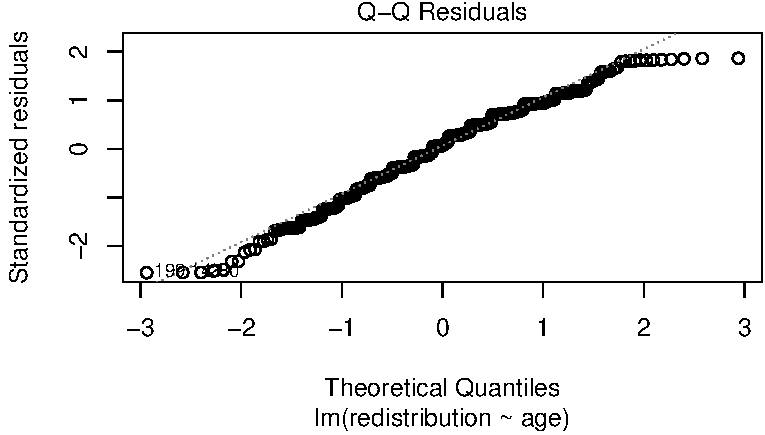
\includegraphics[width=1\textwidth,height=\textheight]{08-lm-continuous_files/figure-pdf/unnamed-chunk-37-1.pdf}
\end{center}

\begin{enumerate}
\def\labelenumi{\arabic{enumi}.}
\setcounter{enumi}{6}
\tightlist
\item
  There should be homoscedasticity.
\end{enumerate}

\textbf{The red line is pretty flat and it looks like there is a fairly
even range of values across the x-axis range.}

\begin{Shaded}
\begin{Highlighting}[]
\FunctionTok{plot}\NormalTok{(lm\_age, }\AttributeTok{which =} \DecValTok{3}\NormalTok{)}
\end{Highlighting}
\end{Shaded}

\begin{center}
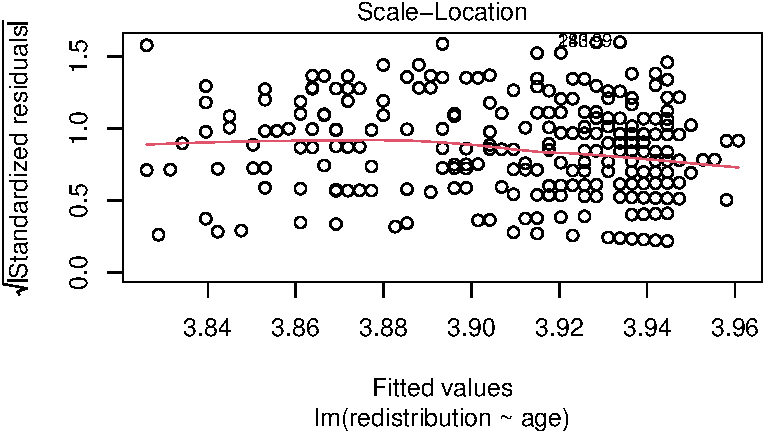
\includegraphics[width=1\textwidth,height=\textheight]{08-lm-continuous_files/figure-pdf/unnamed-chunk-38-1.pdf}
\end{center}

All in all, there do not appear to be any issues with the assumptions
here.

\end{tcolorbox}

\section{Reporting your results}\label{reporting-your-results}

Now we have some results to go with, there are a few recommendations on
how to communicate that information. In psychology (and other
disciplines), we tend to follow the American Psychological Association
(APA) formatting guidelines as they provide a comprehensive standardised
style to make sure information is being reported as easily digestible
and consistent as possible. You can see
\href{https://apastyle.apa.org/instructional-aids/numbers-statistics-guide.pdf}{this
PDF online} for a little cheat sheet for numbers and statistics, but we
will outline some key principles to ensure you provide your reader with
enough information.

\begin{enumerate}
\def\labelenumi{\arabic{enumi}.}
\item
  Explain to the reader what your linear regression model was. For
  example, what was your outcome and predictor variable?
\item
  Report descriptive statistics to help contextualise your findings. For
  example, the mean/standard deviation for your outcome and continuous
  predictor.
\item
  Provide an appropriate data visualisation to help communciate key
  patterns to the reader. For example, a scatterplot for the
  relationship between your outcome and predictor.
\item
  Report all three key inferential statistics concepts for the
  coefficient: the slope, the confidence interval around your slope, and
  the \emph{p}-value for hypothesis testing. When you have one predictor
  in simple linear regression, you typically focus on the slope as your
  key effect size that helps address your research question and
  hypothesis. APA style rounds numbers to 2 decimal places when numbers
  can be bigger than 1, and 3 decimals with no leading zero when it
  cannot be bigger than 1. When you report the unstandardised slope, you
  use the symbol \(b_1\) but for the standardised slope, you use Beta
  instead \(\beta_1\).
\item
  Provide an overview of the model fit statistics for whether your model
  explained a significant amount of variance in your outcome. Remember:
  the \emph{p}-value for your model will be the same as for the slope in
  simple linear regression.
\end{enumerate}

For our main example, we could summarise the findings as:

``Our research question was: is there a relationship between support for
wealth redistribution and fairness and satisfaction with the current
system? To test this, we applied simple linear regression using fairness
and satisfaction as a predictor and support for wealth redistribution as
our outcome. Figure 1 shows a scatterplot of the relationship.

\begin{center}
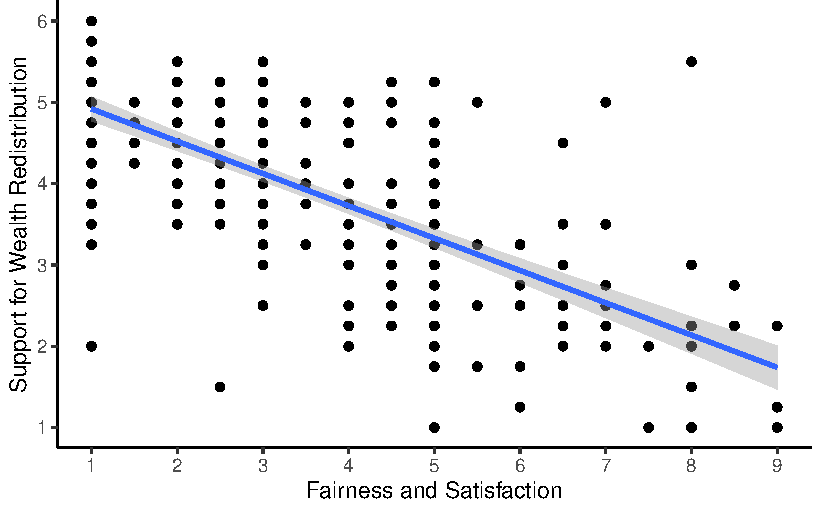
\includegraphics[width=1\textwidth,height=\textheight]{08-lm-continuous_files/figure-pdf/unnamed-chunk-39-1.pdf}
\end{center}

Our model explained a statistically significant amount of variance in
our outcome (adjusted \(R^2\) = .489, F(1, 303) = 291.70, \emph{p}
\textless{} .001). Fairness and satisfaction was a negative predictor,
where for every 1-unit increase we expect support for redistribution to
decrease by 0.40 (\(b_1 = -0.40\), 95\% CI = {[}-0.44, -0.35{]},
\emph{p} \textless{} .001).''

Note: we have not included an APA formatted Figure title here as it is
not easy to format in our book, so refer to the course materials for
guidance.

\subsection{Formatting your results
reproducibly}\label{formatting-your-results-reproducibly}

After the correlation example, we can also make regression models
reproducible to add into your reports. For regression models, the first
step is saving your model as an object \emph{before} you apply the
\texttt{summary()} function. We created this in activity 6, but as a
reminder:

\begin{Shaded}
\begin{Highlighting}[]
\NormalTok{lm\_redistribution }\OtherTok{\textless{}{-}} \FunctionTok{lm}\NormalTok{(redistribution }\SpecialCharTok{\textasciitilde{}}\NormalTok{ fairness\_satisfaction,}
                        \AttributeTok{data =}\NormalTok{ dawtry\_clean)}
\end{Highlighting}
\end{Shaded}

To make the reporting flexible, we then separate the model into two
components: the overall model and the slope. For the overall model, you
must save the reporting function first.

\begin{Shaded}
\begin{Highlighting}[]
\NormalTok{report\_regression\_model }\OtherTok{\textless{}{-}} \ControlFlowTok{function}\NormalTok{(regression\_object)\{}
  \CommentTok{\# This function will only work for lm() objects}
  \CommentTok{\# Step 1 = apply the summary function so we have both objects}
\NormalTok{  model\_summary }\OtherTok{\textless{}{-}} \FunctionTok{summary}\NormalTok{(regression\_object)}
  \CommentTok{\# Step 2 = save all the numbers with formatting }
  \CommentTok{\# Save adjusted R2 with any trailing zeroes}
\NormalTok{  adj\_r2 }\OtherTok{\textless{}{-}} \FunctionTok{sprintf}\NormalTok{(}\StringTok{"\%.3f"}\NormalTok{, }\FunctionTok{round}\NormalTok{(model\_summary}\SpecialCharTok{$}\NormalTok{adj.r.squared, }\DecValTok{3}\NormalTok{))}
  \CommentTok{\# save model degrees of freedom}
\NormalTok{  df1 }\OtherTok{\textless{}{-}}\NormalTok{ model\_summary}\SpecialCharTok{$}\NormalTok{df[}\DecValTok{1}\NormalTok{]}
  \CommentTok{\# save residual degrees of freedom}
\NormalTok{  df2 }\OtherTok{\textless{}{-}}\NormalTok{ model\_summary}\SpecialCharTok{$}\NormalTok{df[}\DecValTok{2}\NormalTok{]}
  \CommentTok{\# save F rounded to 2 decimals with any trailing zeroes}
\NormalTok{  Fval }\OtherTok{\textless{}{-}} \FunctionTok{sprintf}\NormalTok{(}\StringTok{"\%.2f"}\NormalTok{, }\FunctionTok{round}\NormalTok{(model\_summary}\SpecialCharTok{$}\NormalTok{fstatistic, }\DecValTok{2}\NormalTok{))[}\DecValTok{1}\NormalTok{]}
  \CommentTok{\# save p value with formatting if less than .001}
\NormalTok{  pval }\OtherTok{\textless{}{-}} \FunctionTok{anova}\NormalTok{(regression\_object)}\SpecialCharTok{$}\StringTok{\textasciigrave{}}\AttributeTok{Pr(\textgreater{}F)}\StringTok{\textasciigrave{}}\NormalTok{[}\DecValTok{1}\NormalTok{]}
  \ControlFlowTok{if}\NormalTok{ (pval }\SpecialCharTok{\textgreater{}=} \FloatTok{0.001}\NormalTok{)\{}
\NormalTok{    pval }\OtherTok{\textless{}{-}} \FunctionTok{str\_sub}\NormalTok{(}\FunctionTok{as.character}\NormalTok{(pval), }\DecValTok{2}\NormalTok{, }\DecValTok{5}\NormalTok{)}
\NormalTok{    pval }\OtherTok{\textless{}{-}}  \FunctionTok{paste0}\NormalTok{(}\StringTok{", *p* = "}\NormalTok{, pval)}
  \CommentTok{\# If p \textless{} .001, manually format as p \textless{} .001}
\NormalTok{  \} }\ControlFlowTok{else} \ControlFlowTok{if}\NormalTok{ (pval }\SpecialCharTok{\textless{}} \FloatTok{0.001}\NormalTok{)\{}
\NormalTok{    pval }\OtherTok{\textless{}{-}} \StringTok{", *p* \textless{} .001"}
\NormalTok{  \}}

  \CommentTok{\# Step 3 = add them together in APA format}
\NormalTok{  output }\OtherTok{\textless{}{-}} \FunctionTok{paste0}\NormalTok{(}\StringTok{"adjusted $R\^{}2$ = "}\NormalTok{,}
\NormalTok{                   adj\_r2,}
                   \StringTok{", "}\NormalTok{,}
                   \StringTok{"F("}\NormalTok{, df1, }\StringTok{", "}\NormalTok{, df2, }\StringTok{") = "}\NormalTok{, Fval,}
\NormalTok{                   pval)}
  
  \FunctionTok{return}\NormalTok{(output)}
\NormalTok{\}}
\end{Highlighting}
\end{Shaded}

Then you can run the function on your regression model.

\begin{Shaded}
\begin{Highlighting}[]
\FunctionTok{report\_regression\_model}\NormalTok{(lm\_redistribution)}
\end{Highlighting}
\end{Shaded}

\begin{verbatim}
[1] "adjusted $R^2$ = 0.489, F(2, 303) = 291.67, *p* < .001"
\end{verbatim}

For the slope, there is a separate reporting function.

\begin{Shaded}
\begin{Highlighting}[]
\NormalTok{report\_regression\_slope }\OtherTok{\textless{}{-}} \ControlFlowTok{function}\NormalTok{(regression\_object)\{}
  \CommentTok{\# This function will only work for lm() objects}
  \CommentTok{\# Step 1 = apply the summary function so we have both objects}
\NormalTok{  model\_summary }\OtherTok{\textless{}{-}} \FunctionTok{summary}\NormalTok{(regression\_object)}
  \CommentTok{\# Step 2 = save all the numbers with formatting }
  \CommentTok{\# $b\_1 = {-}0.40$, 95\% CI = [{-}0.44, {-}0.35], *p* \textless{} .001)}
  \CommentTok{\# Save slope with any trailing zeroes}
\NormalTok{  b\_1 }\OtherTok{\textless{}{-}} \FunctionTok{sprintf}\NormalTok{(}\StringTok{"\%.2f"}\NormalTok{, }\FunctionTok{round}\NormalTok{(model\_summary}\SpecialCharTok{$}\NormalTok{coefficients[}\DecValTok{2}\NormalTok{, }\DecValTok{1}\NormalTok{], }\DecValTok{2}\NormalTok{))}
  \CommentTok{\# save p value with formatting if less than .001}
\NormalTok{  pval }\OtherTok{\textless{}{-}}\NormalTok{ model\_summary}\SpecialCharTok{$}\NormalTok{coefficients[}\DecValTok{2}\NormalTok{, }\DecValTok{4}\NormalTok{]}
  \ControlFlowTok{if}\NormalTok{ (pval }\SpecialCharTok{\textgreater{}=} \FloatTok{0.001}\NormalTok{)\{}
\NormalTok{    pval }\OtherTok{\textless{}{-}} \FunctionTok{str\_sub}\NormalTok{(}\FunctionTok{as.character}\NormalTok{(pval), }\DecValTok{2}\NormalTok{, }\DecValTok{5}\NormalTok{)}
\NormalTok{    pval }\OtherTok{\textless{}{-}}  \FunctionTok{paste0}\NormalTok{(}\StringTok{", *p* = "}\NormalTok{, pval)}
  \CommentTok{\# If p \textless{} .001, manually format as p \textless{} .001}
\NormalTok{  \} }\ControlFlowTok{else} \ControlFlowTok{if}\NormalTok{ (pval }\SpecialCharTok{\textless{}} \FloatTok{0.001}\NormalTok{)\{}
\NormalTok{    pval }\OtherTok{\textless{}{-}} \StringTok{", *p* \textless{} .001"}
\NormalTok{  \}}
  \CommentTok{\# save lower 95\% CI}
\NormalTok{  lower\_CI }\OtherTok{\textless{}{-}} \FunctionTok{round}\NormalTok{(}\FunctionTok{confint}\NormalTok{(regression\_object)[}\DecValTok{2}\NormalTok{, }\DecValTok{1}\NormalTok{], }\DecValTok{2}\NormalTok{)}
  \CommentTok{\# save lower 95\% CI}
\NormalTok{  upper\_CI }\OtherTok{\textless{}{-}} \FunctionTok{round}\NormalTok{(}\FunctionTok{confint}\NormalTok{(regression\_object)[}\DecValTok{2}\NormalTok{, }\DecValTok{2}\NormalTok{], }\DecValTok{2}\NormalTok{)}
  \CommentTok{\# Switch CIs depending on sign }
\NormalTok{  b1\_CI }\OtherTok{\textless{}{-}} \FunctionTok{ifelse}\NormalTok{(b\_1 }\SpecialCharTok{\textgreater{}} \DecValTok{0}\NormalTok{,}
                 \FunctionTok{paste0}\NormalTok{(lower\_CI, }\StringTok{", "}\NormalTok{, upper\_CI),}
                 \FunctionTok{paste0}\NormalTok{(upper\_CI, }\StringTok{", "}\NormalTok{, lower\_CI))}
  
  \CommentTok{\# Step 3 = add them together in APA format}
\NormalTok{  output }\OtherTok{\textless{}{-}} \FunctionTok{paste0}\NormalTok{(}\StringTok{"$b\_1$ = "}\NormalTok{,}
\NormalTok{                   b\_1,}
                   \StringTok{", 95\% CI = ["}\NormalTok{, b1\_CI, }\StringTok{"]"}\NormalTok{,}
\NormalTok{                   pval)}
  
  \FunctionTok{return}\NormalTok{(output)}
\NormalTok{\}}
\end{Highlighting}
\end{Shaded}

Then you can run the function on your regression model.

\begin{Shaded}
\begin{Highlighting}[]
\FunctionTok{report\_regression\_slope}\NormalTok{(lm\_redistribution)}
\end{Highlighting}
\end{Shaded}

\begin{verbatim}
[1] "$b_1$ = -0.40, 95% CI = [-0.35, -0.44], *p* < .001"
\end{verbatim}

\section{Test Yourself}\label{test-yourself-6}

To end the chapter, we have some knowledge check questions to test your
understanding of the concepts we covered in the chapter. We then have
some error mode tasks to see if you can find the solution to some common
errors in the concepts we covered in this chapter.

\subsection{Knowledge check}\label{knowledge-check-7}

For this chapter's knowledge check section, we have something a little
different. Instead of purely conceptual questions about functions, we
have another example of linear regression from Dawtry et al. (2015).
Feel free to create this model yourself, but we will show you some
output and ask you questions based on it.

For this model, we focus on the two variables estimated population
inequality index (\texttt{Population\_Inequality\_Gini\_Index}) and
support for wealth redistribution (\texttt{redistribution}). Check back
to the code book in \hyperref[08-explore]{Activity 2} if you need a
reminder of what the variables mean.

\textbf{Question 1}. In the scatterplot of the relationship below, this
shows a negative relationship between the inequality index and support
for redistribution: TRUE / FALSE.

\begin{center}
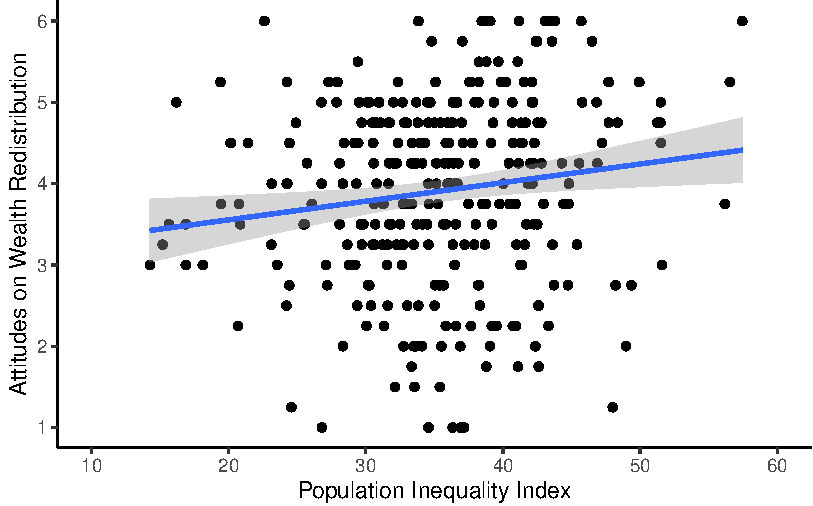
\includegraphics[width=1\textwidth,height=\textheight]{08-lm-continuous_files/figure-pdf/unnamed-chunk-45-1.pdf}
\end{center}

\textbf{Question 2} For the next few questions, we have the output from
a linear regression model and we would like you to interpret it.

\begin{verbatim}

Call:
lm(formula = redistribution ~ Population_Inequality_Gini_Index, 
    data = dawtry_clean)

Residuals:
    Min      1Q  Median      3Q     Max 
-2.9478 -0.6384  0.1389  0.8511  2.3854 

Coefficients:
                                 Estimate Std. Error t value Pr(>|t|)    
(Intercept)                      3.097452   0.316914   9.774  < 2e-16 ***
Population_Inequality_Gini_Index 0.022879   0.008734   2.619  0.00925 ** 
---
Signif. codes:  0 '***' 0.001 '**' 0.01 '*' 0.05 '.' 0.1 ' ' 1

Residual standard error: 1.139 on 303 degrees of freedom
Multiple R-squared:  0.02214,   Adjusted R-squared:  0.01892 
F-statistic: 6.861 on 1 and 303 DF,  p-value: 0.009251
\end{verbatim}

The outcome variable in this model is

\begin{itemize}
\tightlist
\item
  \begin{enumerate}
  \def\labelenumi{(\Alph{enumi})}
  \tightlist
  \item
    Attitudes on Wealth Redistribution\\
  \end{enumerate}
\item
  \begin{enumerate}
  \def\labelenumi{(\Alph{enumi})}
  \setcounter{enumi}{1}
  \tightlist
  \item
    Population Inequality Index
  \end{enumerate}
\end{itemize}

and the predictor variable is

\begin{itemize}
\tightlist
\item
  \begin{enumerate}
  \def\labelenumi{(\Alph{enumi})}
  \tightlist
  \item
    Attitudes on Wealth Redistribution\\
  \end{enumerate}
\item
  \begin{enumerate}
  \def\labelenumi{(\Alph{enumi})}
  \setcounter{enumi}{1}
  \tightlist
  \item
    Population Inequality Index
  \end{enumerate}
\end{itemize}

.

\textbf{Question 3} Rounded to 2 decimals, when the predictor is 0, we
predict a value of \_\_\_ for our outcome variable.

\textbf{Question 4} The predictor is

\begin{itemize}
\tightlist
\item
  \begin{enumerate}
  \def\labelenumi{(\Alph{enumi})}
  \tightlist
  \item
    significant\\
  \end{enumerate}
\item
  \begin{enumerate}
  \def\labelenumi{(\Alph{enumi})}
  \setcounter{enumi}{1}
  \tightlist
  \item
    non-significant
  \end{enumerate}
\end{itemize}

with a \emph{p}-value of \_\_\_\_\_.

\textbf{Question 5} The predictor is

\begin{itemize}
\tightlist
\item
  \begin{enumerate}
  \def\labelenumi{(\Alph{enumi})}
  \tightlist
  \item
    positive\\
  \end{enumerate}
\item
  \begin{enumerate}
  \def\labelenumi{(\Alph{enumi})}
  \setcounter{enumi}{1}
  \tightlist
  \item
    negative
  \end{enumerate}
\end{itemize}

, where we expect for every 1-unit increase in the predictor a \_\_\_\_
-unit

\begin{itemize}
\tightlist
\item
  \begin{enumerate}
  \def\labelenumi{(\Alph{enumi})}
  \tightlist
  \item
    increase\\
  \end{enumerate}
\item
  \begin{enumerate}
  \def\labelenumi{(\Alph{enumi})}
  \setcounter{enumi}{1}
  \tightlist
  \item
    decrease
  \end{enumerate}
\end{itemize}

in the outcome.

\subsection{Error mode}\label{error-mode-19}

The following questions are designed to introduce you to making and
fixing errors. For this topic, we focus on simple linear regression
between two continuous variables. There are not many outright errors
that people make here, more misspecifications that are not doing what
you think they are doing.

Create and save a new R Markdown file for these activities. Delete the
example code, so your file is blank from line 10. Create a new code
chunk to load tidyverse and wrangle the data files:

\begin{Shaded}
\begin{Highlighting}[]
\CommentTok{\# Load the packages below}
\FunctionTok{library}\NormalTok{(tidyverse)}
\FunctionTok{library}\NormalTok{(effectsize)}
\FunctionTok{library}\NormalTok{(correlation)}
\FunctionTok{library}\NormalTok{(performance)}

\CommentTok{\# Load the data file}
\CommentTok{\# This should be the Dawtry\_2015.csv file }
\NormalTok{dawtry\_data }\OtherTok{\textless{}{-}} \FunctionTok{read\_csv}\NormalTok{(}\StringTok{"data/Dawtry\_2015.csv"}\NormalTok{)}

\CommentTok{\# Reverse code redist2 and redist4}
\NormalTok{dawtry\_data }\OtherTok{\textless{}{-}}\NormalTok{ dawtry\_data }\SpecialCharTok{\%\textgreater{}\%}
  \FunctionTok{mutate}\NormalTok{(}\AttributeTok{redist2\_R =} \DecValTok{7} \SpecialCharTok{{-}}\NormalTok{ redist2,}
         \AttributeTok{redist4\_R =} \DecValTok{7} \SpecialCharTok{{-}}\NormalTok{ redist4)}

\CommentTok{\# calculate mean fairness and satisfaction score  }
\NormalTok{fairness\_satisfaction }\OtherTok{\textless{}{-}}\NormalTok{ dawtry\_data }\SpecialCharTok{\%\textgreater{}\%} 
  \FunctionTok{pivot\_longer}\NormalTok{(}\AttributeTok{cols =}\NormalTok{ fairness}\SpecialCharTok{:}\NormalTok{satisfaction, }
               \AttributeTok{names\_to =} \StringTok{"Items"}\NormalTok{, }
               \AttributeTok{values\_to =} \StringTok{"Response"}\NormalTok{) }\SpecialCharTok{\%\textgreater{}\%} 
  \FunctionTok{group\_by}\NormalTok{(PS) }\SpecialCharTok{\%\textgreater{}\%} 
  \FunctionTok{summarise}\NormalTok{(}\AttributeTok{fairness\_satisfaction =} \FunctionTok{mean}\NormalTok{(Response)) }\SpecialCharTok{\%\textgreater{}\%} 
  \FunctionTok{ungroup}\NormalTok{()}

\CommentTok{\# calculate mean wealth redistribution score  }
\NormalTok{redistribution }\OtherTok{\textless{}{-}}\NormalTok{ dawtry\_data }\SpecialCharTok{\%\textgreater{}\%} 
  \FunctionTok{pivot\_longer}\NormalTok{(}\AttributeTok{cols =} \FunctionTok{c}\NormalTok{(redist1, redist2\_R, redist3, redist4\_R), }
               \AttributeTok{names\_to =} \StringTok{"Items"}\NormalTok{, }
               \AttributeTok{values\_to =} \StringTok{"Response"}\NormalTok{) }\SpecialCharTok{\%\textgreater{}\%} 
  \FunctionTok{group\_by}\NormalTok{(PS) }\SpecialCharTok{\%\textgreater{}\%} 
  \FunctionTok{summarise}\NormalTok{(}\AttributeTok{redistribution =} \FunctionTok{mean}\NormalTok{(Response)) }\SpecialCharTok{\%\textgreater{}\%} 
  \FunctionTok{ungroup}\NormalTok{()}

\CommentTok{\# join data and select columns for focus}
\NormalTok{dawtry\_clean }\OtherTok{\textless{}{-}}\NormalTok{ dawtry\_data }\SpecialCharTok{\%\textgreater{}\%} 
  \FunctionTok{inner\_join}\NormalTok{(fairness\_satisfaction, }\AttributeTok{by =} \StringTok{"PS"}\NormalTok{) }\SpecialCharTok{\%\textgreater{}\%} 
  \FunctionTok{inner\_join}\NormalTok{(redistribution, }\AttributeTok{by =} \StringTok{"PS"}\NormalTok{) }\SpecialCharTok{\%\textgreater{}\%} 
  \FunctionTok{select}\NormalTok{(PS, Household\_Income}\SpecialCharTok{:}\NormalTok{redistribution, }\SpecialCharTok{{-}}\NormalTok{redist2\_R, }\SpecialCharTok{{-}}\NormalTok{redist4\_R)}
\end{Highlighting}
\end{Shaded}

Below, we have several variations of a misspecification. Copy and paste
them into your R Markdown file below the code chunk to wrangle the data.
Once you have copied the activities, click knit and look at the output
you receive. See if you can identify the mistake and fix it before
checking the answer.

\textbf{Question 6}. Copy the following code chunk into your R Markdown
file and press knit. We want to create a simple linear regression model
to specify \texttt{fairness\_satisfaction} as our outcome variable and
\texttt{Political\_Preference} as our predictor. Have we expressed that
accurately?

\begin{Shaded}
\begin{Highlighting}[]
\InformationTok{\textasciigrave{}\textasciigrave{}\textasciigrave{}\{r\}}
\InformationTok{lm\_fairness \textless{}{-} lm(Political\_Preference \textasciitilde{} fairness\_satisfaction,}
\InformationTok{                        data = dawtry\_clean)}

\InformationTok{summary(lm\_fairness)}
\InformationTok{\textasciigrave{}\textasciigrave{}\textasciigrave{}}
\end{Highlighting}
\end{Shaded}

\begin{tcolorbox}[enhanced jigsaw, breakable, colframe=quarto-callout-caution-color-frame, arc=.35mm, opacitybacktitle=0.6, titlerule=0mm, colbacktitle=quarto-callout-caution-color!10!white, colback=white, toprule=.15mm, bottomtitle=1mm, toptitle=1mm, title=\textcolor{quarto-callout-caution-color}{\faFire}\hspace{0.5em}{Explain the solution}, bottomrule=.15mm, rightrule=.15mm, leftrule=.75mm, coltitle=black, left=2mm, opacityback=0]

In this example, we mixed up the variables. The formula in \texttt{lm()}
has the form \texttt{outcome\ \textasciitilde{}\ predictor}, so we mixed
up the order. In simple linear regression, it makes no difference to the
slope, but it is important to be able to express your model accurately
and it would make a difference once you scale up to multiple linear
regression.

\begin{Shaded}
\begin{Highlighting}[]
\NormalTok{lm\_fairness }\OtherTok{\textless{}{-}} \FunctionTok{lm}\NormalTok{(fairness\_satisfaction }\SpecialCharTok{\textasciitilde{}}\NormalTok{ Political\_Preference,}
                        \AttributeTok{data =}\NormalTok{ dawtry\_clean)}
                        
\FunctionTok{summary}\NormalTok{(lm\_fairness)}
\end{Highlighting}
\end{Shaded}

\end{tcolorbox}

\textbf{Question 7}. Copy the following code chunk into your R Markdown
file and press knit. We want to standardise the outcome and predictors,
so that we get the intercept and slope estimates in standard deviations.
Have we expressed that accurately?

\begin{Shaded}
\begin{Highlighting}[]
\InformationTok{\textasciigrave{}\textasciigrave{}\textasciigrave{}\{r\}}
\InformationTok{dawtry\_clean \textless{}{-} dawtry\_clean \%\textgreater{}\% }
\InformationTok{  mutate(fairness\_std = (fairness\_satisfaction {-} mean(fairness\_satisfaction)) / sd(fairness\_satisfaction))}

\InformationTok{lm\_fairness \textless{}{-} lm(fairness\_std \textasciitilde{} Political\_Preference,}
\InformationTok{                        data = dawtry\_clean)}
\InformationTok{                        }
\InformationTok{summary(lm\_fairness)}
\InformationTok{\textasciigrave{}\textasciigrave{}\textasciigrave{}}
\end{Highlighting}
\end{Shaded}

\begin{tcolorbox}[enhanced jigsaw, breakable, colframe=quarto-callout-caution-color-frame, arc=.35mm, opacitybacktitle=0.6, titlerule=0mm, colbacktitle=quarto-callout-caution-color!10!white, colback=white, toprule=.15mm, bottomtitle=1mm, toptitle=1mm, title=\textcolor{quarto-callout-caution-color}{\faFire}\hspace{0.5em}{Explain the solution}, bottomrule=.15mm, rightrule=.15mm, leftrule=.75mm, coltitle=black, left=2mm, opacityback=0]

In this example, we only standardised the outcome. When we standardise
predictors, we must standardise both the outcome and predictor so they
are expressed in standard deviations. It is just when we center, we only
center the predictor.

\begin{Shaded}
\begin{Highlighting}[]
\NormalTok{dawtry\_clean }\OtherTok{\textless{}{-}}\NormalTok{ dawtry\_clean }\SpecialCharTok{\%\textgreater{}\%} 
  \FunctionTok{mutate}\NormalTok{(}\AttributeTok{fairness\_std =}\NormalTok{ (fairness\_satisfaction }\SpecialCharTok{{-}} \FunctionTok{mean}\NormalTok{(fairness\_satisfaction)) }\SpecialCharTok{/} \FunctionTok{sd}\NormalTok{(fairness\_satisfaction),}
         \AttributeTok{Political\_std =}\NormalTok{ (Political\_Preference }\SpecialCharTok{{-}} \FunctionTok{mean}\NormalTok{(Political\_Preference, }\AttributeTok{na.rm =} \ConstantTok{TRUE}\NormalTok{)) }\SpecialCharTok{/} \FunctionTok{sd}\NormalTok{(Political\_Preference, }\AttributeTok{na.rm =} \ConstantTok{TRUE}\NormalTok{))}

\NormalTok{lm\_fairness }\OtherTok{\textless{}{-}} \FunctionTok{lm}\NormalTok{(fairness\_std }\SpecialCharTok{\textasciitilde{}}\NormalTok{ Political\_std,}
                        \AttributeTok{data =}\NormalTok{ dawtry\_clean)}
                        
\FunctionTok{summary}\NormalTok{(lm\_fairness)}
\end{Highlighting}
\end{Shaded}

\end{tcolorbox}

\section{Words from this Chapter}\label{words-from-this-chapter-7}

Below you will find a list of words that were used in this chapter that
might be new to you in case it helps to have somewhere to refer back to
what they mean. The links in this table take you to the entry for the
words in the \href{https://psyteachr.github.io/glossary/}{PsyTeachR
Glossary}. Note that the Glossary is written by numerous members of the
team and as such may use slightly different terminology from that shown
in the chapter.

\begin{longtable}[]{@{}
  >{\raggedright\arraybackslash}p{(\columnwidth - 2\tabcolsep) * \real{0.1933}}
  >{\raggedright\arraybackslash}p{(\columnwidth - 2\tabcolsep) * \real{0.8067}}@{}}
\toprule\noalign{}
\begin{minipage}[b]{\linewidth}\raggedright
term
\end{minipage} & \begin{minipage}[b]{\linewidth}\raggedright
definition
\end{minipage} \\
\midrule\noalign{}
\endhead
\bottomrule\noalign{}
\endlastfoot
\href{https://psyteachr.github.io/glossary/c\#centered-predictors}{centered-predictors}
& Usually, centering a predictor means subtracting the mean from each
value, so the mean is 0. You can then interpret the intercept as the
value of your outcome for the mean value of your predictor(s). \\
\href{https://psyteachr.github.io/glossary/o\#outcome}{outcome} & The
outcome (also known as the dependent variable) is the variable you are
interested in seeing a potential change in. \\
\href{https://psyteachr.github.io/glossary/p\#pearson}{pearson} & A
standardised measure of the linear relationship between two variables
that makes stringent assumptions about the population. \\
\href{https://psyteachr.github.io/glossary/p\#predictor}{predictor} &
The predictor (also known as an independent variable) is the variable
you measure or manipulate to see how it is associated with changes in
the outcome variable. \\
\href{https://psyteachr.github.io/glossary/r\#residuals}{residuals} &
The difference between the observed value in the data and the predicted
value from the model given its assumptions. \\
\href{https://psyteachr.github.io/glossary/s\#spearman}{spearman} & A
standardised measure of the relationship between two variables that
assumes a monotonic - but not necessarily a linear - relationship and
makes less stringent assumptions about the population. \\
\href{https://psyteachr.github.io/glossary/s\#standardised-predictors}{standardised-predictors}
& Standardising involves substracting the variable mean from each value
and dividing it by the variable standard deviation. It then has the
property of a mean of 0 and standard deviation of 1, so you interpret
the units as standard deviations. \\
\end{longtable}

\section{End of chapter}\label{end-of-chapter-7}

Great work, that was your first chapter working on inferential
statistics!

We have spent so long developing your data wrangling and visualisation
skills that the code for statistical models is pretty short. Hopefully,
you now believe us when we said almost all the work goes into wrangling
your data into a format you can analyse. Once it comes to inferential
statistics, it shifts from wrangling the data being the most difficult
to being able to express your research question/design and interpret the
outcome being the most difficult.

In the next chapter, we reinforce most of the content by applying simple
linear regression to a categorical predictor. This is when you want to
test for differences between two groups on your outcome instead of
testing the relationship between two continuous variables.

\bookmarksetup{startatroot}

\chapter{Regression with one categorical
predictor}\label{regression-with-one-categorical-predictor}

In Chapter 8, you finally started working on inferential statistics. We
spent so long on data wrangling and visualisation that it now feels so
much closer to being able to address your research questions. We covered
linear regression and the concept of correlation for investigating the
relationship between two continuous variables.

In this chapter, we focus on simple linear regression for testing
research questions and hypotheses for the difference between two groups
on one outcome. Like Chapter 8, we reinforce the idea that common
statistical tests you come across are specific applications of the
general linear model
(\href{\%5BR\%20for\%20Data\%20Science\%5D(https://r4ds.had.co.nz/)\%7Btarget=\%22_blank\%22\%7D}{Lindeløv,
2019}). In this chapter, we explore the concepts of t-tests as those
specific applications compared to recreating them using linear
regression. We also have a bonus section on expressing a one-sample and
paired-samples design as linear models.

\textbf{Chapter Intended Learning Outcomes (ILOs)}

By the end of this chapter, you will be able to:

\begin{itemize}
\item
  Visualise the difference between two groups on an outcome.
\item
  Apply and interpret a Student and Welch t-test.
\item
  Apply and interpret linear regression with one categorical predictor
  variable.
\item
  Apply and interpret linear regression adapted to one-sample and
  paired-samples designs.
\end{itemize}

\section{Chapter preparation}\label{chapter-preparation-6}

\subsection{Introduction to the data
set}\label{introduction-to-the-data-set-6}

For most of this chapter, we are using open data from Lopez et al.
(2023). The abstract of their article is:

\begin{quote}
Imagine a bowl of soup that never emptied, no matter how many spoonfuls
you ate---when and how would you know to stop eating? Satiation can play
a role in regulating eating behavior, but research suggests visual cues
may be just as important. In a seminal study by Wansink et al.~(2005),
researchers used self-refilling bowls to assess how visual cues of
portion size would influence intake. The study found that participants
who unknowingly ate from self-refilling bowls ate more soup than did
participants eating from normal (not self-refilling) bowls. Despite
consuming 73\% more soup, however, participants in the self-refilling
condition did not believe they had consumed more soup, nor did they
perceive themselves as more satiated than did participants eating from
normal bowls. Given recent concerns regarding the validity of research
from the Wansink lab, we conducted a preregistered direct replication
study of Wansink et al.~(2005) with a more highly powered sample (N =
464 vs.~54 in the original study). We found that most results
replicated, albeit with half the effect size (d = 0.45 instead of 0.84),
with participants in the self-refilling bowl condition eating
significantly more soup than those in the control condition. Like the
original study, participants in the selfrefilling condition did not
believe they had consumed any more soup than participants in the control
condition. These results suggest that eating can be strongly controlled
by visual cues, which can even override satiation.
\end{quote}

In summary, they replicated an (in)famous experiment that won the
Ig-Nobel prize. Participants engaged in a intricate setting (seriously,
go and look at the diagrams in the article) where they ate soup from
bowls on a table. In the control group, participants could eat as much
soup as they wanted and could ask for a top-up from the researchers. In
the experimental group, the soup bowls automatically topped up through a
series of hidden tubes under the table. The idea behind the control
group is they get an accurate visual cue by the soup bowl reducing, and
the experimental group get an inaccurate visual cue by the soup bowl
seemingly never reducing. So, the inaccurate visual cue would interfere
with natural signs of getting full and lead to people eating more.

In the original article, participants in the experimental group ate more
soup than participants in the control group, but the main author was
involved in a series of research misconduct cases. Lopez et al. (2023)
wanted to see if the result would replicate in an independent study, so
they predicted they would find the same results. In this chapter, we
will explore the difference between the control and experimental groups
on several variables in their data set.

\subsection{Organising your files and project for the
chapter}\label{organising-your-files-and-project-for-the-chapter-6}

Before we can get started, you need to organise your files and project
for the chapter, so your working directory is in order.

\begin{enumerate}
\def\labelenumi{\arabic{enumi}.}
\item
  In your folder for research methods and the book
  \texttt{ResearchMethods1\_2/Quant\_Fundamentals}, create a new folder
  called \texttt{Chapter\_09\_regression\_categorical}. Within
  \texttt{Chapter\_09\_regression\_categorical}, create two new folders
  called \texttt{data} and \texttt{figures}.
\item
  Create an R Project for \texttt{Chapter\_09\_regression\_categorical}
  as an existing directory for your chapter folder. This should now be
  your working directory.
\item
  Create a new R Markdown document and give it a sensible title
  describing the chapter, such as \texttt{09\ t-tests\ and\ Regression}.
  Delete everything below line 10 so you have a blank file to work with
  and save the file in your
  \texttt{Chapter\_09\_regression\_categorical} folder.
\item
  We are working with a new data set, so please save the following data
  file: \href{data/Lopez_2023.csv}{Lopez\_2023.csv}. Right click the
  link and select ``save link as'', or clicking the link will save the
  files to your Downloads. Make sure that you save the file as ``.csv''.
  Save or copy the file to your \texttt{data/} folder within
  \texttt{Chapter\_09\_regression\_categorical}.
\end{enumerate}

You are now ready to start working on the chapter!

\subsection{Activity 1 - Read and wrangle the
data}\label{activity-1---read-and-wrangle-the-data-2}

As the first activity, try and test yourself by completing the following
task list to practice your data wrangling skills. In this example, there
is not loads to do, you just need to tidy up some variables. Create a
final object called \texttt{lopez\_clean} to be consistent with the
tasks below. If you want to focus on t-tests and regression, then you
can just type the code in the solution.

\begin{tcolorbox}[enhanced jigsaw, breakable, colframe=quarto-callout-tip-color-frame, arc=.35mm, opacitybacktitle=0.6, titlerule=0mm, colbacktitle=quarto-callout-tip-color!10!white, colback=white, toprule=.15mm, bottomtitle=1mm, toptitle=1mm, title=\textcolor{quarto-callout-tip-color}{\faLightbulb}\hspace{0.5em}{Try this}, bottomrule=.15mm, rightrule=.15mm, leftrule=.75mm, coltitle=black, left=2mm, opacityback=0]

To wrangle the data, complete the following tasks:

\begin{enumerate}
\def\labelenumi{\arabic{enumi}.}
\item
  Load the following packages:

  \begin{itemize}
  \item
    tidyverse
  \item
    effectsize
  \item
    performance
  \end{itemize}
\item
  Read the data file \texttt{data/Lopez\_2023.csv} to the object name
  \texttt{lopez\_data}.
\item
  Create a new object called \texttt{lopez\_clean} based on
  \texttt{lopez\_data}:

  \begin{itemize}
  \item
    Modify the variable \texttt{Condition} to turn it into a factor.
  \item
    Create a new variable called \texttt{Condition\_label} by recoding
    \texttt{Condition}. ``0'' is the ``Control'' group and ``1'' is the
    ``Experimental'' group.
  \end{itemize}
\end{enumerate}

Your data should look like this to be ready to analyse:

\begin{verbatim}
Rows: 464
Columns: 10
$ ParticipantID      <dbl> 1002, 1004, 1007, 1016, 1018, 1021, 1022, 1024, 102~
$ Sex                <dbl> 1, 1, 0, 1, 1, 1, 1, 1, 1, 1, 1, 1, 0, 0, 1, 1, 1, ~
$ Age                <dbl> 18, 19, 19, 21, 20, 20, 21, 21, 19, 20, 21, 20, 21,~
$ Ethnicity          <dbl> 7, 3, 3, 4, 1, 3, 1, 6, 4, 7, 1, 3, 3, 4, 7, 2, 3, ~
$ OzEstimate         <dbl> 3.0, 2.0, 1.0, 3.0, 5.0, 1.0, 1.0, 3.0, 4.0, 1.0, 4~
$ CalEstimate        <dbl> 65, 10, 20, 25, 50, 5, 20, 180, 470, 50, 130, 100, ~
$ M_postsoup         <dbl> 3.3, 3.1, 43.4, 5.5, 6.0, 0.8, 3.8, 4.5, 7.9, 8.1, ~
$ F_CaloriesConsumed <dbl> 73.19441, 68.75839, 962.61743, 121.99069, 133.08075~
$ Condition          <fct> 0, 0, 0, 0, 0, 0, 0, 0, 0, 0, 0, 0, 0, 0, 0, 0, 0, ~
$ Condition_label    <chr> "Control", "Control", "Control", "Control", "Contro~
\end{verbatim}

\end{tcolorbox}

\begin{tcolorbox}[enhanced jigsaw, breakable, colframe=quarto-callout-caution-color-frame, arc=.35mm, opacitybacktitle=0.6, titlerule=0mm, colbacktitle=quarto-callout-caution-color!10!white, colback=white, toprule=.15mm, bottomtitle=1mm, toptitle=1mm, title=\textcolor{quarto-callout-caution-color}{\faFire}\hspace{0.5em}{Show me the solution}, bottomrule=.15mm, rightrule=.15mm, leftrule=.75mm, coltitle=black, left=2mm, opacityback=0]

You should have the following in a code chunk:

\begin{Shaded}
\begin{Highlighting}[]
\CommentTok{\# load the relevant packages}
\FunctionTok{library}\NormalTok{(effectsize)}
\FunctionTok{library}\NormalTok{(performance)}
\FunctionTok{library}\NormalTok{(tidyverse)}

\CommentTok{\# Read the Lopez\_2023.csv file }
\NormalTok{lopez\_data }\OtherTok{\textless{}{-}} \FunctionTok{read\_csv}\NormalTok{(}\StringTok{"data/Lopez\_2023.csv"}\NormalTok{)}

\CommentTok{\# turn condition into a factor and recode}
\NormalTok{lopez\_clean }\OtherTok{\textless{}{-}}\NormalTok{ lopez\_data }\SpecialCharTok{\%\textgreater{}\%} 
  \FunctionTok{mutate}\NormalTok{(}\AttributeTok{Condition =} \FunctionTok{as.factor}\NormalTok{(Condition),}
         \AttributeTok{Condition\_label =} \FunctionTok{case\_match}\NormalTok{(Condition,}
                                      \StringTok{"0"} \SpecialCharTok{\textasciitilde{}} \StringTok{"Control"}\NormalTok{,}
                                      \StringTok{"1"} \SpecialCharTok{\textasciitilde{}} \StringTok{"Experimental"}\NormalTok{))}
\end{Highlighting}
\end{Shaded}

\end{tcolorbox}

\subsection{Activity 2 - Explore the data}\label{09-explore}

\begin{tcolorbox}[enhanced jigsaw, breakable, colframe=quarto-callout-tip-color-frame, arc=.35mm, opacitybacktitle=0.6, titlerule=0mm, colbacktitle=quarto-callout-tip-color!10!white, colback=white, toprule=.15mm, bottomtitle=1mm, toptitle=1mm, title=\textcolor{quarto-callout-tip-color}{\faLightbulb}\hspace{0.5em}{Try this}, bottomrule=.15mm, rightrule=.15mm, leftrule=.75mm, coltitle=black, left=2mm, opacityback=0]

After the wrangling steps, try and explore \texttt{lopez\_clean} to see
what variables you are working with. For example, opening the data
object as a tab to scroll around, explore with \texttt{glimpse()}, or
try plotting some of the individual variables.

\end{tcolorbox}

In \texttt{lopez\_clean}, we have the following variables:

\begin{longtable}[]{@{}
  >{\centering\arraybackslash}p{(\columnwidth - 4\tabcolsep) * \real{0.1951}}
  >{\raggedright\arraybackslash}p{(\columnwidth - 4\tabcolsep) * \real{0.4146}}
  >{\raggedright\arraybackslash}p{(\columnwidth - 4\tabcolsep) * \real{0.3902}}@{}}
\toprule\noalign{}
\begin{minipage}[b]{\linewidth}\centering
Variable
\end{minipage} & \begin{minipage}[b]{\linewidth}\raggedright
Type
\end{minipage} & \begin{minipage}[b]{\linewidth}\raggedright
Description
\end{minipage} \\
\midrule\noalign{}
\endhead
\bottomrule\noalign{}
\endlastfoot
ParticipantID & double & Participant ID number. \\
Sex & double & Participant sex. \\
Age & double & Participant age in years. \\
Ethnicity & double & Participant ethnicity. \\
OzEstimate & double & Estimated soup consumption in ounces (Oz). \\
CalEstimate & double & Estimated soup consumption in calories
(kcals). \\
M\_postsoup & double & Actual soup consumption in ounces (Oz). \\
F\_CaloriesConsumed & double & Actual soup consumption in calories
(kcals). \\
Condition & integer & Condition labelled numerically as 0 (Control) and
1 (Experimental). \\
Condition\_label & character & Condition as a direct label: Control and
Experimental. \\
\end{longtable}

We will use this data set to demonstrate t-tests and regression when you
have one categorical predictor.

\section{Comparing differences using the
t-test}\label{comparing-differences-using-the-t-test}

Like correlations are a specific application of the general linear model
for the relationship between two continuous variables, t-tests are a
specific application for the difference between two groups. Before we
demonstrate how you can express this kind of design as a regression
model, we cover t-tests so you know how to calculate and interpret them
when you come across them in your research.

\subsection{Activity 3 - Visualising the
difference}\label{activity-3---visualising-the-difference}

To visualise the difference between two groups, it is useful to create
something like a boxplot early for yourself, then provide a more
professional looking violin-boxplot to help communicate your results.
For most of the demonstrations in this chapter, we will try and answer
the research question: ``Is there a difference in actual calories
consumed between the control and experimental groups?''

\begin{tcolorbox}[enhanced jigsaw, breakable, colframe=quarto-callout-tip-color-frame, arc=.35mm, opacitybacktitle=0.6, titlerule=0mm, colbacktitle=quarto-callout-tip-color!10!white, colback=white, toprule=.15mm, bottomtitle=1mm, toptitle=1mm, title=\textcolor{quarto-callout-tip-color}{\faLightbulb}\hspace{0.5em}{Try this}, bottomrule=.15mm, rightrule=.15mm, leftrule=.75mm, coltitle=black, left=2mm, opacityback=0]

Using your data visualisation skills from Chapter 7, recreate the
violin-boxplot below using the variables \texttt{F\_CaloriesConsumed}
and \texttt{Condition\_label} from \texttt{lopez\_clean}.

\begin{center}
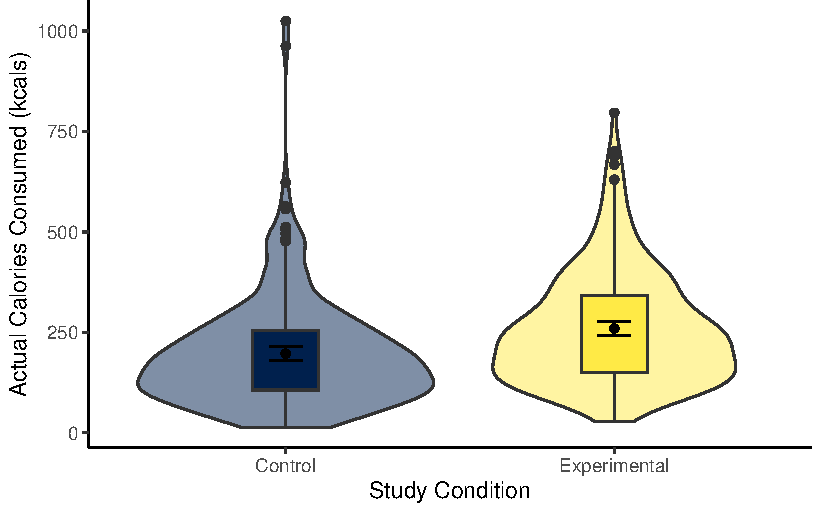
\includegraphics[width=1\textwidth,height=\textheight]{09-lm-categorical_files/figure-pdf/unnamed-chunk-5-1.pdf}
\end{center}

Looking at the graph, the

\begin{itemize}
\tightlist
\item
  \begin{enumerate}
  \def\labelenumi{(\Alph{enumi})}
  \tightlist
  \item
    Control\\
  \end{enumerate}
\item
  \begin{enumerate}
  \def\labelenumi{(\Alph{enumi})}
  \setcounter{enumi}{1}
  \tightlist
  \item
    Experimental
  \end{enumerate}
\end{itemize}

group consumed more calories on average.

\end{tcolorbox}

\begin{tcolorbox}[enhanced jigsaw, breakable, colframe=quarto-callout-caution-color-frame, arc=.35mm, opacitybacktitle=0.6, titlerule=0mm, colbacktitle=quarto-callout-caution-color!10!white, colback=white, toprule=.15mm, bottomtitle=1mm, toptitle=1mm, title=\textcolor{quarto-callout-caution-color}{\faFire}\hspace{0.5em}{Show me the solution}, bottomrule=.15mm, rightrule=.15mm, leftrule=.75mm, coltitle=black, left=2mm, opacityback=0]

The violin-boxplot shows the experimental group who had the biased
visual cues consumed more soup in calories than the control group who
had the accurate visual cues.

You should have the following in a code chunk:

\begin{Shaded}
\begin{Highlighting}[]
\NormalTok{lopez\_clean }\SpecialCharTok{\%\textgreater{}\%} 
  \FunctionTok{ggplot}\NormalTok{(}\FunctionTok{aes}\NormalTok{(}\AttributeTok{y =}\NormalTok{ F\_CaloriesConsumed, }\AttributeTok{x =}\NormalTok{ Condition\_label, }\AttributeTok{fill =}\NormalTok{ Condition\_label)) }\SpecialCharTok{+}
  \FunctionTok{geom\_violin}\NormalTok{(}\AttributeTok{alpha =} \FloatTok{0.5}\NormalTok{) }\SpecialCharTok{+} 
  \FunctionTok{geom\_boxplot}\NormalTok{(}\AttributeTok{width =} \FloatTok{0.2}\NormalTok{, }
               \AttributeTok{fatten =} \ConstantTok{NULL}\NormalTok{) }\SpecialCharTok{+} 
  \FunctionTok{stat\_summary}\NormalTok{(}\AttributeTok{fun =} \StringTok{"mean"}\NormalTok{, }
               \AttributeTok{geom =} \StringTok{"point"}\NormalTok{) }\SpecialCharTok{+}
  \FunctionTok{stat\_summary}\NormalTok{(}\AttributeTok{fun.data =} \StringTok{"mean\_cl\_boot"}\NormalTok{, }\CommentTok{\# confidence interval}
               \AttributeTok{geom =} \StringTok{"errorbar"}\NormalTok{, }
               \AttributeTok{width =} \FloatTok{0.1}\NormalTok{) }\SpecialCharTok{+}
  \FunctionTok{scale\_fill\_viridis\_d}\NormalTok{(}\AttributeTok{option =} \StringTok{"E"}\NormalTok{) }\SpecialCharTok{+} 
  \FunctionTok{scale\_y\_continuous}\NormalTok{(}\AttributeTok{name =} \StringTok{"Actual Calories Consumed (kcals)"}\NormalTok{) }\SpecialCharTok{+}
  \FunctionTok{scale\_x\_discrete}\NormalTok{(}\AttributeTok{name =} \StringTok{"Study Condition"}\NormalTok{) }\SpecialCharTok{+} 
  \FunctionTok{guides}\NormalTok{(}\AttributeTok{fill =} \ConstantTok{FALSE}\NormalTok{) }\SpecialCharTok{+} 
  \FunctionTok{theme\_classic}\NormalTok{()}
\end{Highlighting}
\end{Shaded}

\end{tcolorbox}

\subsection{\texorpdfstring{Activity 4 - Using the \texttt{t.test()}
function}{Activity 4 - Using the t.test() function}}\label{activity-4---using-the-t.test-function}

A t-test is a specific application of the general linear model. In this
test, we express the difference in an outcome between two groups as a
kind of standardised mean difference. If you are interested, see the
Handy Workbook
(\href{https://psyteachr.github.io/handyworkbook/between-subjects-students-t-test.html}{McAleer,
2023}) for the calculations behind the Student and Welch t-test.
Conceptually, a t-test is the difference between two groups divided by
the standard error of the difference. There are two main versions of a
t-test:

\begin{itemize}
\item
  Student t-test
\item
  Welch t-test
\end{itemize}

There is a function built into R to calculate the t-test:
\texttt{t.test()}. The function requires:

\begin{itemize}
\item
  A formula like \texttt{lm()} where you specify the outcome/dependent
  variable and the predictor/independent variable in the form
  \texttt{outcome\ \textasciitilde{}\ predictor}.
\item
  The data set you want to use.
\end{itemize}

For our \texttt{lopez\_clean} data, we would run the following code for
a two-tailed Welch t-test:

\begin{Shaded}
\begin{Highlighting}[]
\FunctionTok{t.test}\NormalTok{(}\AttributeTok{formula =}\NormalTok{ F\_CaloriesConsumed }\SpecialCharTok{\textasciitilde{}}\NormalTok{ Condition\_label, }
       \AttributeTok{data =}\NormalTok{ lopez\_clean)}
\end{Highlighting}
\end{Shaded}

\begin{verbatim}

    Welch Two Sample t-test

data:  F_CaloriesConsumed by Condition_label
t = -4.8578, df = 453.45, p-value = 1.638e-06
alternative hypothesis: true difference in means between group Control and group Experimental is not equal to 0
95 percent confidence interval:
 -88.55610 -37.54289
sample estimates:
     mean in group Control mean in group Experimental 
                  196.6818                   259.7313 
\end{verbatim}

For the three key concepts of inferential statistics, we get

\begin{itemize}
\tightlist
\item
  \textbf{Hypothesis testing}: \emph{p} \textless{} .001, suggesting we
  can reject the null hypothesis assuming \(\alpha\) = .05.
\end{itemize}

\begin{tcolorbox}[enhanced jigsaw, breakable, colframe=quarto-callout-important-color-frame, arc=.35mm, opacitybacktitle=0.6, titlerule=0mm, colbacktitle=quarto-callout-important-color!10!white, colback=white, toprule=.15mm, bottomtitle=1mm, toptitle=1mm, title=\textcolor{quarto-callout-important-color}{\faExclamation}\hspace{0.5em}{What does 1.638e-06 mean?}, bottomrule=.15mm, rightrule=.15mm, leftrule=.75mm, coltitle=black, left=2mm, opacityback=0]

Remember: R reports very small or very large numbers using scientific
notation to save space. We normally report \emph{p}-values to three
decimals, so we report anything smaller as \emph{p} \textless{} .001 to
say it is smaller than this.

If you want to see the real number, you can use the following function
which shows just how small the \emph{p}-value is:

\begin{Shaded}
\begin{Highlighting}[]
\FunctionTok{format}\NormalTok{(}\FloatTok{1.638e{-}06}\NormalTok{, }\AttributeTok{scientific =} \ConstantTok{FALSE}\NormalTok{)}
\end{Highlighting}
\end{Shaded}

\begin{verbatim}
[1] "0.000001638"
\end{verbatim}

\end{tcolorbox}

\begin{itemize}
\tightlist
\item
  \textbf{Effect size}: Somewhat annoyingly, we do not directly get the
  mean difference between groups as a raw/unstandardised mean
  difference. We must manually calculate it by subtracting the means of
  each group (196.6818 - 259.7313 = -63.05). So, those in the
  experimental group ate on average 63 more calories of soup than the
  control group.
\end{itemize}

\begin{tcolorbox}[enhanced jigsaw, breakable, colframe=quarto-callout-important-color-frame, arc=.35mm, opacitybacktitle=0.6, titlerule=0mm, colbacktitle=quarto-callout-important-color!10!white, colback=white, toprule=.15mm, bottomtitle=1mm, toptitle=1mm, title=\textcolor{quarto-callout-important-color}{\faExclamation}\hspace{0.5em}{Does it matter whether the difference is positive or negative?}, bottomrule=.15mm, rightrule=.15mm, leftrule=.75mm, coltitle=black, left=2mm, opacityback=0]

For effect sizes describing the difference between two groups, it is the
absolute difference which is important, providing it is consistent with
your predictions (if applicable). If you entered the groups the other
way around, the mean difference would become 259.7313 - 196.6818 =
63.05. The same applies when we calculate a standardised mean difference
like Cohen's d later.

\end{tcolorbox}

\begin{itemize}
\tightlist
\item
  \textbf{Confidence interval}: {[}-88.56, -37.54{]}, although we do not
  get the mean difference, we get the confidence interval around the
  mean difference.
\end{itemize}

To summarise: A Welch t-test showed participants in the experimental
group ate significantly more calories of soup than participants in the
control group, \emph{t} (453.45) = -4.86, \emph{p} \textless{} .001. On
average, those in the experimental group ate 63.05 (95\% CI = {[}37.54,
88.56{]}) more calories than those in the control group.

When you have statistics software like R to do the heavy lifting for
you, there is not really a scenario where you would use the Student
t-test anymore, but if you did, you can use the \texttt{var.equal}
argument to say you assume there are equal variances in each group:

\begin{Shaded}
\begin{Highlighting}[]
\FunctionTok{t.test}\NormalTok{(}\AttributeTok{formula =}\NormalTok{ F\_CaloriesConsumed }\SpecialCharTok{\textasciitilde{}}\NormalTok{ Condition\_label, }
       \AttributeTok{data =}\NormalTok{ lopez\_clean, }
       \AttributeTok{var.equal =} \ConstantTok{TRUE}\NormalTok{)}
\end{Highlighting}
\end{Shaded}

\begin{verbatim}

    Two Sample t-test

data:  F_CaloriesConsumed by Condition_label
t = -4.8625, df = 462, p-value = 1.591e-06
alternative hypothesis: true difference in means between group Control and group Experimental is not equal to 0
95 percent confidence interval:
 -88.52983 -37.56915
sample estimates:
     mean in group Control mean in group Experimental 
                  196.6818                   259.7313 
\end{verbatim}

You can see the main difference between the two versions is the Welch
t-test Student corrects the degrees of freedom, so they are a decimal.
While the Student t-test does not correct the degrees of freedom, so
they are predictably N - 2.

To summarise: A Student t-test showed participants in the experimental
group ate significantly more calories of soup than participants in the
control group, \emph{t} (462) = -4.86, \emph{p} \textless{} .001. On
average, those in the experimental group ate 63.05 (95\% CI = {[}37.57,
88.53{]}) more calories than those in the control group.

One further useful argument is specifying a one-tailed test if you have
a specific prediction. The only downside to using linear models later is
there is not a simple argument to apply a one-tailed test.

\begin{Shaded}
\begin{Highlighting}[]
\FunctionTok{t.test}\NormalTok{(}\AttributeTok{formula =}\NormalTok{ F\_CaloriesConsumed }\SpecialCharTok{\textasciitilde{}}\NormalTok{ Condition\_label, }
       \AttributeTok{data =}\NormalTok{ lopez\_clean, }
       \AttributeTok{alternative =} \StringTok{"less"}\NormalTok{)}
\end{Highlighting}
\end{Shaded}

\begin{verbatim}

    Welch Two Sample t-test

data:  F_CaloriesConsumed by Condition_label
t = -4.8578, df = 453.45, p-value = 8.188e-07
alternative hypothesis: true difference in means between group Control and group Experimental is less than 0
95 percent confidence interval:
     -Inf -41.6571
sample estimates:
     mean in group Control mean in group Experimental 
                  196.6818                   259.7313 
\end{verbatim}

The difference here is specifying the \texttt{alternative} argument. You
can use ``less'' or ``greater'' depending if you predict a negative
(group A \textless{} group B) or positive difference (group A
\textgreater{} group B).

\subsection{Reporting your t-test
reproducibly}\label{reporting-your-t-test-reproducibly}

Like correlations in Chapter 8, we can take objects like a t-test and
add a little code to format the numbers into APA format. This means you
can report your results reproducibly and avoid potential copy and paste
errors.

For t-tests, the first step is saving your \texttt{t.test()} function as
an object.

\begin{Shaded}
\begin{Highlighting}[]
\NormalTok{lopez\_calories\_object }\OtherTok{\textless{}{-}} \FunctionTok{t.test}\NormalTok{(}\AttributeTok{formula =}\NormalTok{ F\_CaloriesConsumed }\SpecialCharTok{\textasciitilde{}}\NormalTok{ Condition\_label, }
                                \AttributeTok{data =}\NormalTok{ lopez\_clean)}
\end{Highlighting}
\end{Shaded}

If you look in the Environment, you now have an object called
\texttt{lopez\_calories\_object} which is a list of 10 items. For the
following code, this is a function we have created, so we do not expect
you to understand everything at this point as the objects are a little
awkward to work with. You just need to copy and paste it into your .Rmd
file before you want to reference the t-test. Click show the t-test
formatting function as we initially hide it to avoid taking up lots of
space.

\begin{Shaded}
\begin{Highlighting}[]
\NormalTok{report\_ttest }\OtherTok{\textless{}{-}} \ControlFlowTok{function}\NormalTok{(ttest\_object)\{}
  \CommentTok{\# This function will only work for t{-}test objects}
  \CommentTok{\# Step 1 = save all the numbers with formatting }
\NormalTok{  tval }\OtherTok{\textless{}{-}} \FunctionTok{sprintf}\NormalTok{(}\StringTok{"\%.2f"}\NormalTok{, }\FunctionTok{round}\NormalTok{(ttest\_object}\SpecialCharTok{$}\NormalTok{statistic, }\DecValTok{2}\NormalTok{))}
  \CommentTok{\# save degrees of freedom}
\NormalTok{  df }\OtherTok{\textless{}{-}} \FunctionTok{round}\NormalTok{(ttest\_object}\SpecialCharTok{$}\NormalTok{parameter, }\DecValTok{2}\NormalTok{)}
  \CommentTok{\# save p value with formatting if less than .001}
\NormalTok{  pval }\OtherTok{\textless{}{-}}\NormalTok{ ttest\_object}\SpecialCharTok{$}\NormalTok{p.value}
  \ControlFlowTok{if}\NormalTok{ (pval }\SpecialCharTok{\textgreater{}=} \FloatTok{0.001}\NormalTok{)\{}
\NormalTok{    pval }\OtherTok{\textless{}{-}} \FunctionTok{str\_sub}\NormalTok{(}\FunctionTok{as.character}\NormalTok{(pval), }\DecValTok{2}\NormalTok{, }\DecValTok{5}\NormalTok{)}
\NormalTok{    pval }\OtherTok{\textless{}{-}}  \FunctionTok{paste0}\NormalTok{(}\StringTok{", $p$ = "}\NormalTok{, pval)}
  \CommentTok{\# If p \textless{} .001, manually format as p \textless{} .001}
\NormalTok{  \} }\ControlFlowTok{else} \ControlFlowTok{if}\NormalTok{ (pval }\SpecialCharTok{\textless{}} \FloatTok{0.001}\NormalTok{)\{}
\NormalTok{    pval }\OtherTok{\textless{}{-}} \StringTok{", $p$ \textless{} .001"}
\NormalTok{  \}}
  \CommentTok{\# save mean difference}
\NormalTok{  meandiff }\OtherTok{\textless{}{-}} \FunctionTok{round}\NormalTok{(ttest\_object}\SpecialCharTok{$}\NormalTok{estimate[}\DecValTok{1}\NormalTok{] }\SpecialCharTok{{-}}\NormalTok{ ttest\_object}\SpecialCharTok{$}\NormalTok{estimate[}\DecValTok{2}\NormalTok{], }\DecValTok{2}\NormalTok{)}
  \CommentTok{\# save lower 95\% CI}
\NormalTok{  lower\_CI }\OtherTok{\textless{}{-}} \FunctionTok{round}\NormalTok{(ttest\_object}\SpecialCharTok{$}\NormalTok{conf.int[}\DecValTok{1}\NormalTok{], }\DecValTok{2}\NormalTok{)}
  \CommentTok{\# save lower 95\% CI}
\NormalTok{  upper\_CI }\OtherTok{\textless{}{-}} \FunctionTok{round}\NormalTok{(ttest\_object}\SpecialCharTok{$}\NormalTok{conf.int[}\DecValTok{2}\NormalTok{], }\DecValTok{2}\NormalTok{)}
  
  \CommentTok{\# Step 2 = add them together in APA format}
\NormalTok{  output }\OtherTok{\textless{}{-}} \FunctionTok{paste0}\NormalTok{(}\StringTok{"*t* ("}\NormalTok{, df,}\StringTok{") = "}\NormalTok{,}
\NormalTok{                   tval,}
\NormalTok{                   pval,}
                   \StringTok{", mean difference = "}\NormalTok{, meandiff,}
                   \StringTok{", 95\% CI = ["}\NormalTok{, lower\_CI, }\StringTok{", "}\NormalTok{, upper\_CI, }\StringTok{"]"}\NormalTok{)}
  
  \FunctionTok{return}\NormalTok{(output)}
\NormalTok{\}}
\end{Highlighting}
\end{Shaded}

Once you have saved the object and added the formatting function, you
can use the function to format your t-test:

\begin{Shaded}
\begin{Highlighting}[]
\FunctionTok{report\_ttest}\NormalTok{(lopez\_calories\_object)}
\end{Highlighting}
\end{Shaded}

\begin{verbatim}
[1] "*t* (453.45) = -4.86, $p$ < .001, mean difference = -63.05, 95% CI = [-88.56, -37.54]"
\end{verbatim}

You can add that as inline code to insert into your report to make your
inferential statistics reproducible. Just note it's difficult to apply
all the APA format details, so you might need to remove leading zeros,
add italics to the math symbols etc.

\subsection{Activity 5 - Analysing ranks with the Mann-Whitney U
test}\label{activity-5---analysing-ranks-with-the-mann-whitney-u-test}

As a final type of test variation here, like the Spearman is a
non-parametric version of correlation, the Mann-Whitney U test is a
non-parametric version of a t-test. Instead of using the raw values,
this test compares ranks between each group. You can use it when there
are concerns with normality, outliers, or you are analysing a strictly
ordinal outcome (more in Chapter 11).

The format is the same as for the t-test, but instead of the
\texttt{t.test()} function, you have the \texttt{wilcox.test()} function
(it also goes by the name Wilcoxon rank sum test).

\begin{Shaded}
\begin{Highlighting}[]
\FunctionTok{wilcox.test}\NormalTok{(}\AttributeTok{formula =}\NormalTok{ F\_CaloriesConsumed }\SpecialCharTok{\textasciitilde{}}\NormalTok{ Condition\_label, }
            \AttributeTok{data =}\NormalTok{ lopez\_clean,}
            \AttributeTok{conf.int =} \ConstantTok{TRUE}\NormalTok{)}
\end{Highlighting}
\end{Shaded}

\begin{verbatim}

    Wilcoxon rank sum test with continuity correction

data:  F_CaloriesConsumed by Condition_label
W = 18827, p-value = 3.021e-08
alternative hypothesis: true location shift is not equal to 0
95 percent confidence interval:
 -82.06643 -39.92418
sample estimates:
difference in location 
             -59.88637 
\end{verbatim}

The output is similar to the t-test, but adapted to analysing ranks in a
non-parametric test. By setting the argument \texttt{conf.int} to TRUE,
you get the unstandardised effect size and it's confidence interval.
Instead of the mean difference, you get the ``difference in location''.
This represents - to quote the documentation as it is a little awkward -
``the median of the difference between a sample from x and a sample from
y''. This means it is like a difference in medians, but the median
difference in samples from each group rather than the median of the
whole group.

To summarise: A Mann-Whitney U test showed participants in the
experimental group ate significantly more calories of soup than
participants in the control group, \emph{W} = 18827, \emph{p}
\textless{} .001. For the difference in location, those in the
experimental group ate 59.89 (95\% CI = {[}39.92, 82.07{]}) more
calories than those in the control group.

If you wanted to report this reproducibly, you first need to save the
test as an object.

\begin{Shaded}
\begin{Highlighting}[]
\NormalTok{mannwhitney\_cal }\OtherTok{\textless{}{-}} \FunctionTok{wilcox.test}\NormalTok{(}\AttributeTok{formula =}\NormalTok{ F\_CaloriesConsumed }\SpecialCharTok{\textasciitilde{}}\NormalTok{ Condition\_label, }
                               \AttributeTok{data =}\NormalTok{ lopez\_clean,}
                               \AttributeTok{conf.int =} \ConstantTok{TRUE}\NormalTok{)}
\end{Highlighting}
\end{Shaded}

We have then created a bespoke reporting function for the Mann-Whitney U
test.

\begin{Shaded}
\begin{Highlighting}[]
\NormalTok{report\_mannwhitney }\OtherTok{\textless{}{-}} \ControlFlowTok{function}\NormalTok{(mannwhitney\_object)\{}
  \CommentTok{\# This function will only work for Wilcoxon.test objects}
  \CommentTok{\# Step 1 = save all the numbers with formatting }
\NormalTok{  wval }\OtherTok{\textless{}{-}} \FunctionTok{round}\NormalTok{(mannwhitney\_object}\SpecialCharTok{$}\NormalTok{statistic, }\DecValTok{2}\NormalTok{)}
  \CommentTok{\# save p value with formatting if less than .001}
\NormalTok{  pval }\OtherTok{\textless{}{-}}\NormalTok{ mannwhitney\_object}\SpecialCharTok{$}\NormalTok{p.value}
  \ControlFlowTok{if}\NormalTok{ (pval }\SpecialCharTok{\textgreater{}=} \FloatTok{0.001}\NormalTok{)\{}
\NormalTok{    pval }\OtherTok{\textless{}{-}} \FunctionTok{str\_sub}\NormalTok{(}\FunctionTok{as.character}\NormalTok{(pval), }\DecValTok{2}\NormalTok{, }\DecValTok{5}\NormalTok{)}
\NormalTok{    pval }\OtherTok{\textless{}{-}}  \FunctionTok{paste0}\NormalTok{(}\StringTok{", $p$ = "}\NormalTok{, pval)}
  \CommentTok{\# If p \textless{} .001, manually format as p \textless{} .001}
\NormalTok{  \} }\ControlFlowTok{else} \ControlFlowTok{if}\NormalTok{ (pval }\SpecialCharTok{\textless{}} \FloatTok{0.001}\NormalTok{)\{}
\NormalTok{    pval }\OtherTok{\textless{}{-}} \StringTok{", $p$ \textless{} .001"}
\NormalTok{  \}}
  \CommentTok{\# save location difference}
\NormalTok{  locationdiff }\OtherTok{\textless{}{-}} \FunctionTok{round}\NormalTok{(mannwhitney\_object}\SpecialCharTok{$}\NormalTok{estimate, }\DecValTok{2}\NormalTok{)}
  \CommentTok{\# save lower 95\% CI}
\NormalTok{  lower\_CI }\OtherTok{\textless{}{-}} \FunctionTok{round}\NormalTok{(mannwhitney\_object}\SpecialCharTok{$}\NormalTok{conf.int[}\DecValTok{1}\NormalTok{], }\DecValTok{2}\NormalTok{)}
  \CommentTok{\# save lower 95\% CI}
\NormalTok{  upper\_CI }\OtherTok{\textless{}{-}} \FunctionTok{round}\NormalTok{(mannwhitney\_object}\SpecialCharTok{$}\NormalTok{conf.int[}\DecValTok{2}\NormalTok{], }\DecValTok{2}\NormalTok{)}
  
  \CommentTok{\# Step 2 = add them together in APA format}
\NormalTok{  output }\OtherTok{\textless{}{-}} \FunctionTok{paste0}\NormalTok{(}\StringTok{"*W* = "}\NormalTok{, wval,}
\NormalTok{                   pval,}
                   \StringTok{", location difference = "}\NormalTok{, locationdiff,}
                   \StringTok{", 95\% CI = ["}\NormalTok{, lower\_CI, }\StringTok{", "}\NormalTok{, upper\_CI, }\StringTok{"]"}\NormalTok{)}
  
  \FunctionTok{return}\NormalTok{(output)}
\NormalTok{\}}
\end{Highlighting}
\end{Shaded}

Once you have saved the object and added the formatting function, you
can use the function to format your Mann-Whitney U test:

\begin{Shaded}
\begin{Highlighting}[]
\FunctionTok{report\_mannwhitney}\NormalTok{(mannwhitney\_cal)}
\end{Highlighting}
\end{Shaded}

\begin{verbatim}
[1] "*W* = 18827, $p$ < .001, location difference = -59.89, 95% CI = [-82.07, -39.92]"
\end{verbatim}

\subsection{Activity 6 - Calculating Cohen's
d}\label{activity-6---calculating-cohens-d}

Raw/unstandardised effect sizes are great for putting results in
context, particularly when the units are comparable across studies. For
our outcome in this study, differences in calories are easy to put in
context.

Alternatively, it can be useful to calculate standardised effect sizes.
This helps for power analyses (more on that in Chapter 10) and when you
want to compare across comparable studies with slightly different
measurement scales.

There are different formulas for calculating Cohen's d, but if you know
the t-value and degrees of freedom, you can calculate Cohen's d through:

\(d = \frac{2t}{\sqrt{df}} = \frac{-9.725}{21.49} = -0.45\)

It is important to know the concepts before you use shortcuts, but there
is the \texttt{cohens\_d()} function from the effectsize package which
uses the same format as \texttt{t.test()}.

\begin{Shaded}
\begin{Highlighting}[]
\FunctionTok{cohens\_d}\NormalTok{(F\_CaloriesConsumed }\SpecialCharTok{\textasciitilde{}}\NormalTok{ Condition\_label, }
         \AttributeTok{data =}\NormalTok{ lopez\_clean)}
\end{Highlighting}
\end{Shaded}

\begin{verbatim}
Cohen's d |         95% CI
--------------------------
-0.45     | [-0.64, -0.27]

- Estimated using pooled SD.
\end{verbatim}

\begin{tcolorbox}[enhanced jigsaw, breakable, colframe=quarto-callout-tip-color-frame, arc=.35mm, opacitybacktitle=0.6, titlerule=0mm, colbacktitle=quarto-callout-tip-color!10!white, colback=white, toprule=.15mm, bottomtitle=1mm, toptitle=1mm, title=\textcolor{quarto-callout-tip-color}{\faLightbulb}\hspace{0.5em}{Try this}, bottomrule=.15mm, rightrule=.15mm, leftrule=.75mm, coltitle=black, left=2mm, opacityback=0]

Great work following along so far, but now it is time to test your
understanding on a new set of variables. Use the variables
\texttt{CalEstimate} and \texttt{Condition\_label} from
\texttt{lopez\_clean}. We can ask the question: ``What is the difference
in estimated calories consumed between the experimental and control
groups?''

\begin{enumerate}
\def\labelenumi{\arabic{enumi}.}
\item
  Create a violin-boxplot to visualise the difference between
  \texttt{CalEstimate} and \texttt{Condition\_label} from
  \texttt{lopez\_clean}.
\item
  Apply the Welch t-test to get your inferential statistics and answer
  the following questions:

  \begin{itemize}
  \tightlist
  \item
    \textbf{Hypothesis testing}: Assuming \(\alpha\) = .05, the
    difference between the experimental and control groups on estimated
    calories consumed was
  \end{itemize}
\end{enumerate}

\begin{itemize}
\tightlist
\item
  \begin{enumerate}
  \def\labelenumi{(\Alph{enumi})}
  \tightlist
  \item
    statistically significant\\
  \end{enumerate}
\item
  \begin{enumerate}
  \def\labelenumi{(\Alph{enumi})}
  \setcounter{enumi}{1}
  \tightlist
  \item
    not statistically significant
  \end{enumerate}
\end{itemize}

.

\begin{verbatim}
- **Effect size**: Rounded to 2 decimals, the raw effect size was an average difference of _____ estimates calories between the two groups. Expressed as a standardised effect size, this difference equates to Cohen's *d* = ____. 

- **Confidence interval**: Rounded to 2 decimals, the 95% confidence interval for the mean difference is 
\end{verbatim}

\begin{itemize}
\tightlist
\item
  \begin{enumerate}
  \def\labelenumi{(\Alph{enumi})}
  \tightlist
  \item
    -4.08\\
  \end{enumerate}
\item
  \begin{enumerate}
  \def\labelenumi{(\Alph{enumi})}
  \setcounter{enumi}{1}
  \tightlist
  \item
    -0.03\\
  \end{enumerate}
\item
  \begin{enumerate}
  \def\labelenumi{(\Alph{enumi})}
  \setcounter{enumi}{2}
  \tightlist
  \item
    39.85\\
  \end{enumerate}
\item
  \begin{enumerate}
  \def\labelenumi{(\Alph{enumi})}
  \setcounter{enumi}{3}
  \tightlist
  \item
    0.33
  \end{enumerate}
\end{itemize}

to

\begin{itemize}
\tightlist
\item
  \begin{enumerate}
  \def\labelenumi{(\Alph{enumi})}
  \tightlist
  \item
    -4.08\\
  \end{enumerate}
\item
  \begin{enumerate}
  \def\labelenumi{(\Alph{enumi})}
  \setcounter{enumi}{1}
  \tightlist
  \item
    -0.03\\
  \end{enumerate}
\item
  \begin{enumerate}
  \def\labelenumi{(\Alph{enumi})}
  \setcounter{enumi}{2}
  \tightlist
  \item
    39.85\\
  \end{enumerate}
\item
  \begin{enumerate}
  \def\labelenumi{(\Alph{enumi})}
  \setcounter{enumi}{3}
  \tightlist
  \item
    0.33
  \end{enumerate}
\end{itemize}

. The 95\% confidence interval for Cohen's d is

\begin{itemize}
\tightlist
\item
  \begin{enumerate}
  \def\labelenumi{(\Alph{enumi})}
  \tightlist
  \item
    -4.08\\
  \end{enumerate}
\item
  \begin{enumerate}
  \def\labelenumi{(\Alph{enumi})}
  \setcounter{enumi}{1}
  \tightlist
  \item
    -0.03\\
  \end{enumerate}
\item
  \begin{enumerate}
  \def\labelenumi{(\Alph{enumi})}
  \setcounter{enumi}{2}
  \tightlist
  \item
    39.85\\
  \end{enumerate}
\item
  \begin{enumerate}
  \def\labelenumi{(\Alph{enumi})}
  \setcounter{enumi}{3}
  \tightlist
  \item
    0.33
  \end{enumerate}
\end{itemize}

to

\begin{itemize}
\tightlist
\item
  \begin{enumerate}
  \def\labelenumi{(\Alph{enumi})}
  \tightlist
  \item
    -4.08\\
  \end{enumerate}
\item
  \begin{enumerate}
  \def\labelenumi{(\Alph{enumi})}
  \setcounter{enumi}{1}
  \tightlist
  \item
    -0.03\\
  \end{enumerate}
\item
  \begin{enumerate}
  \def\labelenumi{(\Alph{enumi})}
  \setcounter{enumi}{2}
  \tightlist
  \item
    39.85\\
  \end{enumerate}
\item
  \begin{enumerate}
  \def\labelenumi{(\Alph{enumi})}
  \setcounter{enumi}{3}
  \tightlist
  \item
    0.33
  \end{enumerate}
\end{itemize}

.

\end{tcolorbox}

\begin{tcolorbox}[enhanced jigsaw, breakable, colframe=quarto-callout-caution-color-frame, arc=.35mm, opacitybacktitle=0.6, titlerule=0mm, colbacktitle=quarto-callout-caution-color!10!white, colback=white, toprule=.15mm, bottomtitle=1mm, toptitle=1mm, title=\textcolor{quarto-callout-caution-color}{\faFire}\hspace{0.5em}{Show me the solution}, bottomrule=.15mm, rightrule=.15mm, leftrule=.75mm, coltitle=black, left=2mm, opacityback=0]

The violin-boxplot shows little difference between the two groups on
estimated calories consumed.

\begin{Shaded}
\begin{Highlighting}[]
\NormalTok{lopez\_clean }\SpecialCharTok{\%\textgreater{}\%} 
  \FunctionTok{ggplot}\NormalTok{(}\FunctionTok{aes}\NormalTok{(}\AttributeTok{y =}\NormalTok{ CalEstimate, }\AttributeTok{x =}\NormalTok{ Condition\_label, }\AttributeTok{fill =}\NormalTok{ Condition\_label)) }\SpecialCharTok{+}
  \FunctionTok{geom\_violin}\NormalTok{(}\AttributeTok{alpha =} \FloatTok{0.5}\NormalTok{) }\SpecialCharTok{+} 
  \FunctionTok{geom\_boxplot}\NormalTok{(}\AttributeTok{width =} \FloatTok{0.2}\NormalTok{, }
               \AttributeTok{fatten =} \ConstantTok{NULL}\NormalTok{) }\SpecialCharTok{+} 
  \FunctionTok{stat\_summary}\NormalTok{(}\AttributeTok{fun =} \StringTok{"mean"}\NormalTok{, }
               \AttributeTok{geom =} \StringTok{"point"}\NormalTok{) }\SpecialCharTok{+}
  \FunctionTok{stat\_summary}\NormalTok{(}\AttributeTok{fun.data =} \StringTok{"mean\_cl\_boot"}\NormalTok{, }\CommentTok{\# confidence interval}
               \AttributeTok{geom =} \StringTok{"errorbar"}\NormalTok{, }
               \AttributeTok{width =} \FloatTok{0.1}\NormalTok{) }\SpecialCharTok{+}
  \FunctionTok{scale\_fill\_viridis\_d}\NormalTok{(}\AttributeTok{option =} \StringTok{"E"}\NormalTok{) }\SpecialCharTok{+} 
  \FunctionTok{scale\_y\_continuous}\NormalTok{(}\AttributeTok{name =} \StringTok{"Estimated Calories Consumed (kcals)"}\NormalTok{) }\SpecialCharTok{+}
  \FunctionTok{scale\_x\_discrete}\NormalTok{(}\AttributeTok{name =} \StringTok{"Study Condition"}\NormalTok{) }\SpecialCharTok{+} 
  \FunctionTok{guides}\NormalTok{(}\AttributeTok{fill =} \ConstantTok{FALSE}\NormalTok{) }\SpecialCharTok{+} 
  \FunctionTok{theme\_classic}\NormalTok{()}
\end{Highlighting}
\end{Shaded}

\begin{center}
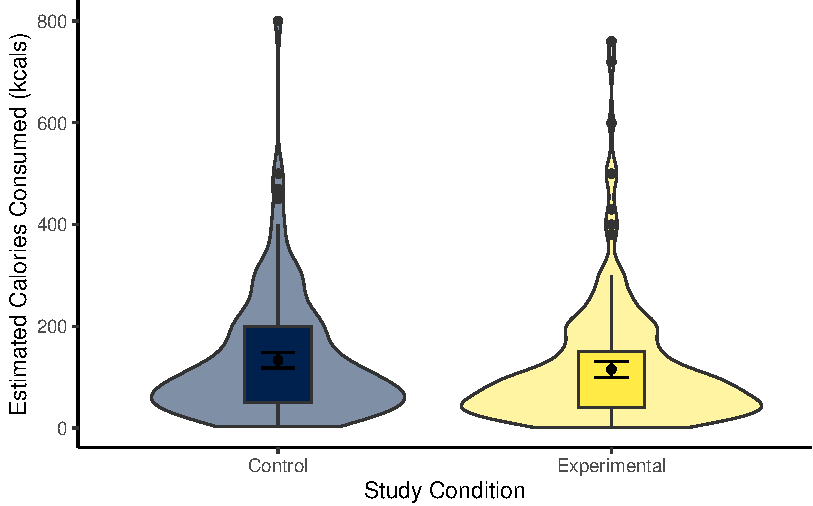
\includegraphics[width=1\textwidth,height=\textheight]{09-lm-categorical_files/figure-pdf/unnamed-chunk-19-1.pdf}
\end{center}

For our inferential statistics, a Welch t-test showed the difference is
not statistically significant, \emph{t} (455.06) = 1.60, \emph{p} =
.110.

\begin{Shaded}
\begin{Highlighting}[]
\FunctionTok{t.test}\NormalTok{(}\AttributeTok{formula =}\NormalTok{ CalEstimate }\SpecialCharTok{\textasciitilde{}}\NormalTok{ Condition\_label, }
       \AttributeTok{data =}\NormalTok{ lopez\_clean)}
\end{Highlighting}
\end{Shaded}

\begin{verbatim}

    Welch Two Sample t-test

data:  CalEstimate by Condition_label
t = 1.6001, df = 455.06, p-value = 0.1103
alternative hypothesis: true difference in means between group Control and group Experimental is not equal to 0
95 percent confidence interval:
 -4.080399 39.846433
sample estimates:
     mean in group Control mean in group Experimental 
                  133.0328                   115.1498 
\end{verbatim}

The control group estimated they consumed 17.88 (95\% CI = {[}-4.08,
39.85{]}) more calories than the experimental group, but the difference
was not significant. Expressed as a standardised effect size, this
equates to Cohen's d = 0.15 (95\% CI = {[}-0.03, 0.33{]}).

\begin{Shaded}
\begin{Highlighting}[]
\FunctionTok{cohens\_d}\NormalTok{(CalEstimate }\SpecialCharTok{\textasciitilde{}}\NormalTok{ Condition\_label, }
         \AttributeTok{data =}\NormalTok{ lopez\_clean)}
\end{Highlighting}
\end{Shaded}

\begin{verbatim}
Cohen's d |        95% CI
-------------------------
0.15      | [-0.03, 0.33]

- Estimated using pooled SD.
\end{verbatim}

\end{tcolorbox}

\section{Linear regression with one categorical
predictor}\label{09-categorical}

Now you know how to calculate a t-test in R, we can turn to simple
linear regression as a more flexible tool for modelling the difference
between two groups. As a reminder, there is a chapter in the Handy
Workbook
(\href{https://psyteachr.github.io/handyworkbook/simple-linear-regression.html}{McAleer,
2023}) dedicated to manually calculating simple linear regression if you
want to work through what the functions are doing behind the scenes.

\subsection{Activity 7 - Descriptive
statistics}\label{activity-7---descriptive-statistics}

For all the information we want to include in a report, calculating
descriptive statistics is helpful for the reader to show the context
behind the results you present. Here, we can report the mean and
standard deviation of our outcome per group.

\begin{Shaded}
\begin{Highlighting}[]
\NormalTok{lopez\_clean }\SpecialCharTok{\%\textgreater{}\%} 
  \FunctionTok{group\_by}\NormalTok{(Condition\_label) }\SpecialCharTok{\%\textgreater{}\%} 
  \FunctionTok{summarise}\NormalTok{(}\AttributeTok{mean\_cals =} \FunctionTok{round}\NormalTok{(}\FunctionTok{mean}\NormalTok{(F\_CaloriesConsumed), }\DecValTok{2}\NormalTok{), }
            \AttributeTok{sd\_cals =} \FunctionTok{round}\NormalTok{(}\FunctionTok{sd}\NormalTok{(F\_CaloriesConsumed), }\DecValTok{2}\NormalTok{))}
\end{Highlighting}
\end{Shaded}

\begin{verbatim}
# A tibble: 2 x 3
  Condition_label mean_cals sd_cals
  <chr>               <dbl>   <dbl>
1 Control              197.    138.
2 Experimental         260.    141.
\end{verbatim}

\begin{tcolorbox}[enhanced jigsaw, breakable, colframe=quarto-callout-note-color-frame, arc=.35mm, opacitybacktitle=0.6, titlerule=0mm, colbacktitle=quarto-callout-note-color!10!white, colback=white, toprule=.15mm, bottomtitle=1mm, toptitle=1mm, title=\textcolor{quarto-callout-note-color}{\faInfo}\hspace{0.5em}{Note}, bottomrule=.15mm, rightrule=.15mm, leftrule=.75mm, coltitle=black, left=2mm, opacityback=0]

If you want some reinforcement of how these skills apply to published
research, look at Table 1 in Lopez et al. (2023). The means and standard
deviations here (and Cohen's d from Activity 5) exactly reproduce the
values they report, apart from the \emph{SD} for the control group
(maybe there is a typo in their article).

\end{tcolorbox}

\subsection{\texorpdfstring{Activity 8 - Using the \texttt{lm()}
function}{Activity 8 - Using the lm() function}}\label{activity-8---using-the-lm-function}

For our research question of ``is there a difference in actual calories
consumed between the control and experimental group?'', we can address
it with simple linear regression. In this study, we can make causal
conclusions as it was an experiment to randomly allocate people into one
of two groups, but you can also use regression to compare two
self-selecting groups when you cannot make a causal conclusion in
isolation. Think carefully about what you can conclude from your design.

Like Chapter 8, we start by defining our regression model with a formula
in the pattern \texttt{outcome\ \textasciitilde{}\ predictor} and
specify the data frame you want to use. We must then use the
\texttt{summary()} function around your model object to get all the
statistics you need.

There are two ways you can use a categorical predictor. First, we can
code groups numerically which people called dummy coding. You code your
first group 0 and you code your second group as 1, which maps on
directly to how the regression model works. Let's look at the output.

\begin{Shaded}
\begin{Highlighting}[]
\CommentTok{\# Condition as a factor containing 0 and 1}
\NormalTok{lm\_cals\_numbers }\OtherTok{\textless{}{-}} \FunctionTok{lm}\NormalTok{(}\AttributeTok{formula =}\NormalTok{ F\_CaloriesConsumed }\SpecialCharTok{\textasciitilde{}}\NormalTok{ Condition, }
                      \AttributeTok{data =}\NormalTok{ lopez\_clean)}

\FunctionTok{summary}\NormalTok{(lm\_cals\_numbers)}
\end{Highlighting}
\end{Shaded}

\begin{verbatim}

Call:
lm(formula = F_CaloriesConsumed ~ Condition, data = lopez_clean)

Residuals:
    Min      1Q  Median      3Q     Max 
-230.90  -99.09  -24.15   62.83  828.04 

Coefficients:
            Estimate Std. Error t value Pr(>|t|)    
(Intercept)  196.682      8.888  22.130  < 2e-16 ***
Condition1    63.049     12.966   4.863 1.59e-06 ***
---
Signif. codes:  0 '***' 0.001 '**' 0.01 '*' 0.05 '.' 0.1 ' ' 1

Residual standard error: 139.4 on 462 degrees of freedom
Multiple R-squared:  0.04869,   Adjusted R-squared:  0.04663 
F-statistic: 23.64 on 1 and 462 DF,  p-value: 1.591e-06
\end{verbatim}

Compared to when we had a continuous predictor in Chapter 8, the output
is identical. We just need to remember what the key numbers represent.
The intercept is the predicted value of your outcome when your predictor
is set to 0. When we have two groups coded as 0 and 1, this means the
intercept is essentially the mean value of group 0 (here, the control
group). We call this the reference group. You can confirm this by
comparing the intercept estimate 196.68 to the mean value of the control
group we calculated in Activity 6.

The slope estimate then represents how we predict the outcome to change
for every 1-unit increase in the predictor. Since we coded the predictor
0 and 1, this just represents the shift from group 1 to group 2. We call
the group we code as 1 the target group. You see the target group
appended to the variable name, which is \texttt{Condition1} here. So,
for a categorical predictor, the slope represents the mean difference
between the reference group (0) and the target group (1): 63.05. In
contrast to the t-test, this is our raw/unstandardised effect size for
the mean difference we do not need to manually calculate.

\begin{tcolorbox}[enhanced jigsaw, breakable, colframe=quarto-callout-note-color-frame, arc=.35mm, opacitybacktitle=0.6, titlerule=0mm, colbacktitle=quarto-callout-note-color!10!white, colback=white, toprule=.15mm, bottomtitle=1mm, toptitle=1mm, title=\textcolor{quarto-callout-note-color}{\faInfo}\hspace{0.5em}{Does it matter if the slope is positive or negative?}, bottomrule=.15mm, rightrule=.15mm, leftrule=.75mm, coltitle=black, left=2mm, opacityback=0]

When you have a categorical predictor, the sign is only important for
interpreting which group is bigger or smaller. The absolute size is
relevant for the effect size where a larger absolute value indicates a
larger effect. Whether the slope is positive or negative depends on the
order of the groups and which has a larger mean. If the reference is
larger than the target, you will get a negative slope. If the target is
larger than the reference, you will get a positive slope.

\end{tcolorbox}

Like the continuous predictor, we get values for \(R^2\) and adjusted
\(R^2\), showing we explain .046 (in other words, 4.6\%) variance in the
outcome through our condition manipulation. We then get the model fit
statistics, but with a single predictor, the \emph{p}-value is
identifical to the slope.

Alternatively, you can use character labels for your categorical
predictor and it will still work. This time, we use
\texttt{Condition\_label}. By default, it will set the order of the
reference and target groups alphabetically, but you can manually specify
the order by setting factor levels.

\begin{Shaded}
\begin{Highlighting}[]
\CommentTok{\# Condition\_label as characters}
\NormalTok{lm\_cals\_labels }\OtherTok{\textless{}{-}} \FunctionTok{lm}\NormalTok{(}\AttributeTok{formula =}\NormalTok{ F\_CaloriesConsumed }\SpecialCharTok{\textasciitilde{}}\NormalTok{ Condition\_label, }
                     \AttributeTok{data =}\NormalTok{ lopez\_clean)}

\FunctionTok{summary}\NormalTok{(lm\_cals\_labels)}
\end{Highlighting}
\end{Shaded}

\begin{verbatim}

Call:
lm(formula = F_CaloriesConsumed ~ Condition_label, data = lopez_clean)

Residuals:
    Min      1Q  Median      3Q     Max 
-230.90  -99.09  -24.15   62.83  828.04 

Coefficients:
                            Estimate Std. Error t value Pr(>|t|)    
(Intercept)                  196.682      8.888  22.130  < 2e-16 ***
Condition_labelExperimental   63.049     12.966   4.863 1.59e-06 ***
---
Signif. codes:  0 '***' 0.001 '**' 0.01 '*' 0.05 '.' 0.1 ' ' 1

Residual standard error: 139.4 on 462 degrees of freedom
Multiple R-squared:  0.04869,   Adjusted R-squared:  0.04663 
F-statistic: 23.64 on 1 and 462 DF,  p-value: 1.591e-06
\end{verbatim}

\begin{tcolorbox}[enhanced jigsaw, breakable, colframe=quarto-callout-note-color-frame, arc=.35mm, opacitybacktitle=0.6, titlerule=0mm, colbacktitle=quarto-callout-note-color!10!white, colback=white, toprule=.15mm, bottomtitle=1mm, toptitle=1mm, title=\textcolor{quarto-callout-note-color}{\faInfo}\hspace{0.5em}{Note}, bottomrule=.15mm, rightrule=.15mm, leftrule=.75mm, coltitle=black, left=2mm, opacityback=0]

If you want to test specifying the factor order to see how it affects
the output, try running this code prior to the regression model:

\begin{Shaded}
\begin{Highlighting}[]
\CommentTok{\# Specify group order of Experimental then Control}
\NormalTok{lopez\_clean }\OtherTok{\textless{}{-}}\NormalTok{ lopez\_clean }\SpecialCharTok{\%\textgreater{}\%} 
  \FunctionTok{mutate}\NormalTok{(}\AttributeTok{Condition\_label =} \FunctionTok{factor}\NormalTok{(Condition\_label, }
                                  \AttributeTok{levels =} \FunctionTok{c}\NormalTok{(}\StringTok{"Experimental"}\NormalTok{, }\StringTok{"Control"}\NormalTok{)))}
\end{Highlighting}
\end{Shaded}

\end{tcolorbox}

\begin{tcolorbox}[enhanced jigsaw, breakable, colframe=quarto-callout-note-color-frame, arc=.35mm, opacitybacktitle=0.6, titlerule=0mm, colbacktitle=quarto-callout-note-color!10!white, colback=white, toprule=.15mm, bottomtitle=1mm, toptitle=1mm, title=\textcolor{quarto-callout-note-color}{\faInfo}\hspace{0.5em}{How are t-tests and regression the same?}, bottomrule=.15mm, rightrule=.15mm, leftrule=.75mm, coltitle=black, left=2mm, opacityback=0]

If you are interested in the relationship between the two concepts, we
said a t-test was a specific application of the general linear model. In
the t-test calculations, it expresses the mean difference between groups
by the standard error of the difference. In essence, it describes the
difference in standard errors, which we can describe with a
t-distribution to calculate \emph{p}-values.

In regression, we frame the model as how much variance you explain
compared to the total amount of variance. The more variance your
predictor explains, the less unexplained variance there is left over.
For the slope estimate though, this is identical to the t-test as we
estimate the mean difference between groups plus the standard error
around the mean difference. We calculate a \emph{p}-value for the slope
from a t-distribution, so you get a t-value in the output.

You can see the process is identical by comparing the key values from
the regression output to the Student t-test. We can recreate the mean
difference to compare to the slope, the t-value is the same, the p-value
is the same, the degrees of freedom are the same, and the 95\%
confidence intervals below are the same.

So, when you have a single categorical predictor, it is the exact same
process as the Student t-test, just expressed slightly different. The
only downside to this procedure is it is much more difficult to recreate
the Welch t-test.

\end{tcolorbox}

\subsection{Activity 9 - Calculating confidence
intervals}\label{activity-9---calculating-confidence-intervals}

The only thing we are missing is our confidence intervals around the
estimates which we can calculate through the \texttt{confint()}
function.

\begin{Shaded}
\begin{Highlighting}[]
\FunctionTok{confint}\NormalTok{(lm\_cals\_numbers)}
\end{Highlighting}
\end{Shaded}

\begin{verbatim}
                2.5 %    97.5 %
(Intercept) 179.21657 214.14704
Condition1   37.56915  88.52983
\end{verbatim}

Now, we can summarise the three key concepts of inferential statistics
as:

\begin{itemize}
\item
  \textbf{Hypothesis testing}: \emph{p} \textless{} .001, suggesting we
  can reject the null hypothesis assuming \(\alpha\) = .05. The
  experimental group ate significantly more calories of soup than the
  control group.
\item
  \textbf{Effect size}: \(b_1\) = 63.05, suggesting the experimental
  group ate on average 63 more calories than the control group.
\item
  \textbf{Confidence interval}: {[}37.57, 88.53{]}, showing the
  precision around the slope estimate.
\end{itemize}

\begin{tcolorbox}[enhanced jigsaw, breakable, colframe=quarto-callout-tip-color-frame, arc=.35mm, opacitybacktitle=0.6, titlerule=0mm, colbacktitle=quarto-callout-tip-color!10!white, colback=white, toprule=.15mm, bottomtitle=1mm, toptitle=1mm, title=\textcolor{quarto-callout-tip-color}{\faLightbulb}\hspace{0.5em}{Try this}, bottomrule=.15mm, rightrule=.15mm, leftrule=.75mm, coltitle=black, left=2mm, opacityback=0]

Now it is time to test your understanding on a new set of variables.
This time, use \texttt{CalEstimate} as your outcome,
\texttt{Condition\_label} as your predictor, and use
\texttt{lopez\_clean} as your data. We can ask the same question as
Activity 5: ``What is the difference in estimated calories consumed
between the experimental and control groups?''.

Apply simple linear regression to get your inferential statistics and
answer the following questions:

\begin{itemize}
\item
  \textbf{Hypothesis testing}: Assuming \(\alpha\) = .05, Condition is a
\item
  \begin{enumerate}
  \def\labelenumi{(\Alph{enumi})}
  \tightlist
  \item
    statistically significant\\
  \end{enumerate}
\item
  \begin{enumerate}
  \def\labelenumi{(\Alph{enumi})}
  \setcounter{enumi}{1}
  \tightlist
  \item
    non-significant
  \end{enumerate}
\end{itemize}

predictor of estimates calories consumed.

\begin{itemize}
\item
  \textbf{Effect size}: Rounded to 2 decimals, the Condition slope
  coefficient means there was a mean difference of
\item
  \begin{enumerate}
  \def\labelenumi{(\Alph{enumi})}
  \tightlist
  \item
    133.03\\
  \end{enumerate}
\item
  \begin{enumerate}
  \def\labelenumi{(\Alph{enumi})}
  \setcounter{enumi}{1}
  \tightlist
  \item
    7.68\\
  \end{enumerate}
\item
  \begin{enumerate}
  \def\labelenumi{(\Alph{enumi})}
  \setcounter{enumi}{2}
  \tightlist
  \item
    -17.88\\
  \end{enumerate}
\item
  \begin{enumerate}
  \def\labelenumi{(\Alph{enumi})}
  \setcounter{enumi}{3}
  \tightlist
  \item
    11.19
  \end{enumerate}
\end{itemize}

.

\begin{itemize}
\item
  \textbf{Confidence interval}: Rounded to 2 decimals, the lower bound
  of the slope is
\item
  \begin{enumerate}
  \def\labelenumi{(\Alph{enumi})}
  \tightlist
  \item
    117.94\\
  \end{enumerate}
\item
  \begin{enumerate}
  \def\labelenumi{(\Alph{enumi})}
  \setcounter{enumi}{1}
  \tightlist
  \item
    -39.88\\
  \end{enumerate}
\item
  \begin{enumerate}
  \def\labelenumi{(\Alph{enumi})}
  \setcounter{enumi}{2}
  \tightlist
  \item
    148.12\\
  \end{enumerate}
\item
  \begin{enumerate}
  \def\labelenumi{(\Alph{enumi})}
  \setcounter{enumi}{3}
  \tightlist
  \item
    4.11
  \end{enumerate}
\end{itemize}

and the upper bound is

\begin{itemize}
\tightlist
\item
  \begin{enumerate}
  \def\labelenumi{(\Alph{enumi})}
  \tightlist
  \item
    117.94\\
  \end{enumerate}
\item
  \begin{enumerate}
  \def\labelenumi{(\Alph{enumi})}
  \setcounter{enumi}{1}
  \tightlist
  \item
    -39.88\\
  \end{enumerate}
\item
  \begin{enumerate}
  \def\labelenumi{(\Alph{enumi})}
  \setcounter{enumi}{2}
  \tightlist
  \item
    148.12\\
  \end{enumerate}
\item
  \begin{enumerate}
  \def\labelenumi{(\Alph{enumi})}
  \setcounter{enumi}{3}
  \tightlist
  \item
    4.11
  \end{enumerate}
\end{itemize}

.

\end{tcolorbox}

\begin{tcolorbox}[enhanced jigsaw, breakable, colframe=quarto-callout-caution-color-frame, arc=.35mm, opacitybacktitle=0.6, titlerule=0mm, colbacktitle=quarto-callout-caution-color!10!white, colback=white, toprule=.15mm, bottomtitle=1mm, toptitle=1mm, title=\textcolor{quarto-callout-caution-color}{\faFire}\hspace{0.5em}{Show me the solution}, bottomrule=.15mm, rightrule=.15mm, leftrule=.75mm, coltitle=black, left=2mm, opacityback=0]

The conclusions are the same as when we calculated the t-test, where
condition is not a statistically significant predictor of estimated
calories consumed. As a regression model, we get the same conclusions
expressed in a slightly different way. Condition is a negative but
non-significant predictor (\emph{p} = .111). The control group ate 17.88
(\(b_1\) = -17.88, 95\% CI = {[}-39.88, 4.11{]}) more calories than the
experimental group. We explain very little variance in estimated
calories consumed (adjusted \(R^2\) = .003), so the condition
manipulation had little effect.

\begin{Shaded}
\begin{Highlighting}[]
\CommentTok{\# Create lm object for condiiton label as a predictor}
\NormalTok{lm\_cal\_est }\OtherTok{\textless{}{-}} \FunctionTok{lm}\NormalTok{(CalEstimate }\SpecialCharTok{\textasciitilde{}}\NormalTok{ Condition\_label, }
                 \AttributeTok{data =}\NormalTok{ lopez\_clean)}

\CommentTok{\# summary of the model object}
\FunctionTok{summary}\NormalTok{(lm\_cal\_est)}

\CommentTok{\# confidence intervals around estimates}
\FunctionTok{confint}\NormalTok{(lm\_cal\_est)}
\end{Highlighting}
\end{Shaded}

\begin{verbatim}

Call:
lm(formula = CalEstimate ~ Condition_label, data = lopez_clean)

Residuals:
    Min      1Q  Median      3Q     Max 
-130.03  -83.03  -33.03   44.85  666.97 

Coefficients:
                            Estimate Std. Error t value Pr(>|t|)    
(Intercept)                  133.033      7.679  17.324   <2e-16 ***
Condition_labelExperimental  -17.883     11.192  -1.598    0.111    
---
Signif. codes:  0 '***' 0.001 '**' 0.01 '*' 0.05 '.' 0.1 ' ' 1

Residual standard error: 119.9 on 459 degrees of freedom
  (3 observations deleted due to missingness)
Multiple R-squared:  0.005531,  Adjusted R-squared:  0.003365 
F-statistic: 2.553 on 1 and 459 DF,  p-value: 0.1108

                                2.5 %     97.5 %
(Intercept)                 117.94256 148.123015
Condition_labelExperimental -39.87763   4.111599
\end{verbatim}

\end{tcolorbox}

\subsection{Activity 10 - Standardising
predictors}\label{activity-10---standardising-predictors}

For simple linear regression with two levels of a categorical predictor,
centering the variable does not help, but we can standardise our outcome
to express the estimate in standard deviations rather than the raw
units. This is analogous to calculating Cohen's d as we express the
standardised mean difference. In contrast to continuous predictors, we
only need to standardise the outcome, rather than both the outcome and
predictor(s). We then use the standardised variable as our outcome.

\begin{Shaded}
\begin{Highlighting}[]
\CommentTok{\# Be careful with the bracket placement to subtract the mean first}
\NormalTok{lopez\_clean }\OtherTok{\textless{}{-}}\NormalTok{lopez\_clean }\SpecialCharTok{\%\textgreater{}\%} 
  \FunctionTok{mutate}\NormalTok{(}\AttributeTok{actual\_calories\_std =}\NormalTok{ (F\_CaloriesConsumed }\SpecialCharTok{{-}} \FunctionTok{mean}\NormalTok{(F\_CaloriesConsumed)) }\SpecialCharTok{/} \FunctionTok{sd}\NormalTok{(F\_CaloriesConsumed))}

\CommentTok{\# Condition as a factor containing 0 and 1}
\NormalTok{lm\_cals\_std }\OtherTok{\textless{}{-}} \FunctionTok{lm}\NormalTok{(}\AttributeTok{formula =}\NormalTok{ actual\_calories\_std }\SpecialCharTok{\textasciitilde{}}\NormalTok{ Condition, }
                      \AttributeTok{data =}\NormalTok{ lopez\_clean)}

\FunctionTok{summary}\NormalTok{(lm\_cals\_std)}
\end{Highlighting}
\end{Shaded}

\begin{verbatim}

Call:
lm(formula = actual_calories_std ~ Condition, data = lopez_clean)

Residuals:
    Min      1Q  Median      3Q     Max 
-1.6173 -0.6941 -0.1692  0.4401  5.8000 

Coefficients:
            Estimate Std. Error t value Pr(>|t|)    
(Intercept) -0.20749    0.06225  -3.333 0.000928 ***
Condition1   0.44163    0.09082   4.863 1.59e-06 ***
---
Signif. codes:  0 '***' 0.001 '**' 0.01 '*' 0.05 '.' 0.1 ' ' 1

Residual standard error: 0.9764 on 462 degrees of freedom
Multiple R-squared:  0.04869,   Adjusted R-squared:  0.04663 
F-statistic: 23.64 on 1 and 462 DF,  p-value: 1.591e-06
\end{verbatim}

Note, the estimate may be slightly different to directly calculating
Cohen's d as there are a few formulas. If you compare to Activity 5, we
got \emph{d} = 0.45 there and 0.44 here. Between the estimate and 95\%
confidence intervals, they are off by .02, so it does not have a
material impact on the results.

\begin{tcolorbox}[enhanced jigsaw, breakable, colframe=quarto-callout-tip-color-frame, arc=.35mm, opacitybacktitle=0.6, titlerule=0mm, colbacktitle=quarto-callout-tip-color!10!white, colback=white, toprule=.15mm, bottomtitle=1mm, toptitle=1mm, title=\textcolor{quarto-callout-tip-color}{\faLightbulb}\hspace{0.5em}{Tip}, bottomrule=.15mm, rightrule=.15mm, leftrule=.75mm, coltitle=black, left=2mm, opacityback=0]

As before, once you know how it works conceptually, there is a shortcut
where you do not need to standardise all your variables first. The
effectsize package has a handy function called
\texttt{standardize\_parameters()} which you can apply to your initial
\texttt{lm()} object.

\begin{Shaded}
\begin{Highlighting}[]
\FunctionTok{standardize\_parameters}\NormalTok{(lm\_cals\_numbers)}
\end{Highlighting}
\end{Shaded}

\begin{verbatim}
# Standardization method: refit

Parameter     | Std. Coef. |         95% CI
-------------------------------------------
(Intercept)   |      -0.21 | [-0.33, -0.09]
Condition [1] |       0.44 | [ 0.26,  0.62]
\end{verbatim}

\end{tcolorbox}

\section{Checking assumptions}\label{checking-assumptions-1}

For the inferential statistics to work as intended, the model makes
certain assumptions about the data you are putting into it and the
accuracy of the inferences depends on how sensible these assumption are.

\subsection{Activity 11 - Diagnostic plots for linear
regression}\label{activity-11---diagnostic-plots-for-linear-regression}

We have the same assumptions for simple linear regression now we have a
categorical predictor:

\begin{enumerate}
\def\labelenumi{\arabic{enumi}.}
\item
  The outcome is interval/ratio level data.
\item
  The predictor variable is interval/ratio or categorical (with two
  levels at a time).
\item
  All values of the outcome variable are independent (i.e., each score
  should come from a different participant/observation).
\item
  The predictors have non-zero variance.
\item
  The relationship between the outcome and predictor is linear.
\item
  The residuals should be normally distributed.
\item
  There should be homoscedasticity.
\end{enumerate}

Assumptions 1-4 are pretty straight forward as they relate to your
understanding of the design or a simple check on the data for non-zero
variance (the responses are not all the exact same value).

Assumptions 5-7 require diagnostic checks on the residuals from the
model. In contrast to continuous predictors, they are a little harder to
identify patterns in. As we only have two values on the x-axis (0 and
1), all the residuals will be organised into vertical lines and the
trend lines to help spot patterns do not look quite right.

\subsection{Checking linearity}\label{checking-linearity-1}

When you have a categorical predictor with two levels, you meet
linearity by default, so you \textbf{do not} need to check this
assumption directly. When you have two levels, you can only fit a
straight line between the values.

\begin{Shaded}
\begin{Highlighting}[]
\FunctionTok{plot}\NormalTok{(lm\_cals\_numbers, }
     \AttributeTok{which =} \DecValTok{1}\NormalTok{)}
\end{Highlighting}
\end{Shaded}

\begin{center}
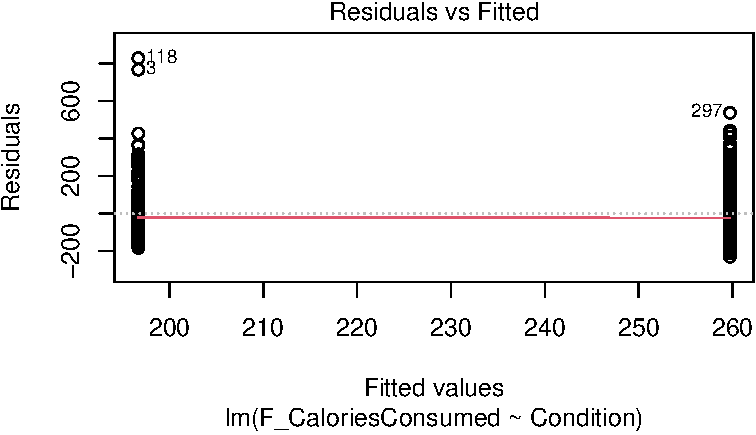
\includegraphics[width=1\textwidth,height=\textheight]{09-lm-categorical_files/figure-pdf/unnamed-chunk-30-1.pdf}
\end{center}

\subsection{Checking normality}\label{checking-normality-1}

The qq-plot is still the same to interpret. Now, this example presents a
useful case of decision making in data analysis we explore more in
Chapter 11. The plot here is approaching signs of violating normality as
there is a clear curve to the data points with 3 and 118 the largest
deviations (you can see these on the violin-boxplot as the two highest
values in the control group). For this chapter, we are sticking with it
and it would be consistent with how the original authors analysed the
data, but note this would be a key decision to make and justify when
reporting the analysis.

\begin{Shaded}
\begin{Highlighting}[]
\FunctionTok{plot}\NormalTok{(lm\_cals\_numbers, }
     \AttributeTok{which =} \DecValTok{2}\NormalTok{)}
\end{Highlighting}
\end{Shaded}

\begin{center}
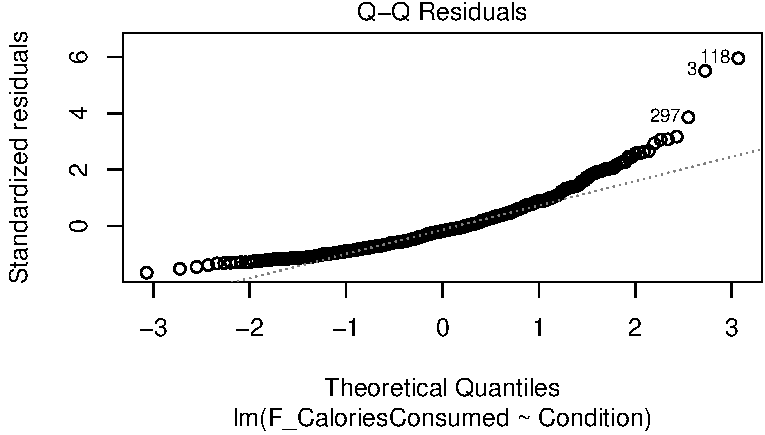
\includegraphics[width=1\textwidth,height=\textheight]{09-lm-categorical_files/figure-pdf/unnamed-chunk-31-1.pdf}
\end{center}

\subsection{Checking
homoscedasticity}\label{checking-homoscedasticity-1}

The scale-location plot is harder to interpret when you have a
categorical predictor. Like linearity, the points are all arranged in
two vertical lines as we only have two levels. You are looking out for
the spread of the two lines to be roughly similar. They look fine here,
just points 118 and 3 separated a little from the other points.

\begin{Shaded}
\begin{Highlighting}[]
\FunctionTok{plot}\NormalTok{(lm\_cals\_numbers, }
     \AttributeTok{which =} \DecValTok{3}\NormalTok{)}
\end{Highlighting}
\end{Shaded}

\begin{center}
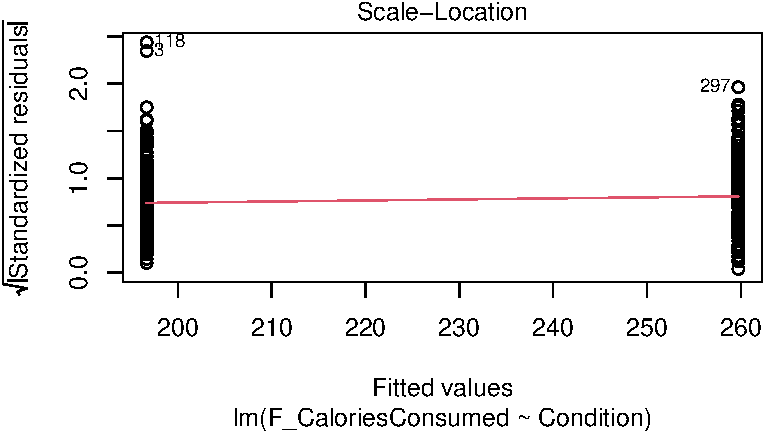
\includegraphics[width=1\textwidth,height=\textheight]{09-lm-categorical_files/figure-pdf/unnamed-chunk-32-1.pdf}
\end{center}

\subsection{Checking influential
cases}\label{checking-influential-cases-1}

Finally, we have our plots for identifying influential cases. First, we
get Cook's distance for all the observations in your data. We see points
3 and 118 come up yet again, but although they are the largest
deviations, they do not necessarily have worrying Cook's distance
values. There are different thresholds in the literature, but estimates
range from 1, 0.5, to 4/n.~It would only be under this final most
conservative estimate (0.009) we would highlight several observations
for further inspection.

\begin{Shaded}
\begin{Highlighting}[]
\FunctionTok{plot}\NormalTok{(lm\_cals\_numbers, }
     \AttributeTok{which =} \DecValTok{4}\NormalTok{)}
\end{Highlighting}
\end{Shaded}

\begin{center}
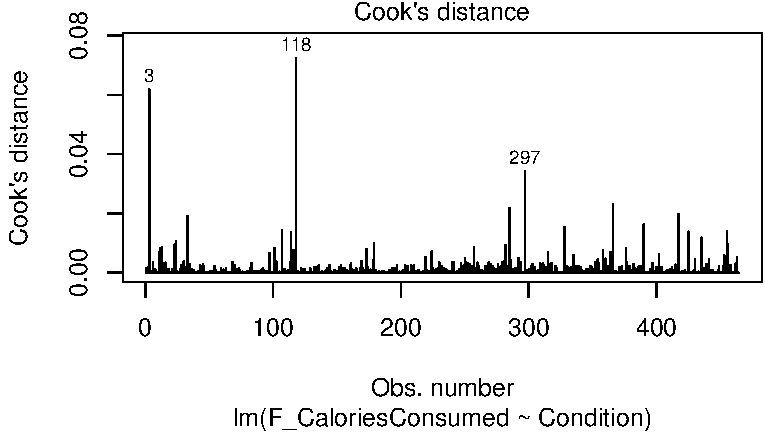
\includegraphics[width=1\textwidth,height=\textheight]{09-lm-categorical_files/figure-pdf/unnamed-chunk-33-1.pdf}
\end{center}

Finally, the fifth plot shows residual values against leverage. Like
Chapter 8, we cannot see the Cook's distance threshold it uses in the
plot as none of the points are a large enough deviation, despite 3 and
188 sticking out again.

\begin{Shaded}
\begin{Highlighting}[]
\FunctionTok{plot}\NormalTok{(lm\_cals\_numbers, }
     \AttributeTok{which =} \DecValTok{5}\NormalTok{)}
\end{Highlighting}
\end{Shaded}

\begin{center}
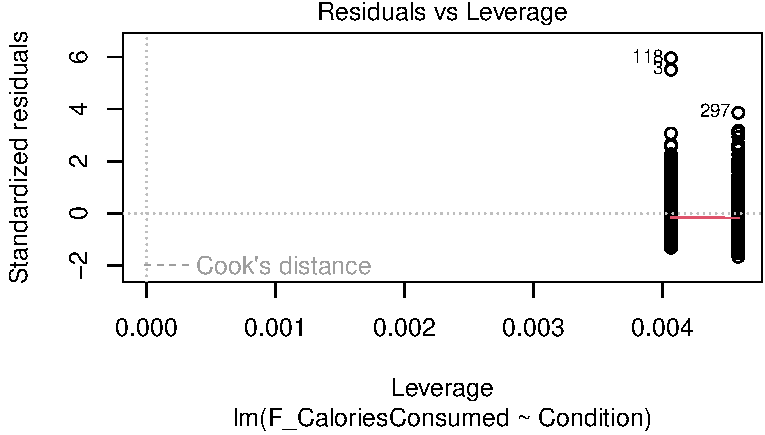
\includegraphics[width=1\textwidth,height=\textheight]{09-lm-categorical_files/figure-pdf/unnamed-chunk-34-1.pdf}
\end{center}

\subsection{Checking all the
assumptions}\label{checking-all-the-assumptions-1}

Now we have covered the individual diagnostic plots, there is a handy
function called \texttt{check\_model()} from the performance package.
Like the \texttt{plot()} function, the output for linearity,
homoscedasticity, and influential observations does not plot right as we
only have two values for the predictor and the plot lines do not really
work. Do not worry, you have not done anything wrong.

\begin{Shaded}
\begin{Highlighting}[]
\FunctionTok{check\_model}\NormalTok{(lm\_cals\_numbers)}
\end{Highlighting}
\end{Shaded}

\begin{center}
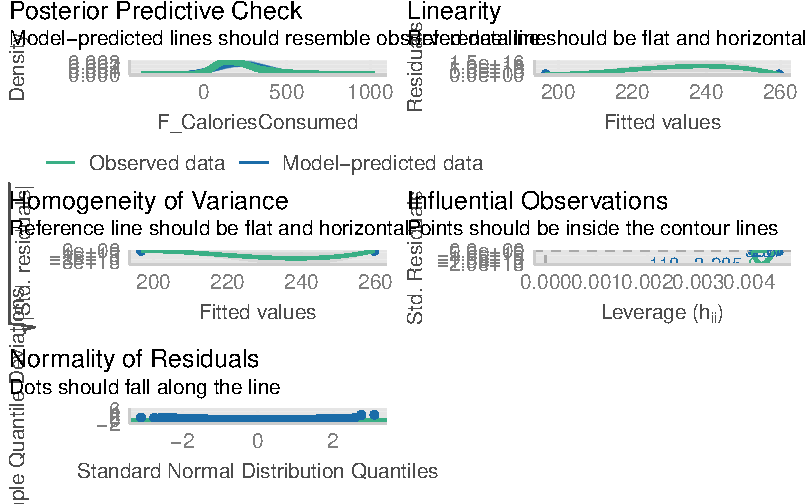
\includegraphics[width=1\textwidth,height=\textheight]{09-lm-categorical_files/figure-pdf/unnamed-chunk-35-1.pdf}
\end{center}

\begin{tcolorbox}[enhanced jigsaw, breakable, colframe=quarto-callout-note-color-frame, arc=.35mm, opacitybacktitle=0.6, titlerule=0mm, colbacktitle=quarto-callout-note-color!10!white, colback=white, toprule=.15mm, bottomtitle=1mm, toptitle=1mm, title=\textcolor{quarto-callout-note-color}{\faInfo}\hspace{0.5em}{What might explain the funky normality?}, bottomrule=.15mm, rightrule=.15mm, leftrule=.75mm, coltitle=black, left=2mm, opacityback=0]

If you are interested, the posterior predictive check here provides an
insight into why we get potential problems with normality. The outcome
is ratio but cannot be smaller than 0 as we cannot have negative
calories. So, in the green line for the observed data, the data are a
little skewed as it drops off prior to 0. However, the model does not
know that and it happily predicts normally distributed values which go
below 0, creating a mismatch between what the model predicts and the
values we enter into it.

Remember the models will work regardless of the data you put into them,
it is important to keep your role in mind to recognise when you need to
be cautious about what you can learn from the model.

\end{tcolorbox}

\begin{tcolorbox}[enhanced jigsaw, breakable, colframe=quarto-callout-tip-color-frame, arc=.35mm, opacitybacktitle=0.6, titlerule=0mm, colbacktitle=quarto-callout-tip-color!10!white, colback=white, toprule=.15mm, bottomtitle=1mm, toptitle=1mm, title=\textcolor{quarto-callout-tip-color}{\faLightbulb}\hspace{0.5em}{Try this}, bottomrule=.15mm, rightrule=.15mm, leftrule=.75mm, coltitle=black, left=2mm, opacityback=0]

In activity 8, you should have calculated the effect of condition
(\texttt{Condition\_label}) on estimated calories consumed
(\texttt{CalEstimate}) for your independent task. Using the model object
\texttt{lm\_cal\_est}, work through assumptions for simple linear
regression and make a note of whether you think it meets the
assumptions, or there might be any problems. Some of the assumptions you
consider what you know about the design, while others you need the
diagnostic plots.

\begin{enumerate}
\def\labelenumi{\arabic{enumi}.}
\item
  The outcome is interval/ratio level data.
\item
  The predictor variable is interval/ratio or categorical (with two
  levels at a time).
\item
  All values of the outcome variable are independent (i.e., each score
  should come from a different participant/observation).
\item
  The predictors have non-zero variance.
\item
  The relationship between the outcome and predictor is linear.
\item
  The residuals should be normally distributed.
\item
  There should be homoscedasticity.
\end{enumerate}

\end{tcolorbox}

\begin{tcolorbox}[enhanced jigsaw, breakable, colframe=quarto-callout-caution-color-frame, arc=.35mm, opacitybacktitle=0.6, titlerule=0mm, colbacktitle=quarto-callout-caution-color!10!white, colback=white, toprule=.15mm, bottomtitle=1mm, toptitle=1mm, title=\textcolor{quarto-callout-caution-color}{\faFire}\hspace{0.5em}{Show me the solution}, bottomrule=.15mm, rightrule=.15mm, leftrule=.75mm, coltitle=black, left=2mm, opacityback=0]

\begin{enumerate}
\def\labelenumi{\arabic{enumi}.}
\tightlist
\item
  The outcome is interval/ratio level data.
\end{enumerate}

\textbf{The outcome is nicely ratio as estimated calories have a logical
0 point (no calories) and the units are in equal measurements..}

\begin{enumerate}
\def\labelenumi{\arabic{enumi}.}
\setcounter{enumi}{1}
\tightlist
\item
  The predictor variable is interval/ratio or categorical (with two
  levels at a time).
\end{enumerate}

\textbf{Our predictor is categorical with two levels.}

\begin{enumerate}
\def\labelenumi{\arabic{enumi}.}
\setcounter{enumi}{2}
\tightlist
\item
  All values of the outcome variable are independent (i.e., each score
  should come from a different participant/observation).
\end{enumerate}

\textbf{The short answer is this appears to be the case in this study.
The longer answer is there might have been an issue with the
participants apparently completing the study in groups of 3. It is not
entirely clear in the data how they recorded this, but grouped data
collection does present a potential problem with independence we do not
tackle in this course and the original authors did not seem to address
it.}

\begin{enumerate}
\def\labelenumi{\arabic{enumi}.}
\setcounter{enumi}{3}
\tightlist
\item
  The predictors have non-zero variance.
\end{enumerate}

\textbf{We have observations from both levels of the predictor.}

\begin{enumerate}
\def\labelenumi{\arabic{enumi}.}
\setcounter{enumi}{4}
\tightlist
\item
  The relationship between the outcome and predictor is linear.
\end{enumerate}

\textbf{We meet linearity by default with two levels, so we do not need
the plot here.}

\begin{enumerate}
\def\labelenumi{\arabic{enumi}.}
\setcounter{enumi}{5}
\tightlist
\item
  The residuals should be normally distributed.
\end{enumerate}

\textbf{Like the actual calories consumed, this is firmly a clear
deviation from what we expect and provides a good example of when it
does not look right. If we were to analyse the data fully, we would
explore the impact of this and alternative models, but for this chapter,
we are going to note our concern and remember the authors analysed the
data like this.}

\begin{Shaded}
\begin{Highlighting}[]
\FunctionTok{plot}\NormalTok{(lm\_cal\_est, }
     \AttributeTok{which =} \DecValTok{2}\NormalTok{)}
\end{Highlighting}
\end{Shaded}

\begin{center}
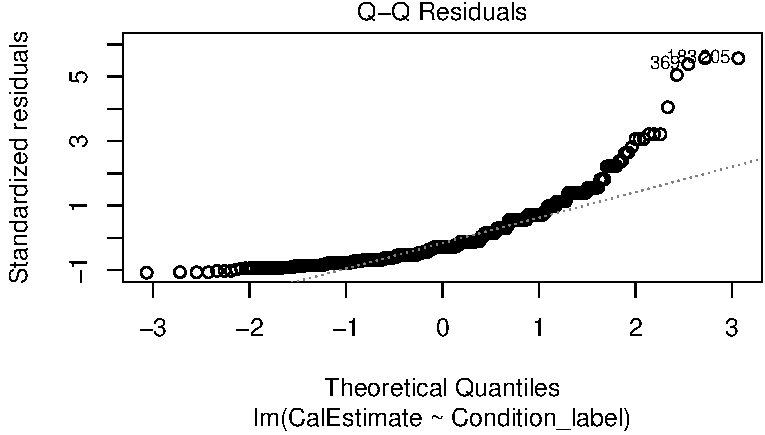
\includegraphics[width=1\textwidth,height=\textheight]{09-lm-categorical_files/figure-pdf/unnamed-chunk-36-1.pdf}
\end{center}

\begin{enumerate}
\def\labelenumi{\arabic{enumi}.}
\setcounter{enumi}{6}
\tightlist
\item
  There should be homoscedasticity.
\end{enumerate}

\textbf{Looking at the spread of each group, it looks fine with a
similar range until both groups are more sparsely distributed above 1.}

\begin{Shaded}
\begin{Highlighting}[]
\FunctionTok{plot}\NormalTok{(lm\_cal\_est, }
     \AttributeTok{which =} \DecValTok{3}\NormalTok{)}
\end{Highlighting}
\end{Shaded}

\begin{center}
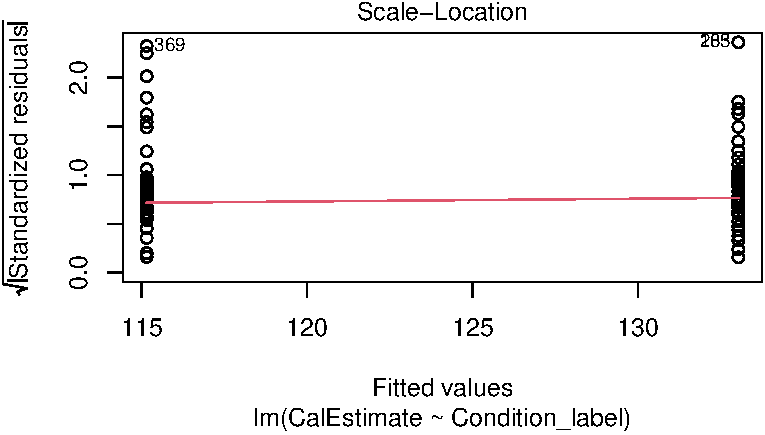
\includegraphics[width=1\textwidth,height=\textheight]{09-lm-categorical_files/figure-pdf/unnamed-chunk-37-1.pdf}
\end{center}

In summary, normality is a clear concern and something we will return to
for your options in Chapter 11 and the course materials. For now, we
will stick with the model but recognise we should be cautious.

\end{tcolorbox}

\section{Reporting your results}\label{reporting-your-results-1}

Now we have some results to go with, there are a few recommendations on
how to communicate that information. If you need a reminder of APA style
for formatting numbers, you can see
\href{https://apastyle.apa.org/instructional-aids/numbers-statistics-guide.pdf}{this
PDF online} for a little cheat sheet for numbers and statistics.

\begin{enumerate}
\def\labelenumi{\arabic{enumi}.}
\item
  Explain to the reader what your linear regression model was. For
  example, what was your outcome and predictor variable?
\item
  Report descriptive statistics to help contextualise your findings. For
  example, the mean/standard deviation for your outcome per group.
\item
  Provide an appropriate data visualisation to help communciate key
  patterns to the reader. For example, a violin-boxplot for how each
  group responded on your outcome.
\item
  Report all three key inferential statistics concepts for the
  coefficient: the slope, the confidence interval around your slope, and
  the \emph{p}-value for hypothesis testing. When you have one predictor
  in simple linear regression, you typically focus on the slope as your
  key effect size that helps address your research question and
  hypothesis. APA style rounds numbers to 2 decimal places when numbers
  can be bigger than 1, and 3 decimals with no leading zero when it
  cannot be bigger than 1. When you report the unstandardised slope, you
  use the symbol \(b_1\) but for the standardised slope, you use Beta
  instead \(\beta_1\).
\item
  Provide an overview of the model fit statistics for whether your model
  explained a significant amount of variance in your outcome. Remember:
  the \emph{p}-value for your model will be the same as for the slope in
  simple linear regression.
\end{enumerate}

For our main example, we could summarise the findings as:

``Our research question was: is there a difference in actual calories
consumed between the control and experimental group? To test this, we
applied simple linear regression using condition as a predictor with two
levels (control and experimental) and actual calories consumed as our
outcome. Figure 1 shows a violin-boxplot of the difference between the
control and experimental groups.

\begin{center}
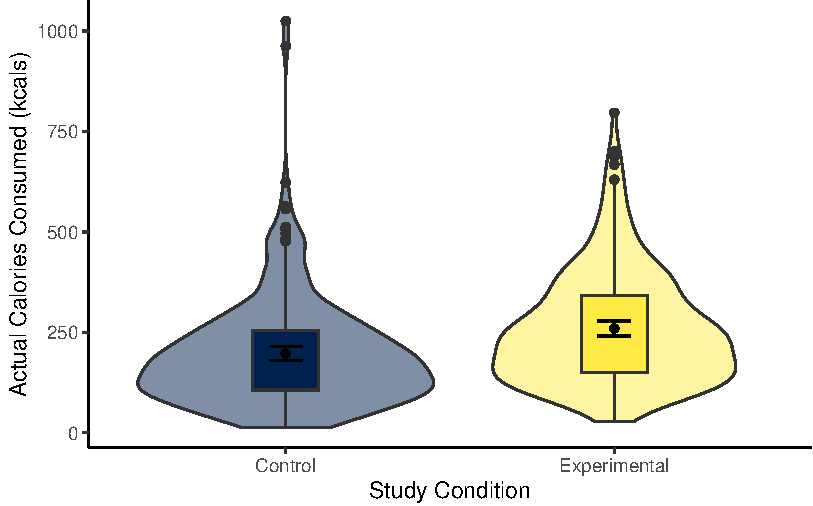
\includegraphics[width=1\textwidth,height=\textheight]{09-lm-categorical_files/figure-pdf/unnamed-chunk-38-1.pdf}
\end{center}

Our model explained a statistically significant amount of variance in
our outcome (adjusted \(R^2\) = .047, F(1, 462) = 23.64, \emph{p}
\textless{} .001). Condition was a positive predictor, where the
experimental group consumed on average 63 more calories than the control
group (\(b_1\) = 63.05, 95\% CI = {[}37.57, 88.53{]}, \emph{p}
\textless{} .001). Expressed as a standardised effect size, the
experimental group consumed 0.44 (95\% CI = {[}0.26, 0.62{]}) more
standard deviations than the control group.''

Note: we have not included an APA formatted Figure title here as it is
not easy to format in our book, so refer to the course materials for
guidance.

\subsection{Formatting your results
reproducibly}\label{formatting-your-results-reproducibly-1}

Like Chapter 8, we can also make regression models reproducible to add
into your reports. For regression models, the first step is saving your
model as an object \emph{before} you apply the \texttt{summary()}
function. We created this in activity 8, but as a reminder:

\begin{Shaded}
\begin{Highlighting}[]
\NormalTok{lm\_cals\_numbers }\OtherTok{\textless{}{-}} \FunctionTok{lm}\NormalTok{(}\AttributeTok{formula =}\NormalTok{ F\_CaloriesConsumed }\SpecialCharTok{\textasciitilde{}}\NormalTok{ Condition, }
                      \AttributeTok{data =}\NormalTok{ lopez\_clean)}
\end{Highlighting}
\end{Shaded}

To make the reporting flexible, we then separate the model into two
components: the overall model and the slope. For the overall model, you
must save the reporting function first. Note these are the exact same
functions as Chapter 8, so you would not need to duplicate them if you
already included them in a file.

\begin{Shaded}
\begin{Highlighting}[]
\NormalTok{report\_regression\_model }\OtherTok{\textless{}{-}} \ControlFlowTok{function}\NormalTok{(regression\_object)\{}
  \CommentTok{\# This function will only work for lm() objects}
  \CommentTok{\# Step 1 = apply the summary function so we have both objects}
\NormalTok{  model\_summary }\OtherTok{\textless{}{-}} \FunctionTok{summary}\NormalTok{(regression\_object)}
  \CommentTok{\# Step 2 = save all the numbers with formatting }
  \CommentTok{\# Save adjusted R2 with any trailing zeroes}
\NormalTok{  adj\_r2 }\OtherTok{\textless{}{-}} \FunctionTok{sprintf}\NormalTok{(}\StringTok{"\%.3f"}\NormalTok{, }\FunctionTok{round}\NormalTok{(model\_summary}\SpecialCharTok{$}\NormalTok{adj.r.squared, }\DecValTok{3}\NormalTok{))}
  \CommentTok{\# save model degrees of freedom}
\NormalTok{  df1 }\OtherTok{\textless{}{-}}\NormalTok{ model\_summary}\SpecialCharTok{$}\NormalTok{df[}\DecValTok{1}\NormalTok{]}
  \CommentTok{\# save residual degrees of freedom}
\NormalTok{  df2 }\OtherTok{\textless{}{-}}\NormalTok{ model\_summary}\SpecialCharTok{$}\NormalTok{df[}\DecValTok{2}\NormalTok{]}
  \CommentTok{\# save F rounded to 2 decimals with any trailing zeroes}
\NormalTok{  Fval }\OtherTok{\textless{}{-}} \FunctionTok{sprintf}\NormalTok{(}\StringTok{"\%.2f"}\NormalTok{, }\FunctionTok{round}\NormalTok{(model\_summary}\SpecialCharTok{$}\NormalTok{fstatistic, }\DecValTok{2}\NormalTok{))[}\DecValTok{1}\NormalTok{]}
  \CommentTok{\# save p value with formatting if less than .001}
\NormalTok{  pval }\OtherTok{\textless{}{-}} \FunctionTok{anova}\NormalTok{(regression\_object)}\SpecialCharTok{$}\StringTok{\textasciigrave{}}\AttributeTok{Pr(\textgreater{}F)}\StringTok{\textasciigrave{}}\NormalTok{[}\DecValTok{1}\NormalTok{]}
  \ControlFlowTok{if}\NormalTok{ (pval }\SpecialCharTok{\textgreater{}=} \FloatTok{0.001}\NormalTok{)\{}
\NormalTok{    pval }\OtherTok{\textless{}{-}} \FunctionTok{str\_sub}\NormalTok{(}\FunctionTok{as.character}\NormalTok{(pval), }\DecValTok{2}\NormalTok{, }\DecValTok{5}\NormalTok{)}
\NormalTok{    pval }\OtherTok{\textless{}{-}}  \FunctionTok{paste0}\NormalTok{(}\StringTok{", *p* = "}\NormalTok{, pval)}
  \CommentTok{\# If p \textless{} .001, manually format as p \textless{} .001}
\NormalTok{  \} }\ControlFlowTok{else} \ControlFlowTok{if}\NormalTok{ (pval }\SpecialCharTok{\textless{}} \FloatTok{0.001}\NormalTok{)\{}
\NormalTok{    pval }\OtherTok{\textless{}{-}} \StringTok{", *p* \textless{} .001"}
\NormalTok{  \}}

  \CommentTok{\# Step 3 = add them together in APA format}
\NormalTok{  output }\OtherTok{\textless{}{-}} \FunctionTok{paste0}\NormalTok{(}\StringTok{"adjusted $R\^{}2$ = "}\NormalTok{,}
\NormalTok{                   adj\_r2,}
                   \StringTok{", "}\NormalTok{,}
                   \StringTok{"F("}\NormalTok{, df1, }\StringTok{", "}\NormalTok{, df2, }\StringTok{") = "}\NormalTok{, Fval,}
\NormalTok{                   pval)}
  
  \FunctionTok{return}\NormalTok{(output)}
\NormalTok{\}}
\end{Highlighting}
\end{Shaded}

Then you can run the function on your regression model.

\begin{Shaded}
\begin{Highlighting}[]
\FunctionTok{report\_regression\_model}\NormalTok{(lm\_cals\_numbers)}
\end{Highlighting}
\end{Shaded}

\begin{verbatim}
[1] "adjusted $R^2$ = 0.047, F(2, 462) = 23.64, *p* < .001"
\end{verbatim}

For the slope, there is a separate reporting function.

\begin{Shaded}
\begin{Highlighting}[]
\NormalTok{report\_regression\_slope }\OtherTok{\textless{}{-}} \ControlFlowTok{function}\NormalTok{(regression\_object)\{}
  \CommentTok{\# This function will only work for lm() objects}
  \CommentTok{\# Step 1 = apply the summary function so we have both objects}
\NormalTok{  model\_summary }\OtherTok{\textless{}{-}} \FunctionTok{summary}\NormalTok{(regression\_object)}
  \CommentTok{\# Step 2 = save all the numbers with formatting }
  \CommentTok{\# $b\_1 = {-}0.40$, 95\% CI = [{-}0.44, {-}0.35], *p* \textless{} .001)}
  \CommentTok{\# Save slope with any trailing zeroes}
\NormalTok{  b\_1 }\OtherTok{\textless{}{-}} \FunctionTok{sprintf}\NormalTok{(}\StringTok{"\%.2f"}\NormalTok{, }\FunctionTok{round}\NormalTok{(model\_summary}\SpecialCharTok{$}\NormalTok{coefficients[}\DecValTok{2}\NormalTok{, }\DecValTok{1}\NormalTok{], }\DecValTok{2}\NormalTok{))}
  \CommentTok{\# save p value with formatting if less than .001}
\NormalTok{  pval }\OtherTok{\textless{}{-}}\NormalTok{ model\_summary}\SpecialCharTok{$}\NormalTok{coefficients[}\DecValTok{2}\NormalTok{, }\DecValTok{4}\NormalTok{]}
  \ControlFlowTok{if}\NormalTok{ (pval }\SpecialCharTok{\textgreater{}=} \FloatTok{0.001}\NormalTok{)\{}
\NormalTok{    pval }\OtherTok{\textless{}{-}} \FunctionTok{str\_sub}\NormalTok{(}\FunctionTok{as.character}\NormalTok{(pval), }\DecValTok{2}\NormalTok{, }\DecValTok{5}\NormalTok{)}
\NormalTok{    pval }\OtherTok{\textless{}{-}}  \FunctionTok{paste0}\NormalTok{(}\StringTok{", *p* = "}\NormalTok{, pval)}
  \CommentTok{\# If p \textless{} .001, manually format as p \textless{} .001}
\NormalTok{  \} }\ControlFlowTok{else} \ControlFlowTok{if}\NormalTok{ (pval }\SpecialCharTok{\textless{}} \FloatTok{0.001}\NormalTok{)\{}
\NormalTok{    pval }\OtherTok{\textless{}{-}} \StringTok{", *p* \textless{} .001"}
\NormalTok{  \}}
  \CommentTok{\# save lower 95\% CI}
\NormalTok{  lower\_CI }\OtherTok{\textless{}{-}} \FunctionTok{round}\NormalTok{(}\FunctionTok{confint}\NormalTok{(regression\_object)[}\DecValTok{2}\NormalTok{, }\DecValTok{1}\NormalTok{], }\DecValTok{2}\NormalTok{)}
  \CommentTok{\# save lower 95\% CI}
\NormalTok{  upper\_CI }\OtherTok{\textless{}{-}} \FunctionTok{round}\NormalTok{(}\FunctionTok{confint}\NormalTok{(regression\_object)[}\DecValTok{2}\NormalTok{, }\DecValTok{2}\NormalTok{], }\DecValTok{2}\NormalTok{)}
  \CommentTok{\# Switch CIs depending on sign }
\NormalTok{  b1\_CI }\OtherTok{\textless{}{-}} \FunctionTok{ifelse}\NormalTok{(b\_1 }\SpecialCharTok{\textgreater{}} \DecValTok{0}\NormalTok{,}
                 \FunctionTok{paste0}\NormalTok{(lower\_CI, }\StringTok{", "}\NormalTok{, upper\_CI),}
                 \FunctionTok{paste0}\NormalTok{(upper\_CI, }\StringTok{", "}\NormalTok{, lower\_CI))}
  
  \CommentTok{\# Step 3 = add them together in APA format}
\NormalTok{  output }\OtherTok{\textless{}{-}} \FunctionTok{paste0}\NormalTok{(}\StringTok{"$b\_1$ = "}\NormalTok{,}
\NormalTok{                   b\_1,}
                   \StringTok{", 95\% CI = ["}\NormalTok{, b1\_CI, }\StringTok{"]"}\NormalTok{,}
\NormalTok{                   pval)}
  
  \FunctionTok{return}\NormalTok{(output)}
\NormalTok{\}}
\end{Highlighting}
\end{Shaded}

Then you can run the function on your regression model.

\begin{Shaded}
\begin{Highlighting}[]
\FunctionTok{report\_regression\_slope}\NormalTok{(lm\_cals\_numbers)}
\end{Highlighting}
\end{Shaded}

\begin{verbatim}
[1] "$b_1$ = 63.05, 95% CI = [37.57, 88.53], *p* < .001"
\end{verbatim}

\section{Bonus section - One- and paired-samples tests}\label{09-bonus}

In this course, we focus on correlational and between-subjects designs,
but you might find yourself in a situation where you want to test a
continuous variable against a fixed value or compare conditions in the
same participants. This is a bonus section if you have time, so you can
skip to the \hyperref[09-test]{Test Yourself} section to finish the
chapter if you do not.

For this demonstration, we will use data from experiment 1 of Bem
(2011), an (in)famous study that almost single-handedly started the
replication crisis in psychology. Briefly, participants completed a
computer task adapted from priming experiments where they could select
one of two windows. They had to guess which window had an image hidden
behind it and the images contained different stimuli like erotic or
neutral/control images. Across many trials of the participants guessing
the location, Bem calculated the proportion of successful trials which
could range between 0 (never correct), 50 (50\%, chance), and 100
(always correct). The headline finding was participants demonstrated
precognition - or the ability to see into the future - to guess above
chance levels, but what does the data look like?

We are working with a new data set, so please save the following data
file: \href{data/Bem_2011.csv}{Bem\_2011.csv}. Right click the link and
select ``save link as'', or clicking the link will save the files to
your Downloads. Make sure that you save the file as ``.csv''. Save or
copy the file to your \texttt{data/} folder within
\texttt{Chapter\_09\_regression\_categorical}. Read in the data file to
the object \texttt{bem\_data} to be consistent with the tasks below.

\subsection{One-sample comparing against a fixed
value}\label{one-sample-comparing-against-a-fixed-value}

There are scenarios where you want to compare a single continuous
variable against a fixed value. For example, do your participants
respond significantly above or below chance?

\subsubsection{Expressed as a t-test}\label{expressed-as-a-t-test}

As a t-test, we need to specify two arguments:

\begin{itemize}
\item
  \texttt{x} - This is the continuous variable you want to analyse and
  compare the mean value of. We must use the base R operator \texttt{\$}
  to specify the column from your data.
\item
  \texttt{mu} - This is the fixed value you want to test your variable
  against.
\end{itemize}

In this scenario, we want to compare the hit rate to erotic images
against a value of 50. This will tell us if the hit rate is
significantly above or below chance.

\begin{Shaded}
\begin{Highlighting}[]
\FunctionTok{t.test}\NormalTok{(}\AttributeTok{x =}\NormalTok{ bem\_data}\SpecialCharTok{$}\NormalTok{Erotic.Hits.PC,}
       \AttributeTok{mu =} \DecValTok{50}\NormalTok{)}
\end{Highlighting}
\end{Shaded}

\begin{verbatim}

    One Sample t-test

data:  bem_data$Erotic.Hits.PC
t = 2.5133, df = 99, p-value = 0.01358
alternative hypothesis: true mean is not equal to 50
95 percent confidence interval:
 50.66075 55.61703
sample estimates:
mean of x 
 53.13889 
\end{verbatim}

The output is similar to the independent samples t-test. We get the
\emph{p}-value for hypothesis testing, the mean estimate of the
variable, and it's 95\% confidence interval. To express it as an effect
size, you can subtract 50 from each value. So, participants responded
3.14\% above chance, statistically significant, but hardly convincing
evidence for precognition.

\subsubsection{Expressed as a linear
model}\label{expressed-as-a-linear-model}

We can also express this as a linear model, but we must first add a
small wrangling step. In the one-sample t-test, we can manually enter a
fixed value to compare the mean against. In a linear model, we must
compare against 0 by subtracting the fixed value from your variable. So,
we subtract 50 from all the observations, so they become a kind of
deviation from 50.

\begin{Shaded}
\begin{Highlighting}[]
\NormalTok{bem\_data }\OtherTok{\textless{}{-}}\NormalTok{ bem\_data }\SpecialCharTok{\%\textgreater{}\%} 
  \FunctionTok{mutate}\NormalTok{(}\AttributeTok{erotic\_deviation =}\NormalTok{ Erotic.Hits.PC }\SpecialCharTok{{-}} \DecValTok{50}\NormalTok{)}
\end{Highlighting}
\end{Shaded}

In contrast to previous linear models, we only add a fixed intercept and
do not add a predictor. This recreates the one-sample t-test by
estimating the mean value of your outcome.

\begin{Shaded}
\begin{Highlighting}[]
\NormalTok{lm\_erotic }\OtherTok{\textless{}{-}} \FunctionTok{lm}\NormalTok{(erotic\_deviation }\SpecialCharTok{\textasciitilde{}} \DecValTok{1}\NormalTok{, }
                \AttributeTok{data =}\NormalTok{ bem\_data)}

\FunctionTok{summary}\NormalTok{(lm\_erotic)}
\end{Highlighting}
\end{Shaded}

\begin{verbatim}

Call:
lm(formula = erotic_deviation ~ 1, data = bem_data)

Residuals:
    Min      1Q  Median      3Q     Max 
-28.139  -8.694   2.417   7.972  30.194 

Coefficients:
            Estimate Std. Error t value Pr(>|t|)  
(Intercept)    3.139      1.249   2.513   0.0136 *
---
Signif. codes:  0 '***' 0.001 '**' 0.01 '*' 0.05 '.' 0.1 ' ' 1

Residual standard error: 12.49 on 99 degrees of freedom
\end{verbatim}

This process has the benefit of directly producing your effect size, as
the intercept estimate is the deviation from your fixed value (here,
50). As we calculated manually before, the erotic hit rate is 3.14\%
above your fixed value. If you remember back to the linear model
explanations, this is where the \emph{p}-value for the intercept is
finally useful as it tests against 0.

If you compare to the one-sample t-test, all of these values are
identical. You also have the option of calculating confidence intervals
around the estimate, calculating a standardised effect size, and
checking assumptions by applying the previous linear regression
activities.

\subsection{Paired-samples comparing
conditions}\label{paired-samples-comparing-conditions}

Alternatively, you might want to compare two conditions from the same
participants in paired samples/within-subjects design. For example, is
the hit-rate significantly higher for erotic images compared to control
images?

\subsubsection{Expressed as a t-test}\label{expressed-as-a-t-test-1}

To conduct a paired-samples t-test, we must specify three arguments:

\begin{itemize}
\item
  \texttt{x} - This is the first level of your condition as a column.
  You need your data in wide format, so the condition levels are spread
  across two columns per participant. We must use the base R operator
  \texttt{\$} to specify the column from your data.
\item
  \texttt{y} - This is the second level of your condition as a column.
\item
  \texttt{paired} - This instructs R you want a paired-samples t-test to
  compare conditions within participants.
\end{itemize}

In this scenario, we want to compare the hit rate for erotic images to
control images.

\begin{Shaded}
\begin{Highlighting}[]
\FunctionTok{t.test}\NormalTok{(}\AttributeTok{x =}\NormalTok{ bem\_data}\SpecialCharTok{$}\NormalTok{Erotic.Hits.PC,}
       \AttributeTok{y =}\NormalTok{ bem\_data}\SpecialCharTok{$}\NormalTok{Control.Hits.PC, }
       \AttributeTok{paired =} \ConstantTok{TRUE}\NormalTok{)}
\end{Highlighting}
\end{Shaded}

\begin{verbatim}

    Paired t-test

data:  bem_data$Erotic.Hits.PC and bem_data$Control.Hits.PC
t = 1.8563, df = 99, p-value = 0.06638
alternative hypothesis: true mean difference is not equal to 0
95 percent confidence interval:
 -0.2277431  6.8388542
sample estimates:
mean difference 
       3.305556 
\end{verbatim}

The output is almost identical to the one-sample t-test, but this time
the effect size is the mean difference between conditions, not just the
mean per condition. Behind the scenes, a paired-samples t-test is
actually a one-sample t-test in disguise as it uses the difference
between conditions as the outcome.

As an aside, Bem (2011) reported a significant difference here, but only
because he reported a one-tailed test
(\texttt{alternative\ =\ "greater"}). This is an example where you
ideally need a strong (ideally pre-registered) prediction as it makes a
material impact on the inferences you would make.

\subsubsection{Expressed as a linear
model}\label{expressed-as-a-linear-model-1}

Finally, we can express a paired-samples t-test as a linear model. We
must apply a small data wrangling step to calculate a difference score
between conditions. This is so the linear model compares the estimate
against 0 of no difference. So, for this example, we create a variable
for the difference between erotic and control images.

\begin{Shaded}
\begin{Highlighting}[]
\NormalTok{bem\_data }\OtherTok{\textless{}{-}}\NormalTok{ bem\_data }\SpecialCharTok{\%\textgreater{}\%} 
  \FunctionTok{mutate}\NormalTok{(}\AttributeTok{erotic\_control =}\NormalTok{ Erotic.Hits.PC }\SpecialCharTok{{-}}\NormalTok{ Control.Hits.PC)}
\end{Highlighting}
\end{Shaded}

Like the one-sample scenario, we only add a fixed intercept for the new
difference variance and do not add a predictor. This recreates the
paired-samples t-test by estimating the mean value of your difference
score.

\begin{Shaded}
\begin{Highlighting}[]
\NormalTok{lm\_paired }\OtherTok{\textless{}{-}} \FunctionTok{lm}\NormalTok{(erotic\_control }\SpecialCharTok{\textasciitilde{}} \DecValTok{1}\NormalTok{, }
                \AttributeTok{data =}\NormalTok{ bem\_data)}

\FunctionTok{summary}\NormalTok{(lm\_paired)}
\end{Highlighting}
\end{Shaded}

\begin{verbatim}

Call:
lm(formula = erotic_control ~ 1, data = bem_data)

Residuals:
    Min      1Q  Median      3Q     Max 
-58.861  -9.556   2.250   9.194  35.583 

Coefficients:
            Estimate Std. Error t value Pr(>|t|)  
(Intercept)    3.306      1.781   1.856   0.0664 .
---
Signif. codes:  0 '***' 0.001 '**' 0.01 '*' 0.05 '.' 0.1 ' ' 1

Residual standard error: 17.81 on 99 degrees of freedom
\end{verbatim}

This process directly produces your effect size again, as the intercept
estimate is the deviation from 0 for your difference score. As we saw in
the paired-samples t-test output, there was a 3.31\% higher hit rate for
erotic images compared to control (as we calculated erotic - control).

If you compare to the paired-samples t-test, all of these values are
identical. You also have the option of calculating confidence intervals
around the estimate, calculating a standardised effect size, and
checking assumptions by applying the previous linear regression
activities.

\section{Test Yourself}\label{09-test}

To end the chapter, we have some knowledge check questions to test your
understanding of the concepts we covered in the chapter. Compared to
previous chapters, there are no error mode questions as the content is
so similar to Chapter 8. We are just going to test your understanding of
the concepts rather than potential errors.

\subsection{Knowledge check}\label{knowledge-check-8}

For this chapter's knowledge check section, we have something a little
different. Instead of purely conceptual questions about functions, we
have another example of linear regression from Lopez et al. (2023). Feel
free to create this model yourself, but we will show you some output and
ask you questions based on it.

For this model, we focus on ounces of soup consumed
(\texttt{M\_postsoup}) rather than calories by each Condition group
(\texttt{Condition\_label}). You might have a good idea about the
results based on the chapter, but you will still need to interpret the
output accurately.

\textbf{Question 1}. In the violin-boxplot below, the experimental group
consumed more soup in ounces than the control group: TRUE / FALSE.

\begin{center}
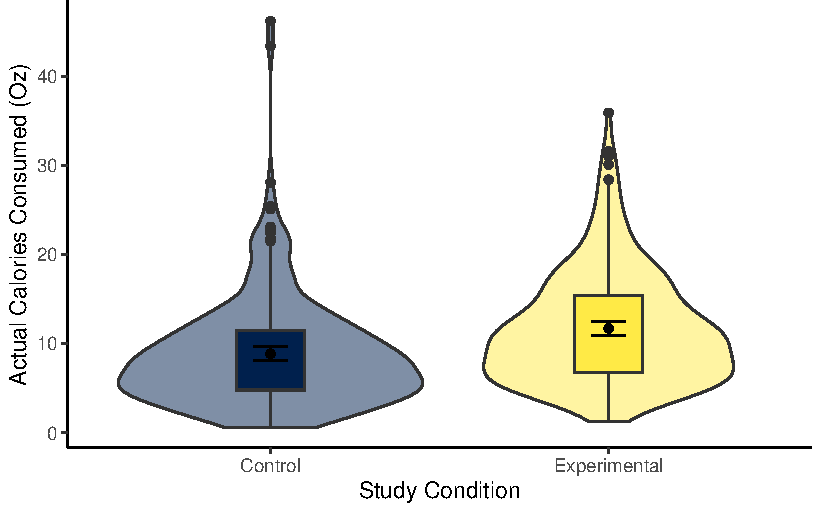
\includegraphics[width=1\textwidth,height=\textheight]{09-lm-categorical_files/figure-pdf/unnamed-chunk-51-1.pdf}
\end{center}

\textbf{Question 2} For the next few questions, we have the output from
a linear regression model and we would like you to interpret it.

\begin{verbatim}

Call:
lm(formula = M_postsoup ~ Condition_label, data = lopez_clean)

Residuals:
    Min      1Q  Median      3Q     Max 
-10.410  -4.467  -1.089   2.833  37.333 

Coefficients:
                            Estimate Std. Error t value Pr(>|t|)    
(Intercept)                   8.8675     0.4007  22.130  < 2e-16 ***
Condition_labelExperimental   2.8426     0.5846   4.863 1.59e-06 ***
---
Signif. codes:  0 '***' 0.001 '**' 0.01 '*' 0.05 '.' 0.1 ' ' 1

Residual standard error: 6.285 on 462 degrees of freedom
Multiple R-squared:  0.04869,   Adjusted R-squared:  0.04663 
F-statistic: 23.64 on 1 and 462 DF,  p-value: 1.591e-06
\end{verbatim}

The outcome variable in this model is

\begin{itemize}
\tightlist
\item
  \begin{enumerate}
  \def\labelenumi{(\Alph{enumi})}
  \tightlist
  \item
    Actual ounces of soup consumed\\
  \end{enumerate}
\item
  \begin{enumerate}
  \def\labelenumi{(\Alph{enumi})}
  \setcounter{enumi}{1}
  \tightlist
  \item
    Experimental condition
  \end{enumerate}
\end{itemize}

and the predictor variable is

\begin{itemize}
\tightlist
\item
  \begin{enumerate}
  \def\labelenumi{(\Alph{enumi})}
  \tightlist
  \item
    Actual ounces of soup consumed\\
  \end{enumerate}
\item
  \begin{enumerate}
  \def\labelenumi{(\Alph{enumi})}
  \setcounter{enumi}{1}
  \tightlist
  \item
    Experimental condition
  \end{enumerate}
\end{itemize}

.

\textbf{Question 3} In this model, the reference group is

\begin{itemize}
\tightlist
\item
  \begin{enumerate}
  \def\labelenumi{(\Alph{enumi})}
  \tightlist
  \item
    Control\\
  \end{enumerate}
\item
  \begin{enumerate}
  \def\labelenumi{(\Alph{enumi})}
  \setcounter{enumi}{1}
  \tightlist
  \item
    Experimental
  \end{enumerate}
\end{itemize}

and the target group is

\begin{itemize}
\tightlist
\item
  \begin{enumerate}
  \def\labelenumi{(\Alph{enumi})}
  \tightlist
  \item
    Control\\
  \end{enumerate}
\item
  \begin{enumerate}
  \def\labelenumi{(\Alph{enumi})}
  \setcounter{enumi}{1}
  \tightlist
  \item
    Experimental
  \end{enumerate}
\end{itemize}

\textbf{Question 4} Rounded to 2 decimals, we predict a value of
\_\_\_\_ for our reference group.

\textbf{Question 5} The predictor is

\begin{itemize}
\tightlist
\item
  \begin{enumerate}
  \def\labelenumi{(\Alph{enumi})}
  \tightlist
  \item
    statistically significant\\
  \end{enumerate}
\item
  \begin{enumerate}
  \def\labelenumi{(\Alph{enumi})}
  \setcounter{enumi}{1}
  \tightlist
  \item
    non-significant
  \end{enumerate}
\end{itemize}

and

\begin{itemize}
\tightlist
\item
  \begin{enumerate}
  \def\labelenumi{(\Alph{enumi})}
  \tightlist
  \item
    positive\\
  \end{enumerate}
\item
  \begin{enumerate}
  \def\labelenumi{(\Alph{enumi})}
  \setcounter{enumi}{1}
  \tightlist
  \item
    negative
  \end{enumerate}
\end{itemize}

.

\textbf{Question 6} The target group consumed on average \_\_\_\_ ounces

\begin{itemize}
\tightlist
\item
  \begin{enumerate}
  \def\labelenumi{(\Alph{enumi})}
  \tightlist
  \item
    less\\
  \end{enumerate}
\item
  \begin{enumerate}
  \def\labelenumi{(\Alph{enumi})}
  \setcounter{enumi}{1}
  \tightlist
  \item
    more
  \end{enumerate}
\end{itemize}

soup than the reference group.

\section{Words from this Chapter}\label{words-from-this-chapter-8}

Below you will find a list of words that were used in this chapter that
might be new to you in case it helps to have somewhere to refer back to
what they mean. The links in this table take you to the entry for the
words in the \href{https://psyteachr.github.io/glossary/}{PsyTeachR
Glossary}. Note that the Glossary is written by numerous members of the
team and as such may use slightly different terminology from that shown
in the chapter.

\begin{longtable}[]{@{}
  >{\raggedright\arraybackslash}p{(\columnwidth - 2\tabcolsep) * \real{0.1938}}
  >{\raggedright\arraybackslash}p{(\columnwidth - 2\tabcolsep) * \real{0.8062}}@{}}
\toprule\noalign{}
\begin{minipage}[b]{\linewidth}\raggedright
term
\end{minipage} & \begin{minipage}[b]{\linewidth}\raggedright
definition
\end{minipage} \\
\midrule\noalign{}
\endhead
\bottomrule\noalign{}
\endlastfoot
\href{https://psyteachr.github.io/glossary/d\#dummy-coding}{dummy-coding}
& Entering a categorical predictor using two values such as 0 and 1. \\
\href{https://psyteachr.github.io/glossary/r\#reference-group}{reference-group}
& In a dummy-coded variable, the first level of your variable, typically
0. \\
\href{https://psyteachr.github.io/glossary/s\#student-t-test}{student-t-test}
& Calculating a t-value based on the mean difference divided by the
pooled standard deviation. In the Student t-test, we times the pooled
standard deviation by a term containing the sample sizes of each
group. \\
\href{https://psyteachr.github.io/glossary/t\#target-group}{target-group}
& In a dummy-coded variable, the second level of your variable,
typically 1. \\
\href{https://psyteachr.github.io/glossary/w\#welch-t-test}{welch-t-test}
& Calculating a t-value based on the mean difference divided by a term
containing the variance of each group. We also correct the degrees of
freedom for the difference in variances. \\
\end{longtable}

\section{End of chapter}\label{end-of-chapter-8}

Well done, you have now completed the first core set of chapters for
inferential statistics!

At this point, you can now address a range of research questions by
applying variations of the general linear model. As a researcher, the
most important thing is starting with your research question (and where
applicable, your hypothesis), designing a study to address that research
question, and using an appropriate statistical model for your design and
research question. But, before you can identify an appropriate
statistical model, you need to know what they look like! This is
everything we cover in Research Methods 1 to focus on a select range of
foundational skills. You will then build on these modelling techniques
in Chapters 12-14 for Research Methods 2.

You are now ready to complete the second data analysis journey chapter:
\hyperref[journey-02-wrangling]{Simple Linear Regression}. This is where
you can test your new skills in a slightly less structured way, from
wrangling data, to answering a research question.

In the next core chapter, we turn to statistical power and work on how
you can conduct a power analysis in R/RStudio.

\bookmarksetup{startatroot}

\chapter{Statistical Power and Effect
Sizes}\label{statistical-power-and-effect-sizes}

Until now, a large component of each chapter was dedicated to data
wrangling as we must first process raw data into something tidier we can
apply our visualisation or modelling steps to. In this chapter, there is
no data wrangling, just functions to calculate statistical power in
different ways for different tests. Before, the difficulty was in unique
problems in wrangling your specific data. In power analysis, the
functions are pretty straight forward to use, but deciding what inputs
you use are the hard parts as they are your decisions to make.

We adapted a few components of this chapter from J. Bartlett \& Charles
(2022) and we recommend referring to this article for more information
on the concepts behind statistical power. However, the article focuses
on the statistics software jamovi, so this chapter focuses on power
analysis using the pwr package.

\textbf{Chapter Intended Learning Outcomes (ILOs)}

By the end of this chapter, you will be able to:

\begin{itemize}
\item
  Conduct and interpret an \emph{a priori} power analysis for t-tests,
  correlations, and regression models.
\item
  Conduct and interpret a sensitivity power analysis for t-tests,
  correlations, and regression models.
\item
  Report your power analysis to make it reproducible for your reader.
\end{itemize}

\section{Chapter preparation}\label{chapter-preparation-7}

\subsection{Organising your files and project for the
chapter}\label{organising-your-files-and-project-for-the-chapter-7}

In contrast to previous chapters, there will be no data wrangling in
this chapter, so we do not need to worry about downloading files. We
will still be working around some key studies, but we will introduce
them as needed. However, you will still be working in an R Markdown
document, so you need to make sure your working directory is in order.

\begin{enumerate}
\def\labelenumi{\arabic{enumi}.}
\item
  In your folder for research methods and the book
  \texttt{ResearchMethods1\_2/Quant\_Fundamentals}, create a new folder
  called \texttt{Chapter\_10\_power}.
\item
  Create an R Project for \texttt{Chapter\_10\_power} as an existing
  directory for your chapter folder. This should now be your working
  directory.
\item
  Create a new R Markdown document and give it a sensible title
  describing the chapter, such as
  \texttt{10\ Statistical\ Power\ and\ Effect\ Sizes}. Delete everything
  below line 10 so you have a blank file to work with and save the file
  in your \texttt{Chapter\_10\_power} folder.
\item
  In a code chunk, load the pwr and tidyverse packages. If you need to
  install any packages, revisit \hyperref[install-tidy]{Chapter 1} if
  you need a refresher, but remember not to install packages on the
  university computers / online server.
\end{enumerate}

You are now ready to start working on the chapter!

\section{NHST and statistical power
recap}\label{nhst-and-statistical-power-recap}

Given there is no data wrangling for this chapter and the functions for
power analysis are pretty straight forward, we have a little space to
recap the key concepts behind power analysis. Almost all the work here
comes into thinking and justifying your decisions, rather than spending
lots of time on wrangling and analysis.

The branch of statistics we are using here is Null Hypothesis
Significance Testing (NHST). There are two types of hypotheses and what
you are trying to establish is the probability of rejecting the null
hypothesis. Those two hypotheses are:

\begin{itemize}
\tightlist
\item
  The \textbf{null hypothesis} which states that there is no difference
  (\(H_0: \mu_1 = \mu_2\)) or no relationship (\(H_0: r = 0\)).
\item
  The \textbf{alternative hypothesis} which states that there is a
  difference (\(H_1: \mu_1 \ne \mu_2\)) or there is a relationship
  (\(H_1: r \ne 0\)).
\end{itemize}

NHST is designed to control error rates associated with two main
decisions around these hypotheses:

\begin{itemize}
\item
  \textbf{Type I error} - or false positive, is the probability of
  rejecting the null hypothesis when it should not be rejected
  (otherwise called alpha or \(\alpha\)). In other words, you conclude
  that there is a real ``effect'' when in fact there is no effect. The
  field standard rate of acceptable false positives is \(\alpha = .05\),
  meaning that we would accept 1 in 20 studies may be a false positive.
\item
  \textbf{Type II error} - or false negative, is the probability of
  retaining the null hypothesis when it should be rejected (otherwise
  called beta or \(\beta\)). In other words, you conclude that there was
  no real ``effect'' when in fact there was one. There is less tradition
  around this, but the most common rule of thumb you will come across is
  \(\beta = .20\), meaning that we would accept 1 in 5 studies may be a
  false negative.
\end{itemize}

Statistical power is the opposite of beta and represents the long-run
probability of correctly rejecting the null hypothesis when there is a
real effect to detect. In other words, how likely are you to detect an
effect that is really there? You calculate Power as \(1-\beta\), meaning
that if the field standard for beta is \(\beta = .20\), then the field
standard for power is \(1 - .20 = .80\) (80\%).

In addition to alpha and beta/power, there are two other key concepts
(there are more depending on the test, but we will add them in when we
need them):

\begin{itemize}
\item
  \textbf{Effect size} - A number that expresses the magnitude of the
  phenomenon relevant to your research question. In Chapters 8 and 9, we
  introduced you to different standardised effect sizes such as
  Pearson's \emph{r} and Cohen's d.~
\item
  \textbf{Sample size} - The number of observations (usually
  participants, but it might be animals or stimuli depending on your
  topic) in your study.
\end{itemize}

Critically, there is a relationship between these four concepts, where
if you know three, you can calculate the \textbf{fourth} in a process
called \textbf{power analysis}. The two most useful types of power
analysis are:

\begin{enumerate}
\def\labelenumi{\arabic{enumi}.}
\item
  \textbf{A priori} power analysis: How many participants do I need, for
  a given alpha, beta/power, and smallest effect size of interest? This
  is most useful in the design stage to help you plan how many
  participants you need to design an informative study.
\item
  \textbf{Sensitivity} power analysis: What effect size can I detect,
  for a given alpha, beta/power, and sample size? This is most useful
  after you finish collecting data or when you are using secondary data
  as the sample size is not longer under your control and it helps put
  your findings in context.
\end{enumerate}

You may now be thinking though, if there is a relationship between all
four concepts, could we calculate power for a given alpha, sample size,
and effect size? It is a tempting idea and you might see some articles
report it, but unfortunately is is misleading and tells you nothing more
than the \emph{p}-value does. The short version is we are typically
using a sample to learn something about a population, so there is
uncertainty in the estimate. Using the observed effect size in your
study assumes this is the true population effect, which is rarely a good
assumption. If you are interested, Lakens (2022) is a great resource for
sample size justification in general, but also explains why post-hoc
power is not a good idea.

After the brief recap, we will now focus on \emph{a priori} and
sensitivity power analyses applied to different statistical models.

\section{Power analysis for t-tests / categorical
predictors}\label{power-analysis-for-t-tests-categorical-predictors}

\subsection{Introduction to the study}\label{introduction-to-the-study}

In this section, imagine we are designing a study to build on Irving et
al. (2022) who tested an intervention to correct statistical
misinformation. Participants read an article about a new fictional study
where one passage falsely concludes watching TV causes cognitive
decline. In the correction group, participants receive an extra passage
where the fictional researcher explains they only reported a
correlation, not a causal relationship. In the no-correction group, the
extra passage just explains the fictional researcher was not available
to comment. Irving et al.~then tested participants' comprehension of the
story and coded their answers for mistaken causal inferences. They
expected participants in the correction group to make fewer causal
inferences than those in the no-correction group, and found evidence
supporting this prediction with an effect size equivalent to Cohen's d =
0.64, 95\% CI = {[}0.28, 0.99{]}. Inspired by their study, we want to
design an experiment to correct another type of misinformation in
articles.

Irving et al.~(2022) themselves provide an excellent example of
explaining and justifying the rationale behind their power analysis, so
we will walk through the decision making process and how it changes the
outputs. For our smallest effect size of interest, our starting point is
the estimate of d = 0.64. However, it is worth consulting other sources
to calibrate our understanding of effects in the area, such as Irving et
al.~citing a meta-analysis. For debunking, the average effect across 30
studies was d = 1.14, 95\% CI = {[}0.68, 1.61{]}, so we could use the
lower bound of the confidence interval, but this may still represent an
overestimate. Irving et al.~used the smallest effect (d = 0.54) from the
studies most similar to their design which was included in the
meta-analysis. As a value slightly smaller than the other estimates, we
will also use this as the smallest effect of interest for our study.

Now we have settled on our smallest effect size of interest, we will use
d = 0.54 in the following demonstrations. We start with \emph{a priori}
and sensitivity power analysis for two independent samples, exploring
how the outputs change as we alter inputs like alpha, power, and the
number of tails in the test.

\subsection{A priori power analysis}\label{a-priori-power-analysis}

For an independent samples t-test (we will cover regression shortly),
there is the function \texttt{pwr.t.test()}. We can enter the following
arguments:

\begin{itemize}
\item
  \texttt{n}: The number of observations.
\item
  \texttt{d}: The effect size as Cohen's d.~
\item
  \texttt{sig.level}: The alpha level.
\item
  \texttt{power}: The power value as 1-\(\beta\).
\item
  \texttt{type}: Whether you want power for a one-, paired-, or
  independant-samples t-test.
\item
  \texttt{alternative}: Whether you have a one- or two-sided hypothesis.
\end{itemize}

Remember, power analysis works by leaving one argument blank, so for
calculating the sample size, we leave \texttt{n} blank or enter
\texttt{NULL} as the argument. As our starting point, we enter d = 0.54,
sig.level = .05, power = .90, type = two.sample and alternative =
two-sided.

\begin{Shaded}
\begin{Highlighting}[]
\FunctionTok{pwr.t.test}\NormalTok{(}\AttributeTok{n =} \ConstantTok{NULL}\NormalTok{, }
           \AttributeTok{d =} \FloatTok{0.54}\NormalTok{, }
           \AttributeTok{sig.level =}\NormalTok{ .}\DecValTok{05}\NormalTok{, }
           \AttributeTok{power =}\NormalTok{ .}\DecValTok{90}\NormalTok{, }
           \AttributeTok{type =} \StringTok{"two.sample"}\NormalTok{, }
           \AttributeTok{alternative =} \StringTok{"two.sided"}\NormalTok{)}
\end{Highlighting}
\end{Shaded}

\begin{verbatim}

     Two-sample t test power calculation 

              n = 73.04123
              d = 0.54
      sig.level = 0.05
          power = 0.9
    alternative = two.sided

NOTE: n is number in *each* group
\end{verbatim}

As the note warns us, for an independent-samples t-test, \texttt{n}
represents the number of observations per group, so we need \textbf{74}
per group (we round up as we cannot have .04 of a person) or N =
\textbf{148}.

If you wanted to use these values in inline code, you can save the power
analysis object and pick out values to work with.

\begin{Shaded}
\begin{Highlighting}[]
\NormalTok{irving\_samplesize }\OtherTok{\textless{}{-}} \FunctionTok{pwr.t.test}\NormalTok{(}\AttributeTok{n =} \ConstantTok{NULL}\NormalTok{, }
                           \AttributeTok{d =} \FloatTok{0.54}\NormalTok{, }
                           \AttributeTok{sig.level =}\NormalTok{ .}\DecValTok{05}\NormalTok{, }
                           \AttributeTok{power =}\NormalTok{ .}\DecValTok{90}\NormalTok{, }
                           \AttributeTok{type =} \StringTok{"two.sample"}\NormalTok{, }
                           \AttributeTok{alternative =} \StringTok{"two.sided"}\NormalTok{) }\SpecialCharTok{\%\textgreater{}\%} 
  \FunctionTok{pluck}\NormalTok{(}\StringTok{"n"}\NormalTok{) }\SpecialCharTok{\%\textgreater{}\%} 
  \FunctionTok{ceiling}\NormalTok{()}
\end{Highlighting}
\end{Shaded}

In this code, we save the power analysis function to an object, use the
\texttt{pluck()} function to pick out a specific component (the argument
name must be spelt exactly), and use the \texttt{ceiling()} function to
round up. This helps to avoid manually calculating the values as you can
use the object.

\begin{Shaded}
\begin{Highlighting}[]
\CommentTok{\# sample size per group}
\NormalTok{irving\_samplesize}

\CommentTok{\# total sample size}
\NormalTok{irving\_samplesize }\SpecialCharTok{*} \DecValTok{2}
\end{Highlighting}
\end{Shaded}

\begin{verbatim}
[1] 74
[1] 148
\end{verbatim}

The power analysis function is pretty straight forward to work with, it
is the thinking and decision making that goes into selecting the value
for each argument that is the hardest part here. It is ultimately a
subjective decision you must be able to justify in a report and there
will always be compromises. You never have unlimited resources, so you
are trying to balance designing the most informative study with
maximizing the resources available to you.

\begin{tcolorbox}[enhanced jigsaw, breakable, colframe=quarto-callout-tip-color-frame, arc=.35mm, opacitybacktitle=0.6, titlerule=0mm, colbacktitle=quarto-callout-tip-color!10!white, colback=white, toprule=.15mm, bottomtitle=1mm, toptitle=1mm, title=\textcolor{quarto-callout-tip-color}{\faLightbulb}\hspace{0.5em}{Try this}, bottomrule=.15mm, rightrule=.15mm, leftrule=.75mm, coltitle=black, left=2mm, opacityback=0]

With decision making in mind, we can tweak the arguments to see how it
affects the sample size we need. We will tweak one argument at a time,
so your starting point will be the arguments we started with above.

\begin{enumerate}
\def\labelenumi{\arabic{enumi}.}
\item
  If we used a one-tailed test predicting a positive effect
  (\texttt{"greater"}), we would need \_\_ participants per group (N =
  \_\_\_).
\item
  If we wanted to make fewer type I errors and reduce alpha to .005, we
  would need \_\_\_ participants per group (N = \_\_\_).
\item
  If we were happy with a larger beta and reduce power to .80 (80\%), we
  would need \_\_ participants per group (N = \_\_\_).
\item
  If we wanted to decrease our smallest effect size of interest and set
  d = .40, we would need \_\_\_ participants per group (N = \_\_\_).
\item
  If we thought it was appropriate to change the design to
  within-subjects and use a paired-samples t-test instead
  (\texttt{"paired"}), we would need \_\_ participants.
\end{enumerate}

\end{tcolorbox}

\begin{tcolorbox}[enhanced jigsaw, breakable, colframe=quarto-callout-caution-color-frame, arc=.35mm, opacitybacktitle=0.6, titlerule=0mm, colbacktitle=quarto-callout-caution-color!10!white, colback=white, toprule=.15mm, bottomtitle=1mm, toptitle=1mm, title=\textcolor{quarto-callout-caution-color}{\faFire}\hspace{0.5em}{Show me the solution}, bottomrule=.15mm, rightrule=.15mm, leftrule=.75mm, coltitle=black, left=2mm, opacityback=0]

\begin{enumerate}
\def\labelenumi{\arabic{enumi}.}
\tightlist
\item
  We can calculate sample size for a one-tailed test by entering
  \texttt{alternative\ =\ "greater"} or \texttt{alternative\ =\ "less"}.
  This must match the effect size direction or you will receive an
  error.
\end{enumerate}

\begin{Shaded}
\begin{Highlighting}[]
\FunctionTok{pwr.t.test}\NormalTok{(}\AttributeTok{n =} \ConstantTok{NULL}\NormalTok{, }
           \AttributeTok{d =} \FloatTok{0.54}\NormalTok{, }
           \AttributeTok{sig.level =}\NormalTok{ .}\DecValTok{05}\NormalTok{, }
           \AttributeTok{power =}\NormalTok{ .}\DecValTok{90}\NormalTok{, }
           \AttributeTok{type =} \StringTok{"two.sample"}\NormalTok{, }
           \AttributeTok{alternative =} \StringTok{"greater"}\NormalTok{) }\SpecialCharTok{\%\textgreater{}\%} 
  \FunctionTok{pluck}\NormalTok{(}\StringTok{"n"}\NormalTok{) }\SpecialCharTok{\%\textgreater{}\%} 
  \FunctionTok{ceiling}\NormalTok{()}
\end{Highlighting}
\end{Shaded}

\begin{verbatim}
[1] 60
\end{verbatim}

\begin{enumerate}
\def\labelenumi{\arabic{enumi}.}
\setcounter{enumi}{1}
\tightlist
\item
  We can decrease alpha by entering \texttt{alpha\ =\ .005} to calculate
  the sample size for reducing the type I error rate.
\end{enumerate}

\begin{Shaded}
\begin{Highlighting}[]
\FunctionTok{pwr.t.test}\NormalTok{(}\AttributeTok{n =} \ConstantTok{NULL}\NormalTok{, }
           \AttributeTok{d =} \FloatTok{0.54}\NormalTok{, }
           \AttributeTok{sig.level =}\NormalTok{ .}\DecValTok{005}\NormalTok{, }
           \AttributeTok{power =}\NormalTok{ .}\DecValTok{90}\NormalTok{, }
           \AttributeTok{type =} \StringTok{"two.sample"}\NormalTok{, }
           \AttributeTok{alternative =} \StringTok{"two.sided"}\NormalTok{) }\SpecialCharTok{\%\textgreater{}\%} 
  \FunctionTok{pluck}\NormalTok{(}\StringTok{"n"}\NormalTok{) }\SpecialCharTok{\%\textgreater{}\%} 
  \FunctionTok{ceiling}\NormalTok{()}
\end{Highlighting}
\end{Shaded}

\begin{verbatim}
[1] 117
\end{verbatim}

\begin{enumerate}
\def\labelenumi{\arabic{enumi}.}
\setcounter{enumi}{2}
\tightlist
\item
  We can decrease power if we were happy with a larger beta / type II
  error rate by entering \texttt{power\ =\ .80}.
\end{enumerate}

\begin{Shaded}
\begin{Highlighting}[]
\FunctionTok{pwr.t.test}\NormalTok{(}\AttributeTok{n =} \ConstantTok{NULL}\NormalTok{, }
           \AttributeTok{d =} \FloatTok{0.54}\NormalTok{, }
           \AttributeTok{sig.level =}\NormalTok{ .}\DecValTok{05}\NormalTok{, }
           \AttributeTok{power =}\NormalTok{ .}\DecValTok{80}\NormalTok{, }
           \AttributeTok{type =} \StringTok{"two.sample"}\NormalTok{, }
           \AttributeTok{alternative =} \StringTok{"two.sided"}\NormalTok{) }\SpecialCharTok{\%\textgreater{}\%} 
  \FunctionTok{pluck}\NormalTok{(}\StringTok{"n"}\NormalTok{) }\SpecialCharTok{\%\textgreater{}\%} 
  \FunctionTok{ceiling}\NormalTok{()}
\end{Highlighting}
\end{Shaded}

\begin{verbatim}
[1] 55
\end{verbatim}

\begin{enumerate}
\def\labelenumi{\arabic{enumi}.}
\setcounter{enumi}{3}
\tightlist
\item
  We can decrease the smallest effect size of interest if we wanted the
  study to be more sensitive by entering \texttt{d\ =\ .40}.
\end{enumerate}

\begin{Shaded}
\begin{Highlighting}[]
\FunctionTok{pwr.t.test}\NormalTok{(}\AttributeTok{n =} \ConstantTok{NULL}\NormalTok{, }
           \AttributeTok{d =} \FloatTok{0.40}\NormalTok{, }
           \AttributeTok{sig.level =}\NormalTok{ .}\DecValTok{05}\NormalTok{, }
           \AttributeTok{power =}\NormalTok{ .}\DecValTok{90}\NormalTok{, }
           \AttributeTok{type =} \StringTok{"two.sample"}\NormalTok{, }
           \AttributeTok{alternative =} \StringTok{"two.sided"}\NormalTok{) }\SpecialCharTok{\%\textgreater{}\%} 
  \FunctionTok{pluck}\NormalTok{(}\StringTok{"n"}\NormalTok{) }\SpecialCharTok{\%\textgreater{}\%} 
  \FunctionTok{ceiling}\NormalTok{()}
\end{Highlighting}
\end{Shaded}

\begin{verbatim}
[1] 133
\end{verbatim}

\begin{enumerate}
\def\labelenumi{\arabic{enumi}.}
\setcounter{enumi}{4}
\tightlist
\item
  If we changed the design and test to within-subjects, we can enter
  \texttt{type\ =\ "paired"}.
\end{enumerate}

\begin{Shaded}
\begin{Highlighting}[]
\FunctionTok{pwr.t.test}\NormalTok{(}\AttributeTok{n =} \ConstantTok{NULL}\NormalTok{, }
           \AttributeTok{d =} \FloatTok{0.54}\NormalTok{, }
           \AttributeTok{sig.level =}\NormalTok{ .}\DecValTok{05}\NormalTok{, }
           \AttributeTok{power =}\NormalTok{ .}\DecValTok{90}\NormalTok{, }
           \AttributeTok{type =} \StringTok{"paired"}\NormalTok{, }
           \AttributeTok{alternative =} \StringTok{"two.sided"}\NormalTok{) }\SpecialCharTok{\%\textgreater{}\%} 
  \FunctionTok{pluck}\NormalTok{(}\StringTok{"n"}\NormalTok{) }\SpecialCharTok{\%\textgreater{}\%} 
  \FunctionTok{ceiling}\NormalTok{()}
\end{Highlighting}
\end{Shaded}

\begin{verbatim}
[1] 39
\end{verbatim}

\end{tcolorbox}

These are important lessons to recognise which inputs increase and which
decrease the sample size you need. For an \emph{a priori} power analysis
in the design phase, you can tweak the inputs depending on how sensitive
you want your study given the resources available to you. Holding
everything else constant, we can summarise the patterns as:

\begin{itemize}
\item
  Using a one-tailed test
\item
  \begin{enumerate}
  \def\labelenumi{(\Alph{enumi})}
  \tightlist
  \item
    increases\\
  \end{enumerate}
\item
  \begin{enumerate}
  \def\labelenumi{(\Alph{enumi})}
  \setcounter{enumi}{1}
  \tightlist
  \item
    decreases
  \end{enumerate}
\end{itemize}

the sample size you need.

\begin{itemize}
\item
  Reducing alpha
\item
  \begin{enumerate}
  \def\labelenumi{(\Alph{enumi})}
  \tightlist
  \item
    decreases\\
  \end{enumerate}
\item
  \begin{enumerate}
  \def\labelenumi{(\Alph{enumi})}
  \setcounter{enumi}{1}
  \tightlist
  \item
    increases
  \end{enumerate}
\end{itemize}

the sample size you need.

\begin{itemize}
\item
  Reducing power / increasing beta
\item
  \begin{enumerate}
  \def\labelenumi{(\Alph{enumi})}
  \tightlist
  \item
    increases\\
  \end{enumerate}
\item
  \begin{enumerate}
  \def\labelenumi{(\Alph{enumi})}
  \setcounter{enumi}{1}
  \tightlist
  \item
    decreases
  \end{enumerate}
\end{itemize}

the sample size you need.

\begin{itemize}
\item
  Reducing the smallest effect size of interest
\item
  \begin{enumerate}
  \def\labelenumi{(\Alph{enumi})}
  \tightlist
  \item
    decreases\\
  \end{enumerate}
\item
  \begin{enumerate}
  \def\labelenumi{(\Alph{enumi})}
  \setcounter{enumi}{1}
  \tightlist
  \item
    increases
  \end{enumerate}
\end{itemize}

the sample size you need.

\begin{itemize}
\item
  Switching to a within-subjects design
\item
  \begin{enumerate}
  \def\labelenumi{(\Alph{enumi})}
  \tightlist
  \item
    decreases\\
  \end{enumerate}
\item
  \begin{enumerate}
  \def\labelenumi{(\Alph{enumi})}
  \setcounter{enumi}{1}
  \tightlist
  \item
    increases
  \end{enumerate}
\end{itemize}

the sample size you need.

\subsection{Sensitivity power
analysis}\label{sensitivity-power-analysis}

Now imagine you already knew the sample size or had access to a
population of a known size. In this scenario, you would conduct a
sensitivity power analysis. This would tell you what effect sizes your
study would be powered to detect for a given alpha, power, and sample
size. This is helpful for interpreting your results as you can outline
what effect sizes your study was sensitive to and which effects would be
too small for you to reliably detect.

Imagine we had finished collecting data and we knew we had 40
participants in each group but did not conduct an \emph{a priori} power
analysis when designing the study. Instead of leaving \texttt{n} blank,
we can leave \texttt{d} blank.

\begin{Shaded}
\begin{Highlighting}[]
\FunctionTok{pwr.t.test}\NormalTok{(}\AttributeTok{n =} \DecValTok{40}\NormalTok{, }
           \AttributeTok{d =} \ConstantTok{NULL}\NormalTok{, }
           \AttributeTok{sig.level =}\NormalTok{ .}\DecValTok{05}\NormalTok{, }
           \AttributeTok{power =}\NormalTok{ .}\DecValTok{90}\NormalTok{, }
           \AttributeTok{type =} \StringTok{"two.sample"}\NormalTok{, }
           \AttributeTok{alternative =} \StringTok{"two.sided"}\NormalTok{)}
\end{Highlighting}
\end{Shaded}

\begin{verbatim}

     Two-sample t test power calculation 

              n = 40
              d = 0.7339255
      sig.level = 0.05
          power = 0.9
    alternative = two.sided

NOTE: n is number in *each* group
\end{verbatim}

The output tells us that the study is sensitive to detect effect sizes
of d = 0.73 with 90\% power. This helps us to interpret the results if
we did not plan with power in mind. If the effect size we could detect
with 90\% power is larger than our smallest effect size of interest, our
study was potentially underpowered. This might sound like post-hoc power
we warned you about, but the key difference is you are comparing the
effect size your study was sensitive to against your smallest effect
size of interest, \textbf{not} your observed effect size.

For a sensitivity power analysis, you will often find yourself with
unequal sample sizes. The previous function assumes equal sample sizes,
but \texttt{pwr.t2n.test()} lets you set \texttt{n1} and \texttt{n2}.
For example, imagine we ended up with two groups of 39 and 43
participants.

\begin{Shaded}
\begin{Highlighting}[]
\FunctionTok{pwr.t2n.test}\NormalTok{(}\AttributeTok{n1 =} \DecValTok{39}\NormalTok{, }
             \AttributeTok{n2 =} \DecValTok{43}\NormalTok{,}
             \AttributeTok{d =} \ConstantTok{NULL}\NormalTok{, }
             \AttributeTok{sig.level =}\NormalTok{ .}\DecValTok{05}\NormalTok{, }
             \AttributeTok{power =}\NormalTok{ .}\DecValTok{90}\NormalTok{, }
             \AttributeTok{alternative =} \StringTok{"two.sided"}\NormalTok{) }\SpecialCharTok{\%\textgreater{}\%} 
  \FunctionTok{pluck}\NormalTok{(}\StringTok{"d"}\NormalTok{) }\SpecialCharTok{\%\textgreater{}\%} 
  \FunctionTok{round}\NormalTok{(}\AttributeTok{digits =} \DecValTok{2}\NormalTok{)}
\end{Highlighting}
\end{Shaded}

\begin{verbatim}
[1] 0.73
\end{verbatim}

One other key point here is power exists along a curve, there is not
just a single value for power once your sample size is fixed. We can
visualise this through something called a power curve.
Figure~\ref{fig-power-curve-40} shows statistical power against Cohen's
d as the effect size for a fixed sample of 40 participants per group. We
would have 90\% power to detect a Cohen's d of 0.75 (the value is a
little different here as we set the effect size, rather than calculate
it as the output), shown where the two lines meet. You would have more
and more power to detect effects larger than 0.75 (follow the curve to
the right), but less power to detect effects smaller than 0.75 (follow
the curve to the left). The grey shaded region highlights the effects
your study would be less sensitive to than your desired value for power.

\begin{figure}

\centering{

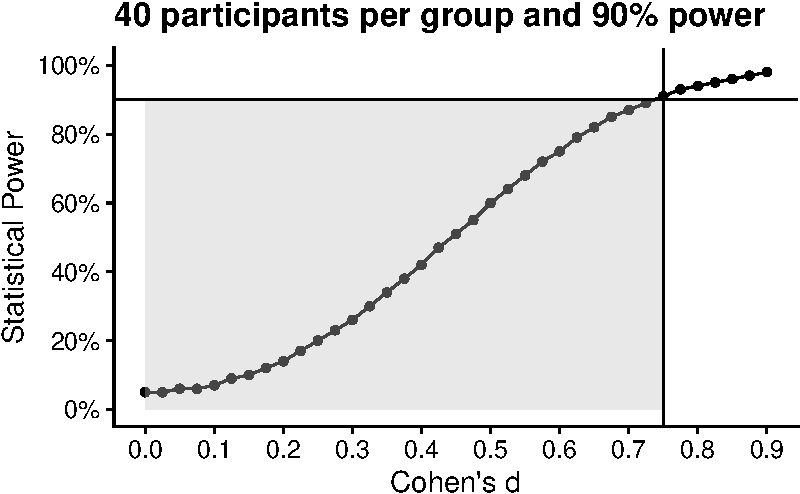
\includegraphics[width=1\textwidth,height=\textheight]{10-power_files/figure-pdf/fig-power-curve-40-1.pdf}

}

\caption{\label{fig-power-curve-40}Power curve for 40 participants per
group and 90\% power.}

\end{figure}%

On the other hand, Figure~\ref{fig-power-curve-80} shows statistical
power against Cohen's d as the effect size for a fixed sample of 80
participants per group. This time, we would have 90\% power to detect
effects of d = 0.53 and there is a smaller grey region. We would have
more power to detect effects larger than d = 0.53 but less power to
detect effects smaller than 0.53.

\begin{figure}

\centering{

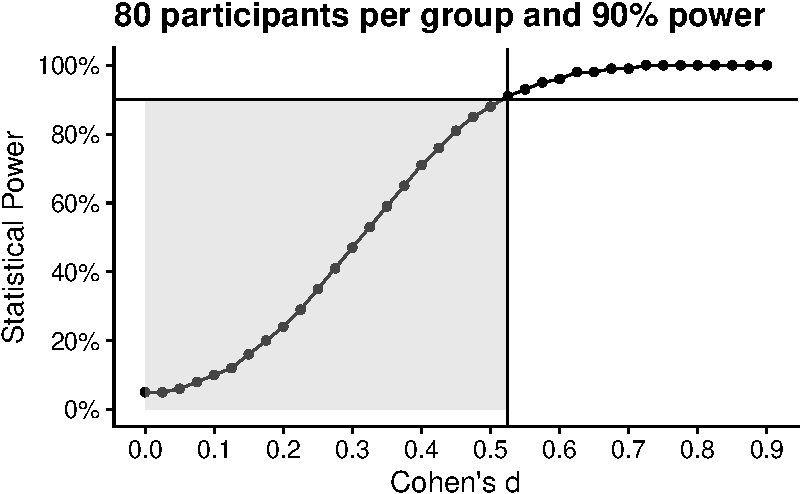
\includegraphics[width=1\textwidth,height=\textheight]{10-power_files/figure-pdf/fig-power-curve-80-1.pdf}

}

\caption{\label{fig-power-curve-80}Power curve for 80 participants per
group and 90\% power.}

\end{figure}%

Hopefully, these demonstrations reinforce the idea of sensitivity and
how power exists along a curve once you have a fixed sample size.

\subsection{Power for regression with a categorical
predictor}\label{power-for-regression-with-a-categorical-predictor}

In Chapters 8 and 9, we recommended expressing your designs as linear
regression models. They have many benefits, but one downside is the
effect size and process we need for power analysis is not the most
intuitive. Typically, people report effect sizes like Cohen's d when
comparing groups, but here we need Cohen's \(f^2\). You can convert
between effect sizes and we recommend the website
\href{https://www.psychometrica.de/effect_size.html\#interpretation}{psychometrica.de}
which has an online calculator for converting effect sizes in section
14. Alternatively, you can use the following code to save \(f^2\) as an
object.

\begin{Shaded}
\begin{Highlighting}[]
\CommentTok{\# enter your Cohen\textquotesingle{}s d value}
\NormalTok{d }\OtherTok{\textless{}{-}} \FloatTok{0.54}

\CommentTok{\# This calculates f2 from d}
\NormalTok{f2 }\OtherTok{\textless{}{-}}\NormalTok{ (d }\SpecialCharTok{/} \DecValTok{2}\NormalTok{)}\SpecialCharTok{\^{}}\DecValTok{2}
\end{Highlighting}
\end{Shaded}

Now we have \(f^2\), we can use the function \texttt{pwr.f2.test()}
which calculates power for regression models. For the equivalent of a
t-test, we have the following new arguments:

\begin{itemize}
\item
  \texttt{u}: The numerator degrees of freedom, the number of predictors
  in your model.
\item
  \texttt{v}: The denominator degrees of freedom, a little more awkward
  but the sample size minus u minus 1.
\item
  \texttt{f2}: The effect size \(f^2\), which is a kind of transformed
  version of \(R^2\) for the amount of variance explained by the model.
\end{itemize}

For our power analysis, we will save the inputs as objects to make it
easier to reuse them, and enter them in the following arguments:

\begin{Shaded}
\begin{Highlighting}[]
\CommentTok{\# number of predictors}
\NormalTok{u }\OtherTok{\textless{}{-}} \DecValTok{1}

\CommentTok{\# alpha for type I error rate}
\NormalTok{alpha }\OtherTok{\textless{}{-}}\NormalTok{ .}\DecValTok{05}

\CommentTok{\# power for 1{-}beta}
\NormalTok{power }\OtherTok{\textless{}{-}}\NormalTok{  .}\DecValTok{90}

\FunctionTok{pwr.f2.test}\NormalTok{(}\AttributeTok{u =}\NormalTok{ u, }
            \AttributeTok{v =} \ConstantTok{NULL}\NormalTok{, }
            \AttributeTok{sig.level =}\NormalTok{ alpha, }
            \AttributeTok{power =}\NormalTok{ power, }
            \AttributeTok{f2 =}\NormalTok{ f2)}
\end{Highlighting}
\end{Shaded}

\begin{verbatim}

     Multiple regression power calculation 

              u = 1
              v = 144.0824
             f2 = 0.0729
      sig.level = 0.05
          power = 0.9
\end{verbatim}

Using the objects from the power analysis, we can calculate the sample
size we need with a little reorganising.

\begin{Shaded}
\begin{Highlighting}[]
\NormalTok{irving\_v }\OtherTok{\textless{}{-}} \FunctionTok{pwr.f2.test}\NormalTok{(}\AttributeTok{u =} \DecValTok{1}\NormalTok{, }
                        \AttributeTok{v =} \ConstantTok{NULL}\NormalTok{, }
                        \AttributeTok{sig.level =}\NormalTok{ .}\DecValTok{05}\NormalTok{, }
                        \AttributeTok{power =}\NormalTok{ .}\DecValTok{90}\NormalTok{, }
                        \AttributeTok{f2 =}\NormalTok{ f2) }\SpecialCharTok{\%\textgreater{}\%} 
  \FunctionTok{pluck}\NormalTok{(}\StringTok{"v"}\NormalTok{) }

\FunctionTok{ceiling}\NormalTok{(irving\_v }\SpecialCharTok{+}\NormalTok{ u }\SpecialCharTok{+} \DecValTok{1}\NormalTok{)}
\end{Highlighting}
\end{Shaded}

\begin{verbatim}
[1] 147
\end{verbatim}

In the t-test power analysis function, we needed 148 participants in
total, so this is off by 1 participant. There are a few steps for
rounding errors here, so this is close enough to show it is the
equivalent but more awkward process.

If you wanted to use this function for a sensitivity power analysis, you
can convert \(f^2\) back to Cohen's d using
\href{https://www.psychometrica.de/effect_size.html\#interpretation}{psychometrica.de}
or use the following code:

\begin{Shaded}
\begin{Highlighting}[]
\CommentTok{\# f2 from the output}
\NormalTok{f2 }\OtherTok{\textless{}{-}}\NormalTok{ .}\DecValTok{073}

\CommentTok{\# convert to d by square root of f2 times 2}
\NormalTok{d }\OtherTok{\textless{}{-}} \FunctionTok{sqrt}\NormalTok{(f2) }\SpecialCharTok{*} \DecValTok{2}
\end{Highlighting}
\end{Shaded}

\section{Power analysis for correlations / continuous
predictors}\label{power-analysis-for-correlations-continuous-predictors}

\subsection{Introduction to the
study}\label{introduction-to-the-study-1}

For this section, we need a new study to work with for a correlation /
continuous predictor. Wingen et al. (2020) were interested in the
relationship between the replication rate in psychology studies and the
public trust in psychology research. The replication crisis has led to a
lot of introspection in the field to consider how we conduct robust
research. However, being honest about the state of the field might be
good for science, but perhaps it is related to lower public trust in
science. We will focus on study 1 which asked the question: does trust
in psychology correlate with expected replicability?

Wingen et al. (2020) reported a power analysis and they aimed for 95\%
power, 5\% alpha, and their smallest effect size of interest was
\emph{r} = .20. Like Irving et al.~(2022), they chose this value based
on a meta-analysis which summarised hundreds of studies across social
psychology. We will use these values as a starting point and adapt them
to see it's impact on the sample size we need.

\subsection{A priori power analysis}\label{a-priori-power-analysis-1}

For Pearson's \emph{r} correlation, there is the function
\texttt{pwr.r.test()}. All the arguments are the same as for the t-test,
apart from we specify \emph{r} as an effect size instead of Cohen's d
and we do not need to specify the type of test.

\begin{Shaded}
\begin{Highlighting}[]
\FunctionTok{pwr.r.test}\NormalTok{(}\AttributeTok{n =} \ConstantTok{NULL}\NormalTok{, }
           \AttributeTok{r =}\NormalTok{ .}\DecValTok{20}\NormalTok{, }
           \AttributeTok{sig.level =}\NormalTok{ .}\DecValTok{05}\NormalTok{, }
           \AttributeTok{power =}\NormalTok{ .}\DecValTok{95}\NormalTok{, }
           \AttributeTok{alternative =} \StringTok{"two.sided"}\NormalTok{)}
\end{Highlighting}
\end{Shaded}

\begin{verbatim}

     approximate correlation power calculation (arctangh transformation) 

              n = 318.2637
              r = 0.2
      sig.level = 0.05
          power = 0.95
    alternative = two.sided
\end{verbatim}

As before, we can isolate the sample size we would need for a study
sensitive to these inputs.

\begin{Shaded}
\begin{Highlighting}[]
\FunctionTok{pwr.r.test}\NormalTok{(}\AttributeTok{n =} \ConstantTok{NULL}\NormalTok{, }
           \AttributeTok{r =}\NormalTok{ .}\DecValTok{20}\NormalTok{, }
           \AttributeTok{sig.level =}\NormalTok{ .}\DecValTok{05}\NormalTok{, }
           \AttributeTok{power =}\NormalTok{ .}\DecValTok{95}\NormalTok{, }
           \AttributeTok{alternative =} \StringTok{"two.sided"}\NormalTok{) }\SpecialCharTok{\%\textgreater{}\%} 
  \FunctionTok{pluck}\NormalTok{(}\StringTok{"n"}\NormalTok{) }\SpecialCharTok{\%\textgreater{}\%} 
  \FunctionTok{ceiling}\NormalTok{()}
\end{Highlighting}
\end{Shaded}

\begin{verbatim}
[1] 319
\end{verbatim}

Our starting point is 319 participants to detect our smallest effect
size of interest \emph{r} = .20 with 95\% power and 5\% alpha.

\begin{tcolorbox}[enhanced jigsaw, breakable, colframe=quarto-callout-tip-color-frame, arc=.35mm, opacitybacktitle=0.6, titlerule=0mm, colbacktitle=quarto-callout-tip-color!10!white, colback=white, toprule=.15mm, bottomtitle=1mm, toptitle=1mm, title=\textcolor{quarto-callout-tip-color}{\faLightbulb}\hspace{0.5em}{Try this}, bottomrule=.15mm, rightrule=.15mm, leftrule=.75mm, coltitle=black, left=2mm, opacityback=0]

With decision making in mind, we can tweak the arguments to see how it
affects the sample size we need. We will tweak one argument at a time,
so your starting point will be the arguments we started with above.

\begin{enumerate}
\def\labelenumi{\arabic{enumi}.}
\item
  If we used a one-tailed test predicting a positive relationship, we
  would need \_\_\_ participants. This reproduces the power analysis
  from Wingen et al., as they used a one-tailed test.
\item
  If we wanted to make fewer type I errors and reduce alpha to .005, we
  would need \_\_\_ participants.
\item
  If we were happy with a larger beta and reduce power to .80 (80\%), we
  would need \_\_\_ participants.
\end{enumerate}

\end{tcolorbox}

\begin{tcolorbox}[enhanced jigsaw, breakable, colframe=quarto-callout-caution-color-frame, arc=.35mm, opacitybacktitle=0.6, titlerule=0mm, colbacktitle=quarto-callout-caution-color!10!white, colback=white, toprule=.15mm, bottomtitle=1mm, toptitle=1mm, title=\textcolor{quarto-callout-caution-color}{\faFire}\hspace{0.5em}{Show me the solution}, bottomrule=.15mm, rightrule=.15mm, leftrule=.75mm, coltitle=black, left=2mm, opacityback=0]

\begin{enumerate}
\def\labelenumi{\arabic{enumi}.}
\tightlist
\item
  We can calculate sample size for a one-tailed test by entering
  \texttt{alternative\ =\ "greater"} or \texttt{alternative\ =\ "less"}.
  This must match the effect size direction or you will receive an
  error.
\end{enumerate}

\begin{Shaded}
\begin{Highlighting}[]
\FunctionTok{pwr.r.test}\NormalTok{(}\AttributeTok{n =} \ConstantTok{NULL}\NormalTok{, }
           \AttributeTok{r =}\NormalTok{ .}\DecValTok{20}\NormalTok{, }
           \AttributeTok{sig.level =}\NormalTok{ .}\DecValTok{05}\NormalTok{, }
           \AttributeTok{power =}\NormalTok{ .}\DecValTok{95}\NormalTok{, }
           \AttributeTok{alternative =} \StringTok{"greater"}\NormalTok{) }\SpecialCharTok{\%\textgreater{}\%} 
  \FunctionTok{pluck}\NormalTok{(}\StringTok{"n"}\NormalTok{) }\SpecialCharTok{\%\textgreater{}\%} 
  \FunctionTok{ceiling}\NormalTok{()}
\end{Highlighting}
\end{Shaded}

\begin{verbatim}
[1] 266
\end{verbatim}

\begin{enumerate}
\def\labelenumi{\arabic{enumi}.}
\setcounter{enumi}{1}
\tightlist
\item
  We can decrease alpha by entering \texttt{alpha\ =\ .005} to calculate
  the sample size for reducing the type I error rate.
\end{enumerate}

\begin{Shaded}
\begin{Highlighting}[]
\FunctionTok{pwr.r.test}\NormalTok{(}\AttributeTok{n =} \ConstantTok{NULL}\NormalTok{, }
           \AttributeTok{r =}\NormalTok{ .}\DecValTok{20}\NormalTok{, }
           \AttributeTok{sig.level =}\NormalTok{ .}\DecValTok{005}\NormalTok{, }
           \AttributeTok{power =}\NormalTok{ .}\DecValTok{95}\NormalTok{, }
           \AttributeTok{alternative =} \StringTok{"two.sided"}\NormalTok{) }\SpecialCharTok{\%\textgreater{}\%} 
  \FunctionTok{pluck}\NormalTok{(}\StringTok{"n"}\NormalTok{) }\SpecialCharTok{\%\textgreater{}\%} 
  \FunctionTok{ceiling}\NormalTok{()}
\end{Highlighting}
\end{Shaded}

\begin{verbatim}
[1] 485
\end{verbatim}

\begin{enumerate}
\def\labelenumi{\arabic{enumi}.}
\setcounter{enumi}{2}
\tightlist
\item
  We can decrease power if we were happy with a larger beta / type II
  error rate by entering \texttt{power\ =\ .80}.
\end{enumerate}

\begin{Shaded}
\begin{Highlighting}[]
\FunctionTok{pwr.r.test}\NormalTok{(}\AttributeTok{n =} \ConstantTok{NULL}\NormalTok{, }
           \AttributeTok{r =}\NormalTok{ .}\DecValTok{20}\NormalTok{, }
           \AttributeTok{sig.level =}\NormalTok{ .}\DecValTok{05}\NormalTok{, }
           \AttributeTok{power =}\NormalTok{ .}\DecValTok{80}\NormalTok{, }
           \AttributeTok{alternative =} \StringTok{"two.sided"}\NormalTok{) }\SpecialCharTok{\%\textgreater{}\%} 
  \FunctionTok{pluck}\NormalTok{(}\StringTok{"n"}\NormalTok{) }\SpecialCharTok{\%\textgreater{}\%} 
  \FunctionTok{ceiling}\NormalTok{()}
\end{Highlighting}
\end{Shaded}

\begin{verbatim}
[1] 194
\end{verbatim}

\end{tcolorbox}

Like for the independent samples t-test, the design phase allows you to
carefully consider the inputs you choose and tweak them depending on how
sensitive you want your study given the resources available to you.
Holding everything else constant, we can summarise the patterns here as:

\begin{itemize}
\item
  Using a one-tailed test
\item
  \begin{enumerate}
  \def\labelenumi{(\Alph{enumi})}
  \tightlist
  \item
    increases\\
  \end{enumerate}
\item
  \begin{enumerate}
  \def\labelenumi{(\Alph{enumi})}
  \setcounter{enumi}{1}
  \tightlist
  \item
    decreases
  \end{enumerate}
\end{itemize}

the sample size you need.

\begin{itemize}
\item
  Reducing alpha
\item
  \begin{enumerate}
  \def\labelenumi{(\Alph{enumi})}
  \tightlist
  \item
    increases\\
  \end{enumerate}
\item
  \begin{enumerate}
  \def\labelenumi{(\Alph{enumi})}
  \setcounter{enumi}{1}
  \tightlist
  \item
    decreases
  \end{enumerate}
\end{itemize}

the sample size you need.

\begin{itemize}
\item
  Reducing power / increasing beta
\item
  \begin{enumerate}
  \def\labelenumi{(\Alph{enumi})}
  \tightlist
  \item
    increases\\
  \end{enumerate}
\item
  \begin{enumerate}
  \def\labelenumi{(\Alph{enumi})}
  \setcounter{enumi}{1}
  \tightlist
  \item
    decreases
  \end{enumerate}
\end{itemize}

the sample size you need.

\subsection{Sensitivity power
analysis}\label{sensitivity-power-analysis-1}

Wingen et al. (2020) is a great example of a sensitivity power analysis
in the wild as they are relatively rare to see in published research.
They explain they recruited participants online, so they ended up with
more participants than they aimed for.

\begin{tcolorbox}[enhanced jigsaw, breakable, colframe=quarto-callout-tip-color-frame, arc=.35mm, opacitybacktitle=0.6, titlerule=0mm, colbacktitle=quarto-callout-tip-color!10!white, colback=white, toprule=.15mm, bottomtitle=1mm, toptitle=1mm, title=\textcolor{quarto-callout-tip-color}{\faLightbulb}\hspace{0.5em}{Try this}, bottomrule=.15mm, rightrule=.15mm, leftrule=.75mm, coltitle=black, left=2mm, opacityback=0]

Their final sample size was \textbf{271}, so try and adapt the function
to calculate the effect size \emph{r} they were sensitive to. Both of
these answers assume 5\% alpha and a one-sided test.

To 2 decimal places, they could detect an effect of \emph{r} = \_\_\_\_
with 80\% power and \emph{r} = \_\_\_ with 95\% power.

\end{tcolorbox}

\begin{tcolorbox}[enhanced jigsaw, breakable, colframe=quarto-callout-caution-color-frame, arc=.35mm, opacitybacktitle=0.6, titlerule=0mm, colbacktitle=quarto-callout-caution-color!10!white, colback=white, toprule=.15mm, bottomtitle=1mm, toptitle=1mm, title=\textcolor{quarto-callout-caution-color}{\faFire}\hspace{0.5em}{Show me the solution}, bottomrule=.15mm, rightrule=.15mm, leftrule=.75mm, coltitle=black, left=2mm, opacityback=0]

You should have had this in a code chunk for 80\% power:

\begin{Shaded}
\begin{Highlighting}[]
\FunctionTok{pwr.r.test}\NormalTok{(}\AttributeTok{n =} \DecValTok{271}\NormalTok{, }
           \AttributeTok{r =} \ConstantTok{NULL}\NormalTok{, }
           \AttributeTok{sig.level =}\NormalTok{ .}\DecValTok{05}\NormalTok{, }
           \AttributeTok{power =}\NormalTok{ .}\DecValTok{80}\NormalTok{, }
           \AttributeTok{alternative =} \StringTok{"greater"}\NormalTok{) }\SpecialCharTok{\%\textgreater{}\%} 
  \FunctionTok{pluck}\NormalTok{(}\StringTok{"r"}\NormalTok{) }\SpecialCharTok{\%\textgreater{}\%} 
  \FunctionTok{round}\NormalTok{(}\AttributeTok{digits =} \DecValTok{2}\NormalTok{)}
\end{Highlighting}
\end{Shaded}

\begin{verbatim}
[1] 0.15
\end{verbatim}

And this in a code chunk for 95\% power:

\begin{Shaded}
\begin{Highlighting}[]
\FunctionTok{pwr.r.test}\NormalTok{(}\AttributeTok{n =} \DecValTok{271}\NormalTok{, }
           \AttributeTok{r =} \ConstantTok{NULL}\NormalTok{, }
           \AttributeTok{sig.level =}\NormalTok{ .}\DecValTok{05}\NormalTok{, }
           \AttributeTok{power =}\NormalTok{ .}\DecValTok{95}\NormalTok{, }
           \AttributeTok{alternative =} \StringTok{"greater"}\NormalTok{) }\SpecialCharTok{\%\textgreater{}\%} 
  \FunctionTok{pluck}\NormalTok{(}\StringTok{"r"}\NormalTok{) }\SpecialCharTok{\%\textgreater{}\%} 
  \FunctionTok{round}\NormalTok{(}\AttributeTok{digits =} \DecValTok{2}\NormalTok{)}
\end{Highlighting}
\end{Shaded}

\begin{verbatim}
[1] 0.2
\end{verbatim}

\end{tcolorbox}

\subsection{Power for regression with a continuous
predictor}\label{power-for-regression-with-a-continuous-predictor}

Like the categorical predictor, we have a mismatch between the effect
size you typically see reported (Pearson's \emph{r}) and the effect size
we need for a regression power analysis (\(f^2\)). The website
\href{https://www.psychometrica.de/effect_size.html\#interpretation}{psychometrica.de}
still works for converting effect sizes in section 14. Alternatively,
you can use the following code to save \(f^2\) as an object.

\begin{Shaded}
\begin{Highlighting}[]
\CommentTok{\# effect size as Pearson\textquotesingle{}s r}
\NormalTok{r }\OtherTok{\textless{}{-}}\NormalTok{ .}\DecValTok{20}

\CommentTok{\# convert to f2 by squaring r values}
\NormalTok{f2 }\OtherTok{\textless{}{-}}\NormalTok{ r}\SpecialCharTok{\^{}}\DecValTok{2} \SpecialCharTok{/}\NormalTok{ (}\DecValTok{1} \SpecialCharTok{{-}}\NormalTok{ r}\SpecialCharTok{\^{}}\DecValTok{2}\NormalTok{)}
\end{Highlighting}
\end{Shaded}

Now we have \(f^2\), we can use the function \texttt{pwr.f2.test()}
which calculates power for regression models.

\begin{Shaded}
\begin{Highlighting}[]
\CommentTok{\# number of predictors}
\NormalTok{u }\OtherTok{\textless{}{-}} \DecValTok{1}

\CommentTok{\# alpha for type I error rate}
\NormalTok{alpha }\OtherTok{\textless{}{-}}\NormalTok{ .}\DecValTok{05}

\CommentTok{\# power for 1{-}beta}
\NormalTok{power }\OtherTok{\textless{}{-}}\NormalTok{  .}\DecValTok{95}

\FunctionTok{pwr.f2.test}\NormalTok{(}\AttributeTok{u =}\NormalTok{ u, }
            \AttributeTok{v =} \ConstantTok{NULL}\NormalTok{, }
            \AttributeTok{sig.level =}\NormalTok{ alpha, }
            \AttributeTok{power =}\NormalTok{ power, }
            \AttributeTok{f2 =}\NormalTok{ f2)}
\end{Highlighting}
\end{Shaded}

\begin{verbatim}

     Multiple regression power calculation 

              u = 1
              v = 311.807
             f2 = 0.04166667
      sig.level = 0.05
          power = 0.95
\end{verbatim}

Using the objects from the power analysis, we can calculate the sample
size we need with a little reorganising.

\begin{Shaded}
\begin{Highlighting}[]
\NormalTok{wingen\_v }\OtherTok{\textless{}{-}} \FunctionTok{pwr.f2.test}\NormalTok{(}\AttributeTok{u =} \DecValTok{1}\NormalTok{, }
                        \AttributeTok{v =} \ConstantTok{NULL}\NormalTok{, }
                        \AttributeTok{sig.level =}\NormalTok{ .}\DecValTok{05}\NormalTok{, }
                        \AttributeTok{power =}\NormalTok{ .}\DecValTok{95}\NormalTok{, }
                        \AttributeTok{f2 =}\NormalTok{ f2) }\SpecialCharTok{\%\textgreater{}\%} 
  \FunctionTok{pluck}\NormalTok{(}\StringTok{"v"}\NormalTok{) }

\FunctionTok{ceiling}\NormalTok{(wingen\_v }\SpecialCharTok{+}\NormalTok{ u }\SpecialCharTok{+} \DecValTok{1}\NormalTok{)}
\end{Highlighting}
\end{Shaded}

\begin{verbatim}
[1] 314
\end{verbatim}

In the Pearson's \emph{r} power analysis function, we needed 319
participants in total, so the estimate is off by 5 participants this
time. We still have a few steps for rounding error, so this is close
enough to show it is the equivalent but more awkward process.

If you wanted to use this function for a sensitivity power analysis, you
can convert \(f^2\) back to Pearson's \(r\) using
\href{https://www.psychometrica.de/effect_size.html\#interpretation}{psychometrica.de}
or use the following code:

\begin{Shaded}
\begin{Highlighting}[]
\CommentTok{\# f2 from the output}
\NormalTok{f2 }\OtherTok{\textless{}{-}}\NormalTok{ .}\DecValTok{042}

\CommentTok{\# convert to r from the square root of f2 / f2 + 1}
\NormalTok{r }\OtherTok{\textless{}{-}} \FunctionTok{sqrt}\NormalTok{(f2 }\SpecialCharTok{/}\NormalTok{ (f2 }\SpecialCharTok{+} \DecValTok{1}\NormalTok{))}
\end{Highlighting}
\end{Shaded}

\section{Reporting a power analysis}\label{reporting-a-power-analysis}

Bakker et al. (2020) warned that only 20\% of power analyses contained
enough information to be fully reproducible. To report your power
analysis, the reader needs the following four key pieces of information:

\begin{itemize}
\item
  The type of test you based the power analysis on (e.g., t-test,
  correlation, regression),
\item
  The software used to calculate power (i.e., cite the pwr package, see
  \hyperref[citing-r-rstudio]{How to cite R}),
\item
  The inputs that you used (alpha, power, effect size, sample size,
  tails), and
\item
  Why you chose those inputs.
\end{itemize}

In this chapter, we will only cover the first three. The justification
for your inputs comes under evaluation skills, so we will work on that
in the course materials. Please note there is no single `correct' way to
report a power analysis, we just provide examples. Just be sure that you
have the four key pieces of information.

\subsection{Reporting a t-test power
analysis}\label{reporting-a-t-test-power-analysis}

For a t-test, the key distinctive input is Cohen's d as the effect size.

\begin{quote}
``To detect an effect size of Cohen's d = 0.54 with 90\% power (alpha =
.05, two-tailed), the pwr package (Champely, 2020) in R (R Core Team,
2024) suggests we would need 74 participants per group (N = 148) for an
independent samples t-test.''
\end{quote}

Alternatively, if you reported a sensitivity power analysis, the
emphasis goes to the effect size your study would be sensitive to.

\begin{quote}
``With our final sample size of 40 participants per group, a sensitivity
power analysis for an independent samples t-test using the pwr package
(Champely, 2020; R Core Team, 2024) showed we could detect an effect
size of d = 0.73 with 90\% power (5\% alpha, two-sided).''
\end{quote}

\subsection{Reporting a correlation power
analysis}\label{reporting-a-correlation-power-analysis}

For a correlation, the key distinctive input is Pearson's \emph{r} as
the effect size.

\begin{quote}
``To detect an effect size of \emph{r} = .20 with 95\% power (alpha =
.05, one-tailed), the pwr package (Champely, 2020) in R (R Core Team,
2024) suggests we would need 266 participants for a Pearson's \emph{r}
correlation.''
\end{quote}

And for a sensitivity power analysis.

\begin{quote}
``With our final sample size of 271 participants, a sensitivity power
analysis for a Pearson's \emph{r} correlation using the pwr package
(Champely, 2020; R Core Team, 2024) showed we could detect an effect
size of \emph{r} = .20 with 95\% power (5\% alpha, one-sided).''
\end{quote}

\subsection{Reporting a regression power
analysis}\label{reporting-a-regression-power-analysis}

For regression, the key distinctive inputs are \(f^2\) as the effect
size, including any details of converting effect sizes, plus the number
of predictors.

\begin{quote}
``To detect an effect size of Cohen's \(f^2\) = .073, we first converted
the effect size from d = 0.54. For 90\% power (alpha = .05, two-tailed),
the pwr package (Champely, 2020) in R (R Core Team, 2024) suggests we
would need 147 participants split into two groups for a regression model
with one categorical predictor.''
\end{quote}

For a sensitivity power analysis, remember to include a note of any
effect size conversions.

\begin{quote}
``We used the pwr package (Champely, 2020; R Core Team, 2024) to conduct
a sensitivity power analysis for linear regression with one predictor.
With a final sample size of 319, we would be able to detect an effect
size of Cohen's \(f^2\) = .041 (95\% power, 5\% alpha). Converted to
Pearson's \emph{r}, this would be an effect size of \emph{r} = .20.''
\end{quote}

\section{Test Yourself}\label{test-yourself-7}

To end the chapter, we have some knowledge check questions to test your
understanding of the concepts we covered in the chapter. We then have
some error mode tasks to see if you can find the solution to some common
errors in the concepts we covered in this chapter.

\subsection{Knowledge check}\label{knowledge-check-9}

\textbf{Question 1}. If you want to conduct an \emph{a priori} power
analysis , what input do you leave blank to solve for?

\begin{itemize}
\tightlist
\item
  \begin{enumerate}
  \def\labelenumi{(\Alph{enumi})}
  \tightlist
  \item
    effect size\\
  \end{enumerate}
\item
  \begin{enumerate}
  \def\labelenumi{(\Alph{enumi})}
  \setcounter{enumi}{1}
  \tightlist
  \item
    power\\
  \end{enumerate}
\item
  \begin{enumerate}
  \def\labelenumi{(\Alph{enumi})}
  \setcounter{enumi}{2}
  \tightlist
  \item
    sample size\\
  \end{enumerate}
\item
  \begin{enumerate}
  \def\labelenumi{(\Alph{enumi})}
  \setcounter{enumi}{3}
  \tightlist
  \item
    alpha
  \end{enumerate}
\end{itemize}

\textbf{Question 2}. If you want to conduct a sensitivity power analysis
, what input do you leave blank to solve for?

\begin{itemize}
\tightlist
\item
  \begin{enumerate}
  \def\labelenumi{(\Alph{enumi})}
  \tightlist
  \item
    effect size\\
  \end{enumerate}
\item
  \begin{enumerate}
  \def\labelenumi{(\Alph{enumi})}
  \setcounter{enumi}{1}
  \tightlist
  \item
    alpha\\
  \end{enumerate}
\item
  \begin{enumerate}
  \def\labelenumi{(\Alph{enumi})}
  \setcounter{enumi}{2}
  \tightlist
  \item
    power\\
  \end{enumerate}
\item
  \begin{enumerate}
  \def\labelenumi{(\Alph{enumi})}
  \setcounter{enumi}{3}
  \tightlist
  \item
    sample size
  \end{enumerate}
\end{itemize}

Read the following output for an \emph{a priori} power analysis. The
next two questions are based on this output.

\begin{verbatim}

     Two-sample t test power calculation 

              n = 89.95986
              d = 0.42
      sig.level = 0.05
          power = 0.8
    alternative = two.sided

NOTE: n is number in *each* group
\end{verbatim}

\textbf{Question 3}. Our smallest effect size of interest is:

\begin{itemize}
\tightlist
\item
  \begin{enumerate}
  \def\labelenumi{(\Alph{enumi})}
  \tightlist
  \item
    d = 0.80\\
  \end{enumerate}
\item
  \begin{enumerate}
  \def\labelenumi{(\Alph{enumi})}
  \setcounter{enumi}{1}
  \tightlist
  \item
    d = 0.42\\
  \end{enumerate}
\item
  \begin{enumerate}
  \def\labelenumi{(\Alph{enumi})}
  \setcounter{enumi}{2}
  \tightlist
  \item
    r = .42\\
  \end{enumerate}
\item
  \begin{enumerate}
  \def\labelenumi{(\Alph{enumi})}
  \setcounter{enumi}{3}
  \tightlist
  \item
    r = .80
  \end{enumerate}
\end{itemize}

\textbf{Question 4}. For these inputs, we would need to recruit how many
participants per group?

\begin{itemize}
\tightlist
\item
  \begin{enumerate}
  \def\labelenumi{(\Alph{enumi})}
  \tightlist
  \item
    42\\
  \end{enumerate}
\item
  \begin{enumerate}
  \def\labelenumi{(\Alph{enumi})}
  \setcounter{enumi}{1}
  \tightlist
  \item
    80\\
  \end{enumerate}
\item
  \begin{enumerate}
  \def\labelenumi{(\Alph{enumi})}
  \setcounter{enumi}{2}
  \tightlist
  \item
    89\\
  \end{enumerate}
\item
  \begin{enumerate}
  \def\labelenumi{(\Alph{enumi})}
  \setcounter{enumi}{3}
  \tightlist
  \item
    90
  \end{enumerate}
\end{itemize}

Read the following output for a sensitivity power analysis. The next two
questions are based on this output.

\begin{verbatim}

     approximate correlation power calculation (arctangh transformation) 

              n = 72
              r = 0.3695127
      sig.level = 0.05
          power = 0.9
    alternative = two.sided
\end{verbatim}

\textbf{Question 5}. Our final sample size was:

\begin{itemize}
\tightlist
\item
  \begin{enumerate}
  \def\labelenumi{(\Alph{enumi})}
  \tightlist
  \item
    90\\
  \end{enumerate}
\item
  \begin{enumerate}
  \def\labelenumi{(\Alph{enumi})}
  \setcounter{enumi}{1}
  \tightlist
  \item
    50\\
  \end{enumerate}
\item
  \begin{enumerate}
  \def\labelenumi{(\Alph{enumi})}
  \setcounter{enumi}{2}
  \tightlist
  \item
    36\\
  \end{enumerate}
\item
  \begin{enumerate}
  \def\labelenumi{(\Alph{enumi})}
  \setcounter{enumi}{3}
  \tightlist
  \item
    72
  \end{enumerate}
\end{itemize}

\textbf{Question 6}. For these inputs, what effect size would we be
sensitive to detect?

\begin{itemize}
\tightlist
\item
  \begin{enumerate}
  \def\labelenumi{(\Alph{enumi})}
  \tightlist
  \item
    r = .37\\
  \end{enumerate}
\item
  \begin{enumerate}
  \def\labelenumi{(\Alph{enumi})}
  \setcounter{enumi}{1}
  \tightlist
  \item
    r = .90\\
  \end{enumerate}
\item
  \begin{enumerate}
  \def\labelenumi{(\Alph{enumi})}
  \setcounter{enumi}{2}
  \tightlist
  \item
    r = .72\\
  \end{enumerate}
\item
  \begin{enumerate}
  \def\labelenumi{(\Alph{enumi})}
  \setcounter{enumi}{3}
  \tightlist
  \item
    r = .05
  \end{enumerate}
\end{itemize}

\subsection{Error mode}\label{error-mode-20}

The following questions are designed to introduce you to making and
fixing errors. For this topic, we focus on simple linear regression
between two continuous variables. There are not many outright errors
that people make here, more misspecifications that are not doing what
you think they are doing.

Create and save a new R Markdown file for these activities. Delete the
example code, so your file is blank from line 10. Create a new code
chunk to load the packages tidyverse and pwr.

Below, we have several variations of a code chunk error or
misspecification. Copy and paste them into your R Markdown file below
the code chunk to load tidyverse and pwr. Once you have copied the
activities, click knit and look at the error message you receive. See if
you can fix the error and get it working before checking the answer.

\begin{itemize}
\tightlist
\item
  unconverted effect sizes
\end{itemize}

\textbf{Question 7}. Copy the following code chunk into your R Markdown
file and press knit. You should get a cryptic sounding error like
\texttt{Error\ in\ uniroot(function(n)\ eval(p.body)\ -\ power,\ c(4\ +\ 1e-10,\ 1e+09)):\ f()\ values\ at\ end\ points\ not\ of\ opposite\ sign}.

\begin{Shaded}
\begin{Highlighting}[]
\InformationTok{\textasciigrave{}\textasciigrave{}\textasciigrave{}\{r\}}
\InformationTok{pwr.r.test(n = NULL, }
\InformationTok{           r = .20, }
\InformationTok{           sig.level = .05, }
\InformationTok{           power = .95, }
\InformationTok{           alternative = "less")}
\InformationTok{\textasciigrave{}\textasciigrave{}\textasciigrave{}}
\end{Highlighting}
\end{Shaded}

\begin{tcolorbox}[enhanced jigsaw, breakable, colframe=quarto-callout-caution-color-frame, arc=.35mm, opacitybacktitle=0.6, titlerule=0mm, colbacktitle=quarto-callout-caution-color!10!white, colback=white, toprule=.15mm, bottomtitle=1mm, toptitle=1mm, title=\textcolor{quarto-callout-caution-color}{\faFire}\hspace{0.5em}{Explain the solution}, bottomrule=.15mm, rightrule=.15mm, leftrule=.75mm, coltitle=black, left=2mm, opacityback=0]

In this example, we specified a positive effect size but negative
one-tailed test. They must be consistent, so you either need to make the
hypothesis the same:

\begin{Shaded}
\begin{Highlighting}[]
\FunctionTok{pwr.r.test}\NormalTok{(}\AttributeTok{n =} \ConstantTok{NULL}\NormalTok{, }
           \AttributeTok{r =}\NormalTok{ .}\DecValTok{20}\NormalTok{, }
           \AttributeTok{sig.level =}\NormalTok{ .}\DecValTok{05}\NormalTok{, }
           \AttributeTok{power =}\NormalTok{ .}\DecValTok{95}\NormalTok{, }
           \AttributeTok{alternative =} \StringTok{"greater"}\NormalTok{)}
\end{Highlighting}
\end{Shaded}

Or the effect size the same:

\begin{Shaded}
\begin{Highlighting}[]
\FunctionTok{pwr.r.test}\NormalTok{(}\AttributeTok{n =} \ConstantTok{NULL}\NormalTok{, }
           \AttributeTok{r =} \SpecialCharTok{{-}}\NormalTok{.}\DecValTok{20}\NormalTok{, }
           \AttributeTok{sig.level =}\NormalTok{ .}\DecValTok{05}\NormalTok{, }
           \AttributeTok{power =}\NormalTok{ .}\DecValTok{95}\NormalTok{, }
           \AttributeTok{alternative =} \StringTok{"less"}\NormalTok{)}
\end{Highlighting}
\end{Shaded}

Both will produce the same sample size as it is the absolute effect
which is important, but we recommend making it consistent with your
research question / hypothesis.

\end{tcolorbox}

\textbf{Question 8}. Copy the following code chunk into your R Markdown
file and press knit. You want to conduct a sensitivity power analysis
when you have unequal sample sizes. You should get the following error:
\texttt{Error\ in\ pwr.t.test(n1\ =\ 40,\ n2\ =\ 50,\ d\ =\ NULL,\ sig.level\ =\ 0.05,\ power\ =\ 0.9,\ \ :\ unused\ arguments\ (n1\ =\ 40,\ n2\ =\ 50)}.

\begin{Shaded}
\begin{Highlighting}[]
\InformationTok{\textasciigrave{}\textasciigrave{}\textasciigrave{}\{r\}}
\InformationTok{pwr.t.test(n1 = 40, }
\InformationTok{           n2 = 50,}
\InformationTok{           d = NULL, }
\InformationTok{           sig.level = .05, }
\InformationTok{           power = .90, }
\InformationTok{           alternative = "two.sided")}
\InformationTok{\textasciigrave{}\textasciigrave{}\textasciigrave{}}
\end{Highlighting}
\end{Shaded}

\begin{tcolorbox}[enhanced jigsaw, breakable, colframe=quarto-callout-caution-color-frame, arc=.35mm, opacitybacktitle=0.6, titlerule=0mm, colbacktitle=quarto-callout-caution-color!10!white, colback=white, toprule=.15mm, bottomtitle=1mm, toptitle=1mm, title=\textcolor{quarto-callout-caution-color}{\faFire}\hspace{0.5em}{Explain the solution}, bottomrule=.15mm, rightrule=.15mm, leftrule=.75mm, coltitle=black, left=2mm, opacityback=0]

In this example, we used the wrong function. \texttt{pwr.t.test()} only
accepts \texttt{n} as a single argument. If you want a sensitivity power
analysis for unequal sample sizes, you need the function
\texttt{pwr.t2n.test()}:

\begin{Shaded}
\begin{Highlighting}[]
\FunctionTok{pwr.t2n.test}\NormalTok{(}\AttributeTok{n1 =} \DecValTok{40}\NormalTok{, }\AttributeTok{n2 =} \DecValTok{50}\NormalTok{,}
           \AttributeTok{d =} \ConstantTok{NULL}\NormalTok{, }
           \AttributeTok{sig.level =}\NormalTok{ .}\DecValTok{05}\NormalTok{, }
           \AttributeTok{power =}\NormalTok{ .}\DecValTok{90}\NormalTok{, }
           \AttributeTok{alternative =} \StringTok{"two.sided"}\NormalTok{)}
\end{Highlighting}
\end{Shaded}

\end{tcolorbox}

\textbf{Question 9}. Copy the following code chunk into your R Markdown
file and press knit. In your research to establish your smallest effect
size of interest, you found a meta-analysis which found the average
effect size for your topic was d = 0.54. For your correlational study,
you use this effect size for your \emph{a priori} power analysis.
This\ldots works, but is this all consistent?

\begin{Shaded}
\begin{Highlighting}[]
\InformationTok{\textasciigrave{}\textasciigrave{}\textasciigrave{}\{r\}}
\InformationTok{pwr.r.test(n = NULL, }
\InformationTok{           r = .54, }
\InformationTok{           sig.level = .05, }
\InformationTok{           power = .95, }
\InformationTok{           alternative = "two.sided")}
\InformationTok{\textasciigrave{}\textasciigrave{}\textasciigrave{}}
\end{Highlighting}
\end{Shaded}

\begin{tcolorbox}[enhanced jigsaw, breakable, colframe=quarto-callout-caution-color-frame, arc=.35mm, opacitybacktitle=0.6, titlerule=0mm, colbacktitle=quarto-callout-caution-color!10!white, colback=white, toprule=.15mm, bottomtitle=1mm, toptitle=1mm, title=\textcolor{quarto-callout-caution-color}{\faFire}\hspace{0.5em}{Explain the solution}, bottomrule=.15mm, rightrule=.15mm, leftrule=.75mm, coltitle=black, left=2mm, opacityback=0]

In this example, we used the wrong effect size. We see this error a lot
when people are looking for past studies to inform their smallest effect
size of interest. You find a meta-analysis which is perfect, but it
reports Cohen's d when you want Pearson's \emph{r} for your study. You
can convert between effect sizes (with the caveat the studies should be
comparable), but the same number means different things. Mistaking d =
0.54 for Pearson's \emph{r} is going to vastly underestimate the sample
size you need, as it would be converted to \emph{r} = .26.

\begin{Shaded}
\begin{Highlighting}[]
\FunctionTok{pwr.r.test}\NormalTok{(}\AttributeTok{n =} \ConstantTok{NULL}\NormalTok{, }
           \AttributeTok{r =}\NormalTok{ .}\DecValTok{26}\NormalTok{, }
           \AttributeTok{sig.level =}\NormalTok{ .}\DecValTok{05}\NormalTok{, }
           \AttributeTok{power =}\NormalTok{ .}\DecValTok{95}\NormalTok{, }
           \AttributeTok{alternative =} \StringTok{"two.sided"}\NormalTok{)}
\end{Highlighting}
\end{Shaded}

\end{tcolorbox}

\section{Words from this Chapter}\label{words-from-this-chapter-9}

Below you will find a list of words that were used in this chapter that
might be new to you in case it helps to have somewhere to refer back to
what they mean. The links in this table take you to the entry for the
words in the \href{https://psyteachr.github.io/glossary/}{PsyTeachR
Glossary}. Note that the Glossary is written by numerous members of the
team and as such may use slightly different terminology from that shown
in the chapter.

\begin{longtable}[]{@{}
  >{\raggedright\arraybackslash}p{(\columnwidth - 2\tabcolsep) * \real{0.2279}}
  >{\raggedright\arraybackslash}p{(\columnwidth - 2\tabcolsep) * \real{0.7721}}@{}}
\toprule\noalign{}
\begin{minipage}[b]{\linewidth}\raggedright
term
\end{minipage} & \begin{minipage}[b]{\linewidth}\raggedright
definition
\end{minipage} \\
\midrule\noalign{}
\endhead
\bottomrule\noalign{}
\endlastfoot
\href{https://psyteachr.github.io/glossary/a\#alpha}{alpha} & (stats)
The cutoff value for making a decision to reject the null hypothesis;
(graphics) A value between 0 and 1 used to control the levels of
transparency in a plot \\
\href{https://psyteachr.github.io/glossary/b\#beta}{beta} & The false
negative rate we accept for a statistical test. \\
\href{https://psyteachr.github.io/glossary/f\#false-negative}{false-negative}
& When a test concludes there is no effect when there really is an
effect \\
\href{https://psyteachr.github.io/glossary/f\#false-positive}{false-positive}
& When a test concludes there is an effect when there really is no
effect \\
\href{https://psyteachr.github.io/glossary/h\#hypothesis}{hypothesis} &
A proposed explanation made on the basis of limited evidence as a
starting point for further investigation. \\
\href{https://psyteachr.github.io/glossary/p\#power}{power} & The
probability of rejecting the null hypothesis when it is false. \\
\href{https://psyteachr.github.io/glossary/p\#probability}{probability}
& A number between 0 and 1 where 0 indicates impossibility of the event
and 1 indicates certainty \\
\end{longtable}

\section{End of Chapter}\label{end-of-chapter-9}

Great work, being able to conduct a power analysis is a great skill to
have for designing an informative study. Although things have improved
over the years, it is still relatively rare to see a study in the wild
report a power analysis to justify their sample size. Keep in mind they
involve a lot of subjective decision making as the values you choose for
alpha, power, and your smallest effect size have flexibility. A larger
sample - and hence more powerful study - would always be useful, but you
are never working with unlimited resources. You must make compromises
and think about whether you can conduct an informative study with the
resources available to you. This means the hard work comes into making
decisions about the values you enter, rather than the data skills for
power analysis being difficult.

In the next - and final for the Research Methods 1 component - chapter,
we cover screening data and decision making in data analysis. In
Chapters 8 and 9, we covered topics like diagnostic checks for
statistical models. Some of them looked fine, whereas some looked
potentially problematic. In the next chapter, we work through the
decisions you must make when analysing data like checking for missing
data, outliers, and issues with diagnostic checks. Importantly, we
outline the kind of solutions you can consider for those problems which
we omitted in previous chapters.

\bookmarksetup{startatroot}

\chapter{Missing data, outliers, and checking
assumptions}\label{missing-data-outliers-and-checking-assumptions}

In this chapter, you will work on decisions that come up in data
analysis. In Chapters 8 and 9, you learnt about different inferential
statistics and checking assumptions, but not what your options are once
you experience different problems. In this final chapter for the
Research Methods 1 content, you will learn about identifying and
excluding missing data, different strategies for identifying and
excluding extreme values or outliers, and your options when checking
modelling assumptions.

\textbf{Chapter Intended Learning Outcomes (ILOs)}

By the end of this chapter, you will be able to:

\begin{itemize}
\item
  Identify missing data and justify your strategy for excluding missing
  data.
\item
  Identify extreme values or outliers and justify your strategy for
  handling them.
\item
  Justify your choice of statistical test or modelling approach given
  assumption checks.
\end{itemize}

\section{Chapter preparation}\label{chapter-preparation-8}

\subsection{Organising your files and project for the
chapter}\label{organising-your-files-and-project-for-the-chapter-8}

For this chapter, we are going to revisit the data sets you worked with
in Chapters 8 (Dawtry et al., 2015) and 9 (Lopez et al., 2023). They
each presented some useful examples for checking modelling assumptions
and the decisions that go into data analysis. We might not use both data
sets for each topic we cover, but they will be useful to demonstrate
some of the problems and decisions we highlighted in previous chapters,
but did not explore solutions.

Before we can get started, you need to organise your files and project
for the chapter, so your working directory is in order.

\begin{enumerate}
\def\labelenumi{\arabic{enumi}.}
\item
  In your folder for research methods and the book
  \texttt{ResearchMethods1\_2/Quant\_Fundamentals}, create a new folder
  called \texttt{Chapter\_11\_screening\_data}. Within
  \texttt{Chapter\_11\_screening\_data}, create two new folders called
  \texttt{data} and \texttt{figures}.
\item
  Create an R Project for \texttt{Chapter\_11\_screening\_data} as an
  existing directory for your chapter folder. This should now be your
  working directory.
\item
  Create a new R Markdown document and give it a sensible title
  describing the chapter, such as
  \texttt{11\ Missing\ Data,\ Outliers,\ and\ Assumptions}. Delete
  everything below line 10 so you have a blank file to work with and
  save the file in your \texttt{Chapter\_11\_screening\_data} folder.
\item
  The Dawtry et al. (2015) data wrangling steps were quite long, so
  please save this clean version of the data to focus on screening data
  in this chapter:
  \href{data/Dawtry_2015_clean.csv}{Dawtry\_2015\_clean.csv}. You will
  also need to save the data from Lopez et al. (2023) if you have not
  downloaded it yet: \href{data/Lopez_2023.csv}{Lopez\_2023.csv}. Right
  click the link and select ``save link as'', or clicking the link will
  save the files to your Downloads. Make sure that you save the files as
  ``.csv''. Save or copy the files to your \texttt{data/} folder within
  \texttt{Chapter\_11\_screening\_data}.
\end{enumerate}

You are now ready to start working on the chapter!

\subsection{Activity 1 - Read and wrangle the
data}\label{activity-1---read-and-wrangle-the-data-3}

As the first activity, try and test yourself by completing the following
task list to read and wrangle the two data files. There is nothing extra
to do with this version of the Dawtry data and one small step for the
Lopez data.

\begin{tcolorbox}[enhanced jigsaw, breakable, colframe=quarto-callout-tip-color-frame, arc=.35mm, opacitybacktitle=0.6, titlerule=0mm, colbacktitle=quarto-callout-tip-color!10!white, colback=white, toprule=.15mm, bottomtitle=1mm, toptitle=1mm, title=\textcolor{quarto-callout-tip-color}{\faLightbulb}\hspace{0.5em}{Try this}, bottomrule=.15mm, rightrule=.15mm, leftrule=.75mm, coltitle=black, left=2mm, opacityback=0]

To read and wrangle the data, complete the following tasks:

\begin{enumerate}
\def\labelenumi{\arabic{enumi}.}
\item
  Load the following packages:

  \begin{itemize}
  \item
    performance
  \item
    tidyverse
  \end{itemize}
\item
  Read the data file \texttt{data/Dawtry\_2015\_clean.csv} to the object
  name \texttt{dawtry\_clean}.
\item
  Read the data file \texttt{data/Lopez\_2023.csv} to the object name
  \texttt{lopez\_data}.
\item
  Create a new object called \texttt{lopez\_clean} based on
  \texttt{lopez\_data}:

  \begin{itemize}
  \tightlist
  \item
    Create a new variable called \texttt{Condition\_label} by recoding
    \texttt{Condition}. ``0'' is the ``Control'' group and ``1'' is the
    ``Experimental'' group.
  \end{itemize}
\end{enumerate}

\end{tcolorbox}

\begin{tcolorbox}[enhanced jigsaw, breakable, colframe=quarto-callout-caution-color-frame, arc=.35mm, opacitybacktitle=0.6, titlerule=0mm, colbacktitle=quarto-callout-caution-color!10!white, colback=white, toprule=.15mm, bottomtitle=1mm, toptitle=1mm, title=\textcolor{quarto-callout-caution-color}{\faFire}\hspace{0.5em}{Show me the solution}, bottomrule=.15mm, rightrule=.15mm, leftrule=.75mm, coltitle=black, left=2mm, opacityback=0]

You should have the following in a code chunk:

\begin{Shaded}
\begin{Highlighting}[]
\CommentTok{\# load the relevant packages}
\FunctionTok{library}\NormalTok{(performance)}
\FunctionTok{library}\NormalTok{(tidyverse)}

\CommentTok{\# Read the Dawtry\_2015\_clean.csv file }
\NormalTok{dawtry\_clean }\OtherTok{\textless{}{-}} \FunctionTok{read\_csv}\NormalTok{(}\StringTok{"data/Dawtry\_2015\_clean.csv"}\NormalTok{)}

\CommentTok{\# Read the Lopez\_2023.csv file }
\NormalTok{lopez\_data }\OtherTok{\textless{}{-}} \FunctionTok{read\_csv}\NormalTok{(}\StringTok{"data/Lopez\_2023.csv"}\NormalTok{)}

\CommentTok{\# recode condition}
\NormalTok{lopez\_clean }\OtherTok{\textless{}{-}}\NormalTok{ lopez\_data }\SpecialCharTok{\%\textgreater{}\%} 
  \FunctionTok{mutate}\NormalTok{(}\AttributeTok{Condition\_label =} \FunctionTok{case\_match}\NormalTok{(Condition,}
                                      \DecValTok{0} \SpecialCharTok{\textasciitilde{}} \StringTok{"Control"}\NormalTok{,}
                                      \DecValTok{1} \SpecialCharTok{\textasciitilde{}} \StringTok{"Experimental"}\NormalTok{))}
\end{Highlighting}
\end{Shaded}

\end{tcolorbox}

\section{Missing data}\label{missing-data}

Checking whether data are missing are relatively straight forward.
\textbf{Missing values} in a spreadsheet will be recorded as NA and
there are a few ways of identifying them. The much more difficult part
of missing data is considering \emph{why} they are missing in the first
place. For example, it might be because:

\begin{itemize}
\item
  Your participants accidentally missed a question.
\item
  You made a mistake while setting up your questionnaire/experiment and
  some responses did not save.
\item
  Your participants intentionally did not want to answer a question.
\item
  Your participants did not turn up to a final testing session.
\end{itemize}

For the first two reasons, it is not ideal as we are losing data but
there is no systematic pattern to why the data is missing. For the
latter two reasons, there might be a relationship between a key variable
and whether the data are missing. This is where it is particularly
important to consider the role of missing data. We are focusing on data
skills here rather than the conceptual understanding, but missing data
are commonly categorised as:

\begin{itemize}
\item
  \textbf{Missing completely at random}.
\item
  \textbf{Missing at random}.
\item
  \textbf{Missing not at random}.
\end{itemize}

For this introductory course, we do not have time to investigate
strategies to address missing data apart from focusing on complete cases
and ignoring missing data, but you might find Jakobsen et al. (2017)
useful if you want to explore options like data imputation.

\subsection{Activity 2 - Identifying missing
data}\label{activity-2---identifying-missing-data}

Returning to data skills, the simplest way of getting an overview of
whether any data are missing is using the \texttt{summary()} function.
For this part, we will focus on \texttt{dawtry\_clean} from Dawtry et
al. (2015).

\begin{Shaded}
\begin{Highlighting}[]
\FunctionTok{summary}\NormalTok{(dawtry\_clean)}
\end{Highlighting}
\end{Shaded}

\begin{verbatim}
       PS      Household_Income Political_Preference      age      
 Min.   :  1   Min.   :    20   Min.   :1.000        Min.   :19.0  
 1st Qu.: 77   1st Qu.: 25000   1st Qu.:3.000        1st Qu.:28.0  
 Median :153   Median : 42000   Median :4.000        Median :33.5  
 Mean   :153   Mean   : 54732   Mean   :4.465        Mean   :37.4  
 3rd Qu.:229   3rd Qu.: 75000   3rd Qu.:6.000        3rd Qu.:46.0  
 Max.   :305   Max.   :350000   Max.   :9.000        Max.   :69.0  
               NA's   :4        NA's   :4            NA's   :1     
     gender     Population_Inequality_Gini_Index Population_Mean_Income
 Min.   :1.00   Min.   :14.26                    Min.   : 14205        
 1st Qu.:1.00   1st Qu.:31.10                    1st Qu.: 47250        
 Median :1.00   Median :35.66                    Median : 58650        
 Mean   :1.48   Mean   :35.51                    Mean   : 58605        
 3rd Qu.:2.00   3rd Qu.:40.73                    3rd Qu.: 67875        
 Max.   :2.00   Max.   :57.45                    Max.   :138645        
 NA's   :3                                                             
 Social_Circle_Inequality_Gini_Index Social_Circle_Mean_Income
 Min.   : 2.00                       Min.   : 12000           
 1st Qu.:19.79                       1st Qu.: 36000           
 Median :25.59                       Median : 51060           
 Mean   :26.35                       Mean   : 54294           
 3rd Qu.:33.27                       3rd Qu.: 66375           
 Max.   :61.36                       Max.   :148500           
                                                              
 fairness_satisfaction redistribution
 Min.   :1.000         Min.   :1.00  
 1st Qu.:2.000         1st Qu.:3.25  
 Median :3.000         Median :4.00  
 Mean   :3.539         Mean   :3.91  
 3rd Qu.:5.000         3rd Qu.:4.75  
 Max.   :9.000         Max.   :6.00  
                                     
\end{verbatim}

We get a range of summary statistics for each variable but importantly
for our purposes here, the final entry is
\texttt{NA\textquotesingle{}s}, where relevant. We can see there are 4
missing values for household income, 4 for political preference, 1 for
age, and 3 for gender.

\begin{tcolorbox}[enhanced jigsaw, breakable, colframe=quarto-callout-tip-color-frame, arc=.35mm, opacitybacktitle=0.6, titlerule=0mm, colbacktitle=quarto-callout-tip-color!10!white, colback=white, toprule=.15mm, bottomtitle=1mm, toptitle=1mm, title=\textcolor{quarto-callout-tip-color}{\faLightbulb}\hspace{0.5em}{Try this}, bottomrule=.15mm, rightrule=.15mm, leftrule=.75mm, coltitle=black, left=2mm, opacityback=0]

If you explore \texttt{lopez\_clean} from Lopez et al. (2023), do we
have any missing data to worry about?

\begin{itemize}
\tightlist
\item
  \begin{enumerate}
  \def\labelenumi{(\Alph{enumi})}
  \tightlist
  \item
    Yes\\
  \end{enumerate}
\item
  \begin{enumerate}
  \def\labelenumi{(\Alph{enumi})}
  \setcounter{enumi}{1}
  \tightlist
  \item
    No
  \end{enumerate}
\end{itemize}

\end{tcolorbox}

\begin{tcolorbox}[enhanced jigsaw, breakable, colframe=quarto-callout-caution-color-frame, arc=.35mm, opacitybacktitle=0.6, titlerule=0mm, colbacktitle=quarto-callout-caution-color!10!white, colback=white, toprule=.15mm, bottomtitle=1mm, toptitle=1mm, title=\textcolor{quarto-callout-caution-color}{\faFire}\hspace{0.5em}{Solution}, bottomrule=.15mm, rightrule=.15mm, leftrule=.75mm, coltitle=black, left=2mm, opacityback=0]

Yes, it looks like there is also a small amount of missing data here.
There is 1 for sex, 2 for estimated ounces, and 3 for estimates
calories.

\begin{Shaded}
\begin{Highlighting}[]
\FunctionTok{summary}\NormalTok{(lopez\_clean)}
\end{Highlighting}
\end{Shaded}

\begin{verbatim}
 ParticipantID       Sex              Age          Ethnicity    
 Min.   :1001   Min.   :0.0000   Min.   :18.00   Min.   :1.000  
 1st Qu.:1202   1st Qu.:1.0000   1st Qu.:19.00   1st Qu.:3.000  
 Median :1462   Median :1.0000   Median :20.00   Median :3.000  
 Mean   :1456   Mean   :0.8099   Mean   :20.47   Mean   :3.261  
 3rd Qu.:1704   3rd Qu.:1.0000   3rd Qu.:21.00   3rd Qu.:4.000  
 Max.   :1928   Max.   :3.0000   Max.   :54.00   Max.   :8.000  
                NA's   :1                                       
   OzEstimate       CalEstimate      M_postsoup     F_CaloriesConsumed
 Min.   :  0.010   Min.   :  1.0   Min.   : 0.600   Min.   :  13.31   
 1st Qu.:  2.000   1st Qu.: 50.0   1st Qu.: 5.575   1st Qu.: 123.65   
 Median :  4.000   Median : 90.0   Median : 8.700   Median : 192.97   
 Mean   :  6.252   Mean   :124.6   Mean   :10.203   Mean   : 226.30   
 3rd Qu.:  8.000   3rd Qu.:160.0   3rd Qu.:13.125   3rd Qu.: 291.11   
 Max.   :100.000   Max.   :800.0   Max.   :46.200   Max.   :1024.72   
 NA's   :2         NA's   :3                                          
   Condition      Condition_label   
 Min.   :0.0000   Length:464        
 1st Qu.:0.0000   Class :character  
 Median :0.0000   Mode  :character  
 Mean   :0.4698                     
 3rd Qu.:1.0000                     
 Max.   :1.0000                     
                                    
\end{verbatim}

\end{tcolorbox}

\subsection{Activity 3 - Removing missing
data}\label{activity-3---removing-missing-data}

Once we know whether missing data are present, we must consider what to
do with them. For this chapter, we are only going to control removing
participants, but you could apply a data imputation technique at this
point if appropriate.

For all the modelling techniques we apply in this book, the functions
will remove participants who have one or more missing values from any
variable involved in the analysis. The functions will give you a warning
to highlight when this happens, but it is normally a good idea to remove
participants with missing data yourself so you have a note of how many
participants you remove.

For \texttt{dawtry\_clean}, the tidyverse function \texttt{drop\_na()}
is the easiest way of removing missing data, either participants with
any missing data or by specifying individual variables.

\begin{Shaded}
\begin{Highlighting}[]
\NormalTok{dawtry\_all\_missing }\OtherTok{\textless{}{-}}\NormalTok{ dawtry\_clean }\SpecialCharTok{\%\textgreater{}\%} 
  \FunctionTok{drop\_na}\NormalTok{()}

\NormalTok{dawtry\_income\_missing }\OtherTok{\textless{}{-}}\NormalTok{ dawtry\_clean }\SpecialCharTok{\%\textgreater{}\%} 
  \FunctionTok{drop\_na}\NormalTok{(Household\_Income)}
\end{Highlighting}
\end{Shaded}

We can compare the number of participants by using the \texttt{nrow()}
function to count how many rows are in each object.

\begin{Shaded}
\begin{Highlighting}[]
\CommentTok{\# How many rows in the full data? }
\FunctionTok{nrow}\NormalTok{(dawtry\_clean)}

\CommentTok{\# How many rows when we remove missing data in one variable? }
\FunctionTok{nrow}\NormalTok{(dawtry\_income\_missing)}

\CommentTok{\# How many rows when we remove any missing value?}
\FunctionTok{nrow}\NormalTok{(dawtry\_all\_missing)}
\end{Highlighting}
\end{Shaded}

\begin{verbatim}
[1] 305
[1] 301
[1] 294
\end{verbatim}

Like most data skills and statistics concepts, the key skill here comes
in decision making; documenting and justifying the approach that you
take.

\section{Outliers}\label{outliers}

The next data screening concept revolves around identifying potential
outliers. Like missing data, the difficulty here comes in first deciding
what an outlier is and then deciding on what to do with it. Leys et al.
(2019) mention one study found 14 definitions and 39 unique ways of
identifying outliers, so this is our second key area of decision making.
Leys et al.~categorise outliers into three types:

\begin{enumerate}
\def\labelenumi{\arabic{enumi}.}
\item
  \textbf{Error outliers}.
\item
  \textbf{Interesting outliers}.
\item
  \textbf{Random outliers}.
\end{enumerate}

Even simpler, we can consider values as legitimate or not legitimate.
Error outliers would be not legitimate as they represent a mistake or
error, so they would potentially provide misleading results. These are
values you can justify removing or correcting as they should not be
there in the first place.

Interesting and random outliers would be legitimate as they are not
clear mistakes or errors; they are just different to the majority of
values in the data. In most cases, it is not a good idea to remove these
kind of values as they potentially tell you something interesting, but
you might need to approach the data analysis in a different way to
ensure the results are robust to extreme values.

\subsection{Activity 4- Identifying error
outliers}\label{activity-4--identifying-error-outliers}

Unless you can specifically identify values or participants you know
contain errors, the main way to check is by ensuring the values are
within known limits.

We can look at \texttt{dawtry\_clean} and the key variables we explored
in Chapter 8. Fairness and satisfaction was on a 1-9 scale, so we can
check the minimum and maximum values and create a plot. For example, we
can isolate the variable and apply the \texttt{summary()} function.

\begin{Shaded}
\begin{Highlighting}[]
\NormalTok{dawtry\_clean }\SpecialCharTok{\%\textgreater{}\%} 
  \FunctionTok{select}\NormalTok{(fairness\_satisfaction) }\SpecialCharTok{\%\textgreater{}\%} 
  \FunctionTok{summary}\NormalTok{()}
\end{Highlighting}
\end{Shaded}

\begin{verbatim}
 fairness_satisfaction
 Min.   :1.000        
 1st Qu.:2.000        
 Median :3.000        
 Mean   :3.539        
 3rd Qu.:5.000        
 Max.   :9.000        
\end{verbatim}

The minimum and maximum values are nice and consistent with what we
expect.

For a visual check, we can also plot the minimum and maximum possible
values on a boxplot. This is just a check for you, so you do not need to
worry so much about the presentation.

\begin{Shaded}
\begin{Highlighting}[]
\NormalTok{dawtry\_clean }\SpecialCharTok{\%\textgreater{}\%} 
  \FunctionTok{ggplot}\NormalTok{(}\FunctionTok{aes}\NormalTok{(}\AttributeTok{y =}\NormalTok{ fairness\_satisfaction, }\AttributeTok{x =} \StringTok{""}\NormalTok{)) }\SpecialCharTok{+} \CommentTok{\# make x blank }
  \FunctionTok{geom\_boxplot}\NormalTok{() }\SpecialCharTok{+} 
  \FunctionTok{scale\_y\_continuous}\NormalTok{(}\AttributeTok{limits =} \FunctionTok{c}\NormalTok{(}\DecValTok{1}\NormalTok{, }\DecValTok{9}\NormalTok{), }
                     \AttributeTok{breaks =} \FunctionTok{seq}\NormalTok{(}\DecValTok{1}\NormalTok{, }\DecValTok{9}\NormalTok{, }\DecValTok{1}\NormalTok{)) }\SpecialCharTok{+} 
  \FunctionTok{geom\_hline}\NormalTok{(}\AttributeTok{yintercept =} \FunctionTok{c}\NormalTok{(}\DecValTok{1}\NormalTok{, }\DecValTok{9}\NormalTok{), }\CommentTok{\# min and max values}
             \AttributeTok{linetype =} \DecValTok{2}\NormalTok{) }\CommentTok{\# create dashed line}
\end{Highlighting}
\end{Shaded}

\begin{center}
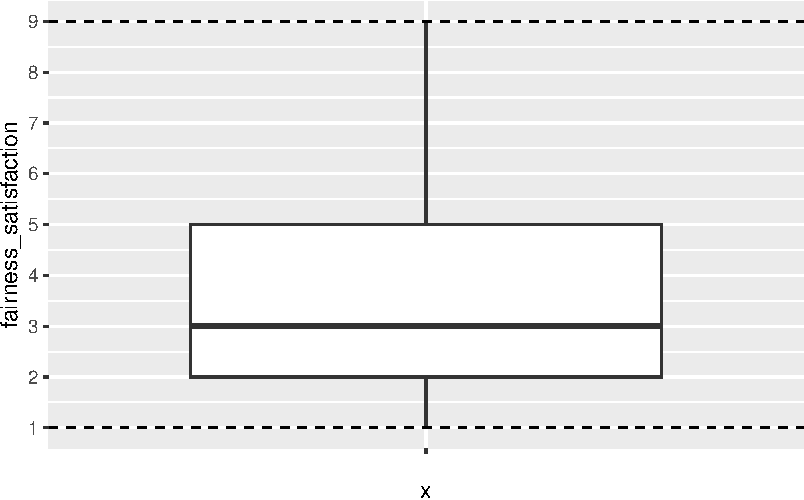
\includegraphics[width=1\textwidth,height=\textheight]{11-screening-data_files/figure-pdf/unnamed-chunk-7-1.pdf}
\end{center}

\begin{tcolorbox}[enhanced jigsaw, breakable, colframe=quarto-callout-tip-color-frame, arc=.35mm, opacitybacktitle=0.6, titlerule=0mm, colbacktitle=quarto-callout-tip-color!10!white, colback=white, toprule=.15mm, bottomtitle=1mm, toptitle=1mm, title=\textcolor{quarto-callout-tip-color}{\faLightbulb}\hspace{0.5em}{Try this}, bottomrule=.15mm, rightrule=.15mm, leftrule=.75mm, coltitle=black, left=2mm, opacityback=0]

If you explore \texttt{redistribution} from \texttt{dawtry\_clean}, the
minimum and maximum values are 1-6. Does it look like there are any
problematic looking values?

\begin{itemize}
\tightlist
\item
  \begin{enumerate}
  \def\labelenumi{(\Alph{enumi})}
  \tightlist
  \item
    Yes\\
  \end{enumerate}
\item
  \begin{enumerate}
  \def\labelenumi{(\Alph{enumi})}
  \setcounter{enumi}{1}
  \tightlist
  \item
    No
  \end{enumerate}
\end{itemize}

\end{tcolorbox}

\begin{tcolorbox}[enhanced jigsaw, breakable, colframe=quarto-callout-caution-color-frame, arc=.35mm, opacitybacktitle=0.6, titlerule=0mm, colbacktitle=quarto-callout-caution-color!10!white, colback=white, toprule=.15mm, bottomtitle=1mm, toptitle=1mm, title=\textcolor{quarto-callout-caution-color}{\faFire}\hspace{0.5em}{Solution}, bottomrule=.15mm, rightrule=.15mm, leftrule=.75mm, coltitle=black, left=2mm, opacityback=0]

No, it looks like all values are within the expected 1-6 range.

\begin{Shaded}
\begin{Highlighting}[]
\NormalTok{dawtry\_clean }\SpecialCharTok{\%\textgreater{}\%} 
  \FunctionTok{select}\NormalTok{(redistribution) }\SpecialCharTok{\%\textgreater{}\%} 
  \FunctionTok{summary}\NormalTok{()}
\end{Highlighting}
\end{Shaded}

\begin{verbatim}
 redistribution
 Min.   :1.00  
 1st Qu.:3.25  
 Median :4.00  
 Mean   :3.91  
 3rd Qu.:4.75  
 Max.   :6.00  
\end{verbatim}

We can also confirm this with a visual check.

\begin{Shaded}
\begin{Highlighting}[]
\NormalTok{dawtry\_clean }\SpecialCharTok{\%\textgreater{}\%} 
  \FunctionTok{ggplot}\NormalTok{(}\FunctionTok{aes}\NormalTok{(}\AttributeTok{y =}\NormalTok{ redistribution, }\AttributeTok{x =} \StringTok{""}\NormalTok{)) }\SpecialCharTok{+} \CommentTok{\# make x blank }
  \FunctionTok{geom\_boxplot}\NormalTok{() }\SpecialCharTok{+} 
  \FunctionTok{scale\_y\_continuous}\NormalTok{(}\AttributeTok{limits =} \FunctionTok{c}\NormalTok{(}\DecValTok{1}\NormalTok{, }\DecValTok{6}\NormalTok{), }
                     \AttributeTok{breaks =} \FunctionTok{seq}\NormalTok{(}\DecValTok{1}\NormalTok{, }\DecValTok{6}\NormalTok{, }\DecValTok{1}\NormalTok{)) }\SpecialCharTok{+} 
  \FunctionTok{geom\_hline}\NormalTok{(}\AttributeTok{yintercept =} \FunctionTok{c}\NormalTok{(}\DecValTok{1}\NormalTok{, }\DecValTok{6}\NormalTok{), }\CommentTok{\# min and max values}
             \AttributeTok{linetype =} \DecValTok{2}\NormalTok{) }\CommentTok{\# create dashed line}
\end{Highlighting}
\end{Shaded}

\begin{center}
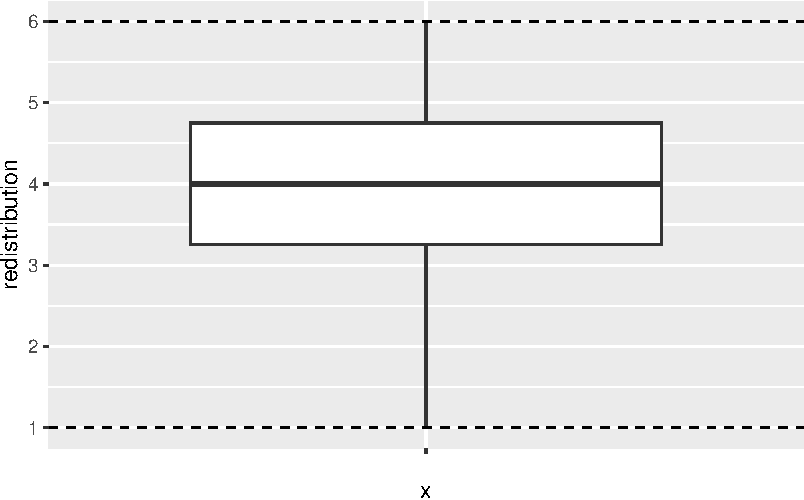
\includegraphics[width=1\textwidth,height=\textheight]{11-screening-data_files/figure-pdf/unnamed-chunk-9-1.pdf}
\end{center}

\end{tcolorbox}

If you did identify error outliers to remove, then you could use
\texttt{filter()} (Chapter 5) to directly remove values outside your
known range, or you could first use \texttt{case\_when()} to code
observations as outliers or not (Chapter 4), before deciding to filter
them out.

\subsection{Activity 5- Identifying interesting or random
outliers}\label{activity-5--identifying-interesting-or-random-outliers}

Identifying error outliers relies on manually setting known minimum and
maximum values, whereas identifying interesting or random outliers
relies on data driven boundaries. For this example, we focus on
univariate outliers, where we focus on one variable at a time. When we
return to checking assumptions of regression models, you can identify
interesting or random outliers through observations with large leverage
/ Cook's distance values.

In general, we recommend not removing outliers providing you are
confident they are not errors. It is better to focus on modelling your
outcome in a more robust way. However, it is also important you know how
to identify errors for strategies you will come across in published
research.

We focus here on setting boundaries using the median absolute deviation
(MAD) as recommended by Leys et al. (2019). You will see other
approaches in the literature, but this method is useful as it's
influenced less by the very outliers it is trying to identify. We will
use \texttt{lopez\_clean} from Lopez et al. (2023) for this section.

There are two main steps to this process because we have two groups and
each group will have different boundaries. If you only have individual
variables, then you could just \texttt{mutate()} your data, without the
initial \texttt{group\_by()} and \texttt{summarise()} step.

First, we group by the condition to get one value per group. We then
calculate a few values for the median ounces of soup, 3 times the MAD in
line with Leys et al., then calculating the upper and lower bound using
these objects.

\begin{Shaded}
\begin{Highlighting}[]
\CommentTok{\# create a new object with values per group}
\NormalTok{mad\_bounds }\OtherTok{\textless{}{-}}\NormalTok{ lopez\_clean }\SpecialCharTok{\%\textgreater{}\%} 
  \FunctionTok{group\_by}\NormalTok{(Condition\_label) }\SpecialCharTok{\%\textgreater{}\%} 
  \FunctionTok{summarise}\NormalTok{(}\AttributeTok{oz\_median =} \FunctionTok{median}\NormalTok{(M\_postsoup), }\CommentTok{\# median of soup in oz}
            \AttributeTok{oz\_MAD =} \DecValTok{3} \SpecialCharTok{*} \FunctionTok{mad}\NormalTok{(M\_postsoup), }\CommentTok{\# 3 times the MAD}
            \AttributeTok{lower =}\NormalTok{ oz\_median }\SpecialCharTok{{-}}\NormalTok{ oz\_MAD, }\CommentTok{\# lower bound }
            \AttributeTok{upper =}\NormalTok{ oz\_median }\SpecialCharTok{+}\NormalTok{ oz\_MAD) }\CommentTok{\# upper bound}

\NormalTok{mad\_bounds}
\end{Highlighting}
\end{Shaded}

\begin{verbatim}
# A tibble: 2 x 5
  Condition_label oz_median oz_MAD lower upper
  <chr>               <dbl>  <dbl> <dbl> <dbl>
1 Control               7.8   14.7 -6.88  22.5
2 Experimental         10.6   17.6 -6.97  28.2
\end{verbatim}

In this example, the lower bound is lower than 0 as the smallest
possible value. The upper bounds are then between 22 and 28 depending on
the group.

Second, we must add these values to the other information we have
available. We join the data sets using \texttt{Condition\_label}. This
adds the relevant values to each group. We then use \texttt{mutate()}
and \texttt{case\_when()} to label values as outliers or not. If they
are outside the lower and upper bounds, they are labelled as
``outlier''. If they are inside the lower and upper bounds, they are
labelled as ``no outlier''.

\begin{Shaded}
\begin{Highlighting}[]
\NormalTok{lopez\_mad }\OtherTok{\textless{}{-}}\NormalTok{ lopez\_clean }\SpecialCharTok{\%\textgreater{}\%} 
  \FunctionTok{inner\_join}\NormalTok{(mad\_bounds, }\AttributeTok{by =} \StringTok{"Condition\_label"}\NormalTok{) }\SpecialCharTok{\%\textgreater{}\%} 
  \FunctionTok{mutate}\NormalTok{(}\AttributeTok{oz\_outlier =} \FunctionTok{case\_when}\NormalTok{(M\_postsoup }\SpecialCharTok{\textless{}}\NormalTok{ lower }\SpecialCharTok{|}\NormalTok{ M\_postsoup }\SpecialCharTok{\textgreater{}}\NormalTok{ upper }\SpecialCharTok{\textasciitilde{}} \StringTok{"Outlier"}\NormalTok{,}
\NormalTok{                                M\_postsoup }\SpecialCharTok{\textgreater{}=}\NormalTok{ lower }\SpecialCharTok{|}\NormalTok{ M\_postsoup }\SpecialCharTok{\textless{}=}\NormalTok{ upper }\SpecialCharTok{\textasciitilde{}} \StringTok{"No Outlier"}\NormalTok{))}
\end{Highlighting}
\end{Shaded}

We can use these in one of two ways. First, we can visualise the
presence of outliers by adding coloured points. These are checks for you
again, so you do not need to worry about the plot formatting.

\begin{Shaded}
\begin{Highlighting}[]
\NormalTok{lopez\_mad }\SpecialCharTok{\%\textgreater{}\%} 
  \FunctionTok{ggplot}\NormalTok{(}\FunctionTok{aes}\NormalTok{(}\AttributeTok{x =}\NormalTok{ Condition\_label, }\AttributeTok{y =}\NormalTok{ M\_postsoup)) }\SpecialCharTok{+} 
  \FunctionTok{geom\_boxplot}\NormalTok{() }\SpecialCharTok{+} 
  \FunctionTok{geom\_point}\NormalTok{(}\FunctionTok{aes}\NormalTok{(}\AttributeTok{colour =}\NormalTok{ oz\_outlier)) }\CommentTok{\# needs to be within aes to set dynamic values}
\end{Highlighting}
\end{Shaded}

\begin{center}
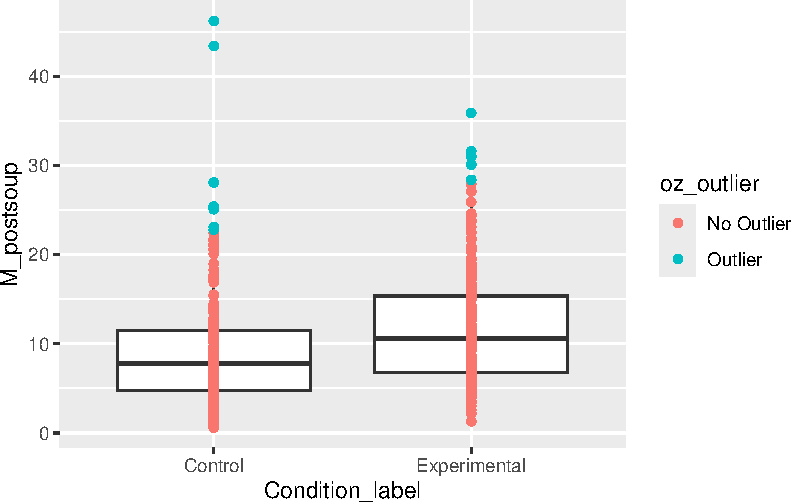
\includegraphics[width=1\textwidth,height=\textheight]{11-screening-data_files/figure-pdf/unnamed-chunk-12-1.pdf}
\end{center}

We can see a few values per group flagged as outliers using this
criterion. If you did decide to remove outliers, then you could use
filter to remove them:

\begin{Shaded}
\begin{Highlighting}[]
\NormalTok{lopez\_remove }\OtherTok{\textless{}{-}}\NormalTok{ lopez\_mad }\SpecialCharTok{\%\textgreater{}\%} 
  \FunctionTok{filter}\NormalTok{(oz\_outlier }\SpecialCharTok{==} \StringTok{"No Outlier"}\NormalTok{)}
\end{Highlighting}
\end{Shaded}

\begin{tcolorbox}[enhanced jigsaw, breakable, colframe=quarto-callout-tip-color-frame, arc=.35mm, opacitybacktitle=0.6, titlerule=0mm, colbacktitle=quarto-callout-tip-color!10!white, colback=white, toprule=.15mm, bottomtitle=1mm, toptitle=1mm, title=\textcolor{quarto-callout-tip-color}{\faLightbulb}\hspace{0.5em}{Try this}, bottomrule=.15mm, rightrule=.15mm, leftrule=.75mm, coltitle=black, left=2mm, opacityback=0]

If you switch to \texttt{dawtry\_clean} from Dawtry et al. (2015), apply
the MAD procedure to the variable \texttt{fairness\_satisfaction}. Does
it look like there are any outliers using this criterion?

\begin{itemize}
\tightlist
\item
  \begin{enumerate}
  \def\labelenumi{(\Alph{enumi})}
  \tightlist
  \item
    Yes\\
  \end{enumerate}
\item
  \begin{enumerate}
  \def\labelenumi{(\Alph{enumi})}
  \setcounter{enumi}{1}
  \tightlist
  \item
    No
  \end{enumerate}
\end{itemize}

.

\end{tcolorbox}

\begin{tcolorbox}[enhanced jigsaw, breakable, colframe=quarto-callout-caution-color-frame, arc=.35mm, opacitybacktitle=0.6, titlerule=0mm, colbacktitle=quarto-callout-caution-color!10!white, colback=white, toprule=.15mm, bottomtitle=1mm, toptitle=1mm, title=\textcolor{quarto-callout-caution-color}{\faFire}\hspace{0.5em}{Solution}, bottomrule=.15mm, rightrule=.15mm, leftrule=.75mm, coltitle=black, left=2mm, opacityback=0]

No, none of the values are outside the MAD thresholds. The thresholds
are well beyond the minimum and maximum possible values of 1-9 for this
variable.

\begin{Shaded}
\begin{Highlighting}[]
\NormalTok{dawtry\_mad }\OtherTok{\textless{}{-}}\NormalTok{ dawtry\_clean }\SpecialCharTok{\%\textgreater{}\%} 
  \FunctionTok{mutate}\NormalTok{(}\AttributeTok{fs\_median =} \FunctionTok{median}\NormalTok{(fairness\_satisfaction), }\CommentTok{\# median of fairness/satisfaction}
         \AttributeTok{fs\_MAD =} \DecValTok{3} \SpecialCharTok{*} \FunctionTok{mad}\NormalTok{(fairness\_satisfaction), }\CommentTok{\# 3 times the MAD}
         \AttributeTok{lower =}\NormalTok{ fs\_median }\SpecialCharTok{{-}}\NormalTok{ fs\_MAD, }\CommentTok{\# lower bound }
         \AttributeTok{upper =}\NormalTok{ fs\_median }\SpecialCharTok{+}\NormalTok{ fs\_MAD,  }\CommentTok{\# upper bound}
         \AttributeTok{fs\_outlier =} \FunctionTok{case\_when}\NormalTok{(fairness\_satisfaction }\SpecialCharTok{\textless{}}\NormalTok{ lower }\SpecialCharTok{|}\NormalTok{ fairness\_satisfaction }\SpecialCharTok{\textgreater{}}\NormalTok{ upper }\SpecialCharTok{\textasciitilde{}} \StringTok{"Outlier"}\NormalTok{,}
\NormalTok{                                fairness\_satisfaction }\SpecialCharTok{\textgreater{}=}\NormalTok{ lower }\SpecialCharTok{|}\NormalTok{ fairness\_satisfaction }\SpecialCharTok{\textless{}=}\NormalTok{ upper }\SpecialCharTok{\textasciitilde{}} \StringTok{"No Outlier"}\NormalTok{))}
\end{Highlighting}
\end{Shaded}

For this variable and it's bounded scale, no value is above or below the
thresholds. You can see this in the data, or add horizontal lines in a
plot since we are only plotting one variable. The dashed lines are the
MAD thresholds and the solid lines are the minimum and maximum possible
values.

\begin{Shaded}
\begin{Highlighting}[]
\NormalTok{dawtry\_mad }\SpecialCharTok{\%\textgreater{}\%} 
  \FunctionTok{ggplot}\NormalTok{(}\FunctionTok{aes}\NormalTok{(}\AttributeTok{y =}\NormalTok{ fairness\_satisfaction, }\AttributeTok{x =} \StringTok{""}\NormalTok{)) }\SpecialCharTok{+} 
  \FunctionTok{geom\_boxplot}\NormalTok{() }\SpecialCharTok{+} 
  \FunctionTok{geom\_hline}\NormalTok{(}\FunctionTok{aes}\NormalTok{(}\AttributeTok{yintercept =}\NormalTok{ lower), }
             \AttributeTok{linetype =} \DecValTok{2}\NormalTok{) }\SpecialCharTok{+} \CommentTok{\# dashed line}
  \FunctionTok{geom\_hline}\NormalTok{(}\AttributeTok{yintercept =} \FunctionTok{c}\NormalTok{(}\DecValTok{1}\NormalTok{, }\DecValTok{9}\NormalTok{)) }\SpecialCharTok{+} 
  \FunctionTok{geom\_hline}\NormalTok{(}\FunctionTok{aes}\NormalTok{(}\AttributeTok{yintercept =}\NormalTok{ upper), }
             \AttributeTok{linetype =} \DecValTok{2}\NormalTok{) }\SpecialCharTok{+} 
  \FunctionTok{scale\_y\_continuous}\NormalTok{(}\AttributeTok{limits =} \FunctionTok{c}\NormalTok{(}\SpecialCharTok{{-}}\DecValTok{4}\NormalTok{, }\DecValTok{10}\NormalTok{), }
                     \AttributeTok{breaks =} \FunctionTok{seq}\NormalTok{(}\SpecialCharTok{{-}}\DecValTok{4}\NormalTok{, }\DecValTok{10}\NormalTok{, }\DecValTok{2}\NormalTok{))}
\end{Highlighting}
\end{Shaded}

\begin{center}
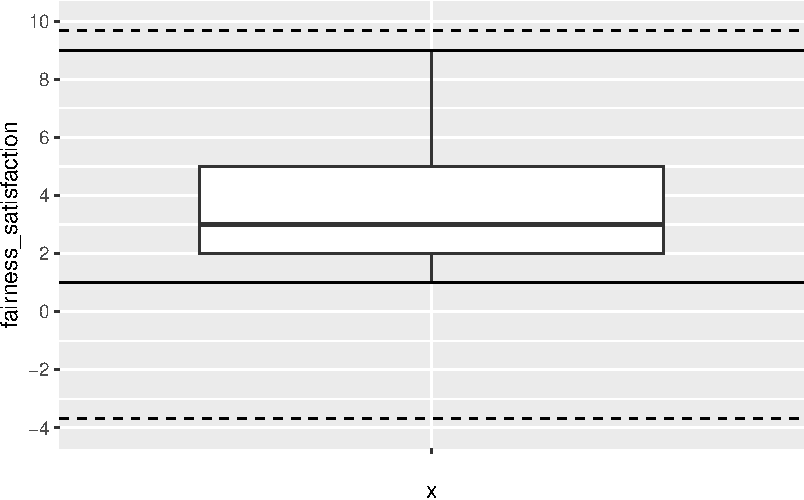
\includegraphics[width=1\textwidth,height=\textheight]{11-screening-data_files/figure-pdf/unnamed-chunk-15-1.pdf}
\end{center}

\end{tcolorbox}

Remember: identifying outliers is a crucial researcher degree of
freedom, so pre-register your choice of outlier detection wherever
possible, and document how many outliers you removed. We still recommend
favouring a more robust model, but you can make an informed decision now
you know how to identify outliers in the data.

\section{Checking assumptions}\label{checking-assumptions-2}

The final section revisits checking assumptions from Chapter 8 and 9. In
those chapters, we introduced the concepts and stuck with the output
regardless of whether we were happy with the assumptions or not. In this
chapter, we will introduce potential solutions.

As a reminder, the assumptions for simple linear regression are:

\begin{enumerate}
\def\labelenumi{\arabic{enumi}.}
\item
  The outcome is interval/ratio level data.
\item
  The predictor variable is interval/ratio or categorical (with two
  levels at a time).
\item
  All values of the outcome variable are independent (i.e., each score
  should come from a different participant/observation).
\item
  The predictors have non-zero variance.
\item
  The relationship between the outcome and predictor is linear.
\item
  The residuals should be normally distributed.
\item
  There should be homoscedasticity.
\end{enumerate}

Assumptions 1-4 are pretty straight forward as they relate to your
understanding of the design or a simple check on the data. On the other
hand, assumptions 5-7 require diagnostic checks.

For this part, we focus on Lopez et al. (2023) as the assumptions did
not look quite right in Chapter 9. As a reminder, we can get a quick
diagnostic check by running \texttt{plot()} on the model object:

\begin{Shaded}
\begin{Highlighting}[]
\CommentTok{\# Condition as a factor containing 0 and 1}
\NormalTok{lm\_cals\_numbers }\OtherTok{\textless{}{-}} \FunctionTok{lm}\NormalTok{(}\AttributeTok{formula =}\NormalTok{ F\_CaloriesConsumed }\SpecialCharTok{\textasciitilde{}}\NormalTok{ Condition, }
                      \AttributeTok{data =}\NormalTok{ lopez\_clean)}

\CommentTok{\# Change the panel layout to 2 x 2}
\FunctionTok{par}\NormalTok{(}\AttributeTok{mfrow =} \FunctionTok{c}\NormalTok{(}\DecValTok{2}\NormalTok{,}\DecValTok{2}\NormalTok{))}

\CommentTok{\# plot the diagnostic plots }
\FunctionTok{plot}\NormalTok{(lm\_cals\_numbers)}
\end{Highlighting}
\end{Shaded}

\begin{center}
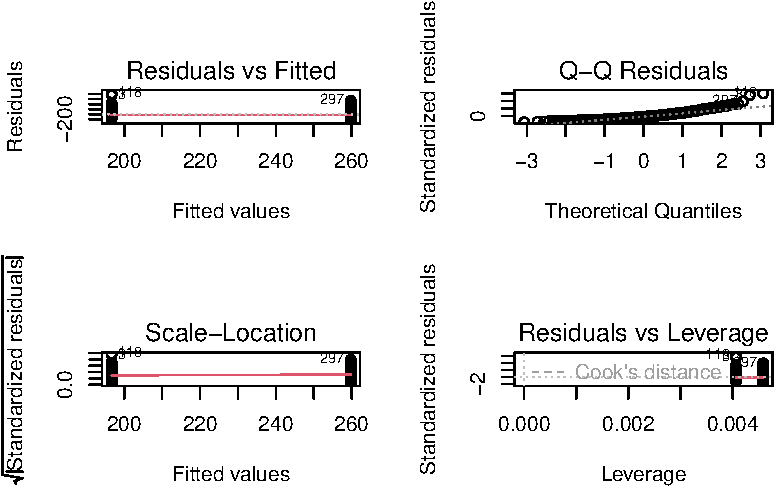
\includegraphics[width=1\textwidth,height=\textheight]{11-screening-data_files/figure-pdf/unnamed-chunk-16-1.pdf}
\end{center}

All of the checks look good apart from normality. We have a clear
deviation from the line to curve around at lower and higher values along
the x-axis. In Chapter 9, we said we would stick with it as it was
consistent with the original article's analyses, but now we will outline
options available to you:

\begin{enumerate}
\def\labelenumi{\arabic{enumi}.}
\item
  Parametric tests are robust.
\item
  Treat the data as non-parametric.
\item
  Use an alternative model.
\end{enumerate}

\subsection{Activity 6 - Parametric tests are
robust}\label{activity-6---parametric-tests-are-robust}

One get out jail free card is doing nothing as the parametric tests are
robust to violations of assumptions. You will often hear this and it is
largely true under certain conditions. Knief \& Forstmeier (2021) report
a simulation study where they explore how violating assumptions like
linearity, normality, and outliers affect the results of parametric
statistical tests like simple linear regression. They found the tests
were robust to violations - particularly normality - apart from when
there were extreme outliers which could bias the results.

In the Lopez et al.~example, we identified a few outliers using the 3
times the MAD criterion and the strictest Cook's distance cut-off in
Chapter 9, but normality was the only notable problem in the diagnostic
checks. One option would be to feel reassured the results are robust to
minor violations and explain that in your report.

The second option would be checking the results are robust to the
presence of outliers. Remember, we advise excluding outliers as a last
resort if you consider them legitimate, but it provides a robustness
check to see if you get similar conclusions with and without the
outliers. For example, we can exclude outliers using the MAD criterion
and check the results:

\begin{Shaded}
\begin{Highlighting}[]
\CommentTok{\# remove outliers under 3 * MAD }

\NormalTok{lm\_cals\_outliers }\OtherTok{\textless{}{-}} \FunctionTok{lm}\NormalTok{(}\AttributeTok{formula =}\NormalTok{ F\_CaloriesConsumed }\SpecialCharTok{\textasciitilde{}}\NormalTok{ Condition, }
                      \AttributeTok{data =} \FunctionTok{filter}\NormalTok{(lopez\_mad, }
\NormalTok{                                    oz\_outlier }\SpecialCharTok{==} \StringTok{"No Outlier"}\NormalTok{))}

\FunctionTok{summary}\NormalTok{(lm\_cals\_outliers)}
\end{Highlighting}
\end{Shaded}

\begin{verbatim}

Call:
lm(formula = F_CaloriesConsumed ~ Condition, data = filter(lopez_mad, 
    oz_outlier == "No Outlier"))

Residuals:
    Min      1Q  Median      3Q     Max 
-220.65  -87.56  -15.30   65.84  369.35 

Coefficients:
            Estimate Std. Error t value Pr(>|t|)    
(Intercept)  182.573      7.485  24.393  < 2e-16 ***
Condition     66.906     10.903   6.136 1.85e-09 ***
---
Signif. codes:  0 '***' 0.001 '**' 0.01 '*' 0.05 '.' 0.1 ' ' 1

Residual standard error: 115.7 on 450 degrees of freedom
Multiple R-squared:  0.07722,   Adjusted R-squared:  0.07517 
F-statistic: 37.66 on 1 and 450 DF,  p-value: 1.852e-09
\end{verbatim}

The conclusions are very similar. The difference is still statistically
significant and instead of a 63 calorie difference for the slope, we get
a 67 calorie difference. So, we can stick with the original results and
feel reassured that the results are robust to the presence of outliers,
given the criterion we used. You would explain to the reader you checked
the robustness of the results and what your final conclusion was.

\subsection{Activity 7 - Treat the data as
non-parametric}\label{activity-7---treat-the-data-as-non-parametric}

The second option is switching to a non-parametric statistical test
which makes fewer assumptions about the data. In Chapter 8, we
introduced the Spearman correlation and in Chapter 9 the Mann-Whitney U
as the non-parametric equivalents. For both, instead of doubling the
number of non-parametric tests you need to learn, we can apply a similar
principle to linear regression and recreate non-parametric equivalents.

In the demonstration by
\href{https://lindeloev.github.io/tests-as-linear/}{Lindeløv, 2019},
common statistical tests you come across are specific applications of
the general linear model. Likewise, you can recreate non-parametric
tests by converting continuous variables to ranks and using those in the
regression model.

For example, instead of a Mann-Whitney U test, you can run wrap the
number of calories (\texttt{F\_CaloriesConsumed}) in the \texttt{rank()}
function:

\begin{Shaded}
\begin{Highlighting}[]
\CommentTok{\# Condition\_label as numbers}
\NormalTok{lm\_cals\_ranks }\OtherTok{\textless{}{-}} \FunctionTok{lm}\NormalTok{(}\AttributeTok{formula =} \FunctionTok{rank}\NormalTok{(F\_CaloriesConsumed) }\SpecialCharTok{\textasciitilde{}}\NormalTok{ Condition, }
                     \AttributeTok{data =}\NormalTok{ lopez\_clean)}

\FunctionTok{summary}\NormalTok{(lm\_cals\_ranks)}
\end{Highlighting}
\end{Shaded}

\begin{verbatim}

Call:
lm(formula = rank(F_CaloriesConsumed) ~ Condition, data = lopez_clean)

Residuals:
     Min       1Q   Median       3Q      Max 
-261.138 -110.361    1.862  111.467  263.967 

Coefficients:
            Estimate Std. Error t value Pr(>|t|)    
(Intercept)   200.03       8.27  24.188  < 2e-16 ***
Condition      69.11      12.06   5.728 1.84e-08 ***
---
Signif. codes:  0 '***' 0.001 '**' 0.01 '*' 0.05 '.' 0.1 ' ' 1

Residual standard error: 129.7 on 462 degrees of freedom
Multiple R-squared:  0.0663,    Adjusted R-squared:  0.06428 
F-statistic: 32.81 on 1 and 462 DF,  p-value: 1.836e-08
\end{verbatim}

This means instead of comparing the raw number of calories between
groups, you compare the ranks between groups. The logic here is you
reduce the impact of extreme values as they become ranks instead of raw
numbers, so like using the median over the mean, the difference between
the 99th and 100th number would be one position, instead of a huge
difference in actual value. For example, if you had the collection of
numbers 1, 2, 3, 4, and 100, there is a difference in raw and ranked
values:

\begin{Shaded}
\begin{Highlighting}[]
\FunctionTok{c}\NormalTok{(}\DecValTok{1}\NormalTok{, }\DecValTok{2}\NormalTok{, }\DecValTok{3}\NormalTok{, }\DecValTok{4}\NormalTok{, }\DecValTok{100}\NormalTok{)}

\FunctionTok{rank}\NormalTok{(}\FunctionTok{c}\NormalTok{(}\DecValTok{1}\NormalTok{, }\DecValTok{2}\NormalTok{, }\DecValTok{3}\NormalTok{, }\DecValTok{4}\NormalTok{, }\DecValTok{100}\NormalTok{))}
\end{Highlighting}
\end{Shaded}

\begin{verbatim}
[1]   1   2   3   4 100
[1] 1 2 3 4 5
\end{verbatim}

In the write-up, just note you still report the model and null
hypothesis significance testing elements like the \emph{p}-value, but
the slope is less interpretable as an effect size. It is now a
difference in ranks, so it will be more useful to calculate the
difference in medians to present the reader.

\begin{tcolorbox}[enhanced jigsaw, breakable, colframe=quarto-callout-tip-color-frame, arc=.35mm, opacitybacktitle=0.6, titlerule=0mm, colbacktitle=quarto-callout-tip-color!10!white, colback=white, toprule=.15mm, bottomtitle=1mm, toptitle=1mm, title=\textcolor{quarto-callout-tip-color}{\faLightbulb}\hspace{0.5em}{Try this}, bottomrule=.15mm, rightrule=.15mm, leftrule=.75mm, coltitle=black, left=2mm, opacityback=0]

If you switch to \texttt{dawtry\_clean} from Dawtry et al. (2015), apply
the same logic to a correlational design. Is there a significant
association between \texttt{fairness\_satisfaction} and
\texttt{redistribution} if you convert both variables to ranks in a
regression model?

\begin{itemize}
\tightlist
\item
  \begin{enumerate}
  \def\labelenumi{(\Alph{enumi})}
  \tightlist
  \item
    Yes\\
  \end{enumerate}
\item
  \begin{enumerate}
  \def\labelenumi{(\Alph{enumi})}
  \setcounter{enumi}{1}
  \tightlist
  \item
    No
  \end{enumerate}
\end{itemize}

.

\end{tcolorbox}

\begin{tcolorbox}[enhanced jigsaw, breakable, colframe=quarto-callout-caution-color-frame, arc=.35mm, opacitybacktitle=0.6, titlerule=0mm, colbacktitle=quarto-callout-caution-color!10!white, colback=white, toprule=.15mm, bottomtitle=1mm, toptitle=1mm, title=\textcolor{quarto-callout-caution-color}{\faFire}\hspace{0.5em}{Solution}, bottomrule=.15mm, rightrule=.15mm, leftrule=.75mm, coltitle=black, left=2mm, opacityback=0]

Yes, you get a similar finding to the original model where you predict
raw values of redistribution from fairness and satisfaction. This time,
you are looking at the association in ranks instead. There is still a
statistically significant negative relationship and this recreates the
process behind the Spearman correlation.

\begin{Shaded}
\begin{Highlighting}[]
\CommentTok{\# Variables as ranks}
\NormalTok{lm\_dawtry\_ranks }\OtherTok{\textless{}{-}} \FunctionTok{lm}\NormalTok{(}\AttributeTok{formula =} \FunctionTok{rank}\NormalTok{(redistribution) }\SpecialCharTok{\textasciitilde{}} \FunctionTok{rank}\NormalTok{(fairness\_satisfaction), }
                     \AttributeTok{data =}\NormalTok{ dawtry\_clean)}

\FunctionTok{summary}\NormalTok{(lm\_dawtry\_ranks)}
\end{Highlighting}
\end{Shaded}

\begin{verbatim}

Call:
lm(formula = rank(redistribution) ~ rank(fairness_satisfaction), 
    data = dawtry_clean)

Residuals:
     Min       1Q   Median       3Q      Max 
-217.133  -43.673   -7.611   37.367  228.315 

Coefficients:
                             Estimate Std. Error t value Pr(>|t|)    
(Intercept)                 257.88387    7.46475   34.55   <2e-16 ***
rank(fairness_satisfaction)  -0.68552    0.04239  -16.17   <2e-16 ***
---
Signif. codes:  0 '***' 0.001 '**' 0.01 '*' 0.05 '.' 0.1 ' ' 1

Residual standard error: 64.56 on 303 degrees of freedom
Multiple R-squared:  0.4633,    Adjusted R-squared:  0.4615 
F-statistic: 261.6 on 1 and 303 DF,  p-value: < 2.2e-16
\end{verbatim}

For further reinforcement of how this is the same process underlying
Spearman's correlation, take the square root of the \(R^2\) value in
this model and compare it to the value of \(r_s\) from Chapter 8.

\end{tcolorbox}

\subsection{Use an alternative model}\label{use-an-alternative-model}

The third and final option is considering whether a parametric test is
the right choice in the first place. The default assumption in
psychology research is assuming everything is linear and normal as it is
convenient and applies to many scenarios, but there are some outcomes
and models which will always be inappropriate to model as linear and
normal. For example, if your outcome is dichotomous (0 or 1; correct or
incorrect), then you must assume a \textbf{binomial distribution} and
use something like a \textbf{logistic regression} model.

However, these models are beyond the scope of this introductory course.
If you are interested, a PsyTeachR book from another one of our courses
has a
\href{https://psyteachr.github.io/statsres-v1/introduction-to-generalised-linear-models.html}{chapter
on generalised linear regression} for modelling different distributions,
but we do not expect you to learn this for RM1 or RM2. As long as you
show awareness of checking modelling assumptions and consider the first
and second options above, that is all we ask of you.

\section{Test yourself}\label{test-yourself-8}

To end the chapter, we have some knowledge check questions to test your
understanding of the concepts we covered in the chapter. There are no
error mode questions in this chapter as we have focused more on decision
making around past concepts rather potential errors in new concepts.

\subsection{Knowledge check}\label{knowledge-check-10}

For this chapter's knowledge check section, instead of purely conceptual
questions about functions, we have an example model and output and we
would like you to consider the presence of missing data, outliers, and
modelling assumptions.

We have a simulated study where our research question is ``Are
scientists perceived to be more objective than highly-educated lay
people''? Participants were randomly allocated to rate the
characteristics of scientists or highly-educated lay people. The outcome
was a 0-10 scale made up of 10 items of how objective they perceive the
target to be, from not very objective to very objective.

\textbf{Question 1}. Based on the description of the study, the mostly
likely design is:

\begin{itemize}
\tightlist
\item
  \begin{enumerate}
  \def\labelenumi{(\Alph{enumi})}
  \tightlist
  \item
    One-sample\\
  \end{enumerate}
\item
  \begin{enumerate}
  \def\labelenumi{(\Alph{enumi})}
  \setcounter{enumi}{1}
  \tightlist
  \item
    Correlational\\
  \end{enumerate}
\item
  \begin{enumerate}
  \def\labelenumi{(\Alph{enumi})}
  \setcounter{enumi}{2}
  \tightlist
  \item
    Within-subjects\\
  \end{enumerate}
\item
  \begin{enumerate}
  \def\labelenumi{(\Alph{enumi})}
  \setcounter{enumi}{3}
  \tightlist
  \item
    Between-subjects
  \end{enumerate}
\end{itemize}

\textbf{Question 2}. Look at the following summary table of the data we
are working with. Is there any missing data present?

\begin{itemize}
\tightlist
\item
  \begin{enumerate}
  \def\labelenumi{(\Alph{enumi})}
  \tightlist
  \item
    Yes\\
  \end{enumerate}
\item
  \begin{enumerate}
  \def\labelenumi{(\Alph{enumi})}
  \setcounter{enumi}{1}
  \tightlist
  \item
    No
  \end{enumerate}
\end{itemize}

\begin{verbatim}
      id                   group      objectivity   
 Length:600         lay       :300   Min.   :0.689  
 Class :character   scientists:300   1st Qu.:3.509  
 Mode  :character                    Median :4.232  
                                     Mean   :4.190  
                                     3rd Qu.:4.897  
                                     Max.   :7.959  
                                     NA's   :9      
\end{verbatim}

\textbf{Question 3}. Look at the following boxplot of the data we are
working with. We have applied the criterion 3 times the MAD to highlight
potential extreme values.

\begin{itemize}
\item
  Looking at the highly-educated group, are there any potential extreme
  values?
\item
  \begin{enumerate}
  \def\labelenumi{(\Alph{enumi})}
  \tightlist
  \item
    Yes\\
  \end{enumerate}
\item
  \begin{enumerate}
  \def\labelenumi{(\Alph{enumi})}
  \setcounter{enumi}{1}
  \tightlist
  \item
    No
  \end{enumerate}
\item
  Looking at the scientist group, are there any potential extreme
  values?
\item
  \begin{enumerate}
  \def\labelenumi{(\Alph{enumi})}
  \tightlist
  \item
    Yes\\
  \end{enumerate}
\item
  \begin{enumerate}
  \def\labelenumi{(\Alph{enumi})}
  \setcounter{enumi}{1}
  \tightlist
  \item
    No
  \end{enumerate}
\end{itemize}

\begin{center}
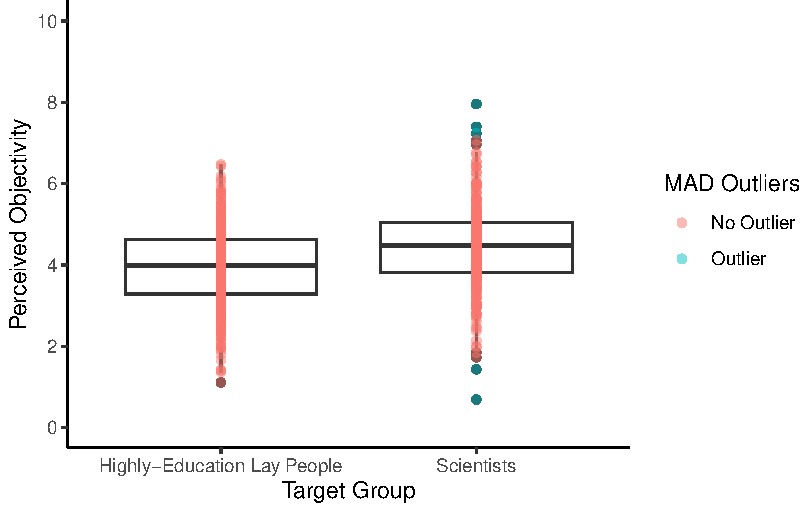
\includegraphics[width=1\textwidth,height=\textheight]{11-screening-data_files/figure-pdf/unnamed-chunk-23-1.pdf}
\end{center}

\textbf{Question 4}. If we fit a linear regression model, the effect of
group is

\begin{itemize}
\tightlist
\item
  \begin{enumerate}
  \def\labelenumi{(\Alph{enumi})}
  \tightlist
  \item
    statistically significant\\
  \end{enumerate}
\item
  \begin{enumerate}
  \def\labelenumi{(\Alph{enumi})}
  \setcounter{enumi}{1}
  \tightlist
  \item
    not statistically significant
  \end{enumerate}
\end{itemize}

and the

\begin{itemize}
\tightlist
\item
  \begin{enumerate}
  \def\labelenumi{(\Alph{enumi})}
  \tightlist
  \item
    highly-educated lay person\\
  \end{enumerate}
\item
  \begin{enumerate}
  \def\labelenumi{(\Alph{enumi})}
  \setcounter{enumi}{1}
  \tightlist
  \item
    scientist
  \end{enumerate}
\end{itemize}

scored higher on objectivity.

\begin{verbatim}

Call:
lm(formula = objectivity ~ group, data = df)

Residuals:
    Min      1Q  Median      3Q     Max 
-3.7514 -0.6257  0.0392  0.6479  3.5185 

Coefficients:
                Estimate Std. Error t value Pr(>|t|)    
(Intercept)      3.94113    0.05944  66.299  < 2e-16 ***
groupscientists  0.49932    0.08428   5.924 5.33e-09 ***
---
Signif. codes:  0 '***' 0.001 '**' 0.01 '*' 0.05 '.' 0.1 ' ' 1

Residual standard error: 1.024 on 589 degrees of freedom
  (9 observations deleted due to missingness)
Multiple R-squared:  0.05624,   Adjusted R-squared:  0.05464 
F-statistic:  35.1 on 1 and 589 DF,  p-value: 5.331e-09
\end{verbatim}

\textbf{Question 5}. If we check the modelling assumptions and focus on
normality and homoscedasticity, does it look like we meet the
assumptions for linear regression?

\begin{itemize}
\tightlist
\item
  \begin{enumerate}
  \def\labelenumi{(\Alph{enumi})}
  \tightlist
  \item
    Yes\\
  \end{enumerate}
\item
  \begin{enumerate}
  \def\labelenumi{(\Alph{enumi})}
  \setcounter{enumi}{1}
  \tightlist
  \item
    No
  \end{enumerate}
\end{itemize}

\begin{center}
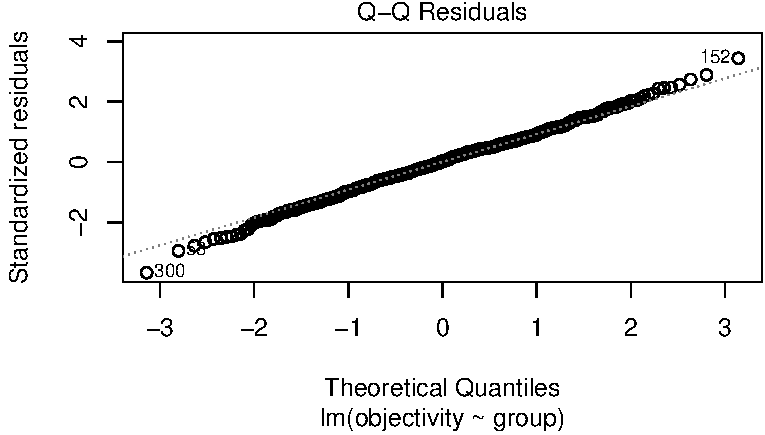
\includegraphics[width=1\textwidth,height=\textheight]{11-screening-data_files/figure-pdf/unnamed-chunk-25-1.pdf}
\end{center}

\begin{center}
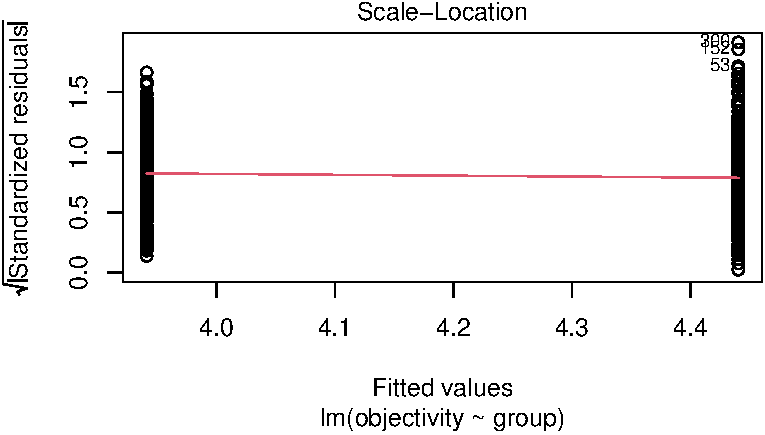
\includegraphics[width=1\textwidth,height=\textheight]{11-screening-data_files/figure-pdf/unnamed-chunk-25-2.pdf}
\end{center}

\begin{tcolorbox}[enhanced jigsaw, breakable, colframe=quarto-callout-caution-color-frame, arc=.35mm, opacitybacktitle=0.6, titlerule=0mm, colbacktitle=quarto-callout-caution-color!10!white, colback=white, toprule=.15mm, bottomtitle=1mm, toptitle=1mm, title=\textcolor{quarto-callout-caution-color}{\faFire}\hspace{0.5em}{Explain this answer}, bottomrule=.15mm, rightrule=.15mm, leftrule=.75mm, coltitle=black, left=2mm, opacityback=0]

For normality in the first plot, it does not look like there is a
significant deviation in expected values against observed values. We
have a few data points highlighted at the top and bottom of the points,
but there is not a consistent deviation to the pattern.

Likewise, for homoscedasticity in the second plot, the red line is
horizontal and there does not appear to be a noticeable difference in
the variance between each group.

\end{tcolorbox}

\textbf{Question 6}. If you were concerned about the presence of
potential outliers from question 3, are the regression results robust if
we remove those outliers?

\begin{itemize}
\tightlist
\item
  \begin{enumerate}
  \def\labelenumi{(\Alph{enumi})}
  \tightlist
  \item
    Yes\\
  \end{enumerate}
\item
  \begin{enumerate}
  \def\labelenumi{(\Alph{enumi})}
  \setcounter{enumi}{1}
  \tightlist
  \item
    No
  \end{enumerate}
\end{itemize}

\begin{verbatim}

Call:
lm(formula = objectivity ~ group, data = filter(df, obj_outlier == 
    "No Outlier"))

Residuals:
    Min      1Q  Median      3Q     Max 
-2.8339 -0.6167  0.0405  0.6370  2.6338 

Coefficients:
                Estimate Std. Error t value Pr(>|t|)    
(Intercept)      3.94113    0.05713  68.990  < 2e-16 ***
groupscientists  0.49062    0.08135   6.031 2.89e-09 ***
---
Signif. codes:  0 '***' 0.001 '**' 0.01 '*' 0.05 '.' 0.1 ' ' 1

Residual standard error: 0.9845 on 584 degrees of freedom
Multiple R-squared:  0.05864,   Adjusted R-squared:  0.05702 
F-statistic: 36.38 on 1 and 584 DF,  p-value: 2.887e-09
\end{verbatim}

\begin{tcolorbox}[enhanced jigsaw, breakable, colframe=quarto-callout-caution-color-frame, arc=.35mm, opacitybacktitle=0.6, titlerule=0mm, colbacktitle=quarto-callout-caution-color!10!white, colback=white, toprule=.15mm, bottomtitle=1mm, toptitle=1mm, title=\textcolor{quarto-callout-caution-color}{\faFire}\hspace{0.5em}{Explain this answer}, bottomrule=.15mm, rightrule=.15mm, leftrule=.75mm, coltitle=black, left=2mm, opacityback=0]

Yes, there is very little difference in the two results, so you would
confident the potential outliers are not driving the results. They are
both statistically significant and there is very little different in the
main effect size of interest, where the slope changes from 0.499 in
question 4 to 0.491 here.

\end{tcolorbox}

\section{Words from this Chapter}\label{words-from-this-chapter-10}

Below you will find a list of words that were used in this chapter that
might be new to you in case it helps to have somewhere to refer back to
what they mean. The links in this table take you to the entry for the
words in the \href{https://psyteachr.github.io/glossary/}{PsyTeachR
Glossary}. Note that the Glossary is written by numerous members of the
team and as such may use slightly different terminology from that shown
in the chapter.

\begin{longtable}[]{@{}
  >{\raggedright\arraybackslash}p{(\columnwidth - 2\tabcolsep) * \real{0.3264}}
  >{\raggedright\arraybackslash}p{(\columnwidth - 2\tabcolsep) * \real{0.6736}}@{}}
\toprule\noalign{}
\begin{minipage}[b]{\linewidth}\raggedright
term
\end{minipage} & \begin{minipage}[b]{\linewidth}\raggedright
definition
\end{minipage} \\
\midrule\noalign{}
\endhead
\bottomrule\noalign{}
\endlastfoot
\href{https://psyteachr.github.io/glossary/b\#binomial-distribution}{binomial-distribution}
& Instead of the parameters mean and standard deviation in a normal
distribution, you have \emph{N} trials with \emph{n} number of
successes. \\
\href{https://psyteachr.github.io/glossary/e\#error-outliers}{error-outliers}
& A mistake or impossible value in your data. \\
\href{https://psyteachr.github.io/glossary/i\#interesting-outliers}{interesting-outliers}
& Values in your data that looks extreme until you take another variable
or moderator into account. \\
\href{https://psyteachr.github.io/glossary/l\#logistic-regression}{logistic-regression}
& Modelling the log-odds of a dichotomous outcome as a linear
combination of one or more predictors. \\
\href{https://psyteachr.github.io/glossary/m\#missing-at-random}{missing-at-random}
& We can predict the missing value using other variables in the data. \\
\href{https://psyteachr.github.io/glossary/m\#missing-completely-at-random}{missing-completely-at-random}
& Whether the data are missing or not is completely unrelated to other
variables in the data. \\
\href{https://psyteachr.github.io/glossary/m\#missing-data}{missing-data}
& If a participant or observation contains no data for one or more
cells, they have missing data. \\
\href{https://psyteachr.github.io/glossary/m\#missing-not-at-random}{missing-not-at-random}
& Whether the data are missing or not is causally related to one or more
other variables in the data. \\
\href{https://psyteachr.github.io/glossary/r\#random-outliers}{random-outliers}
& Values in your data that are extreme compared to the majority of data
points. \\
\end{longtable}

\section{End of Chapter}\label{end-of-chapter-10}

That is the final chapter you will complete for the Research Methods 1
component of the course!

We hope you take a moment to think about everything you have achieved so
far. Think back to how you felt when you were completing Chapters 1 and
2 and learning what a function is. We must get through a huge amount of
content in a short space of time on the MSc conversion programmes, so we
hope you are all very proud in how far you have come. We cannot
guarantee everyone will come out of the course loving R and data skills,
but we hope you all recognise you \emph{can} do this.

The next few chapters you will cover in Research Methods 2, so make sure
you refresh your memory of the RM1 content prior to starting as the
topics build on what you already know around data skills and statistics.

\bookmarksetup{startatroot}

\chapter{One-way ANOVA}\label{one-way-anova}

This chapter marks the beginning of the content you cover in Research
Methods 2. You should be familiar with all the content from Research
Methods 1 we covered in Chapters 1 to 11, so please revisit previous
chapters if you need a refresher.

In the course materials, you have worked through manually calculating an
ANOVA to gain a conceptual understanding. However, when you run an
ANOVA, typically the computer does all of these calculations for you. In
this chapter, we will show you how to run a one-way ANOVA using the afex
package and post-hoc tests using the emmeans package.

\textbf{Chapter Intended Learning Outcomes (ILOs)}

By the end of this chapter, you will be able to:

\begin{itemize}
\item
  Apply and interpret a one-way ANOVA.
\item
  Break down the results of a one-way ANOVA using post-hocs tests and
  apply a correction for multiple comparisons.
\item
  Conduct a power analysis for a one-way ANOVA.
\end{itemize}

\section{Chapter preparation}\label{chapter-preparation-9}

\subsection{Introduction to the data
set}\label{introduction-to-the-data-set-7}

For this chapter, we are using open data from experiment 2 in James et
al. (2015). The abstract of their article is:

\begin{quote}
Memory of a traumatic event becomes consolidated within hours. Intrusive
memories can then flash back repeatedly into the mind's eye and cause
distress. We investigated whether reconsolidation - the process during
which memories become malleable when recalled - can be blocked using a
cognitive task and whether such an approach can reduce these unbidden
intrusions. We predicted that reconsolidation of a reactivated visual
memory of experimental trauma could be disrupted by engaging in a
visuospatial task that would compete for visual working memory
resources. We showed that intrusive memories were virtually abolished by
playing the computer game Tetris following a memory-reactivation task 24
hr after initial exposure to experimental trauma. Furthermore, both
memory reactivation and playing Tetris were required to reduce
subsequent intrusions (Experiment 2), consistent with
reconsolidation-update mechanisms. A simple, non-invasive cognitive-task
procedure administered after emotional memory has already consolidated
(i.e., \textgreater{} 24 hours after exposure to experimental trauma)
may prevent the recurrence of intrusive memories of those emotional
events.
\end{quote}

In summary, they were interested in whether you can reduce intrusive
memories associated with a traumatic event. Participants were randomly
allocated to one of four groups and watched a video designed to be
traumatic:

\begin{enumerate}
\def\labelenumi{\arabic{enumi}.}
\item
  Control
\item
  Reactivation + Tetris
\item
  Tetris
\item
  Reactivation
\end{enumerate}

They measured the number of intrusive memories prior to the start of the
study, then participants kept a diary to record intrusive memories about
the film in the 7 days after watching it. The authors were interested in
whether the combination of reactivation and playing Tetris would lead to
the largest reduction in intrusive memories. You will recreate their
analyses using a one-way ANOVA.

\subsection{Organising your files and project for the
chapter}\label{organising-your-files-and-project-for-the-chapter-9}

Before we can get started, you need to organise your files and project
for the chapter, so your working directory is in order.

\begin{enumerate}
\def\labelenumi{\arabic{enumi}.}
\item
  In your folder for research methods and the book
  \texttt{ResearchMethods1\_2/Quant\_Fundamentals}, create a new folder
  called \texttt{Chapter\_12\_ANOVA}. Within
  \texttt{Chapter\_12\_ANOVA}, create two new folders called
  \texttt{data} and \texttt{figures}.
\item
  Create an R Project for \texttt{Chapter\_12\_ANOVA} as an existing
  directory for your chapter folder. This should now be your working
  directory.
\item
  Create a new R Markdown document and give it a sensible title
  describing the chapter, such as \texttt{12\ ANOVA}. Delete everything
  below line 10 so you have a blank file to work with and save the file
  in your \texttt{Chapter\_12\_ANOVA} folder.
\item
  We are working with a new data set, so please save the following data
  file: \href{data/James_2015.csv}{James\_2015.csv}. Right click the
  link and select ``save link as'', or clicking the link will save the
  files to your Downloads. Make sure that you save the file as ``.csv''.
  Save or copy the file to your \texttt{data/} folder within
  \texttt{Chapter\_12\_ANOVA}.
\end{enumerate}

You are now ready to start working on the chapter!

\subsection{Activity 1 - Read and wrangle the
data}\label{activity-1---read-and-wrangle-the-data-4}

As the first activity, try and test yourself by completing the following
task list to practice your data wrangling skills. Create a final object
called \texttt{james\_data} to be consistent with the tasks below.

\begin{tcolorbox}[enhanced jigsaw, breakable, colframe=quarto-callout-tip-color-frame, arc=.35mm, opacitybacktitle=0.6, titlerule=0mm, colbacktitle=quarto-callout-tip-color!10!white, colback=white, toprule=.15mm, bottomtitle=1mm, toptitle=1mm, title=\textcolor{quarto-callout-tip-color}{\faLightbulb}\hspace{0.5em}{Try this}, bottomrule=.15mm, rightrule=.15mm, leftrule=.75mm, coltitle=black, left=2mm, opacityback=0]

To wrangle the data, complete the following tasks:

\begin{enumerate}
\def\labelenumi{\arabic{enumi}.}
\item
  Load the following packages (several of these are new, so revisit
  \hyperref[install-tidy]{Chapter 1} if you need a refresher of
  installing R packages, but remember not to install packages on the
  university computers / online server):

  \begin{itemize}
  \item
    pwr
  \item
    effectsize
  \item
    broom
  \item
    afex
  \item
    emmeans
  \item
    performance
  \item
    tidyverse
  \end{itemize}
\item
  Read the data file \texttt{data/James\_2015.csv} to the object name
  \texttt{james\_data}.
\item
  Create a new variable called \texttt{PID} that equals
  \texttt{row\_number()} to act as a participant ID which is currently
  missing from the data set.
\item
  Convert \texttt{Condition} to a factor.
\item
  Select and rename the following three variables as we do not need the
  others:

  \begin{itemize}
  \item
    \texttt{PID}
  \item
    \texttt{Condition}
  \item
    Rename
    \texttt{Days\_One\_to\_Seven\_Image\_Based\_Intrusions\_in\_Intrusion\_Diary}
    to \texttt{intrusions}.
  \end{itemize}
\end{enumerate}

\end{tcolorbox}

\begin{tcolorbox}[enhanced jigsaw, breakable, colframe=quarto-callout-caution-color-frame, arc=.35mm, opacitybacktitle=0.6, titlerule=0mm, colbacktitle=quarto-callout-caution-color!10!white, colback=white, toprule=.15mm, bottomtitle=1mm, toptitle=1mm, title=\textcolor{quarto-callout-caution-color}{\faFire}\hspace{0.5em}{Show me the solution}, bottomrule=.15mm, rightrule=.15mm, leftrule=.75mm, coltitle=black, left=2mm, opacityback=0]

You should have the following in a code chunk:

\begin{Shaded}
\begin{Highlighting}[]
\CommentTok{\# Load packages}
\FunctionTok{library}\NormalTok{(pwr)}
\FunctionTok{library}\NormalTok{(effectsize)}
\FunctionTok{library}\NormalTok{(broom)}
\FunctionTok{library}\NormalTok{(afex)}
\FunctionTok{library}\NormalTok{(emmeans)}
\FunctionTok{library}\NormalTok{(performance)}
\FunctionTok{library}\NormalTok{(tidyverse)}

\CommentTok{\# Read data and add new column}
\NormalTok{james\_data }\OtherTok{\textless{}{-}} \FunctionTok{read\_csv}\NormalTok{(}\StringTok{"data/James\_2015.csv"}\NormalTok{) }\SpecialCharTok{\%\textgreater{}\%}
  \FunctionTok{mutate}\NormalTok{(}\AttributeTok{PID =} \FunctionTok{row\_number}\NormalTok{(),}
         \AttributeTok{Condition =} \FunctionTok{as.factor}\NormalTok{(Condition)) }\SpecialCharTok{\%\textgreater{}\%} 
  \FunctionTok{select}\NormalTok{(PID, }
\NormalTok{         Condition, }
         \AttributeTok{intrusions =}\NormalTok{ Days\_One\_to\_Seven\_Image\_Based\_Intrusions\_in\_Intrusion\_Diary)}
\end{Highlighting}
\end{Shaded}

\end{tcolorbox}

\subsection{Activity 2 - Create summary statistics}\label{anova-a4}

Next, we want to calculate some descriptive statistics to see some
overall trends in the data. We are really interested in the scores from
each experimental group rather than overall.

\begin{tcolorbox}[enhanced jigsaw, breakable, colframe=quarto-callout-tip-color-frame, arc=.35mm, opacitybacktitle=0.6, titlerule=0mm, colbacktitle=quarto-callout-tip-color!10!white, colback=white, toprule=.15mm, bottomtitle=1mm, toptitle=1mm, title=\textcolor{quarto-callout-tip-color}{\faLightbulb}\hspace{0.5em}{Try this}, bottomrule=.15mm, rightrule=.15mm, leftrule=.75mm, coltitle=black, left=2mm, opacityback=0]

\begin{itemize}
\item
  Summarise the data to show the mean, standard deviation, and standard
  error for the number of intrusive memories (\texttt{intrusions})
  grouped by \texttt{Condition}.
\item
  Your table should have four columns, \texttt{Condition},
  \texttt{mean}, \texttt{sd}, and \texttt{se}.
\end{itemize}

Hint: You can calculate the standard error through: \texttt{sd/sqrt(n)}
or \texttt{sd/sqrt(length(some\_variable\_name)}.

\end{tcolorbox}

\begin{tcolorbox}[enhanced jigsaw, breakable, colframe=quarto-callout-caution-color-frame, arc=.35mm, opacitybacktitle=0.6, titlerule=0mm, colbacktitle=quarto-callout-caution-color!10!white, colback=white, toprule=.15mm, bottomtitle=1mm, toptitle=1mm, title=\textcolor{quarto-callout-caution-color}{\faFire}\hspace{0.5em}{Show me the solution}, bottomrule=.15mm, rightrule=.15mm, leftrule=.75mm, coltitle=black, left=2mm, opacityback=0]

You should have the following in a code chunk:

\begin{Shaded}
\begin{Highlighting}[]
\NormalTok{james\_data }\SpecialCharTok{\%\textgreater{}\%}
  \FunctionTok{group\_by}\NormalTok{(Condition) }\SpecialCharTok{\%\textgreater{}\%}
  \FunctionTok{summarise}\NormalTok{(}\AttributeTok{mean =} \FunctionTok{round}\NormalTok{(}\FunctionTok{mean}\NormalTok{(intrusions), }\DecValTok{2}\NormalTok{), }
            \AttributeTok{sd =} \FunctionTok{round}\NormalTok{(}\FunctionTok{sd}\NormalTok{(intrusions), }\DecValTok{2}\NormalTok{), }
            \AttributeTok{se =} \FunctionTok{round}\NormalTok{(sd}\SpecialCharTok{/}\FunctionTok{sqrt}\NormalTok{(}\FunctionTok{length}\NormalTok{(intrusions)), }\DecValTok{2}\NormalTok{))}
\end{Highlighting}
\end{Shaded}

\begin{verbatim}
# A tibble: 4 x 4
  Condition  mean    sd    se
  <fct>     <dbl> <dbl> <dbl>
1 1          5.11  4.23  1   
2 2          1.89  1.75  0.41
3 3          3.89  2.89  0.68
4 4          4.83  3.33  0.78
\end{verbatim}

\end{tcolorbox}

\subsection{Activity 3 - Visualisation}\label{anova-a5}

Now we can visualise the data. In the original paper they use a bar
plot, but let's use a better plot that gives us more information about
the data.

\begin{tcolorbox}[enhanced jigsaw, breakable, colframe=quarto-callout-tip-color-frame, arc=.35mm, opacitybacktitle=0.6, titlerule=0mm, colbacktitle=quarto-callout-tip-color!10!white, colback=white, toprule=.15mm, bottomtitle=1mm, toptitle=1mm, title=\textcolor{quarto-callout-tip-color}{\faLightbulb}\hspace{0.5em}{Try this}, bottomrule=.15mm, rightrule=.15mm, leftrule=.75mm, coltitle=black, left=2mm, opacityback=0]

\begin{itemize}
\item
  Create a violin-boxplot with the number of intrusive memories on the
  y-axis and condition on the x-axis (See Chapter 7 if you need a
  reminder).
\item
  Change the labels on the x-axis to something more informative for the
  condition names.
\end{itemize}

Your plot should look like this:

\begin{center}
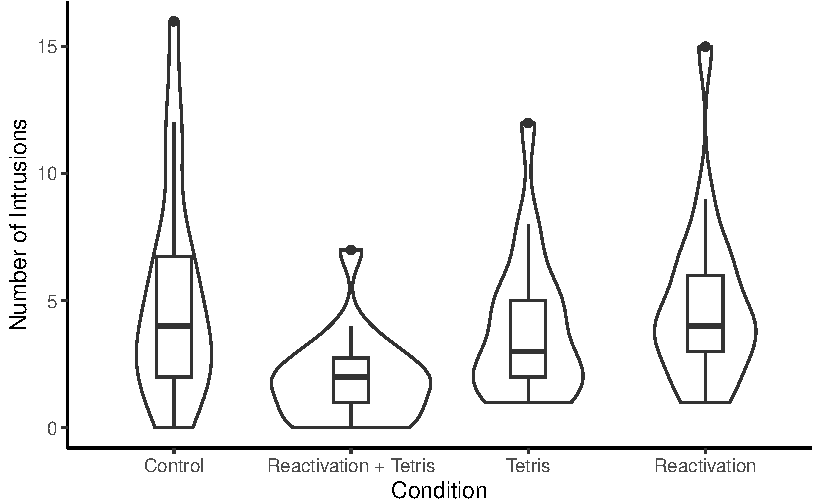
\includegraphics[width=1\textwidth,height=\textheight]{12-anova_files/figure-pdf/unnamed-chunk-3-1.pdf}
\end{center}

\end{tcolorbox}

\begin{tcolorbox}[enhanced jigsaw, breakable, colframe=quarto-callout-caution-color-frame, arc=.35mm, opacitybacktitle=0.6, titlerule=0mm, colbacktitle=quarto-callout-caution-color!10!white, colback=white, toprule=.15mm, bottomtitle=1mm, toptitle=1mm, title=\textcolor{quarto-callout-caution-color}{\faFire}\hspace{0.5em}{Show me the solution}, bottomrule=.15mm, rightrule=.15mm, leftrule=.75mm, coltitle=black, left=2mm, opacityback=0]

You should have the following in a code chunk:

\begin{Shaded}
\begin{Highlighting}[]
\NormalTok{james\_data }\SpecialCharTok{\%\textgreater{}\%} 
  \FunctionTok{ggplot}\NormalTok{(}\FunctionTok{aes}\NormalTok{(}\AttributeTok{x =}\NormalTok{ Condition, }\AttributeTok{y =}\NormalTok{ intrusions))}\SpecialCharTok{+}
  \FunctionTok{geom\_violin}\NormalTok{()}\SpecialCharTok{+}
  \FunctionTok{geom\_boxplot}\NormalTok{(}\AttributeTok{width =}\NormalTok{ .}\DecValTok{2}\NormalTok{) }\SpecialCharTok{+} 
  \FunctionTok{scale\_y\_continuous}\NormalTok{(}\AttributeTok{name =} \StringTok{"Number of Intrusions"}\NormalTok{) }\SpecialCharTok{+} 
  \FunctionTok{scale\_x\_discrete}\NormalTok{(}\AttributeTok{labels =} \FunctionTok{c}\NormalTok{(}\StringTok{"Control"}\NormalTok{, }\StringTok{"Reactivation + Tetris"}\NormalTok{, }\StringTok{"Tetris"}\NormalTok{, }\StringTok{"Reactivation"}\NormalTok{)) }\SpecialCharTok{+} 
  \FunctionTok{theme\_classic}\NormalTok{()}
\end{Highlighting}
\end{Shaded}

We can see from this plot that there are a few potential outliers in
each of the groups. This information is not present in the bar plot,
which is why it's not a good idea to use them for this kind of data.

\end{tcolorbox}

\section{One-way ANOVA}\label{anova-a6}

Now we can run the one-way ANOVA using \texttt{aov\_ez()} from the afex
package and save it to the object \texttt{mod}. As well as running the
ANOVA, the \texttt{aov\_ez()} function also conducts a Levene's test for
homogeneity of variance so that we can test our final assumption.

\subsection{Activity 4 - Running a one-way ANOVA using
afex}\label{activity-4---running-a-one-way-anova-using-afex}

\texttt{aov\_ez()} will likely produce some messages that look like
errors, do not worry about these, they are just letting you know what
it's done. Run the code below to view the results of the ANOVA.

\begin{Shaded}
\begin{Highlighting}[]
\NormalTok{mod }\OtherTok{\textless{}{-}} \FunctionTok{aov\_ez}\NormalTok{(}\AttributeTok{id =} \StringTok{"PID"}\NormalTok{, }\CommentTok{\# the column containing the participant IDs}
              \AttributeTok{dv =} \StringTok{"intrusions"}\NormalTok{, }\CommentTok{\# the DV }
              \AttributeTok{between =} \StringTok{"Condition"}\NormalTok{, }\CommentTok{\# the between{-}subject variable}
              \AttributeTok{es =} \StringTok{"pes"}\NormalTok{, }\CommentTok{\# sets effect size to partial eta{-}squared}
              \AttributeTok{type =} \DecValTok{3}\NormalTok{, }\CommentTok{\# this affects how the sum of squares is calculated, set this to 3}
              \AttributeTok{include\_aov =} \ConstantTok{TRUE}\NormalTok{,}
              \AttributeTok{data =}\NormalTok{ james\_data)}

\NormalTok{mod}
\end{Highlighting}
\end{Shaded}

\begin{verbatim}
Anova Table (Type 3 tests)

Response: intrusions
     Effect    df   MSE      F  ges p.value
1 Condition 3, 68 10.09 3.79 * .143    .014
---
Signif. codes:  0 '***' 0.001 '**' 0.01 '*' 0.05 '+' 0.1 ' ' 1
\end{verbatim}

Just like with the t-tests and correlations, we can use \texttt{tidy()}
to make the output easier to work with. Run the below code to transform
the output. Do not worry about the warning message, it is just telling
you it does not know how to automatically rename the columns so it will
keep the original names.

\begin{Shaded}
\begin{Highlighting}[]
\NormalTok{mod\_output }\OtherTok{\textless{}{-}}\NormalTok{ mod}\SpecialCharTok{$}\NormalTok{anova\_table }\SpecialCharTok{\%\textgreater{}\%} 
  \FunctionTok{tidy}\NormalTok{()}
\end{Highlighting}
\end{Shaded}

\begin{verbatim}
Warning in tidy.anova(.): The following column names in ANOVA output were not
recognized or transformed: num.Df, den.Df, MSE, ges
\end{verbatim}

\begin{Shaded}
\begin{Highlighting}[]
\NormalTok{mod\_output}
\end{Highlighting}
\end{Shaded}

\begin{verbatim}
# A tibble: 1 x 7
  term      num.Df den.Df   MSE statistic   ges p.value
  <chr>      <dbl>  <dbl> <dbl>     <dbl> <dbl>   <dbl>
1 Condition      3     68  10.1      3.79 0.143  0.0141
\end{verbatim}

\begin{itemize}
\tightlist
\item
  \texttt{term} = the IV\\
\item
  \texttt{num.Df} = degrees of freedom effect
\item
  \texttt{den.Df} = degrees of freedom residuals
\item
  \texttt{MSE} = Mean-squared errors
\item
  \texttt{statistic} = F-statistic
\item
  \texttt{ges} = effect size\\
\item
  \texttt{p.value} = p.value
\end{itemize}

You should refer to the lecture for more information on what each
variable means and how it is calculated.

\begin{itemize}
\item
  Is the overall effect of Condition significant?
\item
  \begin{enumerate}
  \def\labelenumi{(\Alph{enumi})}
  \tightlist
  \item
    Yes\\
  \end{enumerate}
\item
  \begin{enumerate}
  \def\labelenumi{(\Alph{enumi})}
  \setcounter{enumi}{1}
  \tightlist
  \item
    No
  \end{enumerate}
\item
  What is the F-statistics to 2 decimal places? \_\_\_\_
\item
  According to the rules of thumb, the effect size is
\item
  \begin{enumerate}
  \def\labelenumi{(\Alph{enumi})}
  \tightlist
  \item
    Small\\
  \end{enumerate}
\item
  \begin{enumerate}
  \def\labelenumi{(\Alph{enumi})}
  \setcounter{enumi}{1}
  \tightlist
  \item
    Medium\\
  \end{enumerate}
\item
  \begin{enumerate}
  \def\labelenumi{(\Alph{enumi})}
  \setcounter{enumi}{2}
  \tightlist
  \item
    Large
  \end{enumerate}
\end{itemize}

\subsection{Activity 5 - Checking assumptions for ANOVA}\label{anova-a7}

To test the assumptions, we must use the model we created with
\texttt{aov\_ez()}. For a one-way independent ANOVA, the assumptions are
the same as for a Student t-test / regression model with a categorical
predictor:

\begin{enumerate}
\def\labelenumi{\arabic{enumi}.}
\item
  The DV is interval or ratio data.
\item
  The observations should be independent.
\item
  The residuals should be normally distributed.
\item
  There should be homogeneity of variance between the groups.
\end{enumerate}

We know that 1 and 2 are met because of the design of our study. To test
3, we can look at the qq-plot of the residuals. Instead of saving just
the model object, we must specifically select the \texttt{aov} component
and run our diagnostic plots.

\begin{Shaded}
\begin{Highlighting}[]
\FunctionTok{plot}\NormalTok{(mod}\SpecialCharTok{$}\NormalTok{aov, }
     \AttributeTok{which =} \DecValTok{2}\NormalTok{)}
\end{Highlighting}
\end{Shaded}

\begin{figure}[H]

\centering{

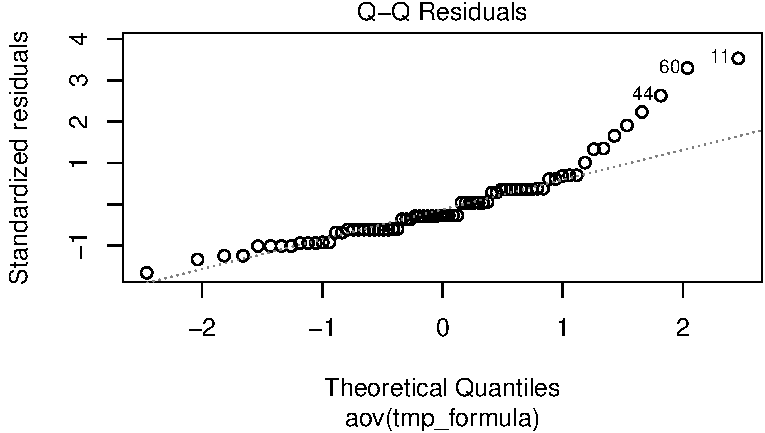
\includegraphics[width=1\textwidth,height=\textheight]{12-anova_files/figure-pdf/fig-qq-1.pdf}

}

\caption{\label{fig-qq}qq-plot for model residuals.}

\end{figure}%

The qq-plot shows the assumption of normality might not be ideal. Is
this a problem? If the sample sizes for each group are equal, then ANOVA
is robust to violations of both normality and of homogeneity of
variance. If you are interested, there is a good discussion of these
issues in Blanca et al. (2018) and Knief \& Forstmeier (2021). We can
check how many participants are in each condition using
\texttt{count()}:

\begin{Shaded}
\begin{Highlighting}[]
\NormalTok{james\_data }\SpecialCharTok{\%\textgreater{}\%} 
  \FunctionTok{count}\NormalTok{(Condition)}
\end{Highlighting}
\end{Shaded}

\begin{verbatim}
# A tibble: 4 x 2
  Condition     n
  <fct>     <int>
1 1            18
2 2            18
3 3            18
4 4            18
\end{verbatim}

Thankfully, the sample sizes are equal, so we should be OK to proceed
with the ANOVA. It is not clear whether normality was checked in the
original paper.

For the last assumption, we can test homogeneity of variance by checking
the third diagnostic plot for the scale against location.

\begin{Shaded}
\begin{Highlighting}[]
\FunctionTok{plot}\NormalTok{(mod}\SpecialCharTok{$}\NormalTok{aov, }
     \AttributeTok{which =} \DecValTok{3}\NormalTok{)}
\end{Highlighting}
\end{Shaded}

\begin{figure}[H]

\centering{

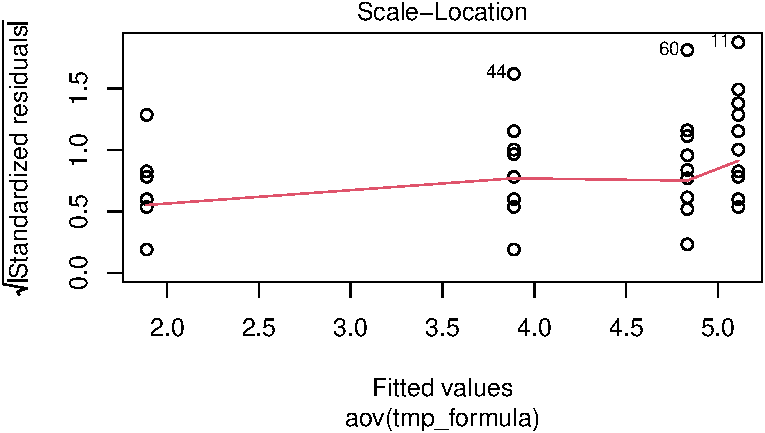
\includegraphics[width=1\textwidth,height=\textheight]{12-anova_files/figure-pdf/fig-homogeneity-1.pdf}

}

\caption{\label{fig-homogeneity}Diagnostic plot for homogeneity of
variance.}

\end{figure}%

Compared to normality, this assumption looks closer to being supported
as the variance of each group is approximately equal. James et al.
(2015) suspect there might be issues with this assumption as they
mention that the ANOVAs do not assume equal variance, however, the
results of the ANOVA that are reported are identical to our results
above where no correction has been made although the post-hoc tests are
Welch t-tests (you can tell this because the degrees of freedom have
been adjusted and are not whole numbers).

While all of this might seem very confusing - we imagine you might be
wondering what the point of assumption testing is given that it seems to
be ignored - we are showing you this for three reasons:

\begin{enumerate}
\def\labelenumi{\arabic{enumi}.}
\item
  To reassure you that sometimes the data can fail to meet the
  assumptions and it is still ok to use the test. To put this in
  statistical terms, many tests are \textbf{robust} to mild deviations
  of normality and unequal variance, particularly with equal sample
  sizes.
\item
  As a critical thinking point, to remind you that just because a piece
  of research has been published does not mean it is perfect and you
  should always evaluate whether the methods used are appropriate.
\item
  To reinforce the importance of pre-registration where these decisions
  could be made in advance, and/or open data and code so that analyses
  can be reproduced exactly to avoid any ambiguity about exactly what
  was done. In this example, given the equal sample sizes and the
  difference in variance between the groups isn't too extreme, it looks
  like it is still appropriate to use an ANOVA but the decisions and
  justification for those decisions could have been more transparent.
\end{enumerate}

\begin{tcolorbox}[enhanced jigsaw, breakable, colframe=quarto-callout-note-color-frame, arc=.35mm, opacitybacktitle=0.6, titlerule=0mm, colbacktitle=quarto-callout-note-color!10!white, colback=white, toprule=.15mm, bottomtitle=1mm, toptitle=1mm, title=\textcolor{quarto-callout-note-color}{\faInfo}\hspace{0.5em}{Note}, bottomrule=.15mm, rightrule=.15mm, leftrule=.75mm, coltitle=black, left=2mm, opacityback=0]

The \texttt{check\_model()} function from performance also works here,
so you can see what it looks like if you run:

\begin{Shaded}
\begin{Highlighting}[]
\FunctionTok{check\_model}\NormalTok{(mod}\SpecialCharTok{$}\NormalTok{aov)}
\end{Highlighting}
\end{Shaded}

\end{tcolorbox}

\subsection{Activity 6 - Post-hoc tests}\label{anova-a8}

For post-hoc comparisons, the paper appears to have computed Welch
t-tests but there is no mention of any multiple comparison correction.
We could reproduce these results by using \texttt{t.test()} for each of
the contrasts.

For example, to compare condition 1 (the control group) with condition 2
(the reactivation plus tetris group) we could run:

\begin{Shaded}
\begin{Highlighting}[]
\NormalTok{james\_data }\SpecialCharTok{\%\textgreater{}\%}
  \FunctionTok{filter}\NormalTok{(Condition }\SpecialCharTok{\%in\%} \FunctionTok{c}\NormalTok{(}\StringTok{"1"}\NormalTok{, }\StringTok{"2"}\NormalTok{)) }\SpecialCharTok{\%\textgreater{}\%}
  \FunctionTok{droplevels}\NormalTok{() }\SpecialCharTok{\%\textgreater{}\%} \CommentTok{\# ignore unused factor levels}
  \FunctionTok{t.test}\NormalTok{(intrusions }\SpecialCharTok{\textasciitilde{}}\NormalTok{ Condition, }
         \AttributeTok{data =}\NormalTok{ .)}
\end{Highlighting}
\end{Shaded}

\begin{verbatim}

    Welch Two Sample t-test

data:  intrusions by Condition
t = 2.9893, df = 22.632, p-value = 0.006627
alternative hypothesis: true difference in means between group 1 and group 2 is not equal to 0
95 percent confidence interval:
 0.990331 5.454113
sample estimates:
mean in group 1 mean in group 2 
       5.111111        1.888889 
\end{verbatim}

\begin{tcolorbox}[enhanced jigsaw, breakable, colframe=quarto-callout-important-color-frame, arc=.35mm, opacitybacktitle=0.6, titlerule=0mm, colbacktitle=quarto-callout-important-color!10!white, colback=white, toprule=.15mm, bottomtitle=1mm, toptitle=1mm, title=\textcolor{quarto-callout-important-color}{\faExclamation}\hspace{0.5em}{Important}, bottomrule=.15mm, rightrule=.15mm, leftrule=.75mm, coltitle=black, left=2mm, opacityback=0]

Because \texttt{Condition} has four levels, we cannot just specify
\texttt{intrustion\ \textasciitilde{}\ Condition} because a t-test
compares two groups and it would not know which of the four to compare
so first we have to filter the data and use a new function
\texttt{droplevels()}. It's important to remember that when it comes to
R there are two things to consider, the data you can see and the
underlying structure of that data. In the above code we use
\texttt{filter()} to select only conditions 1 and 2 so that we can
compare them. However, that does not change the fact that R ``knows''
that \texttt{Condition} has four levels - it does not matter if two of
those levels do not have any observations any more, the underlying
structure still says there are four groups. \texttt{droplevels()} tells
R to remove any unused levels from a factor. Try running the above code
but without \texttt{droplevels()} and see what happens.

\end{tcolorbox}

However, a quicker and better way of doing this that allows you apply a
correction for multiple comparisons easily is to use \texttt{emmeans()}
which computes all possible pairwise comparison t-tests and applies a
correction to the p-value.

First, we use \texttt{emmeans()} to run the comparisons and then we can
pull out the contrasts and use \texttt{tidy()} to make it easier to work
with.

Run the code below. Which conditions are significantly different from
each other? Are any of the comparisons different from the ones reported
in the paper now that a correction for multiple comparisons has been
applied?

\begin{Shaded}
\begin{Highlighting}[]
\NormalTok{mod\_pairwise }\OtherTok{\textless{}{-}}\FunctionTok{emmeans}\NormalTok{(mod, }
\NormalTok{                       pairwise }\SpecialCharTok{\textasciitilde{}}\NormalTok{ Condition, }
                       \AttributeTok{adjust =} \StringTok{"bonferroni"}\NormalTok{)}

\NormalTok{mod\_contrasts }\OtherTok{\textless{}{-}}\NormalTok{ mod\_pairwise}\SpecialCharTok{$}\NormalTok{contrasts }\SpecialCharTok{\%\textgreater{}\%} 
  \FunctionTok{tidy}\NormalTok{()}

\NormalTok{mod\_contrasts}
\end{Highlighting}
\end{Shaded}

\begin{verbatim}
# A tibble: 6 x 8
  term      contrast   null.value estimate std.error    df statistic adj.p.value
  <chr>     <chr>           <dbl>    <dbl>     <dbl> <dbl>     <dbl>       <dbl>
1 Condition Condition~          0    3.22       1.06    68     3.04       0.0199
2 Condition Condition~          0    1.22       1.06    68     1.15       1     
3 Condition Condition~          0    0.278      1.06    68     0.262      1     
4 Condition Condition~          0   -2.00       1.06    68    -1.89       0.379 
5 Condition Condition~          0   -2.94       1.06    68    -2.78       0.0420
6 Condition Condition~          0   -0.944      1.06    68    -0.892      1     
\end{verbatim}

\begin{tcolorbox}[enhanced jigsaw, breakable, colframe=quarto-callout-warning-color-frame, arc=.35mm, opacitybacktitle=0.6, titlerule=0mm, colbacktitle=quarto-callout-warning-color!10!white, colback=white, toprule=.15mm, bottomtitle=1mm, toptitle=1mm, title=\textcolor{quarto-callout-warning-color}{\faExclamationTriangle}\hspace{0.5em}{Warning}, bottomrule=.15mm, rightrule=.15mm, leftrule=.75mm, coltitle=black, left=2mm, opacityback=0]

The inquisitive among you may have noticed that \texttt{mod} is a list
of 5 and seemingly contains the same thing three times:
\texttt{anova\_table}, \texttt{aov} and \texttt{Anova}. The reasons
behind the differences are too complex to go into detail on this course
(see The R Companion
\href{https://rcompanion.org/rcompanion/d_04.html}{website here} for
more information) but the simple version is that \texttt{anova\_table}
and \texttt{Anova} use one method of calculating the results (type 3 sum
of squares) and \texttt{aov} uses a different method (type 1 sum of
squares). What's important for your purposes is that you need to use
\texttt{anova\_table} to view the overall results (and replicate the
results from papers) and \texttt{aov}to run the follow-up tests and to
get access to the residuals (or \texttt{lm()} for factorial ANOVA). As
always, precision and attention to detail is key.

\end{tcolorbox}

\subsection{Activity 7 - Power and effect sizes}\label{anova-a9}

Finally, we can replicate their power analysis using
\texttt{pwr.anova.test}from the pwr package.

\begin{quote}
On the basis of the effect size of d = 1.14 from Experiment 1, we
assumed a large effect size of f = 0.4. A sample size of 18 per
condition was required in order to ensure an 80\% power to detect this
difference at the 5\% significance level.
\end{quote}

\begin{Shaded}
\begin{Highlighting}[]
\FunctionTok{pwr.anova.test}\NormalTok{(}\AttributeTok{k =} \DecValTok{4}\NormalTok{, }
               \AttributeTok{f =}\NormalTok{ .}\DecValTok{4}\NormalTok{, }
               \AttributeTok{sig.level =}\NormalTok{ .}\DecValTok{05}\NormalTok{, }
               \AttributeTok{power =}\NormalTok{ .}\DecValTok{8}\NormalTok{)}
\end{Highlighting}
\end{Shaded}

\begin{verbatim}

     Balanced one-way analysis of variance power calculation 

              k = 4
              n = 18.04262
              f = 0.4
      sig.level = 0.05
          power = 0.8

NOTE: n is number in each group
\end{verbatim}

We have already got the effect size for the overall ANOVA, however, we
should also really calculate Cohen's d using \texttt{cohens\_d()} from
effectsize for each of the pairwise comparisons. This code is a little
long because you need to do it separately for each comparison, bind them
all together and then add them to \texttt{mod\_contrasts} - just make
sure your understand which bits of the code you would need to change to
run this on different data. As we are binding rows and columns rather
than joining, it is critical the comparisons are already in the correct
order.

\begin{Shaded}
\begin{Highlighting}[]
\CommentTok{\# Calculate Cohen\textquotesingle{}s d for all comparisons}
\NormalTok{d\_1\_2 }\OtherTok{\textless{}{-}} \FunctionTok{cohens\_d}\NormalTok{(intrusions }\SpecialCharTok{\textasciitilde{}}\NormalTok{ Condition, }
                 \AttributeTok{data =} \FunctionTok{filter}\NormalTok{(james\_data, }
\NormalTok{                               Condition }\SpecialCharTok{\%in\%} \FunctionTok{c}\NormalTok{(}\DecValTok{1}\NormalTok{, }\DecValTok{2}\NormalTok{)) }\SpecialCharTok{\%\textgreater{}\%} 
                   \FunctionTok{droplevels}\NormalTok{())}

\NormalTok{d\_1\_3 }\OtherTok{\textless{}{-}} \FunctionTok{cohens\_d}\NormalTok{(intrusions }\SpecialCharTok{\textasciitilde{}}\NormalTok{ Condition, }
                 \AttributeTok{data =} \FunctionTok{filter}\NormalTok{(james\_data, }
\NormalTok{                               Condition }\SpecialCharTok{\%in\%} \FunctionTok{c}\NormalTok{(}\DecValTok{1}\NormalTok{, }\DecValTok{3}\NormalTok{)) }\SpecialCharTok{\%\textgreater{}\%} 
                   \FunctionTok{droplevels}\NormalTok{()) }

\NormalTok{d\_1\_4 }\OtherTok{\textless{}{-}} \FunctionTok{cohens\_d}\NormalTok{(intrusions }\SpecialCharTok{\textasciitilde{}}\NormalTok{ Condition, }
                 \AttributeTok{data =} \FunctionTok{filter}\NormalTok{(james\_data, }
\NormalTok{                               Condition }\SpecialCharTok{\%in\%} \FunctionTok{c}\NormalTok{(}\DecValTok{1}\NormalTok{, }\DecValTok{4}\NormalTok{)) }\SpecialCharTok{\%\textgreater{}\%} 
                   \FunctionTok{droplevels}\NormalTok{())}

\NormalTok{d\_2\_3 }\OtherTok{\textless{}{-}} \FunctionTok{cohens\_d}\NormalTok{(intrusions }\SpecialCharTok{\textasciitilde{}}\NormalTok{ Condition, }
                 \AttributeTok{data =} \FunctionTok{filter}\NormalTok{(james\_data, }
\NormalTok{                               Condition }\SpecialCharTok{\%in\%} \FunctionTok{c}\NormalTok{(}\DecValTok{2}\NormalTok{, }\DecValTok{3}\NormalTok{)) }\SpecialCharTok{\%\textgreater{}\%} 
                   \FunctionTok{droplevels}\NormalTok{())}

\NormalTok{d\_2\_4 }\OtherTok{\textless{}{-}} \FunctionTok{cohens\_d}\NormalTok{(intrusions }\SpecialCharTok{\textasciitilde{}}\NormalTok{ Condition, }
                 \AttributeTok{data =} \FunctionTok{filter}\NormalTok{(james\_data, }
\NormalTok{                               Condition }\SpecialCharTok{\%in\%} \FunctionTok{c}\NormalTok{(}\DecValTok{2}\NormalTok{, }\DecValTok{4}\NormalTok{)) }\SpecialCharTok{\%\textgreater{}\%} 
                   \FunctionTok{droplevels}\NormalTok{())}

\NormalTok{d\_3\_4 }\OtherTok{\textless{}{-}} \FunctionTok{cohens\_d}\NormalTok{(intrusions }\SpecialCharTok{\textasciitilde{}}\NormalTok{ Condition, }
                 \AttributeTok{data =} \FunctionTok{filter}\NormalTok{(james\_data, }
\NormalTok{                               Condition }\SpecialCharTok{\%in\%} \FunctionTok{c}\NormalTok{(}\DecValTok{3}\NormalTok{, }\DecValTok{4}\NormalTok{)) }\SpecialCharTok{\%\textgreater{}\%} 
                   \FunctionTok{droplevels}\NormalTok{())}

\CommentTok{\# Bind all the comparisons in the order of mod\_contrasts}
\NormalTok{pairwise\_ds }\OtherTok{\textless{}{-}} \FunctionTok{bind\_rows}\NormalTok{(d\_1\_2, }
\NormalTok{                         d\_1\_3, }
\NormalTok{                         d\_1\_4,}
\NormalTok{                         d\_2\_3, }
\NormalTok{                         d\_2\_4, }
\NormalTok{                         d\_3\_4)}

\CommentTok{\# Bind this object to the mod\_contrasts object}
\NormalTok{mod\_contrasts }\OtherTok{\textless{}{-}}\NormalTok{ mod\_contrasts }\SpecialCharTok{\%\textgreater{}\%}
  \FunctionTok{bind\_cols}\NormalTok{(pairwise\_ds)}
\end{Highlighting}
\end{Shaded}

\begin{tcolorbox}[enhanced jigsaw, breakable, colframe=quarto-callout-warning-color-frame, arc=.35mm, opacitybacktitle=0.6, titlerule=0mm, colbacktitle=quarto-callout-warning-color!10!white, colback=white, toprule=.15mm, bottomtitle=1mm, toptitle=1mm, title=\textcolor{quarto-callout-warning-color}{\faExclamationTriangle}\hspace{0.5em}{Warning}, bottomrule=.15mm, rightrule=.15mm, leftrule=.75mm, coltitle=black, left=2mm, opacityback=0]

What are your options if the data do not meet the assumptions and it's
really not appropriate to continue with a regular one-way ANOVA? As
always, there are multiple options and it is a judgement call.

\begin{enumerate}
\def\labelenumi{\arabic{enumi}.}
\item
  You could run a non-parametric test, the Kruskal-Wallis for
  between-subject designs and the Friedman test for within-subject
  designs.
\item
  If normality is the problem, you could try transforming the data.
\item
  You could use bootstrapping, which is not something we will cover in
  this course at all.
\end{enumerate}

\end{tcolorbox}

\section{Reporting the results of your ANOVA}\label{anova-a10}

The below code replicates the write-up in the paper, although has
changed the Welch t-test to the pairwise comparisons from
\texttt{emmeans()}.

\begin{Shaded}
\begin{Highlighting}[]
\NormalTok{Second, and critically, }\ControlFlowTok{for}\NormalTok{ the }\DecValTok{7}\SpecialCharTok{{-}}\NormalTok{day diary postintervention, there was a significant difference between groups }\ControlFlowTok{in}\NormalTok{ overall intrusion frequency }\ControlFlowTok{in}\NormalTok{ daily life, }\FunctionTok{F}\NormalTok{(}\StringTok{\textasciigrave{}}\AttributeTok{r mod\_output$num.Df}\StringTok{\textasciigrave{}}\NormalTok{, }\StringTok{\textasciigrave{}}\AttributeTok{r mod\_output$den.Df}\StringTok{\textasciigrave{}}\NormalTok{) }\OtherTok{=} \StringTok{\textasciigrave{}}\AttributeTok{r mod\_output$statistic \%\textgreater{}\% round(2)}\StringTok{\textasciigrave{}}\NormalTok{, p }\OtherTok{=} \StringTok{\textasciigrave{}}\AttributeTok{r mod\_output$p.value \%\textgreater{}\% round(3)}\StringTok{\textasciigrave{}}\NormalTok{, ηp2 }\OtherTok{=}\NormalTok{ .}\StringTok{\textasciigrave{}}\AttributeTok{r mod\_output$ges \%\textgreater{}\% round(2)}\StringTok{\textasciigrave{}}\NormalTok{. Planned comparisons demonstrated that relative to the no}\SpecialCharTok{{-}}\NormalTok{task control group, only those }\ControlFlowTok{in}\NormalTok{ the reactivation}\SpecialCharTok{{-}}\NormalTok{plus}\SpecialCharTok{{-}}\NormalTok{Tetris group, }\FunctionTok{t}\NormalTok{(}\StringTok{\textasciigrave{}}\AttributeTok{r mod\_contrasts$df[1]}\StringTok{\textasciigrave{}}\NormalTok{) }\OtherTok{=} \StringTok{\textasciigrave{}}\AttributeTok{r mod\_contrasts$statistic[1] \%\textgreater{}\% round(2)}\StringTok{\textasciigrave{}}\NormalTok{, p }\OtherTok{=} \StringTok{\textasciigrave{}}\AttributeTok{r mod\_contrasts$adj.p.value[1] \%\textgreater{}\% round(2)}\StringTok{\textasciigrave{}}\NormalTok{, d }\OtherTok{=} \StringTok{\textasciigrave{}}\AttributeTok{r mod\_contrasts$Cohens\_d[1] \%\textgreater{}\% round(2)}\StringTok{\textasciigrave{}}\NormalTok{, experienced significantly fewer intrusive memories; this finding replicated Experiment }\FloatTok{1.}\NormalTok{ The reactivation}\SpecialCharTok{{-}}\NormalTok{plus}\SpecialCharTok{{-}}\NormalTok{Tetris group had significantly fewer intrusive thoughts than the reactivation}\SpecialCharTok{{-}}\NormalTok{only group, }\FunctionTok{t}\NormalTok{(}\StringTok{\textasciigrave{}}\AttributeTok{r mod\_contrasts$df[5]}\StringTok{\textasciigrave{}}\NormalTok{) }\OtherTok{=} \StringTok{\textasciigrave{}}\AttributeTok{r mod\_contrasts$statistic[5] \%\textgreater{}\% round(2)}\StringTok{\textasciigrave{}}\NormalTok{, p }\OtherTok{=} \StringTok{\textasciigrave{}}\AttributeTok{r mod\_contrasts$adj.p.value[5] \%\textgreater{}\% round(2)}\StringTok{\textasciigrave{}}\NormalTok{, d }\OtherTok{=} \StringTok{\textasciigrave{}}\AttributeTok{r mod\_contrasts$Cohens\_d[5] \%\textgreater{}\% round(2)}\StringTok{\textasciigrave{}}\NormalTok{. Further, there were no significant differences between the reactivation}\SpecialCharTok{{-}}\NormalTok{plus}\SpecialCharTok{{-}}\NormalTok{Tetris group and the Tetris}\SpecialCharTok{{-}}\NormalTok{only group, }\FunctionTok{t}\NormalTok{(}\StringTok{\textasciigrave{}}\AttributeTok{r mod\_contrasts$df[4]}\StringTok{\textasciigrave{}}\NormalTok{) }\OtherTok{=} \StringTok{\textasciigrave{}}\AttributeTok{r mod\_contrasts$statistic[4] \%\textgreater{}\% round(2)}\StringTok{\textasciigrave{}}\NormalTok{, p }\OtherTok{=} \StringTok{\textasciigrave{}}\AttributeTok{r mod\_contrasts$adj.p.value[4] \%\textgreater{}\% round(2)}\StringTok{\textasciigrave{}}\NormalTok{, d }\OtherTok{=} \StringTok{\textasciigrave{}}\AttributeTok{r mod\_contrasts$Cohens\_d[4] \%\textgreater{}\% round(2)}\StringTok{\textasciigrave{}}\NormalTok{, the no}\SpecialCharTok{{-}}\NormalTok{task control group and the reactivation}\SpecialCharTok{{-}}\NormalTok{only group, }\FunctionTok{t}\NormalTok{(}\StringTok{\textasciigrave{}}\AttributeTok{r mod\_contrasts$df[3]}\StringTok{\textasciigrave{}}\NormalTok{) }\OtherTok{=} \StringTok{\textasciigrave{}}\AttributeTok{r mod\_contrasts$statistic[3] \%\textgreater{}\% round(2)}\StringTok{\textasciigrave{}}\NormalTok{, p }\OtherTok{=} \StringTok{\textasciigrave{}}\AttributeTok{r mod\_contrasts$adj.p.value[3] \%\textgreater{}\% round(2)}\StringTok{\textasciigrave{}}\NormalTok{, or between the no}\SpecialCharTok{{-}}\NormalTok{task control group and the Tetris}\SpecialCharTok{{-}}\NormalTok{only group, }\FunctionTok{t}\NormalTok{(}\StringTok{\textasciigrave{}}\AttributeTok{r mod\_contrasts$df[2]}\StringTok{\textasciigrave{}}\NormalTok{) }\OtherTok{=} \StringTok{\textasciigrave{}}\AttributeTok{r mod\_contrasts$statistic[2] \%\textgreater{}\% round(2)}\StringTok{\textasciigrave{}}\NormalTok{, p }\OtherTok{=} \StringTok{\textasciigrave{}}\AttributeTok{r mod\_contrasts$adj.p.value[2] \%\textgreater{}\% round(2)}\StringTok{\textasciigrave{}}
\end{Highlighting}
\end{Shaded}

If you add that code to your R Markdown document, knitting it should
create the following:

\begin{quote}
Second, and critically, for the 7-day diary postintervention, there was
a significant difference between groups in overall intrusion frequency
in daily life, F(3, 68) = 3.79, p = 0.014, ηp2 = .0.14. Planned
comparisons demonstrated that relative to the no-task control group,
only those in the reactivation-plus-Tetris group, t(68) = 3.04, p =
0.02, d = 1, experienced significantly fewer intrusive memories; this
finding replicated Experiment 1. Critically, as predicted by
reconsolidation theory, the reactivation-plus-Tetris group had
significantly fewer intrusive memories than the Tetris-only group, t(68)
= -1.89, p = 0.38, d = -0.84, as well as the reactivation-only group,
t(68) = -2.78, p = 0.04, d = -1.11. Further, there were no significant
differences between the no-task control group and the reactivation-only
group, t(68) = 0.26, p = 1, or between the no-task control group and the
Tetris-only group, t(68) = 1.15, p = 1
\end{quote}

\section{End of chapter}\label{end-of-chapter-11}

Well done! You have now covered how to run a one-way ANOVA using the
afex package. Linear regression models are great for their flexibility,
but it is not always simple for expressing a design with several levels.
Combining afex and emmeans is a powerful combination when you have
categorical independent variables / predictors with several levels.

In the next chapter, we will extend this to when you have multiple
independent variables and you want to investigate the interaction
between them for how they affect your dependent variable / outcome.

\bookmarksetup{startatroot}

\chapter{Factorial ANOVA}\label{factorial-anova}

In the previous chapter, you learnt how to conduct and interpret a
one-way ANOVA in R. These are flexible models where you have one
independent variable (IV) with three or more levels. They get you a long
way but sometimes your research question and design calls for multiple
IVs or factors.

In this chapter, we extend the ANOVA framework to include two or more
IVs/factors and their interaction. We will show you how to run a
factorial ANOVA using the afex package and break down interactions
through post-hoc tests using the emmeans package. Visualising your data
is particularly important for understanding interactions, so we put a
lot of emphasis on data visualisation through violin-boxplots and
interaction plots.

\textbf{Chapter Intended Learning Outcomes (ILOs)}

By the end of this chapter, you will be able to:

\begin{itemize}
\item
  Apply and interpret a factorial ANOVA.
\item
  Break down the results of a factorial ANOVA using post-hocs tests and
  apply a correction for multiple comparisons.
\item
  Check statistical assumptions for factorial ANOVA through your
  understanding of the design and diagnostic plots.
\item
  Visualise the results of a factorial ANOVA through an interaction
  plot.
\end{itemize}

\section{Chapter preparation}\label{chapter-preparation-10}

\subsection{Introduction to the data
set}\label{introduction-to-the-data-set-8}

For this chapter, we are using open data from experiment 3 in Zhang et
al. (2014) which you might remember from Chapter 7. Now you have
developed your inferential skills, we can return to reproduce their
analyses. The abstract of their article is:

\begin{quote}
Although documenting everyday activities may seem trivial, four studies
reveal that creating records of the present generates unexpected
benefits by allowing future rediscoveries. In Study 1, we used a
time-capsule paradigm to show that individuals underestimate the extent
to which rediscovering experiences from the past will be curiosity
provoking and interesting in the future. In Studies 2 and 3, we found
that people are particularly likely to underestimate the pleasure of
rediscovering ordinary, mundane experiences, as opposed to extraordinary
experiences. Finally, Study 4 demonstrates that underestimating the
pleasure of rediscovery leads to time-inconsistent choices: Individuals
forgo opportunities to document the present but then prefer
rediscovering those moments in the future to engaging in an alternative
fun activity. Underestimating the value of rediscovery is linked to
people's erroneous faith in their memory of everyday events. By
documenting the present, people provide themselves with the opportunity
to rediscover mundane moments that may otherwise have been forgotten.
\end{quote}

In summary, they were interested in whether people could predict how
interested they would be in rediscovering past experiences. They call it
a ``time capsule'' effect, where people store photos or messages to
remind themselves of past events in the future. They predicted
participants in the ordinary group would underestimate their future
feelings (i.e., there would be a bigger difference between time 1 and
time 2 measures) compared to participants in the extraordinary group.

Now we are focusing on the analysis rather than just visualisation, we
can describe the experiment as a 2 x 2 mixed design. The first IV is
time (time1, time2) and is within-subjects. The second IV is type of
event (ordinary vs.~extraordinary) and is a between-subjects factor. We
will then use interest as a DV for a composite measure which took the
mean of items on interest, meaningfulness, and enjoyment

\subsection{Organising your files and project for the
chapter}\label{organising-your-files-and-project-for-the-chapter-10}

Before we can get started, you need to organise your files and project
for the chapter, so your working directory is in order.

\begin{enumerate}
\def\labelenumi{\arabic{enumi}.}
\item
  In your folder for research methods and the book
  \texttt{ResearchMethods1\_2/Quant\_Fundamentals}, create a new folder
  called \texttt{Chapter\_13\_F\_ANOVA}. Within
  \texttt{Chapter\_13\_F\_ANOVA}, create two new folders called
  \texttt{data} and \texttt{figures}.
\item
  Create an R Project for \texttt{Chapter\_13\_F\_ANOVA} as an existing
  directory for your chapter folder. This should now be your working
  directory.
\item
  Create a new R Markdown document and give it a sensible title
  describing the chapter, such as \texttt{13\ Factorial\ ANOVA}. Delete
  everything below line 10 so you have a blank file to work with and
  save the file in your \texttt{Chapter\_13\_F\_ANOVA} folder.
\item
  If you must download the data again, please save the following file:
  \href{data/Zhang_2014.csv}{Zhang\_2014.csv}. Right click the link and
  select ``save link as'', or clicking the link will save the files to
  your Downloads. Make sure that you save the file as ``.csv''. Save or
  copy the file to your \texttt{data/} folder within
  \texttt{Chapter\_13\_F\_ANOVA}.
\end{enumerate}

You are now ready to start working on the chapter!

\subsection{Activity 1 - Load the packages and read the
data}\label{activity-1---load-the-packages-and-read-the-data}

We already worked on the data wrangling in Chapter 7, so please type or
copy and paste the following code to prepare for the chapter.

\begin{Shaded}
\begin{Highlighting}[]
\CommentTok{\# Load the packages below}
\CommentTok{\#library("rcompanion")}
\FunctionTok{library}\NormalTok{(effectsize)}
\CommentTok{\#library("car")}
\FunctionTok{library}\NormalTok{(broom)}
\FunctionTok{library}\NormalTok{(afex)}
\FunctionTok{library}\NormalTok{(emmeans)}
\FunctionTok{library}\NormalTok{(tidyverse)}
\FunctionTok{library}\NormalTok{(performance)}

\CommentTok{\# Load the data file}
\CommentTok{\# This should be the Zhang\_2014.csv file }
\NormalTok{zhang\_data }\OtherTok{\textless{}{-}} \FunctionTok{read\_csv}\NormalTok{(}\StringTok{"data/Zhang\_2014.csv"}\NormalTok{)}

\CommentTok{\# Wrangle the data for plotting. }
\CommentTok{\# select and rename key variables}
\CommentTok{\# mutate to add participant ID and recode}
\NormalTok{zhang\_wide }\OtherTok{\textless{}{-}}\NormalTok{ zhang\_data }\SpecialCharTok{\%\textgreater{}\%}
  \FunctionTok{select}\NormalTok{(Gender, }
\NormalTok{         Age, }
\NormalTok{         Condition, }
         \AttributeTok{time1\_interest =}\NormalTok{ T1\_Predicted\_Interest\_Composite, }
         \AttributeTok{time2\_interest =}\NormalTok{ T2\_Actual\_Interest\_Composite) }\SpecialCharTok{\%\textgreater{}\%}
  \FunctionTok{mutate}\NormalTok{(}\AttributeTok{participant\_ID =} \FunctionTok{row\_number}\NormalTok{(),}
         \AttributeTok{Condition =} \FunctionTok{case\_match}\NormalTok{(Condition, }
                            \DecValTok{1} \SpecialCharTok{\textasciitilde{}} \StringTok{"Ordinary"}\NormalTok{, }
                            \DecValTok{2} \SpecialCharTok{\textasciitilde{}} \StringTok{"Extraordinary"}\NormalTok{))}

\NormalTok{zhang\_long }\OtherTok{\textless{}{-}}\NormalTok{ zhang\_wide }\SpecialCharTok{\%\textgreater{}\%} 
  \FunctionTok{pivot\_longer}\NormalTok{(}\AttributeTok{cols =}\NormalTok{ time1\_interest}\SpecialCharTok{:}\NormalTok{time2\_interest,}
               \AttributeTok{names\_to =} \StringTok{"Time"}\NormalTok{,}
               \AttributeTok{values\_to =} \StringTok{"Interest"}\NormalTok{)}
\end{Highlighting}
\end{Shaded}

For different functions, we need the data in wide- or long-format, so we
have two versions of the data prepared for the chapter. Pay careful
attention to when you need one version or the other.

\subsection{Activity 2 - Calculate descriptive
statistics}\label{factorial-a2}

\begin{tcolorbox}[enhanced jigsaw, breakable, colframe=quarto-callout-tip-color-frame, arc=.35mm, opacitybacktitle=0.6, titlerule=0mm, colbacktitle=quarto-callout-tip-color!10!white, colback=white, toprule=.15mm, bottomtitle=1mm, toptitle=1mm, title=\textcolor{quarto-callout-tip-color}{\faLightbulb}\hspace{0.5em}{Try this}, bottomrule=.15mm, rightrule=.15mm, leftrule=.75mm, coltitle=black, left=2mm, opacityback=0]

Before we start on the inferential statistics, one key part of
understanding your data and reporting for context in a report is
calculating descriptive statistics like the mean and standard deviation.

For the combination of \texttt{Condition} and \texttt{Time}, calculate
the mean and standard deviation of \texttt{Interest}. We will need this
at the end of the chapter, so save your results to the object name
\texttt{zhang\_descriptives}.

\end{tcolorbox}

\begin{tcolorbox}[enhanced jigsaw, breakable, colframe=quarto-callout-caution-color-frame, arc=.35mm, opacitybacktitle=0.6, titlerule=0mm, colbacktitle=quarto-callout-caution-color!10!white, colback=white, toprule=.15mm, bottomtitle=1mm, toptitle=1mm, title=\textcolor{quarto-callout-caution-color}{\faFire}\hspace{0.5em}{Show me the solution}, bottomrule=.15mm, rightrule=.15mm, leftrule=.75mm, coltitle=black, left=2mm, opacityback=0]

You should have the following in a code chunk:

\begin{Shaded}
\begin{Highlighting}[]
\NormalTok{zhang\_descriptives }\OtherTok{\textless{}{-}}\NormalTok{ zhang\_long }\SpecialCharTok{\%\textgreater{}\%}
  \FunctionTok{group\_by}\NormalTok{(Condition, Time) }\SpecialCharTok{\%\textgreater{}\%}
  \FunctionTok{summarise}\NormalTok{(}\AttributeTok{mean =} \FunctionTok{round}\NormalTok{(}\FunctionTok{mean}\NormalTok{(Interest, }\AttributeTok{na.rm =} \ConstantTok{TRUE}\NormalTok{), }\DecValTok{2}\NormalTok{),}
            \AttributeTok{sd =} \FunctionTok{round}\NormalTok{(}\FunctionTok{sd}\NormalTok{(Interest, }\AttributeTok{na.rm =} \ConstantTok{TRUE}\NormalTok{), }\DecValTok{2}\NormalTok{))}
\end{Highlighting}
\end{Shaded}

\begin{verbatim}
`summarise()` has grouped output by 'Condition'. You can override using the
`.groups` argument.
\end{verbatim}

\begin{Shaded}
\begin{Highlighting}[]
\NormalTok{zhang\_descriptives}
\end{Highlighting}
\end{Shaded}

\begin{verbatim}
# A tibble: 4 x 4
# Groups:   Condition [2]
  Condition     Time            mean    sd
  <chr>         <chr>          <dbl> <dbl>
1 Extraordinary time1_interest  4.36  1.13
2 Extraordinary time2_interest  4.65  1.14
3 Ordinary      time1_interest  4.04  1.09
4 Ordinary      time2_interest  4.73  1.24
\end{verbatim}

\end{tcolorbox}

\subsection{Activity 3 - Create a violin-boxplot}\label{factorial-a3}

To communicate your findings, it is also important to visualise your
data. Initially, this might be a quick boxplot for exploratory data
analysis, but something like a violin-boxplot would be great for
communicating your findings in a report.

\begin{tcolorbox}[enhanced jigsaw, breakable, colframe=quarto-callout-tip-color-frame, arc=.35mm, opacitybacktitle=0.6, titlerule=0mm, colbacktitle=quarto-callout-tip-color!10!white, colback=white, toprule=.15mm, bottomtitle=1mm, toptitle=1mm, title=\textcolor{quarto-callout-tip-color}{\faLightbulb}\hspace{0.5em}{Try this}, bottomrule=.15mm, rightrule=.15mm, leftrule=.75mm, coltitle=black, left=2mm, opacityback=0]

Try and recreate the following violin-boxplot that you learnt how to
create in Chapter 7. The finer details like the colour scheme are not
important, but see how many features you can recreate before checking
the code.

\begin{center}
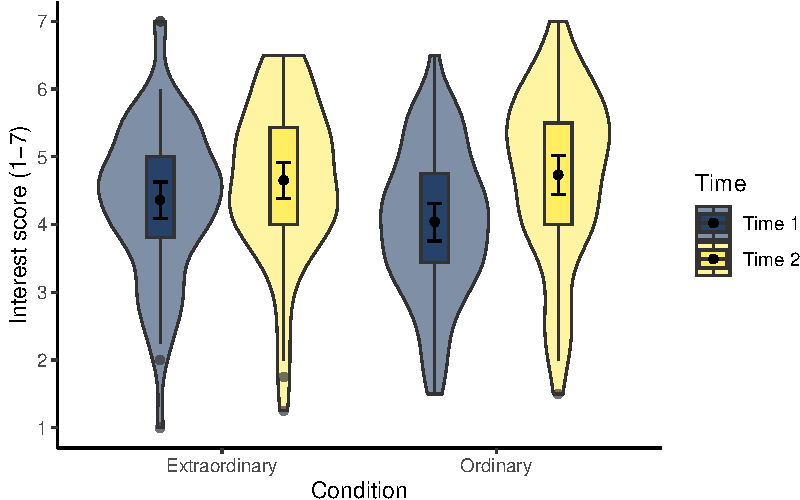
\includegraphics[width=1\textwidth,height=\textheight]{13-factorial-anova_files/figure-pdf/unnamed-chunk-2-1.pdf}
\end{center}

\end{tcolorbox}

\begin{tcolorbox}[enhanced jigsaw, breakable, colframe=quarto-callout-caution-color-frame, arc=.35mm, opacitybacktitle=0.6, titlerule=0mm, colbacktitle=quarto-callout-caution-color!10!white, colback=white, toprule=.15mm, bottomtitle=1mm, toptitle=1mm, title=\textcolor{quarto-callout-caution-color}{\faFire}\hspace{0.5em}{Show me the solution}, bottomrule=.15mm, rightrule=.15mm, leftrule=.75mm, coltitle=black, left=2mm, opacityback=0]

You should have the following in a code chunk:

\begin{Shaded}
\begin{Highlighting}[]
\CommentTok{\# specify as an object, so we only change it in one place}
\NormalTok{dodge\_value }\OtherTok{\textless{}{-}} \FloatTok{0.9}

\NormalTok{zhang\_long }\SpecialCharTok{\%\textgreater{}\%} 
  \FunctionTok{mutate}\NormalTok{(}\AttributeTok{Time =} \FunctionTok{case\_match}\NormalTok{(Time,}
                           \StringTok{"time1\_interest"} \SpecialCharTok{\textasciitilde{}} \StringTok{"Time 1"}\NormalTok{,}
                           \StringTok{"time2\_interest"} \SpecialCharTok{\textasciitilde{}} \StringTok{"Time 2"}\NormalTok{)) }\SpecialCharTok{\%\textgreater{}\%} 
  \FunctionTok{ggplot}\NormalTok{(}\FunctionTok{aes}\NormalTok{(}\AttributeTok{y =}\NormalTok{ Interest, }\AttributeTok{x =}\NormalTok{ Condition, }\AttributeTok{fill =}\NormalTok{ Time)) }\SpecialCharTok{+}
  \FunctionTok{geom\_violin}\NormalTok{(}\AttributeTok{alpha =} \FloatTok{0.5}\NormalTok{) }\SpecialCharTok{+} 
  \FunctionTok{geom\_boxplot}\NormalTok{(}\AttributeTok{width =} \FloatTok{0.2}\NormalTok{, }
               \AttributeTok{alpha =} \FloatTok{0.7}\NormalTok{,}
               \AttributeTok{fatten =} \ConstantTok{NULL}\NormalTok{,}
               \AttributeTok{position =} \FunctionTok{position\_dodge}\NormalTok{(dodge\_value)) }\SpecialCharTok{+} 
  \FunctionTok{stat\_summary}\NormalTok{(}\AttributeTok{fun =} \StringTok{"mean"}\NormalTok{, }
               \AttributeTok{geom =} \StringTok{"point"}\NormalTok{,}
               \AttributeTok{position =} \FunctionTok{position\_dodge}\NormalTok{(dodge\_value)) }\SpecialCharTok{+}
  \FunctionTok{stat\_summary}\NormalTok{(}\AttributeTok{fun.data =} \StringTok{"mean\_cl\_boot"}\NormalTok{, }
               \AttributeTok{geom =} \StringTok{"errorbar"}\NormalTok{, }
               \AttributeTok{width =}\NormalTok{ .}\DecValTok{1}\NormalTok{,}
               \AttributeTok{position =} \FunctionTok{position\_dodge}\NormalTok{(dodge\_value)) }\SpecialCharTok{+}
  \FunctionTok{scale\_fill\_viridis\_d}\NormalTok{(}\AttributeTok{option =} \StringTok{"E"}\NormalTok{) }\SpecialCharTok{+} 
  \FunctionTok{scale\_y\_continuous}\NormalTok{(}\AttributeTok{name =} \StringTok{"Interest score (1{-}7)"}\NormalTok{, }
                     \AttributeTok{breaks =} \FunctionTok{c}\NormalTok{(}\DecValTok{1}\SpecialCharTok{:}\DecValTok{7}\NormalTok{)) }\SpecialCharTok{+} 
  \FunctionTok{theme\_classic}\NormalTok{()}
\end{Highlighting}
\end{Shaded}

\end{tcolorbox}

\section{Factorial ANOVA}\label{factorial-anova}

To run the factorial ANOVA, we will be using the afex package again.
Remember that you must specify both IVs, one of which is
between-subjects and the other is within-subjects. Look up the help
documentation for \texttt{aov\_ez} if you need further information.

\subsection{\texorpdfstring{Activity 4 - Using the \texttt{aov\_ez()}
function.}{Activity 4 - Using the aov\_ez() function.}}\label{activity-4---using-the-aov_ez-function.}

Before we show you the code, try and complete the following skeleton
version first. Think about what variable in the data corresponds to each
argument.

Save the ANOVA model to an object called \texttt{mod\_factorial} to be
consistent with explanations below. For making it easier to report the
results later, pull out the \texttt{mod\_factorial\$anova\_table}
component and apply the \texttt{tidy()} function from broom as a second
step.

\begin{Shaded}
\begin{Highlighting}[]
\NormalTok{mod\_factorial }\OtherTok{\textless{}{-}} \FunctionTok{aov\_ez}\NormalTok{(}\AttributeTok{id =} \StringTok{"NULL"}\NormalTok{,}
               \AttributeTok{data =} \ConstantTok{NULL}\NormalTok{, }
               \AttributeTok{between =} \StringTok{"NULL"}\NormalTok{, }
               \AttributeTok{within =} \StringTok{"NULL"}\NormalTok{,}
               \AttributeTok{dv =} \StringTok{"NULL"}\NormalTok{, }
               \AttributeTok{type =} \DecValTok{3}\NormalTok{,}
               \AttributeTok{anova\_table =} \FunctionTok{list}\NormalTok{(}\AttributeTok{es =} \StringTok{"NULL"}\NormalTok{)) }

\NormalTok{factorial\_output }\OtherTok{\textless{}{-}} \ConstantTok{NULL}
\end{Highlighting}
\end{Shaded}

\begin{tcolorbox}[enhanced jigsaw, breakable, colframe=quarto-callout-caution-color-frame, arc=.35mm, opacitybacktitle=0.6, titlerule=0mm, colbacktitle=quarto-callout-caution-color!10!white, colback=white, toprule=.15mm, bottomtitle=1mm, toptitle=1mm, title=\textcolor{quarto-callout-caution-color}{\faFire}\hspace{0.5em}{Show me the solution}, bottomrule=.15mm, rightrule=.15mm, leftrule=.75mm, coltitle=black, left=2mm, opacityback=0]

You should have the following in a code chunk:

\begin{Shaded}
\begin{Highlighting}[]
\NormalTok{mod\_factorial }\OtherTok{\textless{}{-}} \FunctionTok{aov\_ez}\NormalTok{(}\AttributeTok{id =} \StringTok{"participant\_ID"}\NormalTok{,}
                        \AttributeTok{data =}\NormalTok{ zhang\_long, }
                        \AttributeTok{between =} \StringTok{"Condition"}\NormalTok{, }
                        \AttributeTok{within =} \StringTok{"Time"}\NormalTok{,}
                        \AttributeTok{dv =} \StringTok{"Interest"}\NormalTok{, }
                        \AttributeTok{type =} \DecValTok{3}\NormalTok{,}
                        \AttributeTok{include\_aov =} \ConstantTok{TRUE}\NormalTok{,}
                        \AttributeTok{anova\_table =} \FunctionTok{list}\NormalTok{(}\AttributeTok{es =} \StringTok{"pes"}\NormalTok{)) }

\NormalTok{factorial\_output }\OtherTok{\textless{}{-}}\NormalTok{ mod\_factorial}\SpecialCharTok{$}\NormalTok{anova\_table }\SpecialCharTok{\%\textgreater{}\%} 
  \FunctionTok{tidy}\NormalTok{()}
\end{Highlighting}
\end{Shaded}

We can look at the results of the factorial ANOVA by printing the
object.

\begin{Shaded}
\begin{Highlighting}[]
\NormalTok{mod\_factorial}
\end{Highlighting}
\end{Shaded}

\begin{verbatim}
Anova Table (Type 3 tests)

Response: Interest
          Effect     df  MSE         F  pes p.value
1      Condition 1, 128 2.05      0.46 .004    .498
2           Time 1, 128 0.61 25.88 *** .168   <.001
3 Condition:Time 1, 128 0.61    4.44 * .034    .037
---
Signif. codes:  0 '***' 0.001 '**' 0.01 '*' 0.05 '+' 0.1 ' ' 1
\end{verbatim}

\end{tcolorbox}

Look at the results. Remember the pre-class information about how to
read \emph{p}-values in scientific notation.

\begin{itemize}
\item
  Is the main effect of Condition significant?
\item
  \begin{enumerate}
  \def\labelenumi{(\Alph{enumi})}
  \tightlist
  \item
    Yes\\
  \end{enumerate}
\item
  \begin{enumerate}
  \def\labelenumi{(\Alph{enumi})}
  \setcounter{enumi}{1}
  \tightlist
  \item
    No
  \end{enumerate}
\item
  Is the main effect of Time significant?
\item
  \begin{enumerate}
  \def\labelenumi{(\Alph{enumi})}
  \tightlist
  \item
    Yes\\
  \end{enumerate}
\item
  \begin{enumerate}
  \def\labelenumi{(\Alph{enumi})}
  \setcounter{enumi}{1}
  \tightlist
  \item
    No
  \end{enumerate}
\item
  Is the two-way interaction significant?
\item
  \begin{enumerate}
  \def\labelenumi{(\Alph{enumi})}
  \tightlist
  \item
    Yes\\
  \end{enumerate}
\item
  \begin{enumerate}
  \def\labelenumi{(\Alph{enumi})}
  \setcounter{enumi}{1}
  \tightlist
  \item
    No
  \end{enumerate}
\end{itemize}

\subsection{Activity 5 - Checking assumptions for factorial
ANOVA}\label{factorial-a5}

The assumptions for a factorial ANOVA are the same as the one-way ANOVA.

\begin{enumerate}
\def\labelenumi{\arabic{enumi}.}
\item
  The DV is interval or ratio data.
\item
  The observations should be independent.
\item
  The residuals should be normally distributed.
\item
  There should be homogeneity of variance between the groups.
\end{enumerate}

As before, we know assumption 2 is met from the design of the study.
Assumption 1 throws up an interesting issue which is the problem of
ordinal data. Ordinal data are the kind of data that come from Likert
scales and are very common in psychology. The problem is that ordinal
data are not interval or ratio data, there's a fixed number of integer
values they can take (the values of the Likert scale) and you cannot
claim that the distance between the values is equal (is the difference
between strongly agree and agree the same as the difference between
agree and neutral?).

Technically, we should not use an ANOVA to analyse ordinal data -
\emph{but almost everyone does}. Many people argue that if you take the
average of multiple Likert scale items, you can interpret the data as if
they are interval and they can be normally distributed. Other people
argue you should use non-parametric methods or more complex models such
as ordinal regression for this type of data, but it is beyond the scope
of what we cover in this course (if you are super interested, there is a
PsyTeachR book for another course -
\href{https://psyteachr.github.io/statsres-v2/}{Statistics and Research
Design} - which covers ordinal regression). Whichever route you choose,
you should understand the data you have and you should be able to
justify your decision.

To test assumption 3, you can run \texttt{check\_model()} from
performance on the model object (\texttt{mod\_factorial}). Unless you
add the argument \texttt{re\_formula\ =\ NA}, you get a little warning
saying the function does it anyway. The background of this argument is
beyond the scope of this course, but expressed as a linear model, a
mixed ANOVA looks like something called a mixed-effects model, so this
argument is saying that there is not a formula for it, since we did not
have one.

\begin{Shaded}
\begin{Highlighting}[]
\FunctionTok{check\_model}\NormalTok{(mod\_factorial, }
            \AttributeTok{re\_formula =} \ConstantTok{NA}\NormalTok{) }\CommentTok{\# Specify or you get a warning }
\end{Highlighting}
\end{Shaded}

\begin{center}
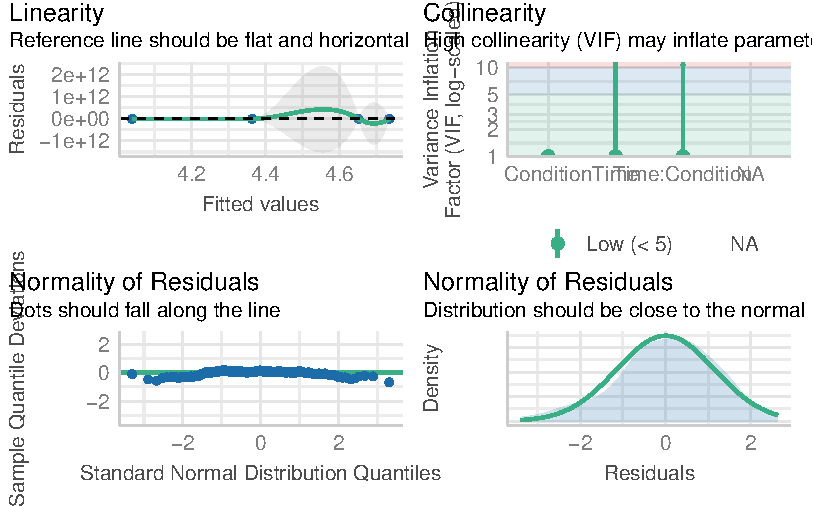
\includegraphics[width=1\textwidth,height=\textheight]{13-factorial-anova_files/figure-pdf/unnamed-chunk-5-1.pdf}
\end{center}

Does it look like we have any obvious problems with normality here?

\begin{itemize}
\tightlist
\item
  \begin{enumerate}
  \def\labelenumi{(\Alph{enumi})}
  \tightlist
  \item
    Yes\\
  \end{enumerate}
\item
  \begin{enumerate}
  \def\labelenumi{(\Alph{enumi})}
  \setcounter{enumi}{1}
  \tightlist
  \item
    No
  \end{enumerate}
\end{itemize}

The one annoying thing here is we do not get a diagnostic plot for
checking homogeneity of variance / homoscedasticity. We can create our
own using the lm component of the model object
(\texttt{mod\_factorial\$lm}), but it takes a few steps. In the code
below:

\begin{itemize}
\item
  We first isolate the standardised residuals of the model object. We
  must convert it to a data frame and rename the two columns.
\item
  We combine the residuals with the wide version of the data.
\item
  We pivot the data longer so all the residuals are in one column and
  create a new variable to take the square root of the absolute
  residuals. This recreates how the diagnostic plots you saw in Chapters
  8, 9, and 12 look.
\item
  Finally, we plot the standardised residuals and add a line to join the
  means of each group. If the line is roughly flat, we support
  homoscedasticity. If the line angles up or down substantially, then
  this points to signs of heteroscedasticity.
\end{itemize}

\begin{Shaded}
\begin{Highlighting}[]
\CommentTok{\# Isolate standardised residuals as a data frame}
\NormalTok{residuals }\OtherTok{\textless{}{-}} \FunctionTok{as.data.frame}\NormalTok{(}\FunctionTok{rstandard}\NormalTok{(mod\_factorial}\SpecialCharTok{$}\NormalTok{lm)) }\SpecialCharTok{\%\textgreater{}\%} 
  \FunctionTok{select}\NormalTok{(}\AttributeTok{residuals\_time1 =}\NormalTok{ time1\_interest,}
         \AttributeTok{residuals\_time2 =}\NormalTok{ time2\_interest)}

\CommentTok{\# add residuals to the wide version of the data, so we have the groups}
\NormalTok{zhang\_wide }\OtherTok{\textless{}{-}}\NormalTok{ zhang\_wide }\SpecialCharTok{\%\textgreater{}\%} 
  \FunctionTok{bind\_cols}\NormalTok{(residuals)}

\CommentTok{\# Pivot longer and calculate the square root of absolute standardised residuals}
\NormalTok{residuals\_long }\OtherTok{\textless{}{-}}\NormalTok{ zhang\_wide }\SpecialCharTok{\%\textgreater{}\%} 
  \FunctionTok{pivot\_longer}\NormalTok{(}\AttributeTok{cols =}\NormalTok{ residuals\_time1}\SpecialCharTok{:}\NormalTok{residuals\_time2, }
               \AttributeTok{names\_to =} \StringTok{"Time"}\NormalTok{, }
               \AttributeTok{values\_to =} \StringTok{"Residuals"}\NormalTok{) }\SpecialCharTok{\%\textgreater{}\%} 
  \FunctionTok{mutate}\NormalTok{(}\AttributeTok{std\_residuals =} \FunctionTok{sqrt}\NormalTok{(}\FunctionTok{abs}\NormalTok{(Residuals)))}

\CommentTok{\# Plot the residuals}
\NormalTok{residuals\_long }\SpecialCharTok{\%\textgreater{}\%}
  \CommentTok{\# we need groups as numbers for the line to plot }
  \FunctionTok{mutate}\NormalTok{(}\AttributeTok{Condition =} \FunctionTok{case\_match}\NormalTok{(Condition,}
                                \StringTok{"Ordinary"} \SpecialCharTok{\textasciitilde{}} \DecValTok{1}\NormalTok{,}
                                \StringTok{"Extraordinary"} \SpecialCharTok{\textasciitilde{}} \DecValTok{2}\NormalTok{)) }\SpecialCharTok{\%\textgreater{}\%} 
  \FunctionTok{ggplot}\NormalTok{(}\FunctionTok{aes}\NormalTok{(}\AttributeTok{x =}\NormalTok{ Condition, }\AttributeTok{y =}\NormalTok{ std\_residuals)) }\SpecialCharTok{+} 
  \FunctionTok{geom\_point}\NormalTok{() }\SpecialCharTok{+} 
  \CommentTok{\# add line joining the mean of residuals per group}
  \FunctionTok{stat\_summary}\NormalTok{(}\AttributeTok{geom =} \StringTok{"line"}\NormalTok{, }
               \AttributeTok{fun =}\NormalTok{ mean, }
               \AttributeTok{color =} \StringTok{"blue"}\NormalTok{, }
               \AttributeTok{linewidth =} \FloatTok{1.5}\NormalTok{) }\SpecialCharTok{+} 
    \FunctionTok{labs}\NormalTok{(}\AttributeTok{x =} \StringTok{"Condition"}\NormalTok{, }\AttributeTok{y =} \StringTok{"Standardised Residuals"}\NormalTok{)}
\end{Highlighting}
\end{Shaded}

\begin{center}
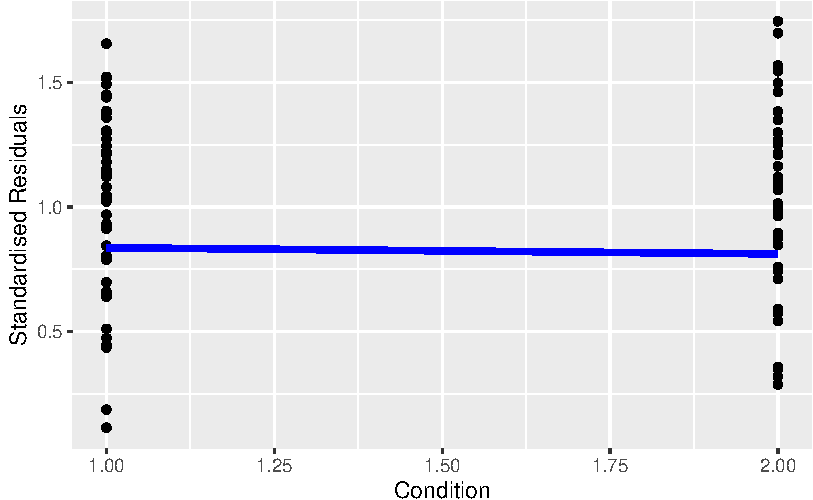
\includegraphics[width=1\textwidth,height=\textheight]{13-factorial-anova_files/figure-pdf/unnamed-chunk-6-1.pdf}
\end{center}

Does it look like we have any obvious problems with homoscedasticity
here?

\begin{itemize}
\tightlist
\item
  \begin{enumerate}
  \def\labelenumi{(\Alph{enumi})}
  \tightlist
  \item
    Yes\\
  \end{enumerate}
\item
  \begin{enumerate}
  \def\labelenumi{(\Alph{enumi})}
  \setcounter{enumi}{1}
  \tightlist
  \item
    No
  \end{enumerate}
\end{itemize}

\subsection{Activity 6 - Post-hoc tests}\label{factorial-a6}

Because the interaction is significant, we should follow this up with
post-hoc tests using \texttt{emmeans()} to determine which comparisons
are significant. If the overall interaction is not significant, you
should not conduct additional tests.

\texttt{emmeans()} requires you to specify the \texttt{aov} object, and
then the factors you want to contrast. For an interaction, we use the
notation \texttt{pairwise\ \textasciitilde{}\ IV1\ \textbar{}\ IV2} and
you specify which multiple comparison correction you want to apply.

Run the below code and view the results.

\begin{Shaded}
\begin{Highlighting}[]
\CommentTok{\# run the tests}
\NormalTok{posthoc\_factorial }\OtherTok{\textless{}{-}} \FunctionTok{emmeans}\NormalTok{(mod\_factorial, }
\NormalTok{                             pairwise }\SpecialCharTok{\textasciitilde{}}\NormalTok{ Time }\SpecialCharTok{|}\NormalTok{ Condition, }
                             \AttributeTok{adjust =} \StringTok{"bonferroni"}\NormalTok{)}

\NormalTok{posthoc\_factorial}
\end{Highlighting}
\end{Shaded}

\begin{verbatim}
$emmeans
Condition = Extraordinary:
 Time           emmean    SE  df lower.CL upper.CL
 time1_interest   4.36 0.137 128     4.09     4.63
 time2_interest   4.65 0.147 128     4.36     4.94

Condition = Ordinary:
 Time           emmean    SE  df lower.CL upper.CL
 time1_interest   4.04 0.139 128     3.76     4.31
 time2_interest   4.73 0.149 128     4.44     5.03

Confidence level used: 0.95 

$contrasts
Condition = Extraordinary:
 contrast                        estimate    SE  df t.ratio p.value
 time1_interest - time2_interest   -0.288 0.136 128  -2.123  0.0357

Condition = Ordinary:
 contrast                        estimate    SE  df t.ratio p.value
 time1_interest - time2_interest   -0.695 0.138 128  -5.049  <.0001
\end{verbatim}

In the output, we first get the estimated marginal means for the
combination of IVs. We then get the contrasts we requested. This looks
at the difference in levels of the first IV for each level of the second
IV.

You can use \texttt{tidy()} to tidy up the output of the contrasts and
save it into a tibble which makes it easier to use in inline code later.

\begin{Shaded}
\begin{Highlighting}[]
\CommentTok{\# tidy up the output of the tests}
\NormalTok{contrasts\_factorial }\OtherTok{\textless{}{-}}\NormalTok{ posthoc\_factorial}\SpecialCharTok{$}\NormalTok{contrasts }\SpecialCharTok{\%\textgreater{}\%}
  \FunctionTok{tidy}\NormalTok{()}

\NormalTok{contrasts\_factorial}
\end{Highlighting}
\end{Shaded}

\begin{verbatim}
# A tibble: 2 x 9
  Condition term  contrast null.value estimate std.error    df statistic p.value
  <chr>     <chr> <chr>         <dbl>    <dbl>     <dbl> <dbl>     <dbl>   <dbl>
1 Extraord~ Time  time1_i~          0   -0.288     0.136   128     -2.12 3.57e-2
2 Ordinary  Time  time1_i~          0   -0.695     0.138   128     -5.05 1.49e-6
\end{verbatim}

Note that because there are two IVs/factors, we could also reverse the
order. Above, we get the results contrasting time 1 and time 2 for each
event condition. Instead, we could look at the difference between
ordinary and extraordinary events at each time point.

Run the code below and compare the output to
\texttt{contrast\_factorial}. Look at how the contrasts are expressed
subtly different when you switch the order. Think carefully about your
research question and hypotheses for which way around is the most
informative.

\begin{Shaded}
\begin{Highlighting}[]
\NormalTok{posthoc\_factorial2 }\OtherTok{\textless{}{-}} \FunctionTok{emmeans}\NormalTok{(mod\_factorial, }
\NormalTok{                             pairwise }\SpecialCharTok{\textasciitilde{}}\NormalTok{ Condition }\SpecialCharTok{|}\NormalTok{ Time, }
                             \AttributeTok{adjust =} \StringTok{"bonferroni"}\NormalTok{) }

\NormalTok{posthoc\_factorial2}

\NormalTok{contrasts\_factorial2 }\OtherTok{\textless{}{-}}\NormalTok{ posthoc\_factorial2}\SpecialCharTok{$}\NormalTok{contrasts }\SpecialCharTok{\%\textgreater{}\%}
  \FunctionTok{tidy}\NormalTok{()}

\NormalTok{contrasts\_factorial2}
\end{Highlighting}
\end{Shaded}

\begin{verbatim}
$emmeans
Time = time1_interest:
 Condition     emmean    SE  df lower.CL upper.CL
 Extraordinary   4.36 0.137 128     4.09     4.63
 Ordinary        4.04 0.139 128     3.76     4.31

Time = time2_interest:
 Condition     emmean    SE  df lower.CL upper.CL
 Extraordinary   4.65 0.147 128     4.36     4.94
 Ordinary        4.73 0.149 128     4.44     5.03

Confidence level used: 0.95 

$contrasts
Time = time1_interest:
 contrast                 estimate    SE  df t.ratio p.value
 Extraordinary - Ordinary   0.3246 0.195 128   1.661  0.0992

Time = time2_interest:
 contrast                 estimate    SE  df t.ratio p.value
 Extraordinary - Ordinary  -0.0829 0.209 128  -0.397  0.6923


# A tibble: 2 x 9
  Time      term  contrast null.value estimate std.error    df statistic p.value
  <chr>     <chr> <chr>         <dbl>    <dbl>     <dbl> <dbl>     <dbl>   <dbl>
1 time1_in~ Cond~ Extraor~          0   0.325      0.195   128     1.66   0.0992
2 time2_in~ Cond~ Extraor~          0  -0.0829     0.209   128    -0.397  0.692 
\end{verbatim}

Because our main effects (condition and time) only have two levels, we
do not need to do any post-hoc tests to determine which conditions
differ from each other, however, if one of our factors had three levels
then we could use \texttt{emmeans()} to calculate the contrast for the
main effects, like we did for the one-way ANOVA.

Finally, to calculate standardised effect sizes for the pairwise
comparisons, we again need to do this individually using
\texttt{cohens\_d()} from effectsize.

As we have a mixed design, we must follow a slightly different process
for each comparison. Cohen's d has a different calculation for
between-subjects and within-subjects contrasts, so we must express it
differently. For the first comparison, we are interested in the
difference between time 1 and time 2 for each group, so this represents
a within-subjects comparison.

\begin{Shaded}
\begin{Highlighting}[]
\CommentTok{\# time 1 vs time 2 for Extraordinary group}
\NormalTok{d\_extraordinary }\OtherTok{\textless{}{-}} \FunctionTok{cohens\_d}\NormalTok{(}\AttributeTok{x =} \StringTok{"time1\_interest"}\NormalTok{, }
                            \AttributeTok{y =} \StringTok{"time2\_interest"}\NormalTok{, }
                            \AttributeTok{paired =} \ConstantTok{TRUE}\NormalTok{,}
                            \AttributeTok{data =} \FunctionTok{filter}\NormalTok{(zhang\_wide, }
\NormalTok{                                          Condition }\SpecialCharTok{==} \StringTok{"Extraordinary"}\NormalTok{))}
\CommentTok{\# time 1 vs time 2 for Ordinary group}
\NormalTok{d\_ordinary }\OtherTok{\textless{}{-}} \FunctionTok{cohens\_d}\NormalTok{(}\AttributeTok{x =} \StringTok{"time1\_interest"}\NormalTok{, }
                       \AttributeTok{y =} \StringTok{"time2\_interest"}\NormalTok{, }
                       \AttributeTok{paired =} \ConstantTok{TRUE}\NormalTok{,}
                       \AttributeTok{data =} \FunctionTok{filter}\NormalTok{(zhang\_wide, }
\NormalTok{                                     Condition }\SpecialCharTok{==} \StringTok{"Ordinary"}\NormalTok{))}

\CommentTok{\# bind together the two contrasts}
\NormalTok{Condition\_ds }\OtherTok{\textless{}{-}} \FunctionTok{bind\_rows}\NormalTok{(d\_extraordinary, }
\NormalTok{                          d\_ordinary)}

\CommentTok{\# add the contrasts to the emmeans tidy table}
\NormalTok{contrasts\_factorial }\OtherTok{\textless{}{-}}\NormalTok{ contrasts\_factorial }\SpecialCharTok{\%\textgreater{}\%}
  \FunctionTok{bind\_cols}\NormalTok{(Condition\_ds)}

\NormalTok{contrasts\_factorial}
\end{Highlighting}
\end{Shaded}

\begin{verbatim}
# A tibble: 2 x 13
  Condition term  contrast null.value estimate std.error    df statistic p.value
  <chr>     <chr> <chr>         <dbl>    <dbl>     <dbl> <dbl>     <dbl>   <dbl>
1 Extraord~ Time  time1_i~          0   -0.288     0.136   128     -2.12 3.57e-2
2 Ordinary  Time  time1_i~          0   -0.695     0.138   128     -5.05 1.49e-6
# i 4 more variables: Cohens_d <dbl>, CI <dbl>, CI_low <dbl>, CI_high <dbl>
\end{verbatim}

For the second comparison, we are interested in the difference between
ordinary and extraordinary at each time point, so this represents a
between-subjects comparison.

\begin{Shaded}
\begin{Highlighting}[]
\CommentTok{\# Extraordinary vs ordinary at time 1}
\NormalTok{d\_time1 }\OtherTok{\textless{}{-}} \FunctionTok{cohens\_d}\NormalTok{(time1\_interest }\SpecialCharTok{\textasciitilde{}}\NormalTok{ Condition,}
                       \AttributeTok{data =}\NormalTok{ zhang\_wide)}

\CommentTok{\# Extraordinary vs ordinary at time 2}
\NormalTok{d\_time2 }\OtherTok{\textless{}{-}} \FunctionTok{cohens\_d}\NormalTok{(time2\_interest }\SpecialCharTok{\textasciitilde{}}\NormalTok{ Condition,}
                       \AttributeTok{data =}\NormalTok{ zhang\_wide)}

\CommentTok{\# bind the two contrasts together}
\NormalTok{Time\_ds }\OtherTok{\textless{}{-}} \FunctionTok{bind\_rows}\NormalTok{(d\_time1,}
\NormalTok{                     d\_time2)}

\CommentTok{\# add the contrasts to the emmeans tidy table}
\NormalTok{contrasts\_factorial2 }\OtherTok{\textless{}{-}}\NormalTok{ contrasts\_factorial2 }\SpecialCharTok{\%\textgreater{}\%}
  \FunctionTok{bind\_cols}\NormalTok{(Time\_ds)}

\NormalTok{contrasts\_factorial2}
\end{Highlighting}
\end{Shaded}

\begin{verbatim}
# A tibble: 2 x 13
  Time      term  contrast null.value estimate std.error    df statistic p.value
  <chr>     <chr> <chr>         <dbl>    <dbl>     <dbl> <dbl>     <dbl>   <dbl>
1 time1_in~ Cond~ Extraor~          0   0.325      0.195   128     1.66   0.0992
2 time2_in~ Cond~ Extraor~          0  -0.0829     0.209   128    -0.397  0.692 
# i 4 more variables: Cohens_d <dbl>, CI <dbl>, CI_low <dbl>, CI_high <dbl>
\end{verbatim}

\subsection{Activity 7 - Creating an interaction
plot}\label{factorial-a7}

When you have a factorial design, one powerful way of visualising the
data is through an interaction plot. This is essentially a line graph
where the x-axis has one IV and separate lines for a second IV. However,
once you have the factorial ANOVA model, you can add confidence
intervals to the plot to visualise uncertainty. afex has it's own
function called \texttt{afex\_plot()} which you can use with the model
object you created.

In the code below, there are a few key argument to highlight:

\begin{itemize}
\item
  \texttt{object} is the afex model you created.
\item
  \texttt{x} is the variable you want on the x-axis.
\item
  \texttt{trace} is the variable you want to plot as separate lines.
\item
  \texttt{error} controls whether the error bars show confidence
  intervals for between-subjects or within-subjects. In a mixed design,
  these have different properties, so you must think about which you
  want to plot and highlight to the reader.
\item
  \texttt{factor\_levels} lets you edit the levels of factors you plot,
  such as renaming or reordering them. You add each factor into a list
  but check the documentation and vignettes for other options.
\end{itemize}

\begin{Shaded}
\begin{Highlighting}[]
\FunctionTok{afex\_plot}\NormalTok{(}\AttributeTok{object =}\NormalTok{ mod\_factorial, }
          \AttributeTok{x =} \StringTok{"Condition"}\NormalTok{, }
          \AttributeTok{trace =} \StringTok{"Time"}\NormalTok{, }
          \AttributeTok{error =} \StringTok{"between"}\NormalTok{,}
          \AttributeTok{factor\_levels =} \FunctionTok{list}\NormalTok{(}\AttributeTok{Time =} \FunctionTok{c}\NormalTok{(}\StringTok{"Time 1"}\NormalTok{, }\StringTok{"Time 2"}\NormalTok{)))}
\end{Highlighting}
\end{Shaded}

\begin{center}
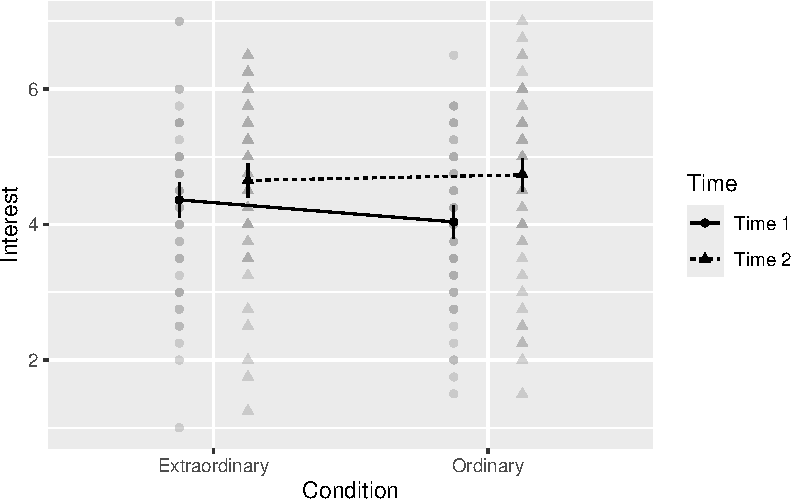
\includegraphics[width=1\textwidth,height=\textheight]{13-factorial-anova_files/figure-pdf/unnamed-chunk-10-1.pdf}
\end{center}

One handy feature about this function is it uses ggplot2 in the
background, so you can add layers to the initial function like other
plots that you have created.

\begin{Shaded}
\begin{Highlighting}[]
\FunctionTok{afex\_plot}\NormalTok{(mod\_factorial, }
          \AttributeTok{x =} \StringTok{"Condition"}\NormalTok{, }
          \AttributeTok{trace =} \StringTok{"Time"}\NormalTok{, }
          \AttributeTok{error =} \StringTok{"between"}\NormalTok{,}
          \AttributeTok{factor\_levels =} \FunctionTok{list}\NormalTok{(}\AttributeTok{Time =} \FunctionTok{c}\NormalTok{(}\StringTok{"Time 1"}\NormalTok{, }\StringTok{"Time 2"}\NormalTok{))) }\SpecialCharTok{+} 
  \FunctionTok{theme\_classic}\NormalTok{() }\SpecialCharTok{+} 
  \FunctionTok{scale\_y\_continuous}\NormalTok{(}\AttributeTok{breaks =} \DecValTok{1}\SpecialCharTok{:}\DecValTok{7}\NormalTok{)}
\end{Highlighting}
\end{Shaded}

\begin{center}
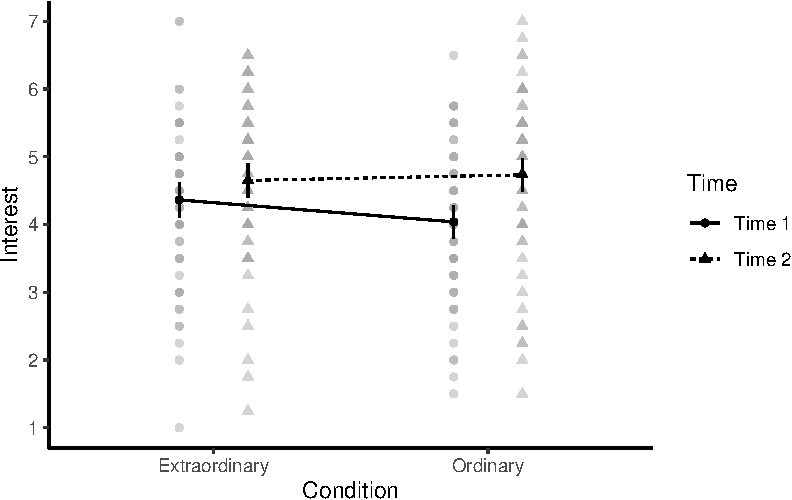
\includegraphics[width=1\textwidth,height=\textheight]{13-factorial-anova_files/figure-pdf/unnamed-chunk-11-1.pdf}
\end{center}

\begin{tcolorbox}[enhanced jigsaw, breakable, colframe=quarto-callout-note-color-frame, arc=.35mm, opacitybacktitle=0.6, titlerule=0mm, colbacktitle=quarto-callout-note-color!10!white, colback=white, toprule=.15mm, bottomtitle=1mm, toptitle=1mm, title=\textcolor{quarto-callout-note-color}{\faInfo}\hspace{0.5em}{Note}, bottomrule=.15mm, rightrule=.15mm, leftrule=.75mm, coltitle=black, left=2mm, opacityback=0]

Since \texttt{afex\_plot()} uses ggplot2, you can use \texttt{ggsave()}
to save your plots and insert them into your work.

\end{tcolorbox}

\section{Reporting the results of your factorial
ANOVA}\label{factorial-a8}

Now you have all your values, we can work on the write-up of your
results.

In the in-line code demonstration below, we manually entered
\emph{p}-values where they are \textless{} .001. There is a way to get R
to produce this formatting but it's overly complicated for our purposes
in this course. If you want to push yourself, look up the
\href{https://github.com/crsh/papaja}{papaja} package for creating
reproducible manuscripts.

The values of partial eta-squared do not match between our analysis and
those reported in the paper. We have not figured out why this is yet, so
if you know, please get in touch!

We have also replaced the simple effects in the main paper with our
pairwise comparisons.

Copy and paste the text and inline code below into \textbf{white-space}
in your R Markdown document. If you saved all the descriptives, model,
and contrasts using the same object names as us, this should knit.

\begin{Shaded}
\begin{Highlighting}[]
\NormalTok{We conducted the same repeated measures ANOVA with interest as the dependent measure and again found a main effect of time, }\FunctionTok{F}\NormalTok{(}\StringTok{\textasciigrave{}}\AttributeTok{r factorial\_output$num.Df[2]}\StringTok{\textasciigrave{}}\NormalTok{, }\StringTok{\textasciigrave{}}\AttributeTok{r factorial\_output$den.Df[2]}\StringTok{\textasciigrave{}}\NormalTok{) }\OtherTok{=} \StringTok{\textasciigrave{}}\AttributeTok{r factorial\_output$statistic[2] \%\textgreater{}\% round(2)}\StringTok{\textasciigrave{}}\NormalTok{, p }\SpecialCharTok{\textless{}}\NormalTok{ .}\DecValTok{001}\NormalTok{, ηp2 }\OtherTok{=} \StringTok{\textasciigrave{}}\AttributeTok{r factorial\_output$pes[2] \%\textgreater{}\% round(3)}\StringTok{\textasciigrave{}}\NormalTok{; anticipated interest at Time }\DecValTok{1}\NormalTok{ (}\AttributeTok{M =} \StringTok{\textasciigrave{}}\AttributeTok{r zhang\_descriptives$mean[1] \%\textgreater{}\% round(2)}\StringTok{\textasciigrave{}}\NormalTok{), SD }\OtherTok{=} \StringTok{\textasciigrave{}}\AttributeTok{r zhang\_descriptives$sd[1]\%\textgreater{}\% round(2)}\StringTok{\textasciigrave{}}\ErrorTok{))}\NormalTok{ was lower than actual interest at Time }\DecValTok{2}\NormalTok{ (}\AttributeTok{M =} \StringTok{\textasciigrave{}}\AttributeTok{r zhang\_descriptives$mean[2]\%\textgreater{}\% round(2)}\StringTok{\textasciigrave{}}\NormalTok{, }\AttributeTok{SD =} \StringTok{\textasciigrave{}}\AttributeTok{r zhang\_descriptives$sd[2]\%\textgreater{}\% round(2)}\StringTok{\textasciigrave{}}\NormalTok{). We also observed an interaction between time and type of experience, }\FunctionTok{F}\NormalTok{(}\StringTok{\textasciigrave{}}\AttributeTok{r factorial\_output$num.Df[3]}\StringTok{\textasciigrave{}}\NormalTok{, }\StringTok{\textasciigrave{}}\AttributeTok{r factorial\_output$den.Df[3]}\StringTok{\textasciigrave{}}\NormalTok{) }\OtherTok{=} \StringTok{\textasciigrave{}}\AttributeTok{r factorial\_output$statistic[3] \%\textgreater{}\% round(3)}\StringTok{\textasciigrave{}}\NormalTok{, p }\OtherTok{=} \StringTok{\textasciigrave{}}\AttributeTok{r factorial\_output$p.value[3] \%\textgreater{}\% round(2)}\StringTok{\textasciigrave{}}\NormalTok{, ηp2 }\OtherTok{=} \StringTok{\textasciigrave{}}\AttributeTok{r factorial\_output$pes[3] \%\textgreater{}\% round(3)}\StringTok{\textasciigrave{}}\NormalTok{. Pairwise comparisons revealed that }\ControlFlowTok{for}\NormalTok{ ordinary events, predicted interest at Time }\DecValTok{1}\NormalTok{ (}\AttributeTok{M =} \StringTok{\textasciigrave{}}\AttributeTok{r zhang\_descriptives$mean[3]\%\textgreater{}\% round(2)}\StringTok{\textasciigrave{}}\NormalTok{, }\AttributeTok{SD =} \StringTok{\textasciigrave{}}\AttributeTok{r zhang\_descriptives$sd[3]\%\textgreater{}\% round(2)}\StringTok{\textasciigrave{}}\NormalTok{) was lower than experienced interest at Time }\DecValTok{2}\NormalTok{ (}\AttributeTok{M =} \StringTok{\textasciigrave{}}\AttributeTok{r zhang\_descriptives$mean[4]\%\textgreater{}\% round(2)}\StringTok{\textasciigrave{}}\NormalTok{, }\AttributeTok{SD =} \StringTok{\textasciigrave{}}\AttributeTok{r zhang\_descriptives$sd[4]\%\textgreater{}\% round(2)}\StringTok{\textasciigrave{}}\NormalTok{), }\FunctionTok{t}\NormalTok{(}\StringTok{\textasciigrave{}}\AttributeTok{r contrasts\_factorial$df[2]\%\textgreater{}\% round(2)}\StringTok{\textasciigrave{}}\NormalTok{) }\OtherTok{=} \StringTok{\textasciigrave{}}\AttributeTok{r contrasts\_factorial$statistic[2]\%\textgreater{}\% round(2)}\StringTok{\textasciigrave{}}\NormalTok{, p }\SpecialCharTok{\textless{}}\NormalTok{ .}\DecValTok{001}\NormalTok{, d }\OtherTok{=} \StringTok{\textasciigrave{}}\AttributeTok{r contrasts\_factorial$Cohens\_d[2]\%\textgreater{}\% round(2)}\StringTok{\textasciigrave{}}\NormalTok{. Although predicted interest }\ControlFlowTok{for}\NormalTok{ extraordinary events at Time }\DecValTok{1}\NormalTok{ (}\AttributeTok{M =} \StringTok{\textasciigrave{}}\AttributeTok{r zhang\_descriptives$mean[1]\%\textgreater{}\% round(2)}\StringTok{\textasciigrave{}}\NormalTok{, }\AttributeTok{SD =} \StringTok{\textasciigrave{}}\AttributeTok{r zhang\_descriptives$sd[1]\%\textgreater{}\% round(2)}\StringTok{\textasciigrave{}}\NormalTok{) was lower than experienced interest at Time }\DecValTok{2}\NormalTok{ (}\AttributeTok{M =} \StringTok{\textasciigrave{}}\AttributeTok{r zhang\_descriptives$mean[2]\%\textgreater{}\% round(2)}\StringTok{\textasciigrave{}}\NormalTok{, }\AttributeTok{SD =} \StringTok{\textasciigrave{}}\AttributeTok{r zhang\_descriptives$sd[2]\%\textgreater{}\% round(2)}\StringTok{\textasciigrave{}}\NormalTok{), }\FunctionTok{t}\NormalTok{(}\StringTok{\textasciigrave{}}\AttributeTok{r contrasts\_factorial$df[1]\%\textgreater{}\% round(2)}\StringTok{\textasciigrave{}}\NormalTok{) }\OtherTok{=} \StringTok{\textasciigrave{}}\AttributeTok{r contrasts\_factorial$statistic[1]\%\textgreater{}\% round(2)}\StringTok{\textasciigrave{}}\NormalTok{, p }\SpecialCharTok{\textless{}}\NormalTok{ .}\DecValTok{001}\NormalTok{, d }\OtherTok{=} \StringTok{\textasciigrave{}}\AttributeTok{r contrasts\_factorial$Cohens\_d[1]\%\textgreater{}\% round(2)}\StringTok{\textasciigrave{}}\NormalTok{, the magnitude of underestimation was smaller than }\ControlFlowTok{for}\NormalTok{ ordinary events.}
\end{Highlighting}
\end{Shaded}

\begin{quote}
We conducted the same repeated measures ANOVA with interest as the
dependent measure and again found a main effect of time, F(1, 128) =
25.88, p \textless{} .001, ηp2 = 0.168; anticipated interest at Time 1
(M = 4.36), SD = 1.13)) was lower than actual interest at Time 2 (M =
4.65, SD = 1.14). We also observed an interaction between time and type
of experience, F(1, 128) = 4.445, p = 0.04, ηp2 = 0.034. Pairwise
comparisons revealed that for ordinary events, predicted interest at
Time 1 (M = 4.04, SD = 1.09) was lower than experienced interest at Time
2 (M = 4.73, SD = 1.24), t(128) = -5.05, p \textless{} .001, d = -0.56.
Although predicted interest for extraordinary events at Time 1 (M =
4.36, SD = 1.13) was lower than experienced interest at Time 2 (M =
4.65, SD = 1.14), t(128) = -2.12, p \textless{} .001, d = -0.31, the
magnitude of underestimation was smaller than for ordinary events.
\end{quote}

\section{End of Chapter}\label{end-of-chapter-12}

Well done, you have now covered the ANOVA section of the course to learn
how to express experimental designs into statistical models. ANOVA and
factorial ANOVA are incredibly flexible tools where you can start to
combine multiple independent variables. You might have between-subject
factors, within-subject factors, or a combination of the two in a mixed
design. The most important thing to keep in mind is your research
question, hypothesis, and design come first. Factorial ANOVA can get
arbitrarily more complicated but try and avoid the temptation to create
complex models just because you can. You do not get extra points for
complication, it is better to think about which model will let you
address your research question.

In the next chapter, we finish the core chapters on the final extension
of the general linear model we cover in this course. In Research Methods
1, you learnt about simple linear regression when you only have one
predictor. In multiple linear regression, you can add two or more
predictors, and even the interaction between predictors.

\bookmarksetup{startatroot}

\chapter{Multiple Regression}\label{multiple-regression}

In Chapters 8 and 9 from the Research Methods 1 content, we covered
simple linear regression to investigate the effect of one predictor on
one outcome. At the start of Research Methods 2, we then started to
explore ANOVA models to handle more complex designs.

In this chapter, we end the core content on learning how to apply and
interpret multiple regression models. This uses the full flexibility of
the general linear model to express more complicated designs where you
have multiple predictors or interactions between predictors.

\textbf{Chapter Intended Learning Outcomes (ILOs)}

By the end of this chapter, you will be able to:

\begin{itemize}
\item
  Apply and interpret multiple linear regression models.
\item
  Interpret coefficients from individual predictors and interactions.
\item
  Visualise interactions as model predictions to understand and
  communicate your findings.
\item
  Calculate statistical power for a multiple regression model.
\end{itemize}

\section{Chapter preparation}\label{chapter-preparation-11}

\subsection{Introduction to the data
set}\label{introduction-to-the-data-set-9}

For this chapter, we are using open data from Przybylski \& Weinstein
(2017). The abstract of their article is:

\begin{quote}
Although the time adolescents spend with digital technologies has
sparked widespread concerns that their use might be negatively
associated with mental well-being, these potential deleterious
influences have not been rigorously studied. Using a preregistered plan
for analyzing data collected from a representative sample of English
adolescents (n = 120,115), we obtained evidence that the links between
digital-screen time and mental well-being are described by quadratic
functions. Further, our results showed that these links vary as a
function of when digital technologies are used (i.e., weekday
vs.~weekend), suggesting that a full understanding of the impact of
these recreational activities will require examining their functionality
among other daily pursuits. Overall, the evidence indicated that
moderate use of digital technology is not intrinsically harmful and may
be advantageous in a connected world. The findings inform
recommendations for limiting adolescents' technology use and provide a
template for conducting rigorous investigations into the relations
between digital technology and children's and adolescents' health.
\end{quote}

In summary, this was a large-scale study that found support for the
``Goldilocks'' hypothesis among adolescents: that there is a ``just
right'' amount of screen time, such that any amount more or less than
this amount is associated with lower well-being. This was a huge survey
study: the data contain responses from over 120,000 participants! In
this chapter, we will look at whether the relationship between screen
time and well-being is moderated by participants' (self-reported)
gender.

The outcome/dependant variable used in the study was the
\href{https://warwick.ac.uk/fac/med/research/platform/wemwbs/}{Warwick-Edinburgh
Mental Well-Being Scale (WEMWBS)}. This is a 14-item scale with 5
response categories, summed together to form a single score ranging from
14-70.

Przybylski \& Weinstein (2017) looked at multiple measures of screen
time, but we will be focusing on smartphone use. They found that
decrements in well-being started to appear when respondents reported
more than one hour of weekly smartphone use. Our research question is:
Does the negative association between hours of use and well-being
(beyond the one-hour point) differ for boys and girls?

\subsection{Organising your files and project for the
chapter}\label{organising-your-files-and-project-for-the-chapter-11}

Before we can get started, you need to organise your files and project
for the chapter, so your working directory is in order.

\begin{enumerate}
\def\labelenumi{\arabic{enumi}.}
\item
  In your folder for research methods and the book
  \texttt{ResearchMethods1\_2/Quant\_Fundamentals}, create a new folder
  called \texttt{Chapter\_14\_multiple\_regression}. Within
  \texttt{Chapter\_14\_multiple\_regression}, create two new folders
  called \texttt{data} and \texttt{figures}.
\item
  Create an R Project for \texttt{Chapter\_14\_multiple\_regression} as
  an existing directory for your chapter folder. This should now be your
  working directory.
\item
  Create a new R Markdown document and give it a sensible title
  describing the chapter, such as \texttt{14\ Multiple\ Regression}.
  Delete everything below line 10 so you have a blank file to work with
  and save the file in your \texttt{Chapter\_14\_multiple\_regression}
  folder.
\item
  For this chapter, there are three data files you need. Please save the
  following files:

  \begin{itemize}
  \item
    \href{data/Przybylski_2017_participants.csv}{Przybylski\_2017\_participants.csv}.
  \item
    \href{data/Przybylski_2017_screentime.csv}{Przybylski\_2017\_screentime.csv}
  \item
    \href{data/Przybylski_2017_wellbeing.csv}{Przybylski\_2017\_wellbeing.csv}
  \end{itemize}
\end{enumerate}

Right click the link and select ``save link as'', or clicking the link
will save the files to your Downloads. Make sure that you save the files
as ``.csv''. Save or copy the files to your \texttt{data/} folder within
\texttt{Chapter\_14\_multiple\_regression}.

You are now ready to start working on the chapter!

\subsection{Activity 1 - Load the packages and read the
data}\label{mulregression-a1}

As the first activity, try and test yourself by completing the following
task list.

\begin{tcolorbox}[enhanced jigsaw, breakable, colframe=quarto-callout-tip-color-frame, arc=.35mm, opacitybacktitle=0.6, titlerule=0mm, colbacktitle=quarto-callout-tip-color!10!white, colback=white, toprule=.15mm, bottomtitle=1mm, toptitle=1mm, title=\textcolor{quarto-callout-tip-color}{\faLightbulb}\hspace{0.5em}{Try this}, bottomrule=.15mm, rightrule=.15mm, leftrule=.75mm, coltitle=black, left=2mm, opacityback=0]

To prepare for wrangling the data, complete the following tasks:

\begin{enumerate}
\def\labelenumi{\arabic{enumi}.}
\item
  Load the following packages (one of these is new, so revisit
  \hyperref[install-tidy]{Chapter 1} if you need a refresher of
  installing R packages, but remember not to install packages on the
  university computers / online server):

  \begin{itemize}
  \item
    pwr
  \item
    sjPlot
  \item
    performance
  \item
    tidyverse
  \end{itemize}
\item
  Read the three data files to the following object names to be
  consistent with the tasks below.
\end{enumerate}

\begin{Shaded}
\begin{Highlighting}[]
\CommentTok{\# load packages here}
\NormalTok{?}

\CommentTok{\# read the three data files }
\CommentTok{\# this should be Przybylski\_2017\_participants.csv}
\NormalTok{pinfo }\OtherTok{\textless{}{-}}\NormalTok{ ?}

\CommentTok{\# this should be Przybylski\_2017\_wellbeing.csv}
\NormalTok{wellbeing }\OtherTok{\textless{}{-}}\NormalTok{ ?}

\CommentTok{\# this should be Przybylski\_2017\_screentime.csv}
\NormalTok{screen }\OtherTok{\textless{}{-}}\NormalTok{ ?}
\end{Highlighting}
\end{Shaded}

\end{tcolorbox}

\begin{tcolorbox}[enhanced jigsaw, breakable, colframe=quarto-callout-caution-color-frame, arc=.35mm, opacitybacktitle=0.6, titlerule=0mm, colbacktitle=quarto-callout-caution-color!10!white, colback=white, toprule=.15mm, bottomtitle=1mm, toptitle=1mm, title=\textcolor{quarto-callout-caution-color}{\faFire}\hspace{0.5em}{Show me the solution}, bottomrule=.15mm, rightrule=.15mm, leftrule=.75mm, coltitle=black, left=2mm, opacityback=0]

You should have the following in a code chunk:

\begin{Shaded}
\begin{Highlighting}[]
\CommentTok{\# load packages here}
\FunctionTok{library}\NormalTok{(pwr)}
\FunctionTok{library}\NormalTok{(sjPlot)}
\FunctionTok{library}\NormalTok{(performance)}
\FunctionTok{library}\NormalTok{(tidyverse)}

\CommentTok{\# read the three data files }
\CommentTok{\# this should be Przybylski\_2017\_participants.csv}
\NormalTok{pinfo }\OtherTok{\textless{}{-}} \FunctionTok{read\_csv}\NormalTok{(}\StringTok{"data/Przybylski\_2017\_participants.csv"}\NormalTok{)}

\CommentTok{\# this should be Przybylski\_2017\_wellbeing.csv}
\NormalTok{wellbeing }\OtherTok{\textless{}{-}} \FunctionTok{read\_csv}\NormalTok{(}\StringTok{"data/Przybylski\_2017\_wellbeing.csv"}\NormalTok{)}

\CommentTok{\# this should be Przybylski\_2017\_screentime.csv}
\NormalTok{screen }\OtherTok{\textless{}{-}} \FunctionTok{read\_csv}\NormalTok{(}\StringTok{"data/Przybylski\_2017\_screentime.csv"}\NormalTok{)}
\end{Highlighting}
\end{Shaded}

\end{tcolorbox}

\subsection{Activity 2 - Explore the data}\label{mulregression-a2}

Take a look at the resulting tibbles \texttt{pinfo}, \texttt{wellbeing},
and \texttt{screen}. Use functions like \texttt{glimpse()} to look at
what the data frames contain.

\begin{itemize}
\item
  The \texttt{pinfo} data has information on the participant's
  background.
\item
  The \texttt{wellbeing} data has information from the well-being
  questionnaire.
\item
  The \texttt{screen} data has information about screen time use on
  weekends (variables ending with \texttt{we}) and weekdays (variables
  ending with \texttt{wk}) for four types of activities:

  \begin{itemize}
  \item
    Using a computer (variables starting with \texttt{Comph}; Q10 on the
    survey)
  \item
    Playing video games (variables starting with \texttt{Comp}; Q9 on
    the survey)
  \item
    Using a smartphone (variables starting with \texttt{Smart}; Q11 on
    the survey)
  \item
    Watching TV (variables starting with \texttt{Watch}; Q8 on the
    survey).
  \end{itemize}
\end{itemize}

If you want more information about these variables, look at the items
8-11 on pages 4-5 of the the \href{https://osf.io/82ybd/}{PDF version of
the survey on the authors' OSF project}.

Once you have explored the objects, try and answer the following
questions:

\begin{itemize}
\item
  The variable corresponding to \textbf{gender} is located in the object
  named
\item
  \begin{enumerate}
  \def\labelenumi{(\Alph{enumi})}
  \tightlist
  \item
    pinfo\\
  \end{enumerate}
\item
  \begin{enumerate}
  \def\labelenumi{(\Alph{enumi})}
  \setcounter{enumi}{1}
  \tightlist
  \item
    wellbeing\\
  \end{enumerate}
\item
  \begin{enumerate}
  \def\labelenumi{(\Alph{enumi})}
  \setcounter{enumi}{2}
  \tightlist
  \item
    screen
  \end{enumerate}
\end{itemize}

and this variable is called \_\_\_\_\_\_.

\begin{itemize}
\item
  The well-being data is in
\item
  \begin{enumerate}
  \def\labelenumi{(\Alph{enumi})}
  \tightlist
  \item
    long\\
  \end{enumerate}
\item
  \begin{enumerate}
  \def\labelenumi{(\Alph{enumi})}
  \setcounter{enumi}{1}
  \tightlist
  \item
    wide
  \end{enumerate}
\end{itemize}

format and contains observations from \_\_\_\_\_\_\_\_\_\_ participants
on \_\_ items.

\begin{itemize}
\item
  Individual participants in this data set are identified by the
  variable called \_\_\_\_\_\_\_\_\_. This variable will allow us to
  link information across the three tables.
\item
  If you run the function \texttt{summary()} on the three data sets, are
  there any missing data points?
\item
  \begin{enumerate}
  \def\labelenumi{(\Alph{enumi})}
  \tightlist
  \item
    Yes\\
  \end{enumerate}
\item
  \begin{enumerate}
  \def\labelenumi{(\Alph{enumi})}
  \setcounter{enumi}{1}
  \tightlist
  \item
    No
  \end{enumerate}
\end{itemize}

\subsection{Activity 3 - Compute the well-being score for each
respondent}\label{mulregression-a3}

\begin{tcolorbox}[enhanced jigsaw, breakable, colframe=quarto-callout-tip-color-frame, arc=.35mm, opacitybacktitle=0.6, titlerule=0mm, colbacktitle=quarto-callout-tip-color!10!white, colback=white, toprule=.15mm, bottomtitle=1mm, toptitle=1mm, title=\textcolor{quarto-callout-tip-color}{\faLightbulb}\hspace{0.5em}{Try this}, bottomrule=.15mm, rightrule=.15mm, leftrule=.75mm, coltitle=black, left=2mm, opacityback=0]

The WEMWBS well-being score is simply the \textbf{sum} of all the items.

Wrangle the data to create a new table called \texttt{wemwbs}. The data
should have two variables:

\begin{itemize}
\item
  \texttt{Serial} - the participant ID.
\item
  \texttt{total\_wellbeing} - the total WEMWBS score.
\end{itemize}

Think about what wrangling steps you need to apply to achieve this.

\end{tcolorbox}

\begin{tcolorbox}[enhanced jigsaw, breakable, colframe=quarto-callout-note-color-frame, arc=.35mm, opacitybacktitle=0.6, titlerule=0mm, colbacktitle=quarto-callout-note-color!10!white, colback=white, toprule=.15mm, bottomtitle=1mm, toptitle=1mm, title=\textcolor{quarto-callout-note-color}{\faInfo}\hspace{0.5em}{Show me some hints}, bottomrule=.15mm, rightrule=.15mm, leftrule=.75mm, coltitle=black, left=2mm, opacityback=0]

\begin{itemize}
\item
  Gather the data and pivot from wide to long.
\item
  Group the data by a variable.
\item
  Summarise the data to calculate the sum score per participant.
\end{itemize}

\end{tcolorbox}

\begin{tcolorbox}[enhanced jigsaw, breakable, colframe=quarto-callout-caution-color-frame, arc=.35mm, opacitybacktitle=0.6, titlerule=0mm, colbacktitle=quarto-callout-caution-color!10!white, colback=white, toprule=.15mm, bottomtitle=1mm, toptitle=1mm, title=\textcolor{quarto-callout-caution-color}{\faFire}\hspace{0.5em}{Show me the solution}, bottomrule=.15mm, rightrule=.15mm, leftrule=.75mm, coltitle=black, left=2mm, opacityback=0]

You should have the following in a code chunk:

\begin{Shaded}
\begin{Highlighting}[]
\NormalTok{wemwbs }\OtherTok{\textless{}{-}}\NormalTok{ wellbeing }\SpecialCharTok{\%\textgreater{}\%}
  \FunctionTok{pivot\_longer}\NormalTok{(}\AttributeTok{cols =}\NormalTok{ WBOptimf}\SpecialCharTok{:}\NormalTok{WBCheer,}
               \AttributeTok{names\_to =} \StringTok{"var"}\NormalTok{, }
               \AttributeTok{values\_to =} \StringTok{"score"}\NormalTok{) }\SpecialCharTok{\%\textgreater{}\%}
  \FunctionTok{group\_by}\NormalTok{(Serial) }\SpecialCharTok{\%\textgreater{}\%}
  \FunctionTok{summarise}\NormalTok{(}\AttributeTok{total\_wellbeing =} \FunctionTok{sum}\NormalTok{(score))}
\end{Highlighting}
\end{Shaded}

\end{tcolorbox}

For a sanity check, verify for yourself that the scores all fall in the
14-70 range. Przybylski \& Weinstein (2017) reported a mean of 47.52
with a standard deviation of 9.55. Can you reproduce these values?

\begin{tcolorbox}[enhanced jigsaw, breakable, colframe=quarto-callout-caution-color-frame, arc=.35mm, opacitybacktitle=0.6, titlerule=0mm, colbacktitle=quarto-callout-caution-color!10!white, colback=white, toprule=.15mm, bottomtitle=1mm, toptitle=1mm, title=\textcolor{quarto-callout-caution-color}{\faFire}\hspace{0.5em}{Show me the solution}, bottomrule=.15mm, rightrule=.15mm, leftrule=.75mm, coltitle=black, left=2mm, opacityback=0]

You should have the following in a code chunk:

\begin{Shaded}
\begin{Highlighting}[]
\NormalTok{wemwbs }\SpecialCharTok{\%\textgreater{}\%} 
  \FunctionTok{summarise}\NormalTok{(}\AttributeTok{mean =} \FunctionTok{mean}\NormalTok{(total\_wellbeing),}
            \AttributeTok{sd =} \FunctionTok{sd}\NormalTok{(total\_wellbeing),}
            \AttributeTok{min =} \FunctionTok{min}\NormalTok{(total\_wellbeing),}
            \AttributeTok{max =} \FunctionTok{max}\NormalTok{(total\_wellbeing))}
\end{Highlighting}
\end{Shaded}

\begin{verbatim}
# A tibble: 1 x 4
   mean    sd   min   max
  <dbl> <dbl> <dbl> <dbl>
1  47.5  9.55    14    70
\end{verbatim}

\end{tcolorbox}

Now, visualise the distribution of \texttt{tot\_wellbeing} in a
histogram using ggplot2. The distribution of well-being scores is

\begin{itemize}
\tightlist
\item
  \begin{enumerate}
  \def\labelenumi{(\Alph{enumi})}
  \tightlist
  \item
    symmetric\\
  \end{enumerate}
\item
  \begin{enumerate}
  \def\labelenumi{(\Alph{enumi})}
  \setcounter{enumi}{1}
  \tightlist
  \item
    negatively skewed\\
  \end{enumerate}
\item
  \begin{enumerate}
  \def\labelenumi{(\Alph{enumi})}
  \setcounter{enumi}{2}
  \tightlist
  \item
    positively skewed
  \end{enumerate}
\end{itemize}

.

\begin{tcolorbox}[enhanced jigsaw, breakable, colframe=quarto-callout-caution-color-frame, arc=.35mm, opacitybacktitle=0.6, titlerule=0mm, colbacktitle=quarto-callout-caution-color!10!white, colback=white, toprule=.15mm, bottomtitle=1mm, toptitle=1mm, title=\textcolor{quarto-callout-caution-color}{\faFire}\hspace{0.5em}{Show me the solution}, bottomrule=.15mm, rightrule=.15mm, leftrule=.75mm, coltitle=black, left=2mm, opacityback=0]

You should have the following in a code chunk:

\begin{Shaded}
\begin{Highlighting}[]
\NormalTok{wemwbs }\SpecialCharTok{\%\textgreater{}\%} 
  \FunctionTok{ggplot}\NormalTok{(}\FunctionTok{aes}\NormalTok{(}\AttributeTok{x =}\NormalTok{ total\_wellbeing)) }\SpecialCharTok{+} 
  \FunctionTok{geom\_histogram}\NormalTok{()}
\end{Highlighting}
\end{Shaded}

\begin{verbatim}
`stat_bin()` using `bins = 30`. Pick better value with `binwidth`.
\end{verbatim}

\begin{center}
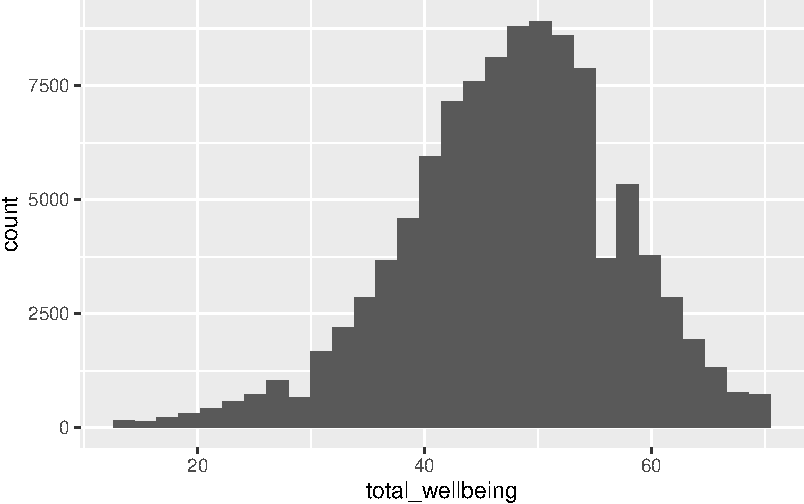
\includegraphics[width=1\textwidth,height=\textheight]{14-multiple-regression_files/figure-pdf/unnamed-chunk-4-1.pdf}
\end{center}

\end{tcolorbox}

\subsection{Activity 4 - Wrangle and visualise the
data}\label{activity-4---wrangle-and-visualise-the-data}

Before we move onto the final modelling stages, we can wrangle the data
to plot the data like the original article. We can plot the relationship
between well-being and hours of technology use, split into four
categories of technology (video games, computers, smartphones, TV).

For this step, we are going to give you the code as there are a few new
functions we have not taught you about. Make sure as you type the code
to question what each line of the code is doing. The functions might be
unfamiliar but you should be able to follow what it is doing. We are
working with many rows here, so the code might take longer to run than
you are used to.

\begin{Shaded}
\begin{Highlighting}[]
\CommentTok{\# Pivot the screen data longer}
\CommentTok{\# Separate the variable into the category and day of the week}
\CommentTok{\# Recode the new variables }
\NormalTok{screen\_long }\OtherTok{\textless{}{-}}\NormalTok{ screen }\SpecialCharTok{\%\textgreater{}\%}
  \FunctionTok{pivot\_longer}\NormalTok{(}\AttributeTok{cols =}\NormalTok{ Comph\_we}\SpecialCharTok{:}\NormalTok{Watch\_wk,}
               \AttributeTok{names\_to =} \StringTok{"var"}\NormalTok{, }
               \AttributeTok{values\_to =} \StringTok{"hours"}\NormalTok{) }\SpecialCharTok{\%\textgreater{}\%}
  \FunctionTok{separate}\NormalTok{(}\AttributeTok{col =}\NormalTok{ var, }\CommentTok{\# split variable name}
           \AttributeTok{into =} \FunctionTok{c}\NormalTok{(}\StringTok{"variable"}\NormalTok{, }\StringTok{"day"}\NormalTok{), }\CommentTok{\# split into two components}
           \AttributeTok{sep =} \StringTok{"\_"}\NormalTok{) }\SpecialCharTok{\%\textgreater{}\%}  \CommentTok{\# split when it sees a \_}
  \FunctionTok{mutate}\NormalTok{(}\AttributeTok{variable =} \FunctionTok{case\_match}\NormalTok{(variable,}
                               \StringTok{"Watch"} \SpecialCharTok{\textasciitilde{}} \StringTok{"Watching TV"}\NormalTok{,}
                               \StringTok{"Comp"} \SpecialCharTok{\textasciitilde{}} \StringTok{"Playing Video Games"}\NormalTok{,}
                               \StringTok{"Comph"} \SpecialCharTok{\textasciitilde{}} \StringTok{"Using Computers"}\NormalTok{,}
                               \StringTok{"Smart"} \SpecialCharTok{\textasciitilde{}} \StringTok{"Using Smartphone"}\NormalTok{),}
         \AttributeTok{day =} \FunctionTok{case\_match}\NormalTok{(day,}
                          \StringTok{"wk"} \SpecialCharTok{\textasciitilde{}} \StringTok{"Weekday"}\NormalTok{,}
                          \StringTok{"we"} \SpecialCharTok{\textasciitilde{}} \StringTok{"Weekend"}\NormalTok{))}

\CommentTok{\# Join the two data sets together }
\CommentTok{\# group by three variables}
\CommentTok{\# calculate the mean well{-}being score}
\NormalTok{dat\_means }\OtherTok{\textless{}{-}}\NormalTok{ wemwbs }\SpecialCharTok{\%\textgreater{}\%} 
  \FunctionTok{inner\_join}\NormalTok{(screen\_long, }
             \AttributeTok{by =} \StringTok{"Serial"}\NormalTok{) }\SpecialCharTok{\%\textgreater{}\%}
  \FunctionTok{group\_by}\NormalTok{(variable, }
\NormalTok{           day, }
\NormalTok{           hours) }\SpecialCharTok{\%\textgreater{}\%}
  \FunctionTok{summarise}\NormalTok{(}\AttributeTok{mean\_wellbeing =} \FunctionTok{mean}\NormalTok{(total\_wellbeing))}
\end{Highlighting}
\end{Shaded}

We now have data at the group level rather than per participant. Each
row of \texttt{dat\_means} is a value for mean well-being split by each
level of variable (technology type), day (weekday or weekend), and hours
of technology use. If you run the following code, we get a line graph
showing the relationship split between technology type and day.

\begin{Shaded}
\begin{Highlighting}[]
\NormalTok{dat\_means }\SpecialCharTok{\%\textgreater{}\%} 
  \FunctionTok{ggplot}\NormalTok{(}\FunctionTok{aes}\NormalTok{(}\AttributeTok{x =}\NormalTok{ hours, }\AttributeTok{y =}\NormalTok{ mean\_wellbeing, }\AttributeTok{linetype =}\NormalTok{ day)) }\SpecialCharTok{+}
  \FunctionTok{geom\_line}\NormalTok{() }\SpecialCharTok{+}
  \FunctionTok{geom\_point}\NormalTok{() }\SpecialCharTok{+}
  \FunctionTok{facet\_wrap}\NormalTok{(}\SpecialCharTok{\textasciitilde{}}\NormalTok{ variable, }\AttributeTok{nrow =} \DecValTok{2}\NormalTok{) }\SpecialCharTok{+} 
  \FunctionTok{theme\_classic}\NormalTok{() }\SpecialCharTok{+} 
  \FunctionTok{labs}\NormalTok{(}\AttributeTok{x =} \StringTok{"Hours of Technology Use"}\NormalTok{,}
       \AttributeTok{y =} \StringTok{"Mean Well{-}Being Score"}\NormalTok{)}
\end{Highlighting}
\end{Shaded}

\begin{center}
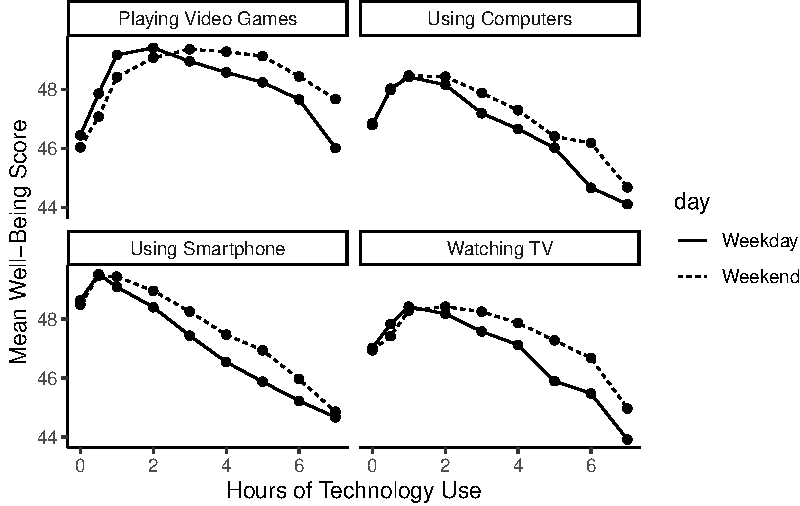
\includegraphics[width=1\textwidth,height=\textheight]{14-multiple-regression_files/figure-pdf/unnamed-chunk-5-1.pdf}
\end{center}

The graph shows that smartphone use of more than 1 hour per day is
associated with increasingly negative well-being. Note that we have
combined the tables using an \texttt{inner\_join()}, such that we only
include data for which we have observations across the \texttt{wemwbs}
and \texttt{screen\_long} tables.

In the next step, we are going to focus on the smartphone/well-being
relationship for our multiple linear regression demonstration.

\section{Multiple linear regression}\label{mulregression-a5}

Now that we have explored the data, we can start preparing for the
analysis. Note that in this analysis, we have:

\begin{itemize}
\item
  A continuous\(^*\) outcome: well-being.
\item
  One continuous\(^*\) predictor: screen time.
\item
  One categorical predictor: gender.
\end{itemize}

\(^*\)these variables are only quasi-continuous as only discrete values
are possible. This returns up to the ordinal dilemma, particularly for
the outcome of well-being. However, there are a sufficient number of
discrete values that we can treat them as effectively continuous.

We want to estimate two slopes relating screen time to well-being, one
for girls and one for boys, and then statistically compare these slopes.
So, this problem seems simultaneously like a situation where you would
run a regression (to estimate the slopes) but also one where you would
need a t-test (to compare two groups). This is the power of regression
models as you can look at the interaction between one continuous and one
categorical predictor, something that is not possible in factorial
ANOVA.

\subsection{Activity 5 - Complete the final wrangling
steps}\label{activity-5---complete-the-final-wrangling-steps}

For this analysis, we are going to average weekday and weekend use for
smartphones. We need one final round of wrangling to prepare for
creating a multiple linear regression model.

\begin{tcolorbox}[enhanced jigsaw, breakable, colframe=quarto-callout-tip-color-frame, arc=.35mm, opacitybacktitle=0.6, titlerule=0mm, colbacktitle=quarto-callout-tip-color!10!white, colback=white, toprule=.15mm, bottomtitle=1mm, toptitle=1mm, title=\textcolor{quarto-callout-tip-color}{\faLightbulb}\hspace{0.5em}{Try this}, bottomrule=.15mm, rightrule=.15mm, leftrule=.75mm, coltitle=black, left=2mm, opacityback=0]

\textbf{Step 1.} Create a new data object \texttt{smarttot} that has the
mean number of hours per day of smartphone use for each participant,
averaged over weekends/weekdays. Then filter the data to only include
those who use a smart phone for more than one hour per day.

To do this, you will need to:

\begin{itemize}
\item
  Filter the data \texttt{screen\_long} to \textbf{only} include
  smartphone use and not other technologies.
\item
  Group the results by the participant ID (\texttt{Serial}).
\item
  Summarise the data to calculate the mean number of hours per
  participant. Call this variable \texttt{total\_hours}.
\item
  Filter the data to only include participants who use a smartphone for
  more than 1 hour per day.
\end{itemize}

The data \texttt{smarttot} should have two variables: \texttt{Serial}
(the participant) and \texttt{total\_hours}.

\textbf{Step 2.} Once you have \texttt{smarttot}, combine (join) this
data object with the information in \texttt{wemwbs} and \texttt{pinfo}.
Call this new object \texttt{smart\_wb}. This is the final object you
need for the multiple linear regression model.

\end{tcolorbox}

\begin{tcolorbox}[enhanced jigsaw, breakable, colframe=quarto-callout-caution-color-frame, arc=.35mm, opacitybacktitle=0.6, titlerule=0mm, colbacktitle=quarto-callout-caution-color!10!white, colback=white, toprule=.15mm, bottomtitle=1mm, toptitle=1mm, title=\textcolor{quarto-callout-caution-color}{\faFire}\hspace{0.5em}{Show me the solution}, bottomrule=.15mm, rightrule=.15mm, leftrule=.75mm, coltitle=black, left=2mm, opacityback=0]

You should have the following in a code chunk:

\begin{Shaded}
\begin{Highlighting}[]
\NormalTok{smarttot }\OtherTok{\textless{}{-}}\NormalTok{ screen\_long }\SpecialCharTok{\%\textgreater{}\%}
  \FunctionTok{filter}\NormalTok{(variable }\SpecialCharTok{==} \StringTok{"Using Smartphone"}\NormalTok{) }\SpecialCharTok{\%\textgreater{}\%}
  \FunctionTok{group\_by}\NormalTok{(Serial) }\SpecialCharTok{\%\textgreater{}\%}
  \FunctionTok{summarise}\NormalTok{(}\AttributeTok{total\_hours =} \FunctionTok{mean}\NormalTok{(hours)) }\SpecialCharTok{\%\textgreater{}\%} 
  \FunctionTok{filter}\NormalTok{(total\_hours }\SpecialCharTok{\textgreater{}} \DecValTok{1}\NormalTok{)}

\NormalTok{smart\_wb }\OtherTok{\textless{}{-}}\NormalTok{ smarttot }\SpecialCharTok{\%\textgreater{}\%}
  \FunctionTok{inner\_join}\NormalTok{(wemwbs, }
             \AttributeTok{by =} \StringTok{"Serial"}\NormalTok{) }\SpecialCharTok{\%\textgreater{}\%}
  \FunctionTok{inner\_join}\NormalTok{(pinfo, }
             \AttributeTok{by =} \StringTok{"Serial"}\NormalTok{) }
\end{Highlighting}
\end{Shaded}

\end{tcolorbox}

\subsection{Activity 6 - Mean-centering
variables}\label{mulregression-a6}

As we discussed in the course materials, when you have continuous
variables in a regression model, it is often sensible to transform them
by \textbf{mean centering}. We covered this in Chapter 8, but it is
particularly important in multiple linear regression. You mean center a
predictor \texttt{X} by subtracting the mean of the predictor
(\texttt{X\_centered\ =\ X\ -\ mean(X)}). This has two useful
consequences:

\begin{itemize}
\item
  The model intercept reflects the prediction for \(Y\) at the mean
  value of the predictor variable, rather than at the zero value of the
  unscaled variable.
\item
  If there are interactions in the model, any lower-order effects can be
  given the same interpretation as they receive in ANOVA (main effects,
  rather than simple effects).
\end{itemize}

For categorical predictors with two levels, these become coded as -.5
and .5 (because the mean of these two values is 0).

\begin{tcolorbox}[enhanced jigsaw, breakable, colframe=quarto-callout-tip-color-frame, arc=.35mm, opacitybacktitle=0.6, titlerule=0mm, colbacktitle=quarto-callout-tip-color!10!white, colback=white, toprule=.15mm, bottomtitle=1mm, toptitle=1mm, title=\textcolor{quarto-callout-tip-color}{\faLightbulb}\hspace{0.5em}{Try this}, bottomrule=.15mm, rightrule=.15mm, leftrule=.75mm, coltitle=black, left=2mm, opacityback=0]

Use \texttt{mutate()} to add two new variables to \texttt{smart\_wb}:

\begin{itemize}
\item
  \texttt{total\_hours\_c}: calculated as a mean-centered version of the
  \texttt{total\_hours} predictor
\item
  \texttt{male\_c}: recoded as -.5 for female and .5 for male, and then
  converts both \texttt{male} and \texttt{male\_c} as factors, so that R
  knows not to treat them as real numbers.
\end{itemize}

\end{tcolorbox}

\begin{tcolorbox}[enhanced jigsaw, breakable, colframe=quarto-callout-caution-color-frame, arc=.35mm, opacitybacktitle=0.6, titlerule=0mm, colbacktitle=quarto-callout-caution-color!10!white, colback=white, toprule=.15mm, bottomtitle=1mm, toptitle=1mm, title=\textcolor{quarto-callout-caution-color}{\faFire}\hspace{0.5em}{Show me the solution}, bottomrule=.15mm, rightrule=.15mm, leftrule=.75mm, coltitle=black, left=2mm, opacityback=0]

You should have the following in a code chunk:

\begin{Shaded}
\begin{Highlighting}[]
\NormalTok{smart\_wb }\OtherTok{\textless{}{-}}\NormalTok{ smart\_wb }\SpecialCharTok{\%\textgreater{}\%}
  \FunctionTok{mutate}\NormalTok{(}\AttributeTok{total\_hours\_c =}\NormalTok{ total\_hours }\SpecialCharTok{{-}} \FunctionTok{mean}\NormalTok{(total\_hours),}
         \AttributeTok{male\_c =} \FunctionTok{case\_when}\NormalTok{(male }\SpecialCharTok{==} \DecValTok{1} \SpecialCharTok{\textasciitilde{}}\NormalTok{ .}\DecValTok{5}\NormalTok{, }
\NormalTok{                            male }\SpecialCharTok{==} \DecValTok{0} \SpecialCharTok{\textasciitilde{}} \SpecialCharTok{{-}}\NormalTok{.}\DecValTok{5}\NormalTok{),}
         \AttributeTok{male\_c =} \FunctionTok{as.factor}\NormalTok{(male\_c),}
         \AttributeTok{male =} \FunctionTok{as.factor}\NormalTok{(male))}
\end{Highlighting}
\end{Shaded}

\end{tcolorbox}

\subsection{Activity 7 - Running the regression}\label{mulregression-a8}

For the data in \texttt{smart\_wb}, use the \texttt{lm()} function to
calculate the multiple regression model:

\(Y_i = \beta_0 + \beta_1 X_{1i}  + \beta_2 X_{2i}  + \beta_3 X_{3i} + e_i\)

where

\begin{itemize}
\item
  \(Y_i\) is the well-being score for participant \(i\);
\item
  \(X_{1i}\) is the mean-centered smartphone use variable for
  participant \(i\);
\item
  \(X_{2i}\) is gender (-.5 = female, .5 = male);
\item
  \(X_{3i}\) is the interaction between smartphone use and gender
  (\(= X_{1i} \times X_{2i}\))
\end{itemize}

\begin{tcolorbox}[enhanced jigsaw, breakable, colframe=quarto-callout-tip-color-frame, arc=.35mm, opacitybacktitle=0.6, titlerule=0mm, colbacktitle=quarto-callout-tip-color!10!white, colback=white, toprule=.15mm, bottomtitle=1mm, toptitle=1mm, title=\textcolor{quarto-callout-tip-color}{\faLightbulb}\hspace{0.5em}{Try this}, bottomrule=.15mm, rightrule=.15mm, leftrule=.75mm, coltitle=black, left=2mm, opacityback=0]

Save your model to the object \texttt{ml\_model}.

Save the \texttt{summary()} of your model to the object
\texttt{model\_summary}.

Print the \texttt{model\_summary} to see the results and answer the
following questions:

\begin{itemize}
\item
  The interaction between smartphone use and gender is shown by the
  variable
\item
  \begin{enumerate}
  \def\labelenumi{(\Alph{enumi})}
  \tightlist
  \item
    thours\_c\\
  \end{enumerate}
\item
  \begin{enumerate}
  \def\labelenumi{(\Alph{enumi})}
  \setcounter{enumi}{1}
  \tightlist
  \item
    male\_c\\
  \end{enumerate}
\item
  \begin{enumerate}
  \def\labelenumi{(\Alph{enumi})}
  \setcounter{enumi}{2}
  \tightlist
  \item
    thours\_c:male\_c
  \end{enumerate}
\end{itemize}

, and this interaction was

\begin{itemize}
\tightlist
\item
  \begin{enumerate}
  \def\labelenumi{(\Alph{enumi})}
  \tightlist
  \item
    significant\\
  \end{enumerate}
\item
  \begin{enumerate}
  \def\labelenumi{(\Alph{enumi})}
  \setcounter{enumi}{1}
  \tightlist
  \item
    non-significant
  \end{enumerate}
\end{itemize}

at the \(\alpha = .05\) level.

\begin{itemize}
\item
  To 2 decimal places, adjusted \(R^2\) suggests the overall model
  explains what percentage of the variance in well-being scores?
  \_\_\_\_
\item
  The \emph{p}-value for the overall model fit is
  \texttt{\textless{}2e-16}. Is this statistically significant?
\item
  \begin{enumerate}
  \def\labelenumi{(\Alph{enumi})}
  \tightlist
  \item
    Yes\\
  \end{enumerate}
\item
  \begin{enumerate}
  \def\labelenumi{(\Alph{enumi})}
  \setcounter{enumi}{1}
  \tightlist
  \item
    No
  \end{enumerate}
\end{itemize}

\end{tcolorbox}

\begin{tcolorbox}[enhanced jigsaw, breakable, colframe=quarto-callout-caution-color-frame, arc=.35mm, opacitybacktitle=0.6, titlerule=0mm, colbacktitle=quarto-callout-caution-color!10!white, colback=white, toprule=.15mm, bottomtitle=1mm, toptitle=1mm, title=\textcolor{quarto-callout-caution-color}{\faFire}\hspace{0.5em}{Show me the solution}, bottomrule=.15mm, rightrule=.15mm, leftrule=.75mm, coltitle=black, left=2mm, opacityback=0]

You should have the following in a code chunk:

\begin{Shaded}
\begin{Highlighting}[]
\NormalTok{ml\_model }\OtherTok{\textless{}{-}} \FunctionTok{lm}\NormalTok{(}\AttributeTok{formula =}\NormalTok{ total\_wellbeing }\SpecialCharTok{\textasciitilde{}}\NormalTok{ total\_hours\_c }\SpecialCharTok{*}\NormalTok{ male\_c, }
               \AttributeTok{data =}\NormalTok{ smart\_wb)}

\NormalTok{mod\_summary }\OtherTok{\textless{}{-}} \FunctionTok{summary}\NormalTok{(ml\_model)}

\NormalTok{mod\_summary}
\end{Highlighting}
\end{Shaded}

\begin{verbatim}

Call:
lm(formula = total_wellbeing ~ total_hours_c * male_c, data = smart_wb)

Residuals:
    Min      1Q  Median      3Q     Max 
-36.881  -5.721   0.408   6.237  27.264 

Coefficients:
                        Estimate Std. Error t value Pr(>|t|)    
(Intercept)             44.86740    0.04478 1001.87   <2e-16 ***
total_hours_c           -0.77121    0.02340  -32.96   <2e-16 ***
male_c0.5                5.13968    0.07113   72.25   <2e-16 ***
total_hours_c:male_c0.5  0.45205    0.03693   12.24   <2e-16 ***
---
Signif. codes:  0 '***' 0.001 '**' 0.01 '*' 0.05 '.' 0.1 ' ' 1

Residual standard error: 9.135 on 71029 degrees of freedom
Multiple R-squared:  0.09381,   Adjusted R-squared:  0.09377 
F-statistic:  2451 on 3 and 71029 DF,  p-value: < 2.2e-16
\end{verbatim}

\end{tcolorbox}

\subsection{Activity 8 - Visualising
interactions}\label{activity-8---visualising-interactions}

It is very difficult to understand an interaction from the coefficient
alone, so your best bet is visualising the interaction to help you
understand the results and communicate your results to your readers.

There is a great package called sjPlot which takes regression models and
helps you plot them in different ways. We will demonstrate plotting
interactions, but for further information and options, see the
\href{https://strengejacke.github.io/sjPlot/articles/plot_interactions.html}{online
documentation}.

To plot the interaction, you need the model object (not the summary),
specify ``pred'' as the \texttt{type} as we want to plot predictions,
and add the \texttt{terms} you want to plot.

\begin{Shaded}
\begin{Highlighting}[]
\FunctionTok{plot\_model}\NormalTok{(ml\_model, }
           \AttributeTok{type =} \StringTok{"pred"}\NormalTok{, }
           \AttributeTok{terms =} \FunctionTok{c}\NormalTok{(}\StringTok{"total\_hours\_c"}\NormalTok{, }\StringTok{"male\_c"}\NormalTok{))}
\end{Highlighting}
\end{Shaded}

\begin{center}
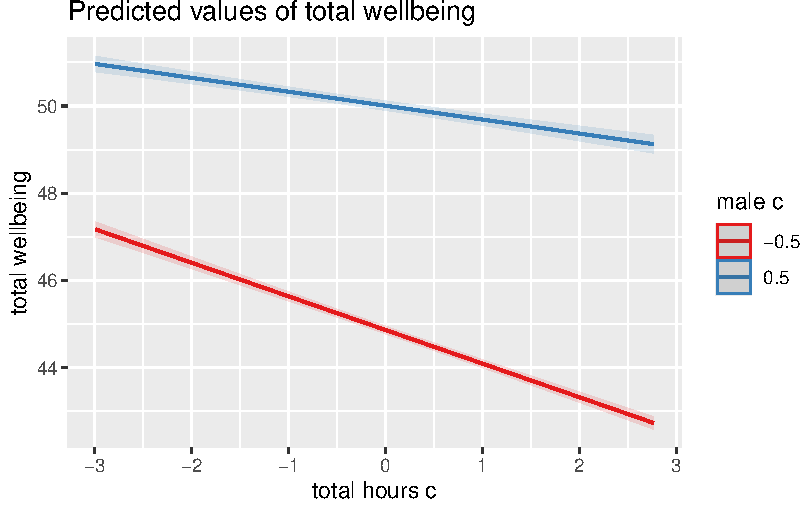
\includegraphics[width=1\textwidth,height=\textheight]{14-multiple-regression_files/figure-pdf/unnamed-chunk-6-1.pdf}
\end{center}

What is the most reasonable interpretation of the interaction?

\begin{itemize}
\tightlist
\item
  \begin{enumerate}
  \def\labelenumi{(\Alph{enumi})}
  \tightlist
  \item
    there is no evidence for gender differences in the relationship
    between smartphone use and well-being\\
  \end{enumerate}
\item
  \begin{enumerate}
  \def\labelenumi{(\Alph{enumi})}
  \setcounter{enumi}{1}
  \tightlist
  \item
    smartphone use harms boys more than girls\\
  \end{enumerate}
\item
  \begin{enumerate}
  \def\labelenumi{(\Alph{enumi})}
  \setcounter{enumi}{2}
  \tightlist
  \item
    smartphone use was more negatively associated with wellbeing for
    girls than for boys\\
  \end{enumerate}
\item
  \begin{enumerate}
  \def\labelenumi{(\Alph{enumi})}
  \setcounter{enumi}{3}
  \tightlist
  \item
    smartphone use harms girls more than boys
  \end{enumerate}
\end{itemize}

This is fine for helping you to interpret your model, but you would need
to customise it before adding it into a report. Like
\texttt{afex\_plot()} we introduced you to in Chapter 13,
\texttt{plot\_model()} uses ggplot2 in the background. You can add
further customisation by adding layers after the initial function.

\begin{tcolorbox}[enhanced jigsaw, breakable, colframe=quarto-callout-note-color-frame, arc=.35mm, opacitybacktitle=0.6, titlerule=0mm, colbacktitle=quarto-callout-note-color!10!white, colback=white, toprule=.15mm, bottomtitle=1mm, toptitle=1mm, title=\textcolor{quarto-callout-note-color}{\faInfo}\hspace{0.5em}{Note}, bottomrule=.15mm, rightrule=.15mm, leftrule=.75mm, coltitle=black, left=2mm, opacityback=0]

Since \texttt{plot\_model()} uses ggplot2, you can use \texttt{ggsave()}
to save your plots and insert them into your work.

\end{tcolorbox}

For example, we can tidy up the axis labels and remove the title, and
set a theme.

\begin{Shaded}
\begin{Highlighting}[]
\FunctionTok{plot\_model}\NormalTok{(ml\_model, }
           \AttributeTok{type =} \StringTok{"pred"}\NormalTok{, }
           \AttributeTok{terms =} \FunctionTok{c}\NormalTok{(}\StringTok{"total\_hours\_c"}\NormalTok{, }\StringTok{"male\_c"}\NormalTok{)) }\SpecialCharTok{+} 
  \FunctionTok{labs}\NormalTok{(}\AttributeTok{x =} \StringTok{"Total Hours Smartphone Use"}\NormalTok{,}
       \AttributeTok{y =} \StringTok{"Total Well{-}Being Score"}\NormalTok{,}
       \AttributeTok{title =} \StringTok{""}\NormalTok{) }\SpecialCharTok{+} 
  \FunctionTok{theme\_classic}\NormalTok{()}
\end{Highlighting}
\end{Shaded}

\begin{center}
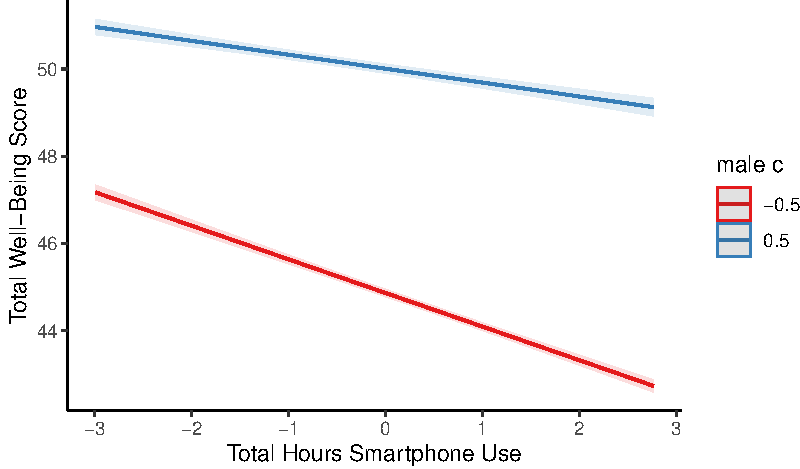
\includegraphics[width=1\textwidth,height=\textheight]{14-multiple-regression_files/figure-pdf/unnamed-chunk-7-1.pdf}
\end{center}

For communicating interactions, it is normally better to plot a version
using the raw predictors instead of the mean centered versions as the
interaction does not change and it will be easier for your readers to
understand.

\subsection{Activity 9 - Assumption checking}\label{mulregression-a9}

Now it's time to test those pesky assumptions. The assumptions for
multiple regression are the same as simple regression but there is one
additional assumption, that of multicollinearity. This is the idea that
predictor variables should not be too highly correlated.

\begin{enumerate}
\def\labelenumi{\arabic{enumi}.}
\item
  The outcome/DV is a interval/ratio level data.
\item
  The predictor variable is interval/ratio or categorical (with two
  levels).
\item
  All values of the outcome variable are independent (i.e., each score
  should come from a different participant).
\item
  The predictors have non-zero variance.
\item
  The relationship between outcome and predictor is linear.
\item
  The residuals should be normally distributed.
\item
  There should be homoscedasticity (homogeneity of variance, but for the
  residuals).
\item
  Multicollinearity: predictor variables should not be too highly
  correlated.
\end{enumerate}

From the work we have done so far, we know that we meet assumptions 1 -
4 and we can use the \texttt{plot()} function for diagnostic plots, plus
\texttt{check\_model()} from the performance package.

One difference from when we used \texttt{check\_model()} previously is
that rather than just letting it run all the tests it wants, we are
going to specify which tests to stop it throwing an error. A word of
warning - these assumption tests will take longer than usual to run
because it's such a big data set. The first line of code will run the
assumption tests and save it to an object, calling the object name will
then display the plots.

\begin{Shaded}
\begin{Highlighting}[]
\NormalTok{assumptions }\OtherTok{\textless{}{-}} \FunctionTok{check\_model}\NormalTok{(ml\_model, }
                           \AttributeTok{check =} \FunctionTok{c}\NormalTok{(}\StringTok{"vif"}\NormalTok{, }
                                     \StringTok{"qq"}\NormalTok{, }
                                     \StringTok{"normality"}\NormalTok{, }
                                     \StringTok{"linearity"}\NormalTok{, }
                                     \StringTok{"homogeneity"}\NormalTok{))}

\NormalTok{assumptions}
\end{Highlighting}
\end{Shaded}

\begin{figure}[H]

\centering{

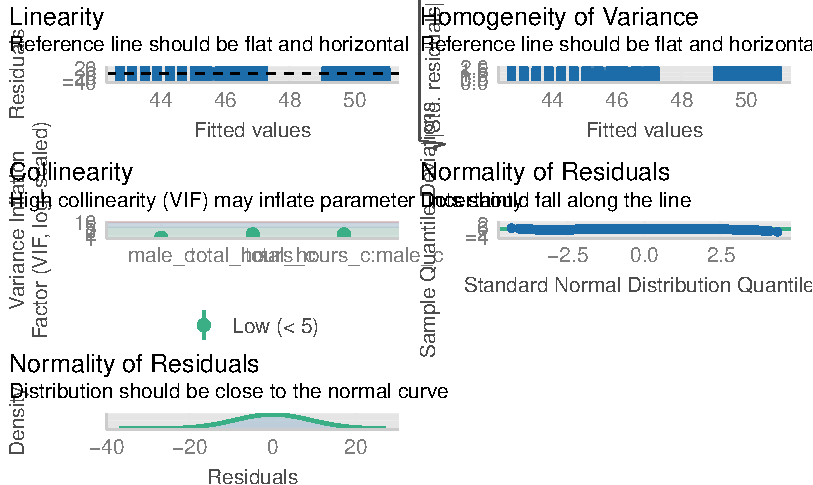
\includegraphics[width=1\textwidth,height=\textheight]{14-multiple-regression_files/figure-pdf/fig-assumption-plots-1.pdf}

}

\caption{\label{fig-assumption-plots}Assumption plots from the
performance package.}

\end{figure}%

For assumption 5, linearity, we already know from looking at the
scatterplot that the relationship is linear, but the residual plot also
confirms this.

For assumption 6, normality of residuals, the residuals look good in
both plots and this provides an excellent example of why it's often
better to visualise than rely on statistics. With a sample size this
large, any statistical diagnostic tests will be highly significant as
they are sensitive to sample size.

For assumption 7, homoscedasticity, the plot is missing the reference
line. Fun fact, this took us several days of our lives and asking for
help on social media to figure out. The reason the line is not there is
because the data set is so large that is creates a memory issue.
However, if you use the \texttt{plot()} version, it does show the
reference line.

\begin{Shaded}
\begin{Highlighting}[]
\FunctionTok{plot}\NormalTok{(ml\_model,}
     \AttributeTok{which =} \DecValTok{3}\NormalTok{)}
\end{Highlighting}
\end{Shaded}

\begin{center}
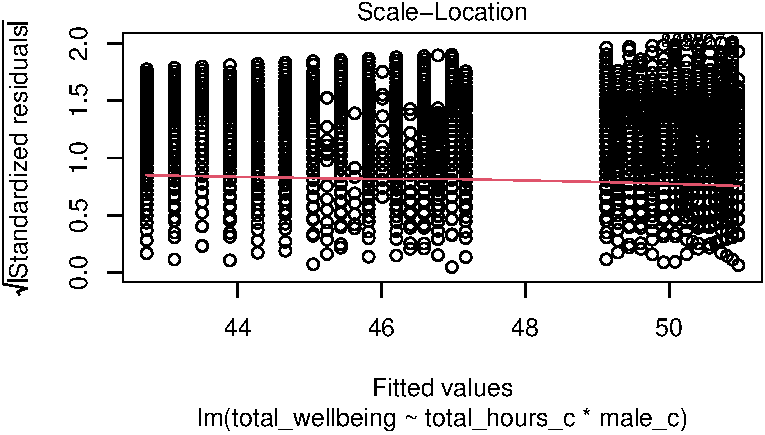
\includegraphics[width=1\textwidth,height=\textheight]{14-multiple-regression_files/figure-pdf/unnamed-chunk-8-1.pdf}
\end{center}

It is not perfect, but the reference line is roughly flat to suggest
there are no serious issues with homoscedasticity.

Finally, for assumption 8, multicollinearity, the plot also indicates no
issues but we can also test this statistically using
\texttt{check\_collinearity()} to produce VIF (variance inflation
factor) and tolerance values.

Essentially, this function estimates how much the variance of a
coefficient is ``inflated'' because of linear dependence with other
predictors, i.e., that a predictor is not actually adding any unique
variance to the model, it's just really strongly related to other
predictors. \href{https://statisticalhorizons.com/multicollinearity}{You
can read more about this online}. Thankfully, VIF is not affected by
large samples like other statistical diagnostic tests.

There are various rules of thumb, but most converge on a VIF of above 2
- 2.5 for any one predictor being problematic.

\begin{Shaded}
\begin{Highlighting}[]
\FunctionTok{check\_collinearity}\NormalTok{(ml\_model)}
\end{Highlighting}
\end{Shaded}

\begin{verbatim}
# Check for Multicollinearity

Low Correlation

                 Term  VIF   VIF 95% CI Increased SE Tolerance Tolerance 95% CI
        total_hours_c 1.72 [1.70, 1.74]         1.31      0.58     [0.57, 0.59]
               male_c 1.04 [1.03, 1.04]         1.02      0.97     [0.96, 0.97]
 total_hours_c:male_c 1.72 [1.70, 1.73]         1.31      0.58     [0.58, 0.59]
\end{verbatim}

\subsection{Activity 10 - Power and effect
sizes}\label{mulregression-a10}

Finally, we will calculate power and an effect size specific to multiple
linear regression. Your coefficients represent the effect size for
individual variables, but you can summarise the whole regression model
with \(R^2\) and \(f^2\).

Using your understanding of power analysis from Chapter 10 and the
function specific to regression models, calculate the minimum effect
size we could reliably observe given our sample size and design but for
99\% power and 5\% alpha.

Hint: for \texttt{v}, it is the sample size minus u minus 1 (\texttt{N}
- \texttt{u} - \texttt{1})

\begin{Shaded}
\begin{Highlighting}[]
\FunctionTok{pwr.f2.test}\NormalTok{(}\AttributeTok{u =}\NormalTok{ ?, }
            \AttributeTok{v =}\NormalTok{ ?, }
            \AttributeTok{f2 =} \ConstantTok{NULL}\NormalTok{, }
            \AttributeTok{sig.level =}\NormalTok{ ?, }
            \AttributeTok{power =}\NormalTok{ ?)}
\end{Highlighting}
\end{Shaded}

To 2 decimals, what is the value of \(f^2\) the study would be sensitive
to?

\begin{tcolorbox}[enhanced jigsaw, breakable, colframe=quarto-callout-caution-color-frame, arc=.35mm, opacitybacktitle=0.6, titlerule=0mm, colbacktitle=quarto-callout-caution-color!10!white, colback=white, toprule=.15mm, bottomtitle=1mm, toptitle=1mm, title=\textcolor{quarto-callout-caution-color}{\faFire}\hspace{0.5em}{Show me the solution}, bottomrule=.15mm, rightrule=.15mm, leftrule=.75mm, coltitle=black, left=2mm, opacityback=0]

You should have the following in a code chunk:

\begin{Shaded}
\begin{Highlighting}[]
\FunctionTok{pwr.f2.test}\NormalTok{(}\AttributeTok{u =} \DecValTok{3}\NormalTok{, }
            \AttributeTok{v =} \DecValTok{71029}\NormalTok{, }
            \AttributeTok{f2 =} \ConstantTok{NULL}\NormalTok{, }
            \AttributeTok{sig.level =}\NormalTok{ .}\DecValTok{05}\NormalTok{, }
            \AttributeTok{power =}\NormalTok{ .}\DecValTok{99}\NormalTok{)}
\end{Highlighting}
\end{Shaded}

\begin{verbatim}

     Multiple regression power calculation 

              u = 3
              v = 71029
             f2 = 0.0003673651
      sig.level = 0.05
          power = 0.99
\end{verbatim}

The study was incredibly sensitive, where they would detect effects of
\(f^2\) = .0004 with 99\% power.

\end{tcolorbox}

The effect size \(f^2\) is a kind of transformed version of \(R^2\). You
can calculate it through the equation:

\(f^2 = \frac{adj R^2}{1 - adj R^2}\)

Or as code:

\begin{Shaded}
\begin{Highlighting}[]
\NormalTok{f2 }\OtherTok{\textless{}{-}}\NormalTok{ adj\_R2}\SpecialCharTok{/}\NormalTok{(}\DecValTok{1} \SpecialCharTok{{-}}\NormalTok{ adj\_R2)}
\end{Highlighting}
\end{Shaded}

\begin{tcolorbox}[enhanced jigsaw, breakable, colframe=quarto-callout-tip-color-frame, arc=.35mm, opacitybacktitle=0.6, titlerule=0mm, colbacktitle=quarto-callout-tip-color!10!white, colback=white, toprule=.15mm, bottomtitle=1mm, toptitle=1mm, title=\textcolor{quarto-callout-tip-color}{\faLightbulb}\hspace{0.5em}{Try this}, bottomrule=.15mm, rightrule=.15mm, leftrule=.75mm, coltitle=black, left=2mm, opacityback=0]

Calculate the \(f^2\) value from the multiple regression model using one
of these methods. Try and use the values directly from the model object
to avoid typing in the values.

What is the observed effect size (in \(f^2\)) for the study to 2 decimal
places? \_\_\_

\end{tcolorbox}

\begin{tcolorbox}[enhanced jigsaw, breakable, colframe=quarto-callout-caution-color-frame, arc=.35mm, opacitybacktitle=0.6, titlerule=0mm, colbacktitle=quarto-callout-caution-color!10!white, colback=white, toprule=.15mm, bottomtitle=1mm, toptitle=1mm, title=\textcolor{quarto-callout-caution-color}{\faFire}\hspace{0.5em}{Show me the solution}, bottomrule=.15mm, rightrule=.15mm, leftrule=.75mm, coltitle=black, left=2mm, opacityback=0]

You should have the following in a code chunk:

\begin{Shaded}
\begin{Highlighting}[]
\NormalTok{f2 }\OtherTok{\textless{}{-}}\NormalTok{ mod\_summary}\SpecialCharTok{$}\NormalTok{adj.r.squared}\SpecialCharTok{/}\NormalTok{(}\DecValTok{1} \SpecialCharTok{{-}}\NormalTok{ mod\_summary}\SpecialCharTok{$}\NormalTok{adj.r.squared)}

\NormalTok{f2}
\end{Highlighting}
\end{Shaded}

\begin{verbatim}
[1] 0.1034697
\end{verbatim}

\end{tcolorbox}

Comparing the observed effect size against the effect size the study was
sensitive to with 99\% power, do you think the study was sufficiently
powered?

\begin{itemize}
\tightlist
\item
  \begin{enumerate}
  \def\labelenumi{(\Alph{enumi})}
  \tightlist
  \item
    Yes\\
  \end{enumerate}
\item
  \begin{enumerate}
  \def\labelenumi{(\Alph{enumi})}
  \setcounter{enumi}{1}
  \tightlist
  \item
    No
  \end{enumerate}
\end{itemize}

\section{Reporting the results of multiple linear
regression}\label{mulregression-a11}

The same as previous chapters like ANOVA and factorial ANOVA, we can use
inline code to help with the write-up. First, copy and paste the code
below into \textbf{white-space} in your R Markdown document and then
knit. Note that we enter the \emph{p}-values manually because of the APA
``\emph{p} \textless{} .001'' formatting.

\begin{Shaded}
\begin{Highlighting}[]
\NormalTok{All continuous predictors were mean}\SpecialCharTok{{-}}\NormalTok{centered and deviation coding was used }\ControlFlowTok{for}\NormalTok{ categorical predictors. The results of the regression indicated that the model significantly predicted course }\FunctionTok{engagement}\NormalTok{ (}\FunctionTok{F}\NormalTok{(}\StringTok{\textasciigrave{}}\AttributeTok{r mod\_summary$fstatistic[2]}\StringTok{\textasciigrave{}}\NormalTok{, }\StringTok{\textasciigrave{}}\AttributeTok{r mod\_summary$fstatistic[3] \%\textgreater{}\% round(2)}\StringTok{\textasciigrave{}}\NormalTok{) }\OtherTok{=} \StringTok{\textasciigrave{}}\AttributeTok{r mod\_summary$fstatistic[1] \%\textgreater{}\% round(2)}\StringTok{\textasciigrave{}}\NormalTok{, p }\SpecialCharTok{\textless{}}\NormalTok{ .}\DecValTok{001}\NormalTok{, Adjusted }\AttributeTok{R2 =} \StringTok{\textasciigrave{}}\AttributeTok{r mod\_summary$adj.r.squared \%\textgreater{}\% round(2)}\StringTok{\textasciigrave{}}\NormalTok{, f}\SpecialCharTok{\^{}}\DecValTok{2}\SpecialCharTok{\^{}} \ErrorTok{=} \StringTok{\textasciigrave{}}\AttributeTok{r f2\%\textgreater{}\% round(2)}\StringTok{\textasciigrave{}}\NormalTok{), accounting }\ControlFlowTok{for} \StringTok{\textasciigrave{}}\AttributeTok{r (mod\_summary$adj.r.squared \%\textgreater{}\% round(2))*100}\StringTok{\textasciigrave{}}\SpecialCharTok{\% of the variance. Total screen time was a significant negative predictor of wellbeing scores (β = \textasciigrave{}r ml\_model$coefficients[2] \%}\ErrorTok{\textgreater{}}\SpecialCharTok{\% round(2)\textasciigrave{}, *p* \textless{} .001, as was gender (β = \textasciigrave{}r ml\_model$coefficients[3] \%}\ErrorTok{\textgreater{}}\SpecialCharTok{\% round(2)\textasciigrave{}, *p* \textless{} .001, with girls having lower wellbeing scores than boys. Importantly, there was a significant interaction between screentime and gender (β = \textasciigrave{}r ml\_model$coefficients[4] \%}\ErrorTok{\textgreater{}}\NormalTok{\% }\FunctionTok{round}\NormalTok{(}\DecValTok{2}\NormalTok{)}\StringTok{\textasciigrave{}}\AttributeTok{, *p* \textless{} .001), smartphone use was more negatively associated with wellbeing for girls than for boys. }
\end{Highlighting}
\end{Shaded}

\begin{quote}
All continuous predictors were mean-centered and deviation coding was
used for categorical predictors. The results of the regression indicated
that the model significantly predicted course engagement (F(3,
\ensuremath{7.1029\times 10^{4}}) = 2450.89, p \textless{} .001,
Adjusted R2 = 0.09, f\textsuperscript{2} = 0.1), accounting for 9\% of
the variance. Total screen time was a significant negative predictor of
wellbeing scores (β = -0.77, \emph{p} \textless{} .001, as was gender (β
= 5.14, \emph{p} \textless{} .001, with girls having lower wellbeing
scores than boys. Importantly, there was a significant interaction
between screentime and gender (β = 0.45, \emph{p} \textless{} .001),
smartphone use was more negatively associated with wellbeing for girls
than for boys.
\end{quote}

\section{End of Chapter}\label{mulregression-fin}

You are done!

Not just with this chapter but with the R/RStudio component of Research
Methods 2. The progress that you have made is truly astonishing. Even if
you struggled with R/RStudio and have not quite understood every single
line of code, what you are capable of with data wrangling and
visualisation alone makes you some of the most highly competitive
psychology graduates in the world. Try and think of everything you have
learnt from week 1 of Research Methods 1 to now. Hopefully, you have
proved to yourself you can do this.

Regardless of whether you continue with quantitative methods and using
R/RStudio, remember the more important critical skills that you have
learned as part of this process. The next time you see a data set or you
see data being talked about in the news, think about all the work that
was put into getting the data into the final format. More importantly,
think about all the decisions that the researcher needed to make along
the way and how that might have affected the outcome.

\bookmarksetup{startatroot}

\chapter*{Data Analysis Journeys}\label{data-analysis-journeys}
\addcontentsline{toc}{chapter}{Data Analysis Journeys}

\markboth{Data Analysis Journeys}{Data Analysis Journeys}

\bookmarksetup{startatroot}

\chapter{Analysis Journey 1: Data Wrangling}\label{journey-01-wrangling}

Welcome to the first data analysis journey. We have designed these
chapters as a bridge between the structured learning in the core
chapters and your assessments. We present you with a new data set, show
you what the end product should look like, and see if you can apply your
data wrangling, visualisation, and/or analysis skills to get there.

As you gain independence, this is the crucial skill. Data analysis is
all about seeing the data you have available to you and identifying what
the end product needs to be to apply your visualisation and analysis
techniques. You can then mentally (or physically) create a checklist of
tasks to work backwards to get there. There might be a lot of trial and
error as you try one thing, it does not quite work, so you go back and
try something else. If you get stuck though, we have a range of hints
and task lists you can unhide, then the solution to check your attempts
against.

In this first data analysis journey, we focus on data wrangling to apply
all the skills you developed from Chapter 1 to Chapter 6.

\section{Task preparation}\label{task-preparation}

\subsection{Introduction to the data
set}\label{introduction-to-the-data-set-10}

For this task, we are using open data from J. E. Bartlett et al. (2022).
The abstract of their article is:

\begin{quote}
Both daily and non-daily smokers find it difficult to quit smoking
long-term. One factor associated with addictive behaviour is attentional
bias, but previous research in daily and non-daily smokers found
inconsistent results and did not report the reliability of their
cognitive tasks. Using an online sample, we compared daily (n = 106) and
non-daily (n = 60) smokers in their attentional bias towards smoking
pictures. Participants completed a visual probe task with two picture
presentation times: 200ms and 500ms. In confirmatory analyses, there
were no significant effects of interest, and in exploratory analyses,
equivalence testing showed the effects were statistically equivalent to
zero. The reliability of the visual probe task was poor, meaning it
should not be used for repeated testing or investigating individual
differences. The results can be interpreted in line with contemporary
theories of attentional bias where there are unlikely to be stable
trait-like differences between smoking groups. Future research in
attentional bias should focus on state-level differences using more
reliable measures than the visual probe task.
\end{quote}

To summarise, they compared two daily and non-daily smokers on something
called attentional bias. This is the idea that when people use drugs
often, things associated with those drugs grab people's attention.

To measure attentional bias, participants completed a dot probe task.
This is a computer task where participants see two pictures
side-by-side: one related to smoking like someone holding a cigarette
and one unrelated to smoking like someone holding a fork. Both the
images disappear and a small dot appears in the location of one of the
images. Participants must press left or right on the keyboard to
identify where the dot appeared. This process is repeated many times for
different images, different locations of the dot, and different
durations of showing the images. The idea is if smoking images grab
people's attention, they will be able to identify the dot location
faster on average when it appears in the location of the smoking images
compared to when it appears in the location of the the non-smoking
images.

Response time tasks like this are incredibly common in psychology and
cognitive neuroscience, and being able to wrangle hundreds of trials is
a great demonstration of your new data skills. After setting up your
files and project for the chapter, we will outline the kind of problems
you are trying to solve.

\subsection{Organising your files and project for the
task}\label{organising-your-files-and-project-for-the-task}

Before we can get started, you need to organise your files and project
for the task, so your working directory is in order.

\begin{enumerate}
\def\labelenumi{\arabic{enumi}.}
\item
  In your folder for research methods and the book
  \texttt{ResearchMethods1\_2/Quant\_Fundamentals}, create a new folder
  for the data analysis journey called \texttt{Journey\_01\_wrangling}.
  Within \texttt{Journey\_01\_wrangling}, create two new folders called
  \texttt{data} and \texttt{figures}.
\item
  Create an R Project for \texttt{Journey\_01\_wrangling} as an existing
  directory for your chapter folder. This should now be your working
  directory.
\item
  Create a new R Markdown document and give it a sensible title
  describing the chapter, such as
  \texttt{Analysis\ Journey\ 1\ -\ Data\ Wrangling}. Delete everything
  below line 10 so you have a blank file to work with and save the file
  in your \texttt{Journey\_01\_wrangling} folder.
\item
  We are working with data separated into two files. The links are data
  file one
  (\href{data/Bartlett_demographics.csv}{Bartlett\_demographics.csv})
  and data file two
  (\href{data/Bartlett_trials.csv}{Bartlett\_trials.csv}). Right click
  the links and select ``save link as'', or clicking the links will save
  the files to your Downloads. Make sure that both files are saved as
  ``.csv''. Save or copy the file to your \texttt{data/} folder within
  \texttt{Journey\_01\_wrangling}.
\end{enumerate}

You are now ready to start working on the task!

\section{Overview}\label{overview-1}

\subsection{Load tidyverse and read the data
files}\label{load-tidyverse-and-read-the-data-files}

Before we explore what wrangling we need to do, load tidyverse and read
the two data files. As a prompt, save the data files to these object
names to be consistent with the activities below, but you can check the
solution if you are stuck.

\begin{Shaded}
\begin{Highlighting}[]
\CommentTok{\# Load the tidyverse package below}
\FunctionTok{library}\NormalTok{(tidyverse)}

\CommentTok{\# Load the data files}
\CommentTok{\# This should be the Bartlett\_demographics.csv file }
\NormalTok{demog }\OtherTok{\textless{}{-}}\NormalTok{ ?}

\CommentTok{\# This should be the Bartlett\_trials.csv file }
\NormalTok{trials }\OtherTok{\textless{}{-}}\NormalTok{ ?}
\end{Highlighting}
\end{Shaded}

\begin{tcolorbox}[enhanced jigsaw, breakable, colframe=quarto-callout-tip-color-frame, arc=.35mm, opacitybacktitle=0.6, titlerule=0mm, colbacktitle=quarto-callout-tip-color!10!white, colback=white, toprule=.15mm, bottomtitle=1mm, toptitle=1mm, title=\textcolor{quarto-callout-tip-color}{\faLightbulb}\hspace{0.5em}{Show me the solution}, bottomrule=.15mm, rightrule=.15mm, leftrule=.75mm, coltitle=black, left=2mm, opacityback=0]

You should have the following in a code chunk:

\begin{Shaded}
\begin{Highlighting}[]
\CommentTok{\# Load the tidyverse package below}
\FunctionTok{library}\NormalTok{(tidyverse)}

\CommentTok{\# Load the data files}
\CommentTok{\# This should be the Bartlett\_demographics.csv file }
\NormalTok{demog }\OtherTok{\textless{}{-}} \FunctionTok{read\_csv}\NormalTok{(}\StringTok{"data/Bartlett\_demographics.csv"}\NormalTok{)}

\CommentTok{\# This should be the Bartlett\_trials.csv file }
\NormalTok{trials }\OtherTok{\textless{}{-}} \FunctionTok{read\_csv}\NormalTok{(}\StringTok{"data/Bartlett\_trials.csv"}\NormalTok{)}
\end{Highlighting}
\end{Shaded}

\end{tcolorbox}

\subsection{\texorpdfstring{Explore \texttt{demog} and
\texttt{trials}}{Explore demog and trials}}\label{explore-demog-and-trials}

The data from J. E. Bartlett et al. (2022) is split into two data files.
In \texttt{demog}, we have the participant ID
(\texttt{participant\_private\_id}) and several demographic variables.

\begin{verbatim}
Rows: 205
Columns: 20
$ participant_private_id <dbl> 631737, 631738, 631741, 631739, 631749, 631746,~
$ consent_given          <dbl> 1, 1, 1, 1, 1, 1, 1, 1, 1, 1, 1, 1, 1, 1, 1, 1,~
$ age                    <dbl> 46, 54, 23, 34, 38, 19, 25, 21, 28, 35, 47, 45,~
$ cigarettes_per_week    <chr> "Yes", "Yes", "Yes", "Yes", "Yes", "Yes", "Yes"~
$ smoke_everyday         <chr> "Yes", "Yes", "Yes", "Yes", "Yes", "Yes", "Yes"~
$ past_four_weeks        <chr> "Yes", "Yes", "Yes", "Yes", "Yes", "Yes", "Yes"~
$ age_started_smoking    <chr> "12", "17", "17", "16", "15", "16", "22", "11",~
$ country_of_origin      <chr> "United Kingdom", "Germany", "Poland", "Austral~
$ cpd                    <chr> "6", "5", "10", "20", "10", "1", "6", "15", "12~
$ ethnicity              <chr> "White / Caucasian", "White / Caucasian", "Mixe~
$ gender                 <chr> "Female", "Female", "Male", "Female", "Female",~
$ last_cigarette         <chr> "60", "780", "90", "5", "60", "720", "10", "10"~
$ level_education        <chr> "Graduated University / College", "Graduated Un~
$ technical_issues       <chr> "No", "No", "No", "No", "No", "No", "No", "No",~
$ FTND_1                 <dbl> 2, 0, 0, 3, 3, 0, 1, 2, 1, 3, 2, 2, 2, 1, 2, 0,~
$ FTND_2                 <dbl> 0, 0, 0, 0, 0, 0, 0, 1, 0, 0, 1, 1, 0, 1, 0, 0,~
$ FTND_3                 <dbl> 1, 0, 1, 1, 1, 1, 1, 0, 1, 1, 1, 0, 1, 0, 1, 0,~
$ FTND_4                 <dbl> 0, 0, 1, 1, 0, 1, 1, 0, 0, 0, 1, 1, 1, 0, 1, 1,~
$ FTND_5                 <dbl> 0, 0, 0, 1, 1, 1, 0, 1, 1, 1, 1, 0, 1, 1, 0, 0,~
$ FTND_6                 <dbl> 0, 0, 0, 1, 0, 0, 0, 1, 1, 1, 1, 1, 1, 0, 0, 0,~
\end{verbatim}

The columns (variables) we have in the data set are:

\begin{longtable}[]{@{}
  >{\centering\arraybackslash}p{(\columnwidth - 4\tabcolsep) * \real{0.1951}}
  >{\raggedright\arraybackslash}p{(\columnwidth - 4\tabcolsep) * \real{0.4146}}
  >{\raggedright\arraybackslash}p{(\columnwidth - 4\tabcolsep) * \real{0.3902}}@{}}
\toprule\noalign{}
\begin{minipage}[b]{\linewidth}\centering
Variable
\end{minipage} & \begin{minipage}[b]{\linewidth}\raggedright
Type
\end{minipage} & \begin{minipage}[b]{\linewidth}\raggedright
Description
\end{minipage} \\
\midrule\noalign{}
\endhead
\bottomrule\noalign{}
\endlastfoot
participant\_private\_id & double & Participant number. \\
consent\_given & double & 1 = informed consent, 2 = no consent. \\
age & double & Age in Years. \\
cigarettes\_per\_week & character & Do you smoke every week? Yes or
No. \\
smoke\_everyday & character & Do you smoke everyday? Yes or No. \\
past\_four\_weeks & character & Have you smoked in the past four weeks?
Yes or No. \\
age\_started\_smoking & character & Age started smoking in years. \\
country\_of\_origin & character & Country of origin. \\
cpd & character & How many cigarettes do you smoke per day? \\
ethnicity & character & What is your ethniciity? \\
gender & character & What is your gender? \\
last\_cigarette & character & How long in minutes since your last
cigarette? \\
level\_education & character & What is your highest level of
education? \\
technical\_issues & character & Did you experience any technical issues?
Yes or No \\
FTND\_1 to FTND\_6 & double & Six items of the Fagerstrom Test for
Nicotine Dependence \\
\end{longtable}

In \texttt{trials}, we then have the participant ID
(\texttt{participant\_private\_id}) and trial-by-trial information from
the software Gorilla (an online experiment service). This is probably
the biggest data set you have come across so far as we have hundreds of
trials per participant.

\begin{verbatim}
Rows: 244,847
Columns: 15
$ participant_private_id <dbl> 631737, 631737, 631737, 631737, 631737, 631737,~
$ trial_number           <chr> "BEGIN TASK", "1", "1", "1", "1", "2", "2", "2"~
$ reaction_time          <dbl> NA, 8007.015, 249.823, 199.765, 1999.671, 249.8~
$ response               <chr> NA, NA, NA, NA, NA, NA, NA, NA, NA, NA, NA, NA,~
$ correct                <dbl> 0, 0, 0, 0, 0, 0, 0, 0, 0, 0, 0, 0, 0, 0, 0, 0,~
$ display                <chr> NA, "instructions", "practice", "practice", "pr~
$ answer                 <chr> NA, NA, "right", "right", "right", "left", "lef~
$ soa                    <dbl> NA, NA, 200, 200, 200, 200, 200, 200, 500, 500,~
$ screen_name            <chr> NA, "instructions_continue", "Screen 1", "Scree~
$ image_left             <chr> NA, NA, "p1.jpg", "p1.jpg", "p1.jpg", "p1.jpg",~
$ image_right            <chr> NA, NA, "p2.jpg", "p2.jpg", "p2.jpg", "p2.jpg",~
$ dot_left               <chr> NA, NA, "nodot.jpg", "nodot.jpg", "nodot.jpg", ~
$ dot_right              <chr> NA, NA, "dot.jpg", "dot.jpg", "dot.jpg", "nodot~
$ trial_type             <chr> NA, NA, "practice", "practice", "practice", "pr~
$ block                  <dbl> NA, NA, 0, 0, 0, 0, 0, 0, 0, 0, 0, 0, 0, 0, 0, ~
\end{verbatim}

The columns (variables) we have in the data set are:

\begin{longtable}[]{@{}
  >{\centering\arraybackslash}p{(\columnwidth - 4\tabcolsep) * \real{0.1951}}
  >{\raggedright\arraybackslash}p{(\columnwidth - 4\tabcolsep) * \real{0.4146}}
  >{\raggedright\arraybackslash}p{(\columnwidth - 4\tabcolsep) * \real{0.3902}}@{}}
\toprule\noalign{}
\begin{minipage}[b]{\linewidth}\centering
Variable
\end{minipage} & \begin{minipage}[b]{\linewidth}\raggedright
Type
\end{minipage} & \begin{minipage}[b]{\linewidth}\raggedright
Description
\end{minipage} \\
\midrule\noalign{}
\endhead
\bottomrule\noalign{}
\endlastfoot
participant\_private\_id & double & Participant number. \\
trial\_number & character & Trial number as an integer, plus start and
end task. \\
reaction\_time & double & Participant response time in milliseconds
(ms) \\
response & character & Keyboard response from participant. Left or
Right. \\
correct & double & Was the response correct? 1 = correct, 0 =
incorrect. \\
display & character & Trial display: e.g., practice, trials,
instructions, breaks. \\
answer & character & What is the correct answer? Left or Right. \\
soa & double & Stimulus onset asynchrony. How long the images were shown
for: 200ms or 500ms. \\
screen\_name & character & Name of the screen: e.g., screen 1, fixation,
stimuli, response. \\
image\_left & character & Name of the image file in the left area. \\
image\_right & character & Name of the image file in the right area. \\
dot\_left & character & Name of the dot image file in the left area. \\
dot\_right & character & Name of the dot image file in the right
area. \\
trial\_type & character & Category of the trial: practice, neutral,
nonsmoking, smoking. \\
block & double & Number of the trial block. \\
\end{longtable}

\begin{tcolorbox}[enhanced jigsaw, breakable, colframe=quarto-callout-tip-color-frame, arc=.35mm, opacitybacktitle=0.6, titlerule=0mm, colbacktitle=quarto-callout-tip-color!10!white, colback=white, toprule=.15mm, bottomtitle=1mm, toptitle=1mm, title=\textcolor{quarto-callout-tip-color}{\faLightbulb}\hspace{0.5em}{Try this}, bottomrule=.15mm, rightrule=.15mm, leftrule=.75mm, coltitle=black, left=2mm, opacityback=0]

Now we have introduced the two data sets, explore them using different
methods we introduced. For example, opening the data objects as a tab to
scroll around, explore with \texttt{glimpse()}, or even try plotting
some of the variables to see what they look like using visualisation
skills from Chapter 3.

Do you notice any variables that look the wrong type? Can you see any
responses in there that are going to cause problems?

\end{tcolorbox}

\section{Wrangling demographics}\label{wrangling-demographics}

For this kind of data, we recommend wrangling each file first, before
joining them together. Starting with the demographics file, there are a
few wrangling steps before the data are ready to summarise. We are going
to show you a preview of the starting data set and the end product we
are aiming for.

\subsubsection{Raw data}

\begin{verbatim}
Rows: 205
Columns: 20
$ participant_private_id <dbl> 631737, 631738, 631741, 631739, 631749, 631746,~
$ consent_given          <dbl> 1, 1, 1, 1, 1, 1, 1, 1, 1, 1, 1, 1, 1, 1, 1, 1,~
$ age                    <dbl> 46, 54, 23, 34, 38, 19, 25, 21, 28, 35, 47, 45,~
$ cigarettes_per_week    <chr> "Yes", "Yes", "Yes", "Yes", "Yes", "Yes", "Yes"~
$ smoke_everyday         <chr> "Yes", "Yes", "Yes", "Yes", "Yes", "Yes", "Yes"~
$ past_four_weeks        <chr> "Yes", "Yes", "Yes", "Yes", "Yes", "Yes", "Yes"~
$ age_started_smoking    <chr> "12", "17", "17", "16", "15", "16", "22", "11",~
$ country_of_origin      <chr> "United Kingdom", "Germany", "Poland", "Austral~
$ cpd                    <chr> "6", "5", "10", "20", "10", "1", "6", "15", "12~
$ ethnicity              <chr> "White / Caucasian", "White / Caucasian", "Mixe~
$ gender                 <chr> "Female", "Female", "Male", "Female", "Female",~
$ last_cigarette         <chr> "60", "780", "90", "5", "60", "720", "10", "10"~
$ level_education        <chr> "Graduated University / College", "Graduated Un~
$ technical_issues       <chr> "No", "No", "No", "No", "No", "No", "No", "No",~
$ FTND_1                 <dbl> 2, 0, 0, 3, 3, 0, 1, 2, 1, 3, 2, 2, 2, 1, 2, 0,~
$ FTND_2                 <dbl> 0, 0, 0, 0, 0, 0, 0, 1, 0, 0, 1, 1, 0, 1, 0, 0,~
$ FTND_3                 <dbl> 1, 0, 1, 1, 1, 1, 1, 0, 1, 1, 1, 0, 1, 0, 1, 0,~
$ FTND_4                 <dbl> 0, 0, 1, 1, 0, 1, 1, 0, 0, 0, 1, 1, 1, 0, 1, 1,~
$ FTND_5                 <dbl> 0, 0, 0, 1, 1, 1, 0, 1, 1, 1, 1, 0, 1, 1, 0, 0,~
$ FTND_6                 <dbl> 0, 0, 0, 1, 0, 0, 0, 1, 1, 1, 1, 1, 1, 0, 0, 0,~
\end{verbatim}

\subsubsection{Wrangled data}

\begin{verbatim}
Rows: 205
Columns: 22
$ participant_private_id <dbl> 631737, 631738, 631741, 631739, 631749, 631746,~
$ consent_given          <dbl> 1, 1, 1, 1, 1, 1, 1, 1, 1, 1, 1, 1, 1, 1, 1, 1,~
$ age                    <dbl> 46, 54, 23, 34, 38, 19, 25, 21, 28, 35, 47, 45,~
$ cigarettes_per_week    <chr> "Yes", "Yes", "Yes", "Yes", "Yes", "Yes", "Yes"~
$ smoke_everyday         <chr> "Yes", "Yes", "Yes", "Yes", "Yes", "Yes", "Yes"~
$ past_four_weeks        <chr> "Yes", "Yes", "Yes", "Yes", "Yes", "Yes", "Yes"~
$ age_started_smoking    <int> 12, 17, 17, 16, 15, 16, 22, 11, 18, 15, 18, 19,~
$ country_of_origin      <fct> United Kingdom, Germany, Poland, Australia, Spa~
$ cpd                    <int> 6, 5, 10, 20, 10, 1, 6, 15, 12, 20, 20, 15, 20,~
$ ethnicity              <fct> White / Caucasian, White / Caucasian, Mixed / m~
$ gender                 <fct> Female, Female, Male, Female, Female, Male, Fem~
$ last_cigarette         <dbl> 60, 780, 90, 5, 60, 720, 10, 10, 30, 0, 10, 30,~
$ level_education        <fct> Graduated University / College, Graduated Unive~
$ technical_issues       <chr> "No", "No", "No", "No", "No", "No", "No", "No",~
$ FTND_1                 <dbl> 2, 0, 0, 3, 3, 0, 1, 2, 1, 3, 2, 2, 2, 1, 2, 0,~
$ FTND_2                 <dbl> 0, 0, 0, 0, 0, 0, 0, 1, 0, 0, 1, 1, 0, 1, 0, 0,~
$ FTND_3                 <dbl> 1, 0, 1, 1, 1, 1, 1, 0, 1, 1, 1, 0, 1, 0, 1, 0,~
$ FTND_4                 <dbl> 0, 0, 1, 1, 0, 1, 1, 0, 0, 0, 1, 1, 1, 0, 1, 1,~
$ FTND_5                 <dbl> 0, 0, 0, 1, 1, 1, 0, 1, 1, 1, 1, 0, 1, 1, 0, 0,~
$ FTND_6                 <dbl> 0, 0, 0, 1, 0, 0, 0, 1, 1, 1, 1, 1, 1, 0, 0, 0,~
$ daily_smoker           <fct> Daily Smoker, Daily Smoker, Daily Smoker, Daily~
$ FTND_sum               <dbl> 3, 0, 2, 7, 5, 3, 3, 5, 4, 6, 7, 5, 6, 3, 4, 1,~
\end{verbatim}

\begin{tcolorbox}[enhanced jigsaw, breakable, colframe=quarto-callout-tip-color-frame, arc=.35mm, opacitybacktitle=0.6, titlerule=0mm, colbacktitle=quarto-callout-tip-color!10!white, colback=white, toprule=.15mm, bottomtitle=1mm, toptitle=1mm, title=\textcolor{quarto-callout-tip-color}{\faLightbulb}\hspace{0.5em}{Try this}, bottomrule=.15mm, rightrule=.15mm, leftrule=.75mm, coltitle=black, left=2mm, opacityback=0]

Before we give you a task list, try and switch between the raw data and
the wrangled data. Make a list of all the differences you can see
between the two data objects.

\begin{enumerate}
\def\labelenumi{\arabic{enumi}.}
\item
  What type is each variable? Has it changed from the raw data?
\item
  Do we have any new variables? How could you create these from the
  variables available to you?
\end{enumerate}

For the variable \texttt{daily\_smoker}, this has two levels which you
cannot see in the preview: ``Daily Smoker'' and ``Non-daily Smoker''.
Which variable could this be based on?

Try and wrangle the data based on all the differences you notice to
create a new object \texttt{demog\_tidy}.

When you get as far as you can, check the task list which explains all
the steps we applied, but not how to do them. Then, you can check the
solution for our code.

\end{tcolorbox}

\subsection{Task list}\label{task-list}

\begin{tcolorbox}[enhanced jigsaw, breakable, colframe=quarto-callout-note-color-frame, arc=.35mm, opacitybacktitle=0.6, titlerule=0mm, colbacktitle=quarto-callout-note-color!10!white, colback=white, toprule=.15mm, bottomtitle=1mm, toptitle=1mm, title=\textcolor{quarto-callout-note-color}{\faInfo}\hspace{0.5em}{Show me the task list}, bottomrule=.15mm, rightrule=.15mm, leftrule=.75mm, coltitle=black, left=2mm, opacityback=0]

These are all the steps we applied to create the wrangled data object:

\begin{enumerate}
\def\labelenumi{\arabic{enumi}.}
\item
  Convert \texttt{age\_started\_smoking} to an integer (as age is a
  round number).
\item
  Convert \texttt{cpd} to an integer (as cigarettes per day is a round
  number). You will notice a warning about introducing an NA as some
  nonsense responses cannot be converted to a number.
\item
  Convert \texttt{country\_of\_origin} to a factor (as we have distinct
  categories).
\item
  Convert \texttt{ethnicity} to a factor (as we have distinct
  categories).
\item
  Convert \texttt{gender} to a factor (as we have distinct categories).
\item
  Convert \texttt{last\_cigarette} to an integer (as time since last
  cigarette in minutes is a round number). You will notice a warning
  about introducing an NA as some nonsense responses cannot be converted
  to a number.
\item
  Convert \texttt{level\_education} to a factor (as we have distinct
  categories).
\item
  Create a new variable \texttt{daily\_smoker} by recoding an existing
  variable. The new variable should have two levels: ``Daily Smoker''
  and ``Non-daily Smoker''. In the process, convert
  \texttt{daily\_smoker} to a factor (as we have distinct categories).
\item
  Create a new variable \texttt{FTND\_sum} by taking the sum of the six
  items \texttt{FTND\_1} to \texttt{FTND\_6} per participant.
\end{enumerate}

For some advice, think of everything we covered in Chapters 4 to 6. How
could you complete these steps as efficiently as possible? Could you
string together functions using pipes, or do you need some intermediary
objects? If it's easier for you to complete steps with longer but
accurate code, there is nothing wrong with that. You recognise ways to
make your code more efficient over time.

\end{tcolorbox}

\subsection{Solution}\label{solution-17}

\begin{tcolorbox}[enhanced jigsaw, breakable, colframe=quarto-callout-caution-color-frame, arc=.35mm, opacitybacktitle=0.6, titlerule=0mm, colbacktitle=quarto-callout-caution-color!10!white, colback=white, toprule=.15mm, bottomtitle=1mm, toptitle=1mm, title=\textcolor{quarto-callout-caution-color}{\faFire}\hspace{0.5em}{Show me the solution}, bottomrule=.15mm, rightrule=.15mm, leftrule=.75mm, coltitle=black, left=2mm, opacityback=0]

This is the code we used to create the new object \texttt{demog\_tidy}
using the original object \texttt{demog}. As long as you get the same
end result, the exact code is not important. In coding, there are
multiple ways of getting to the same end result. Maybe you found a more
efficient way to complete some of the steps compared to us. Maybe your
code was a little longer. As long as it worked, that is the most
important thing.

\begin{Shaded}
\begin{Highlighting}[]
\CommentTok{\# Using demog, create a new object demog\_tidy}
\CommentTok{\# apply mutate to convert or create variables}
\NormalTok{demog\_tidy }\OtherTok{\textless{}{-}}\NormalTok{ demog }\SpecialCharTok{\%\textgreater{}\%} 
  \FunctionTok{mutate}\NormalTok{(}\AttributeTok{age\_started\_smoking =} \FunctionTok{as.integer}\NormalTok{(age\_started\_smoking),}
         \AttributeTok{cpd =} \FunctionTok{as.integer}\NormalTok{(cpd),}
         \AttributeTok{country\_of\_origin =} \FunctionTok{as.factor}\NormalTok{(country\_of\_origin),}
         \AttributeTok{ethnicity =} \FunctionTok{as.factor}\NormalTok{(ethnicity),}
         \AttributeTok{gender =} \FunctionTok{as.factor}\NormalTok{(gender),}
         \AttributeTok{last\_cigarette =} \FunctionTok{as.integer}\NormalTok{(last\_cigarette),}
         \AttributeTok{level\_education =} \FunctionTok{as.factor}\NormalTok{(level\_education),}
         \CommentTok{\# we used smoke\_everyday to create our daily\_smoker variable}
         \AttributeTok{daily\_smoker =} \FunctionTok{as.factor}\NormalTok{(}\FunctionTok{case\_match}\NormalTok{(smoke\_everyday,}
                                             \StringTok{"Yes"} \SpecialCharTok{\textasciitilde{}} \StringTok{"Daily Smoker"}\NormalTok{,}
                                             \StringTok{"No"} \SpecialCharTok{\textasciitilde{}} \StringTok{"Non{-}daily Smoker"}\NormalTok{)))}
\CommentTok{\# To calculate the sum of the 6 FTND items, }
\CommentTok{\# pivot longer, group by ID, then sum responses. }
\NormalTok{FTND\_sum }\OtherTok{\textless{}{-}}\NormalTok{ demog\_tidy }\SpecialCharTok{\%\textgreater{}\%} 
  \FunctionTok{pivot\_longer}\NormalTok{(}\AttributeTok{cols =}\NormalTok{ FTND\_1}\SpecialCharTok{:}\NormalTok{FTND\_6,}
               \AttributeTok{names\_to =} \StringTok{"Item"}\NormalTok{,}
               \AttributeTok{values\_to =} \StringTok{"Response"}\NormalTok{) }\SpecialCharTok{\%\textgreater{}\%} 
  \FunctionTok{group\_by}\NormalTok{(participant\_private\_id) }\SpecialCharTok{\%\textgreater{}\%} 
  \FunctionTok{summarise}\NormalTok{(}\AttributeTok{FTND\_sum =} \FunctionTok{sum}\NormalTok{(Response))}

\CommentTok{\# Join this new column back to demog\_tidy}
\NormalTok{demog\_tidy }\OtherTok{\textless{}{-}}\NormalTok{ demog\_tidy }\SpecialCharTok{\%\textgreater{}\%} 
  \FunctionTok{inner\_join}\NormalTok{(}\AttributeTok{y =}\NormalTok{ FTND\_sum,}
             \AttributeTok{by =} \StringTok{"participant\_private\_id"}\NormalTok{)}
\end{Highlighting}
\end{Shaded}

\end{tcolorbox}

\section{Wrangling trials}\label{wrangling-trials}

Turning to the trials file, there are a few wrangling steps and you will
probably need the task list more for this part than you did for
demographics. Some of the steps might not be as obvious but it is still
important to compare the objects and see if you can identify the
changes. We are going to show you a preview of the starting data set,
and the end product we are aiming for in step 3.

\subsubsection{Original raw data}

\begin{verbatim}
Rows: 244,847
Columns: 15
$ participant_private_id <dbl> 631737, 631737, 631737, 631737, 631737, 631737,~
$ trial_number           <chr> "BEGIN TASK", "1", "1", "1", "1", "2", "2", "2"~
$ reaction_time          <dbl> NA, 8007.015, 249.823, 199.765, 1999.671, 249.8~
$ response               <chr> NA, NA, NA, NA, NA, NA, NA, NA, NA, NA, NA, NA,~
$ correct                <dbl> 0, 0, 0, 0, 0, 0, 0, 0, 0, 0, 0, 0, 0, 0, 0, 0,~
$ display                <chr> NA, "instructions", "practice", "practice", "pr~
$ answer                 <chr> NA, NA, "right", "right", "right", "left", "lef~
$ soa                    <dbl> NA, NA, 200, 200, 200, 200, 200, 200, 500, 500,~
$ screen_name            <chr> NA, "instructions_continue", "Screen 1", "Scree~
$ image_left             <chr> NA, NA, "p1.jpg", "p1.jpg", "p1.jpg", "p1.jpg",~
$ image_right            <chr> NA, NA, "p2.jpg", "p2.jpg", "p2.jpg", "p2.jpg",~
$ dot_left               <chr> NA, NA, "nodot.jpg", "nodot.jpg", "nodot.jpg", ~
$ dot_right              <chr> NA, NA, "dot.jpg", "dot.jpg", "dot.jpg", "nodot~
$ trial_type             <chr> NA, NA, "practice", "practice", "practice", "pr~
$ block                  <dbl> NA, NA, 0, 0, 0, 0, 0, 0, 0, 0, 0, 0, 0, 0, 0, ~
\end{verbatim}

\subsubsection{Step 1}

\begin{verbatim}
Rows: 50,510
Columns: 15
$ participant_private_id <dbl> 631737, 631737, 631737, 631737, 631737, 631737,~
$ trial_number           <chr> "1", "2", "4", "5", "6", "7", "8", "9", "11", "~
$ reaction_time          <dbl> 1486.850, 720.640, 739.635, 668.730, 578.015, 5~
$ response               <chr> "right", "left", "right", "right", "left", "lef~
$ correct                <dbl> 1, 1, 1, 1, 1, 1, 1, 1, 1, 1, 1, 1, 1, 1, 1, 1,~
$ display                <chr> "trials", "trials", "trials", "trials", "trials~
$ answer                 <chr> "right", "left", "right", "right", "left", "lef~
$ soa                    <dbl> 200, 500, 500, 200, 200, 200, 200, 200, 500, 50~
$ screen_name            <chr> "response", "response", "response", "response",~
$ image_left             <chr> "N14.jpg", "F14.jpg", "F14.jpg", "N4.jpg", "N19~
$ image_right            <chr> "F14.jpg", "N14.jpg", "N14.jpg", "F4.jpg", "F19~
$ dot_left               <chr> "nodot.jpg", "dot.jpg", "nodot.jpg", "nodot.jpg~
$ dot_right              <chr> "dot.jpg", "nodot.jpg", "dot.jpg", "dot.jpg", "~
$ trial_type             <chr> "smoking", "smoking", "nonsmoking", "smoking", ~
$ block                  <dbl> 1, 1, 1, 1, 1, 1, 1, 1, 1, 1, 1, 1, 1, 1, 1, 1,~
\end{verbatim}

\subsubsection{Step 2}

\begin{verbatim}
Rows: 820
Columns: 5
$ participant_private_id <dbl> 631737, 631737, 631737, 631737, 631738, 631738,~
$ soa                    <dbl> 200, 200, 500, 500, 200, 200, 500, 500, 200, 20~
$ trial_type             <chr> "nonsmoking", "smoking", "nonsmoking", "smoking~
$ median_RT              <dbl> 444.6275, 452.8675, 456.8900, 449.6650, 638.000~
$ condition              <chr> "nonsmoking200", "smoking200", "nonsmoking500",~
\end{verbatim}

\subsubsection{Step 3}

\begin{verbatim}
Rows: 205
Columns: 5
$ participant_private_id <dbl> 631737, 631738, 631739, 631741, 631746, 631748,~
$ nonsmoking200          <dbl> 444.6275, 638.0000, 516.5375, 410.8250, 375.272~
$ smoking200             <dbl> 452.8675, 703.5000, 529.1300, 433.3175, 367.365~
$ nonsmoking500          <dbl> 456.8900, 700.0000, 517.4775, 427.4100, 363.195~
$ smoking500             <dbl> 449.6650, 725.0000, 514.5050, 421.2250, 355.777~
\end{verbatim}

\begin{tcolorbox}[enhanced jigsaw, breakable, colframe=quarto-callout-tip-color-frame, arc=.35mm, opacitybacktitle=0.6, titlerule=0mm, colbacktitle=quarto-callout-tip-color!10!white, colback=white, toprule=.15mm, bottomtitle=1mm, toptitle=1mm, title=\textcolor{quarto-callout-tip-color}{\faLightbulb}\hspace{0.5em}{Try this}, bottomrule=.15mm, rightrule=.15mm, leftrule=.75mm, coltitle=black, left=2mm, opacityback=0]

Before we give you a task list, try and switch between the raw data and
the three steps we took for wrangling the data. Make a list of all the
differences you can see across the steps.

This part of the data wrangling is quite difficult if you are unfamiliar
with dealing with response time tasks as you need to know what the end
product should look like to work with later. Essentially, we want the
median response time per participant per condition (across trial type
and soa). There are rows we do not need, variables to create, and data
to restructure. So, it takes all your wrangling skills you have learnt
so far.

\begin{enumerate}
\def\labelenumi{\arabic{enumi}.}
\item
  In step 1, how many observations do we have compared to the raw data?
  Knowing the design is important here, so look at the columns
  \texttt{correct}, \texttt{screen\_name}, and \texttt{trial\_type}.
  What function might reduce the number of observations like this?
\item
  In step 2, how many observations do we have compared to step 1? How
  many observations do we have per participant ID? What new variables do
  we have and how could you make them? Hint: for \texttt{condition}, we
  have not covered this, so look up a function called \texttt{paste0()}.
\item
  In step 3, how many observations do we have compared to step 2? Have
  we removed any columns compared to step 2? Have the data been
  restructured?
\end{enumerate}

Try and wrangle the data based on all the differences you notice to
create a new object \texttt{RT\_wide} shown in step 3.

When you get as far as you can, check the task list which explains all
the steps we applied, but not how to do them. Then, you can check the
solution for our code.

\end{tcolorbox}

\subsection{Task list}\label{task-list-1}

For this part, we will separate the task list into the three steps in
case you want to test yourself at each stage.

\begin{tcolorbox}[enhanced jigsaw, breakable, colframe=quarto-callout-note-color-frame, arc=.35mm, opacitybacktitle=0.6, titlerule=0mm, colbacktitle=quarto-callout-note-color!10!white, colback=white, toprule=.15mm, bottomtitle=1mm, toptitle=1mm, title=\textcolor{quarto-callout-note-color}{\faInfo}\hspace{0.5em}{Show me the step 1 task list}, bottomrule=.15mm, rightrule=.15mm, leftrule=.75mm, coltitle=black, left=2mm, opacityback=0]

These are all the steps we applied to create the wrangled data object:

\begin{enumerate}
\def\labelenumi{\arabic{enumi}.}
\item
  Create an object \texttt{trials\_tidy} using the original
  \texttt{trials} data.
\item
  Filter observations using three variables:

  \begin{itemize}
  \item
    \texttt{screen\_name} should only include ``response''.
  \item
    \texttt{trial\_type} should only include ``nonsmoking'' and
    ``smoking''.
  \item
    \texttt{correct} should only include 1 (correct responses).
  \end{itemize}
\end{enumerate}

\end{tcolorbox}

\begin{tcolorbox}[enhanced jigsaw, breakable, colframe=quarto-callout-note-color-frame, arc=.35mm, opacitybacktitle=0.6, titlerule=0mm, colbacktitle=quarto-callout-note-color!10!white, colback=white, toprule=.15mm, bottomtitle=1mm, toptitle=1mm, title=\textcolor{quarto-callout-note-color}{\faInfo}\hspace{0.5em}{Show me the step 2 task list}, bottomrule=.15mm, rightrule=.15mm, leftrule=.75mm, coltitle=black, left=2mm, opacityback=0]

These are all the steps we applied to create the wrangled data object:

\begin{enumerate}
\def\labelenumi{\arabic{enumi}.}
\item
  Create an object \texttt{average\_trials} using the
  \texttt{trials\_tidy} object from step 1.
\item
  Group observations by three variables:
  \texttt{participant\_private\_id}, \texttt{soa}, and
  \texttt{trial\_type}.
\item
  Summarise the data to create a new variable \texttt{median\_RT} by
  calculating the median \texttt{reaction\_time}.
\item
  Create a new variable called \texttt{condition} by combining the names
  of the \texttt{trial\_type} and \texttt{soa} columns. Hint: this is a
  new concept, so try this \texttt{paste0(trial\_type,\ soa)}. There are
  a few ways of dealing with this problem, but we are trying to avoid
  turning \texttt{soa} into variable names, as R does not like having
  variable names start with or be completely numbers.
\item
  Ungroup to avoid the groups carrying over into future objects.
\end{enumerate}

\end{tcolorbox}

\begin{tcolorbox}[enhanced jigsaw, breakable, colframe=quarto-callout-note-color-frame, arc=.35mm, opacitybacktitle=0.6, titlerule=0mm, colbacktitle=quarto-callout-note-color!10!white, colback=white, toprule=.15mm, bottomtitle=1mm, toptitle=1mm, title=\textcolor{quarto-callout-note-color}{\faInfo}\hspace{0.5em}{Show me the step 3 task list}, bottomrule=.15mm, rightrule=.15mm, leftrule=.75mm, coltitle=black, left=2mm, opacityback=0]

These are all the steps we applied to create the wrangled data object:

\begin{enumerate}
\def\labelenumi{\arabic{enumi}.}
\item
  Create an object \texttt{RT\_wide} using the \texttt{average\_trials}
  object from step 2.
\item
  Remove the variables \texttt{soa} and \texttt{trial\_type} to avoid
  problems with restructuring. You could use the argument,
\item
  Restructure the data so your \texttt{condition} variable is spread
  across columns.
\end{enumerate}

\end{tcolorbox}

\subsection{Solution}\label{solution-18}

\begin{tcolorbox}[enhanced jigsaw, breakable, colframe=quarto-callout-caution-color-frame, arc=.35mm, opacitybacktitle=0.6, titlerule=0mm, colbacktitle=quarto-callout-caution-color!10!white, colback=white, toprule=.15mm, bottomtitle=1mm, toptitle=1mm, title=\textcolor{quarto-callout-caution-color}{\faFire}\hspace{0.5em}{Show me the solution}, bottomrule=.15mm, rightrule=.15mm, leftrule=.75mm, coltitle=black, left=2mm, opacityback=0]

This is the code we used to create the new object \texttt{RT\_wide} by
following three steps. You could do it in two to combine the first two
steps, but we wanted to make the change between filtering and
grouping/summarising more obvious before showing you the task list.

Remember: As long as you get the same end result, the exact code is not
important. In coding, there are multiple ways of getting to the same end
result.

\begin{Shaded}
\begin{Highlighting}[]
\CommentTok{\# filter trials to focus on correct responses and key trials}
\NormalTok{trials\_tidy }\OtherTok{\textless{}{-}}\NormalTok{ trials }\SpecialCharTok{\%\textgreater{}\%} 
  \FunctionTok{filter}\NormalTok{(screen\_name }\SpecialCharTok{==} \StringTok{"response"}\NormalTok{,}
\NormalTok{         trial\_type }\SpecialCharTok{\%in\%} \FunctionTok{c}\NormalTok{(}\StringTok{"nonsmoking"}\NormalTok{, }\StringTok{"smoking"}\NormalTok{),}
\NormalTok{         correct }\SpecialCharTok{==} \DecValTok{1}\NormalTok{)}

\CommentTok{\# Calculate median RT per ID, SOA, and trial type}
\NormalTok{average\_trials }\OtherTok{\textless{}{-}}\NormalTok{ trials\_tidy }\SpecialCharTok{\%\textgreater{}\%} 
  \FunctionTok{group\_by}\NormalTok{(participant\_private\_id, soa, trial\_type) }\SpecialCharTok{\%\textgreater{}\%} 
  \FunctionTok{summarise}\NormalTok{(}\AttributeTok{median\_RT =} \FunctionTok{median}\NormalTok{(reaction\_time)) }\SpecialCharTok{\%\textgreater{}\%} 
  \FunctionTok{mutate}\NormalTok{(}\AttributeTok{condition =} \FunctionTok{paste0}\NormalTok{(trial\_type, soa)) }\SpecialCharTok{\%\textgreater{}\%} 
  \FunctionTok{ungroup}\NormalTok{() }\CommentTok{\# ungroup to avoid it carrying over}

\CommentTok{\# Create wide data by making a new condition variable}
\CommentTok{\# remove soa and trial type}
\CommentTok{\# pivot wider for four columns per participant}
\NormalTok{RT\_wide }\OtherTok{\textless{}{-}}\NormalTok{ average\_trials }\SpecialCharTok{\%\textgreater{}\%} 
  \FunctionTok{select}\NormalTok{(}\SpecialCharTok{{-}}\NormalTok{soa, }\SpecialCharTok{{-}}\NormalTok{trial\_type) }\SpecialCharTok{\%\textgreater{}\%} 
  \FunctionTok{pivot\_wider}\NormalTok{(}\AttributeTok{names\_from =}\NormalTok{ condition,}
              \AttributeTok{values\_from =}\NormalTok{ median\_RT)}
\end{Highlighting}
\end{Shaded}

\end{tcolorbox}

\section{Combining objects and exclusion
criteria}\label{combining-objects-and-exclusion-criteria}

Great work so far! You should now have two wrangled objects:
\texttt{demog\_tidy} and \texttt{RT\_wide}. The next step is combining
them and applying exclusion criteria from the study.

We are going to give you the task list immediately for this as you need
to understand the methods to know what criteria to use. We still
challenge you to complete the tasks though, before checking your answers
against the code we used.

\begin{tcolorbox}[enhanced jigsaw, breakable, colframe=quarto-callout-note-color-frame, arc=.35mm, opacitybacktitle=0.6, titlerule=0mm, colbacktitle=quarto-callout-note-color!10!white, colback=white, toprule=.15mm, bottomtitle=1mm, toptitle=1mm, title=\textcolor{quarto-callout-note-color}{\faInfo}\hspace{0.5em}{Task list}, bottomrule=.15mm, rightrule=.15mm, leftrule=.75mm, coltitle=black, left=2mm, opacityback=0]

Complete the following tasks to apply the final data wrangling steps:

\begin{enumerate}
\def\labelenumi{\arabic{enumi}.}
\item
  Create a new object called \texttt{full\_data} by joining your two
  data objects\texttt{demog\_tidy} and \texttt{RT\_wide} using a common
  identifier.
\item
  Filter observations using the following criteria:

  \begin{itemize}
  \item
    \texttt{consent\_given} should only include 1. We only want people
    who consented.
  \item
    \texttt{age} range only between 18 and 60. We do not want people
    younger or older than this range.
  \item
    \texttt{past\_four\_weeks} should only include ``Yes''. We do not
    want people who have not smoked in the past four weeks.
  \item
    \texttt{technical\_issues} should only include ``No''. We do not
    want people who experienced technical issues during the study.
  \end{itemize}
\end{enumerate}

\end{tcolorbox}

\subsection{Solution}\label{solution-19}

\begin{tcolorbox}[enhanced jigsaw, breakable, colframe=quarto-callout-caution-color-frame, arc=.35mm, opacitybacktitle=0.6, titlerule=0mm, colbacktitle=quarto-callout-caution-color!10!white, colback=white, toprule=.15mm, bottomtitle=1mm, toptitle=1mm, title=\textcolor{quarto-callout-caution-color}{\faFire}\hspace{0.5em}{Show me the solution}, bottomrule=.15mm, rightrule=.15mm, leftrule=.75mm, coltitle=black, left=2mm, opacityback=0]

This is the code we used to create the new object \texttt{full\_data} by
joining \texttt{demog\_tidy} and \texttt{RT\_wide}, and filtering
observations based on our four criteria.

As long as you get the same end result, the exact code is not important.
In coding, there are multiple ways of getting to the same end result.

\begin{Shaded}
\begin{Highlighting}[]
\CommentTok{\# create full\_data by joining the two objects}
\CommentTok{\# filter data by four criteria}
\NormalTok{full\_data }\OtherTok{\textless{}{-}}\NormalTok{ demog\_tidy }\SpecialCharTok{\%\textgreater{}\%} 
  \FunctionTok{inner\_join}\NormalTok{(}\AttributeTok{y =}\NormalTok{ RT\_wide,}
             \AttributeTok{by =} \StringTok{"participant\_private\_id"}\NormalTok{) }\SpecialCharTok{\%\textgreater{}\%} 
  \FunctionTok{filter}\NormalTok{(consent\_given }\SpecialCharTok{==} \DecValTok{1}\NormalTok{,}
\NormalTok{         age }\SpecialCharTok{\textgreater{}=} \DecValTok{18} \SpecialCharTok{\&}\NormalTok{ age }\SpecialCharTok{\textless{}=} \DecValTok{60}\NormalTok{,}
\NormalTok{         past\_four\_weeks }\SpecialCharTok{==} \StringTok{"Yes"}\NormalTok{,}
\NormalTok{         technical\_issues }\SpecialCharTok{==} \StringTok{"No"}\NormalTok{)}
\end{Highlighting}
\end{Shaded}

\end{tcolorbox}

\section{Summarising/visualising your
data}\label{summarisingvisualising-your-data}

That is all the wrangling complete! Hopefully, this reinforces the role
of reproducibility and data skills. If you did this in other software
like Excel, you might not have a paper trail of all the steps. Like
this, you have the full code to apply all the wrangling steps from raw
data which you can run every time you need to, and edit it if you found
a mistake or wanted to add something new. You can also come back to the
file later to add more code (such as after Chapter 7 to plot more of the
data, or Chapter 13 for some inferential statistics).

To finish the journey, we have some practice tasks for summarising and
visualising the data. The whole purpose of J. E. Bartlett et al. (2022)
was to compare daily and non-daily smokers, so we will explore some of
the key variables.

All of the questions are based on the final \texttt{full\_data} object.
If your answers differ, check the wrangling steps above. If you are
really struggling to identify the difference, or you just wanted to
complete these tasks, you can download a spreadsheet version of
\texttt{full\_data} here:
\href{data/Bartlett_full_data.csv}{Bartlett\_full\_data.csv}.

\subsection{Demographics}\label{demographics}

\begin{enumerate}
\def\labelenumi{\arabic{enumi}.}
\tightlist
\item
  How many daily and non-daily smokers were there? There were \_\_\_
  daily smokers and \_\_ non-daily smokers.
\end{enumerate}

\begin{tcolorbox}[enhanced jigsaw, breakable, colframe=quarto-callout-caution-color-frame, arc=.35mm, opacitybacktitle=0.6, titlerule=0mm, colbacktitle=quarto-callout-caution-color!10!white, colback=white, toprule=.15mm, bottomtitle=1mm, toptitle=1mm, title=\textcolor{quarto-callout-caution-color}{\faFire}\hspace{0.5em}{Show me the solution}, bottomrule=.15mm, rightrule=.15mm, leftrule=.75mm, coltitle=black, left=2mm, opacityback=0]

\begin{Shaded}
\begin{Highlighting}[]
\NormalTok{full\_data }\SpecialCharTok{\%\textgreater{}\%} 
  \FunctionTok{count}\NormalTok{(daily\_smoker)}
\end{Highlighting}
\end{Shaded}

\begin{verbatim}
# A tibble: 2 x 2
  daily_smoker         n
  <fct>            <int>
1 Daily Smoker       115
2 Non-daily Smoker    63
\end{verbatim}

\end{tcolorbox}

\begin{enumerate}
\def\labelenumi{\arabic{enumi}.}
\setcounter{enumi}{1}
\tightlist
\item
  To 2 decimal places, the mean age of \textbf{all} the participants was
  \_\_\_\_\_ (\emph{SD} = \_\_\_\_).
\end{enumerate}

\begin{tcolorbox}[enhanced jigsaw, breakable, colframe=quarto-callout-caution-color-frame, arc=.35mm, opacitybacktitle=0.6, titlerule=0mm, colbacktitle=quarto-callout-caution-color!10!white, colback=white, toprule=.15mm, bottomtitle=1mm, toptitle=1mm, title=\textcolor{quarto-callout-caution-color}{\faFire}\hspace{0.5em}{Show me the solution}, bottomrule=.15mm, rightrule=.15mm, leftrule=.75mm, coltitle=black, left=2mm, opacityback=0]

\begin{Shaded}
\begin{Highlighting}[]
\NormalTok{full\_data }\SpecialCharTok{\%\textgreater{}\%} 
  \FunctionTok{summarise}\NormalTok{(}\AttributeTok{mean\_age =} \FunctionTok{round}\NormalTok{(}\FunctionTok{mean}\NormalTok{(age), }\DecValTok{2}\NormalTok{),}
            \AttributeTok{sd\_age =} \FunctionTok{round}\NormalTok{(}\FunctionTok{sd}\NormalTok{(age), }\DecValTok{2}\NormalTok{))}
\end{Highlighting}
\end{Shaded}

\begin{verbatim}
# A tibble: 1 x 2
  mean_age sd_age
     <dbl>  <dbl>
1     31.1   9.22
\end{verbatim}

\end{tcolorbox}

\begin{enumerate}
\def\labelenumi{\arabic{enumi}.}
\setcounter{enumi}{2}
\tightlist
\item
  A histogram of all the participants' ages looks like:
\end{enumerate}

\begin{center}
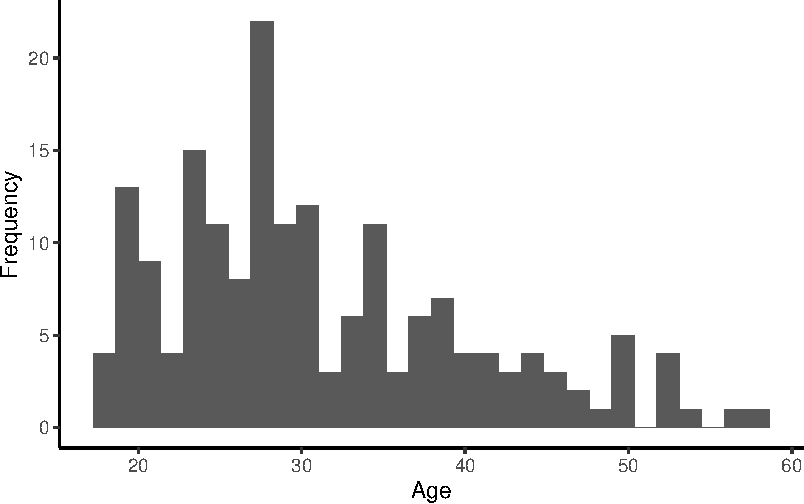
\includegraphics[width=1\textwidth,height=\textheight]{17-analysis-journey-1_files/figure-pdf/unnamed-chunk-21-1.pdf}
\end{center}

\begin{tcolorbox}[enhanced jigsaw, breakable, colframe=quarto-callout-caution-color-frame, arc=.35mm, opacitybacktitle=0.6, titlerule=0mm, colbacktitle=quarto-callout-caution-color!10!white, colback=white, toprule=.15mm, bottomtitle=1mm, toptitle=1mm, title=\textcolor{quarto-callout-caution-color}{\faFire}\hspace{0.5em}{Show me the solution}, bottomrule=.15mm, rightrule=.15mm, leftrule=.75mm, coltitle=black, left=2mm, opacityback=0]

\begin{Shaded}
\begin{Highlighting}[]
\NormalTok{full\_data }\SpecialCharTok{\%\textgreater{}\%} 
  \FunctionTok{ggplot}\NormalTok{(}\FunctionTok{aes}\NormalTok{(}\AttributeTok{x =}\NormalTok{ age)) }\SpecialCharTok{+} 
  \FunctionTok{geom\_histogram}\NormalTok{() }\SpecialCharTok{+} 
  \FunctionTok{scale\_x\_continuous}\NormalTok{(}\AttributeTok{name =} \StringTok{"Age"}\NormalTok{) }\SpecialCharTok{+} 
  \FunctionTok{scale\_y\_continuous}\NormalTok{(}\AttributeTok{name =} \StringTok{"Frequency"}\NormalTok{) }\SpecialCharTok{+} 
  \FunctionTok{theme\_classic}\NormalTok{()}
\end{Highlighting}
\end{Shaded}

\end{tcolorbox}

\begin{enumerate}
\def\labelenumi{\arabic{enumi}.}
\setcounter{enumi}{3}
\tightlist
\item
  A bar plot of the gender breakdown of the sample would look like:
\end{enumerate}

\begin{center}
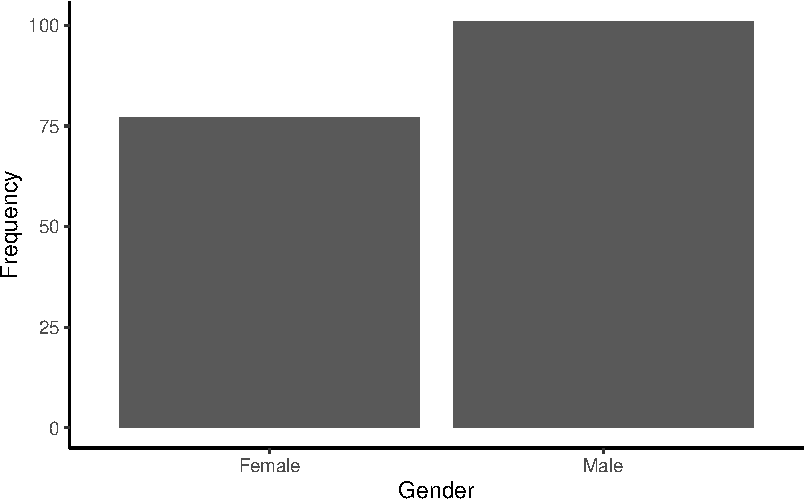
\includegraphics[width=1\textwidth,height=\textheight]{17-analysis-journey-1_files/figure-pdf/unnamed-chunk-23-1.pdf}
\end{center}

\begin{tcolorbox}[enhanced jigsaw, breakable, colframe=quarto-callout-caution-color-frame, arc=.35mm, opacitybacktitle=0.6, titlerule=0mm, colbacktitle=quarto-callout-caution-color!10!white, colback=white, toprule=.15mm, bottomtitle=1mm, toptitle=1mm, title=\textcolor{quarto-callout-caution-color}{\faFire}\hspace{0.5em}{Show me the solution}, bottomrule=.15mm, rightrule=.15mm, leftrule=.75mm, coltitle=black, left=2mm, opacityback=0]

\begin{Shaded}
\begin{Highlighting}[]
\NormalTok{full\_data }\SpecialCharTok{\%\textgreater{}\%} 
  \FunctionTok{ggplot}\NormalTok{(}\FunctionTok{aes}\NormalTok{(}\AttributeTok{x =}\NormalTok{ gender)) }\SpecialCharTok{+} 
  \FunctionTok{geom\_bar}\NormalTok{() }\SpecialCharTok{+}
  \FunctionTok{scale\_x\_discrete}\NormalTok{(}\AttributeTok{name =} \StringTok{"Gender"}\NormalTok{) }\SpecialCharTok{+} 
  \FunctionTok{scale\_y\_continuous}\NormalTok{(}\AttributeTok{name =} \StringTok{"Frequency"}\NormalTok{) }\SpecialCharTok{+} 
  \FunctionTok{theme\_classic}\NormalTok{()}
\end{Highlighting}
\end{Shaded}

\end{tcolorbox}

\subsection{Measures of smoking
dependence}\label{measures-of-smoking-dependence}

\begin{enumerate}
\def\labelenumi{\arabic{enumi}.}
\setcounter{enumi}{4}
\tightlist
\item
  To 2 decimal places, for daily smokers the mean number of cigarettes
  per day was \_\_\_\_ (\emph{SD} = \_\_\_\_) and for non-daily smokers
  the mean number of cigarettes per day was \_\_\_\_ (\emph{SD} =
  \_\_\_\_).
\end{enumerate}

\begin{tcolorbox}[enhanced jigsaw, breakable, colframe=quarto-callout-caution-color-frame, arc=.35mm, opacitybacktitle=0.6, titlerule=0mm, colbacktitle=quarto-callout-caution-color!10!white, colback=white, toprule=.15mm, bottomtitle=1mm, toptitle=1mm, title=\textcolor{quarto-callout-caution-color}{\faFire}\hspace{0.5em}{Show me the solution}, bottomrule=.15mm, rightrule=.15mm, leftrule=.75mm, coltitle=black, left=2mm, opacityback=0]

\begin{Shaded}
\begin{Highlighting}[]
\NormalTok{full\_data }\SpecialCharTok{\%\textgreater{}\%} 
  \FunctionTok{group\_by}\NormalTok{(daily\_smoker) }\SpecialCharTok{\%\textgreater{}\%} 
  \FunctionTok{summarise}\NormalTok{(}\AttributeTok{mean\_cpd =} \FunctionTok{round}\NormalTok{(}\FunctionTok{mean}\NormalTok{(cpd, }\AttributeTok{na.rm =} \ConstantTok{TRUE}\NormalTok{), }\DecValTok{2}\NormalTok{),}
            \AttributeTok{sd\_cpd =} \FunctionTok{round}\NormalTok{(}\FunctionTok{sd}\NormalTok{(cpd, }\AttributeTok{na.rm =} \ConstantTok{TRUE}\NormalTok{), }\DecValTok{2}\NormalTok{))}
\end{Highlighting}
\end{Shaded}

\begin{verbatim}
# A tibble: 2 x 3
  daily_smoker     mean_cpd sd_cpd
  <fct>               <dbl>  <dbl>
1 Daily Smoker         8.85   6.51
2 Non-daily Smoker     2.32   2.69
\end{verbatim}

\end{tcolorbox}

\begin{enumerate}
\def\labelenumi{\arabic{enumi}.}
\setcounter{enumi}{5}
\tightlist
\item
  To 2 decimal places, for daily smokers the mean FTND sum score was
  \_\_\_\_ (\emph{SD} = \textbf{\emph{) and for non-daily smokers the
  mean number of cigarettes per day was }}\_ (\emph{SD} = \_\_\_\_).
\end{enumerate}

\begin{tcolorbox}[enhanced jigsaw, breakable, colframe=quarto-callout-caution-color-frame, arc=.35mm, opacitybacktitle=0.6, titlerule=0mm, colbacktitle=quarto-callout-caution-color!10!white, colback=white, toprule=.15mm, bottomtitle=1mm, toptitle=1mm, title=\textcolor{quarto-callout-caution-color}{\faFire}\hspace{0.5em}{Show me the solution}, bottomrule=.15mm, rightrule=.15mm, leftrule=.75mm, coltitle=black, left=2mm, opacityback=0]

\begin{Shaded}
\begin{Highlighting}[]
\NormalTok{full\_data }\SpecialCharTok{\%\textgreater{}\%} 
  \FunctionTok{group\_by}\NormalTok{(daily\_smoker) }\SpecialCharTok{\%\textgreater{}\%} 
  \FunctionTok{summarise}\NormalTok{(}\AttributeTok{mean\_FTND =} \FunctionTok{round}\NormalTok{(}\FunctionTok{mean}\NormalTok{(FTND\_sum, }\AttributeTok{na.rm =} \ConstantTok{TRUE}\NormalTok{), }\DecValTok{2}\NormalTok{),}
            \AttributeTok{sd\_FTND =} \FunctionTok{round}\NormalTok{(}\FunctionTok{sd}\NormalTok{(FTND\_sum, }\AttributeTok{na.rm =} \ConstantTok{TRUE}\NormalTok{), }\DecValTok{2}\NormalTok{))}
\end{Highlighting}
\end{Shaded}

\begin{verbatim}
# A tibble: 2 x 3
  daily_smoker     mean_FTND sd_FTND
  <fct>                <dbl>   <dbl>
1 Daily Smoker          2.61    2.2 
2 Non-daily Smoker      0.49    1.28
\end{verbatim}

\end{tcolorbox}

\subsection{Attentional bias}\label{attentional-bias}

\begin{enumerate}
\def\labelenumi{\arabic{enumi}.}
\setcounter{enumi}{6}
\item
  Before answering the following questions, complete one extra data
  wrangling step to create difference scores where positive values mean
  attentional bias towards smoking images (faster responses to smoking
  compared to non-smoking stimuli):

  \begin{itemize}
  \item
    Create a new variable called \texttt{difference\_200} by calculating
    \texttt{nonsmoking200} - \texttt{smoking200}.
  \item
    Create a new variable called \texttt{difference\_500} by by
    calculating \texttt{nonsmoking500} - \texttt{smoking500}.
  \end{itemize}
\end{enumerate}

\begin{tcolorbox}[enhanced jigsaw, breakable, colframe=quarto-callout-caution-color-frame, arc=.35mm, opacitybacktitle=0.6, titlerule=0mm, colbacktitle=quarto-callout-caution-color!10!white, colback=white, toprule=.15mm, bottomtitle=1mm, toptitle=1mm, title=\textcolor{quarto-callout-caution-color}{\faFire}\hspace{0.5em}{Show me the solution}, bottomrule=.15mm, rightrule=.15mm, leftrule=.75mm, coltitle=black, left=2mm, opacityback=0]

\begin{Shaded}
\begin{Highlighting}[]
\NormalTok{full\_data }\OtherTok{\textless{}{-}}\NormalTok{ full\_data }\SpecialCharTok{\%\textgreater{}\%} 
  \FunctionTok{mutate}\NormalTok{(}\AttributeTok{difference\_200 =}\NormalTok{ nonsmoking200 }\SpecialCharTok{{-}}\NormalTok{ smoking200,}
         \AttributeTok{difference\_500 =}\NormalTok{ nonsmoking500 }\SpecialCharTok{{-}}\NormalTok{ smoking500)}
\end{Highlighting}
\end{Shaded}

\end{tcolorbox}

\begin{enumerate}
\def\labelenumi{\arabic{enumi}.}
\setcounter{enumi}{7}
\tightlist
\item
  To 2 decimal places, the mean difference in attentional bias in the
  200ms condition was \_\_\_\_ (\emph{SD} = \_\_\_\_\_) for daily
  smokers and \_\_\_\_\_ (\emph{SD} = \_\_\_\_\_) for non-daily smokers.
\end{enumerate}

\begin{tcolorbox}[enhanced jigsaw, breakable, colframe=quarto-callout-caution-color-frame, arc=.35mm, opacitybacktitle=0.6, titlerule=0mm, colbacktitle=quarto-callout-caution-color!10!white, colback=white, toprule=.15mm, bottomtitle=1mm, toptitle=1mm, title=\textcolor{quarto-callout-caution-color}{\faFire}\hspace{0.5em}{Show me the solution}, bottomrule=.15mm, rightrule=.15mm, leftrule=.75mm, coltitle=black, left=2mm, opacityback=0]

\begin{Shaded}
\begin{Highlighting}[]
\NormalTok{full\_data }\SpecialCharTok{\%\textgreater{}\%} 
  \FunctionTok{group\_by}\NormalTok{(daily\_smoker) }\SpecialCharTok{\%\textgreater{}\%} 
  \FunctionTok{summarise}\NormalTok{(}\AttributeTok{mean\_bias\_200 =} \FunctionTok{round}\NormalTok{(}\FunctionTok{mean}\NormalTok{(difference\_200, }\AttributeTok{na.rm =} \ConstantTok{TRUE}\NormalTok{), }\DecValTok{2}\NormalTok{),}
            \AttributeTok{sd\_bias\_200 =} \FunctionTok{round}\NormalTok{(}\FunctionTok{sd}\NormalTok{(difference\_200, }\AttributeTok{na.rm =} \ConstantTok{TRUE}\NormalTok{), }\DecValTok{2}\NormalTok{))}
\end{Highlighting}
\end{Shaded}

\begin{verbatim}
# A tibble: 2 x 3
  daily_smoker     mean_bias_200 sd_bias_200
  <fct>                    <dbl>       <dbl>
1 Daily Smoker              1.25        23.9
2 Non-daily Smoker         -2.74        21.3
\end{verbatim}

\end{tcolorbox}

\begin{enumerate}
\def\labelenumi{\arabic{enumi}.}
\setcounter{enumi}{8}
\tightlist
\item
  To 2 decimal places, the mean difference in attentional bias in the
  500ms condition was \_\_\_\_ (\emph{SD} = \_\_\_\_\_) for daily
  smokers and \_\_\_\_\_ (\emph{SD} = \_\_\_\_\_) for non-daily smokers.
\end{enumerate}

\begin{tcolorbox}[enhanced jigsaw, breakable, colframe=quarto-callout-caution-color-frame, arc=.35mm, opacitybacktitle=0.6, titlerule=0mm, colbacktitle=quarto-callout-caution-color!10!white, colback=white, toprule=.15mm, bottomtitle=1mm, toptitle=1mm, title=\textcolor{quarto-callout-caution-color}{\faFire}\hspace{0.5em}{Show me the solution}, bottomrule=.15mm, rightrule=.15mm, leftrule=.75mm, coltitle=black, left=2mm, opacityback=0]

\begin{Shaded}
\begin{Highlighting}[]
\NormalTok{full\_data }\SpecialCharTok{\%\textgreater{}\%} 
  \FunctionTok{group\_by}\NormalTok{(daily\_smoker) }\SpecialCharTok{\%\textgreater{}\%} 
  \FunctionTok{summarise}\NormalTok{(}\AttributeTok{mean\_bias\_500 =} \FunctionTok{round}\NormalTok{(}\FunctionTok{mean}\NormalTok{(difference\_500, }\AttributeTok{na.rm =} \ConstantTok{TRUE}\NormalTok{), }\DecValTok{2}\NormalTok{),}
            \AttributeTok{sd\_bias\_500 =} \FunctionTok{round}\NormalTok{(}\FunctionTok{sd}\NormalTok{(difference\_500, }\AttributeTok{na.rm =} \ConstantTok{TRUE}\NormalTok{), }\DecValTok{2}\NormalTok{))}
\end{Highlighting}
\end{Shaded}

\begin{verbatim}
# A tibble: 2 x 3
  daily_smoker     mean_bias_500 sd_bias_500
  <fct>                    <dbl>       <dbl>
1 Daily Smoker              0.76        21.7
2 Non-daily Smoker         -1.19        14.5
\end{verbatim}

\end{tcolorbox}

If you are currently completing this after Chapter 6, we have not
covered visualising continuous data or inferential statistics yet. Try
coming back to these tasks to compare these measures when you have
finished Chapter 7 for more advanced visualisation and Chapter 13 for
factorial ANOVA.

A difference score of 0 means no bias towards smoking or non-smoking
images. So, you can see the paper did not find either group showed much
attentional bias towards smoking images nor much difference between the
groups, hence why it was published in the \emph{Journal of Trial and
Error}.

\section{Conclusion}\label{conclusion}

Well done! Hopefully you recognised how far your skills have come to be
able to do this independently, regardless of how many hints you needed.

These are real skills people use in research. If you are curious, J. E.
Bartlett et al. (2022) shared their code as a reproducible manuscrupt,
so you can see all the wrangling steps they completed by looking at
\href{https://osf.io/xpgt3}{this file on the Open Science Framework}. We
did not include all of them here as there are concepts like outliers we
had not covered by Chapter 6.

\bookmarksetup{startatroot}

\chapter{Analysis Journey 2: Simple Linear
Regression}\label{journey-02-wrangling}

Welcome to the second data analysis journey. We have designed these
chapters as a bridge between the structured learning in the core
chapters and your assessments. We present you with a new data set, show
you what the end product should look like, and see if you can apply your
data wrangling, visualisation, and/or analysis skills to get there.

As you gain independence, this is the crucial skill. Data analysis is
all about seeing the data you have available to you and identifying what
the end product needs to be to apply your visualisation and analysis
techniques. You can then mentally (or physically) create a checklist of
tasks to work backwards to get there. There might be a lot of trial and
error as you try one thing, it does not quite work, so you go back and
try something else. If you get stuck though, we have a range of hints
and task lists you can unhide, then the solution to check your attempts
against.

In this second data analysis journey, we focus on inferential statistics
after some data wrangling to apply all the skills you developed from
Chapter 1 to Chapter 9.

\section{Task preparation}\label{task-preparation-1}

\subsection{Introduction to the data
set}\label{introduction-to-the-data-set-11}

For this task, we are using open data from Binfet et al. (2022), where
the authors used the data set to write a separate article on repurposing
it for statistics education (Evans et al., 2023), inspiring us to use it
in the chapter here. The abstract of their article is:

\begin{quote}
Researchers have claimed that canine-assisted interventions (CAIs)
contribute significantly to bolstering participants' wellbeing, yet the
mechanisms within interactions have received little empirical attention.
The aim of this study was to assess the impact of client--canine contact
on wellbeing outcomes in a sample of 284 undergraduate college students
(77\% female; 21\% male, 2\% non-binary). Participants self-selected to
participate and were randomly assigned to one of two canine interaction
treatment conditions (touch or no touch) or to a handler-only condition
with no therapy dog present. To assess self-reports of wellbeing,
measures of flourishing, positive and negative affect, social
connectedness, happiness, integration into the campus community, stress,
homesickness, and loneliness were administered. Exploratory analyses
were conducted to assess whether these wellbeing measures could be
considered as measuring a unidimensional construct. This included both
reliability analysis and exploratory factor analysis. Based on the
results of these analyses we created a composite measure using
participant scores on a latent factor. We then conducted the tests of
the four hypotheses using these factor scores. Results indicate that
participants across all conditions experienced enhanced wellbeing on
several measures; however, only those in the direct contact condition
reported significant improvements on all measures of wellbeing.
Additionally, direct interactions with therapy dogs through touch
elicited greater wellbeing benefits than did no touch/indirect
interactions or interactions with only a dog handler. Similarly,
analyses using scores on the wellbeing factor indicated significant
improvement in wellbeing across all conditions (handler-only,
\emph{d}=0.18, \emph{p}=0.041; indirect, \emph{d}=0.38,
\emph{p}\textless0.001; direct, \emph{d}=0.78, \emph{p}\textless0.001),
with more benefit when a dog was present (\emph{d}=0.20,
\emph{p}\textless0.001), and the most benefit coming from physical
contact with the dog (\emph{d}=0.13, \emph{p}=0.002). The findings hold
implications for post-secondary wellbeing programs as well as the
organization and delivery of CAIs.
\end{quote}

In summary, they were interested in the effect of therapy dogs on
well-being in undergraduate students. Participants were randomly
allocated to one of three groups:

\begin{enumerate}
\def\labelenumi{\arabic{enumi}.}
\item
  Canine interaction touching the dogs (Direct).
\item
  Canine interaction not touching the dogs (Indirect).
\item
  Handler-only with no dogs present (Control).
\end{enumerate}

They measured 9 outcomes before and after the intervention including
social connectedness, stress, and loneliness. For this journey chapter,
we will focus on a constrained set of variables and analyses so it does
not take forever, but the process would apply to all the outcomes. The
authors posed three hypotheses which we will test after some data
wrangling:

\begin{enumerate}
\def\labelenumi{\arabic{enumi}.}
\item
  All treatment groups would have significantly higher measures of
  well-being and lower measures of ill-being after treatment.
\item
  The treatment groups that interact with dogs would have significantly
  higher measures of well-being and lower measures of ill-being compared
  to the handler-only treatment.
\item
  Direct contact with a therapy dog would yield greater benefits than
  indirect contact treatment.
\end{enumerate}

\subsection{Organising your files and project for the
task}\label{organising-your-files-and-project-for-the-task-1}

Before we can get started, you need to organise your files and project
for the task, so your working directory is in order.

\begin{enumerate}
\def\labelenumi{\arabic{enumi}.}
\item
  In your folder for research methods and the book
  \texttt{ResearchMethods1\_2/Quant\_Fundamentals}, create a new folder
  for the data analysis journey called \texttt{Journey\_02\_regression}.
  Within \texttt{Journey\_02\_regression}, create two new folders called
  \texttt{data} and \texttt{figures}.
\item
  Create an R Project for \texttt{Journey\_02\_regression} as an
  existing directory for your chapter folder. This should now be your
  working directory.
\item
  Create a new R Markdown document and give it a sensible title
  describing the chapter, such as
  \texttt{Analysis\ Journey\ 2\ -\ Simple\ Linear\ Regression}. Delete
  everything below line 10 so you have a blank file to work with and
  save the file in your \texttt{Journey\_02\_regression} folder.
\item
  We are working with a new data set, so please save the following data
  file: \href{data/Evans_2023_raw.csv}{Evans\_2023\_raw.csv}. Right
  click the link and select ``save link as'', or clicking the link will
  save the files to your Downloads. Make sure that you save the file as
  ``.csv''. Save or copy the file to your \texttt{data/} folder within
  \texttt{Journey\_02\_regression}.
\end{enumerate}

You are now ready to start working on the task!

\section{Overview}\label{overview-2}

\subsection{Load tidyverse and read the data
file}\label{load-tidyverse-and-read-the-data-file}

Before we explore what wrangling we need to do, complete the following
task list and check the solution if you are stuck.

\begin{tcolorbox}[enhanced jigsaw, breakable, colframe=quarto-callout-tip-color-frame, arc=.35mm, opacitybacktitle=0.6, titlerule=0mm, colbacktitle=quarto-callout-tip-color!10!white, colback=white, toprule=.15mm, bottomtitle=1mm, toptitle=1mm, title=\textcolor{quarto-callout-tip-color}{\faLightbulb}\hspace{0.5em}{Try this}, bottomrule=.15mm, rightrule=.15mm, leftrule=.75mm, coltitle=black, left=2mm, opacityback=0]

Complete the following steps:

\begin{enumerate}
\def\labelenumi{\arabic{enumi}.}
\item
  Load the tidyverse package.
\item
  Read the data file \texttt{data/Evans\_2023\_raw.csv} to the object
  name \texttt{evans\_data}.
\end{enumerate}

\end{tcolorbox}

\begin{tcolorbox}[enhanced jigsaw, breakable, colframe=quarto-callout-tip-color-frame, arc=.35mm, opacitybacktitle=0.6, titlerule=0mm, colbacktitle=quarto-callout-tip-color!10!white, colback=white, toprule=.15mm, bottomtitle=1mm, toptitle=1mm, title=\textcolor{quarto-callout-tip-color}{\faLightbulb}\hspace{0.5em}{Show me the solution}, bottomrule=.15mm, rightrule=.15mm, leftrule=.75mm, coltitle=black, left=2mm, opacityback=0]

You should have the following in a code chunk:

\begin{Shaded}
\begin{Highlighting}[]
\CommentTok{\# load the relevant packages}
\FunctionTok{library}\NormalTok{(tidyverse)}

\CommentTok{\# Read the Evans\_2023\_raw.csv file }
\NormalTok{evans\_data }\OtherTok{\textless{}{-}} \FunctionTok{read\_csv}\NormalTok{(}\StringTok{"data/Evans\_2023\_raw.csv"}\NormalTok{)}
\end{Highlighting}
\end{Shaded}

\end{tcolorbox}

\subsection{\texorpdfstring{Explore
\texttt{evans\_data}}{Explore evans\_data}}\label{explore-evans_data}

In \texttt{evans\_data}, we have the participant ID (\texttt{RID}),
several demographic variables, and pre- and post-test items for stress,
loneliness, and social connectedness. There are 88 variables which would
take up loads of space, so we are just showing a preview of the first 20
here. If you use \texttt{glimpse()}, you will see all 88.

\begin{verbatim}
Rows: 284
Columns: 20
$ RID             <dbl> 1, 2, 3, 4, 5, 6, 7, 8, 9, 10, 11, 12, 13, 14, 15, 16,~
$ GroupAssignment <chr> "Control", "Direct", "Indirect", "Control", "Direct", ~
$ Age_Yrs         <dbl> 21, 19, 18, 18, 19, 20, 26, 17, 21, 22, 19, 20, 19, 19~
$ Year_of_Study   <dbl> 3, 1, 1, 1, 1, 2, 2, 1, 3, 4, 2, 2, 2, 2, 3, 1, 1, 1, ~
$ Live_Pets       <dbl> 2, 2, 2, 2, 2, 2, 1, 2, 2, 2, 2, 2, 2, 2, NA, 2, 2, 1,~
$ Consumer_BARK   <dbl> 1, 1, 1, 1, 1, 1, 1, 1, 1, 1, 1, 1, 1, 1, 2, 2, 1, 1, ~
$ S1_1            <dbl> 2, 2, 4, 2, 3, 4, 4, 3, 2, 2, 3, 2, 3, 4, 3, 2, 4, 2, ~
$ L1_1            <dbl> 3, 3, 3, 4, 2, 4, 3, 2, 3, 4, 3, 3, 4, 4, 4, 2, 3, 4, ~
$ L1_2            <dbl> 3, 2, 3, 2, 3, 3, 2, 3, 4, 1, 3, 3, 2, 3, 1, 4, 3, 2, ~
$ L1_3            <dbl> 4, 3, 2, 2, 3, 3, 1, 3, 3, 1, 2, 2, 1, 3, 1, 3, 3, 1, ~
$ L1_4            <dbl> 3, 3, 3, 3, 3, 3, 3, 3, 4, 1, 2, 3, 2, 3, 2, 4, 3, 2, ~
$ L1_5            <dbl> 2, 4, 3, 4, 4, 3, 2, 4, 4, 4, 4, 4, 4, 4, 4, 2, 3, 4, ~
$ L1_6            <dbl> 3, 3, 4, 4, 3, 2, 3, 3, 3, 4, 3, 3, 4, 3, 4, 2, 2, 4, ~
$ L1_7            <dbl> 1, 2, 2, 1, 2, 2, 4, 2, 2, 1, 3, 2, 3, 2, 2, 2, 3, 3, ~
$ L1_8            <dbl> 2, 2, 3, 3, 2, 3, 2, 3, 3, 2, 3, 2, 2, 3, 2, 4, 3, 2, ~
$ L1_9            <dbl> 3, 4, 3, 3, 3, 3, 3, 3, 2, 4, 3, 3, 4, 4, 4, 3, 2, 3, ~
$ L1_10           <dbl> 4, 3, 3, 4, 2, 2, 3, 3, 3, 4, 4, 3, 4, 4, 4, 2, 2, 3, ~
$ L1_11           <dbl> 3, 2, 2, 2, 4, 3, 4, 2, 2, 1, 3, 2, 2, 2, 2, 4, 3, 2, ~
$ L1_12           <dbl> 1, 2, 2, 1, 4, 3, 2, 2, 1, 1, 2, 2, 1, 2, 2, 1, 3, 1, ~
$ L1_13           <dbl> 3, 1, 2, 2, 4, 3, 3, 3, 4, 1, 3, 4, 2, 2, 2, 4, 3, 2, ~
\end{verbatim}

The columns (variables) we have in the data set are:

\begin{longtable}[]{@{}
  >{\centering\arraybackslash}p{(\columnwidth - 4\tabcolsep) * \real{0.1951}}
  >{\raggedright\arraybackslash}p{(\columnwidth - 4\tabcolsep) * \real{0.4146}}
  >{\raggedright\arraybackslash}p{(\columnwidth - 4\tabcolsep) * \real{0.3902}}@{}}
\toprule\noalign{}
\begin{minipage}[b]{\linewidth}\centering
Variable
\end{minipage} & \begin{minipage}[b]{\linewidth}\raggedright
Type
\end{minipage} & \begin{minipage}[b]{\linewidth}\raggedright
Description
\end{minipage} \\
\midrule\noalign{}
\endhead
\bottomrule\noalign{}
\endlastfoot
RID & double & Participant ID number. \\
GroupAssignment & character & Randomly allocated study group: Control,
Indirect, Direct. \\
Age\_Yrs & double & Age in years. \\
Year\_of\_Study & double & Participant's year in college: First (1),
Second (2), Third (3), Fourth (4), Fifth or more (5). \\
Live\_Pets & double & Does the participant have a pet back at home: Pet
back home (1), no pet back home (2). \\
Consumer\_BARK & double & Is the participant a low (1), medium (2), or
high (3) consumer of the BARK program - the therapy dog service. \\
S1\_1 & double & Stress scale pre-test, 1 item, 1 (not at all stressed)
to 5 (very stressed). \\
L1\_1 to L1\_20 & double & Loneliness scale pre-test, 20 items, 1
(never) to 4 (often). \\
SC1\_1 to SC1\_20 & double & Social connectedness scale pre-test, 20
items, 1 (strongly disagree) to 6 (strongly agree). \\
S2\_1 & double & Stress scale post-test, 1 item. \\
L2\_1 to L2\_20 & double & Loneliness scale post-test, 20 items. \\
SC2\_1 to SC2\_20 & double & Social connectedness scale post-test, 20
items, 1 (strongly disagree) to 6 (strongly agree). \\
\end{longtable}

\begin{tcolorbox}[enhanced jigsaw, breakable, colframe=quarto-callout-tip-color-frame, arc=.35mm, opacitybacktitle=0.6, titlerule=0mm, colbacktitle=quarto-callout-tip-color!10!white, colback=white, toprule=.15mm, bottomtitle=1mm, toptitle=1mm, title=\textcolor{quarto-callout-tip-color}{\faLightbulb}\hspace{0.5em}{Try this}, bottomrule=.15mm, rightrule=.15mm, leftrule=.75mm, coltitle=black, left=2mm, opacityback=0]

Now we have introduced the data set, explore them using different
methods we introduced. For example, opening the data object as a tab to
scroll around, explore with \texttt{glimpse()}, or even try plotting
some of the individual variables to see what they look like.

\end{tcolorbox}

\section{Wrangling}\label{wrangling}

We are going to show you a preview of the starting data set and the end
product we are aiming for. For the raw data, we have limited this to the
first 20 rows again just so it does not take up the whole page, but if
you use \texttt{glimpse()} you will see all 88 variables.

\subsubsection{Raw data}

\begin{verbatim}
Rows: 284
Columns: 20
$ RID             <dbl> 1, 2, 3, 4, 5, 6, 7, 8, 9, 10, 11, 12, 13, 14, 15, 16,~
$ GroupAssignment <chr> "Control", "Direct", "Indirect", "Control", "Direct", ~
$ Age_Yrs         <dbl> 21, 19, 18, 18, 19, 20, 26, 17, 21, 22, 19, 20, 19, 19~
$ Year_of_Study   <dbl> 3, 1, 1, 1, 1, 2, 2, 1, 3, 4, 2, 2, 2, 2, 3, 1, 1, 1, ~
$ Live_Pets       <dbl> 2, 2, 2, 2, 2, 2, 1, 2, 2, 2, 2, 2, 2, 2, NA, 2, 2, 1,~
$ Consumer_BARK   <dbl> 1, 1, 1, 1, 1, 1, 1, 1, 1, 1, 1, 1, 1, 1, 2, 2, 1, 1, ~
$ S1_1            <dbl> 2, 2, 4, 2, 3, 4, 4, 3, 2, 2, 3, 2, 3, 4, 3, 2, 4, 2, ~
$ L1_1            <dbl> 3, 3, 3, 4, 2, 4, 3, 2, 3, 4, 3, 3, 4, 4, 4, 2, 3, 4, ~
$ L1_2            <dbl> 3, 2, 3, 2, 3, 3, 2, 3, 4, 1, 3, 3, 2, 3, 1, 4, 3, 2, ~
$ L1_3            <dbl> 4, 3, 2, 2, 3, 3, 1, 3, 3, 1, 2, 2, 1, 3, 1, 3, 3, 1, ~
$ L1_4            <dbl> 3, 3, 3, 3, 3, 3, 3, 3, 4, 1, 2, 3, 2, 3, 2, 4, 3, 2, ~
$ L1_5            <dbl> 2, 4, 3, 4, 4, 3, 2, 4, 4, 4, 4, 4, 4, 4, 4, 2, 3, 4, ~
$ L1_6            <dbl> 3, 3, 4, 4, 3, 2, 3, 3, 3, 4, 3, 3, 4, 3, 4, 2, 2, 4, ~
$ L1_7            <dbl> 1, 2, 2, 1, 2, 2, 4, 2, 2, 1, 3, 2, 3, 2, 2, 2, 3, 3, ~
$ L1_8            <dbl> 2, 2, 3, 3, 2, 3, 2, 3, 3, 2, 3, 2, 2, 3, 2, 4, 3, 2, ~
$ L1_9            <dbl> 3, 4, 3, 3, 3, 3, 3, 3, 2, 4, 3, 3, 4, 4, 4, 3, 2, 3, ~
$ L1_10           <dbl> 4, 3, 3, 4, 2, 2, 3, 3, 3, 4, 4, 3, 4, 4, 4, 2, 2, 3, ~
$ L1_11           <dbl> 3, 2, 2, 2, 4, 3, 4, 2, 2, 1, 3, 2, 2, 2, 2, 4, 3, 2, ~
$ L1_12           <dbl> 1, 2, 2, 1, 4, 3, 2, 2, 1, 1, 2, 2, 1, 2, 2, 1, 3, 1, ~
$ L1_13           <dbl> 3, 1, 2, 2, 4, 3, 3, 3, 4, 1, 3, 4, 2, 2, 2, 4, 3, 2, ~
\end{verbatim}

\subsubsection{Wrangled data}

\begin{verbatim}
Rows: 284
Columns: 12
$ RID             <dbl> 1, 2, 3, 4, 5, 6, 7, 8, 9, 10, 11, 12, 13, 14, 15, 16,~
$ GroupAssignment <chr> "Control", "Direct", "Indirect", "Control", "Direct", ~
$ Age_Yrs         <dbl> 21, 19, 18, 18, 19, 20, 26, 17, 21, 22, 19, 20, 19, 19~
$ Year_of_Study   <dbl> 3, 1, 1, 1, 1, 2, 2, 1, 3, 4, 2, 2, 2, 2, 3, 1, 1, 1, ~
$ Live_Pets       <chr> "Does not have a pet back home", "Does not have a pet ~
$ Consumer_BARK   <chr> "Low", "Low", "Low", "Low", "Low", "Low", "Low", "Low"~
$ stress_pre      <dbl> 2, 2, 4, 2, 3, 4, 4, 3, 2, 2, 3, 2, 3, 4, 3, 2, 4, 2, ~
$ stress_post     <dbl> 2, 1, 3, 2, 4, 4, 3, 2, 2, 1, 2, 2, 1, 2, 4, 2, 2, 1, ~
$ lonely_pre      <dbl> 2.25, 1.90, 2.25, 1.75, 2.85, 2.70, 2.40, 2.25, 2.55, ~
$ lonely_post     <dbl> 1.70, 1.60, 2.25, 2.05, 2.70, 2.40, 2.25, 2.00, 2.55, ~
$ social_pre      <dbl> 3.90, 5.15, 4.10, 4.65, 3.65, 4.35, 4.75, 4.60, 4.20, ~
$ social_post     <dbl> 3.800000, 5.263158, 4.150000, 5.100000, 3.600000, 4.65~
\end{verbatim}

\begin{tcolorbox}[enhanced jigsaw, breakable, colframe=quarto-callout-tip-color-frame, arc=.35mm, opacitybacktitle=0.6, titlerule=0mm, colbacktitle=quarto-callout-tip-color!10!white, colback=white, toprule=.15mm, bottomtitle=1mm, toptitle=1mm, title=\textcolor{quarto-callout-tip-color}{\faLightbulb}\hspace{0.5em}{Try this}, bottomrule=.15mm, rightrule=.15mm, leftrule=.75mm, coltitle=black, left=2mm, opacityback=0]

Before we give you a task list, try and switch between the raw data and
the wrangled data. Make a list of all the differences you can see
between the two data objects.

\begin{enumerate}
\def\labelenumi{\arabic{enumi}.}
\item
  Do the values of variables change from numbers? How might you recode
  them using the code book above?
\item
  Looking at the codebook, are some variables the same but renamed?
\item
  Looking at the codebook, have we calculated the mean of all the items
  for a scale?
\end{enumerate}

Try and wrangle the data based on all the differences you notice to
create a new object \texttt{evans\_wide}.

For one hint, unless you read the original paper, there are a bunch of
items that first need reverse coding you would not know about:

\begin{itemize}
\item
  Loneliness pre-test: L1\_1, L1\_5, L1\_6, L1\_9, L1\_10, L1\_15,
  L1\_16, L1\_19, L1\_20.
\item
  Loneliness post-test: L2\_1, L2\_5, L2\_6, L2\_9, L2\_10, L2\_15,
  L2\_16, L2\_19, L2\_20.
\item
  Social connectedness pre-test: SC1\_3, SC1\_6, SC1\_7, SC1\_9,
  SC1\_11, SC1\_13, SC1\_15, SC1\_17, SC1\_18, SC1\_20.
\item
  Social connectedness post-test: SC2\_3, SC2\_6, SC2\_7, SC2\_9,
  SC2\_11, SC2\_13, SC2\_15, SC2\_17, SC2\_18, SC2\_20.
\end{itemize}

When you get as far as you can, check the task list which explains all
the steps we applied, but not how to do them. Then, you can check the
solution for our code.

\end{tcolorbox}

\subsection{Task list}\label{task-list-3}

\begin{tcolorbox}[enhanced jigsaw, breakable, colframe=quarto-callout-note-color-frame, arc=.35mm, opacitybacktitle=0.6, titlerule=0mm, colbacktitle=quarto-callout-note-color!10!white, colback=white, toprule=.15mm, bottomtitle=1mm, toptitle=1mm, title=\textcolor{quarto-callout-note-color}{\faInfo}\hspace{0.5em}{Show me the task list}, bottomrule=.15mm, rightrule=.15mm, leftrule=.75mm, coltitle=black, left=2mm, opacityback=0]

These are all the steps we applied to create the wrangled data object:

\begin{enumerate}
\def\labelenumi{\arabic{enumi}.}
\item
  Recode \texttt{Live\_Pets} to the two labels outlined in the code
  book.
\item
  Recode \texttt{Consumer\_BARK} to the three labels outlined in the
  code book.
\item
  Reverse code the loneliness and social connectedness items outlined
  above. Think of previous examples where we explained reverse coding
  for how you can do this efficiently.
\end{enumerate}

As one extra piece of advice if you do not want to recode 40 variables
one by one, there is a more advanced function you can use within
\texttt{mutate()}. The function \texttt{across()} lets you apply a
function or calculation to several columns at once. For example, if we
wanted to reverse score items on a 4-point scale, it would look like the
following:

\begin{Shaded}
\begin{Highlighting}[]
\FunctionTok{mutate}\NormalTok{(}\FunctionTok{across}\NormalTok{(}\AttributeTok{.cols =} \FunctionTok{c}\NormalTok{(column1, column2...), }
              \AttributeTok{.fns =} \SpecialCharTok{\textasciitilde{}} \DecValTok{5} \SpecialCharTok{{-}}\NormalTok{ .x))}
\end{Highlighting}
\end{Shaded}

In \texttt{.cols}, we enter all the columns we want to apply the
function to.

In \texttt{.fns} after the \texttt{=}, we add the function we want to
apply to all the columns we selected. The code is a little awkward as we
have a tilde \texttt{\textasciitilde{}}, here the calculation we want to
apply, and \texttt{.x} in place of the column name. You could summarise
it as: for all the columns I select, subtract each value from 5. Once
you get used to the format, \texttt{across()} is really helpful when you
want to do the same thing to multiple columns.

\begin{enumerate}
\def\labelenumi{\arabic{enumi}.}
\setcounter{enumi}{3}
\item
  After reverse coding the items, calculate the subscale mean scores for
  loneliness and social connectedness. You must do this twice per scale,
  as we have the 20 items for the pre-test and 20 items for the
  post-test per scale.
\item
  If you calculated the subscale mean scores individually, join them
  back to the \texttt{evans\_clean} object you mutated.
\item
  Select the following columns:

  \begin{itemize}
  \item
    \texttt{RID} to \texttt{Consumer\_BARK}.
  \item
    Rename \texttt{S1\_1} to \texttt{stress\_pre}.
  \item
    Rename \texttt{S2\_1} to \texttt{stress\_post}.
  \item
    Select your four subscale mean score variables.
  \end{itemize}
\end{enumerate}

Remember: If it's easier for you to complete steps with longer but
accurate code, there is nothing wrong with that. You recognise ways to
make your code more efficient over time.

\end{tcolorbox}

\subsection{Solution}\label{solution-20}

\begin{tcolorbox}[enhanced jigsaw, breakable, colframe=quarto-callout-caution-color-frame, arc=.35mm, opacitybacktitle=0.6, titlerule=0mm, colbacktitle=quarto-callout-caution-color!10!white, colback=white, toprule=.15mm, bottomtitle=1mm, toptitle=1mm, title=\textcolor{quarto-callout-caution-color}{\faFire}\hspace{0.5em}{Show me the solution}, bottomrule=.15mm, rightrule=.15mm, leftrule=.75mm, coltitle=black, left=2mm, opacityback=0]

This is the code we used to create the new object \texttt{evans\_wide}
using the original object \texttt{evans\_data}. As long as you get the
same end result, the exact code is not important. In coding, there are
multiple ways of getting to the same end result. Maybe you found a more
efficient way to complete some of the steps compared to us. Maybe your
code was a little longer. As long as it worked, that is the most
important thing.

\begin{Shaded}
\begin{Highlighting}[]
\CommentTok{\# Initial cleaning step to recode pets and BARK}
\CommentTok{\# then reverse code a bunch of items }
\NormalTok{evans\_clean }\OtherTok{\textless{}{-}}\NormalTok{ evans\_data }\SpecialCharTok{\%\textgreater{}\%} 
  \FunctionTok{mutate}\NormalTok{(}\AttributeTok{Live\_Pets =} \FunctionTok{case\_match}\NormalTok{(Live\_Pets,}
                                \DecValTok{1} \SpecialCharTok{\textasciitilde{}} \StringTok{"Has a pet back home"}\NormalTok{,}
                                \DecValTok{2} \SpecialCharTok{\textasciitilde{}} \StringTok{"Does not have a pet back home"}\NormalTok{),}
         \AttributeTok{Consumer\_BARK =} \FunctionTok{case\_match}\NormalTok{(Consumer\_BARK,}
                                    \DecValTok{1} \SpecialCharTok{\textasciitilde{}} \StringTok{"Low"}\NormalTok{,}
                                    \DecValTok{2} \SpecialCharTok{\textasciitilde{}} \StringTok{"Medium"}\NormalTok{,}
                                    \DecValTok{3} \SpecialCharTok{\textasciitilde{}} \StringTok{"High"}\NormalTok{),}
         \CommentTok{\# across works with mutate to apply the same function to several columns}
         \CommentTok{\# So, take all the loneliness items to reverse code, then subtract them from 5}
         \FunctionTok{across}\NormalTok{(}\AttributeTok{.cols =} \FunctionTok{c}\NormalTok{(L1\_1, L1\_5, L1\_6, L1\_9, L1\_10, L1\_15, L1\_16, L1\_19, L1\_20,}
\NormalTok{                          L2\_1, L2\_5, L2\_6, L2\_9, L2\_10, L2\_15, L2\_16, L2\_19, L2\_20),}
                \AttributeTok{.fns =} \SpecialCharTok{\textasciitilde{}} \DecValTok{5} \SpecialCharTok{{-}}\NormalTok{ .x),}
         \CommentTok{\# take all the connectedness items to reverse code, then subtract them from 7}
         \FunctionTok{across}\NormalTok{(}\AttributeTok{.cols =} \FunctionTok{c}\NormalTok{(SC1\_3, SC1\_6, SC1\_7, SC1\_9, SC1\_11, SC1\_13, SC1\_15, SC1\_17, SC1\_18, SC1\_20, }
\NormalTok{                          SC2\_3, SC2\_6, SC2\_7, SC2\_9, SC2\_11, SC2\_13, SC2\_15, SC2\_17, SC2\_18, SC2\_20),}
                \AttributeTok{.fns =} \SpecialCharTok{\textasciitilde{}} \DecValTok{7} \SpecialCharTok{{-}}\NormalTok{ .x))}

\CommentTok{\# There are more elegant ways around this, but for each set, }
\CommentTok{\# take the 20 items, group by participant ID, and calculate the mean, ignoring missing values}
\NormalTok{lonely\_pre }\OtherTok{\textless{}{-}}\NormalTok{ evans\_clean }\SpecialCharTok{\%\textgreater{}\%} 
  \FunctionTok{pivot\_longer}\NormalTok{(}\AttributeTok{cols =}\NormalTok{ L1\_1}\SpecialCharTok{:}\NormalTok{L1\_20, }
               \AttributeTok{names\_to =} \StringTok{"Item"}\NormalTok{, }
               \AttributeTok{values\_to =} \StringTok{"Response"}\NormalTok{) }\SpecialCharTok{\%\textgreater{}\%} 
  \FunctionTok{group\_by}\NormalTok{(RID) }\SpecialCharTok{\%\textgreater{}\%} 
  \FunctionTok{summarise}\NormalTok{(}\AttributeTok{lonely\_pre =} \FunctionTok{mean}\NormalTok{(Response, }\AttributeTok{na.rm =} \ConstantTok{TRUE}\NormalTok{))}

\CommentTok{\# Same thing for post scores}
\NormalTok{lonely\_post }\OtherTok{\textless{}{-}}\NormalTok{ evans\_clean }\SpecialCharTok{\%\textgreater{}\%} 
  \FunctionTok{pivot\_longer}\NormalTok{(}\AttributeTok{cols =}\NormalTok{ L2\_1}\SpecialCharTok{:}\NormalTok{L2\_20, }
               \AttributeTok{names\_to =} \StringTok{"Item"}\NormalTok{, }
               \AttributeTok{values\_to =} \StringTok{"Response"}\NormalTok{) }\SpecialCharTok{\%\textgreater{}\%} 
  \FunctionTok{group\_by}\NormalTok{(RID) }\SpecialCharTok{\%\textgreater{}\%} 
  \FunctionTok{summarise}\NormalTok{(}\AttributeTok{lonely\_post =} \FunctionTok{mean}\NormalTok{(Response, }\AttributeTok{na.rm =} \ConstantTok{TRUE}\NormalTok{))}

\CommentTok{\# take the 20 items, group by participant ID, and calculate the mean, ignoring missing values}
\NormalTok{social\_pre }\OtherTok{\textless{}{-}}\NormalTok{ evans\_clean }\SpecialCharTok{\%\textgreater{}\%} 
  \FunctionTok{pivot\_longer}\NormalTok{(}\AttributeTok{cols =}\NormalTok{ SC1\_1}\SpecialCharTok{:}\NormalTok{SC1\_20, }
               \AttributeTok{names\_to =} \StringTok{"Item"}\NormalTok{, }
               \AttributeTok{values\_to =} \StringTok{"Response"}\NormalTok{) }\SpecialCharTok{\%\textgreater{}\%} 
  \FunctionTok{group\_by}\NormalTok{(RID) }\SpecialCharTok{\%\textgreater{}\%} 
  \FunctionTok{summarise}\NormalTok{(}\AttributeTok{social\_pre =} \FunctionTok{mean}\NormalTok{(Response, }\AttributeTok{na.rm =} \ConstantTok{TRUE}\NormalTok{))}

\CommentTok{\# Same thing for post scores}
\NormalTok{social\_post }\OtherTok{\textless{}{-}}\NormalTok{ evans\_clean }\SpecialCharTok{\%\textgreater{}\%} 
  \FunctionTok{pivot\_longer}\NormalTok{(}\AttributeTok{cols =}\NormalTok{ SC2\_1}\SpecialCharTok{:}\NormalTok{SC2\_20, }
               \AttributeTok{names\_to =} \StringTok{"Item"}\NormalTok{, }
               \AttributeTok{values\_to =} \StringTok{"Response"}\NormalTok{) }\SpecialCharTok{\%\textgreater{}\%} 
  \FunctionTok{group\_by}\NormalTok{(RID) }\SpecialCharTok{\%\textgreater{}\%} 
  \FunctionTok{summarise}\NormalTok{(}\AttributeTok{social\_post =} \FunctionTok{mean}\NormalTok{(Response, }\AttributeTok{na.rm =} \ConstantTok{TRUE}\NormalTok{))}

\CommentTok{\# join all four summary values to main data}
\CommentTok{\# select just the key variables we need}
\CommentTok{\# rename the two stress items}
\NormalTok{evans\_wide }\OtherTok{\textless{}{-}}\NormalTok{ evans\_clean }\SpecialCharTok{\%\textgreater{}\%} 
  \FunctionTok{inner\_join}\NormalTok{(lonely\_pre) }\SpecialCharTok{\%\textgreater{}\%} 
  \FunctionTok{inner\_join}\NormalTok{(lonely\_post) }\SpecialCharTok{\%\textgreater{}\%} 
  \FunctionTok{inner\_join}\NormalTok{(social\_pre) }\SpecialCharTok{\%\textgreater{}\%} 
  \FunctionTok{inner\_join}\NormalTok{(social\_post) }\SpecialCharTok{\%\textgreater{}\%} 
  \FunctionTok{select}\NormalTok{(RID}\SpecialCharTok{:}\NormalTok{Consumer\_BARK, }
         \AttributeTok{stress\_pre =}\NormalTok{ S1\_1, }
         \AttributeTok{stress\_post =}\NormalTok{ S2\_1, }
\NormalTok{         lonely\_pre}\SpecialCharTok{:}\NormalTok{social\_post)}
\end{Highlighting}
\end{Shaded}

\end{tcolorbox}

\section{Summarising/visualising}\label{summarisingvisualising}

You should now have an object called \texttt{evans\_wide} containing 12
variables. If you struggled completing the wrangling steps, you can copy
the code from the solution to follow along from this point. In this
section, we will calculate some summary statistics and plot the data to
see what we can learn. We present you with a list of questions to answer
using your wrangling and visualisation skills, interspersed with the
solutions to check if you are stuck.

\subsection{Demographics}\label{demographics-1}

For demographics, we will recreate some values from Table 1 from Binfet
et al. (2022).

\begin{enumerate}
\def\labelenumi{\arabic{enumi}.}
\item
  How many participants were in each group for \texttt{GroupAssignment}?

  \begin{itemize}
  \item
    \_\_ Control
  \item
    \_\_ Direct
  \item
    \_\_ Indirect
  \end{itemize}
\end{enumerate}

\begin{tcolorbox}[enhanced jigsaw, breakable, colframe=quarto-callout-caution-color-frame, arc=.35mm, opacitybacktitle=0.6, titlerule=0mm, colbacktitle=quarto-callout-caution-color!10!white, colback=white, toprule=.15mm, bottomtitle=1mm, toptitle=1mm, title=\textcolor{quarto-callout-caution-color}{\faFire}\hspace{0.5em}{Show me the solution}, bottomrule=.15mm, rightrule=.15mm, leftrule=.75mm, coltitle=black, left=2mm, opacityback=0]

This nicely reproduces their values.

\begin{Shaded}
\begin{Highlighting}[]
\NormalTok{evans\_wide }\SpecialCharTok{\%\textgreater{}\%} 
  \FunctionTok{count}\NormalTok{(GroupAssignment)}
\end{Highlighting}
\end{Shaded}

\begin{verbatim}
# A tibble: 3 x 2
  GroupAssignment     n
  <chr>           <int>
1 Control            94
2 Direct             95
3 Indirect           95
\end{verbatim}

\end{tcolorbox}

\begin{enumerate}
\def\labelenumi{\arabic{enumi}.}
\setcounter{enumi}{1}
\item
  To 2 decimals, what was the mean and standard deviation age per group?

  \begin{itemize}
  \item
    Control: \emph{M} = \_\_\_\_\_, \emph{SD} = \_\_\_\_.
  \item
    Direct: \emph{M} = \_\_\_\_\_, \emph{SD} = \_\_\_\_.
  \item
    Indirect: \emph{M} = \_\_\_\_\_, \emph{SD} = \_\_\_\_.
  \end{itemize}
\end{enumerate}

\begin{tcolorbox}[enhanced jigsaw, breakable, colframe=quarto-callout-caution-color-frame, arc=.35mm, opacitybacktitle=0.6, titlerule=0mm, colbacktitle=quarto-callout-caution-color!10!white, colback=white, toprule=.15mm, bottomtitle=1mm, toptitle=1mm, title=\textcolor{quarto-callout-caution-color}{\faFire}\hspace{0.5em}{Show me the solution}, bottomrule=.15mm, rightrule=.15mm, leftrule=.75mm, coltitle=black, left=2mm, opacityback=0]

Weirdly, this reproduces the standard deviations from Table 1, but not
the means.

\begin{Shaded}
\begin{Highlighting}[]
\NormalTok{evans\_wide }\SpecialCharTok{\%\textgreater{}\%} 
  \FunctionTok{group\_by}\NormalTok{(GroupAssignment) }\SpecialCharTok{\%\textgreater{}\%} 
  \FunctionTok{summarise}\NormalTok{(}\AttributeTok{mean\_age =} \FunctionTok{round}\NormalTok{(}\FunctionTok{mean}\NormalTok{(Age\_Yrs), }\DecValTok{2}\NormalTok{),}
            \AttributeTok{sd\_age =} \FunctionTok{round}\NormalTok{(}\FunctionTok{sd}\NormalTok{(Age\_Yrs), }\DecValTok{2}\NormalTok{))}
\end{Highlighting}
\end{Shaded}

\begin{verbatim}
# A tibble: 3 x 3
  GroupAssignment mean_age sd_age
  <chr>              <dbl>  <dbl>
1 Control             20.0   2.89
2 Direct              19.8   1.94
3 Indirect            20.0   2.23
\end{verbatim}

\end{tcolorbox}

\begin{enumerate}
\def\labelenumi{\arabic{enumi}.}
\setcounter{enumi}{2}
\item
  How many participants in each group have a pet at home?

  \begin{itemize}
  \item
    \_\_ Control
  \item
    \_\_ Direct
  \item
    \_\_ Indirect
  \end{itemize}
\end{enumerate}

\begin{tcolorbox}[enhanced jigsaw, breakable, colframe=quarto-callout-caution-color-frame, arc=.35mm, opacitybacktitle=0.6, titlerule=0mm, colbacktitle=quarto-callout-caution-color!10!white, colback=white, toprule=.15mm, bottomtitle=1mm, toptitle=1mm, title=\textcolor{quarto-callout-caution-color}{\faFire}\hspace{0.5em}{Show me the solution}, bottomrule=.15mm, rightrule=.15mm, leftrule=.75mm, coltitle=black, left=2mm, opacityback=0]

This nicely reproduces their values.

\begin{Shaded}
\begin{Highlighting}[]
\NormalTok{evans\_wide }\SpecialCharTok{\%\textgreater{}\%} 
  \FunctionTok{count}\NormalTok{(GroupAssignment, Live\_Pets)}
\end{Highlighting}
\end{Shaded}

\begin{verbatim}
# A tibble: 9 x 3
  GroupAssignment Live_Pets                         n
  <chr>           <chr>                         <int>
1 Control         Does not have a pet back home    72
2 Control         Has a pet back home              21
3 Control         <NA>                              1
4 Direct          Does not have a pet back home    63
5 Direct          Has a pet back home              30
6 Direct          <NA>                              2
7 Indirect        Does not have a pet back home    60
8 Indirect        Has a pet back home              34
9 Indirect        <NA>                              1
\end{verbatim}

\end{tcolorbox}

\begin{enumerate}
\def\labelenumi{\arabic{enumi}.}
\setcounter{enumi}{3}
\tightlist
\item
  This is not part of their article, but one interesting question might
  be how many people have a pet at home (\texttt{Live\_Pets}) against
  how frequently they use the BARK program (\texttt{Consumer\_BARK}).
  Try and recreate the following bar plot to visualise this as close as
  possible. We have intentionally used some features we have not covered
  in the data visualisation chapters to get you problem solving. For one
  hint though, we used option D for the viridis colour scheme.
\end{enumerate}

\begin{center}
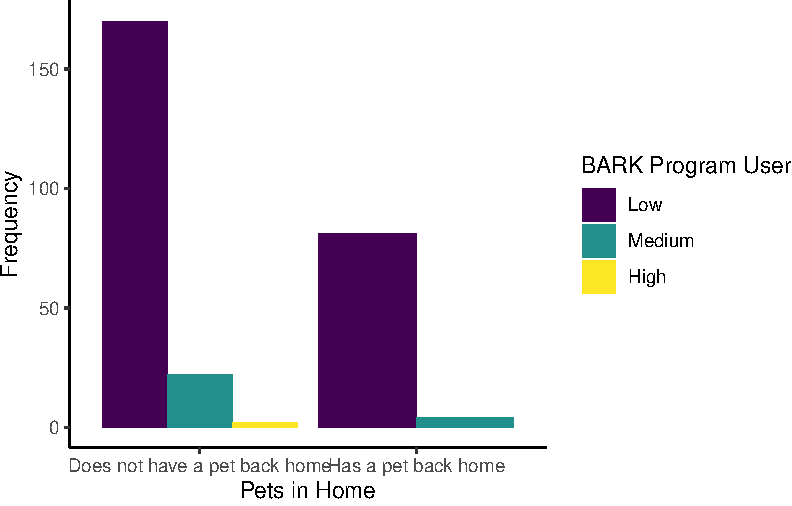
\includegraphics[width=1\textwidth,height=\textheight]{18-analysis-journey-2_files/figure-pdf/unnamed-chunk-11-1.pdf}
\end{center}

\begin{tcolorbox}[enhanced jigsaw, breakable, colframe=quarto-callout-caution-color-frame, arc=.35mm, opacitybacktitle=0.6, titlerule=0mm, colbacktitle=quarto-callout-caution-color!10!white, colback=white, toprule=.15mm, bottomtitle=1mm, toptitle=1mm, title=\textcolor{quarto-callout-caution-color}{\faFire}\hspace{0.5em}{Show me the solution}, bottomrule=.15mm, rightrule=.15mm, leftrule=.75mm, coltitle=black, left=2mm, opacityback=0]

The new features we hoped you found independently were:

\begin{itemize}
\item
  Setting the factor order to show \texttt{Consumer\_BARK} as low,
  medium, then high.
\item
  Set \texttt{position\ =\ "dodge"} to avoid the stacked bar chart.
\item
  Edited the legend title by using the \texttt{name} argument in the
  \texttt{scale\_fill} layer.
\end{itemize}

\begin{Shaded}
\begin{Highlighting}[]
\NormalTok{evans\_wide }\SpecialCharTok{\%\textgreater{}\%} 
  \FunctionTok{drop\_na}\NormalTok{(Live\_Pets, Consumer\_BARK) }\SpecialCharTok{\%\textgreater{}\%} 
  \FunctionTok{mutate}\NormalTok{(}\AttributeTok{Consumer\_BARK =} \FunctionTok{factor}\NormalTok{(Consumer\_BARK, }
                                \AttributeTok{levels =} \FunctionTok{c}\NormalTok{(}\StringTok{"Low"}\NormalTok{, }\StringTok{"Medium"}\NormalTok{, }\StringTok{"High"}\NormalTok{))) }\SpecialCharTok{\%\textgreater{}\%} 
  \FunctionTok{ggplot}\NormalTok{(}\FunctionTok{aes}\NormalTok{(}\AttributeTok{x =}\NormalTok{ Live\_Pets, }\AttributeTok{fill =}\NormalTok{ Consumer\_BARK)) }\SpecialCharTok{+} 
  \FunctionTok{geom\_bar}\NormalTok{(}\AttributeTok{position =} \StringTok{"dodge"}\NormalTok{) }\SpecialCharTok{+} 
  \FunctionTok{labs}\NormalTok{(}\AttributeTok{x =} \StringTok{"Pets in Home"}\NormalTok{, }
       \AttributeTok{y =} \StringTok{"Frequency"}\NormalTok{) }\SpecialCharTok{+} 
  \FunctionTok{scale\_fill\_viridis\_d}\NormalTok{(}\AttributeTok{option =} \StringTok{"D"}\NormalTok{, }
                       \AttributeTok{name =} \StringTok{"BARK Program User"}\NormalTok{) }\SpecialCharTok{+} 
  \FunctionTok{theme\_classic}\NormalTok{()}
\end{Highlighting}
\end{Shaded}

\end{tcolorbox}

\subsection{Wellbeing measures}\label{wellbeing-measures}

For wellbeing and ill-being measures, we will recreate some values from
Table 2 from Binfet et al. (2022).

\begin{enumerate}
\def\labelenumi{\arabic{enumi}.}
\setcounter{enumi}{4}
\item
  If you calculate the mean and standard deviation of each variable per
  group, answer the following questions:

  \begin{itemize}
  \tightlist
  \item
    Which group has the lowest post-test stress value?
  \end{itemize}
\end{enumerate}

\begin{itemize}
\item
  \begin{enumerate}
  \def\labelenumi{(\Alph{enumi})}
  \tightlist
  \item
    Control\\
  \end{enumerate}
\item
  \begin{enumerate}
  \def\labelenumi{(\Alph{enumi})}
  \setcounter{enumi}{1}
  \tightlist
  \item
    Indirect\\
  \end{enumerate}
\item
  \begin{enumerate}
  \def\labelenumi{(\Alph{enumi})}
  \setcounter{enumi}{2}
  \tightlist
  \item
    Direct
  \end{enumerate}

  \begin{itemize}
  \tightlist
  \item
    Which group has the lowest post-test loneliness value?
  \end{itemize}
\item
  \begin{enumerate}
  \def\labelenumi{(\Alph{enumi})}
  \tightlist
  \item
    Control\\
  \end{enumerate}
\item
  \begin{enumerate}
  \def\labelenumi{(\Alph{enumi})}
  \setcounter{enumi}{1}
  \tightlist
  \item
    Direct\\
  \end{enumerate}
\item
  \begin{enumerate}
  \def\labelenumi{(\Alph{enumi})}
  \setcounter{enumi}{2}
  \tightlist
  \item
    Indirect
  \end{enumerate}

  \begin{itemize}
  \tightlist
  \item
    Which group has the lowest post-test social connectedness value?
  \end{itemize}
\item
  \begin{enumerate}
  \def\labelenumi{(\Alph{enumi})}
  \tightlist
  \item
    Direct\\
  \end{enumerate}
\item
  \begin{enumerate}
  \def\labelenumi{(\Alph{enumi})}
  \setcounter{enumi}{1}
  \tightlist
  \item
    Control\\
  \end{enumerate}
\item
  \begin{enumerate}
  \def\labelenumi{(\Alph{enumi})}
  \setcounter{enumi}{2}
  \tightlist
  \item
    Indirect
  \end{enumerate}
\end{itemize}

\begin{tcolorbox}[enhanced jigsaw, breakable, colframe=quarto-callout-caution-color-frame, arc=.35mm, opacitybacktitle=0.6, titlerule=0mm, colbacktitle=quarto-callout-caution-color!10!white, colback=white, toprule=.15mm, bottomtitle=1mm, toptitle=1mm, title=\textcolor{quarto-callout-caution-color}{\faFire}\hspace{0.5em}{Show me the solution}, bottomrule=.15mm, rightrule=.15mm, leftrule=.75mm, coltitle=black, left=2mm, opacityback=0]

This table calculates the mean and standard score for each variable per
group. You can use this to answer the questions above.

\begin{Shaded}
\begin{Highlighting}[]
\NormalTok{evans\_wide }\SpecialCharTok{\%\textgreater{}\%} 
  \FunctionTok{pivot\_longer}\NormalTok{(}\AttributeTok{cols =}\NormalTok{ stress\_pre}\SpecialCharTok{:}\NormalTok{social\_post, }
               \AttributeTok{names\_to =} \StringTok{"Variable"}\NormalTok{, }
               \AttributeTok{values\_to =} \StringTok{"Value"}\NormalTok{) }\SpecialCharTok{\%\textgreater{}\%} 
  \FunctionTok{group\_by}\NormalTok{(GroupAssignment, Variable) }\SpecialCharTok{\%\textgreater{}\%} 
  \FunctionTok{summarise}\NormalTok{(}\AttributeTok{mean\_score =} \FunctionTok{round}\NormalTok{(}\FunctionTok{mean}\NormalTok{(Value), }\DecValTok{2}\NormalTok{), }
            \AttributeTok{sd\_score =} \FunctionTok{round}\NormalTok{(}\FunctionTok{sd}\NormalTok{(Value), }\DecValTok{2}\NormalTok{))}
\end{Highlighting}
\end{Shaded}

\begin{verbatim}
`summarise()` has grouped output by 'GroupAssignment'. You can override using
the `.groups` argument.
\end{verbatim}

\begin{verbatim}
# A tibble: 18 x 4
# Groups:   GroupAssignment [3]
   GroupAssignment Variable    mean_score sd_score
   <chr>           <chr>            <dbl>    <dbl>
 1 Control         lonely_post       1.96     0.57
 2 Control         lonely_pre        2.02     0.55
 3 Control         social_post       4.49     0.87
 4 Control         social_pre        4.47     0.81
 5 Control         stress_post       2.76     1.08
 6 Control         stress_pre        3.27     1.04
 7 Direct          lonely_post       1.82     0.51
 8 Direct          lonely_pre        2.05     0.56
 9 Direct          social_post       4.64     0.79
10 Direct          social_pre        4.42     0.88
11 Direct          stress_post       1.84     0.76
12 Direct          stress_pre        3.15     0.98
13 Indirect        lonely_post       1.96     0.52
14 Indirect        lonely_pre        2.06     0.48
15 Indirect        social_post       4.5      0.82
16 Indirect        social_pre        4.37     0.79
17 Indirect        stress_post       2.53     1   
18 Indirect        stress_pre        3.21     0.9 
\end{verbatim}

\end{tcolorbox}

\begin{enumerate}
\def\labelenumi{\arabic{enumi}.}
\setcounter{enumi}{5}
\tightlist
\item
  Create a scatterplot of the relationship between post-test social
  connectedness and loneliness. The relationship between the two
  variables is
\end{enumerate}

\begin{itemize}
\tightlist
\item
  \begin{enumerate}
  \def\labelenumi{(\Alph{enumi})}
  \tightlist
  \item
    negative\\
  \end{enumerate}
\item
  \begin{enumerate}
  \def\labelenumi{(\Alph{enumi})}
  \setcounter{enumi}{1}
  \tightlist
  \item
    positive
  \end{enumerate}
\end{itemize}

, meaning that as social connectedness increases, we expect loneliness
to

\begin{itemize}
\tightlist
\item
  \begin{enumerate}
  \def\labelenumi{(\Alph{enumi})}
  \tightlist
  \item
    increase\\
  \end{enumerate}
\item
  \begin{enumerate}
  \def\labelenumi{(\Alph{enumi})}
  \setcounter{enumi}{1}
  \tightlist
  \item
    decrease
  \end{enumerate}
\end{itemize}

.

\begin{tcolorbox}[enhanced jigsaw, breakable, colframe=quarto-callout-caution-color-frame, arc=.35mm, opacitybacktitle=0.6, titlerule=0mm, colbacktitle=quarto-callout-caution-color!10!white, colback=white, toprule=.15mm, bottomtitle=1mm, toptitle=1mm, title=\textcolor{quarto-callout-caution-color}{\faFire}\hspace{0.5em}{Show me the solution}, bottomrule=.15mm, rightrule=.15mm, leftrule=.75mm, coltitle=black, left=2mm, opacityback=0]

The code here creates a scatterplot for the relationship between
post-test social connectedness and loneliness.

\begin{Shaded}
\begin{Highlighting}[]
\NormalTok{evans\_wide }\SpecialCharTok{\%\textgreater{}\%} 
  \FunctionTok{ggplot}\NormalTok{(}\FunctionTok{aes}\NormalTok{(}\AttributeTok{x =}\NormalTok{ lonely\_post, }\AttributeTok{y =}\NormalTok{ social\_post)) }\SpecialCharTok{+} 
  \FunctionTok{geom\_point}\NormalTok{() }\SpecialCharTok{+} 
  \FunctionTok{geom\_smooth}\NormalTok{(}\AttributeTok{method =} \StringTok{"lm"}\NormalTok{) }\SpecialCharTok{+} 
  \FunctionTok{theme\_classic}\NormalTok{() }\SpecialCharTok{+} 
  \FunctionTok{labs}\NormalTok{(}\AttributeTok{x =} \StringTok{"Loneliness Post{-}test"}\NormalTok{, }\AttributeTok{y =} \StringTok{"Social Connectedness Post{-}test"}\NormalTok{)}
\end{Highlighting}
\end{Shaded}

\begin{verbatim}
`geom_smooth()` using formula = 'y ~ x'
\end{verbatim}

\begin{center}
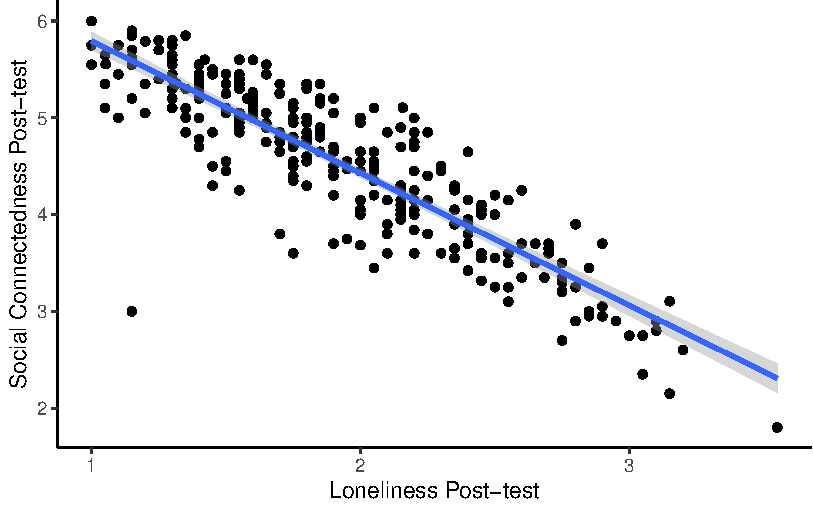
\includegraphics[width=1\textwidth,height=\textheight]{18-analysis-journey-2_files/figure-pdf/unnamed-chunk-14-1.pdf}
\end{center}

\end{tcolorbox}

\begin{enumerate}
\def\labelenumi{\arabic{enumi}.}
\setcounter{enumi}{6}
\tightlist
\item
  As we start to think about inferential statistics, we can plot the
  difference between pre- and post-test for each group. For this
  question, try and recreate the boxplot to visualise stress. Hint:
  think about if you need to restructure the data, and how you can
  present the conditions in the appropriate order.
\end{enumerate}

\begin{center}
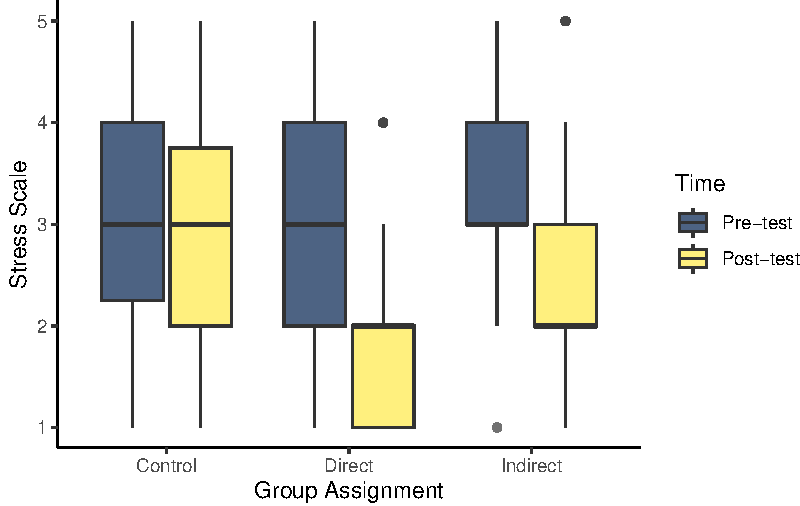
\includegraphics[width=1\textwidth,height=\textheight]{18-analysis-journey-2_files/figure-pdf/unnamed-chunk-15-1.pdf}
\end{center}

\begin{tcolorbox}[enhanced jigsaw, breakable, colframe=quarto-callout-caution-color-frame, arc=.35mm, opacitybacktitle=0.6, titlerule=0mm, colbacktitle=quarto-callout-caution-color!10!white, colback=white, toprule=.15mm, bottomtitle=1mm, toptitle=1mm, title=\textcolor{quarto-callout-caution-color}{\faFire}\hspace{0.5em}{Show me the solution}, bottomrule=.15mm, rightrule=.15mm, leftrule=.75mm, coltitle=black, left=2mm, opacityback=0]

There are two key steps before you can plot the data. First, you need to
restructure the data to long form to get one variable for pre- and
post-test. Second, post comes before pre due to alphabetical order, so
you need to create a factor to specify the order here.

\begin{Shaded}
\begin{Highlighting}[]
\NormalTok{evans\_wide }\SpecialCharTok{\%\textgreater{}\%} 
  \FunctionTok{pivot\_longer}\NormalTok{(}\AttributeTok{cols =}\NormalTok{ stress\_pre}\SpecialCharTok{:}\NormalTok{stress\_post, }
               \AttributeTok{names\_to =} \StringTok{"Stress"}\NormalTok{, }
               \AttributeTok{values\_to =} \StringTok{"Value"}\NormalTok{) }\SpecialCharTok{\%\textgreater{}\%} 
  \FunctionTok{mutate}\NormalTok{(}\AttributeTok{Stress =} \FunctionTok{factor}\NormalTok{(Stress,}
                         \AttributeTok{levels =} \FunctionTok{c}\NormalTok{(}\StringTok{"stress\_pre"}\NormalTok{, }\StringTok{"stress\_post"}\NormalTok{), }
                         \AttributeTok{labels =} \FunctionTok{c}\NormalTok{(}\StringTok{"Pre{-}test"}\NormalTok{, }\StringTok{"Post{-}test"}\NormalTok{))) }\SpecialCharTok{\%\textgreater{}\%} 
  \FunctionTok{ggplot}\NormalTok{(}\FunctionTok{aes}\NormalTok{(}\AttributeTok{x =}\NormalTok{ GroupAssignment, }\AttributeTok{y =}\NormalTok{ Value, }\AttributeTok{fill =}\NormalTok{ Stress)) }\SpecialCharTok{+} 
  \FunctionTok{geom\_boxplot}\NormalTok{(}\AttributeTok{alpha =} \FloatTok{0.7}\NormalTok{) }\SpecialCharTok{+} 
  \FunctionTok{labs}\NormalTok{(}\AttributeTok{x =} \StringTok{"Group Assignment"}\NormalTok{, }\AttributeTok{y =} \StringTok{"Stress Scale"}\NormalTok{) }\SpecialCharTok{+} 
  \FunctionTok{scale\_fill\_viridis\_d}\NormalTok{(}\AttributeTok{option =} \StringTok{"E"}\NormalTok{, }
                       \AttributeTok{name =} \StringTok{"Time"}\NormalTok{) }\SpecialCharTok{+} 
  \FunctionTok{theme\_classic}\NormalTok{()}
\end{Highlighting}
\end{Shaded}

\end{tcolorbox}

\begin{enumerate}
\def\labelenumi{\arabic{enumi}.}
\setcounter{enumi}{7}
\tightlist
\item
  Try and recreate the violin-boxplot to visualise loneliness. Hint:
  remember how to align the different elements from Chapter 7.
\end{enumerate}

\begin{center}
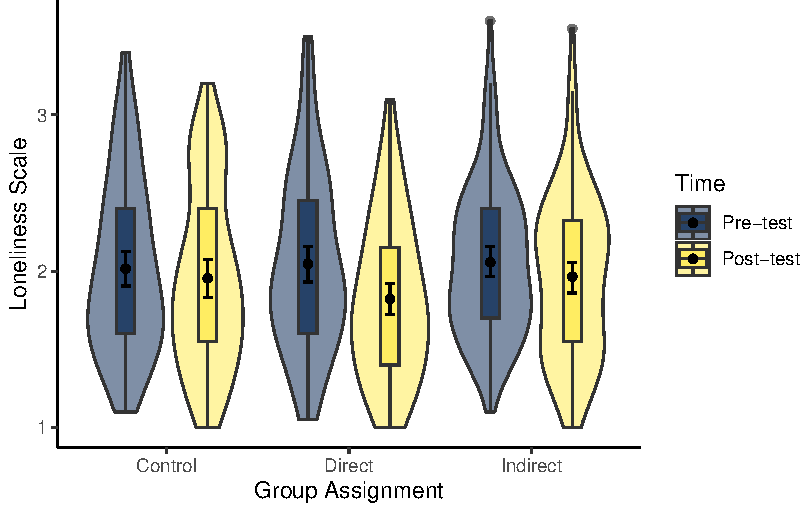
\includegraphics[width=1\textwidth,height=\textheight]{18-analysis-journey-2_files/figure-pdf/unnamed-chunk-17-1.pdf}
\end{center}

\begin{tcolorbox}[enhanced jigsaw, breakable, colframe=quarto-callout-caution-color-frame, arc=.35mm, opacitybacktitle=0.6, titlerule=0mm, colbacktitle=quarto-callout-caution-color!10!white, colback=white, toprule=.15mm, bottomtitle=1mm, toptitle=1mm, title=\textcolor{quarto-callout-caution-color}{\faFire}\hspace{0.5em}{Show me the solution}, bottomrule=.15mm, rightrule=.15mm, leftrule=.75mm, coltitle=black, left=2mm, opacityback=0]

The same hints apply as question 7 as you need to restructure the data
and create a new factor order so pre comes before post. As we have two
grouping variables, we must specify a constant position dodge value so
it does not plot weird.

\begin{Shaded}
\begin{Highlighting}[]
\CommentTok{\# specify as an object, so we only change it in one place}
\NormalTok{dodge\_value }\OtherTok{\textless{}{-}} \FloatTok{0.9}

\NormalTok{evans\_wide }\SpecialCharTok{\%\textgreater{}\%} 
  \FunctionTok{pivot\_longer}\NormalTok{(}\AttributeTok{cols =}\NormalTok{ lonely\_pre}\SpecialCharTok{:}\NormalTok{lonely\_post, }
               \AttributeTok{names\_to =} \StringTok{"Lonely"}\NormalTok{, }
               \AttributeTok{values\_to =} \StringTok{"Value"}\NormalTok{) }\SpecialCharTok{\%\textgreater{}\%} 
   \FunctionTok{mutate}\NormalTok{(}\AttributeTok{Lonely =} \FunctionTok{factor}\NormalTok{(Lonely,}
                          \AttributeTok{levels =} \FunctionTok{c}\NormalTok{(}\StringTok{"lonely\_pre"}\NormalTok{, }\StringTok{"lonely\_post"}\NormalTok{), }
                          \AttributeTok{labels =} \FunctionTok{c}\NormalTok{(}\StringTok{"Pre{-}test"}\NormalTok{, }\StringTok{"Post{-}test"}\NormalTok{))) }\SpecialCharTok{\%\textgreater{}\%} 
  \FunctionTok{ggplot}\NormalTok{(}\FunctionTok{aes}\NormalTok{(}\AttributeTok{x =}\NormalTok{ GroupAssignment, }\AttributeTok{y =}\NormalTok{ Value, }\AttributeTok{fill =}\NormalTok{ Lonely)) }\SpecialCharTok{+} 
  \FunctionTok{geom\_violin}\NormalTok{(}\AttributeTok{alpha =} \FloatTok{0.5}\NormalTok{) }\SpecialCharTok{+} 
  \FunctionTok{geom\_boxplot}\NormalTok{(}\AttributeTok{width =} \FloatTok{0.2}\NormalTok{, }
               \AttributeTok{alpha =} \FloatTok{0.7}\NormalTok{,}
               \AttributeTok{fatten =} \ConstantTok{NULL}\NormalTok{,}
               \AttributeTok{position =} \FunctionTok{position\_dodge}\NormalTok{(dodge\_value)) }\SpecialCharTok{+} 
  \FunctionTok{stat\_summary}\NormalTok{(}\AttributeTok{fun =} \StringTok{"mean"}\NormalTok{, }
               \AttributeTok{geom =} \StringTok{"point"}\NormalTok{,}
               \AttributeTok{position =} \FunctionTok{position\_dodge}\NormalTok{(dodge\_value)) }\SpecialCharTok{+}
  \FunctionTok{stat\_summary}\NormalTok{(}\AttributeTok{fun.data =} \StringTok{"mean\_cl\_boot"}\NormalTok{, }
               \AttributeTok{geom =} \StringTok{"errorbar"}\NormalTok{, }
               \AttributeTok{width =}\NormalTok{ .}\DecValTok{1}\NormalTok{,}
               \AttributeTok{position =} \FunctionTok{position\_dodge}\NormalTok{(dodge\_value)) }\SpecialCharTok{+}
  \FunctionTok{scale\_fill\_viridis\_d}\NormalTok{(}\AttributeTok{option =} \StringTok{"E"}\NormalTok{, }
                       \AttributeTok{name =} \StringTok{"Time"}\NormalTok{) }\SpecialCharTok{+} 
  \FunctionTok{labs}\NormalTok{(}\AttributeTok{x =} \StringTok{"Group Assignment"}\NormalTok{, }\AttributeTok{y =} \StringTok{"Loneliness Scale"}\NormalTok{) }\SpecialCharTok{+} 
  \FunctionTok{theme\_classic}\NormalTok{()}
\end{Highlighting}
\end{Shaded}

\end{tcolorbox}

\section{Analysing}\label{analysing}

Finally, we turn to analysis for inferential statistics. In Evans et al.
(2023), they organise the analyses from Binfet et al. (2022) into three
hypotheses. You have not covered all the skills in Research Methods 1 to
reproduce their analyses exactly, so we will work around an adapted set
based on what we currently expect of you.

We present each analysis as an overview so you can think about what
techniques from Chapters 8 and 9 would address it, give you instructions
on what analysis we have in mind if you need guidance, then present the
solution. We focus on one outcome per hypothesis, but once you are
confident you are applying and interpreting the appropriate techniques,
why not try the other outcomes yourself?

\subsection{Hypothesis 1}\label{hypothesis-1}

\begin{enumerate}
\def\labelenumi{\arabic{enumi}.}
\setcounter{enumi}{8}
\tightlist
\item
  Hypothesis 1 is that each treatment group will increase measures of
  well-being (social connectedness) and decrease measures of ill-being
  (stress and loneliness). For this question, we focus on stress, so we
  expected stress to decrease.
\end{enumerate}

\begin{tcolorbox}[enhanced jigsaw, breakable, colframe=quarto-callout-tip-color-frame, arc=.35mm, opacitybacktitle=0.6, titlerule=0mm, colbacktitle=quarto-callout-tip-color!10!white, colback=white, toprule=.15mm, bottomtitle=1mm, toptitle=1mm, title=\textcolor{quarto-callout-tip-color}{\faLightbulb}\hspace{0.5em}{Try this}, bottomrule=.15mm, rightrule=.15mm, leftrule=.75mm, coltitle=black, left=2mm, opacityback=0]

There are two ways you could approach this. Either as the whole sample,
or like Evans et al. (2023) present to focus on each group separately.
Think about what techniques from Chapters 8 and 9 would let you test the
hypothesis that each treatment group will decrease stress at post-test
compared to pre-test.

\end{tcolorbox}

\begin{tcolorbox}[enhanced jigsaw, breakable, colframe=quarto-callout-note-color-frame, arc=.35mm, opacitybacktitle=0.6, titlerule=0mm, colbacktitle=quarto-callout-note-color!10!white, colback=white, toprule=.15mm, bottomtitle=1mm, toptitle=1mm, title=\textcolor{quarto-callout-note-color}{\faInfo}\hspace{0.5em}{Show me the task list}, bottomrule=.15mm, rightrule=.15mm, leftrule=.75mm, coltitle=black, left=2mm, opacityback=0]

For the solution below, we are focusing on the whole sample to test
whether everyone decreased stress in post-test, but you could approach
it by separating the data into the three groups and then testing for the
difference per group.

To test whether an outcome decreases between conditions in the same
participants, we need a model suitable for a within-subjects design. In
Chapter 9, we covered in \hyperref[09-bonus]{the bonus section} how to
test the difference in conditions either through a paired samples-test
or linear model with fixed intercept on the difference score.

\begin{enumerate}
\def\labelenumi{\arabic{enumi}.}
\item
  Calculate the difference between stress pre- and post-test.
\item
  Fit a linear model on the difference score with a fixed intercept and
  no predictor.
\item
  Look at the intercept, is it positive or negative? If you calculated
  pre-test minus post-test, you would be looking for a postive
  difference as we expect lower stress at post-test. For hypothesis
  testing, is the \emph{p}-value lower than alpha?
\item
  What is the effect size? How much did stress change from pre-test to
  post-test? What is the confidence interval around the effect size?
\end{enumerate}

\end{tcolorbox}

\begin{tcolorbox}[enhanced jigsaw, breakable, colframe=quarto-callout-caution-color-frame, arc=.35mm, opacitybacktitle=0.6, titlerule=0mm, colbacktitle=quarto-callout-caution-color!10!white, colback=white, toprule=.15mm, bottomtitle=1mm, toptitle=1mm, title=\textcolor{quarto-callout-caution-color}{\faFire}\hspace{0.5em}{Show me the solution}, bottomrule=.15mm, rightrule=.15mm, leftrule=.75mm, coltitle=black, left=2mm, opacityback=0]

In the code below, we first calculate a difference score by substracting
stress post-test from stress pre-test.

We then fit a linear model on this difference score and add a fixed
intercept as we have no predictor.

Consistent with hypothesis 1, stress was lower at post-test compared to
pre-test across all participants. On average, participants decreased
their stress score by 0.83 points (\(b_0\) = 0.83, 95\% CI = {[}0.72,
0.95{]}, \emph{p} \textless{} .001).

\begin{Shaded}
\begin{Highlighting}[]
\NormalTok{evans\_wide }\OtherTok{\textless{}{-}}\NormalTok{ evans\_wide }\SpecialCharTok{\%\textgreater{}\%} 
  \FunctionTok{mutate}\NormalTok{(}\AttributeTok{stress\_diff =}\NormalTok{ stress\_pre }\SpecialCharTok{{-}}\NormalTok{ stress\_post)}

\NormalTok{lm\_stress }\OtherTok{\textless{}{-}} \FunctionTok{lm}\NormalTok{(stress\_diff }\SpecialCharTok{\textasciitilde{}} \DecValTok{1}\NormalTok{, }
                \AttributeTok{data =}\NormalTok{ evans\_wide)}

\FunctionTok{summary}\NormalTok{(lm\_stress)}

\FunctionTok{confint}\NormalTok{(lm\_stress)}
\end{Highlighting}
\end{Shaded}

\begin{verbatim}

Call:
lm(formula = stress_diff ~ 1, data = evans_wide)

Residuals:
    Min      1Q  Median      3Q     Max 
-2.8345 -0.8345  0.1655  0.1655  3.1655 

Coefficients:
            Estimate Std. Error t value Pr(>|t|)    
(Intercept)  0.83451    0.05657   14.75   <2e-16 ***
---
Signif. codes:  0 '***' 0.001 '**' 0.01 '*' 0.05 '.' 0.1 ' ' 1

Residual standard error: 0.9534 on 283 degrees of freedom

                2.5 %    97.5 %
(Intercept) 0.7231517 0.9458623
\end{verbatim}

\end{tcolorbox}

\subsection{Hypothesis 2}\label{hypothesis-2}

\begin{enumerate}
\def\labelenumi{\arabic{enumi}.}
\setcounter{enumi}{9}
\tightlist
\item
  In Hypothesis 2, we predict that the direct and indirect contact
  groups will have higher well-being and lower ill-being measures
  compared to the control group. For this question, we focus on social
  connectedness at post-test for a measure of well-being, so we expect
  higher scores in the direct and indirect groups.
\end{enumerate}

\begin{tcolorbox}[enhanced jigsaw, breakable, colframe=quarto-callout-tip-color-frame, arc=.35mm, opacitybacktitle=0.6, titlerule=0mm, colbacktitle=quarto-callout-tip-color!10!white, colback=white, toprule=.15mm, bottomtitle=1mm, toptitle=1mm, title=\textcolor{quarto-callout-tip-color}{\faLightbulb}\hspace{0.5em}{Try this}, bottomrule=.15mm, rightrule=.15mm, leftrule=.75mm, coltitle=black, left=2mm, opacityback=0]

Think about what techniques from Chapters 8 and 9 would let you test the
hypothesis that the direct and indirect groups both increase social
connectedness at post-test compared to the control group. Think of how
you could focus on two groups at a time per analysis.

\end{tcolorbox}

\begin{tcolorbox}[enhanced jigsaw, breakable, colframe=quarto-callout-note-color-frame, arc=.35mm, opacitybacktitle=0.6, titlerule=0mm, colbacktitle=quarto-callout-note-color!10!white, colback=white, toprule=.15mm, bottomtitle=1mm, toptitle=1mm, title=\textcolor{quarto-callout-note-color}{\faInfo}\hspace{0.5em}{Show me the task list}, bottomrule=.15mm, rightrule=.15mm, leftrule=.75mm, coltitle=black, left=2mm, opacityback=0]

For the solution below, we apply two tests. We focus on the direct and
control groups by filtering out indirect, then we focus on indirect and
control by filtering out direct.

To test the difference between two groups on one outcome, we need a
model suitable for a between-subjects design. In Chapter 9, we covered
\hyperref[09-categorical]{linear regression with one categorical
predictor} how to test the difference in an outcome between two groups.

\begin{enumerate}
\def\labelenumi{\arabic{enumi}.}
\item
  Fit a linear model on the outcome social connectedness post-test with
  a categorical predictor of group. You will need to fit two models, one
  where you filter out the indirect group and one where you filter out
  the direct group.
\item
  Look at the intercept, what is the predicted value for the reference
  group? Look at the slope, what is the estimated change to the target
  group? For hypothesis 2, is the direct/indirect group higher on social
  connectedness compared to control? For hypothesis testing, is the
  \emph{p}-value lower than alpha?
\item
  What is the effect size? How much did the two groups differ on social
  connectedness? What is the confidence interval around the effect size?
\end{enumerate}

\end{tcolorbox}

\begin{tcolorbox}[enhanced jigsaw, breakable, colframe=quarto-callout-caution-color-frame, arc=.35mm, opacitybacktitle=0.6, titlerule=0mm, colbacktitle=quarto-callout-caution-color!10!white, colback=white, toprule=.15mm, bottomtitle=1mm, toptitle=1mm, title=\textcolor{quarto-callout-caution-color}{\faFire}\hspace{0.5em}{Show me the solution}, bottomrule=.15mm, rightrule=.15mm, leftrule=.75mm, coltitle=black, left=2mm, opacityback=0]

In the code below, we first fit a linear model on social connectedness
post-test and focus on the direct and control groups. There are
different ways you could ignore the indirect group, but here we filter
the data as we pass the data to the \texttt{lm()} function.

The direct group increased social connectedness post-test on average
0.15 points compared to the control group, but the difference was not
statistically significant (\(b_1\) = 0.15, 95\% CI = {[}-0.09, 0.39{]},
\emph{p} = .207).

\begin{Shaded}
\begin{Highlighting}[]
\NormalTok{lm\_direct }\OtherTok{\textless{}{-}} \FunctionTok{lm}\NormalTok{(social\_post }\SpecialCharTok{\textasciitilde{}}\NormalTok{ GroupAssignment, }
                 \AttributeTok{data =} \FunctionTok{filter}\NormalTok{(evans\_wide,}
\NormalTok{                               GroupAssignment }\SpecialCharTok{!=} \StringTok{"Indirect"}\NormalTok{))}

\FunctionTok{summary}\NormalTok{(lm\_direct)}

\FunctionTok{confint}\NormalTok{(lm\_direct)}
\end{Highlighting}
\end{Shaded}

\begin{verbatim}

Call:
lm(formula = social_post ~ GroupAssignment, data = filter(evans_wide, 
    GroupAssignment != "Indirect"))

Residuals:
    Min      1Q  Median      3Q     Max 
-2.2940 -0.5905  0.1338  0.6560  1.3560 

Coefficients:
                      Estimate Std. Error t value Pr(>|t|)    
(Intercept)            4.49054    0.08596  52.239   <2e-16 ***
GroupAssignmentDirect  0.15349    0.12125   1.266    0.207    
---
Signif. codes:  0 '***' 0.001 '**' 0.01 '*' 0.05 '.' 0.1 ' ' 1

Residual standard error: 0.8334 on 187 degrees of freedom
Multiple R-squared:  0.008497,  Adjusted R-squared:  0.003195 
F-statistic: 1.603 on 1 and 187 DF,  p-value: 0.2071

                            2.5 %    97.5 %
(Intercept)            4.32096331 4.6601179
GroupAssignmentDirect -0.08569829 0.3926749
\end{verbatim}

The indirect group increased social connectedness post-test compared to
the control group, but the difference was very small and not
statistically significant (\(b_1\) = 0.01, 95\% CI = {[}-0.23, 0.25{]},
\emph{p} = .936).

\begin{Shaded}
\begin{Highlighting}[]
\NormalTok{lm\_indirect }\OtherTok{\textless{}{-}} \FunctionTok{lm}\NormalTok{(social\_post }\SpecialCharTok{\textasciitilde{}}\NormalTok{ GroupAssignment, }
                 \AttributeTok{data =} \FunctionTok{filter}\NormalTok{(evans\_wide,}
\NormalTok{                               GroupAssignment }\SpecialCharTok{!=} \StringTok{"Direct"}\NormalTok{))}

\FunctionTok{summary}\NormalTok{(lm\_indirect)}

\FunctionTok{confint}\NormalTok{(lm\_indirect)}
\end{Highlighting}
\end{Shaded}

\begin{verbatim}

Call:
lm(formula = social_post ~ GroupAssignment, data = filter(evans_wide, 
    GroupAssignment != "Direct"))

Residuals:
     Min       1Q   Median       3Q      Max 
-2.70037 -0.59054  0.05946  0.64963  1.34963 

Coefficients:
                        Estimate Std. Error t value Pr(>|t|)    
(Intercept)             4.490541   0.087155   51.52   <2e-16 ***
GroupAssignmentIndirect 0.009833   0.122931    0.08    0.936    
---
Signif. codes:  0 '***' 0.001 '**' 0.01 '*' 0.05 '.' 0.1 ' ' 1

Residual standard error: 0.845 on 187 degrees of freedom
Multiple R-squared:  3.422e-05, Adjusted R-squared:  -0.005313 
F-statistic: 0.006398 on 1 and 187 DF,  p-value: 0.9363

                             2.5 %    97.5 %
(Intercept)              4.3186067 4.6624745
GroupAssignmentIndirect -0.2326772 0.2523439
\end{verbatim}

In Evans et al. (2023), the direct vs control comparison is significant,
but they approached the analysis differently using a technique you will
not learn until Research Methods 2. They control for pre-test scores by
using it as an additional predictor, but you have not learnt about
multiple regression yet.

\end{tcolorbox}

\subsection{Hypothesis 3}\label{hypothesis-3}

\begin{enumerate}
\def\labelenumi{\arabic{enumi}.}
\setcounter{enumi}{10}
\tightlist
\item
  Finally, the third hypothesis focuses on the difference between the
  two contact groups. They predict that the direct contact group will
  lead to higher well-being and lower ill-being compared to the indirect
  contact group. For this question, we focus on loneliness post-test for
  a measure of ill-being, so we expect lower scores in the direct group.
\end{enumerate}

\begin{tcolorbox}[enhanced jigsaw, breakable, colframe=quarto-callout-tip-color-frame, arc=.35mm, opacitybacktitle=0.6, titlerule=0mm, colbacktitle=quarto-callout-tip-color!10!white, colback=white, toprule=.15mm, bottomtitle=1mm, toptitle=1mm, title=\textcolor{quarto-callout-tip-color}{\faLightbulb}\hspace{0.5em}{Try this}, bottomrule=.15mm, rightrule=.15mm, leftrule=.75mm, coltitle=black, left=2mm, opacityback=0]

Think about what techniques from Chapters 8 and 9 would let you test the
hypothesis that the direct group decreases loneliness at post-test
compared to the indirect group.

\end{tcolorbox}

\begin{tcolorbox}[enhanced jigsaw, breakable, colframe=quarto-callout-note-color-frame, arc=.35mm, opacitybacktitle=0.6, titlerule=0mm, colbacktitle=quarto-callout-note-color!10!white, colback=white, toprule=.15mm, bottomtitle=1mm, toptitle=1mm, title=\textcolor{quarto-callout-note-color}{\faInfo}\hspace{0.5em}{Show me the task list}, bottomrule=.15mm, rightrule=.15mm, leftrule=.75mm, coltitle=black, left=2mm, opacityback=0]

For this analysis, we focus on the final combination of groups, this
time ignoring the control group.

To test the difference between two groups on one outcome, we need a
model suitable for a between-subjects design. In Chapter 9, we covered
\hyperref[09-categorical]{linear regression with one categorical
predictor} how to test the difference in an outcome between two groups.

\begin{enumerate}
\def\labelenumi{\arabic{enumi}.}
\item
  Fit a linear model on the outcome loneliness post-test with a
  categorical predictor of group. Filter the data to just focus on the
  direct and indirect contact groups.
\item
  Look at the intercept, what is the predicted value for the reference
  group? Look at the slope, what is the estimated change to the target
  group? For hypothesis 3, is the direct group lower on loneliness
  compared to indirect? For hypothesis testing, is the \emph{p}-value
  lower than alpha?
\item
  What is the effect size? How much did the two groups differ on
  loneliness? What is the confidence interval around the effect size?
\end{enumerate}

\end{tcolorbox}

\begin{tcolorbox}[enhanced jigsaw, breakable, colframe=quarto-callout-caution-color-frame, arc=.35mm, opacitybacktitle=0.6, titlerule=0mm, colbacktitle=quarto-callout-caution-color!10!white, colback=white, toprule=.15mm, bottomtitle=1mm, toptitle=1mm, title=\textcolor{quarto-callout-caution-color}{\faFire}\hspace{0.5em}{Show me the solution}, bottomrule=.15mm, rightrule=.15mm, leftrule=.75mm, coltitle=black, left=2mm, opacityback=0]

In the code below, we first fit a linear model on loneliness post-test
and focus on the direct and indirect groups. There are different ways
you could ignore the indirect group, but here we filter the data as we
pass the data to the \texttt{lm()} function.

The direct group decreased loneliness post-test on average 0.14 points
compared to the indirect group, but the difference was not statistically
significant (\(b_1\) = 0.14, 95\% CI = {[}-0.01, 0.29{]}, \emph{p} =
.060).

\begin{Shaded}
\begin{Highlighting}[]
\NormalTok{lm\_contact }\OtherTok{\textless{}{-}} \FunctionTok{lm}\NormalTok{(lonely\_post }\SpecialCharTok{\textasciitilde{}}\NormalTok{ GroupAssignment, }
                 \AttributeTok{data =} \FunctionTok{filter}\NormalTok{(evans\_wide,}
\NormalTok{                               GroupAssignment }\SpecialCharTok{!=} \StringTok{"Control"}\NormalTok{))}

\FunctionTok{summary}\NormalTok{(lm\_contact)}

\FunctionTok{confint}\NormalTok{(lm\_contact)}
\end{Highlighting}
\end{Shaded}

\begin{verbatim}

Call:
lm(formula = lonely_post ~ GroupAssignment, data = filter(evans_wide, 
    GroupAssignment != "Control"))

Residuals:
     Min       1Q   Median       3Q      Max 
-0.96457 -0.42130 -0.06457  0.32645  1.58543 

Coefficients:
                        Estimate Std. Error t value Pr(>|t|)    
(Intercept)              1.82355    0.05267  34.625   <2e-16 ***
GroupAssignmentIndirect  0.14102    0.07448   1.893   0.0598 .  
---
Signif. codes:  0 '***' 0.001 '**' 0.01 '*' 0.05 '.' 0.1 ' ' 1

Residual standard error: 0.5133 on 188 degrees of freedom
Multiple R-squared:  0.01871,   Adjusted R-squared:  0.01349 
F-statistic: 3.585 on 1 and 188 DF,  p-value: 0.05983

                               2.5 %    97.5 %
(Intercept)              1.719655160 1.9274363
GroupAssignmentIndirect -0.005898489 0.2879484
\end{verbatim}

Like hypothesis 2, Evans et al. (2023) report the direct vs indirect
comparison as significant, but they approached the analysis differently
using a technique you will not learn until Research Methods 2. They
control for pre-test scores by using it as an additional predictor, but
you have not learnt about multiple regression yet.

\end{tcolorbox}

\section{Conclusion}\label{conclusion-1}

Well done! Hopefully you recognised how far your skills have come to be
able to do this independently, regardless of how many hints you needed.
We are really starting to pile the skills up you have learnt so far,
from simply using R Markdown files, to wrangling data, to visualising
data, to finally applying modelling techniques for your inferential
statistics.

If you are curious, you can read Evans et al. (2023) to see how they
walk through wrangling and analysing the data. Some of the techniques we
do not cover in Research Methods 1, but they have some great features
like highlighting common student mistakes.

\bookmarksetup{startatroot}

\chapter*{References}\label{references}
\addcontentsline{toc}{chapter}{References}

\markboth{References}{References}

\phantomsection\label{refs}
\begin{CSLReferences}{1}{0}
\bibitem[\citeproctext]{ref-alter_vssl_2024}
Alter, U., Dang, C., Kunicki, Z. J., \& Counsell, A. (2024). The {VSSL}
scale: {A} brief instructor tool for assessing students' perceived value
of software to learning statistics. \emph{Teaching Statistics},
\emph{46}(3). \url{https://doi.org/10.1111/test.12374}

\bibitem[\citeproctext]{ref-bakker_recommendations_2020}
Bakker, M., Veldkamp, C. L. S., Akker, O. R. van den, Assen, M. A. L. M.
van, Crompvoets, E., Ong, H. H., \& Wicherts, J. M. (2020).
Recommendations in pre-registrations and internal review board proposals
promote formal power analyses but do not increase sample size.
\emph{PLoS ONE}, \emph{15}(7), e0236079.
\url{https://doi.org/10.1371/journal.pone.0236079}

\bibitem[\citeproctext]{ref-bartlett_no_2022}
Bartlett, J. E., Jenks, R., \& Wilson, N. (2022). No {Meaningful}
{Difference} in {Attentional} {Bias} {Between} {Daily} and {Non}-{Daily}
{Smokers}. \emph{Journal of Trial \& Error}.
\url{https://doi.org/10.36850/e11}

\bibitem[\citeproctext]{ref-bartlett_power_2022}
Bartlett, J., \& Charles, S. (2022). Power to the {People}: {A}
{Beginner}'s {Tutorial} to {Power} {Analysis} using jamovi.
\emph{Meta-Psychology}, \emph{6}.
\url{https://doi.org/10.15626/MP.2021.3078}

\bibitem[\citeproctext]{ref-bem_feeling_2011}
Bem, D. J. (2011). Feeling the future: {Experimental} evidence for
anomalous retroactive influences on cognition and affect. \emph{Journal
of Personality and Social Psychology}, \emph{100}(3), 407--425.
\url{https://doi.org/10.1037/a0021524}

\bibitem[\citeproctext]{ref-binfet_importance_2022}
Binfet, J.-T., Green, F. L. L., \& Draper, Z. A. (2022). The
{Importance} of {Client}--{Canine} {Contact} in {Canine}-{Assisted}
{Interventions}: {A} {Randomized} {Controlled} {Trial}.
\emph{Anthrozoös}, \emph{35}(1), 1--22.
\url{https://doi.org/10.1080/08927936.2021.1944558}

\bibitem[\citeproctext]{ref-blanca_effect_2018}
Blanca, M. J., Alarcón, R., Arnau, J., Bono, R., \& Bendayan, R. (2018).
Effect of variance ratio on {ANOVA} robustness: {Might} 1.5 be the
limit? \emph{Behavior Research Methods}, \emph{50}(3), 937--962.
\url{https://doi.org/10.3758/s13428-017-0918-2}

\bibitem[\citeproctext]{ref-Champely2020_pwr}
Champely, S. (2020). \emph{Pwr: Basic functions for power analysis}.
\url{https://CRAN.R-project.org/package=pwr}

\bibitem[\citeproctext]{ref-dasu2003}
Dasu, T., \& Johnson, T. (2003). \emph{Exploratory data mining and data
cleaning}. Wiley-Interscience.

\bibitem[\citeproctext]{ref-dawtry_why_2015}
Dawtry, R. J., Sutton, R. M., \& Sibley, C. G. (2015). Why {Wealthier}
{People} {Think} {People} {Are} {Wealthier}, and {Why} {It} {Matters}:
{From} {Social} {Sampling} to {Attitudes} to {Redistribution}.
\emph{Psychological Science}, \emph{26}(9), 1389--1400.
\url{https://doi.org/10.1177/0956797615586560}

\bibitem[\citeproctext]{ref-evans_repurposing_2023}
Evans, C., Cipolli, W., Draper, Z. A., \& Binfet, J.-T. (2023).
Repurposing a {Peer}-{Reviewed} {Publication} to {Engage} {Students} in
{Statistics}: {An} {Illustration} of {Study} {Design}, {Data}
{Collection}, and {Analysis}. \emph{Journal of Statistics and Data
Science Education}, \emph{0}(0), 1--21.
\url{https://doi.org/10.1080/26939169.2023.2238018}

\bibitem[\citeproctext]{ref-harms_making_2018}
Harms, C., \& Lakens, D. (2018). Making 'null effects' informative:
Statistical techniques and inferential frameworks. \emph{Journal of
Clinical and Translational Research}, \emph{3}(Suppl 2), 382--393.
\url{https://www.ncbi.nlm.nih.gov/pmc/articles/PMC6412612/}

\bibitem[\citeproctext]{ref-hoffman_students_2021}
Hoffman, H. J., \& Elmi, A. F. (2021). Do {Students} {Learn} {More} from
{Erroneous} {Code}? {Exploring} {Student} {Performance} and
{Satisfaction} in an {Error}-{Free} {Versus} an {Error}-full {SAS}®
{Programming} {Environment}. \emph{Journal of Statistics and Data
Science Education}, \emph{0}(0), 1--13.
\url{https://doi.org/10.1080/26939169.2021.1967229}

\bibitem[\citeproctext]{ref-irving_correcting_2022}
Irving, D., Clark, R. W. A., Lewandowsky, S., \& Allen, P. J. (2022).
Correcting statistical misinformation about scientific findings in the
media: {Causation} versus correlation. \emph{Journal of Experimental
Psychology. Applied}. \url{https://doi.org/10.1037/xap0000408}

\bibitem[\citeproctext]{ref-jakobsen_when_2017}
Jakobsen, J. C., Gluud, C., Wetterslev, J., \& Winkel, P. (2017). When
and how should multiple imputation be used for handling missing data in
randomised clinical trials -- a practical guide with flowcharts.
\emph{BMC Medical Research Methodology}, \emph{17}(1), 162.
\url{https://doi.org/10.1186/s12874-017-0442-1}

\bibitem[\citeproctext]{ref-james_computer_2015}
James, E. L., Bonsall, M. B., Hoppitt, L., Tunbridge, E. M., Geddes, J.
R., Milton, A. L., \& Holmes, E. A. (2015). Computer {Game} {Play}
{Reduces} {Intrusive} {Memories} of {Experimental} {Trauma} via
{Reconsolidation}-{Update} {Mechanisms}: \emph{Psychological Science},
\emph{26}(8), 1201--1215. \url{https://doi.org/10.1177/0956797615583071}

\bibitem[\citeproctext]{ref-knief_violating_2021}
Knief, U., \& Forstmeier, W. (2021). Violating the normality assumption
may be the lesser of two evils. \emph{Behavior Research Methods},
\emph{53}(6), 2576--2590.
\url{https://doi.org/10.3758/s13428-021-01587-5}

\bibitem[\citeproctext]{ref-lakens_sample_2022}
Lakens, D. (2022). Sample {Size} {Justification}. \emph{Collabra:
Psychology}, \emph{8}(1), 33267.
\url{https://doi.org/10.1525/collabra.33267}

\bibitem[\citeproctext]{ref-lakens_improving_2020}
Lakens, D., McLatchie, N., Isager, P. M., Scheel, A. M., \& Dienes, Z.
(2020). Improving {Inferences} {About} {Null} {Effects} {With} {Bayes}
{Factors} and {Equivalence} {Tests}. \emph{The Journals of Gerontology:
Series B}, \emph{75}(1), 45--57.
\url{https://doi.org/10.1093/geronb/gby065}

\bibitem[\citeproctext]{ref-lakens_equivalence_2018}
Lakens, D., Scheel, A. M., \& Isager, P. M. (2018). Equivalence
{Testing} for {Psychological} {Research}: {A} {Tutorial}. \emph{Advances
in Methods and Practices in Psychological Science}, \emph{1}(2),
259--269. \url{https://doi.org/10.1177/2515245918770963}

\bibitem[\citeproctext]{ref-leys_how_2019}
Leys, C., Delacre, M., Mora, Y. L., Lakens, D., \& Ley, C. (2019). How
to {Classify}, {Detect}, and {Manage} {Univariate} and {Multivariate}
{Outliers}, {With} {Emphasis} on {Pre}-{Registration}.
\emph{International Review of Social Psychology}, \emph{32}(1), 5.
\url{https://doi.org/10.5334/irsp.289}

\bibitem[\citeproctext]{ref-lopez_visual_2023}
Lopez, A., Choi, A. K., Dellawar, N. C., Cullen, B. C., Avila Contreras,
S., Rosenfeld, D. L., \& Tomiyama, A. J. (2023). Visual cues and food
intake: {A} preregistered replication of {Wansink} et al (2005).
\emph{Journal of Experimental Psychology: General}.
\url{https://doi.org/10.1037/xge0001503.supp}

\bibitem[\citeproctext]{ref-nordmann_data_2022}
Nordmann, E., McAleer, P., Toivo, W., Paterson, H., \& DeBruine, L. M.
(2022). Data {Visualization} {Using} {R} for {Researchers} {Who} {Do}
{Not} {Use} {R}. \emph{Advances in Methods and Practices in
Psychological Science}, \emph{5}(2), 25152459221074654.
\url{https://doi.org/10.1177/25152459221074654}

\bibitem[\citeproctext]{ref-orben_crud_2020}
Orben, A., \& Lakens, D. (2020). Crud ({Re}){Defined}. \emph{Advances in
Methods and Practices in Psychological Science}, \emph{3}(2), 238--247.
\url{https://doi.org/10.1177/2515245920917961}

\bibitem[\citeproctext]{ref-przybylski_large-scale_2017}
Przybylski, A. K., \& Weinstein, N. (2017). A {Large}-{Scale} {Test} of
the {Goldilocks} {Hypothesis}: {Quantifying} the {Relations} {Between}
{Digital}-{Screen} {Use} and the {Mental} {Well}-{Being} of
{Adolescents}. \emph{Psychological Science}, \emph{28}(2), 204--215.
\url{https://doi.org/10.1177/0956797616678438}

\bibitem[\citeproctext]{ref-RCoreTeam_2024}
R Core Team. (2024). \emph{R: A language and environment for statistical
computing}. R Foundation for Statistical Computing.
\url{https://www.R-project.org/}

\bibitem[\citeproctext]{ref-weissgerber_reveal_2019}
Weissgerber, T. L., Winham, S. J., Heinzen, E. P., Milin-Lazovic, J. S.,
Garcia-Valencia, O., Bukumiric, Z., Savic, M. D., Garovic, V. D., \&
Milic, N. M. (2019). Reveal, {Don}'t {Conceal}. \emph{Circulation},
\emph{140}(18), 1506--1518.
\url{https://doi.org/10.1161/CIRCULATIONAHA.118.037777}

\bibitem[\citeproctext]{ref-wickham_tidy_2014}
Wickham, H. (2014). Tidy {Data}. \emph{Journal of Statistical Software},
\emph{59}, 1--23. \url{https://doi.org/10.18637/jss.v059.i10}

\bibitem[\citeproctext]{ref-tidyverse}
Wickham, H. (2017). \emph{Tidyverse: Easily install and load the
'tidyverse'}. \url{https://CRAN.R-project.org/package=tidyverse}

\bibitem[\citeproctext]{ref-wingen_no_2020}
Wingen, T., Berkessel, J. B., \& Englich, B. (2020). No {Replication},
{No} {Trust}? {How} {Low} {Replicability} {Influences} {Trust} in
{Psychology}. \emph{Social Psychological and Personality Science},
\emph{11}(4), 454--463. \url{https://doi.org/10.1177/1948550619877412}

\bibitem[\citeproctext]{ref-witt2018}
Witt, J. K., Tenhundfeld, N. L., \& Tymoski, M. J. (2018). Is there a
chastity belt on perception? \emph{Psychological Science}, \emph{29}(1),
139--146.

\bibitem[\citeproctext]{ref-woodworth_data_2018}
Woodworth, R. J., O'Brien-Malone, A., Diamond, M. R., \& Schüz, B.
(2018). Data from, {``{Web}-based {Positive} {Psychology}
{Interventions}: {A} {Reexamination} of {Effectiveness}.''}
\emph{Journal of Open Psychology Data}, \emph{6}(1), 1.
\url{https://doi.org/10.5334/jopd.35}

\bibitem[\citeproctext]{ref-zhang_present_2014}
Zhang, T., Kim, T., Brooks, A. W., Gino, F., \& Norton, M. I. (2014). A
{``{Present}''} for the {Future}: {The} {Unexpected} {Value} of
{Rediscovery}. \emph{Psychological Science}, \emph{25}(10), 1851--1860.
\url{https://doi.org/10.1177/0956797614542274}

\end{CSLReferences}

\bookmarksetup{startatroot}

\chapter*{Using our materials}\label{using-our-materials}
\addcontentsline{toc}{chapter}{Using our materials}

\markboth{Using our materials}{Using our materials}

All PsyTeachR resources are open-access with Creative Commons licences
(see below). You are free to reuse, remix, and adapt our materials with
attribution. If you do use any of our work, please complete this
\href{https://forms.office.com/e/v8Sk0UpP6Q}{short form} so that we can
track our impact.

\section*{Licence}\label{licence}
\addcontentsline{toc}{section}{Licence}

\markright{Licence}

This book is licensed under Creative Commons Attribution-ShareAlike 4.0
International License
\href{https://creativecommons.org/licenses/by-sa/4.0/}{(CC-BY-SA 4.0)}.
You are free to share and adapt this book. You must give appropriate
credit, provide a link to the license, and indicate if changes were
made. If you adapt the material, you must distribute your contributions
under the same license as the original.

\section*{Citation}\label{citation}
\addcontentsline{toc}{section}{Citation}

\markright{Citation}

Bartlett, J.E. \& Toivo, W. (2024). Fundamentals of Quantitative
Analysis (Version 3.0).
https://github.com/PsyTeachR/quant-fundamentals-v3

\cleardoublepage
\phantomsection
\addcontentsline{toc}{part}{Appendices}
\appendix

\chapter{Additional Resources}\label{additional-resources}

\begin{figure}[H]

{\centering 
\includegraphics[width=1\textwidth,height=\textheight]{images/kitteh.png}

}

\caption{The truth about programming}

\end{figure}%

If you would like additional practice, you can check out the other UofG
PsyTeachR course books.

\begin{itemize}
\tightlist
\item
  \href{https://psyteachr.github.io/ug1-practical/}{Level 1} - Intro to
  R (overlaps with Msc Conv book), data wrangling, data viz, descriptive
  statistics\\
\item
  \href{https://psyteachr.github.io/ug2-practical/}{Level 2} - Our
  second-year undergraduate course introduces statistical concepts such
  as permutation tests,t-tests, NHST, alpha, power, effect size, and
  sample size. Semester 2 focusses on correlations and the general
  linear model.
\item
  \href{https://psyteachr.github.io/ug3-stats/}{Level 3}: This
  third-year undergraduate course teaches students how to specify,
  estimate, and interpret statistical models corresponding to various
  study designs, using a General Linear Models approach.
\item
  \href{https://psyteachr.github.io/msc-data-skills/}{MSc Data Skills}:
  This course provides an overview of skills needed for reproducible
  research and open science using the statistical programming language
  R. Students will learn about data visualisation, data tidying and
  wrangling, archiving, iteration and functions, probability and data
  simulations, general linear models, and reproducible workflows.
\end{itemize}

We also highly recommend the following, they will help practice your
data wrangling skills but also they're great options if you're enjoying
R and want to stretch yourself:

\begin{itemize}
\tightlist
\item
  \href{https://sites.trinity.edu/osl}{Open Stats Lab} - this wonderful
  resource gives you practice at running statistical tests by providing
  you with datasets from published papers.
\item
  \href{https://r4ds.had.co.nz/}{R for Data Science} - written by the
  authors of the tidyverse, this is a great resource for additional data
  wrangling practice and more depth on many of the tidyverse functions.
\item
  \href{https://www.tidytextmining.com/}{Text Mining with R} - Shows you
  how to use R to work with text. This isn't something we cover in this
  course, but it uses the same data wrangling skills and be a very
  useful additional skill to have.
\item
  \href{https://bbc.github.io/rcookbook/\#how_to_create_bbc_style_graphics}{How
  to make BBC style graphics} - Ever wondered how the BBC News makes
  their data visualisation? Well, now you can make your own!
\item
  \href{https://socviz.co/}{Data Vizualisation} - this is an entire book
  on data visualisation and goes into detail on how to take
  \texttt{ggplot} to its limits.
\end{itemize}

\chapter{Citing R and RStudio}\label{citing-r-rstudio}

How to cite R and RStudio

You may be some way off writing a scientific report where you have to
cite and reference R, however, when the time comes it is important to do
so to give the people who built it (most of them for free!) credit. You
should provide separate citations for R, RStudio, and the packages you
use.

To get the citation for the version of R you are using, simply run the
\texttt{citation()} function which will always provide you with the most
recent citation.

\begin{Shaded}
\begin{Highlighting}[]
\FunctionTok{citation}\NormalTok{()}
\end{Highlighting}
\end{Shaded}

\begin{verbatim}
To cite R in publications use:

  R Core Team (2024). _R: A Language and Environment for Statistical
  Computing_. R Foundation for Statistical Computing, Vienna, Austria.
  <https://www.R-project.org/>.

A BibTeX entry for LaTeX users is

  @Manual{,
    title = {R: A Language and Environment for Statistical Computing},
    author = {{R Core Team}},
    organization = {R Foundation for Statistical Computing},
    address = {Vienna, Austria},
    year = {2024},
    url = {https://www.R-project.org/},
  }

We have invested a lot of time and effort in creating R, please cite it
when using it for data analysis. See also 'citation("pkgname")' for
citing R packages.
\end{verbatim}

To generate the citation for any packages you are using, you can also
use the \texttt{citation()} function with the name of the package you
wish to cite.

\begin{Shaded}
\begin{Highlighting}[]
\FunctionTok{citation}\NormalTok{(}\StringTok{"tidyverse"}\NormalTok{)}
\end{Highlighting}
\end{Shaded}

\begin{verbatim}
To cite package 'tidyverse' in publications use:

  Wickham H, Averick M, Bryan J, Chang W, McGowan LD, François R,
  Grolemund G, Hayes A, Henry L, Hester J, Kuhn M, Pedersen TL, Miller
  E, Bache SM, Müller K, Ooms J, Robinson D, Seidel DP, Spinu V,
  Takahashi K, Vaughan D, Wilke C, Woo K, Yutani H (2019). "Welcome to
  the tidyverse." _Journal of Open Source Software_, *4*(43), 1686.
  doi:10.21105/joss.01686 <https://doi.org/10.21105/joss.01686>.

A BibTeX entry for LaTeX users is

  @Article{,
    title = {Welcome to the {tidyverse}},
    author = {Hadley Wickham and Mara Averick and Jennifer Bryan and Winston Chang and Lucy D'Agostino McGowan and Romain François and Garrett Grolemund and Alex Hayes and Lionel Henry and Jim Hester and Max Kuhn and Thomas Lin Pedersen and Evan Miller and Stephan Milton Bache and Kirill Müller and Jeroen Ooms and David Robinson and Dana Paige Seidel and Vitalie Spinu and Kohske Takahashi and Davis Vaughan and Claus Wilke and Kara Woo and Hiroaki Yutani},
    year = {2019},
    journal = {Journal of Open Source Software},
    volume = {4},
    number = {43},
    pages = {1686},
    doi = {10.21105/joss.01686},
  }
\end{verbatim}

To generate the citation for the version of RStudio you are using, you
can use the \texttt{RStudio.Vesion()} function:

\begin{Shaded}
\begin{Highlighting}[]
\FunctionTok{RStudio.Version}\NormalTok{()}
\end{Highlighting}
\end{Shaded}

Finally, here's an example of how that might look in the write-up of
your method section:

\begin{quote}
Analysis was conducted using R (R Core Team, 2020), RStudio (Rstudio
Team, 2020), and the tidyverse package (Wickham, 2017).
\end{quote}

As noted, you may not have to do this for a while, but come back to this
when you do because it's important to give the open-source community
credit for their work.

\chapter{Symbols}\label{symbols}

\begin{longtable}[]{@{}
  >{\centering\arraybackslash}p{(\columnwidth - 4\tabcolsep) * \real{0.1739}}
  >{\raggedright\arraybackslash}p{(\columnwidth - 4\tabcolsep) * \real{0.4130}}
  >{\raggedright\arraybackslash}p{(\columnwidth - 4\tabcolsep) * \real{0.4130}}@{}}
\toprule\noalign{}
\begin{minipage}[b]{\linewidth}\centering
Symbol
\end{minipage} & \begin{minipage}[b]{\linewidth}\raggedright
psyTeachR Term
\end{minipage} & \begin{minipage}[b]{\linewidth}\raggedright
Also Known As
\end{minipage} \\
\midrule\noalign{}
\endhead
\bottomrule\noalign{}
\endlastfoot
() & (round) brackets & parentheses \\
{[}{]} & square brackets & brackets \\
\{\} & curly brackets & squiggly brackets \\
\textless\textgreater{} & chevrons & angled brackets / guillemets \\
\textless{} & less than & \\
\textgreater{} & greater than & \\
\& & ampersand & ``and'' symbol \\
\# & hash & pound / octothorpe \\
/ & slash & forward slash \\
\textbackslash{} & backslash & \\
- & dash & hyphen / minus \\
\_ & underscore & \\
* & asterisk & star \\
\^{} & caret & power symbol \\
\textasciitilde{} & tilde & twiddle / squiggle \\
= & equal sign & \\
== & double equal sign & \\
. & full stop & period / point \\
! & exclamation mark & bang / not \\
? & question mark & \\
' & single quote & quote / apostrophe \\
'' & double quote & quote \\
\%\textgreater\% & pipe & magrittr pipe \\
\textbar{} & vertical bar & pipe \\
, & comma & \\
; & semi-colon & \\
: & colon & \\
@ & ``at'' symbol &
\href{https://www.theguardian.com/notesandqueries/query/0,5753,-1773,00.html}{various
hilarious regional terms} \\
\ldots{} & \texttt{glossary("ellipsis")} & dots \\
\end{longtable}

\begin{figure}[H]

{\centering 
\includegraphics[width=1\textwidth,height=\textheight]{images/soundimals_hash.png}

}

\caption{\href{https://soundimals.tumblr.com/post/167354564886/chapmangamo-the-symbol-has-too-many-names}{Image
by James Chapman/Soundimals}}

\end{figure}%

\chapter{Equivalence Testing}\label{equivalence}

In this bonus chapter, you will learn how to apply equivalence testing.
In Chapters 8 and 9, you learnt about different inferential statistics
but they all rely on the traditional null hypothesis significance
testing framework of rejecting a null value of zero. The limitations of
this approach is that you can only ever test to reject the null, not
test \emph{for} the null, or more precisely for effect sizes within a
set of boundaries. In this chapter, you will learn how to use the TOSTER
package to apply equivalence testing to t-tests and correlations.

\textbf{Chapter Intended Learning Outcomes (ILOs)}

By the end of this chapter, you will be able to:

\begin{itemize}
\item
  Justify your equivalence boundaries for your smallest effect size of
  interest.
\item
  Apply equivalence testing to designs requiring a correlation.
\item
  Apply equivalence testing to designs requiring a t-test.
\end{itemize}

\section{Chapter preparation}\label{chapter-preparation-12}

\subsection{Organising your files and project for the
chapter}\label{organising-your-files-and-project-for-the-chapter-12}

For this chapter, we are going to revisit the data sets you worked with
in Chapters 8 (Dawtry et al., 2015) and 9 (Lopez et al., 2023). Before
we can get started, you need to organise your files and project for the
chapter, so your working directory is in order.

\begin{enumerate}
\def\labelenumi{\arabic{enumi}.}
\item
  In your folder for research methods and the book
  \texttt{ResearchMethods1\_2/Quant\_Fundamentals}, create a new folder
  called \texttt{Equivalence\_testing}. Within
  \texttt{Equivalence\_testing}, create two new folders called
  \texttt{data} and \texttt{figures}.
\item
  Create an R Project for \texttt{Equivalence\_testing} as an existing
  directory for your chapter folder. This should now be your working
  directory.
\item
  Create a new R Markdown document and give it a sensible title
  describing the chapter, such as \texttt{Equivalence\ Testing}. Delete
  everything below line 10 so you have a blank file to work with and
  save the file in your \texttt{Equivalence\_testing} folder.
\item
  The Dawtry et al. (2015) data wrangling steps were quite long, so
  please save this clean version of the data to focus on screening data
  in this chapter:
  \href{data/Dawtry_2015_clean.csv}{Dawtry\_2015\_clean.csv}. You will
  also need to save the data from Lopez et al. (2023) if you have not
  downloaded it yet: \href{data/Lopez_2023.csv}{Lopez\_2023.csv}. Right
  click the link and select ``save link as'', or clicking the link will
  save the files to your Downloads. Make sure that you save the files as
  ``.csv''. Save or copy the files to your \texttt{data/} folder within
  \texttt{Equivalence\_testing}.
\end{enumerate}

To prepare for the activities, read and process the two key data files.
You will also need to install the TOSTER package before you can load it
as that is a new package we have not used before.

\begin{Shaded}
\begin{Highlighting}[]
\FunctionTok{library}\NormalTok{(tidyverse)}
\FunctionTok{library}\NormalTok{(correlation)}
\FunctionTok{library}\NormalTok{(effectsize)}
\FunctionTok{library}\NormalTok{(TOSTER)}

\CommentTok{\# Read the Dawtry\_2015\_clean.csv file }
\NormalTok{dawtry\_clean }\OtherTok{\textless{}{-}} \FunctionTok{read\_csv}\NormalTok{(}\StringTok{"data/Dawtry\_2015\_clean.csv"}\NormalTok{)}

\CommentTok{\# Read the Lopez\_2023.csv file }
\NormalTok{lopez\_data }\OtherTok{\textless{}{-}} \FunctionTok{read\_csv}\NormalTok{(}\StringTok{"data/Lopez\_2023.csv"}\NormalTok{)}

\CommentTok{\# recode condition}
\NormalTok{lopez\_clean }\OtherTok{\textless{}{-}}\NormalTok{ lopez\_data }\SpecialCharTok{\%\textgreater{}\%} 
  \FunctionTok{mutate}\NormalTok{(}\AttributeTok{Condition\_label =} \FunctionTok{case\_match}\NormalTok{(Condition,}
                                      \DecValTok{0} \SpecialCharTok{\textasciitilde{}} \StringTok{"Control"}\NormalTok{,}
                                      \DecValTok{1} \SpecialCharTok{\textasciitilde{}} \StringTok{"Experimental"}\NormalTok{))}
\end{Highlighting}
\end{Shaded}

You are now ready to start working on the chapter!

\section{The logic behind equivalence
testing}\label{the-logic-behind-equivalence-testing}

The standard approach to inferential statistics using frequentist
probability is trying to reject a point-null value of zero, applied to
whatever parameter you are interested in. In a t-test, this is a mean
difference of zero as your test statistic/value. In a correlation, it is
a correlation coefficient of zero as your test statistic/value. The
\emph{p}-value in the test represents the probability of observing the
data, assuming that the null (that point-null value of zero) is true.
You are always trying to reject the null hypothesis and indirectly
accept the alternative hypothesis, but importantly you can never accept
the null. Visually, it looks something like this:

\begin{center}
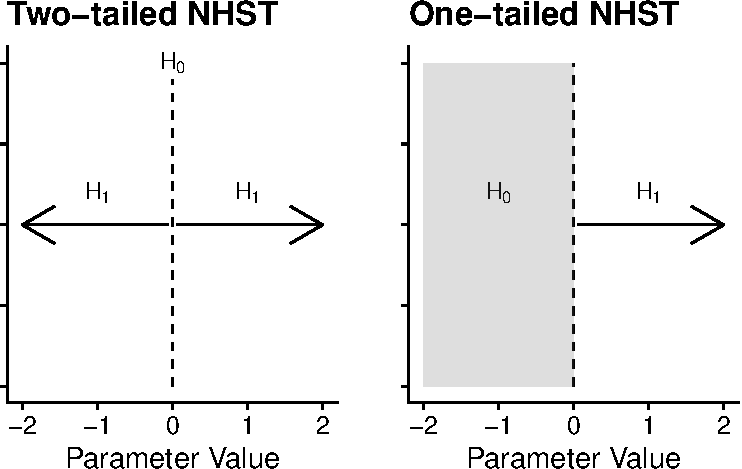
\includegraphics[width=1\textwidth,height=\textheight]{appendix-c-equivalence_files/figure-pdf/unnamed-chunk-2-1.pdf}
\end{center}

In a two-tailed test, the null is precisely zero and you are trying to
reject it in favour of the alternative hypothesis which can be any
positive or negative value. In a one-tailed test, it follows the same
logic, but instead of precisely zero, the null is the entire positive or
negative region, meaning you want to reject values above or below zero
depending which direction you predict. For many research questions, this
logic holds to test for the presence of an effect by rejecting the null
hypothesis. However, what about if your research question / prediction
is interested in testing the null \emph{itself} or a lack of effect?
Unfortunately, you cannot test for the effect being precisely zero but
you can use the procedure to test for effects too small to be
practically or theoretically meaningful.

Equivalence testing (Harms \& Lakens, 2018; Lakens et al., 2018, 2020)
flips the null hypothesis significance testing logic. In this setup, you
set two boundaries representing your smallest effect size of interest
(SESOI) and conduct two one-sided tests: one comparing your test
statistic/value to the upper bound and one comparing your test
statistic/value to the lower bound. If both tests are statistically
significant, you can conclude the mean was within your bounds and it is
practically equivalent to zero.

This procedure is usually referred to by the single name of equivalence
testing, but you can apply it in two ways depending on your research
question. In an equivalence test, you want to test whether your test
statistic/value is smaller than your boundaries, i.e., you want to test
for the absence of an effect. Conversely, in a minimal effects test you
want to test whether your statistic/value is larger than your
boundaries, i.e., you want to test for an effect exceeding your SESOI.

\begin{center}
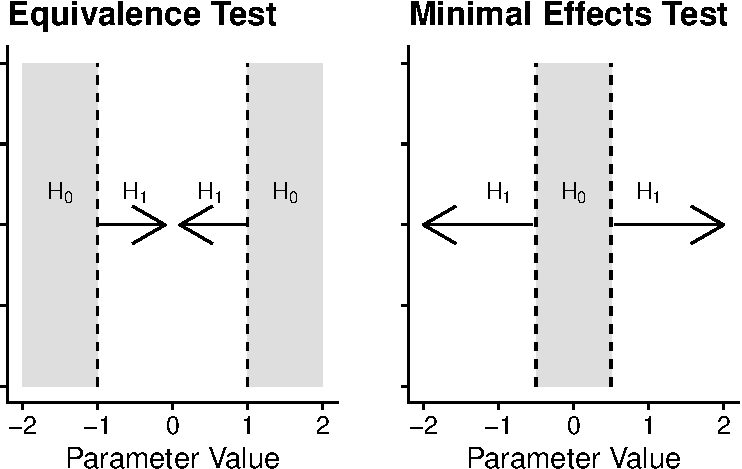
\includegraphics[width=1\textwidth,height=\textheight]{appendix-c-equivalence_files/figure-pdf/unnamed-chunk-3-1.pdf}
\end{center}

In an equivalence test, the null hypothesis is split into two regions
representing your SESOI. The two one-sided tests compare your test
statistic/value to calculate whether it is significantly lower than the
upper bound \textbf{and} significantly higher than the upper bound. If
both tests are significant, you conclude it is statistically equivalent,
given the boundaries you set. Conversely, a minimal effects test flips
this procedure. Instead of a point-null in NHST, the null hypothesis is
a region of effects representing your SESOI. The two one-sided tests
calculate whether your test statistic/value is significantly lower than
the lower bound and significantly higher than the higher bound. You are
looking for the tests to be statistically significant to test the null
region.

Justifying your equivalence/minimal effects bounds is probably the most
difficult decision you will make as it requires subject knowledge for
what you would consider the smallest effect size of interest. For a
non-exhaustive list, there are different strategies like:

\begin{enumerate}
\def\labelenumi{\arabic{enumi}.}
\item
  Your understanding of the applications / mechanisms (e.g., a
  clinically meaningful decrease in pain).
\item
  Smallest effects from previous research (e.g., lower bound of
  individual study effect sizes or lower bound of a meta-analysis).
\item
  Small telescopes (the effect size the original study had 33\% power to
  detect).
\end{enumerate}

\section{Correlations}\label{correlations}

To apply the procedure to correlations, we will use the Dawtry et al.
(2015) data and the relationship between support for wealth
redistribution and perceived fairness and satisfaction in the current
system. For a starting point, we need to calculate the correlation
coefficient as standard.

\begin{Shaded}
\begin{Highlighting}[]
\FunctionTok{correlation}\NormalTok{(}\AttributeTok{data =}\NormalTok{ dawtry\_clean, }
            \AttributeTok{select =} \StringTok{"fairness\_satisfaction"}\NormalTok{, }
            \AttributeTok{select2 =} \StringTok{"redistribution"}\NormalTok{,  }
            \AttributeTok{method =} \StringTok{"pearson"}\NormalTok{, }
            \AttributeTok{alternative =} \StringTok{"two.sided"}\NormalTok{)}
\end{Highlighting}
\end{Shaded}

\begin{verbatim}
# Correlation Matrix (pearson-method)

Parameter1            |     Parameter2 |     r |         95% CI | t(303) |         p
------------------------------------------------------------------------------------
fairness_satisfaction | redistribution | -0.70 | [-0.75, -0.64] | -17.08 | < .001***

p-value adjustment method: Holm (1979)
Observations: 305
\end{verbatim}

\subsection{Equivalence testing}\label{equivalence-testing}

For the first demonstration, we will conduct an equivalence test using
the correlation coefficient we observed. The idea behind this function
is that you can apply the procedure when you only have summary
statistics and you do not need the raw data. In the
\texttt{corsum\_test()} function, we need to define:

\begin{itemize}
\item
  \texttt{r} - The observed correlation coefficient.
\item
  \texttt{n} - The number of observation pairs, i.e., the sample size.
\item
  \texttt{alternative} - The hypothesis to test, including options like
  ``equivalence'' and ``minimal.effect''.
\item
  \texttt{method} - The type of correlation to calculate, including
  options like ``pearson'' and ``spearman''.
\item
  \texttt{null} - The null hypothesis or region to test against. If you
  provide a single value, it will test against symmetrical values, i.e.,
  0.2 will test against -0.2 and 0.2. If you want to specify
  asymmetrical values, you must enter a vector of numbers like
  \texttt{c(0,\ 0.2)}.
\end{itemize}

To apply this procedure to the correlation example, we can enter -0.70
for the Pearson correlation coefficient and 305 participants. The
equivalence bounds is the hardest argument to set here, so we will use
0.2 as there is an idea called the ``crud factor'' where correlations
smaller than 0.2 are likely noise (although Orben \& Lakens (2020)
critique this somewhat).

\begin{Shaded}
\begin{Highlighting}[]
\FunctionTok{corsum\_test}\NormalTok{(}\AttributeTok{r =} \SpecialCharTok{{-}}\FloatTok{0.70}\NormalTok{, }
            \AttributeTok{n =} \DecValTok{305}\NormalTok{, }
            \AttributeTok{alternative =} \StringTok{"equivalence"}\NormalTok{, }
            \AttributeTok{method =} \StringTok{"pearson"}\NormalTok{, }
            \AttributeTok{null =} \FloatTok{0.2}\NormalTok{)}
\end{Highlighting}
\end{Shaded}

\begin{verbatim}

    Pearson's product-moment correlation

data:  x and y
z = -11.549, N = 305, p-value = 1
alternative hypothesis: equivalence
null values:
correlation correlation 
        0.2        -0.2 
90 percent confidence interval:
 -0.7451459 -0.6484676
sample estimates:
 cor 
-0.7 
\end{verbatim}

In this example, the \emph{p}-value of the equivalence test is 1 which
might sound strange, but we need to think of the procedure here.
Remember in an equivalence test we want to test whether the test
statistic is \emph{smaller} than the boundaries. In this scenario, the
observed test statistic is \emph{r} = -0.70 (90\% CI = {[}-0.75,
-0.65{]}). The correlation is pretty large and beyond the lower bound of
-0.2, so it is entirely within that null region.

\begin{tcolorbox}[enhanced jigsaw, breakable, colframe=quarto-callout-note-color-frame, arc=.35mm, opacitybacktitle=0.6, titlerule=0mm, colbacktitle=quarto-callout-note-color!10!white, colback=white, toprule=.15mm, bottomtitle=1mm, toptitle=1mm, title=\textcolor{quarto-callout-note-color}{\faInfo}\hspace{0.5em}{Why is it a 90\% CI?}, bottomrule=.15mm, rightrule=.15mm, leftrule=.75mm, coltitle=black, left=2mm, opacityback=0]

One detail you might have noticed is that we use a 90\% confidence
interval instead of the standard 95\%. If we want to maintain the
standard alpha rate at 5\%, a 90\% confidence interval over two tests
maintains the alpha rate at 5\%.

\end{tcolorbox}

\subsection{Minimal effects testing}\label{minimal-effects-testing}

For this scenario, it would be more aligned with a minimal effects test
as we want to calculate whether our effect exceeds our SESOI. This time,
we will set the alternative argument as \texttt{"minimal.effect"}.

\begin{Shaded}
\begin{Highlighting}[]
\FunctionTok{corsum\_test}\NormalTok{(}\AttributeTok{r =} \SpecialCharTok{{-}}\FloatTok{0.70}\NormalTok{, }
            \AttributeTok{n =} \DecValTok{305}\NormalTok{, }
            \AttributeTok{alternative =} \StringTok{"minimal.effect"}\NormalTok{, }
            \AttributeTok{method =} \StringTok{"pearson"}\NormalTok{, }
            \AttributeTok{null =} \FloatTok{0.2}\NormalTok{)}
\end{Highlighting}
\end{Shaded}

\begin{verbatim}

    Pearson's product-moment correlation

data:  x and y
z = -11.549, N = 305, p-value < 2.2e-16
alternative hypothesis: minimal.effect
null values:
correlation correlation 
        0.2        -0.2 
90 percent confidence interval:
 -0.7451459 -0.6484676
sample estimates:
 cor 
-0.7 
\end{verbatim}

This time, it is statistically significant as our observed correlation
coefficient is significantly lower than our lower bound of -0.2. This
means we can conclude the effect size exceeds our minimal effects test.

\subsection{Plotting the tests}\label{plotting-the-tests}

To help communicate your findings, or just help contextualise things for
you, we can plot the results of these tests using one of two methods.
First, the TOSTER package comes with a function to plot different tests
that we can edit using ggplot2 layers.

The first step is saving the plot object using the same values as we
used for the equivalence test.

\begin{Shaded}
\begin{Highlighting}[]
\NormalTok{p }\OtherTok{\textless{}{-}} \FunctionTok{plot\_cor}\NormalTok{(}\AttributeTok{r =} \SpecialCharTok{{-}}\FloatTok{0.70}\NormalTok{, }
         \AttributeTok{n =} \DecValTok{305}\NormalTok{, }
         \AttributeTok{method =} \StringTok{"pearson"}\NormalTok{, }
         \AttributeTok{type =} \StringTok{"cd"}\NormalTok{)}

\CommentTok{\# print the object}
\NormalTok{p}
\end{Highlighting}
\end{Shaded}

\begin{center}
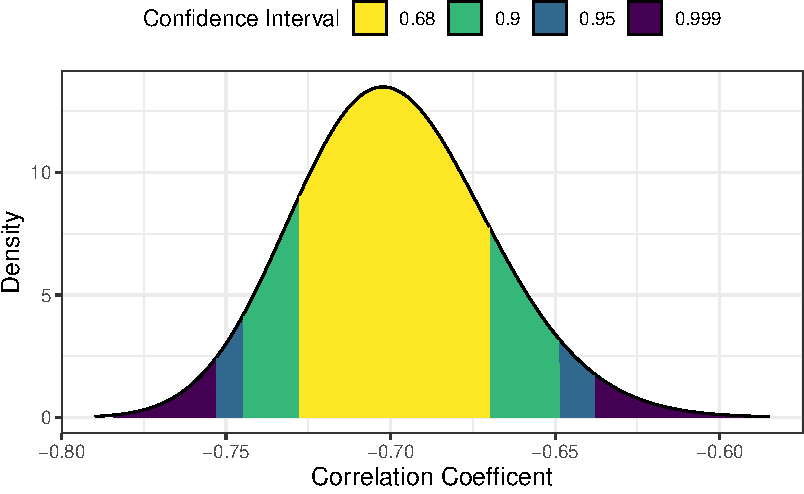
\includegraphics[width=1\textwidth,height=\textheight]{appendix-c-equivalence_files/figure-pdf/unnamed-chunk-7-1.pdf}
\end{center}

The default arguments here visualise the observed correlation
coefficient with a range of confidence intervals. We can then add
ggplot2 layers to visualise the equivalence test or minimal effects test
results, depending which way around you want to interpret the results.

\begin{Shaded}
\begin{Highlighting}[]
\NormalTok{p }\SpecialCharTok{+} \FunctionTok{scale\_x\_continuous}\NormalTok{(}\AttributeTok{limits =} \FunctionTok{c}\NormalTok{(}\SpecialCharTok{{-}}\FloatTok{0.8}\NormalTok{, }\FloatTok{0.2}\NormalTok{), }
                       \AttributeTok{breaks =} \FunctionTok{seq}\NormalTok{(}\SpecialCharTok{{-}}\FloatTok{0.8}\NormalTok{, }\FloatTok{0.2}\NormalTok{, }\FloatTok{0.2}\NormalTok{)) }\SpecialCharTok{+} 
  \FunctionTok{annotate}\NormalTok{(}\AttributeTok{geom =} \StringTok{"rect"}\NormalTok{, }
           \AttributeTok{xmin =} \SpecialCharTok{{-}}\FloatTok{0.2}\NormalTok{, }\AttributeTok{xmax =} \FloatTok{0.2}\NormalTok{, }
           \AttributeTok{ymin =} \FunctionTok{I}\NormalTok{(}\DecValTok{0}\NormalTok{), }\AttributeTok{ymax =} \FunctionTok{I}\NormalTok{(}\DecValTok{100}\NormalTok{), }\CommentTok{\# I() specifies values as percent of plot}
           \AttributeTok{alpha =} \FloatTok{0.4}\NormalTok{)}
\end{Highlighting}
\end{Shaded}

\begin{center}
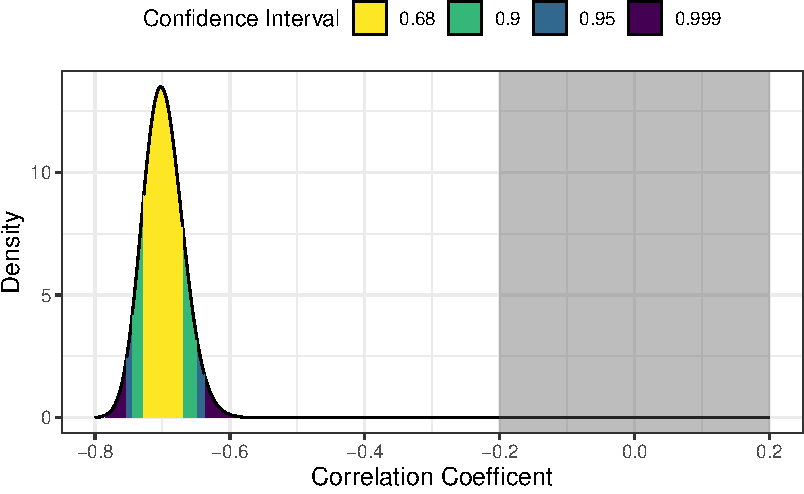
\includegraphics[width=1\textwidth,height=\textheight]{appendix-c-equivalence_files/figure-pdf/unnamed-chunk-8-1.pdf}
\end{center}

Alternatively, if you wanted a more minimalist look or you wanted to
plot the results of multiple correlations, we can create our own
version. The first step is saving the results of a
\texttt{correlation()} object, specifying we want the 90\% confidence
interval.

\begin{Shaded}
\begin{Highlighting}[]
\NormalTok{save\_correlation }\OtherTok{\textless{}{-}} \FunctionTok{correlation}\NormalTok{(}\AttributeTok{data =}\NormalTok{ dawtry\_clean, }
            \AttributeTok{select =} \StringTok{"fairness\_satisfaction"}\NormalTok{, }
            \AttributeTok{select2 =} \StringTok{"redistribution"}\NormalTok{,  }
            \AttributeTok{method =} \StringTok{"pearson"}\NormalTok{, }
            \AttributeTok{alternative =} \StringTok{"two.sided"}\NormalTok{,}
            \AttributeTok{ci =} \FloatTok{0.9}\NormalTok{)}
\end{Highlighting}
\end{Shaded}

This provides us with a data frame containing one row. This means we can
take the results and feed it into ggplot2. We can use similar layers to
customise our own version of the plot to help visualise the equivalence
or minimal effects test.

\begin{Shaded}
\begin{Highlighting}[]
\NormalTok{save\_correlation }\SpecialCharTok{\%\textgreater{}\%} 
  \FunctionTok{ggplot}\NormalTok{(}\FunctionTok{aes}\NormalTok{(}\AttributeTok{y =}\NormalTok{ r, }\AttributeTok{x =} \StringTok{""}\NormalTok{)) }\SpecialCharTok{+} \CommentTok{\# leave x blank}
  \FunctionTok{geom\_point}\NormalTok{() }\SpecialCharTok{+} \CommentTok{\# correlation estimate}
  \FunctionTok{geom\_errorbar}\NormalTok{(}\FunctionTok{aes}\NormalTok{(}\AttributeTok{ymin =}\NormalTok{ CI\_low, }\CommentTok{\# 90\% CI around r}
                    \AttributeTok{ymax =}\NormalTok{ CI\_high), }
                \AttributeTok{width =} \FloatTok{0.2}\NormalTok{) }\SpecialCharTok{+} 
  \FunctionTok{labs}\NormalTok{(}\AttributeTok{x =} \StringTok{""}\NormalTok{,}
       \AttributeTok{y =} \StringTok{"Pearson\textquotesingle{}s Correlation"}\NormalTok{) }\SpecialCharTok{+} 
  \FunctionTok{coord\_flip}\NormalTok{() }\SpecialCharTok{+} \CommentTok{\# flip x and y axes}
  \FunctionTok{scale\_y\_continuous}\NormalTok{(}\AttributeTok{limits =} \FunctionTok{c}\NormalTok{(}\SpecialCharTok{{-}}\FloatTok{0.8}\NormalTok{, }\FloatTok{0.2}\NormalTok{), }
                       \AttributeTok{breaks =} \FunctionTok{seq}\NormalTok{(}\SpecialCharTok{{-}}\FloatTok{0.8}\NormalTok{, }\FloatTok{0.2}\NormalTok{, }\FloatTok{0.2}\NormalTok{)) }\SpecialCharTok{+} 
  \FunctionTok{annotate}\NormalTok{(}\AttributeTok{geom =} \StringTok{"rect"}\NormalTok{, }\CommentTok{\# add the box for the SESOI}
           \AttributeTok{ymin =} \SpecialCharTok{{-}}\FloatTok{0.2}\NormalTok{, }\AttributeTok{ymax =} \FloatTok{0.2}\NormalTok{, }
           \AttributeTok{xmin =} \FunctionTok{I}\NormalTok{(}\DecValTok{0}\NormalTok{), }\AttributeTok{xmax =} \FunctionTok{I}\NormalTok{(}\DecValTok{100}\NormalTok{),}
           \AttributeTok{alpha =} \FloatTok{0.4}\NormalTok{)}
\end{Highlighting}
\end{Shaded}

\begin{center}
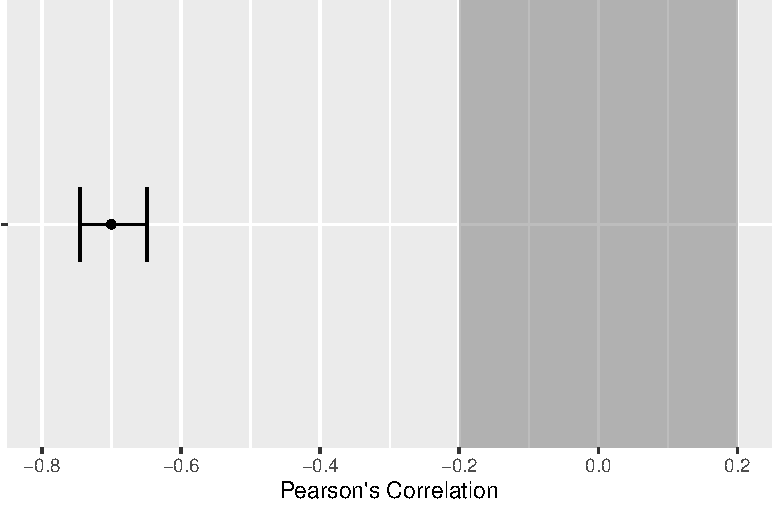
\includegraphics[width=1\textwidth,height=\textheight]{appendix-c-equivalence_files/figure-pdf/unnamed-chunk-10-1.pdf}
\end{center}

\section{t-tests}\label{t-tests}

To apply the procedure to t-tests, we will use the Lopez et al. (2023)
data and the difference in calories consumed between accurate and
inaccurate visual cues.

\subsection{Equivalence testing}\label{equivalence-testing-1}

There are two ways you can apply the equivalence testing procedure for
t-tests. We are focusing on two groups here, but the function also works
for paired samples and one-sample t-tests. We will start with the
\texttt{t\_TOST()} function which starts with similar arguments to the
standard \texttt{t.test()} function:

\begin{itemize}
\item
  \texttt{formula} - For two groups, we can use the standard
  \texttt{outcome\ \textasciitilde{}\ predictor} format. If you have
  paired samples or one-sample, you can use the \texttt{x} and
  \texttt{y} arguments.
\item
  \texttt{data} - The data frame you are using.
\item
  \texttt{eqb} - The equivalence bounds you want to set. If you enter
  one number, it will create symmetrical bounds, such as -20 to 20. If
  you want asymmetrical bound, you would need to enter a vector of
  numbers.\\
\item
  \texttt{eqbound\_type} - The default option is to enter ``raw'' units,
  so whatever scale your outcome is on. For our example, this will be in
  calories. Your other option is ``smd'' for standardised mean
  difference, or Cohen's d.~You can enter the equivalence bounds as
  standardised units but it comes with a little warning that there is
  potential bias.\\
\item
  \texttt{hypothesis} - This is where you can create an equivalence test
  using ``EQU'' or a minimal effects test using ``MET''. We will come
  back to minimal effects in the next section.
\end{itemize}

The main argument to explain here is using 57 calories for the
equivalence bounds. Remember this is a t-test, so we want to see whether
one group is larger (or smaller) than the other. Setting the equivalence
bounds is the single most difficult part here but Lopez et al. (2023)
explain that they were interested in detecting an effect at least half
as large as the original Wansink et al.~study. Therefore, in an
equivalence test, we would ask the question whether the observed effect
size is smaller than 57 calories difference.

\begin{Shaded}
\begin{Highlighting}[]
\FunctionTok{t\_TOST}\NormalTok{(}\AttributeTok{formula =}\NormalTok{ F\_CaloriesConsumed }\SpecialCharTok{\textasciitilde{}}\NormalTok{ Condition\_label, }
       \AttributeTok{data =}\NormalTok{ lopez\_clean, }
       \AttributeTok{eqb =} \DecValTok{57}\NormalTok{, }
       \AttributeTok{eqbound\_type =} \StringTok{"raw"}\NormalTok{,}
       \AttributeTok{hypothesis =} \StringTok{"EQU"}\NormalTok{)}
\end{Highlighting}
\end{Shaded}

\begin{verbatim}

Welch Two Sample t-test

The equivalence test was non-significant, t(453.45) = -0.47, p = 0.68
The null hypothesis test was significant, t(453.45) = -4.86, p < 0.01
NHST: reject null significance hypothesis that the effect is equal to zero 
TOST: don't reject null equivalence hypothesis

TOST Results 
                 t    df p.value
t-test     -4.8578 453.4 < 0.001
TOST Lower -0.4661 453.4   0.679
TOST Upper -9.2495 453.4 < 0.001

Effect Sizes 
               Estimate       SE                 C.I. Conf. Level
Raw            -63.0495 12.97908 [-84.4419, -41.6571]         0.9
Hedges's g(av)  -0.4513  0.09445   [-0.6059, -0.2963]         0.9
Note: SMD confidence intervals are an approximation. See vignette("SMD_calcs").
\end{verbatim}

The output is busier than correlations, so we will walk through the
three sections. The first explains the summary of the equivalence tests.
You get both the equivalence test and a traditional t-test. Here, the
traditional t-test is significant (we can reject 0) but the equivalence
test is non-significant, meaning we cannot conclude the effect was
statistically equivalent, given our bounds.

The second section adds context to this as you see the output for all
three tests. The t-test is significant to reject zero. We then have the
two one-sided tests where one is significant (we can reject the upper
bound), but the other is non-significant. Both need to be significant to
conclude equivalence.

Finally, we have a summary of the effect sizes. You get the raw /
unstandardised effect size and it's 90\% CI. For our equivalence bounds
of -57 to 57, the upper bound of the 90\% CI (-41.66) extends into the
equivalence bounds, so that's why the test is non-significant. You also
get Hedge's g as a standardised effect size.

Briefly, there is a second, more minimalist function to calculate the
equivalence test called \texttt{simple\_htest()}. This is supposed to
look closer to the output from a traditional t-test but the conclusion
is the same. You just get one test (the smaller of the two one-sided
tests) and a summary of the boundaries.

\begin{Shaded}
\begin{Highlighting}[]
\FunctionTok{simple\_htest}\NormalTok{(}\AttributeTok{formula =}\NormalTok{ F\_CaloriesConsumed }\SpecialCharTok{\textasciitilde{}}\NormalTok{ Condition\_label, }
       \AttributeTok{data =}\NormalTok{ lopez\_clean, }
       \AttributeTok{mu =} \DecValTok{57}\NormalTok{, }
       \AttributeTok{alternative =} \StringTok{"e"}\NormalTok{)}
\end{Highlighting}
\end{Shaded}

\begin{verbatim}

    Welch Two Sample t-test

data:  F_CaloriesConsumed by Condition_label
t = -0.4661, df = 453.45, p-value = 0.6793
alternative hypothesis: equivalence
null values:
difference in means difference in means 
                -57                  57 
90 percent confidence interval:
 -84.44188 -41.65710
sample estimates:
mean of x mean of y 
 196.6818  259.7313 
\end{verbatim}

\subsection{Minimal effects testing}\label{minimal-effects-testing-1}

For the framing of Lopez et al. (2023), it potentially makes more sense
to calculate a minimal effects test if we are interested in the effect
being at least as large as half the original effect size. In other
words, we want to see whether the effect is 57 calories or greater,
rather than smaller than 57 calories.

\begin{Shaded}
\begin{Highlighting}[]
\FunctionTok{t\_TOST}\NormalTok{(}\AttributeTok{formula =}\NormalTok{ F\_CaloriesConsumed }\SpecialCharTok{\textasciitilde{}}\NormalTok{ Condition\_label, }
       \AttributeTok{data =}\NormalTok{ lopez\_clean, }
       \AttributeTok{eqb =} \DecValTok{57}\NormalTok{, }
       \AttributeTok{eqbound\_type =} \StringTok{"raw"}\NormalTok{,}
       \AttributeTok{hypothesis =} \StringTok{"MET"}\NormalTok{)}
\end{Highlighting}
\end{Shaded}

\begin{verbatim}

Welch Two Sample t-test

The minimal effect test was non-significant, t(453.45) = -9.2, p = 0.32
The null hypothesis test was significant, t(453.45) = -4.86, p < 0.01
NHST: reject null significance hypothesis that the effect is equal to zero 
TOST: don't reject null MET hypothesis

TOST Results 
                 t    df p.value
t-test     -4.8578 453.4 < 0.001
TOST Lower -0.4661 453.4   0.321
TOST Upper -9.2495 453.4       1

Effect Sizes 
               Estimate       SE                 C.I. Conf. Level
Raw            -63.0495 12.97908 [-84.4419, -41.6571]         0.9
Hedges's g(av)  -0.4513  0.09445   [-0.6059, -0.2963]         0.9
Note: SMD confidence intervals are an approximation. See vignette("SMD_calcs").
\end{verbatim}

In changing the \texttt{hypothesis} argument to ``MET'', we still get
all the same output but the framing changes. Instead of testing whether
the observed effect is \emph{within} the equivalence bounds, we test
whether the effect is \emph{outwith} the equivalence bounds. We get a
similar conclusion here where the traditional t-test is significant and
we can reject the point null of zero. However, the minimal effects test
is non-significant and our effect does not exceed the bounds.

\subsection{Plotting the tests}\label{plotting-the-tests-1}

The plotting options are also a little nicer here as there are built-in
visualisations for equivalence tests. First, we need to save the initial
test object.

\begin{Shaded}
\begin{Highlighting}[]
\NormalTok{lopez\_EQU }\OtherTok{\textless{}{-}} \FunctionTok{t\_TOST}\NormalTok{(}\AttributeTok{formula =}\NormalTok{ F\_CaloriesConsumed }\SpecialCharTok{\textasciitilde{}}\NormalTok{ Condition\_label, }
                    \AttributeTok{data =}\NormalTok{ lopez\_clean, }
                    \AttributeTok{eqb =} \DecValTok{57}\NormalTok{, }
                    \AttributeTok{eqbound\_type =} \StringTok{"raw"}\NormalTok{,}
                    \AttributeTok{hypothesis =} \StringTok{"EQU"}\NormalTok{)}
\end{Highlighting}
\end{Shaded}

We can then pass the object to \texttt{plot()} to create different types
of visualisation. The first is a simple dot-and-whisker plot we created
ourselves for the correlation.

\begin{Shaded}
\begin{Highlighting}[]
\FunctionTok{plot}\NormalTok{(lopez\_EQU, }
     \AttributeTok{type =} \StringTok{"simple"}\NormalTok{, }
     \AttributeTok{layout =} \StringTok{"combined"}\NormalTok{)}
\end{Highlighting}
\end{Shaded}

\begin{center}
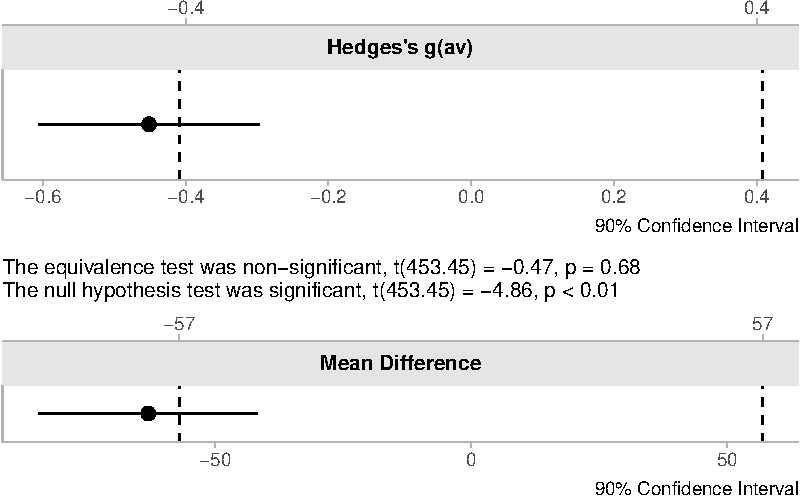
\includegraphics[width=1\textwidth,height=\textheight]{appendix-c-equivalence_files/figure-pdf/unnamed-chunk-15-1.pdf}
\end{center}

The second is a density plot like we saw for correlations, but this time
the equivalence bounds are added automatically.

\begin{Shaded}
\begin{Highlighting}[]
\FunctionTok{plot}\NormalTok{(lopez\_EQU, }
     \AttributeTok{type =} \StringTok{"cd"}\NormalTok{)}
\end{Highlighting}
\end{Shaded}

\begin{center}
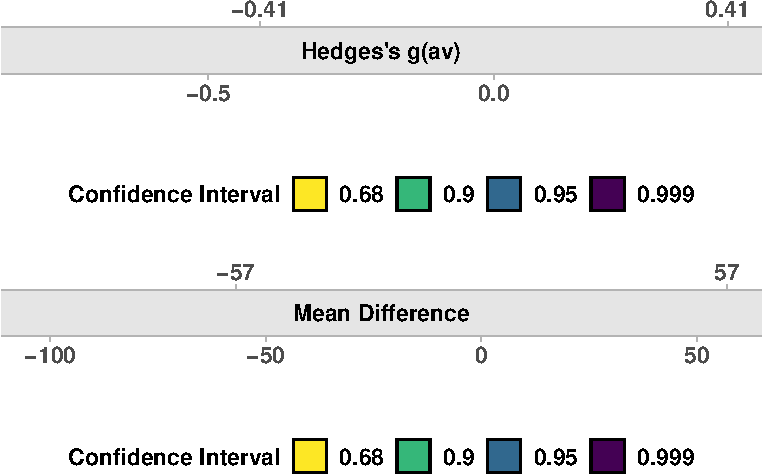
\includegraphics[width=1\textwidth,height=\textheight]{appendix-c-equivalence_files/figure-pdf/unnamed-chunk-16-1.pdf}
\end{center}

Both visualisations reinforce the conclusion that we have a
traditionally significant result where we can reject a point-null, but
the effect estimate and it's precision through the 90\% CI does not
exceed the equivalence bounds we set.




\end{document}
